\documentclass[openany,twocolumn]{amsbook}
\usepackage[utf8]{inputenc}
\setcounter{tocdepth}{2}
\title{A Survey of Partially Ordered Algebras}
\author{Peter Jipsen and Bianca Newell}
\author{\url{jipsen@chapman.edu}, \url{bnewell@chapman.edu}}
\author{DRAFT version: \url{math.chapman.edu/~jipsen/Survey-of-po-algebras-DRAFT.pdf}}
\address{\hspace{1.3in}Version 0.3, 2021 November 14, Chapman University}

\usepackage{natbib}
\usepackage[margin=1in]{geometry}
\usepackage[colorlinks=true,linkcolor=blue,citecolor=brown]{hyperref}
\usepackage{tikz}
\usepackage{amsthm}
\usepackage{amsmath}
\usepackage{amssymb}
%\usepackage{longtable}
%\usepackage{multicol}
%\usepackage{supertabular}

\newenvironment{definition}{\textbf{Definition}\par}{\par}
\newenvironment{fulldefinition}{\textbf{Formal Definition}\par}{\par}
\newenvironment{basicresults}{\textbf{Basic Results}\par}{\par}
\newenvironment{examples}{\textbf{Examples}\par}{\par}
\newenvironment{properties}{\textbf{Properties}\par}{\par}
\newenvironment{finitemembers}{\textbf{Finite Members}\par}{\par}
\newenvironment{smallmembers}{\textbf{Small Members} (not in any subclass)\par}{\par}
\newenvironment{subclasses}{\textbf{Subclasses}\par}{\par}
\newenvironment{superclasses}{\textbf{Superclasses}\par}{\hfill
\hyperlink{tocontents}{Cont}$|$\hyperlink{Po}{Po}$|$\hyperlink{J}{J}$|$\hyperlink{M}{M}$|$\hyperlink{L}{L}$|$\hyperlink{D}{D}$|$\hyperlink{To}{To}$|$\hyperlink{B}{B}$|$\hyperlink{U}{U}$|$\hyperlink{toindex}{Ind}\par}

\newtheorem{theorem}{Theorem}
\newtheorem{lemma}[theorem]{Lemma}
\newcommand{\cl}{\mathcal}
\newcommand{\m}{\mathbf}
\newcommand{\s}{\mathsf}
\newcommand{\co}{\smallsmile}
\newcommand{\ua}{{\uparrow}}
\newcommand{\da}{{\downarrow}}
\newcommand{\cemph}[1]{\textcolor{red}{{\em #1\/}}}
%\renewcommand{\langle}{(}
%\renewcommand{\rangle}{)}
\newcommand{\alg}[1]{(#1)}
\newcommand{\abbreviation}[1]{Abbreviation: \textbf{#1}}
\newcommand{\dotdiv}{\mathbin{\overset{\raisebox{.5ex}{.}}{\smash{-}}}}
\renewcommand{\emph}[1]{{\it #1\index{#1}\/}}
\newcommand{\g}{\textcolor{blue}}
\newcommand{\rd}[1]{\textcolor{red}{\boldsymbol{#1}}}
\newcommand{\rn}{\rule[2pt]{3pt}{.5pt}\mkern1mu}
\newcommand{\W}[1]{\makebox[12pt]{$#1$}}%
\arraycolsep0pt

\includeonly{
SoPoAchapters,
SoPoAappendix
}
\makeindex


\begin{document}
\tikzstyle{every node} = [draw, fill=white, circle, inner sep=0pt, minimum size=5pt]
\tikzstyle{d} = [very thick]
\tikzstyle{n} = [draw=none, rectangle, inner sep=2pt] %name style
\tikzstyle{i} = [draw, fill=black, circle, inner sep=0pt, minimum size=5pt] %idempotent
\onecolumn
\maketitle

\hypertarget{tocontents}{}
\tableofcontents

\chapter{Introduction}
\noindent
\subsection*{Disclaimer: This project is currently in a DRAFT stage. For some classes of algebras it may contain incomplete and/or incorrect information. In particular, the introduction needs to be (re)written.}

\ 

This survey of partially ordered algebras contains
definitions and descriptions of many algebraic categories. 
The most general classes of algebraic structures covered here 
are partially ordered sets with finitary operations that
preserve or reverse the partial order in each argument. These
structures are known as \emph{po-algebras}, and they form a category with morphisms that are order-preserving homomorphisms. While
po-algebras are not purely algebraic, their (in)equational theory is a relatively straight forward extension of universal algebra.
The details can be found in \cite{Pig2004}, but we (will eventually) also cover the main points below. 

Chapter 2 contains the main classes of po-algebras. Every class has a definition with quasi-inequalities that indicate for each argument of each fundamental operation whether it is 
\begin{align*}
\text{order-preserving: \ } &x\le y\implies f(z_1,\ldots,z_{i-1},x,z_{i+1},\ldots,z_n)\le f(z_1,\ldots,z_{i-1},y,z_{i+1}\ldots,z_n)\text{ or}\\
\text{order-reversing: \ } &x\le y\implies f(z_1,\ldots,z_{i-1},x,z_{i+1},\ldots,z_n)\ge f(z_1,\ldots,z_{i-1},y,z_{i+1}\ldots,z_n).
\end{align*}
If the operation has
(left/right) residuals this behaviour can also be inferred from
the residuation property.
In Chapter 3 we cover classes of join-semilattice ordered algebras, followed by classes of meet-semilattice ordered algebras in Chapter 4. Since joins and meets can both be used to
define the partial order by an equation, these classes are purely algebraic and are entirely within the realm of universal algebra.
However, we now also record if an argument of a fundamental operation is join/meet-preserving, and we continue to use the perspective of po-algebras since it captures the close connections between proof theory and inequational logic.
Chapter 5 contains lattice-ordered algebras, with fundamental operations that preserve join and/or meets, or reverse joins and/or meets in each argument. To say that an $n$-ary operation $f$ \emph{reverses joins} in the $i$th argument means that
$$
f(z_1,\ldots,z_{i-1},x\vee y,z_{i+1},\ldots,z_n)=f(z_1,\ldots,z_{i-1},x,z_{i+1}\ldots,z_n)\wedge f(z_1,\ldots,z_{i-1},y,z_{i+1},\ldots,z_n)
$$
and dually for \emph{reversing meets}. Any operation that preserves all joins or all meets in an argument is automatically order-preserving in that argument, and likewise any operation that reverses all joins or all meets in an argument is automatically order-reversing in that argument.

The following diagram shows the highest level of our classification of categories of partially ordered algebras, numbered by the corresponding chapter number. 


\begin{center}
\begin{tikzpicture}[xscale=6]
%\node(in)at(0,6)[n]{1. Introduction};
\node(po)at(0,5)[n]{2. Partially ordered algebras};
\node(jsl)at(-1,4)[n]{3. Join-semilattice ordered};
\node(msl)at(0,4)[n]{4. Meet-semilattice ordered};
\node(lat)at(-1,3)[n]{5. Lattice-ordered algebras};
\node(dl)at(-1,2)[n]{6. Distributive lattice-ordered algebras};
\node(to)at(-1,1)[n]{7. Totally ordered algebras};
\node(ba)at(0,1)[n]{8. Boolean ordered algebras};
\node(uo)at(1,2.5)[n]{9. Unordered algebras};
\node(0)at(0,0)[n]{Trivial algebras};
\draw(0)--(ba)--(dl)--(to)--(0)--(uo)--(po)--(jsl)--(lat)--(msl)--(po);
\draw(lat)--(dl);
\end{tikzpicture}
\end{center}


\begin{figure}
\begin{center}
\tikzstyle{p} = [draw=red, fill=white, circle, inner sep=4pt, minimum size=5pt]
\begin{tikzpicture}[xscale=4,yscale=2]
\node(po)at(0,5)[p,label=left:Po$\ $]{\begin{tikzpicture}[scale=.5]\draw(0,0)node{}--(0,1)node{};\draw(1,.5)node{};\end{tikzpicture}};
\node(jsl)at(-1,4)[p,label=left:J$\ $]{\begin{tikzpicture}[scale=.5]\draw(-.5,0)node{}--(0,1)node{}--(.5,0)node{};\end{tikzpicture}};
\node(msl)at(0,4)[p,label=left:M$\ $]{\begin{tikzpicture}[scale=.5]\draw(-.5,1)node{}--(0,0)node{}--(.5,1)node{};\end{tikzpicture}};
\node(lat)at(-1,3)[p,label=left:$\ell\ $]{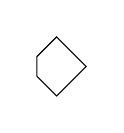
\begin{tikzpicture}[scale=.5]\draw(-.5,.5)--(0,0)node{}--(.75,.75)node{}--(0,1.5)node{}--(-.5,1)node{}--(-.5,.5)node{};\end{tikzpicture}};
\node(dl)at(-1,2)[p,label=left:D$\ $]{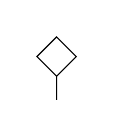
\begin{tikzpicture}[scale=.5]\draw(0,-.1)node{}--(0,.5)--(.5,1)node{}--(0,1.5)node{}--(-.5,1)node{}--(0,.5)node{};\end{tikzpicture}};
\node(to)at(-1,1)[p,label=left:To$\ $]{\begin{tikzpicture}[scale=.5]\draw(0,0)node{}--(0,.75)node{}--(0,1.5)node{};\end{tikzpicture}};
\node(uo)at(1.3,2.5)[p]{\begin{tikzpicture}[scale=.5]\draw(0,0)node{};\draw(.7,0)node{};\draw(1.4,0)node{};\end{tikzpicture}};
\node(0)at(0,0)[p]{\begin{tikzpicture}[scale=.5]\draw(0,0)node{};\end{tikzpicture}};
\tikzstyle{p} = [draw=red, fill=white, circle, inner sep=2pt, minimum size=5pt]
\node(ba)at(0,1)[p,label=left:B$\ $]{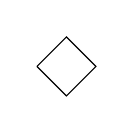
\begin{tikzpicture}[scale=.5]\draw(-.75,.75)--(0,0)node{}--(.75,.75)node{}--(0,1.5)node{}--(-.75,.75)node{};\end{tikzpicture}};
\draw(0)--(ba)--(dl)--(to)--(0)--(uo)--(po)--(jsl)--(lat)--(msl)--(po);
\draw(lat)--(dl);
\end{tikzpicture}
\end{center}
\caption{Examples of a small poset from each chapter}
\end{figure}

Many of the algebras we consider have a binary operation $\cdot$, and the next level of classification is based on whether this operation is commutative. Categories that contain noncommutative algebras precede the commutative ones.

The third level of classification is along an axis of residuation for the operation $\cdot$ in the order: nonresiduated, left-residuated, residuated, involutive, and cyclic involutive.

The fourth level considers whether $\cdot$ is nonassociative, associative, unital, integral, and/or idempotent. Combinations of these properties produce a framework of roughly 50 categories in each of the eight chapters, which are then augmented by several other standard categories that satisfy additional properties. Altogether the survey currently contains (some very basic) information about $\sim$500 categories, with links in the pdf-file that are useful for browsing and comparing closely related categories.

Recall that the fine spectrum of a class of algebras is a sequence of natural numbers $f_n$ such that up to isomorphism there are exactly $f_n$ many algebras of size $n$ in the class.
One of the features of this survey is that for most classes the fine spectrum has been calculated (usually only up to a small value of $n$). In particular for the linearly ordered algebras this sequence is sometimes (related to) a sequence in the Online Encyclopedia of Integer Sequences (\url{OEIS.org}), in which case the entry in the OEIS can lead to additional references and combinatorial results relevant to these algebras.

The github page for this survey also contains some Jupyter notebooks with short Python programs that can extract and check information about the categories. It is likely that the survey will be updated from time-to-time, with the latest version (and a record of the changes) available on github.

The starting point for this survey was an online collection of web pages about classes of mathematical structures that can still be found at \url{math.chapman.edu/~jipsen/mathstructures}. In this pdf-file we concentrate on finitely axiomatized classes of partially ordered algebras and also provide some lists of finite algebras that separate many of these classes.

The signature of po-algebras in this survey mostly uses operations symbols from a fixed set, with arity $\le 2$ and with a specific order type for each argument. The convention is given in Table~\ref{ordtypes}. 

In addition we adopt the following convention: \textbf{If a po-algebra does not have a join operation $\vee$ then any operation  join-preserving order type defaults to order-preserving, and the join-reversing order type defaults to order-reversing.}

E.g., a jsl-semigroup and $\ell$-semigroup have a binary operation $\cdot$ that is join-preserving in both arguments,
but in an msl-semigroup or a po-semigroup the operation $\cdot$
is only order-preserving in each argument.

An operation $\cdot$ on a poset is \emph{residuated} if there exist binary operations $\backslash,/$ such that 
$$
xy\le z\iff y\le x\backslash z\iff x\le z/y.
$$
It is worth noting that such a residuated operation $\cdot$ automatically preserves all existing joins, hence is order-preserving. Its left and right residual $\backslash,/$ preserve all existing meets in the numerator and reverse all existing joins to meets in the denominator.

%Disclaimer: This survey is under revision. The latest version is at \url{www1.chapman.edu/~jipsen/SPoA.pdf} and may be different from the version that you are currently looking at. 

\begin{figure}
\begin{tabular}{|c|c|c|}\hline
Symbols & arity & order type \\\hline
$\cdot, \odot, \circ, ;$ & 2 & join-preserving, join-preserving \\
$+, \oplus$ & 2 & meet-preserving, meet-preserving \\
$\to, \backslash$ & 2 & join-reversing, meet-preserving \\
$/$ & 2 & meet-preserving, join-reversing \\
$\dotdiv$ & 2 & meet-reversing, join-preserving \\
$f, \Diamond, ^\smallsmile$ & 1 & join-preserving \\
$g, \square$ & 1 & meet-preserving \\
$\sim,-$ & 1 & join-reversing \\
$^{-1}$ & 1 & join-and-meet-reversing \\
\hline
\end{tabular}
\centering
\caption{Order types of operation symbols}
\label{ordtypes}
\end{figure}

% Most of these categories are defined by (in)equational axioms and have structure preserving morphisms. In particular, the morphisms are always order-preserving.

% An inequation is an expression of the form $s\le t$ where $s,t$ are terms in some signature. In general, inequations are assumed to be universally quantified over all the variables that appear in them.

\section{Universal algebra and category theory}

\subsection{Algebras and subalgebras} 

An $n$-ary \emph{operation} on a nonempty set $A$ is a function $f:A^n\to A$. Each $n$-ary function on $A$ has a corresponding arity (or rank): nullary operations have arity 0 and are \emph{constants} (fixed elements of $A$), unary operations have arity 1, binary operations have arity 2, and so on. 

An \emph{algebra} $\m A=(A,f^\m A_1,f^\m A_2,\ldots)$ is a set $A$ with operations $f^\m A_i$ of arity $n_i\in\mathbb N$. %Algebras are differentiated by the identities that the operations satisfy. 
The \emph{signature} of an algebra is its list of operation arities $(n_1,n_2,\ldots)$. Operations are usually listed in descending order of their arity.
	
Let $f$ be an operation on a set $A$ and $g$ an operation of the same arity on a subset $B$ of $A$. Then \emph{$g$ is the restriction of $f$ to $B$}, written $g=f|_B$, if for all $b_i\in B$,\quad $g(b_1,\ldots,b_n)=f(b_1,\ldots,b_n)$. 

An algebra $\m B$ is a \emph{subalgebra} of $\m A$ if $B\subseteq A$ and $f^\m B_i=f^\m A_i|_B$ \quad (for all $i$). In other words, $B$ is closed under all operations of $\m A$.

\subsection{Homomorphisms and isomorphisms}

Let $\m A$, $\m B$ be algebras of the same signature. A \emph{homomorphism} $h:\m A\to\m B$ is a function $h:A\to B$ such that for all $i$ $$h(f_i^\m A(a_1,\ldots,a_{n_i})=f_i^\m B(h(a_1),\ldots,h(a_{n_i})).$$

As usual, $h$ is \emph{surjective} or \emph{onto} if $h[A]=\{h(a)\mid a\in A\}=B$. In this case $\m B=h[\m A]$ is called a \emph{homomorphic image} of $\m A$.

A homomorphism $h$ is \emph{one-to-one} if for all $x,y\in A$,\quad $x\ne y$ implies $h(x)\ne h(y)$, and $h$ is an \emph{isomorphism} if $h$ is a one-to-one and onto homomorphism. In this case $\m A$ is said to be \emph{isomorphic} to $\m B$, written $\m A\cong\m B$.

\subsection{Products and HSP}

Products of algebras can combine multiple algebras into one larger algebra. The \emph{cartesian product} of two algebras $\m A_1$ and $\m A_2$ is defined as the set $A_1 \times A_2$ with $a_j \in A_1$ and $a'_j \in A_2$ with an operation $f$ such that $f^{\m A_1 \times \m A_2}$($\langle a_1,a'_1\rangle,...,\langle a_n,a'_n\rangle$) = $\langle f^{\m A_1}(a_1,...,a_n),f^{\m A_2}(a'_1,...,a'_n)\rangle$ for $1\le j\le n$.


The \emph{direct product} of algebras $\m A_j$ ($j \in J$) is $\m A=\prod_{j\in J}\m A_j$ where $A=\prod_{j\in J}A_j$ and $f_i^\m A(a_1,\dots,a_{n_i})(j)= f_i^{\m A_j}(a_1(j),\dots,a_{n_i}(j))$ for all $j \in J$.

Let $\cl K$ be a class of algebras of the same signature. 

\begin{itemize}
    \item $H(\cl K)$ is the class of \textbf{\emph{homomorphic images}} of members of $\cl K$.
    \item $S(\cl K)$ is the class of algebras isomorphic to \textbf{\emph{subalgebras}} of members of $\cl K$.
    \item $P(\cl K)$ is the class of algebras isomorphic to \textbf{\emph{direct products}} of members of $\cl K$.
\end{itemize}  
$\cl K$ is a \emph{variety} if $H(\cl K)=S(\cl K)=P(\cl K)=\cl K$\quad (${\iff} HSP(\cl K)=\cl K$) \cite{Tar1946}.

\subsection{Term algebras and equational classes}
For a fixed signature, the \emph{set of terms with variables from a set $X$} is the smallest set $T(X)$ such that $X\subseteq T(X)$ and $$\text{if $t_1,\dots,t_{n_i}\in T(X)$ then ``$f_i(t_1,\dots,t_{n_i})$'' $\in T(X)$ for all $i$}.$$

The \emph{term algebra over a set $X$} is 
$\m T(X)=(T(X),f_1^\m T,f_2^\m T,\ldots)$ with $$f_i^\m T(t_1,\dots,t_{n_i})=\text{``}f_i(t_1,\dots,t_{n_i})\text{''\quad for all $i$ and $t_1,\dots,t_{n_i}\in T(X)$}.$$

An \emph{equation} is a pair of terms $(s,t)$, written $s{=}t$. An \emph{assignment} into an algebra $\m A$ is a homomorphism $h:\m T(X)\to\m A$. An algebra $\m A$ \emph{satisfies} $s{=}t$ if $h(s)=h(t)$ for all assignments into $\m A$. For a set $E$ of equations, Mod$(E)=\{\m A\mid \m A\text{ satisfies }s{=}t$ for all $s{=}t\in E\}$. An \emph{equational class} is of the form Mod$(E)$ for some set of equations $E$.

\subsection{Varieties and equational logic}
$HSP$ ``preserves'' equations, so every equational class is a variety.

Conversely, \begin{theorem}[Birkhoff 1935] Every variety is an equational class
\end{theorem}
An \emph{equational theory} for some class of algebras $\cl K$ is of the form Eq$(\cl K)$, where Eq$(\cl K)=\{s{=}t\mid \m A$ satisfies $s{=}t$ for all $\m A\in \cl K\}$.

%$t[x{\mapsto} r]$ is the term $t$ with all \emph{occurrences} of $x$ replaced by the term $r$.

\begin{theorem}[Birkhoff 1935]
$E$ is an equational theory if and only if for all terms $q,r,s,t$

$t{=}t\in E$; \ \quad $s{=}t\in E\implies t{=}s\in E$; \ \quad $r{=}s,\ s{=}t\in E\implies r{=}t\in E$

and \ \quad $q{=}r,\ s{=}t\in E\implies s[x{\mapsto} q]{=}t[x{\mapsto} r]\in E$
\end{theorem}
%I.e. the rule of algebra: ``replacing all $x$ by equals in equals gives equals''

\subsection{Equivalence relations and congruences}

Let $\m A$ be an algebra and $\theta$ a binary relation on $A$. Then $\theta $ is an \emph{equivalence relation} if it is reflexive, symmetric and transitive. A binary relation $\theta $ is a \emph{congruence} on $\m A$ if it is an equivalence relation and 
$$\text{$x\theta y$ implies $f^{\m A}_i(a_1,\ldots,x,\ldots,a_{n_i})\,\theta \, f^{\m A}_i(a_1,\ldots,y,\ldots,a_{n_i})$ \quad (for all $1\le j\le n_i$ and all $i$)}.
$$
% The set Con$(\m A)$ of \emph{all congruences} on $\m A$ is a complete lattice with $\bigwedge=\bigcap$


% $\bot=id_A$ and $\top=A^2$; \quad con$(a,b)=\bigcap\{\theta \in\text{Con}(\m A)\mid a\theta b\}$


A \emph{congruence class} or \emph{block} is a set of the form $[a]_\theta =\{x\mid a\theta x\}$.


A family of sets $\{C_i:i\in I\}$ is a \emph{partition} of $A$ if $A=\bigcup_{i\in I}C_i$ and $C_i\cap C_j=\emptyset$ or $C_i=C_j$. The set $A/\theta = \{[a]_\theta \mid a \in A\}$ of \emph{all congruence classes} is a partition of $A$.

\subsection{Homomorphic images and quotient algebras}

The \emph{quotient algebra} $\m A/\theta =(A/\theta ,f_1,f_2,\ldots)$ is defined by
$$
f_i([a_1]_\theta ,\ldots,[a_{n_i}]_\theta )=[f_i^\m A(a_1,\ldots,a_{n_i})]_\theta. 
$$
Note that $f_i$ is \emph{well-defined} if and only if $\theta $ is a \emph{congruence}.


For a homomorphism $h:\m A\to \m B$, define the \emph{kernel} ker$h=\{(x,y)\mid h(x)=h(y)\}$. Then ker$h$ is a congruence on $\m A$ and the \emph{natural map} $[\_]_\theta :\m A\to\m A/\theta $ is a homomorphism.

\begin{theorem}[First Isomorphism Theorem]
The map $k:\m A/\mathsf{ker}h\to h[\m A]$ defined by $k([a]_{\mathsf{ker}h})=h(a)$ is an isomorphism.
\end{theorem}

\begin{theorem}[Second Isomorphism Theorem]
If $\theta \subseteq \psi$ are congruences on $\m A$ and $\varphi=\{([a]_\theta ,[b]_\theta )\mid a\psi b\}$ then $T\in\text{Con}(\m A/\theta )$ and
$(\m A/\theta )/\varphi\cong \m A/\psi$.
\end{theorem}

\begin{theorem} [Correspondence Theorem]
\end{theorem}

\subsection{Subdirectly irreducible algebras}
%An algebra is \emph{directly decomposable} if it is isomorphic to a direct product of nontrivial algebras (happens rarely)

Let $\theta _j\in\text{Con}(\m A)$ and define $h:\m A\to\prod_{j\in J}\m A/\theta _j$ \ by \ $h(a)(j)=[a]_{\theta _j}$. Then $h$ is one-to-one if and only if $\bigcap_{j\in J}\theta _j=id_A$. In this case $h$ is called a \emph{subdirect decomposition} of $\m A$.

An element $c$ in a lattice is \emph{completely meet irreducible} if $c\ne \bigwedge \{x\mid c < x\}$ (note that such meets always exist). 

An algebra $\m A$ is \emph{subdirectly irreducible} %(or \emph{s.i.}) 
if $id_A$ is completely meet irreducible in Con$(\m A)$.

\begin{theorem}[\cite{Bir1944}]
Every algebra $\m A$ has a subdirect decomposition using only subdirectly irreducible homomorphic images of $\m A$ 
\end{theorem}

Let $\cl K_{SI}$ be the class of subdirectly irreducible members of $\cl K$. Birkhoff's Theorem says that every algebra is a subalgebra of a product of subdirectly irreducible algebras (s.i. algebras for short). So, the s.i. algebras are building blocks of varieties:

$$\cl V=SP(\cl V_{SI})$$

% For example the 2-element semilattice is the only s.i. semilattice
% and the 2-element lattice is the only s.i. \emph{distributive} lattice, hence
% $$
% \mathsf{Slat}=SP(S_2)\quad\text{ and }\quad \mathsf{DLat}=SP(C_2)
% $$
For any class of algebras $\cl K$, the \emph{variety generated by $\cl K$} is $\s V(\cl K)=\s{HSP}(\cl K)$. It is the smallest variety containing $\cl K$.

% {Lattices of varieties}
% $\theta\in\s{Con}(\m A)$ is \emph{fully invariant} if
% $x\theta y\Rightarrow f(x)\theta f(y)$ for any endomorphism $f:\m A\to \m A$

% Can rephrase Birkhoff's characterization of equational theories:

% $E$ is an equational theory iff $E$ is a fully invariant congruence on the term algebra $\m T(\omega)$


% Also the set of fully invariant congruences is an \cemph{algebraic lattice} that is a \cemph{sublattice} of $\s{Con}(\m A)$


% Note that \qquad $E\subseteq\s{Eq}(\cl K) \iff \cl K\subseteq\s{Mod}(E)$


% So Eq and Mod form a \cemph{Galois connection}, and the lattice of all equational classes is dually isomorphic to the lattice $\Lambda_\cl V$ of all varieties 

% For any variety $\cl V$, $\Lambda_\cl V$ is a \cemph{dually algebraic lattice} with the dually
% compact elements $=$ varieties that are finitely based over $\cl V$

\section{Partially-ordered universal algebra}
Here we repeat the definitions from the previous section, but suitably modified to cover the partially-ordered aspect
of this theory. We closely follow the presentation in \cite{Pig2004}.

A \emph{partially ordered algebra} or \emph{po-algebra} $\m A=(A,\le^\m A,f^\m A_1,f^\m A_2,\ldots)$ is a poset $(A,\le)$ with operations $f^\m A_i$ of arity $n_i\in\mathbb N$ that are order-preserving (isotone) or order-reversing (antitone) in each argument. The \emph{order-type} $\tau_{f}$ of an $n$-ary operation $f$ is an $n$-tuple with entries from $\{$i,a,c,n$\}$, which abbreviate i=isotone, a=antitone, c=constant on components, n=none. Note that if a function is both isotone and antitone for some argument then it maps all elements in a connected component of the poset to the same element (in that argument), so its order-type is c. The \emph{signature} of a po-algebra is a list of the order-types of all its fundamental operations.

A po-algebra $\m B$ is a \emph{subalgebra} of a po-algebra $\m A$ if $\le^\m B = \le^\m A\cap B^2$ and $f^\m B_i=f^\m A_i|_B$ \quad (for all $i$). In other words, $(B,\le^\m B)$ is a subposet of
$(A,\le^\m A)$ \emph{with the induced partial order} and $B$ is closed under all operations of $\m A$.

\subsection{Homomorphisms and isomorphisms}

Let $\m A$, $\m B$ be po-algebras of the same signature. A \emph{homomorphism} $h:\m A\to\m B$ is an \emph{order-preserving} function $h:A\to B$ (i.e., $h[\le^\m A]\subseteq{\le^\m B}$) and for all $i$ $$h(f_i^\m A(a_1,\ldots,a_{n_i})=f_i^\m B(h(a_1),\ldots,h(a_{n_i})).$$

As usual, $h$ is \emph{surjective} or \emph{onto} if $h[A]=\{h(a)\mid a\in A\}=B$. In this case $\m B=h[\m A]$ is called a \emph{homomorphic image} of $\m A$.

A homomorphism $h:\m A\to\m B$ is an \emph{embedding} if it is one-to-one and \emph{order-reflecting}, i.e., $h^{-1}[\le^\m B]\subseteq{\le^\m A}$, or equivalently $h(x)\le^\m B h(y)\implies x\le y$.

A homomorphism $h$ is an \emph{isomorphism} if $h$ is a surjective embedding. In this case $\m A$ is said to be \emph{isomorphic} to $\m B$, written $\m A\cong\m B$, and it is easy to check that $h^{-1}$ is an isomorphism as well.

The concept of congruence needs to be generalized to work well with po-algebras. Recall that a \emph{preorder} is a reflexive and transitive binary relation. A \emph{precongruence} on a po-algebra $\m A$ is a preorder $\alpha$ on $A$ that contains ${\le^\m A}$ and is \emph{compatible}: $x\alpha y\implies
f^\m A(z_1,\ldots,z_{i-1},x,z_{i+1},\ldots,z_n)\alpha f^\m A(z_1,\ldots,z_{i-1},y,z_{i+1},\ldots,z_n)$ if $\sigma(f)=1$ and
$x\alpha y\implies
f^\m A(z_1,\ldots,z_{i-1},y,z_{i+1},\ldots,z_n)\alpha f^\m A(z_1,\ldots,z_{i-1},x,z_{i+1},\ldots,z_n)$ if $\sigma(f)=\partial$
for all $i\in\{1,\ldots,n\}$ and all fundamental operations $f$ of $\m A$.

The set of all precongruences of $\m A$ is denoted by Pcon$(\m A)$. Every precongruence $\alpha$ contains a largest congruence $\hat\alpha=\alpha\cap\alpha^{-1}$. However, $\hat\alpha$ may not contain $\le^\m A$, so in general $\hat\alpha$ is not in Pcon$(\m A)$.

The \emph{quotient algebra} $\m A/\alpha$ of a po-algebra $\m A$ modulo a precongruence $\alpha$ is given by $(A/\hat\alpha, \alpha/\hat\alpha,f^{\m A/\alpha}_1,f^{\m A/\alpha}_2,\ldots)$, where $\alpha/\hat\alpha$ is the \emph{partial} order given by
$[x]_{\hat\alpha} \le^{\m A/\alpha}[y]_{\hat\alpha}\iff x\alpha y$.

With these definitions it is a good exercise to prove the isomorphism theorems and correspondence theorem for po-algebras.

\subsection{Products and HSP}
The product $\prod_{i\in I}\m A_i$ of a family $\{\m A_i\mid i\in I\}$ of po-algebras is defined as for ordinary algebras, but with the product partial order given by the pointwise order: $a\le b\iff a(i)\le^{\m A_i} b(i)$ for all $i\in I$.

\section{Definitions of properties}

This section defines the terms found in the \textbf{Properties} tables.

\textbf{Classtype:} The classtype of a class of structures describes the ``behavior" of the structure. It is chosen from the list of classtypes below:

\begin{itemize}
    \item \emph{variety}: A variety is a class of algebras of the same signature that is defined by a set of identities, i.e., universally quantified equations. Varieties are also called equational classes.
    \item \emph{po-variety}: A partial order variety is a class of po-algebras that is defined by a set of (in)equations.
    \item \emph{quasivariety}: A quasivariety is a class of algebras of the same signature that is defined by a set of quasi-identities.
    \item \emph{universal class}: A class of first-order structures of the same signature is universal if it can be defined by first-order formulas that contain only universal quantifiers when written in prenex form.
    \item \emph{first-order class}: A class of first-order structures of the same signature defined by a set of first-order formulas.
    %\item Second-order class:
    %\item Higher-order class:
\end{itemize}

\textbf{Equational theory:} The equational theory of a class of (po-)algebras is the set of (in)equations that hold in all members of the class. For a class of algebras, this is simply the collection of all equations that hold in all members of the class.

The \emph{decision problem} for the equational theory of a class of structures is the problem with input: an (in)equation of length $n$ and output: ``true" if the (in)equation holds in all members of the class, and ``false" otherwise. The equational theory is decidable if there is an algorithm that solves the decision problem, otherwise it is undecidable. The complexity of the decision problem (if known) is one of PTIME (polynomial time), NPTIME (nondeterministic polynomial time), PSPACE (polynomial space), or EXPTIME (exponential polynomial time). While there are many other complexity classes, this survey only considers these particular ones.

G. Birkhoff showed that for classes of algebras, equational theories are precisely the sets of equations that are closed under the standard rules of equational logic, see \cite{BS1981} .

\textbf{Quasiequational theory:} A quasiequation is a universal formula of the form $$\phi_1 \text{ and } \phi_2 \text{ and }\cdots\text{ and } \phi_m\ \Longrightarrow\ \phi_0,$$ where the $\phi_i$ are (in)equations. Note that for a purely algebraic language, the $\phi_i$ are simply equations. For $m=0$, a quasiequation is just a single (in)equation. The quasiequational theory of a class of po-algebras is the set of quasiequations that hold in all members of the class.

The \emph{decision problem} for the quasiequational theory of a class of po-algebras is the problem with input: a quasiequation of length $n$ (as a string) and output: ``true" if the quasiequation holds in all members of the class, and ``false" otherwise. The quasiequational theory is decidable if there is an algorithm that solves the decision problem, otherwise it is undecidable. The complexity of the decision problem (if known) is one of PTIME, NPTIME, PSPACE, or EXPTIME.

A complete deductive system for quasiequations is given in \cite{Sel1972}. Additional information on quasiequations can be found in \cite{BS1981}.

\textbf{Universal theory:}

\textbf{First-order theory:} A first-order formula is an expression constructed from atomic formulas combined with logical connectives  $\text{not}, \text{and}, \text{or}, \Longrightarrow, \iff$ and quantifiers $\forall$, $\exists$ followed by variables. The first-order theory of a class of structures is the set of first-order formulas that hold in all members of the class.

The decision problem for the first-order theory of a class of structures is the problem with input: a first-order formula of length $n$ (as a string) and output: ``true" if the formula holds in all members of the class, and ``false" otherwise. A first-order theory is decidable if there is an algorithm that solves the decision problem, otherwise it is undecidable. A first-order theory is hereditarily undecidable if every consistent subtheory is undecidable. The complexity of the decision problem (if known) is one of PTIME, NPTIME, PSPACE, or EXPTIME.

% The completeness theorem for first-order logic, due to Kurt Gödel, provides a complete deductive system for first-order logic, and shows that a set of formulas is a first-order theory of a class of structures (of the appropriate language) if and only if it is closed under the 'usual' rules of logical deduction.

\textbf{Locally finite:} An algebraic structure is locally finite if every finitely generated substructure is finite. A class of algebraic structures is locally finite if each member is locally finite.

\textbf{Residual size:} The residual size of a class of algebraic structures is the least upper bound (supremum) of the cardinalities of the subdirectly irreducible members of the class. If there is no bound on the size of the subdirectly irreducible members, the residual size is said to be unbounded. In this case the class is said to be residually large, otherwise it is residually small. If all subdirectly irreducible members are finite, the class is residually finite.

\textbf{Congruence distributive:} An algebra is congruence distributive (or CD for short) if its lattice of congruence relations is a distributive lattice. A class of algebras is congruence distributive if each of its members is congruence distributive.

Congruence distributivity has many structural consequences. The most striking one is perhaps Jónsson's Lemma \cite{Jon1967} which implies that a finitely generated CD variety is residually finite. Congruence modularity is implied by congruence distributivity. Moreover, if an algebra has equationally definable principal congruences, then it is congruence distributive.

\textbf{Congruence modular:} An algebra is congruence modular (or CM for short) if its lattice of congruence relations is modular. A class of algebras is congruence modular if each of its members is congruence modular.

A Mal'cev condition (with 4-ary terms) for congruence modularity is given by \cite{Day1969}. Another Mal'cev condition (with ternary terms) for congruence modularity is given by \cite{Gum1981}. Several further characterizations are given by \cite{Tsc1985}.

If an algebra is congruence n-permutable for $n=2$ or $n=3$ or it is congruence distributive, then it is congruence modular.

\textbf{Congruence $n$-permutable:} An algebra is congruence $n$-permutable if for all congruence relations $\theta,\phi$ of the algebra $$\theta\circ\phi\circ\theta\circ\phi\circ...=\phi\circ\theta\circ\phi\circ\theta\circ...,$$ where $n$ congruences appear on each side of the equation. A class of algebras is congruence $n$-permutable if each of its members is congruence $n$-permutable. The term congruence permutable is short for congruence $2$-permutable, i.e. $\theta\circ\phi=\phi\circ\theta$.

%For $n=2$, a variety is congruence permutable iff there exists a term $p(x,y,z)$ such that the identities $p(x,z,z)=x=p(z,z,x)$ hold in the variety.

Congruence $n$-permutability implies congruence $n+1$-permutability. Congruence $3$-permutability implies congruence modularity \cite{Jon1953}.

\textbf{Congruence regular:} An algebra is congruence regular if each congruence relation of the algebra is determined by any one of its congruence classes, i.e. $\forall a,b\ [a]_{\theta}=[b]_{\psi}\Longrightarrow \theta =\psi$. A class of algebras is congruence regular if each of its members is congruence regular. 

\textbf{Congruence uniform:} An algebra is congruence uniform if for all congruence relations $\theta$ of the algebra it holds that all congruence classes of $\theta$ have the same cardinality. A class of algebras is congruence uniform if each of its members is congruence uniform. 

\textbf{Congruence types:} A minimal algebra is a finite nontrivial algebra in which every unary polynomial is either constant or a permutation. Peter P. Pálfy \cite{Pal1984} shows that if $\mathbf{M}$ is a minimal algebra then $\mathbf{M}$ is polynomially equivalent to one of the following: 

  * a unary algebra in which each basic operation is a permutation
  * a vector space
  * the 2-element Boolean algebra
  * the 2-element lattice
  * a 2-element semilattice. 

The type of a minimal algebra $\mathbf{M}$ is defined to be permutational (1), abelian (2), Boolean (3), lattice (4), or semilattice (5) accordingly. 

The type set of a finite algebra is defined and analyzed extensively in the groundbreaking book \cite{HM1988}. With each two-element interval $\{\theta,\psi\}$ in the congruence lattice of a finite algebra the authors associate a collection of minimal algebras of one of the 5 types, and this defines the value of $\text{typ}(\theta,\psi)$. For a finite algebra $\mathbf{A}$, $\text{typ}(\mathbf{A})$ is the union of the sets $\text{typ}(\theta,\psi)$ where $\{\theta,\psi\}$ ranges over all two-element intervals in the congruence lattice of $\mathbf{A}$. For a class $\mathcal{K}$ of algebras, $\text{typ}(\mathcal{K}) = \{\text{typ}(\mathbf{A}): \mathbf{A} \text{ is a finite algebra in }\mathcal{K}\}$.

\textbf{Congruence extension property:} An algebraic structure $\mathbf{A}$ has the congruence extension property (CEP) if for any algebraic substructure $\mathbf{B}\le\mathbf{A}$ and any congruence relation $\theta$ on $\mathbf{B}$ there exists a congruence relation $\psi$ on $\mathbf{A}$ such that $\psi\cap(B\times B)=\theta$. A class of algebraic structures has the congruence extension property if each of its members has the congruence extension property.

For a class $\mathcal{K}$ of algebraic structures, a congruence $\theta$ on an algebra $\mathbf{B}$ is a $\mathcal{K}$-congruence if $\mathbf{B}//\theta\in\mathcal{K}$. If $\mathbf{B}$ is a subalgebra of $\mathbf{A}$, we say that a $\mathcal{K}$-congruence $\theta$ of $\mathbf{B}$ can be extended to $\mathbf{A}$ if there is a $\mathcal{K}$-congruence $\psi$ on $\mathbf{A}$ such that $\psi\cap(B\times B)=\theta$.  Note that if $\mathcal{K}$ is a variety and $B\in\mathcal{K}$ then every congruence of $\mathbf{B}$ is a $\mathcal{K}$-congruence.

% A class $\mathcal{K}$ of algebraic structures has the (principal) relative congruence extension property ((P)RCEP) if for every algebra $\mathbf{A}\in\mathcal{K}$ any (principal) $\mathcal{K}$-congruence of any subalgebra of $\mathbf{A}$ can be extended to $\mathbf{A}$.

% W. J. Blok and D. Pigozzi \cite{BP1997} show that for a quasivarieties $\mathcal{K}$, PRCEP implies RCEP.

% If an algebra has equationally definable principal (relative) congruences, then it has the (relative) congruence extension property.

\textbf{Definable principal congruences:} A (quasi)variety $\mathcal{K}$ of algebraic structures has first-order definable principal (relative) congruences (DP(R)C) if there is a first-order formula $\phi(u,v,x,y)$ such that for all $\mathbf{A}\in\mathcal{K}$ we have $\langle x,y\rangle\in\text{Cg}_{\mathcal{K}}(u,v)\iff \mathbf{A}\models \phi(u,v,x,y)$. Here $\theta=\text{Cg}_{\mathcal{K}}(u,v)$ denotes the smallest (relative) congruence that identifies the elements $u,v$, where "relative" means that $\mathbf{A}//\theta\in\mathcal{K}$.

If an algebra has equationally definable principal (relative) congruences, then it has definable principal congruences.

\textbf{Equationally def. pr. cong.:} A (quasi)variety $\mathcal{K}$ of algebraic structures has equationally definable principal (relative) congruences (EDP(R)C) if there is a finite conjunction of atomic formulas $\phi(u,v,x,y)$ such that for all
algebraic structures $\mathbf{A}\in\mathcal{K}$ we have $\langle x,y\rangle\in\text{Cg}_{\mathcal{K}}(u,v)\iff \mathbf{A}\models \phi(u,v,x,y)$. Here $\theta=\text{Cg}_{\mathcal{K}}(u,v)$ denotes the smallest (relative) congruence that identifies the elements $u,v$, where "relative" means that $\mathbf{A}//\theta\in\mathcal{K}$. Note that when the structures are algebras then the atomic formulas are simply equations. \cite{BP1994}

% === Properties implied by EDP(R)C ===

% Relative [[congruence extension property]]

% Relatively [[congruence distributive]]

% [[Definable principal congruences|Definable principal (relative) congruences]]

\textbf{Amalgamation property:} An amalgam is a tuple $\langle \mathbf{A},f,\mathbf{B},g,\mathbf{C}\rangle$ such that $\mathbf{A},\mathbf{B},\mathbf{C}$ are structures of the same 
signature, and $f:\mathbf{A}\to\mathbf{B}$, $g:\mathbf{A}\to\mathbf{C}$ are embeddings (injective morphisms).

A class $\mathcal{K}$ of structures is said to have the amalgamation property if for every amalgam $\langle \mathbf{A},f,\mathbf{B},g,\mathbf{C}\rangle$ with 
$\mathbf{A},\mathbf{B},\mathbf{C}\in\mathcal{K}$ and $A\neq\emptyset$ there exists a structure $\mathbf{D}\in\mathcal{K}$ and embeddings $f ':\mathbf{B}\to\mathbf{D}$, $g':\mathbf{C}\to\mathbf{D}$ such that $f '\circ f=g'\circ g$.

\textbf{Strong amalgamation property:} A class $\mathcal{K}$ of structures is said to have the strong amalgamation property, or SAP for short, if for every amalgam $\langle \mathbf{A},f,\mathbf{B},g,\mathbf{C}\rangle$ with $\mathbf{A},\mathbf{B},\mathbf{C}\in\mathcal{K}$ and $A\ne\emptyset$ there exists a structure $\mathbf{D}\in\mathcal{K}$ and embeddings $f ':\mathbf{B}\to\mathbf{D}$, $g':\mathbf{C}\to\mathbf{D}$ such that $f '\circ f=g'\circ g$ and $\text{Im}(f ')\cap \text{Im}(g')=\text{Im}(f'\circ f)$, where $\text{Im}(f ')=\{f '(x) | x\in B\}$.

If an algebra has the amalgamation property or its epimorphisms are surjective, then it has the strong amalgamation property. If an algebra has the strong amalgamation property, then it has the amalgamation property.

\textbf{Epimorphisms are surjective:} A morphism $h$ in a category is an epimorphism if it is right-cancellative, i.e. for all morphisms $f$, $g$ in the category $f\circ h=g\circ h$ implies $f=g$.

%A function $h:A\to B$ is surjective (or onto) if $B=f[A]=\{f(a): a\in A\}$, i.e., for all $b\in B$ there exists $a\in A$ such that $f(a)=b$.

Epimorphisms are surjective in a (concrete) category of structures if the underlying function of every epimorphism is surjective.

If a concrete category has the amalgamation property and all epimorphisms are surjective, then it has the strong amalgamation property \cite{KMPT1983}.

\section{Comments, questions and open problems}
A \emph{proper} po-algebra is one where the partial order $\le$ is
not equationally definable so, in particular, neither a join-semilattice nor a meet-semilattice.

The most interesting po-algebras in this survey are the proper ones with some operation(s) that are order-reversing is some coordinate(s) since they have not been studied much, especially from an algebraic point of view (with the notable exception of po-groups \cite{Gla1999}).

Some simple results are included here, and while they may be well known, we are not aware of references to them in the literature.

\begin{lemma}
For any po-algebra the equivalence relation corresponding to the partition of the poset into connected components is a congruence.
\end{lemma}

\begin{lemma}
If po-algebra has a residuated binary operation then the connected components of the poset are both up and down directed. Hence in the finite case each connected component is bounded.
\end{lemma}

The class of posets has several subclasses that could be of interest:

The class of (lower/upper) bounded posets Pos$_\bot$, Pos$_\top$, Pos$_{\bot\top}$.

The class of forests: $x,y\le z\implies x\le y\text{ or }y\le x$

The class of root systems (dual forests).

The class of posets that are both forests and root systems. (Prove this is equivalent to having all components linearly ordered.)

The class of (up/down)-directed posets (but these are not universal classes).

The class of posets with bounded components. (Is this a first-order class?)

The class Pos$_m$ of posets with $m$ constants that are maximal elements (for fixed $m$). This should not be a po-quasivariety.

The class of posets with $n$ constants that are minimal elements (for fixed $n$).



Here are some (very naive) questions:

\begin{itemize}
    \item 
Can a finite proper po-algebra support a residuated binary operation?

    \item 
Can J\'onsson's lemma be generalized to po-algebras?

    \item 
Can the Malcev condition for congruence distributivity be generalized? How about all Malcev conditions from universal algebra? Do they transfer?

    \item 
Is there a congruence distributive po-variety that includes proper po-algebras?
\end{itemize}


\section{Naming of classes}
There are many conventions for naming particular categories and classes of structures. Long names usually contain several adjectives followed by a name for a (large) class. To avoid too many different names for the same class, the adjectives are usually listed in alphabetical order.

Most adjectives and prefixes refer to properties that restrict a larger class, but \emph{pseudo}, \emph{generalized}, \emph{semi}, \emph{noncommutative}, etc. remove certain properties. In this setting, the prefix \emph{non} is usually nonexclusive, so e.~g., the class of noncommutative rings includes all commutative rings (and probably should have been called \emph{not necessarily commutative} rings).

The conventions for abbreviated names far less standardized. Here we mostly follow conventions from \cite{GJKO2007}, extended with many well known abbreviations.

List of prefixes used in the unique names for (most) classes. They are usually added in alphabetical order.
\begin{itemize}
    \item Ab = abelian $xy=yx$
    \item B = Boolean
    \item b = bounded $\bot\le x\le\top$
    \item C = commutative $xy=yx$
    \item $_c$ = contraction $x\le xx$
    \item Can = cancellative $xz=yz$ or $zx=zy\implies x=y$
    \item Cy = cyclic ${\sim}x=-x$
    \item D = distributive $x\wedge(y\vee z)=(x\wedge y)\vee(x\wedge z)$
    \item Dm = De Morgan $-(x\wedge y)=-x\vee-y$, $-(x\vee y)=-x\wedge-y$
    \item $d\ell$ = distributive lattice-ordered
    \item $_e$ = exchange = commutative
    \item G = generalized (noncommutative and no bottom constant)
    \item H = Heyting
    \item I = integral $x\le 1$, or $xy\le x,y$
    \item Id = idempotent $xx=x$
    \item In = involutive ${-}{\sim}x=x={\sim}{-}x$
    \item J = join-semilattice-ordered
    \item K = Kleene
    \item L = lattice-ordered
    \item lb = lower bounded $\bot\le x$
    \item Lr = left residuated $xy\le z\iff y\le x\backslash z$
    \item Lt = left
    \item M = meet-semilattice-ordered
    \item Mod = modular
    \item N = negated
    \item Nl = nilpotent
    \item p = pointed $c=c$
    \item ps = pseudo
    \item q = quasi
    \item Po = partially-ordered
    \item Reg = regular
    \item R = residuated = Lr and $xy\le z\iff x\le z/y$
    \item Rt = right
    \item Sl = semilinear 
    \item Sqd = square decreasing $xx\le x$ 
    \item Sqi = square increasing $x\le xx$ 
    \item To = totally-ordered $x\le y\text{ or }y\le x$
    \item $_w$ = weakening = integral and lower bounded
\end{itemize}
List of abbreviations used at the end of the unique names for (most) classes:
\begin{itemize}
    \item Alg = A = algebras
    \item BL = basic logic algebras
    \item Bnd = bands
    \item Chn = chains = totally ordered sets
    \item Dom = domain
    \item Grp = groups
    \item FL = full Lambek algebras
    \item Fld = fields
    \item Hp = hoops
    \item IMTL = involutive MTL-algebras
    \item Jslat = join-semilattices
    \item Lat = lattices
    \item Lp = loops
    \item Mag = magmas
    \item Mon = monoids
    \item Mslat = meet-semilattices
    \item MTLA = monoidal t-norm logic algebras
    \item MV = many-valued logic algebras
    \item Pos = posets
    \item Qgrp = quasigroup
    \item RA = relation algebras
    \item RL = residuated lattices
    \item Rng = rings
    \item Set = sets
    \item Sgrp = semigroups
    \item Srng = semirings
    \item Un = Unar = set with a unary operation
\end{itemize}

% \section{Partial order of classes in each chapter}
% 2. Diagram for partially ordered chapter. 
% 3. Diagram for joinsemilattice-ordered chapter:
% 4. Diagram for meetsemilattice-ordered chapter:
% 5. Diagram for lattice-ordered chapter:
% 6. Diagram for the distributive lattice-ordered chapter:
% 7. Diagram for totally ordered chapter:
% 8. Diagram for Boolean ordered chapter:
% 9. Diagram for unordered chapter:
%%endchapter

\parindent0pt
\parskip2pt
\tikzstyle{every picture} = [scale=.5, baseline=-16pt]

\chapter{Partially ordered algebras}
\hypertarget{Po}{}

Thick lines mean that new operations or constants are added. Standard lines mean only new (quasi)(in)equational axioms are added.
\begin{center}
\scriptsize
\begin{tikzpicture}[xscale=1.3,yscale=2.6]
\node(Pos)at(6,8)[n]{\hyperlink{Pos}{Pos}};

\node(pPos)at(2,7)[n]{\hyperlink{pPos}{pPos}};
\node(PoMag)at(4,7)[n]{\hyperlink{PoMag}{PoMag}};
\node(PoImpA)at(8,7)[n]{\hyperlink{PoImpA}{PoImpA}};
\node(PoNUn)at(10,7)[n]{\hyperlink{PoNUn}{PoNUn}};
\node(PoUn)at(12,7)[n]{\hyperlink{PoUn}{PoUn}};

\node(PoSgrp)at(2,6)[n]{\hyperlink{PoSgrp}{PoSgrp}};
\node(LrPoMag)at(6,6)[n]{\hyperlink{LrPoMag}{LrPoMag}};
\node(DivPos)at(10,6)[n]{\hyperlink{DivPos}{DivPos}};
\node(GalPos)at(12,6)[n]{\hyperlink{GalPos}{GalPos}};
\node(RPoUn)at(14,6)[n]{\hyperlink{RPoUn}{RPoUn}};

\node(IdPoSgrp)at(-8,5)[n]{\hyperlink{IdPoSgrp}{IdPoSgrp}};
\node(PoMon)at(0,5)[n]{\hyperlink{PoMon}{PoMon}};
\node(CPoSgrp)at(2,5)[n]{\hyperlink{CPoSgrp}{CPoSgrp}};
\node(LrPoSgrp)at(4,5)[n]{\hyperlink{LrPoSgrp}{LrPoSgrp}};
\node(RPoMag)at(8,5)[n]{\hyperlink{RPoMag}{RPoMag}};
\node(CDivPos)at(10,5)[n]{\hyperlink{CDivPos}{CDivPos}};
\node(InPos)at(12,5)[n]{\hyperlink{InPos}{InPos}};

\node(IdPoMon)at(-10,4)[n]{\hyperlink{IdPoMon}{IdPoMon}};
\node(CIdPoSgrp)at(-8,4)[n]{\hyperlink{CIdPoSgrp}{CIdPoSgrp}};
\node(IdLrPoSgrp)at(-6,4)[n]{\hyperlink{IdLrPoSgrp}{IdLrPoSgrp}};
\node(IPoMon)at(-2,4)[n]{\hyperlink{IPoMon}{IPoMon}};
\node(CPoMon)at(0,4)[n]{\hyperlink{CPoMon}{CPoMon}};
\node(LrPoMon)at(2,4)[n]{\hyperlink{LrPoMon}{LrPoMon}};
\node(RPoSgrp)at(6,4)[n]{\hyperlink{RPoSgrp}{RPoSgrp}};
\node(CRPoMag)at(8,4)[n]{\hyperlink{CRPoMag}{CRPoMag}};
\node(InPoMag)at(10,4)[n]{\hyperlink{InPoMag}{InPoMag}};
\node(BCK)at(12,4)[n]{\hyperlink{BCK}{BCK}};

\node(CIdPoMon)at(-10,3)[n]{\hyperlink{CIdPoMon}{CIdPoMon}};
\node(IdLrPoMon)at(-8,3)[n]{\hyperlink{IdLrPoMon}{IdLrPoMon}};
\node(IdRPoSgrp)at(-4,3)[n]{\hyperlink{IdRPoSgrp}{IdRPoSgrp}};
\node(CIPoMon)at(-2,3)[n]{\hyperlink{CIPoMon}{CIPoMon}};
\node(Polrim)at(0,3)[n]{\hyperlink{Polrim}{Polrim}};
\node(RPoMon)at(4,3)[n]{\hyperlink{RPoMon}{RPoMon}};
\node(CRPoSgrp)at(6,3)[n]{\hyperlink{CRPoSgrp}{CRPoSgrp}};
\node(InPoSgrp)at(8,3)[n]{\hyperlink{InPoSgrp}{InPoSgrp}};
\node(CyInPoMag)at(12,3)[n]{\hyperlink{CyInPoMag}{CyInPoMag}};
\node(HilA)at(14,3)[n]{\hyperlink{HilA}{HilA}};

\node(IdRPoMon)at(-6,2)[n]{\hyperlink{IdRPoMon}{IdRPoMon}};
\node(CIdRPoSgrp)at(-4,2)[n]{\hyperlink{CIdRPoSgrp}{CIdRPoSgrp}};
\node(IdInPoSgrp)at(-2,2)[n]{\hyperlink{IdInPoSgrp}{IdInPoSgrp}};
\node(Porim)at(2,2)[n]{\hyperlink{Porim}{Porim}};
\node(CRPoMon)at(4,2)[n]{\hyperlink{CRPoMon}{CRPoMon}};
\node(InPoMon)at(6,2)[n]{\hyperlink{InPoMon}{InPoMon}};
\node(CyInPoSgrp)at(10,2)[n]{\hyperlink{CyInPoSgrp}{CyInPoSgrp}};
\node(CInPoMag)at(12,2)[n]{\hyperlink{CInPoMag}{CInPoMag}};
\node(TarA)at(14,2)[n]{\hyperlink{TarA}{TarA}};

\node(CIdRPoMon)at(-6,1)[n]{\hyperlink{CIdRPoMon}{CIdRPoMon}};
\node(IdInPoMon)at(-4,1)[n]{\hyperlink{IdInPoMon}{IdInPoMon}};
\node(CyIdInPoSgrp)at(0,1)[n]{\hyperlink{CyIdInPoSgrp}{CyIdInPoSgrp}};
\node(Pocrim)at(2,1)[n]{\hyperlink{Pocrim}{Pocrim}};
\node(InPorim)at(4,1)[n]{\hyperlink{InPorim}{InPorim}};
\node(CyInPoMon)at(8,1)[n]{\hyperlink{CyInPoMon}{CyInPoMon}};
\node(CInPoSgrp)at(10,1)[n]{\hyperlink{CInPoSgrp}{CInPoSgrp}};

\node(CyIdInPoMon)at(-2,0)[n]{\hyperlink{CyIdInPoMon}{CyIdInPoMon}};
\node(CIdInPoSgrp)at(0,0)[n]{\hyperlink{CIdInPoSgrp}{CIdInPoSgrp}};
\node(CyInPorim)at(6,0)[n]{\hyperlink{CyInPorim}{CyInPorim}};
\node(CInPoMon)at(8,0)[n]{\hyperlink{CInPoMon}{CInPoMon}};
\node(PoGrp)at(10,0)[n]{\hyperlink{PoGrp}{PoGrp}};

\node(CIdInPoMon)at(-2,-1)[n]{\hyperlink{CIdInPoMon}{CIdInPoMon}};
\node(InPocrim)at(6,-1)[n]{\hyperlink{InPocrim}{InPocrim}};
\node(AbPoGrp)at(10,-1)[n]{\hyperlink{AbPoGrp}{AbPoGrp}};

\draw(Pos)[d]edge(pPos)edge(PoUn)edge(PoNUn)edge(PoMag)edge(PoImpA);

\draw(pPos)edge[d](PoMon);
\draw(PoMag)edge(PoSgrp)edge[d](LrPoMag);
\draw(PoImpA)edge[d](LrPoMag)edge[d](DivPos);
\draw(PoNUn)edge[d](GalPos);
\draw(PoUn)edge[d](RPoUn);

\draw(PoSgrp)edge(IdPoSgrp)edge[d](PoMon)edge(CPoSgrp)edge[d](LrPoSgrp);
\draw(LrPoMag)edge(LrPoSgrp)edge[d](RPoMag);
\draw(DivPos)edge[d](RPoMag)edge(CDivPos);
\draw(GalPos)edge[d](InPos);

\draw(IdPoSgrp)edge[d](IdPoMon)edge(CIdPoSgrp)edge[d](IdLrPoSgrp);
\draw(PoMon)edge(IdPoMon)edge(IPoMon)edge(CPoMon)edge[d](LrPoMon);
\draw(CPoSgrp)edge(CIdPoSgrp)edge[d](CPoMon)edge[d](CRPoSgrp);
\draw(LrPoSgrp)edge(IdLrPoSgrp)edge[d](LrPoMon)edge[d](RPoSgrp);
\draw(RPoMag)edge(RPoSgrp)edge(CRPoMag)edge[d](InPoMag);
\draw(CDivPos)edge(CRPoMag)edge(BCK);
\draw(InPos)edge[d](InPoMag);

\draw(IdPoMon)edge(CIdPoMon)edge[d](IdLrPoMon);
\draw(CIdPoSgrp)edge[d](CIdPoMon)edge[d](CIdRPoSgrp);
\draw(IdLrPoSgrp)edge[d](IdLrPoMon)edge[d](IdRPoSgrp);
\draw(IPoMon)edge(CIPoMon)edge[d](Polrim);
\draw(CPoMon)edge(CIdPoMon)edge(CIPoMon)edge[d](CRPoMon);
\draw(LrPoMon)edge(IdLrPoMon)edge(Polrim)edge[d](RPoMon);
\draw(RPoSgrp)edge(IdRPoSgrp)edge[d](RPoMon)edge(CRPoSgrp)edge[d](InPoSgrp);
\draw(CRPoMag)edge(CRPoSgrp)edge(CInPoMag);
\draw(InPoMag)edge(InPoSgrp)edge(CyInPoMag);
\draw(BCK)edge(HilA);

\draw(CIdPoMon)edge[d](CIdRPoMon);
\draw(IdLrPoMon)edge[d](IdRPoMon);
\draw(IdRPoSgrp)edge[d](IdRPoMon)edge(CIdRPoSgrp)edge[d](IdInPoSgrp);
\draw(CIPoMon)edge[d](Pocrim);
\draw(Polrim)edge[d](Porim);
\draw(RPoMon)edge(IdRPoMon)edge(Porim)edge(CRPoMon)edge[d](InPoMon);
\draw(CRPoSgrp)edge(CIdRPoSgrp)edge[d](CRPoMon)edge[d](CInPoSgrp);
\draw(InPoSgrp)edge(IdInPoSgrp)edge[d](InPoMon)edge(CyInPoSgrp);
\draw(CyInPoMag)edge(CyInPoSgrp)edge(CInPoMag);
\draw(HilA)edge(TarA);

\draw(IdRPoMon)edge(CIdRPoMon)edge[d](IdInPoMon);
\draw(CIdRPoSgrp)edge[d](CIdRPoMon)edge[d](CIdInPoSgrp);
\draw(IdInPoSgrp)edge[d](IdInPoMon)edge(CyIdInPoSgrp);
\draw(Porim)edge(Pocrim)edge[d](InPorim);
\draw(CRPoMon)edge(CIdRPoMon)edge(Pocrim)edge[d](CInPoMon);
\draw(InPoMon)edge(IdInPoMon)edge(InPorim)edge(CyInPoMon);
\draw(CyInPoSgrp)edge(CyIdInPoSgrp)edge[d](CyInPoMon)edge(CInPoSgrp);
\draw(CInPoMag)edge(CInPoSgrp);

\draw(CIdRPoMon)edge[d](CIdInPoMon);
\draw(IdInPoMon)edge(CyIdInPoMon);
\draw(CyIdInPoSgrp)edge(CyIdInPoMon)edge(CIdInPoSgrp);
\draw(CIdInPoSgrp)edge[d](CIdInPoMon);
\draw(Pocrim)edge[d](InPocrim);
\draw(InPorim)edge(CyInPorim);
\draw(CyInPoMon)edge(CyIdInPoMon)edge(CyInPorim)edge(CInPoMon)edge(PoGrp);
\draw(CInPoSgrp)edge(CIdInPoSgrp)edge[d](CInPoMon);

\draw(CyIdInPoMon)edge(CIdInPoMon);
\draw(CyInPorim)edge(InPocrim);
\draw(CInPoMon)edge(CIdInPoMon)edge(InPocrim)edge(AbPoGrp);
\draw(PoGrp)edge(AbPoGrp);
\end{tikzpicture}
\end{center}

RPoUn = residuated po-unar

Pregroups (Lambek 2000)

Abelian pregroups (Cesari 1989 https://doi.org/10.1016/S0049-237X(08)70269-6)

Quantum B-algebras (Rump 2013 \url{https://doi.org/10.2478/s11533-013-0302-0} Def 1.2)


\hypertarget{Pos}{\section{Pos\index{Pos}: Partially ordered sets}}

\begin{definition}
A \emph{partially ordered set} (also called \emph{ordered set} or \emph{poset} for short) is a po-algebra $\mathbf{P}=\langle P,\le \rangle$ with no operations
such that $P$ is a set and $\le $ is a binary relation on $P$ that is
 
reflexive:  $x\le x$,

transitive:  $x\le y\text{ and }y\le z\implies x\le z$ and

antiymmetric:  $x\le y\text{ and }y\le x\implies x=y$.
\end{definition}

\begin{definition}
A \emph{strict partial order} is a po-algebra $\langle P,<\rangle $
such that $P$ is a set and $<$ is a binary relation on $P$ that is

irreflexive:  $\neg(x<x)$

transitive:  $x<y\text{ and }y<z\implies x<y$

Remark: 
The above definitions are related via: $x\le y\iff x<y \text{ or } x=y$ and 
$x<y\iff x\le y$, $x\neq y$.

For a partially ordered set $\mathbf{P}$, define the dual $\mathbf{P}^{\partial }=\langle P,\geq \rangle $ by $x\geq
y\iff y\le x$. Then $\mathbf{P}^{\partial }$ is also a
partially ordered set.
\end{definition}

\begin{fulldefinition}
$x\le x$

$x\le y \text{ and } y\le z \implies x\le z$

$x\le y \text{ and } y\le x \implies x=y$
\end{fulldefinition}

\begin{examples}
Example 1: $\langle \mathbb{R},\le \rangle $, the real numbers with the standard order.

Example 2: $\langle P(S),\subseteq \rangle $, the collection of subsets of a
sets $S$, ordered by inclusion.

Example 3: Any poset is order-isomorphic to a poset of subsets of some set, ordered by
inclusion.
\end{examples}

\begin{properties}
\begin{tabular}{|l|l|}\hline
Classtype  &Universal Horn class \\
Universal theory  &Decidable \\
First-order theory  &Undecidable \\
% Amalgamation property  & \\
% Strong amalgamation property  & \\
% Epimorphisms are surjective  & \\
\hline
\end{tabular}
\end{properties}

\begin{finitemembers}
$f_1=1$, 
$f_2=2$, 
$f_3=5$, 
$f_4=16$, 
$f_5=63$, 
$f_6= 318$, 
$f_7= 2045$, 
$f_8= 16999$, 
$f_9= 183231$, 
$f_{10}= 2567284$, 
$f_{11}= 46749427$, 
$f_{12}= 1104891746$, 
$f_{13}= 33823827452$, 
$f_{14}= 1338193159771$, 
$f_{15}= 68275077901156$, 
$f_{16}= 4483130665195087$
\end{finitemembers}
\url{oeis.org/A000112}

\begin{smallmembers}
\begin{tikzpicture}
\node at (.35,-1)[n]{$P_{3,1}$};
\node(2) at (0.7,0){};
\node(1) at (0,1){};
\node(0) at (0,0){} edge (1);
\end{tikzpicture}
\quad
\begin{tikzpicture}
\node at (.5,-1)[n]{$P_{4,1}$};
\node(3) at (1,1){};
\node(2) at (0,1){};
\node(1) at (1,0){} edge (2) edge (3);
\node(0) at (0,0){} edge (2) edge (3);
\end{tikzpicture}
\quad
\begin{tikzpicture}
\node at (.5,-1)[n]{$P_{4,2}$};
\node(3) at (1,1){};
\node(2) at (0,1){};
\node(1) at (1,0){} edge (2) edge (3);
\node(0) at (0,0){} edge (2);
\end{tikzpicture}
\quad
\begin{tikzpicture}
\node at (.5,-1)[n]{$P_{4,3}$};
\node(3) at (1,1){};
\node(2) at (0,1){};
\node(1) at (1,0){} edge (3);
\node(0) at (0,0){} edge (2);
\end{tikzpicture}
\quad
\begin{tikzpicture}
\node at (.2,-1)[n]{$P_{4,4}$};
\node(3) at (.5,1){};
\node(2) at (-.5,1){};
\node(1) at (.7,0){};
\node(0) at (0,0){} edge (2) edge (3);
\end{tikzpicture}
\quad
\begin{tikzpicture}
\node at (.85,-1)[n]{$P_{4,5}$};
\node(3) at (1.7,0){};
\node(2) at (0.5,1){};
\node(1) at (1,0){} edge (2);
\node(0) at (0,0){} edge (2);
\end{tikzpicture}
\quad
\begin{tikzpicture}
\node at (.7,-1)[n]{$P_{4,6}$};
\node(3) at (1.4,0){};
\node(2) at (.7,0){};
\node(1) at (0,1){};
\node(0) at (0,0){} edge (1);
\end{tikzpicture}
\quad
\begin{tikzpicture}
\node at (.5,-1)[n]{$P_{4,7}$};
\node(3) at (0.7,0){};
\node(2) at (0,2){};
\node(1) at (0,1){} edge (2);
\node(0) at (0,0){} edge (1);
\end{tikzpicture}
\end{smallmembers}

\begin{subclasses}
  \hyperlink{Jslat}{Jslat: Join-semilattices}

  \hyperlink{Mslat}{Mslat: Meet-semilattices}

  \hyperlink{PoImpA}{PoImpA: Partially ordered implication algebras}

  \hyperlink{PoMag}{PoMag: Partially ordered magmas}

  \hyperlink{PoNUn}{PoNUn: Partially ordered negated unars}

  \hyperlink{PoUn}{PoUn: Partially ordered unars}

  \hyperlink{Set}{Set: The category of sets}

  \hyperlink{pPos}{pPos: Pointed posets}
\end{subclasses}

\begin{superclasses}

\end{superclasses}

\hrulefill
%%%%%%%%%%%%%%%%%%%%%%%%%%%%%%%%%%%%%%%%%%%%%%%%%%
\hypertarget{pPos}{\section{pPos\index{pPos}: Pointed posets}}

\begin{definition}
A \emph{pointed poset} is a po-algebra $\mathbf{P}=\langle P,\le,c \rangle $ such that $P$ is a \hyperlink{Pos}{partially ordered set} and \emph{c} is a constant operation on $P$.
\end{definition}

%\begin{fulldefinition}
%\hyperlink{Pos}{Partial order axioms for}
%$c=c$ 
%\end{fulldefinition}

\begin{properties}
\begin{tabular}{|l|l|}\hline
Classtype  &po-variety \\
Universal theory  &Decidable \\
First-order theory  &Undecidable \\
%Amalgamation property  & \\
%Strong amalgamation property  & \\
%Epimorphisms are surjective  & \\
\hline
\end{tabular}
\end{properties}

\begin{finitemembers}
$f_1= 1$, 
$f_2= 3$, 
$f_3= 11$, 
$f_4= 47$, 
$f_5= 243$
\end{finitemembers}

\begin{smallmembers}
\begin{tikzpicture}
\node at (.35,-1)[n]{$pP_{3,1}$};
\node(2) at (0.7,0){};
\node(1) at (0,1){};
\node(0) at (0,0)[label=left:$1$]{} edge (1);
\end{tikzpicture}
\quad
\begin{tikzpicture}
\node at (.35,-1)[n]{$pP_{3,2}$};
\node(2) at (0.7,0){};
\node(1) at (0,1)[label=left:$1$]{};
\node(0) at (0,0){} edge (1);
\end{tikzpicture}
\quad
\begin{tikzpicture}
\node at (.35,-1)[n]{$pP_{3,3}$};
\node(2) at (0.7,0)[label=right:$1$]{};
\node(1) at (0,1){};
\node(0) at (0,0){} edge (1);
\end{tikzpicture}
\quad
\begin{tikzpicture}
\node at (.5,-1)[n]{$pP_{4,1}$};
\node(3) at (1,1){};
\node(2) at (0,1){};
\node(1) at (1,0){} edge (2) edge (3);
\node(0) at (0,0)[label=left:$1$]{} edge (2) edge (3);
\end{tikzpicture}
\quad
\begin{tikzpicture}
\node at (.5,-1)[n]{$pP_{4,2}$};
\node(3) at (1,1){};
\node(2) at (0,1)[label=left:$1$]{};
\node(1) at (1,0){} edge (2) edge (3);
\node(0) at (0,0){} edge (2) edge (3);
\end{tikzpicture}
\quad
\begin{tikzpicture}
\node at (.5,-1)[n]{$pP_{4,3}$};
\node(3) at (1,1){};
\node(2) at (0,1){};
\node(1) at (1,0){} edge (2) edge (3);
\node(0) at (0,0)[label=left:$1$]{} edge (2);
\end{tikzpicture}
\quad
\begin{tikzpicture}
\node at (.5,-1)[n]{$pP_{4,4}$};
\node(3) at (1,1){};
\node(2) at (0,1)[label=left:$1$]{};
\node(1) at (1,0){} edge (2) edge (3);
\node(0) at (0,0){} edge (2);
\end{tikzpicture}
\quad
\begin{tikzpicture}
\node at (.5,-1)[n]{$pP_{4,5}$};
\node(3) at (1,1){};
\node(2) at (0,1){};
\node(1) at (1,0)[label=right:$1$]{} edge (2) edge (3);
\node(0) at (0,0){} edge (2);
\end{tikzpicture}
\quad
\begin{tikzpicture}
\node at (.5,-1)[n]{$P_{4,6}$};
\node(3) at (1,1)[label=right:$1$]{};
\node(2) at (0,1){};
\node(1) at (1,0){} edge (2) edge (3);
\node(0) at (0,0){} edge (2);
\end{tikzpicture}
\end{smallmembers}

\begin{subclasses}
  \hyperlink{PoMon}{PoMon: Partially ordered monoids}

  \hyperlink{pJslat}{pJslat: Pointed join-semilattices}

  \hyperlink{pMslat}{pMslat: Pointed meet-semilattices}

  \hyperlink{pSet}{pSet: The category of pointed sets}
\end{subclasses}

\begin{superclasses}
  \hyperlink{Pos}{Pos: Partially ordered sets}
\end{superclasses}

\hrulefill
%%%%%%%%%%%%%%%%%%%%%%%%%%%%%%%%%%%%%%%%%%%%%%%%%%
\hypertarget{PoUn}{\section{PoUn\index{PoUn}: Partially ordered unars}}

\begin{definition}
A \emph{partially ordered unar} (also called a \emph{po-unar} for short) is a po-algebra $\mathbf{P}=\langle P,\le, f\rangle$
such that $P$ is a \hyperlink{Pos}{partially ordered set} and $f$ is a unary operation on $P$ that is

order-preserving: $x\le y\implies f(x)\le f(y)$
\end{definition}

\begin{fulldefinition}
$x\le y\implies f(x)\le f(y)$

\end{fulldefinition}

\begin{properties}
\begin{tabular}{|l|l|}\hline
Classtype  &po-variety\\
Universal theory  &Decidable \\
First-order theory  &Undecidable \\
%Amalgamation property  & \\
%Strong amalgamation property  & \\
%Epimorphisms are surjective  & \\
\hline
\end{tabular}
\end{properties}

\begin{finitemembers}
$f_1=1$, 
$f_2=6$, 
$f_3=43$, 
$f_4=452$
\end{finitemembers}

\begin{subclasses}
  \hyperlink{GalPos}{GalPos: Galois posets}

  \hyperlink{JUn}{JUn: Join-semilattice-ordered unars}

  \hyperlink{MUn}{MUn: Meet-semilattice-ordered unars}

  \hyperlink{RPoUn}{RPoUn: Residuated partially ordered unars}

  \hyperlink{Unar}{Unar: Unary Algebras}
\end{subclasses}

\begin{superclasses}
  \hyperlink{Pos}{Pos: Partially ordered sets}
\end{superclasses}

\hrulefill
%%%%%%%%%%%%%%%%%%%%%%%%%%%%%%%%%%%%%%%%%%%%%%%%%%
\hypertarget{PoNUn}{\section{PoNUn\index{PoNUn}: Partially ordered negated unars}}

\begin{definition}
A \emph{partially ordered negated unar} (also called a \emph{po-nunar} for short) is a po-algebra $\mathbf{P}=\langle P,\le, \sim\rangle$
such that $P$ is a \hyperlink{Pos}{partially ordered set} and $\sim$ is a unary operation on $P$ that is

order-reversing: $x\le y\implies {\sim}y\le {\sim}x$
\end{definition}

\begin{fulldefinition}
$x\le y\implies {\sim}y\le {\sim}x$
\end{fulldefinition}

\begin{properties}
\begin{tabular}{|l|l|}\hline
Classtype  &po-variety\\
Universal theory  &Decidable \\
First-order theory  &Undecidable \\
%Amalgamation property  & \\
%Strong amalgamation property  & \\
%Epimorphisms are surjective  & \\
\hline
\end{tabular}
\end{properties}

\begin{finitemembers}
$f_1 = 1$,
$f_2 = 6$,
$f_3 = 39$,
$f_4 = 386$,
$f_5 = 5203$
\end{finitemembers}

\begin{subclasses}
  \hyperlink{GalPos}{GalPos: Galois posets}

  \hyperlink{JNUn}{JNUn: Join-semilattice-ordered negated unars}

  \hyperlink{MNUn}{MNUn: Meet-semilattice-ordered negated unars}
\end{subclasses}

\begin{superclasses}
  \hyperlink{Pos}{Pos: Partially ordered sets}
\end{superclasses}

\hrulefill
%%%%%%%%%%%%%%%%%%%%%%%%%%%%%%%%%%%%%%%%%%%%%%%%%%
\hypertarget{PoMag}{\section{PoMag\index{PoMag}: Partially ordered magmas}}

\begin{definition}
A \emph{partially ordered magma} is a po-algebra $\mathbf{A}=\langle A,\le,\cdot\rangle$ such that

$\langle A,\cdot\rangle$ is a \hyperlink{Mag}{magma}

$\langle A,\le\rangle$ is a \hyperlink{Pos}{partially ordered set}

$\cdot$ is \emph{orderpreserving}:  $x\le y\implies x\cdot z\le y\cdot z \text{ and } z\cdot x\le z\cdot y$
\end{definition}

\begin{fulldefinition}
$x\le y \implies x\cdot z\le y\cdot z$

$x\le y \implies z\cdot x\le z\cdot y$
\end{fulldefinition}

\begin{properties}
\begin{tabular}{|l|l|}\hline
Classtype                        &po-variety  \\
% Equational theory                & \\
% Quasiequational theory           & \\
% First-order theory               & \\
% Locally finite                   & \\
% Residual size                    & \\
% Congruence distributive          & \\
% Congruence modular               & \\
% Congruence $n$-permutable        & \\
% Congruence regular               & \\
% Congruence uniform               & \\
% Congruence extension property    & \\
% Definable principal congruences  & \\
% Equationally def. pr. cong.      & \\
% Amalgamation property            & \\
% Strong amalgamation property     & \\
% Epimorphisms are surjective      & \\
\hline
\end{tabular}
\end{properties}

\begin{finitemembers}
$f_1= 1$, 
$f_2= 16$, 
$f_3= 4051$
\end{finitemembers}

\begin{subclasses}
  \hyperlink{JMag}{JMag: Join-semilattice-ordered magmas}

  \hyperlink{LrPoMag}{LrPoMag: Left-residuated partially ordered magmas}

  \hyperlink{MMag}{MMag: Meet-semilattice-ordered magmas}

  \hyperlink{PoSgrp}{PoSgrp: Partially ordered semigroups}
\end{subclasses}

\begin{superclasses}
  \hyperlink{Pos}{Pos: Partially ordered sets}
\end{superclasses}

\hrulefill
%%%%%%%%%%%%%%%%%%%%%%%%%%%%%%%%%%%%%%%%%%%%%%%%%%
\hypertarget{PoSgrp}{\section{PoSgrp\index{PoSgrp}: Partially ordered semigroups}}

\begin{definition}
A \emph{partially ordered semigroup} is a po-algebra $\mathbf{A}=\langle A,\le,\cdot\rangle$ such that

$\langle A,\cdot\rangle$ is a \hyperlink{Sgrp}{semigroup}

$\langle A,\le\rangle$ is a \hyperlink{Pos}{partially ordered set}

$\cdot$ is \emph{orderpreserving}:  $x\le y\implies x\cdot z\le y\cdot z \text{ and } z\cdot x\le z\cdot y$
\end{definition}

\begin{fulldefinition}
$x\le y \implies x\cdot z\le y\cdot z$

$x\le y \implies z\cdot x\le z\cdot y$

$(x\cdot y)\cdot z = x\cdot(y\cdot z)$
\end{fulldefinition}

\begin{examples}
Example 1: The natural numbers larger than 1, with addition, or with multiplication.
\end{examples}

\begin{properties}
\begin{tabular}{|l|l|}\hline
Classtype                        &Quasivariety  \\
% Equational theory                & \\
% Quasiequational theory           & \\
% First-order theory               & \\
% Locally finite                   & \\
% Residual size                    & \\
% Congruence distributive          & \\
% Congruence modular               & \\
% Congruence $n$-permutable        & \\
% Congruence regular               & \\
% Congruence uniform               & \\
% Congruence extension property    & \\
% Definable principal congruences  & \\
% Equationally def. pr. cong.      & \\
% Amalgamation property            & \\
% Strong amalgamation property     & \\
% Epimorphisms are surjective      & \\
\hline
\end{tabular}
\end{properties}

\begin{finitemembers}
$f_1= 1$, 
$f_2= 11$, 
$f_3= 173$, 
$f_4= 4753$, 
$f_5= 198838$, 
$f_6= 13457454$, 
$f_7= 4207546916$

% Gajdos Kuril 2014 Ordered semigroups of size at most 7 and linearly ordered semigroups of size at most 10, Semigroup Forum

% Number of elements 5 6 7, values below are for partially ordered semigroups.

% Monoids 13371 504634 32113642
\end{finitemembers}

\begin{subclasses}
  \hyperlink{CPoSgrp}{CPoSgrp: Commutative partially ordered semigroups}

  \hyperlink{IdPoSgrp}{IdPoSgrp: Idempotent partially ordered semigroups}

  \hyperlink{JSgrp}{JSgrp: Join-semilattice-ordered semigroups}

  \hyperlink{LrPoSgrp}{LrPoSgrp: Left-residuated partially ordered semigroups}

  \hyperlink{MSgrp}{MSgrp: Meet-semilattice-ordered semigroups}

  \hyperlink{PoMon}{PoMon: Partially ordered monoids}
\end{subclasses}

\begin{superclasses}
  \hyperlink{PoMag}{PoMag: Partially ordered magmas}
\end{superclasses}

\hrulefill
%%%%%%%%%%%%%%%%%%%%%%%%%%%%%%%%%%%%%%%%%%%%%%%%%%
\hypertarget{PoMon}{\section{PoMon\index{PoMon}: Partially ordered monoids}}

\begin{definition}
A \emph{partially ordered monoid} is a po-algebra $\mathbf{A}=\langle A,\le,\cdot,1\rangle$ such that

$\langle A,\cdot,1\rangle$ is a \hyperlink{Mon}{monoid}

$\langle A,\le\rangle$ is a \hyperlink{Pos}{partially ordered set}

$\cdot$ is \emph{orderpreserving}:  $x\le y\implies wxz\le wyz$
\end{definition}

\begin{fulldefinition}
$x\le y \implies x\cdot z\le y\cdot z$

$x\le y \implies z\cdot x\le z\cdot y$

$(x\cdot y)\cdot z = x\cdot(y\cdot z)$

$x\cdot 1 = x$

$1\cdot x = x$
\end{fulldefinition}

\begin{basicresults}
Every monoid with the discrete partial order is a po-monoid. 
\end{basicresults}

\begin{properties}
\begin{tabular}{|l|l|}\hline
Classtype                        &po-variety  \\
% Equational theory                & \\
% Quasiequational theory           & \\
% First-order theory               & \\
% Locally finite                   & \\
% Residual size                    & \\
% Congruence distributive          & \\
% Congruence modular               & \\
% Congruence $n$-permutable        & \\
% Congruence regular               & \\
% Congruence uniform               & \\
% Congruence extension property    & \\
% Definable principal congruences  & \\
% Equationally def. pr. cong.      & \\
% Amalgamation property            & \\
% Strong amalgamation property     & \\
% Epimorphisms are surjective      & \\

\hline
\end{tabular}
\end{properties}

\begin{finitemembers}
$f_1= 1$, 
$f_2= 4$, 
$f_3= 37$, 
$f_4= 549$
\end{finitemembers}

\begin{subclasses}
  \hyperlink{CPoMon}{CPoMon: Commutative partially ordered monoids}

  \hyperlink{IPoMon}{IPoMon: Integral partially ordered monoids}

  \hyperlink{IdPoMon}{IdPoMon: Idempotent partially ordered monoids}

  \hyperlink{JMon}{JMon: Join-semilattice-ordered monoids}

  \hyperlink{LrPoMon}{LrPoMon: Left-residuated partially ordered monoids}

  \hyperlink{MMon}{MMon: Meet-semilattice-ordered monoids}
\end{subclasses}

\begin{superclasses}
  \hyperlink{PoSgrp}{PoSgrp: Partially ordered semigroups}

  \hyperlink{pPos}{pPos: Pointed posets}
\end{superclasses}

\hrulefill
%%%%%%%%%%%%%%%%%%%%%%%%%%%%%%%%%%%%%%%%%%%%%%%%%%
\hypertarget{IPoMon}{\section{IPoMon\index{IPoMon}: Integral partially ordered monoids}}

\begin{definition}
An \emph{integral partially ordered monoid} is a \hyperlink{PoMon}{partially ordered monoid} $\mathbf{A}=\langle A,\le,\cdot,1\rangle$ such that

$x\le 1$.
\end{definition}

\begin{fulldefinition}
$x\le y \implies x\cdot z\le y\cdot z$

$x\le y \implies z\cdot x\le z\cdot y$

$(x\cdot y)\cdot z = x\cdot(y\cdot z)$

$x\cdot 1 = x$

$1\cdot x = x$

$x\le 1$
\end{fulldefinition}

\begin{properties}
\begin{tabular}{|l|l|}\hline
Classtype                        &po-variety \\
% Equational theory                & \\
% Quasiequational theory           & \\
% First-order theory               & \\
% Locally finite                   & \\
% Residual size                    & \\
% Congruence distributive          & \\
% Congruence modular               & \\
% Congruence $n$-permutable        & \\
% Congruence regular               & \\
% Congruence uniform               & \\
% Congruence extension property    & \\
% Definable principal congruences  & \\
% Equationally def. pr. cong.      & \\
% Amalgamation property            & \\
% Strong amalgamation property     & \\
% Epimorphisms are surjective      & \\

\hline
\end{tabular}
\end{properties}

\begin{finitemembers}
$f_1 = 1$,
$f_2 = 1$,
$f_3 = 2$,
$f_4 = 11$,
$f_5 = 102$,
$f_6 = 1609$
\end{finitemembers}

\begin{subclasses}
  \hyperlink{CIPoMon}{CIPoMon: Commutative integral partially ordered monoids}

  \hyperlink{IJMon}{IJMon: Integral join-semilattice-ordered monoids}

  \hyperlink{IMMon}{IMMon: Integral meet-semilattice-ordered monoids}

  \hyperlink{Polrim}{Polrim: Partially ordered left-residuated integral monoids}
\end{subclasses}

\begin{superclasses}
  \hyperlink{PoMon}{PoMon: Partially ordered monoids}
\end{superclasses}

\hrulefill
%%%%%%%%%%%%%%%%%%%%%%%%%%%%%%%%%%%%%%%%%%%%%%%%%%
\hypertarget{IdPoSgrp}{\section{IdPoSgrp\index{IdPoSgrp}: Idempotent partially ordered semigroups}}

\begin{definition}
An \emph{idempotent partially ordered semigroup} is a po-algebra $\mathbf{A}=\langle A,\le,\cdot\rangle$ such that

$\langle A,\le,\cdot\rangle$ is a \hyperlink{PoSgrp}{partially ordered semigroup} and 

$\cdot$ is \emph{idempotent}:  $x\cdot x = x$
\end{definition}

\begin{fulldefinition}
$x\le y \implies x\cdot z\le y\cdot z$

$x\le y \implies z\cdot x\le z\cdot y$

$(x\cdot y)\cdot z = x\cdot(y\cdot z)$

$x\cdot x = x$
\end{fulldefinition}

\begin{properties}
\begin{tabular}{|l|l|}\hline
Classtype                        &po-variety  \\
% Equational theory                & \\
% Quasiequational theory           & \\
% First-order theory               & \\
% Locally finite                   & \\
% Residual size                    & \\
% Congruence distributive          & \\
% Congruence modular               & \\
% Congruence $n$-permutable        & \\
% Congruence regular               & \\
% Congruence uniform               & \\
% Congruence extension property    & \\
% Definable principal congruences  & \\
% Equationally def. pr. cong.      & \\
% Amalgamation property            & \\
% Strong amalgamation property     & \\
% Epimorphisms are surjective      & \\
\hline
\end{tabular}
\end{properties}

\begin{finitemembers}
$f_1 = 1$,
$f_2 = 7$,
$f_3 = 69$,
$f_4 = 1035$
\end{finitemembers}

\begin{subclasses}
  \hyperlink{CIdPoSgrp}{CIdPoSgrp: Commutative idempotent partially ordered semigroups}

  \hyperlink{IdJSgrp}{IdJSgrp: Idempotent join-semilattice-ordered semigroups}

  \hyperlink{IdLrPoSgrp}{IdLrPoSgrp: Idempotent left-residuated partially ordered semigroups}

  \hyperlink{IdMSgrp}{IdMSgrp: Idempotent meet-semilattice-ordered semigroups}

  \hyperlink{IdPoMon}{IdPoMon: Idempotent partially ordered monoids}
\end{subclasses}

\begin{superclasses}
  \hyperlink{PoSgrp}{PoSgrp: Partially ordered semigroups}
\end{superclasses}

\hrulefill
%%%%%%%%%%%%%%%%%%%%%%%%%%%%%%%%%%%%%%%%%%%%%%%%%%
\hypertarget{IdPoMon}{\section{IdPoMon\index{IdPoMon}: Idempotent partially ordered monoids}}

\begin{definition}
An \emph{idempotent partially ordered monoid} is a \hyperlink{PoMon}{partially ordered monoid} $\mathbf{A}=\langle A,\le,\cdot,1\rangle$ such that

$\cdot$ is \emph{idempotent}:  $x\cdot x = x$

\end{definition}

\begin{fulldefinition}
$x\le y \implies x\cdot z\le y\cdot z$

$x\le y \implies z\cdot x\le z\cdot y$

$(x\cdot y)\cdot z = x\cdot(y\cdot z)$

$x\cdot 1 = x$

$1\cdot x = x$

$x\cdot x = x$

\end{fulldefinition}

\begin{properties}
\begin{tabular}{|l|l|}\hline
Classtype                        &po-variety  \\
% Equational theory                & \\
% Quasiequational theory           & \\
% First-order theory               & \\
% Locally finite                   & \\
% Residual size                    & \\
% Congruence distributive          & \\
% Congruence modular               & \\
% Congruence $n$-permutable        & \\
% Congruence regular               & \\
% Congruence uniform               & \\
% Congruence extension property    & \\
% Definable principal congruences  & \\
% Equationally def. pr. cong.      & \\
% Amalgamation property            & \\
% Strong amalgamation property     & \\
% Epimorphisms are surjective      & \\

\hline
\end{tabular}
\end{properties}

\begin{finitemembers}
$f_1 = 1$,
$f_2 = 3$,
$f_3 = 23$,
$f_4 = 238$,
$f_5 = 3356$
\end{finitemembers}

\begin{subclasses}
  \hyperlink{CIdPoMon}{CIdPoMon: Commutative idempotent partially ordered monoids}

  \hyperlink{IdJMon}{IdJMon: Idempotent join-semilattice-ordered monoids}

  \hyperlink{IdLrPoMon}{IdLrPoMon: Idempotent left-residuated partially ordered monoids}

  \hyperlink{IdMMon}{IdMMon: Idempotent meet-semilattice-ordered monoids}
\end{subclasses}

\begin{superclasses}
  \hyperlink{IdPoSgrp}{IdPoSgrp: Idempotent partially ordered semigroups}

  \hyperlink{PoMon}{PoMon: Partially ordered monoids}
\end{superclasses}

\hrulefill
%%%%%%%%%%%%%%%%%%%%%%%%%%%%%%%%%%%%%%%%%%%%%%%%%%
\hypertarget{PoImpA}{\section{PoImpA\index{PoImpA}: Partially ordered implication algebras}}

\begin{fulldefinition}
$x\le y \implies y\to z\le x\to z$

$x\le y \implies z\to x\le z\to y$
\end{fulldefinition}

\begin{properties}
\begin{tabular}{|l|l|}\hline
Classtype                        &po-variety  \\
% % Equational theory                & \\
% % Quasiequational theory           & \\
% % First-order theory               & \\
% % Locally finite                   & \\
% % Residual size                    & \\
% % Congruence distributive          & \\
% % Congruence modular               & \\
% % Congruence $n$-permutable        & \\
% % Congruence regular               & \\
% % Congruence uniform               & \\
% % Congruence extension property    & \\
% % Definable principal congruences  & \\
% % Equationally def. pr. cong.      & \\
% % Amalgamation property            & \\
% % Strong amalgamation property     & \\
% % Epimorphisms are surjective      & \\
\hline
\end{tabular}
\end{properties}

\begin{finitemembers}
$f_1 = 1$,
$f_2 = 16$,
$f_3 = 3981$
\end{finitemembers}

\begin{subclasses}
  \hyperlink{DivPos}{DivPos: Division posets}

  \hyperlink{JImpA}{JImpA: Join-semilattice-ordered implication algebras}

  \hyperlink{LrPoMag}{LrPoMag: Left-residuated partially ordered magmas}

  \hyperlink{MImpA}{MImpA: Meet-semilattice-ordered implication algebras}
\end{subclasses}

\begin{superclasses}
  \hyperlink{Pos}{Pos: Partially ordered sets}
\end{superclasses}

\hrulefill
%%%%%%%%%%%%%%%%%%%%%%%%%%%%%%%%%%%%%%%%%%%%%%%%%%
\hypertarget{LrPoMag}{\section{LrPoMag\index{LrPoMag}: Left-residuated partially ordered magmas}}

\begin{definition}
A \emph{left-residuated partially ordered magma} (or \emph{lrpo-magma}) is a po-algebra $\mathbf{A}=\langle A,\le,\cdot,\backslash\rangle$ such that

$\langle A,\le\rangle$ is a \hyperlink{Pos}{partially ordered set},

$\langle A,\cdot \rangle$ is a \hyperlink{Mag}{magma} and

$\backslash$ is the left residual of $\cdot$:  $x\cdot y\le z\iff y\le x\backslash z$
\end{definition}

\begin{fulldefinition}
$x\le y \implies x\cdot z\le y\cdot z$

$x\le y \implies z\cdot x\le z\cdot y$

$x\cdot y\le z\iff y\le x\backslash z$
\end{fulldefinition}

\begin{properties}

\begin{tabular}{|l|l|}\hline
Classtype                        &po-variety \\
% Equational theory                & \\
% Quasiequational theory           & \\
% First-order theory               & \\
% Locally finite                   & \\
% Residual size                    & \\
% Congruence distributive          & \\
% Congruence modular               & \\
% Congruence $n$-permutable        & \\
% Congruence regular               & \\
% Congruence uniform               & \\
% Congruence extension property    & \\
% Definable principal congruences  & \\
% Equationally def. pr. cong.      & \\
% Amalgamation property            & \\
% Strong amalgamation property     & \\
% Epimorphisms are surjective      & \\

\hline
\end{tabular}
\end{properties}

\begin{finitemembers}
$f_1 = 1$,
$f_2 = 6$,
$f_3 = 110$
\end{finitemembers}

\begin{subclasses}
  \hyperlink{LrJMag}{LrJMag: Left-residuated join-semilattice-ordered magmas}

  \hyperlink{LrMMag}{LrMMag: Left-residuated meet-semilattice-ordered magmas}

  \hyperlink{LrPoSgrp}{LrPoSgrp: Left-residuated partially ordered semigroups}

  \hyperlink{RPoMag}{RPoMag: Residuated partially ordered magmas}
\end{subclasses}

\begin{superclasses}
  \hyperlink{PoImpA}{PoImpA: Partially ordered implication algebras}

  \hyperlink{PoMag}{PoMag: Partially ordered magmas}
\end{superclasses}

\hrulefill
%%%%%%%%%%%%%%%%%%%%%%%%%%%%%%%%%%%%%%%%%%%%%%%%%%
\hypertarget{LrPoSgrp}{\section{LrPoSgrp\index{LrPoSgrp}: Left-residuated partially ordered semigroups}}

\begin{definition}
A \emph{left-residuated partially ordered semigroup} (or \emph{lrpo-semigroup}) is a po-algebra $\mathbf{A}=\langle A,\le,\cdot,\backslash\rangle$ such that

$\langle A,\le\rangle$ is a \hyperlink{Pos}{partially ordered set},

$\langle A,\cdot \rangle$ is a \hyperlink{Sgrp}{semigroup} and

$\backslash$ is the left residual of $\cdot$:  $x\cdot y\le z\iff y\le x\backslash z$
\end{definition}

\begin{fulldefinition}
$x\le y \implies x\cdot z\le y\cdot z$

$x\le y \implies z\cdot x\le z\cdot y$

$(x\cdot y)\cdot z = x\cdot(y\cdot z)$

$x\cdot y\le z\iff y\le x\backslash z$
\end{fulldefinition}

\begin{properties}

\begin{tabular}{|l|l|}\hline
Classtype                        &po-variety \\
% Equational theory                & \\
% Quasiequational theory           & \\
% First-order theory               & \\
% Locally finite                   & \\
% Residual size                    & \\
% Congruence distributive          & \\
% Congruence modular               & \\
% Congruence $n$-permutable        & \\
% Congruence regular               & \\
% Congruence uniform               & \\
% Congruence extension property    & \\
% Definable principal congruences  & \\
% Equationally def. pr. cong.      & \\
% Amalgamation property            & \\
% Strong amalgamation property     & \\
% Epimorphisms are surjective      & \\

\hline
\end{tabular}
\end{properties}

\begin{finitemembers}
$f_1= 1$, 
$f_2= 5$, 
$f_3= 28$, 
$f_4= 273$, 
$f_5= 3788$
\end{finitemembers}

\begin{subclasses}
  \hyperlink{IdLrPoSgrp}{IdLrPoSgrp: Idempotent left-residuated partially ordered semigroups}

  \hyperlink{LrJSgrp}{LrJSgrp: Left-residuated join-semilattice-ordered semigroups}

  \hyperlink{LrMSgrp}{LrMSgrp: Left-residuated meet-semilattice-ordered semigroups}

  \hyperlink{LrPoMon}{LrPoMon: Left-residuated partially ordered monoids}

  \hyperlink{RPoMon}{RPoMon: Residuated partially ordered monoids}

  \hyperlink{RPoSgrp}{RPoSgrp: Residuated partially ordered semigroups}
\end{subclasses}

\begin{superclasses}
  \hyperlink{LrPoMag}{LrPoMag: Left-residuated partially ordered magmas}

  \hyperlink{PoSgrp}{PoSgrp: Partially ordered semigroups}
\end{superclasses}

\hrulefill
%%%%%%%%%%%%%%%%%%%%%%%%%%%%%%%%%%%%%%%%%%%%%%%%%%
\hypertarget{LrPoMon}{\section{LrPoMon\index{LrPoMon}: Left-residuated partially ordered monoids}}

\begin{definition}
A \emph{left-residuated partially ordered monoid} (or \emph{lrpo-monoid}) is a po-algebra $\mathbf{A}=\langle A,\le,\cdot,1,\backslash\rangle$ such that

$\langle A,\le\rangle$ is a \hyperlink{Pos}{partially ordered set},

$\langle A,\cdot,1\rangle$ is a \hyperlink{Mon}{monoid} and

$\backslash$ is the left residual of $\cdot$:  $x\cdot y\le z\iff y\le x\backslash z$
\end{definition}

\begin{fulldefinition}
$x\le y \implies x\cdot z\le y\cdot z$

$x\le y \implies z\cdot x\le z\cdot y$

$(x\cdot y)\cdot z = x\cdot(y\cdot z)$

$x\cdot 1 = x$

$1\cdot x = x$

$x\cdot y\le z\iff y\le x\backslash z$
\end{fulldefinition}

\begin{properties}

\begin{tabular}{|l|l|}\hline
Classtype                        &po-variety \\
% Equational theory                & \\
% Quasiequational theory           & \\
% First-order theory               & \\
% Locally finite                   & \\
% Residual size                    & \\
% Congruence distributive          & \\
% Congruence modular               & \\
% Congruence $n$-permutable        & \\
% Congruence regular               & \\
% Congruence uniform               & \\
% Congruence extension property    & \\
% Definable principal congruences  & \\
% Equationally def. pr. cong.      & \\
% Amalgamation property            & \\
% Strong amalgamation property     & \\
% Epimorphisms are surjective      & \\

\hline
\end{tabular}
\end{properties}

\begin{finitemembers}
$f_1= 1$, 
$f_2= 2$, 
$f_3= 6$, 
$f_4= 32$, 
$f_5= 234$, 
$f_6= 2493$
\end{finitemembers}

\begin{subclasses}
  \hyperlink{IdLrPoMon}{IdLrPoMon: Idempotent left-residuated partially ordered monoids}

  \hyperlink{LrJMon}{LrJMon: Left-residuated join-semilattice-ordered monoids}

  \hyperlink{LrMMon}{LrMMon: Left-residuated meet-semilattice-ordered monoids}

  \hyperlink{Polrim}{Polrim: Partially ordered left-residuated integral monoids}

  \hyperlink{RPoMon}{RPoMon: Residuated partially ordered monoids}
\end{subclasses}


\begin{superclasses}
  \hyperlink{LrPoSgrp}{LrPoSgrp: Left-residuated partially ordered semigroups}

  \hyperlink{PoMon}{PoMon: Partially ordered monoids}
\end{superclasses}

\hrulefill
%%%%%%%%%%%%%%%%%%%%%%%%%%%%%%%%%%%%%%%%%%%%%%%%%%
\hypertarget{Polrim}{\section{Polrim\index{Polrim}: Partially ordered left-residuated integral monoids}}

\begin{definition}
A \emph{partially ordered left-residuated integral monoid} (or \emph{polrim} for short) is a \hyperlink{LrPoMon}{left-residuated partially ordered monoid} $\mathbf{A}=\langle A, \le, \cdot, 1, \backslash\rangle$ for which

$x\le 1$.

\end{definition}

\begin{fulldefinition}
$x\le y \implies x\cdot z\le y\cdot z$

$x\le y \implies z\cdot x\le z\cdot y$

$(x\cdot y)\cdot z = x\cdot(y\cdot z)$

$x\cdot 1 = x$

$1\cdot x = x$

$x\le 1$

$x\cdot y\le z\iff y\le x\backslash z$
\end{fulldefinition}

\begin{properties}

\begin{tabular}{|l|l|}\hline
Classtype                        &po-variety \\
% Equational theory                & \\
% Quasiequational theory           & \\
% First-order theory               & \\
% Locally finite                   & \\
% Residual size                    & \\
% Congruence distributive          & \\
% Congruence modular               & \\
% Congruence $n$-permutable        & \\
% Congruence regular               & \\
% Congruence uniform               & \\
% Congruence extension property    & \\
% Definable principal congruences  & \\
% Equationally def. pr. cong.      & \\
% Amalgamation property            & \\
% Strong amalgamation property     & \\
% Epimorphisms are surjective      & \\

\hline
\end{tabular}
\end{properties}

\begin{finitemembers}
$f_1 = 1$,
$f_2 = 1$,
$f_3 = 2$,
$f_4 = 9$,
$f_5 = 51$,
$f_6 = 409$
\end{finitemembers}

\begin{subclasses}
  \hyperlink{ILrJMon}{ILrJMon: Integral left-residuated join-semilattice-ordered monoids}

  \hyperlink{ILrMMon}{ILrMMon: Integral left-residuated meet-semilattice-ordered monoids}

  \hyperlink{Porim}{Porim: Partially ordered residuated integral monoids}
\end{subclasses}


\begin{superclasses}
  \hyperlink{IPoMon}{IPoMon: Integral partially ordered monoids}

  \hyperlink{LrPoMon}{LrPoMon: Left-residuated partially ordered monoids}
\end{superclasses}

\hrulefill
%%%%%%%%%%%%%%%%%%%%%%%%%%%%%%%%%%%%%%%%%%%%%%%%%%
\hypertarget{IdLrPoSgrp}{\section{IdLrPoSgrp\index{IdLrPoSgrp}: Idempotent left-residuated partially ordered semigroups}}

\begin{definition}
An \emph{idempotent left-residuated partially ordered semigroup} is a po-algebra $\mathbf{A}=\langle A,\le,\cdot,\backslash\rangle$ such that

$\langle A,\le,\cdot,\backslash\rangle$ is a \hyperlink{LrPoSgrp}{left-residuated partially ordered semigroup} and 

$\cdot$ is \emph{idempotent}:  $x\cdot x = x$
\end{definition}

\begin{fulldefinition}
$x\le y \implies x\cdot z\le y\cdot z$

$x\le y \implies z\cdot x\le z\cdot y$

$(x\cdot y)\cdot z = x\cdot(y\cdot z)$

$x\cdot y\le z\iff y\le x\backslash z$

$x\cdot x = x$
\end{fulldefinition}

\begin{properties}
\begin{tabular}{|l|l|}\hline
Classtype                        &po-variety  \\
% Equational theory                & \\
% Quasiequational theory           & \\
% First-order theory               & \\
% Locally finite                   & \\
% Residual size                    & \\
% Congruence distributive          & \\
% Congruence modular               & \\
% Congruence $n$-permutable        & \\
% Congruence regular               & \\
% Congruence uniform               & \\
% Congruence extension property    & \\
% Definable principal congruences  & \\
% Equationally def. pr. cong.      & \\
% Amalgamation property            & \\
% Strong amalgamation property     & \\
% Epimorphisms are surjective      & \\
\hline
\end{tabular}
\end{properties}

\begin{finitemembers}
$f_1 = 1$,
$f_2 = 3$,
$f_3 = 12$,
$f_4 = 71$,
$f_5 = 524$
\end{finitemembers}

\begin{subclasses}
  \hyperlink{IdLrJSgrp}{IdLrJSgrp: Idempotent left-residuated join-semilattice-ordered semigroups}

  \hyperlink{IdLrMSgrp}{IdLrMSgrp: Idempotent left-residuated meet-semilattice-ordered semigroups}

  \hyperlink{IdLrPoMon}{IdLrPoMon: Idempotent left-residuated partially ordered monoids}

  \hyperlink{IdRPoSgrp}{IdRPoSgrp: Idempotent residuated partially ordered semigroups}
\end{subclasses}

\begin{superclasses}
  \hyperlink{IdPoSgrp}{IdPoSgrp: Idempotent partially ordered semigroups}

  \hyperlink{LrPoSgrp}{LrPoSgrp: Left-residuated partially ordered semigroups}
\end{superclasses}

\hrulefill
%%%%%%%%%%%%%%%%%%%%%%%%%%%%%%%%%%%%%%%%%%%%%%%%%%
\hypertarget{IdLrPoMon}{\section{IdLrPoMon\index{IdLrPoMon}: Idempotent left-residuated partially ordered monoids}}

\begin{definition}
An \emph{idempotent left-residuated partially ordered monoid} is a \hyperlink{LrPoMon}{left-residuated partially ordered monoid} $\mathbf{A}=\langle A,\le,\cdot,1,\backslash\rangle$ such that

$\cdot$ is \emph{idempotent}:  $x\cdot x = x$

\end{definition}

\begin{fulldefinition}
$x\le y \implies x\cdot z\le y\cdot z$

$x\le y \implies z\cdot x\le z\cdot y$

$(x\cdot y)\cdot z = x\cdot(y\cdot z)$

$x\cdot 1 = x$

$1\cdot x = x$

$x\cdot y\le z\iff y\le x\backslash z$

$x\cdot x = x$

\end{fulldefinition}

\begin{properties}

\begin{tabular}{|l|l|}\hline
Classtype                        &po-variety  \\
% Equational theory                & \\
% Quasiequational theory           & \\
% First-order theory               & \\
% Locally finite                   & \\
% Residual size                    & \\
% Congruence distributive          & \\
% Congruence modular               & \\
% Congruence $n$-permutable        & \\
% Congruence regular               & \\
% Congruence uniform               & \\
% Congruence extension property    & \\
% Definable principal congruences  & \\
% Equationally def. pr. cong.      & \\
% Amalgamation property            & \\
% Strong amalgamation property     & \\
% Epimorphisms are surjective      & \\

\hline
\end{tabular}
\end{properties}

\begin{finitemembers}
$f_1 = 1$,
$f_2 = 1$,
$f_3 = 3$,
$f_4 = 12$,
$f_5 = 59$,
$f_6 = 350$
\end{finitemembers}

\begin{subclasses}
  \hyperlink{IdLrJMon}{IdLrJMon: Idempotent left-residuated join-semilattice-ordered monoids}

  \hyperlink{IdLrMMon}{IdLrMMon: Idempotent left-residuated meet-semilattice-ordered monoids}

  \hyperlink{IdRPoMon}{IdRPoMon: Idempotent residuated partially ordered monoids}
\end{subclasses}

\begin{superclasses}
  \hyperlink{IdLrPoSgrp}{IdLrPoSgrp: Idempotent left-residuated partially ordered semigroups}

  \hyperlink{IdPoMon}{IdPoMon: Idempotent partially ordered monoids}

  \hyperlink{LrPoMon}{LrPoMon: Left-residuated partially ordered monoids}
\end{superclasses}

\hrulefill
%%%%%%%%%%%%%%%%%%%%%%%%%%%%%%%%%%%%%%%%%%%%%%%%%%
\hypertarget{RPoUn}{\section{RPoUn\index{RPoUn}: Residuated partially ordered unars}}

\begin{fulldefinition}
A \emph{residuated partially ordered unar} (also called a \emph{rpo-unar} for short) is a po-algebra $\mathbf{P}=\langle P,\le, f, g\rangle$
such that $\langle P,\le\rangle$ is a \hyperlink{Pos}{partially ordered set} and $f, g$ are unary operations on $P$ that $g$ is the upper residual of $f$, or equivalently, $g$ is the right adjoint of $f$: 

$f(x)\le y\iff x\le g(y)$.
\end{fulldefinition}

\begin{basicresults}
Both $f$ and $g$ are order preserving. More specifically, $f$ preserves all existing joins and $g$ preserves all existing meets.
\end{basicresults}

\begin{properties}
\begin{tabular}{|l|l|}\hline
Classtype  &po-variety\\
Universal theory  &Decidable \\
First-order theory  &Undecidable \\
%Amalgamation property  & \\
%Strong amalgamation property  & \\
%Epimorphisms are surjective  & \\
\hline
\end{tabular}
\end{properties}

\begin{finitemembers}
$f_1 = 1$,
$f_2 = 4$,
$f_3 = 16$,
$f_4 = 87$,
$f_5 = 562$
\end{finitemembers}

\begin{subclasses}
  \hyperlink{InPoMon}{InPoMon: Involutive partially ordered monoids}

  \hyperlink{RJUn}{RJUn: Residuated join-semilattice-ordered unars}

  \hyperlink{RMUn}{RMUn: Residuated meet-semilattice-ordered unars}
\end{subclasses}

\begin{superclasses}
  \hyperlink{PoUn}{PoUn: Partially ordered unars}
\end{superclasses}

\hrulefill
%%%%%%%%%%%%%%%%%%%%%%%%%%%%%%%%%%%%%%%%%%%%%%%%%%
\hypertarget{DivPos}{\section{DivPos\index{DivPos}: Division posets}}

\begin{fulldefinition}
A \emph{division poset} is a po-algebra $\mathbf{P}=\langle P,\le,\backslash,/\rangle$
such that $\langle P,\le\rangle$ is a \hyperlink{Pos}{partially ordered set},

$x\le y\implies z\backslash x\le z\backslash y$,

$x\le y\implies x/z\le y/z$ and

$x\le z/y\iff y\le x\backslash z$.
\end{fulldefinition}

\begin{properties}
\begin{tabular}{|l|l|}\hline
Classtype  &po-variety\\
% Universal theory  & \\
% First-order theory  & \\
%Amalgamation property  & \\
%Strong amalgamation property  & \\
%Epimorphisms are surjective  & \\
\hline
\end{tabular}
\end{properties}

\begin{finitemembers}
$f_1 = 1$,
$f_2 = 6$,
$f_3 = 123$
\end{finitemembers}

\begin{subclasses}
  \hyperlink{CDivPos}{CDivPos: Commutative division posets}

  \hyperlink{DivJslat}{DivJslat: Division join-semilattices}

  \hyperlink{DivMslat}{DivMslat: Division meet-semilattices}

  \hyperlink{RPoMag}{RPoMag: Residuated partially ordered magmas}
\end{subclasses}

\begin{superclasses}
  \hyperlink{PoImpA}{PoImpA: Partially ordered implication algebras}
\end{superclasses}

\hrulefill
%%%%%%%%%%%%%%%%%%%%%%%%%%%%%%%%%%%%%%%%%%%%%%%%%%
\hypertarget{RPoMag}{\section{RPoMag\index{RPoMag}: Residuated partially ordered magmas}}

\begin{definition}
A \emph{residuated partially ordered magma} (or \emph{rpo-magma}) is a po-algebra $\mathbf{A}=\langle A,\le,\cdot,\backslash,/\rangle$ such that

$\langle A,\le\rangle$ is a \hyperlink{Pos}{partially ordered set},

$\langle A,\cdot\rangle$ is a \hyperlink{Mag}{magma} and

$\backslash$ is the left residual of $\cdot$:  $x\cdot y\le z\iff y\le x\backslash z$

$/$ is the right residual of $\cdot$:  $x\cdot y\le z\iff x\le z/y$.

\end{definition}

\begin{fulldefinition}
$x\le y \implies x\cdot z\le y\cdot z$

$x\le y \implies z\cdot x\le z\cdot y$

$x\cdot y\le z\iff y\le x\backslash z$

$x\cdot y\le z\iff x\le z/y$

\end{fulldefinition}

\begin{properties}

\begin{tabular}{|l|l|}\hline
Classtype                        &po-variety \\
% Equational theory                & \\
% Quasiequational theory           & \\
% First-order theory               & \\
% Locally finite                   & \\
% Residual size                    & \\
% Congruence distributive          & \\
% Congruence modular               & \\
% Congruence $n$-permutable        & \\
% Congruence regular               & \\
% Congruence uniform               & \\
% Congruence extension property    & \\
% Definable principal congruences  & \\
% Equationally def. pr. cong.      & \\
% Amalgamation property            & \\
% Strong amalgamation property     & \\
% Epimorphisms are surjective      & \\

\hline
\end{tabular}
\end{properties}

\begin{finitemembers}
$f_1 = 1$,
$f_2 = 3$,
$f_3 = 28$,
$f_4 = 1200$
\end{finitemembers}

\begin{subclasses}
  \hyperlink{CRPoMag}{CRPoMag: Commutative residuated partially ordered magmas}

  \hyperlink{InPoMag}{InPoMag: Involutive partially ordered magmas}

  \hyperlink{RJMag}{RJMag: Residuated join-semilattice-ordered magmas}

  \hyperlink{RMMag}{RMMag: Residuated meet-semilattice-ordered magmas}

  \hyperlink{RPoSgrp}{RPoSgrp: Residuated partially ordered semigroups}
\end{subclasses}

\begin{superclasses}
  \hyperlink{DivPos}{DivPos: Division posets}

  \hyperlink{LrPoMag}{LrPoMag: Left-residuated partially ordered magmas}
\end{superclasses}

\hrulefill
%%%%%%%%%%%%%%%%%%%%%%%%%%%%%%%%%%%%%%%%%%%%%%%%%%
\hypertarget{RPoSgrp}{\section{RPoSgrp\index{RPoSgrp}: Residuated partially ordered semigroups}}

\begin{definition}
A \emph{residuated partially ordered semigroup} is a po-algebra $\mathbf{A}=\langle A,\le,\cdot,\backslash,/\rangle$ such that

$\langle A,\le\rangle$ is a \hyperlink{Pos}{partially ordered set},

$\langle A,\cdot\rangle$ is a \hyperlink{Sgrp}{semigroup} and

$\backslash$ is the left residual of $\cdot$:  $x\cdot y\le z\iff y\le x\backslash z$

$/$ is the right residual of $\cdot$:  $x\cdot y\le z\iff x\le z/y$.

\end{definition}

\begin{fulldefinition}
$x\le y \implies x\cdot z\le y\cdot z$

$x\le y \implies z\cdot x\le z\cdot y$

$x\cdot y\le z\iff y\le x\backslash z$

$x\cdot y\le z\iff x\le z/y$

$x\cdot (y\cdot z) = (x\cdot y) \cdot z$

\end{fulldefinition}


\begin{properties}

\begin{tabular}{|l|l|}\hline
Classtype                        &po-variety \\
% Equational theory                & \\
% Quasiequational theory           & \\
% First-order theory               & \\
% Locally finite                   & \\
% Residual size                    & \\
% Congruence distributive          & \\
% Congruence modular               & \\
% Congruence $n$-permutable        & \\
% Congruence regular               & \\
% Congruence uniform               & \\
% Congruence extension property    & \\
% Definable principal congruences  & \\
% Equationally def. pr. cong.      & \\
% Amalgamation property            & \\
% Strong amalgamation property     & \\
% Epimorphisms are surjective      & \\

\hline
\end{tabular}
\end{properties}

\begin{finitemembers}
$f_1 = 1$,
$f_2 = 3$,
$f_3 = 16$,
$f_4 = 154$,
$f_5 = 2100$
\end{finitemembers}

\begin{subclasses}
  \hyperlink{CRPoSgrp}{CRPoSgrp: Commutative residuated partially ordered semigroups}

  \hyperlink{IdRPoSgrp}{IdRPoSgrp: Idempotent residuated partially ordered semigroups}

  \hyperlink{InPoSgrp}{InPoSgrp: Involutive partially ordered semigroups}

  \hyperlink{RJSgrp}{RJSgrp: Residuated join-semilattice-ordered semigroups}

  \hyperlink{RMSgrp}{RMSgrp: Residuated meet-semilattice-ordered semigroups}

  \hyperlink{RPoMon}{RPoMon: Residuated partially ordered monoids}
\end{subclasses}

\begin{superclasses}
  \hyperlink{LrPoSgrp}{LrPoSgrp: Left-residuated partially ordered semigroups}

  \hyperlink{RPoMag}{RPoMag: Residuated partially ordered magmas}
\end{superclasses}

\hrulefill
%%%%%%%%%%%%%%%%%%%%%%%%%%%%%%%%%%%%%%%%%%%%%%%%%%
\hypertarget{RPoMon}{\section{RPoMon\index{RPoMon}: Residuated partially ordered monoids}}

\begin{definition}
A \emph{residuated partially ordered monoid} (or \emph{rpo-monoid}) is a po-algebra $\mathbf{A}=\langle A,\le,\cdot,1,\backslash,/\rangle$ such that

$\langle A,\le\rangle$ is a \hyperlink{Pos}{partially ordered set},

$\langle A,\cdot,1\rangle$ is a \hyperlink{Mon}{monoid} and

$\backslash$ is the left residual of $\cdot$:  $x\cdot y\le z\iff y\le x\backslash z$

$/$ is the right residual of $\cdot$:  $x\cdot y\le z\iff x\le z/y$.

\end{definition}

\begin{fulldefinition}
$x\le y \implies x\cdot z\le y\cdot z$

$x\le y \implies z\cdot x\le z\cdot y$

$(x\cdot y)\cdot z = x\cdot(y\cdot z)$

$x\cdot 1 = x$

$1\cdot x = x$

$x\cdot y\le z\iff y\le x\backslash z$

$x\cdot y\le z\iff x\le z/y$

\end{fulldefinition}

\begin{properties}

\begin{tabular}{|l|l|}\hline
Classtype                        &po-variety \\
% Equational theory                & \\
% Quasiequational theory           & \\
% First-order theory               & \\
% Locally finite                   & \\
% Residual size                    & \\
% Congruence distributive          & \\
% Congruence modular               & \\
% Congruence $n$-permutable        & \\
% Congruence regular               & \\
% Congruence uniform               & \\
% Congruence extension property    & \\
% Definable principal congruences  & \\
% Equationally def. pr. cong.      & \\
% Amalgamation property            & \\
% Strong amalgamation property     & \\
% Epimorphisms are surjective      & \\

\hline
\end{tabular}
\end{properties}

\begin{finitemembers}
$f_1= 1$, 
$f_2= 2$, 
$f_3= 5$, 
$f_4= 28$, 
$f_5= 186$
\end{finitemembers}

\begin{subclasses}
  \hyperlink{CRPoMon}{CRPoMon: Commutative residuated partially ordered monoids}

  \hyperlink{IdRPoMon}{IdRPoMon: Idempotent residuated partially ordered monoids}

  \hyperlink{InPoMon}{InPoMon: Involutive partially ordered monoids}

  \hyperlink{Porim}{Porim: Partially ordered residuated integral monoids}

  \hyperlink{RJMon}{RJMon: Residuated join-semilattice-ordered monoids}

  \hyperlink{RMMon}{RMMon: Residuated meet-semilattice-ordered monoids}
\end{subclasses}

\begin{superclasses}
  \hyperlink{LrPoMon}{LrPoMon: Left-residuated partially ordered monoids}

  \hyperlink{LrPoSgrp}{LrPoSgrp: Left-residuated partially ordered semigroups}

  \hyperlink{RPoSgrp}{RPoSgrp: Residuated partially ordered semigroups}
\end{superclasses}

\hrulefill
%%%%%%%%%%%%%%%%%%%%%%%%%%%%%%%%%%%%%%%%%%%%%%%%%%
\hypertarget{Porim}{\section{Porim\index{Porim}: Partially ordered residuated integral monoids}}

\begin{definition}
A \emph{partially ordered residuated integral monoid} is an \hyperlink{RPoMon}{rpo-monoid} $\mathbf{A}=\langle A,\le,\cdot,1,\backslash,/\rangle$ such that

$x$ is \emph{integral}:  $x\le 1$

\end{definition}

\begin{fulldefinition}
$x\le y \implies x\cdot z\le y\cdot z$

$x\le y \implies z\cdot x\le z\cdot y$

$(x\cdot y)\cdot z = x\cdot(y\cdot z)$

$x\cdot 1 = x$

$1\cdot x = x$

$x\le 1$

$x\cdot y\le z\iff y\le x\backslash z$

$x\cdot y\le z\iff x\le z/y$

\end{fulldefinition}

\begin{properties}

\begin{tabular}{|l|l|}\hline
Classtype                        &po-variety  \\
% Equational theory                & \\
% Quasiequational theory           & \\
% First-order theory               & \\
% Locally finite                   & \\
% Residual size                    & \\
% Congruence distributive          & \\
% Congruence modular               & \\
% Congruence $n$-permutable        & \\
% Congruence regular               & \\
% Congruence uniform               & \\
% Congruence extension property    & \\
% Definable principal congruences  & \\
% Equationally def. pr. cong.      & \\
% Amalgamation property            & \\
% Strong amalgamation property     & \\
% Epimorphisms are surjective      & \\

\hline
\end{tabular}
\end{properties}

\begin{finitemembers}
$f_1 = 1$,
$f_2 = 1$,
$f_3 = 2$,
$f_4 = 9$,
$f_5 = 49$,
$f_6 = 365$
\end{finitemembers}

\begin{subclasses}
  \hyperlink{IRJMon}{IRJMon: Integral residuated join-semilattice-ordered monoids}

  \hyperlink{IRMMon}{IRMMon: Meet-semilattice-ordered residuated integral monoids}

  \hyperlink{InPorim}{InPorim: Involutive partially ordered integral monoids}

  \hyperlink{Pocrim}{Pocrim: Partially ordered commutative residuated integral monoids}
\end{subclasses}

\begin{superclasses}
  \hyperlink{Polrim}{Polrim: Partially ordered left-residuated integral monoids}

  \hyperlink{RPoMon}{RPoMon: Residuated partially ordered monoids}
\end{superclasses}

\hrulefill
%%%%%%%%%%%%%%%%%%%%%%%%%%%%%%%%%%%%%%%%%%%%%%%%%%
\hypertarget{IdRPoSgrp}{\section{IdRPoSgrp\index{IdRPoSgrp}: Idempotent residuated partially ordered semigroups}}

\begin{definition}
An \emph{idempotent residuated partially ordered semigroup} is a \hyperlink{RPoSgrp}{residuated partially ordered semigroup} $\mathbf{A}=\langle A,\le,\cdot,\backslash,/\rangle$ such that

$\cdot$ is \emph{idempotent}:  $x\cdot x = x$.
\end{definition}

\begin{fulldefinition}
$x\le y \implies x\cdot z\le y\cdot z$

$x\le y \implies z\cdot x\le z\cdot y$

$x\cdot y\le z\iff y\le x\backslash z$

$x\cdot y\le z\iff x\le z/y$

$x\cdot (y\cdot z) = (x\cdot y) \cdot z$

$x\cdot x = x$

\end{fulldefinition}

\begin{properties}

\begin{tabular}{|l|l|}\hline
Classtype                        &po-variety \\
% Equational theory                & \\
% Quasiequational theory           & \\
% First-order theory               & \\
% Locally finite                   & \\
% Residual size                    & \\
% Congruence distributive          & \\
% Congruence modular               & \\
% Congruence $n$-permutable        & \\
% Congruence regular               & \\
% Congruence uniform               & \\
% Congruence extension property    & \\
% Definable principal congruences  & \\
% Equationally def. pr. cong.      & \\
% Amalgamation property            & \\
% Strong amalgamation property     & \\
% Epimorphisms are surjective      & \\

\hline
\end{tabular}
\end{properties}

\begin{finitemembers}
$f_1 = 1$,
$f_2 = 1$,
$f_3 = 4$,
$f_4 = 24$,
$f_5 = 169$
\end{finitemembers}

\begin{subclasses}
  \hyperlink{CIdRPoSgrp}{CIdRPoSgrp: Commutative idempotent residuated partially ordered semigroups}

  \hyperlink{IdRJSgrp}{IdRJSgrp: Idempotent residuated join-semilattice-ordered semigroups}

  \hyperlink{IdRMSgrp}{IdRMSgrp: Idempotent residuated meet-semilattice-ordered semigroups}

  \hyperlink{IdRPoMon}{IdRPoMon: Idempotent residuated partially ordered monoids}
\end{subclasses}

\begin{superclasses}
  \hyperlink{IdLrPoSgrp}{IdLrPoSgrp: Idempotent left-residuated partially ordered semigroups}

  \hyperlink{RPoSgrp}{RPoSgrp: Residuated partially ordered semigroups}
\end{superclasses}

\hrulefill
%%%%%%%%%%%%%%%%%%%%%%%%%%%%%%%%%%%%%%%%%%%%%%%%%%
\hypertarget{IdRPoMon}{\section{IdRPoMon\index{IdRPoMon}: Idempotent residuated partially ordered monoids}}

\begin{definition}
An \emph{idempotent residuated partially ordered monoid} is a \hyperlink{RPoMon}{residuated partially ordered monoid} $\mathbf{A}=\langle A,\le,\cdot,1,\backslash,/\rangle$ such that

$\cdot$ is \emph{idempotent}:  $x\cdot x = x$

\end{definition}

\begin{fulldefinition}
$x\le y \implies x\cdot z\le y\cdot z$

$x\le y \implies z\cdot x\le z\cdot y$

$(x\cdot y)\cdot z = x\cdot(y\cdot z)$

$x\cdot 1 = x$

$1\cdot x = x$

$x\cdot y\le z\iff y\le x\backslash z$

$x\cdot y\le z\iff x\le z/y$

$x\cdot x = x$

\end{fulldefinition}

\begin{properties}

\begin{tabular}{|l|l|}\hline
Classtype                        &po-variety  \\
% Equational theory                & \\
% Quasiequational theory           & \\
% First-order theory               & \\
% Locally finite                   & \\
% Residual size                    & \\
% Congruence distributive          & \\
% Congruence modular               & \\
% Congruence $n$-permutable        & \\
% Congruence regular               & \\
% Congruence uniform               & \\
% Congruence extension property    & \\
% Definable principal congruences  & \\
% Equationally def. pr. cong.      & \\
% Amalgamation property            & \\
% Strong amalgamation property     & \\
% Epimorphisms are surjective      & \\

\hline
\end{tabular}
\end{properties}

\begin{finitemembers}
$f_1 = 1$,
$f_2 = 1$,
$f_3 = 2$,
$f_4 = 8$,
$f_5 = 32$,
$f_6 = 148$
\end{finitemembers}

\begin{subclasses}
  \hyperlink{CIdRPoMon}{CIdRPoMon: Commutative idempotent residuated partially ordered monoids}

  \hyperlink{IdRJMon}{IdRJMon: Idempotent residuated join-semilattice-ordered monoids}

  \hyperlink{IdRMMon}{IdRMMon: Idempotent residuated meet-semilattice-ordered monoids}
\end{subclasses}

\begin{superclasses}
  \hyperlink{IdLrPoMon}{IdLrPoMon: Idempotent left-residuated partially ordered monoids}

  \hyperlink{IdRPoSgrp}{IdRPoSgrp: Idempotent residuated partially ordered semigroups}

  \hyperlink{RPoMon}{RPoMon: Residuated partially ordered monoids}
\end{superclasses}

\hrulefill
%%%%%%%%%%%%%%%%%%%%%%%%%%%%%%%%%%%%%%%%%%%%%%%%%%
\hypertarget{GalPos}{\section{GalPos\index{GalPos}: Galois posets}}

\begin{definition}
A \emph{Galois poset} is a po-algebra $\mathbf{P}=\langle P,\le, \sim,-\rangle$
such that $P$ is a \hyperlink{Pos}{partially ordered set} and $\sim,-$ are a pair of unary operations on $P$ that form a

Galois connection: $x\le {\sim}y\iff y\le {-}x$
\end{definition}

\begin{fulldefinition}
$x\le {\sim}y\iff y\le {-}x$
\end{fulldefinition}

\begin{basicresults}

\end{basicresults}

\begin{properties}
\begin{tabular}{|l|l|}\hline
Classtype  &po-variety\\
Universal theory  &Decidable \\
First-order theory  &Undecidable \\
%Amalgamation property  & \\
%Strong amalgamation property  & \\
%Epimorphisms are surjective  & \\
\hline
\end{tabular}
\end{properties}

\begin{finitemembers}
$f_1 = 1$,
$f_2 = 4$,
$f_3 = 15$,
$f_4 = 83$,
$f_5 = 539$
\end{finitemembers}

\begin{subclasses}
  \hyperlink{GalJslat}{GalJslat: Galois join-semilattices}

  \hyperlink{GalMslat}{GalMslat: Galois meet-semilattices}

  \hyperlink{InPos}{InPos: Involutive posets}
\end{subclasses}

\begin{superclasses}
  \hyperlink{PoNUn}{PoNUn: Partially ordered negated unars}

  \hyperlink{PoUn}{PoUn: Partially ordered unars}
\end{superclasses}

\hrulefill
%%%%%%%%%%%%%%%%%%%%%%%%%%%%%%%%%%%%%%%%%%%%%%%%%%
\hypertarget{InPos}{\section{InPos\index{InPos}: Involutive posets}}

\begin{definition}
An \emph{involutive poset} is a \hyperlink{GalPos}{Galois poset} $\mathbf{P}=\langle P,\le, \sim,-\rangle$
such that $\sim,-$ are inverses of each other:

${\sim}{-}x=x$

${-}{\sim}x=x$
\end{definition}

\begin{fulldefinition}
$x\le {\sim}y\iff y\le {-}x$

${\sim}{-}x=x$

${-}{\sim}x=x$
\end{fulldefinition}

\begin{basicresults}

\end{basicresults}

\begin{properties}
\begin{tabular}{|l|l|}\hline
Classtype  &po-variety\\
Universal theory  &Decidable \\
First-order theory  &Undecidable \\
%Amalgamation property  & \\
%Strong amalgamation property  & \\
%Epimorphisms are surjective  & \\
\hline
\end{tabular}
\end{properties}

\begin{finitemembers}
$f_1 = 1$,
$f_2 = 3$,
$f_3 = 5$,
$f_4 = 16$,
$f_5 = 30$,
$f_6 = 108$
\end{finitemembers}

\begin{subclasses}
  \hyperlink{InLat}{InLat: Involutive lattices}

  \hyperlink{InPoMag}{InPoMag: Involutive partially ordered magmas}
\end{subclasses}

\begin{superclasses}
  \hyperlink{GalPos}{GalPos: Galois posets}
\end{superclasses}

\hrulefill
%%%%%%%%%%%%%%%%%%%%%%%%%%%%%%%%%%%%%%%%%%%%%%%%%%
\hypertarget{InPoMag}{\section{InPoMag\index{InPoMag}: Involutive partially ordered magmas}}

\begin{definition}
An \emph{involutive partially ordered magma} (or \emph{inpo-magma}) is a po-algebra $\mathbf{A}=\langle A,\le,\cdot,\sim,-\rangle$ such that

$\langle A,\le,\cdot\rangle$ is a \hyperlink{PoMag}{partially ordered magma},

$\sim, -$ is an involutive pair: ${\sim}{-}x=x={-}{\sim}x$,

$x\cdot y\le z\iff y\le {\sim}({-}z\cdot x)$ and

$x\cdot y\le z\iff x\le {-}(y\cdot{\sim}z)$.
\end{definition}

\begin{fulldefinition}
${\sim}{-}x=x$

${-}{\sim}x=x$

$x\cdot y\le z\iff y\le {\sim}({-}z\cdot x)$

$x\cdot y\le z\iff x\le {-}(y\cdot{\sim}z)$
\end{fulldefinition}

\begin{properties}
\begin{tabular}{|l|l|}\hline
Classtype                        &po-variety \\
% Equational theory                & \\
% Quasiequational theory           & \\
% First-order theory               & \\
% Locally finite                   & \\
% Residual size                    & \\
% Congruence distributive          & \\
% Congruence modular               & \\
% Congruence $n$-permutable        & \\
% Congruence regular               & \\
% Congruence uniform               & \\
% Congruence extension property    & \\
% Definable principal congruences  & \\
% Equationally def. pr. cong.      & \\
% Amalgamation property            & \\
% Strong amalgamation property     & \\
% Epimorphisms are surjective      & \\
\hline
\end{tabular}
\end{properties}

\begin{finitemembers}
$f_1 = 1$,
$f_2 = 4$,
$f_3 = 12$,
$f_4 = 77$,
$f_5 = 498$
\end{finitemembers}

\begin{subclasses}
  \hyperlink{CyInPoMag}{CyInPoMag: Cyclic involutive partially ordered magmas}

  \hyperlink{InLMag}{InLMag: Involutive lattice-ordered magmas}

  \hyperlink{InPoSgrp}{InPoSgrp: Involutive partially ordered semigroups}
\end{subclasses}

\begin{superclasses}
  \hyperlink{InPos}{InPos: Involutive posets}

  \hyperlink{RPoMag}{RPoMag: Residuated partially ordered magmas}
\end{superclasses}

\hrulefill
%%%%%%%%%%%%%%%%%%%%%%%%%%%%%%%%%%%%%%%%%%%%%%%%%%
\hypertarget{InPoSgrp}{\section{InPoSgrp\index{InPoSgrp}: Involutive partially ordered semigroups}}

\begin{definition}
An \emph{involutive partially ordered semigroup} (or \emph{inpo-semigroup}) is a po-algebra $\mathbf{A}=\langle A,\le,\cdot,\sim,-\rangle$ such that

$\langle A,\le,\cdot\rangle$ is an \hyperlink{InPoMag}{involutive partially ordered magma} and

$\cdot$ is associative: $(x\cdot y)\cdot z=x\cdot(y\cdot z)$
\end{definition}

\begin{fulldefinition}
${\sim}{-}x=x$

${-}{\sim}x=x$

$x\cdot y\le z\iff y\le {\sim}({-}z\cdot x)$

$x\cdot y\le z\iff x\le {-}(y\cdot{\sim}z)$

$(x\cdot y)\cdot z=x\cdot(y\cdot z)$
\end{fulldefinition}

\begin{properties}
\begin{tabular}{|l|l|}\hline
Classtype                        &po-variety \\
% Equational theory                & \\
% Quasiequational theory           & \\
% First-order theory               & \\
% Locally finite                   & \\
% Residual size                    & \\
% Congruence distributive          & \\
% Congruence modular               & \\
% Congruence $n$-permutable        & \\
% Congruence regular               & \\
% Congruence uniform               & \\
% Congruence extension property    & \\
% Definable principal congruences  & \\
% Equationally def. pr. cong.      & \\
% Amalgamation property            & \\
% Strong amalgamation property     & \\
% Epimorphisms are surjective      & \\
\hline
\end{tabular}
\end{properties}

\begin{finitemembers}
$f_1 = 1$,
$f_2 = 4$,
$f_3 = 10$,
$f_4 = 50$,
$f_5 = 210$,
$f_6 = 1721$
\end{finitemembers}

\begin{subclasses}
  \hyperlink{CyInPoSgrp}{CyInPoSgrp: Cyclic involutive partially ordered semigroups}

  \hyperlink{InLSgrp}{InLSgrp: Involutive lattice-ordered semigroups}

  \hyperlink{InPoMon}{InPoMon: Involutive partially ordered monoids}
\end{subclasses}

\begin{superclasses}
  \hyperlink{InPoMag}{InPoMag: Involutive partially ordered magmas}

  \hyperlink{RPoSgrp}{RPoSgrp: Residuated partially ordered semigroups}
\end{superclasses}

\hrulefill
%%%%%%%%%%%%%%%%%%%%%%%%%%%%%%%%%%%%%%%%%%%%%%%%%%
\hypertarget{InPoMon}{\section{InPoMon\index{InPoMon}: Involutive partially ordered monoids}}

\begin{definition}
An \emph{involutive partially ordered monoid} (or \emph{inpo-monoid}) is a po-algebra $\mathbf{A}=\langle A,\le,\cdot,1,\sim,-\rangle$ such that

$\langle A,\le,\cdot\rangle$ is an \hyperlink{InPoSgrp}{involutive partially ordered semigroup}
that has an

identity: $x\cdot 1=x=1\cdot x$
\end{definition}

\begin{fulldefinition}
${\sim}{-}x=x$

${-}{\sim}x=x$

$x\cdot y\le z\iff y\le {\sim}({-}z\cdot x)$

$x\cdot y\le z\iff x\le {-}(y\cdot{\sim}z)$

$(x\cdot y)\cdot z=x\cdot(y\cdot z)$

$x\cdot 1=x$

$1\cdot x=x$
\end{fulldefinition}

\begin{properties}
\begin{tabular}{|l|l|}\hline
Classtype                        &po-variety \\
% Equational theory                & \\
% Quasiequational theory           & \\
% First-order theory               & \\
% Locally finite                   & \\
% Residual size                    & \\
% Congruence distributive          & \\
% Congruence modular               & \\
% Congruence $n$-permutable        & \\
% Congruence regular               & \\
% Congruence uniform               & \\
% Congruence extension property    & \\
% Definable principal congruences  & \\
% Equationally def. pr. cong.      & \\
% Amalgamation property            & \\
% Strong amalgamation property     & \\
% Epimorphisms are surjective      & \\
\hline
\end{tabular}
\end{properties}

\begin{finitemembers}
$f_1 = 1$,
$f_2 = 3$,
$f_3 = 5$,
$f_4 = 20$,
$f_5 = 39$,
$f_6 = 179$,
$f_7 = 500$
\end{finitemembers}

\begin{subclasses}
  \hyperlink{CyInPoMon}{CyInPoMon: Cyclic involutive partially ordered monoids}

  \hyperlink{InPorim}{InPorim: Involutive partially ordered integral monoids}

  \hyperlink{PoGrp}{PoGrp: Partially ordered groups}
\end{subclasses}

\begin{superclasses}
  \hyperlink{InPoSgrp}{InPoSgrp: Involutive partially ordered semigroups}

  \hyperlink{RPoMon}{RPoMon: Residuated partially ordered monoids}

  \hyperlink{RPoUn}{RPoUn: Residuated partially ordered unars}
\end{superclasses}

\hrulefill
%%%%%%%%%%%%%%%%%%%%%%%%%%%%%%%%%%%%%%%%%%%%%%%%%%
\hypertarget{InPorim}{\section{InPorim\index{InPorim}: Involutive partially ordered integral monoids}}

\begin{definition}
An \emph{involutive partially ordered integral monoid} (or \emph{in-porim}) is an \hyperlink{InPoMon}{involutive partially ordered monoid} $\mathbf{A}=\langle A,\le,\cdot,1,\sim,-\rangle$ that is

integral: $x\le 1$
\end{definition}

\begin{fulldefinition}
${\sim}{-}x=x$

${-}{\sim}x=x$

$x\cdot y\le z\iff y\le {\sim}({-}z\cdot x)$

$x\cdot y\le z\iff x\le {-}(y\cdot{\sim}z)$

$(x\cdot y)\cdot z=x\cdot(y\cdot z)$

$x\cdot 1=x$

$1\cdot x=x$

$x\le 1$
\end{fulldefinition}

\begin{properties}
\begin{tabular}{|l|l|}\hline
Classtype                        &po-variety \\
% Equational theory                & \\
% Quasiequational theory           & \\
% First-order theory               & \\
% Locally finite                   & \\
% Residual size                    & \\
% Congruence distributive          & \\
% Congruence modular               & \\
% Congruence $n$-permutable        & \\
% Congruence regular               & \\
% Congruence uniform               & \\
% Congruence extension property    & \\
% Definable principal congruences  & \\
% Equationally def. pr. cong.      & \\
% Amalgamation property            & \\
% Strong amalgamation property     & \\
% Epimorphisms are surjective      & \\
\hline
\end{tabular}
\end{properties}

\begin{finitemembers}
$f_1 = 1$,
$f_2 = 1$,
$f_3 = 1$,
$f_4 = 3$,
$f_5 = 3$,
$f_6 = 13$,
$f_7 = 17$,
$f_8 = 84$
\end{finitemembers}

\begin{subclasses}
  \hyperlink{CyInPorim}{CyInPorim: Cyclic involutive partially ordered integral monoids}
\end{subclasses}

\begin{superclasses}
  \hyperlink{InPoMon}{InPoMon: Involutive partially ordered monoids}

  \hyperlink{Porim}{Porim: Partially ordered residuated integral monoids}
\end{superclasses}

\hrulefill
%%%%%%%%%%%%%%%%%%%%%%%%%%%%%%%%%%%%%%%%%%%%%%%%%%
\hypertarget{CyInPoMag}{\section{CyInPoMag\index{CyInPoMag}: Cyclic involutive partially ordered magmas}}

\begin{definition}
A \emph{cyclic involutive partially ordered magma} (or \emph{cyinpo-magma}) is an inpo-magma $\mathbf{A}=\langle A,\le,\cdot,\sim,-\rangle$ such that

${\sim}, {-}$ are cyclic: ${\sim}x={-}x$
\end{definition}

\begin{fulldefinition}
${-}{-}x=x$

$x\cdot y\le z\iff y\le {-}({-}z\cdot x)$

$x\cdot y\le z\iff x\le {-}(y\cdot{-}z)$
\end{fulldefinition}

\begin{properties}
\begin{tabular}{|l|l|}\hline
Classtype                        &po-variety \\
% Equational theory                & \\
% Quasiequational theory           & \\
% First-order theory               & \\
% Locally finite                   & \\
% Residual size                    & \\
% Congruence distributive          & \\
% Congruence modular               & \\
% Congruence $n$-permutable        & \\
% Congruence regular               & \\
% Congruence uniform               & \\
% Congruence extension property    & \\
% Definable principal congruences  & \\
% Equationally def. pr. cong.      & \\
% Amalgamation property            & \\
% Strong amalgamation property     & \\
% Epimorphisms are surjective      & \\
\hline
\end{tabular}
\end{properties}

\begin{finitemembers}
$f_1 = 1$,
$f_2 = 4$,
$f_3 = 12$,
$f_4 = 76$,
$f_5 = 481$
\end{finitemembers}

\begin{subclasses}
  \hyperlink{CInPoMag}{CInPoMag: Commutative involutive partially ordered magmas}

  \hyperlink{CyInLMag}{CyInLMag: Cyclic involutive lattice-ordered magmas}

  \hyperlink{CyInPoSgrp}{CyInPoSgrp: Cyclic involutive partially ordered semigroups}
\end{subclasses}

\begin{superclasses}
  \hyperlink{InPoMag}{InPoMag: Involutive partially ordered magmas}
\end{superclasses}

\hrulefill
%%%%%%%%%%%%%%%%%%%%%%%%%%%%%%%%%%%%%%%%%%%%%%%%%%
\hypertarget{CyInPoSgrp}{\section{CyInPoSgrp\index{CyInPoSgrp}: Cyclic involutive partially ordered semigroups}}

\begin{definition}
A \emph{cyclic involutive partially ordered semigroup} (or \emph{cyinpo-semigroup}) is a cyinpo-magma $\mathbf{A}=\langle A,\le,\cdot,\sim,-\rangle$ such that

$\cdot$ is associative: $(x\cdot y)\cdot z=x\cdot(y\cdot z)$
\end{definition}

\begin{fulldefinition}
${-}{-}x=x$

$x\cdot y\le z\iff y\le {-}({-}z\cdot x)$

$x\cdot y\le z\iff x\le {-}(y\cdot{-}z)$

$(x\cdot y)\cdot z=x\cdot(y\cdot z)$
\end{fulldefinition}

\begin{properties}
\begin{tabular}{|l|l|}\hline
Classtype                        &po-variety \\
% Equational theory                & \\
% Quasiequational theory           & \\
% First-order theory               & \\
% Locally finite                   & \\
% Residual size                    & \\
% Congruence distributive          & \\
% Congruence modular               & \\
% Congruence $n$-permutable        & \\
% Congruence regular               & \\
% Congruence uniform               & \\
% Congruence extension property    & \\
% Definable principal congruences  & \\
% Equationally def. pr. cong.      & \\
% Amalgamation property            & \\
% Strong amalgamation property     & \\
% Epimorphisms are surjective      & \\
\hline
\end{tabular}
\end{properties}

\begin{finitemembers}
$f_1 = 1$,
$f_2 = 4$,
$f_3 = 10$,
$f_4 = 50$,
$f_5 = 196$,
$f_6 = 1397$
\end{finitemembers}

\begin{subclasses}
  \hyperlink{CInPoSgrp}{CInPoSgrp: Commutative involutive partially ordered semigroups}

  \hyperlink{CyInLSgrp}{CyInLSgrp: Cyclic involutive lattice-ordered semigroups}

  \hyperlink{CyInPoMon}{CyInPoMon: Cyclic involutive partially ordered monoids}
\end{subclasses}

\begin{superclasses}
  \hyperlink{CyInPoMag}{CyInPoMag: Cyclic involutive partially ordered magmas}

  \hyperlink{InPoSgrp}{InPoSgrp: Involutive partially ordered semigroups}
\end{superclasses}

\hrulefill
%%%%%%%%%%%%%%%%%%%%%%%%%%%%%%%%%%%%%%%%%%%%%%%%%%
\hypertarget{CyInPoMon}{\section{CyInPoMon\index{CyInPoMon}: Cyclic involutive partially ordered monoids}}

\begin{definition}
A \emph{cyclic involutive partially ordered monoid} (or \emph{cyinpo-monoid}) is an inpo-monoid $\mathbf{A}=\langle A,\le,\cdot,1,\sim,-\rangle$ such that

${\sim}, {-}$ are cyclic: ${\sim}x={-}x$
\end{definition}

\begin{fulldefinition}
${-}{-}x=x$

$x\cdot y\le z\iff y\le {-}({-}z\cdot x)$

$x\cdot y\le z\iff x\le {-}(y\cdot{-}z)$

$(x\cdot y)\cdot z=x\cdot(y\cdot z)$

$x\cdot 1=x$

$1\cdot x=x$
\end{fulldefinition}

\begin{properties}
\begin{tabular}{|l|l|}\hline
Classtype                        &po-variety \\
% Equational theory                & \\
% Quasiequational theory           & \\
% First-order theory               & \\
% Locally finite                   & \\
% Residual size                    & \\
% Congruence distributive          & \\
% Congruence modular               & \\
% Congruence $n$-permutable        & \\
% Congruence regular               & \\
% Congruence uniform               & \\
% Congruence extension property    & \\
% Definable principal congruences  & \\
% Equationally def. pr. cong.      & \\
% Amalgamation property            & \\
% Strong amalgamation property     & \\
% Epimorphisms are surjective      & \\
\hline
\end{tabular}
\end{properties}

\begin{finitemembers}
$f_1 = 1$,
$f_2 = 3$,
$f_3 = 5$,
$f_4 = 20$,
$f_5 = 39$,
$f_6 = 176$,
$f_7 = 493$
\end{finitemembers}

\begin{subclasses}
  \hyperlink{CInPoMon}{CInPoMon: Commutative involutive partially ordered monoids}

  \hyperlink{CyInPorim}{CyInPorim: Cyclic involutive partially ordered integral monoids}

  \hyperlink{PoGrp}{PoGrp: Partially ordered groups}
\end{subclasses}

\begin{superclasses}
  \hyperlink{CyInPoSgrp}{CyInPoSgrp: Cyclic involutive partially ordered semigroups}

  \hyperlink{InPoMon}{InPoMon: Involutive partially ordered monoids}
\end{superclasses}

\hrulefill
%%%%%%%%%%%%%%%%%%%%%%%%%%%%%%%%%%%%%%%%%%%%%%%%%%
\hypertarget{CyInPorim}{\section{CyInPorim\index{CyInPorim}: Cyclic involutive partially ordered integral monoids}}

\begin{definition}
A \emph{cyclic involutive partially ordered integral monoid} (or \emph{cyclic involutive porim}) is an \hyperlink{InPorim}{involutive porim} $\mathbf{A}=\langle A,\le,\cdot,1,\sim,-\rangle$ such that

${\sim}, {-}$ are cyclic: ${\sim}x={-}x$
\end{definition}

\begin{fulldefinition}
${-}{-}x=x$

$x\cdot y\le z\iff y\le {-}({-}z\cdot x)$

$x\cdot y\le z\iff x\le {-}(y\cdot{-}z)$

$(x\cdot y)\cdot z=x\cdot(y\cdot z)$

$x\cdot 1=x$

$1\cdot x=x$

$x\le 1$
\end{fulldefinition}

\begin{properties}
\begin{tabular}{|l|l|}\hline
Classtype                        &po-variety \\
% Equational theory                & \\
% Quasiequational theory           & \\
% First-order theory               & \\
% Locally finite                   & \\
% Residual size                    & \\
% Congruence distributive          & \\
% Congruence modular               & \\
% Congruence $n$-permutable        & \\
% Congruence regular               & \\
% Congruence uniform               & \\
% Congruence extension property    & \\
% Definable principal congruences  & \\
% Equationally def. pr. cong.      & \\
% Amalgamation property            & \\
% Strong amalgamation property     & \\
% Epimorphisms are surjective      & \\
\hline
\end{tabular}
\end{properties}

\begin{finitemembers}
$f_1 = 1$,
$f_2 = 1$,
$f_3 = 1$,
$f_4 = 3$,
$f_5 = 3$,
$f_6 = 12$,
$f_7 = 15$,
$f_8 = 79$
\end{finitemembers}

\begin{subclasses}
  \hyperlink{InPocrim}{InPocrim: Involutive partially ordered commutative integral monoids}
\end{subclasses}

\begin{superclasses}
  \hyperlink{CyInPoMon}{CyInPoMon: Cyclic involutive partially ordered monoids}

  \hyperlink{InPorim}{InPorim: Involutive partially ordered integral monoids}
\end{superclasses}

\hrulefill
%%%%%%%%%%%%%%%%%%%%%%%%%%%%%%%%%%%%%%%%%%%%%%%%%%
\hypertarget{PoGrp}{\section{PoGrp\index{PoGrp}: Partially ordered groups}}

\begin{definition}
A \emph{partially ordered group} is a po-algebra $\mathbf{G}=\langle G,\cdot,^{-1},1,\le\rangle$ such that

$\langle G,\cdot,^{-1},1\rangle$ is a \hyperlink{Grp}{group}

$\langle G,\le\rangle$ is a \hyperlink{Pos}{partially ordered set}

$\cdot$ is \emph{orderpreserving}:  $x\le y\implies wxz\le wyz$

\end{definition}

\begin{fulldefinition}
$x\le y \implies x\cdot z\le y\cdot z$

$x\le y \implies z\cdot x\le z\cdot y$

$(x\cdot y)\cdot z = x\cdot(y\cdot z)$

$x\cdot 1 = x$

$1\cdot x = x$

$x^{-1}\cdot x = 1$

$x\cdot x^{-1} = 1$

\end{fulldefinition}

\begin{examples}
Example 1: The integers, the rationals and the reals with the usual order.
\end{examples}

\begin{basicresults}

Any group is a partially ordered group with equality as partial order.

Any finite partially ordered group has only the equality relation as partial order.

\end{basicresults}

\begin{properties}

\begin{tabular}{|l|l|}\hline
Classtype                        &po-variety  \\
% Equational theory                & \\
% Quasiequational theory           & \\
% First-order theory               & \\
% Locally finite                   & \\
% Residual size                    & \\
% Congruence distributive          & \\
% Congruence modular               & \\
% Congruence $n$-permutable        & \\
% Congruence regular               & \\
% Congruence uniform               & \\
% Congruence extension property    & \\
% Definable principal congruences  & \\
% Equationally def. pr. cong.      & \\
% Amalgamation property            & \\
% Strong amalgamation property     & \\
% Epimorphisms are surjective      & \\

\hline
\end{tabular}
\end{properties}

\begin{finitemembers}
$f_1= 1$, 
$f_2= 1$, 
$f_3= 1$, 
$f_4= 2$, 
$f_5= 1$, 
$f_6= 2$, 
$f_7= 1$, 
$f_8= 5$, 
$f_9= 2$, 
$f_{10}= 2$
\end{finitemembers}

\begin{subclasses}
  \hyperlink{AbPoGrp}{AbPoGrp: Abelian partially ordered groups}

  \hyperlink{LGrp}{LGrp: Lattice-ordered groups}
\end{subclasses}

\begin{superclasses}
  \hyperlink{CyInPoMon}{CyInPoMon: Cyclic involutive partially ordered monoids}

  \hyperlink{InPoMon}{InPoMon: Involutive partially ordered monoids}
\end{superclasses}

\hrulefill
%%%%%%%%%%%%%%%%%%%%%%%%%%%%%%%%%%%%%%%%%%%%%%%%%%

\hypertarget{CPoSgrp}{\section{CPoSgrp\index{CPoSgrp}: Commutative partially ordered semigroups}}

\begin{definition}
A \emph{commutative partially ordered semigroup} is a \hyperlink{PoSgrp}{partially ordered semigroup} $\mathbf{A}=\langle A,\le,\cdot\rangle$ such that

$\cdot$ is \emph{commutative}:  $x\cdot y = y\cdot x$

\end{definition}

\begin{fulldefinition}
$x\le y \implies x\cdot z\le y\cdot z$

$x\le y \implies z\cdot x\le z\cdot y$

$(x\cdot y)\cdot z = x\cdot(y\cdot z)$

$x\cdot y=y\cdot x$
\end{fulldefinition}

\begin{properties}

\begin{tabular}{|l|l|}\hline
Classtype                        &po-variety \\
% Equational theory                & \\
% Quasiequational theory           & \\
% First-order theory               & \\
% Locally finite                   & \\
% Residual size                    & \\
% Congruence distributive          & \\
% Congruence modular               & \\
% Congruence $n$-permutable        & \\
% Congruence regular               & \\
% Congruence uniform               & \\
% Congruence extension property    & \\
% Definable principal congruences  & \\
% Equationally def. pr. cong.      & \\
% Amalgamation property            & \\
% Strong amalgamation property     & \\
% Epimorphisms are surjective      & \\

\hline
\end{tabular}
\end{properties}

\begin{finitemembers}
$f_1= 1$, 
$f_2= 7$, 
$f_3= 83$, 
$f_4= 1468$, 
$f_5= 37248$, 
$f_6= 1337698$, 
$f_7= 71748346$
\end{finitemembers}

\begin{subclasses}
  \hyperlink{CIdPoSgrp}{CIdPoSgrp: Commutative idempotent partially ordered semigroups}

  \hyperlink{CJSgrp}{CJSgrp: Commutative join-semilattice-ordered semigroups}

  \hyperlink{CMSgrp}{CMSgrp: Commutative meet-semilattice-ordered semigroups}

  \hyperlink{CPoMon}{CPoMon: Commutative partially ordered monoids}

  \hyperlink{CRPoSgrp}{CRPoSgrp: Commutative residuated partially ordered semigroups}
\end{subclasses}

\begin{superclasses}
  \hyperlink{PoSgrp}{PoSgrp: Partially ordered semigroups}
\end{superclasses}

\hrulefill
%%%%%%%%%%%%%%%%%%%%%%%%%%%%%%%%%%%%%%%%%%%%%%%%%%
\hypertarget{CPoMon}{\section{CPoMon\index{CPoMon}: Commutative partially ordered monoids}}

\begin{definition}
A \emph{commutative partially ordered monoid} is a \hyperlink{PoMon}{partially ordered monoid} $\mathbf{A}=\langle A,\le,\cdot,1\rangle$ such that

$\cdot$ is \emph{commutative}:  $x\cdot y = y\cdot x$

\end{definition}

\begin{fulldefinition}
$x\le y \implies x\cdot z\le y\cdot z$

$x\le y \implies z\cdot x\le z\cdot y$

$(x\cdot y)\cdot z = x\cdot(y\cdot z)$

$x\cdot 1 = x$

$1\cdot x = x$

$x\cdot y = y\cdot x$

\end{fulldefinition}

\begin{properties}

\begin{tabular}{|l|l|}\hline
Classtype                        &po-variety \\
% Equational theory                & \\
% Quasiequational theory           & \\
% First-order theory               & \\
% Locally finite                   & \\
% Residual size                    & \\
% Congruence distributive          & \\
% Congruence modular               & \\
% Congruence $n$-permutable        & \\
% Congruence regular               & \\
% Congruence uniform               & \\
% Congruence extension property    & \\
% Definable principal congruences  & \\
% Equationally def. pr. cong.      & \\
% Amalgamation property            & \\
% Strong amalgamation property     & \\
% Epimorphisms are surjective      & \\

\hline
\end{tabular}
\end{properties}

\begin{finitemembers}
$f_1= 1$, 
$f_2= 4$, 
$f_3= 27$, 
$f_4= 301$, 
$f_5= 4887$
\end{finitemembers}

\begin{subclasses}
  \hyperlink{CIPoMon}{CIPoMon: Commutative integral partially ordered monoids}

  \hyperlink{CIdPoMon}{CIdPoMon: Commutative idempotent partially ordered monoids}

  \hyperlink{CJMon}{CJMon: Commutative join-semilattice-ordered monoids}

  \hyperlink{CMMon}{CMMon: Commutative meet-semilattice-ordered monoids}

  \hyperlink{CRPoMon}{CRPoMon: Commutative residuated partially ordered monoids}
\end{subclasses}

\begin{superclasses}
  \hyperlink{CPoSgrp}{CPoSgrp: Commutative partially ordered semigroups}

  \hyperlink{PoMon}{PoMon: Partially ordered monoids}
\end{superclasses}

\hrulefill
%%%%%%%%%%%%%%%%%%%%%%%%%%%%%%%%%%%%%%%%%%%%%%%%%%
\hypertarget{CIPoMon}{\section{CIPoMon\index{CIPoMon}: Commutative integral partially ordered monoids}}

\begin{definition}
A \emph{commutative integral partially ordered monoid} is a \hyperlink{IPoMon}{integral partially ordered monoid} $\mathbf{A}=\langle A,\le,\cdot,1\rangle$ such that

$\cdot$ is \emph{commutative}:  $x\cdot y = y\cdot x$
\end{definition}

\begin{fulldefinition}
$x\le y \implies x\cdot z\le y\cdot z$

$x\le y \implies z\cdot x\le z\cdot y$

$(x\cdot y)\cdot z = x\cdot(y\cdot z)$

$x\cdot 1 = x$

$1\cdot x = x$

$x\le 1$

$x\cdot y = y\cdot x$
\end{fulldefinition}

\begin{properties}

\begin{tabular}{|l|l|}\hline
Classtype                        &po-variety \\
% Equational theory                & \\
% Quasiequational theory           & \\
% First-order theory               & \\
% Locally finite                   & \\
% Residual size                    & \\
% Congruence distributive          & \\
% Congruence modular               & \\
% Congruence $n$-permutable        & \\
% Congruence regular               & \\
% Congruence uniform               & \\
% Congruence extension property    & \\
% Definable principal congruences  & \\
% Equationally def. pr. cong.      & \\
% Amalgamation property            & \\
% Strong amalgamation property     & \\
% Epimorphisms are surjective      & \\

\hline
\end{tabular}
\end{properties}

\begin{finitemembers}
$f_1 = 1$,
$f_2 = 1$,
$f_3 = 2$,
$f_4 = 9$,
$f_5 = 60$,
$f_6 = 590$
\end{finitemembers}

\begin{subclasses}
  \hyperlink{CIJMon}{CIJMon: Commutative Integral join-semilattice-ordered monoids}

  \hyperlink{CIMMon}{CIMMon: Commutative Integral meet-semilattice-ordered monoids}

  \hyperlink{Pocrim}{Pocrim: Partially ordered commutative residuated integral monoids}
\end{subclasses}

\begin{superclasses}
  \hyperlink{CPoMon}{CPoMon: Commutative partially ordered monoids}

  \hyperlink{IPoMon}{IPoMon: Integral partially ordered monoids}
\end{superclasses}

\hrulefill
%%%%%%%%%%%%%%%%%%%%%%%%%%%%%%%%%%%%%%%%%%%%%%%%%%
\hypertarget{CIdPoSgrp}{\section{CIdPoSgrp\index{CIdPoSgrp}: Commutative idempotent partially ordered semigroups}}

\begin{definition}
A \emph{commutative idempotent partially ordered semigroup} is a po-algebra $\mathbf{A}=\langle A,\le,\cdot\rangle$ such that

$\langle A,\le,\cdot\rangle$ is an \hyperlink{IdPoSgrp}{idempotent partially ordered semigroup} and 

$\cdot$ is \emph{commutative}:  $x\cdot y = y\cdot x$
\end{definition}

\begin{fulldefinition}
$x\le y \implies x\cdot z\le y\cdot z$

$x\le y \implies z\cdot x\le z\cdot y$

$(x\cdot y)\cdot z = x\cdot(y\cdot z)$

$x\cdot x = x$

$x\cdot y = y\cdot x$
\end{fulldefinition}

\begin{properties}
\begin{tabular}{|l|l|}\hline
Classtype                        &po-variety  \\
% Equational theory                & \\
% Quasiequational theory           & \\
% First-order theory               & \\
% Locally finite                   & \\
% Residual size                    & \\
% Congruence distributive          & \\
% Congruence modular               & \\
% Congruence $n$-permutable        & \\
% Congruence regular               & \\
% Congruence uniform               & \\
% Congruence extension property    & \\
% Definable principal congruences  & \\
% Equationally def. pr. cong.      & \\
% Amalgamation property            & \\
% Strong amalgamation property     & \\
% Epimorphisms are surjective      & \\
\hline
\end{tabular}
\end{properties}

\begin{finitemembers}
$f_1 = 1$,
$f_2 = 3$,
$f_3 = 19$,
$f_4 = 171$,
$f_5 = 2069$
\end{finitemembers}

\begin{subclasses}
  \hyperlink{CIdJSgrp}{CIdJSgrp: Commutative idempotent join-semilattice-ordered semigroups}

  \hyperlink{CIdMSgrp}{CIdMSgrp: Commutative idempotent meet-semilattice-ordered semigroups}

  \hyperlink{CIdPoMon}{CIdPoMon: Commutative idempotent partially ordered monoids}

  \hyperlink{CIdRPoSgrp}{CIdRPoSgrp: Commutative idempotent residuated partially ordered semigroups}
\end{subclasses}

\begin{superclasses}
  \hyperlink{CPoSgrp}{CPoSgrp: Commutative partially ordered semigroups}

  \hyperlink{IdPoSgrp}{IdPoSgrp: Idempotent partially ordered semigroups}
\end{superclasses}

\hrulefill
%%%%%%%%%%%%%%%%%%%%%%%%%%%%%%%%%%%%%%%%%%%%%%%%%%
\hypertarget{CIdPoMon}{\section{CIdPoMon\index{CIdPoMon}: Commutative idempotent partially ordered monoids}}

\begin{definition}
A \emph{commutative idempotent partially ordered monoid} is an \hyperlink{IdPoMon}{idempotent partially ordered monoid} $\mathbf{A}=\langle A,\le,\cdot,1\rangle$ such that

$\cdot$ is \emph{commutative}:  $x\cdot y = y\cdot x$

\end{definition}

\begin{fulldefinition}
$x\le y \implies x\cdot z\le y\cdot z$

$x\le y \implies z\cdot x\le z\cdot y$

$(x\cdot y)\cdot z = x\cdot(y\cdot z)$

$x\cdot 1 = x$

$1\cdot x = x$

$x\cdot x = x$

$x\cdot y = y\cdot x$

\end{fulldefinition}

\begin{basicresults}

\end{basicresults}

\begin{properties}

\begin{tabular}{|l|l|}\hline
Classtype                        &po-variety  \\
% Equational theory                & \\
% Quasiequational theory           & \\
% First-order theory               & \\
% Locally finite                   & \\
% Residual size                    & \\
% Congruence distributive          & \\
% Congruence modular               & \\
% Congruence $n$-permutable        & \\
% Congruence regular               & \\
% Congruence uniform               & \\
% Congruence extension property    & \\
% Definable principal congruences  & \\
% Equationally def. pr. cong.      & \\
% Amalgamation property            & \\
% Strong amalgamation property     & \\
% Epimorphisms are surjective      & \\

\hline
\end{tabular}
\end{properties}

\begin{finitemembers}
$f_1 = 1$,
$f_2 = 3$,
$f_3 = 13$,
$f_4 = 86$,
$f_5 = 759$
\end{finitemembers}

\begin{subclasses}
  \hyperlink{CIdJMon}{CIdJMon: Commutative idempotent join-semilattice-ordered monoids}

  \hyperlink{CIdMMon}{CIdMMon: Commutative idempotent meet-semilattice-ordered monoids}

  \hyperlink{CIdRPoMon}{CIdRPoMon: Commutative idempotent residuated partially ordered monoids}
\end{subclasses}

\begin{superclasses}
  \hyperlink{CIdPoSgrp}{CIdPoSgrp: Commutative idempotent partially ordered semigroups}

  \hyperlink{CPoMon}{CPoMon: Commutative partially ordered monoids}

  \hyperlink{IdPoMon}{IdPoMon: Idempotent partially ordered monoids}
\end{superclasses}

\hrulefill
%%%%%%%%%%%%%%%%%%%%%%%%%%%%%%%%%%%%%%%%%%%%%%%%%%
\hypertarget{CDivPos}{\section{CDivPos\index{CDivPos}: Commutative division posets}}

\begin{definition}
A \emph{commutative division partially ordered set} is a \hyperlink{DivPos}{division poset} $\mathbf{P}=\langle P,\le,\backslash,/\rangle$ such that 

$x\le y\implies x/z\le y/z$ and

$\backslash,/$ are commutative: $x/y = y\backslash x$.
\end{definition}

\begin{fulldefinition}
$x\le y\implies x/z\le y/z$

$x\le z/y\iff y\le x\backslash z$

$x/y = y\backslash x$
\end{fulldefinition}

\begin{basicresults}

\end{basicresults}

\begin{properties}
\begin{tabular}{|l|l|}\hline
Classtype  &po-variety\\
% Universal theory  & \\
% First-order theory  & \\
%Amalgamation property  & \\
%Strong amalgamation property  & \\
%Epimorphisms are surjective  & \\
\hline
\end{tabular}
\end{properties}

\begin{finitemembers}
$f_1 = 1$,
$f_2 = 6$,
$f_3 = 55$,
$f_4 = 1434$
\end{finitemembers}

\begin{subclasses}
  \hyperlink{BCK}{BCK: BCK-algebras}

  \hyperlink{CDivJslat}{CDivJslat: Commutative division join-semilattices}

  \hyperlink{CDivMslat}{CDivMslat: Commutative division meet-semilattices}

  \hyperlink{CRPoMag}{CRPoMag: Commutative residuated partially ordered magmas}
\end{subclasses}

\begin{superclasses}
  \hyperlink{DivPos}{DivPos: Division posets}
\end{superclasses}

\hrulefill
%%%%%%%%%%%%%%%%%%%%%%%%%%%%%%%%%%%%%%%%%%%%%%%%%%
\hypertarget{BCK}{\section{BCK\index{BCK}: BCK-algebras}}

\begin{fulldefinition}
A \emph{BCK-algebra} is an algebra $\langle A,\dotdiv ,0\rangle$ such that

(1) \ $((x\dotdiv y)\dotdiv (x\dotdiv z))\dotdiv (z\dotdiv y) = 0$

(2) \ $x\dotdiv 0 = x$

(3) \ $x\dotdiv x = 0$

(4) \ $x\dotdiv y=y\dotdiv x= 0 \implies x=y$
\end{fulldefinition}

The operation $\dotdiv$ satisfies the axioms of truncated subtraction or set-difference.

\begin{definition}
A \emph{BCK-algebra} is an algebra $\langle A,\to,1\rangle$ such that

(B) \ $(x\to y)\to ((z\to x)\to (z\to y))=1$

(C) \ $x\to(y\to z)=y\to (x\to z)$

(K) \ $x\to (y \to x) = 1$

(4op) \ $x\to y=y\to x= 1 \implies x=y$
\end{definition}

The name BCK-algebra comes from these equations. They are based on the $\lambda$-calculus combinators known as B, C, K.

\begin{properties}
\begin{tabular}{|l|l|}\hline
Classtype  &Quasivariety \\
% Equational theory  & \\
% Quasiequational theory  & \\
% First-order theory  & \\
Locally finite  &No \\
% Residual size  & \\
Congruence distributive  &No \\
Congruence modular  &No \\
Congruence n-permutable  &No \\
Congruence regular  &No \\
Congruence uniform  &No \\
Congruence extension property  &No \\
% Definable principal congruences  & \\
% Equationally def. pr. cong.  & \\
% Amalgamation property  & \\
% Strong amalgamation property  & \\
% Epimorphisms are surjective  & \\
\hline
\end{tabular}
\end{properties}

\begin{finitemembers}

\end{finitemembers}

\begin{subclasses}
  \hyperlink{BCKJslat}{BCKJslat: BCK-join-semilattices}

  \hyperlink{BCKMslat}{BCKMslat: BCK-meet-semilattices}

  \hyperlink{HilA}{HilA: Hilbert algebras}

  \hyperlink{Pocrim}{Pocrim: Partially ordered commutative residuated integral monoids}
\end{subclasses}


\begin{superclasses}
  \hyperlink{CDivPos}{CDivPos: Commutative division posets}
\end{superclasses}

\hrulefill
%%%%%%%%%%%%%%%%%%%%%%%%%%%%%%%%%%%%%%%%%%%%%%%%%%
\hypertarget{CRPoMag}{\section{CRPoMag\index{CRPoMag}: Commutative residuated partially ordered magmas}}

\begin{definition}
A \emph{commutative residuated partially ordered magma} is a \hyperlink{RPoMag}{residuated partially ordered magma} $\mathbf{A}=\langle A,\le,\cdot,\backslash,/\rangle$ such that

$\cdot$ is commutative: $x\cdot y = y\cdot x$.

\end{definition}

\begin{fulldefinition}
$x\le y \implies x\cdot z\le y\cdot z$

$x\le y \implies z\cdot x\le z\cdot y$

$x\cdot y\le z\iff y\le x\backslash z$

$x\cdot y\le z\iff x\le z/y$

$x\cdot y = y\cdot x$

\end{fulldefinition}

\begin{properties}

\begin{tabular}{|l|l|}\hline
Classtype                        &po-variety \\
% Equational theory                & \\
% Quasiequational theory           & \\
% First-order theory               & \\
% Locally finite                   & \\
% Residual size                    & \\
% Congruence distributive          & \\
% Congruence modular               & \\
% Congruence $n$-permutable        & \\
% Congruence regular               & \\
% Congruence uniform               & \\
% Congruence extension property    & \\
% Definable principal congruences  & \\
% Equationally def. pr. cong.      & \\
% Amalgamation property            & \\
% Strong amalgamation property     & \\
% Epimorphisms are surjective      & \\

\hline
\end{tabular}
\end{properties}

\begin{finitemembers}
$f_1 = 1$,
$f_2 = 3$,
$f_3 = 16$,
$f_4 = 180$,
$f_5 = 4761$
\end{finitemembers}

\begin{subclasses}
  \hyperlink{CInPoMag}{CInPoMag: Commutative involutive partially ordered magmas}

  \hyperlink{CRJMag}{CRJMag: Commutative residuated join-semilattice-ordered magmas}

  \hyperlink{CRMMag}{CRMMag: Commutative residuated meet-semilattice-ordered magmas}

  \hyperlink{CRPoSgrp}{CRPoSgrp: Commutative residuated partially ordered semigroups}
\end{subclasses}

\begin{superclasses}
  \hyperlink{CDivPos}{CDivPos: Commutative division posets}

  \hyperlink{RPoMag}{RPoMag: Residuated partially ordered magmas}
\end{superclasses}

\hrulefill
%%%%%%%%%%%%%%%%%%%%%%%%%%%%%%%%%%%%%%%%%%%%%%%%%%
\hypertarget{HilA}{\section{HilA\index{HilA}: Hilbert algebras}}

\begin{definition}
A \emph{Hilbert algebra} is an algebra $\mathbf{A}=\langle A,\to,1\rangle$ of type $\langle 2, 1\rangle$ such that

$x\to(y\to x)=1$

$(x\to(y\to z))\to((x\to y)\to(x\to z))=1$

$x\to y=1\text{ and }y\to x=1 \implies x=y$
\end{definition}

\begin{definition}
A \emph{Hilbert algebra} is an algebra $\mathbf{A}=\langle A,\to,1\rangle$ of type $\langle 2, 1\rangle$ such that

$x\to x=1$

$1\to x=x$

$x\to(y\to z)=(x\to y)\to(x\to z)$

$(x\to y)\to((y\to x)\to x)=(y\to x)\to((x\to y)\to y)$
\end{definition}

\begin{fulldefinition}
$x\le y \iff x\to y=1$

$x\to x=1$

$1\to x=x$

$x\to(y\to z)=(x\to y)\to(x\to z)$

$(x\to y)\to((y\to x)\to x)=(y\to x)\to((x\to y)\to y)$
\end{fulldefinition}

\begin{examples}
Example 1: Given any poset with top element 1, $\langle A,\le, 1\rangle$, define $a\to b=\begin{cases}1&\text{ if $a\le b$}\\ b&\text{ otherwise.}\end{cases}$ Then $\langle A,\to,1\rangle$ is a Hilbert algebra.
\end{examples}

\begin{basicresults}
Hilbert algebras are algebraic models of the implicational fragment of intuitionistic logic, i.~e., they are $(\to,1)$-subreducts of Heyting algebras.

The variety of Hilbert algebras is not generated as a quasivariety by any of its finite members \cite{CC2005}.
\end{basicresults}

\begin{properties}
\begin{tabular}{|l|l|}\hline
Classtype                        &variety \cite{Die1966}  \\
% Equational theory                & \\
% Quasiequational theory           & \\
% First-order theory               & \\
Locally finite                   &yes \\
% Residual size                    & \\
Congruence distributive          &yes \\
% Congruence modular               & \\
% Congruence $n$-permutable        & \\
Congruence 1-regular               &yes \\
% Congruence uniform               & \\
Congruence extension property    &yes \\
% Definable principal congruences  & \\
Equationally def. pr. cong.      &yes \\
% Amalgamation property            & \\
% Strong amalgamation property     & \\
% Epimorphisms are surjective      & \\
\hline
\end{tabular}
\end{properties}

\begin{finitemembers}
$f_1 = 1$,
$f_2 = 1$,
$f_3 = 2$,
$f_4 = 6$,
$f_5 = 21$,
$f_6 = 95$
\end{finitemembers}

\begin{subclasses}
  \hyperlink{TarA}{TarA: Tarski algebras}
\end{subclasses}

\begin{superclasses}
  \hyperlink{BCK}{BCK: BCK-algebras}
\end{superclasses}

\hrulefill
%%%%%%%%%%%%%%%%%%%%%%%%%%%%%%%%%%%%%%%%%%%%%%%%%%
\hypertarget{TarA}{\section{TarA\index{TarA}: Tarski algebras}}

\begin{definition}
A \emph{Tarski algebra} is an algebra $\mathbf{A}=\langle A,\to,1\rangle$ of type $\langle 2, 1\rangle$ such that $x\to x=1$

$x\to(y\to x)=x$

$(x\to y)\to y=(y\to x)\to x$

$x\to(y\to z)=y\to(x\to z)$
\end{definition}

\begin{fulldefinition}
$x\le y \iff x\to y=1$

$1\to x=x$

$x\to x=1$

$x\to(y\to z)=(x\to y)\to(x\to z)$

$(x\to y)\to y=(y\to x)\to x$
\end{fulldefinition}

\begin{basicresults}
Tarski algebras are algebraic models of the implicational fragment of classical logic, i.~e., they are $(\to,1)$-subreducts of Boolean algebras.
\end{basicresults}

\begin{properties}
\begin{tabular}{|l|l|}\hline
Classtype                        &Variety \\
% Equational theory                & \\
% Quasiequational theory           & \\
% First-order theory               & \\
% Locally finite                   & \\
% Residual size                    & \\
% Congruence distributive          & \\
% Congruence modular               & \\
% Congruence $n$-permutable        & \\
% Congruence regular               & \\
% Congruence uniform               & \\
% Congruence extension property    & \\
% Definable principal congruences  & \\
% Equationally def. pr. cong.      & \\
% Amalgamation property            & \\
% Strong amalgamation property     & \\
% Epimorphisms are surjective      & \\
\hline
\end{tabular}
\end{properties}

\begin{finitemembers}
$f_1 = 1$,
$f_2 = 1$,
$f_3 = 1$,
$f_4 = 2$,
$f_5 = 2$,
$f_6 = 3$,
$f_7 = 5$,
$f_8 = 8$,
$f_9 = 11$,
$f_{10} = 18$
\end{finitemembers}
% OEIS A087729 ?????

\begin{subclasses}

\end{subclasses}

\begin{superclasses}
  \hyperlink{HilA}{HilA: Hilbert algebras}
\end{superclasses}

\hrulefill
%%%%%%%%%%%%%%%%%%%%%%%%%%%%%%%%%%%%%%%%%%%%%%%%%%
\hypertarget{CRPoSgrp}{\section{CRPoSgrp\index{CRPoSgrp}: Commutative residuated partially ordered semigroups}}

\begin{definition}
A \emph{commutative residuated partially ordered semigroup} is a \hyperlink{RPoSgrp}{residuated partially ordered semigroup} $\mathbf{A}=\langle A,\le,\cdot,\backslash,/\rangle$ such that

$\cdot$ is \emph{commutative}:  $x\cdot y = y\cdot x$.
\end{definition}

\begin{fulldefinition}
$x\le y \implies x\cdot z\le y\cdot z$

$x\le y \implies z\cdot x\le z\cdot y$

$x\cdot y\le z\iff y\le x\backslash z$

$x\cdot y\le z\iff x\le z/y$

$x\cdot (y\cdot z) = (x\cdot y) \cdot z$

$x\cdot y = y\cdot x$

\end{fulldefinition}

\begin{properties}

\begin{tabular}{|l|l|}\hline
Classtype                        &po-variety \\
% Equational theory                & \\
% Quasiequational theory           & \\
% First-order theory               & \\
% Locally finite                   & \\
% Residual size                    & \\
% Congruence distributive          & \\
% Congruence modular               & \\
% Congruence $n$-permutable        & \\
% Congruence regular               & \\
% Congruence uniform               & \\
% Congruence extension property    & \\
% Definable principal congruences  & \\
% Equationally def. pr. cong.      & \\
% Amalgamation property            & \\
% Strong amalgamation property     & \\
% Epimorphisms are surjective      & \\

\hline
\end{tabular}
\end{properties}

\begin{finitemembers}
$f_1 = 1$,
$f_2 = 3$,
$f_3 = 12$,
$f_4 = 76$,
$f_5 = 670$
\end{finitemembers}

\begin{subclasses}
  \hyperlink{CIdRPoSgrp}{CIdRPoSgrp: Commutative idempotent residuated partially ordered semigroups}

  \hyperlink{CInPoSgrp}{CInPoSgrp: Commutative involutive partially ordered semigroups}

  \hyperlink{CRJSgrp}{CRJSgrp: Commutative residuated join-semilattice-ordered semigroups}

  \hyperlink{CRMSgrp}{CRMSgrp: Commutative residuated meet-semilattice-ordered semigroups}

  \hyperlink{CRPoMon}{CRPoMon: Commutative residuated partially ordered monoids}
\end{subclasses}

\begin{superclasses}
  \hyperlink{CPoSgrp}{CPoSgrp: Commutative partially ordered semigroups}

  \hyperlink{CRPoMag}{CRPoMag: Commutative residuated partially ordered magmas}

  \hyperlink{RPoSgrp}{RPoSgrp: Residuated partially ordered semigroups}
\end{superclasses}

\hrulefill
%%%%%%%%%%%%%%%%%%%%%%%%%%%%%%%%%%%%%%%%%%%%%%%%%%
\hypertarget{CRPoMon}{\section{CRPoMon\index{CRPoMon}: Commutative residuated partially ordered monoids}}

\begin{definition}
A \emph{commutative residuated partially ordered monoid} is a \hyperlink{RPoMon}{residuated partially ordered monoid} $\mathbf{A}=\langle A,\le,\cdot,1,\backslash,/\rangle$ such that

$\cdot$ is \emph{commutative}:  $x\cdot y = y\cdot x$

Remark: These algebras are also known as \emph{lineales}. %[(dePaiva2005)]

\end{definition}

\begin{fulldefinition}
$x\le y \implies x\cdot z\le y\cdot z$

$x\le y \implies z\cdot x\le z\cdot y$

$(x\cdot y)\cdot z = x\cdot(y\cdot z)$

$x\cdot 1 = x$

$1\cdot x = x$

$x\cdot y = y\cdot x$

$x\cdot y\le z\iff y\le x\backslash z$

$x\cdot y\le z\iff x\le z/y$

\end{fulldefinition}

\begin{properties}

\begin{tabular}{|l|l|}\hline
Classtype                        &po-variety  \\
% Equational theory                & \\
% Quasiequational theory           & \\
% First-order theory               & \\
% Locally finite                   & \\
% Residual size                    & \\
% Congruence distributive          & \\
% Congruence modular               & \\
% Congruence $n$-permutable        & \\
% Congruence regular               & \\
% Congruence uniform               & \\
% Congruence extension property    & \\
% Definable principal congruences  & \\
% Equationally def. pr. cong.      & \\
% Amalgamation property            & \\
% Strong amalgamation property     & \\
% Epimorphisms are surjective      & \\

\hline
\end{tabular}
\end{properties}

\begin{finitemembers}

$f_1= 1$, 
$f_2= 2$, 
$f_3= 5$, 
$f_4= 24$, 
$f_5= 131$, 
$f_6= 1001$

\end{finitemembers}


\begin{subclasses}
  \hyperlink{CIdRPoMon}{CIdRPoMon: Commutative idempotent residuated partially ordered monoids}

  \hyperlink{CInPoMon}{CInPoMon: Commutative involutive partially ordered monoids}

  \hyperlink{CRJMon}{CRJMon: Commutative residuated join-semilattice-ordered monoids}

  \hyperlink{CRMMon}{CRMMon: Commutative residuated meet-semilattice-ordered monoids}

  \hyperlink{Pocrim}{Pocrim: Partially ordered commutative residuated integral monoids}
\end{subclasses}

\begin{superclasses}
  \hyperlink{CPoMon}{CPoMon: Commutative partially ordered monoids}

  \hyperlink{CRPoSgrp}{CRPoSgrp: Commutative residuated partially ordered semigroups}

  \hyperlink{RPoMon}{RPoMon: Residuated partially ordered monoids}
\end{superclasses}

\hrulefill
%%%%%%%%%%%%%%%%%%%%%%%%%%%%%%%%%%%%%%%%%%%%%%%%%%
\hypertarget{Pocrim}{\section{Pocrim\index{Pocrim}: Partially ordered commutative residuated integral monoids}}

\begin{definition}
A \emph{partially ordered residuated integral monoid} is a \hyperlink{RPoMon}{porim} $\mathbf{A}=\langle A,\le,\cdot,1,\backslash,/\rangle$ such that

$x$ is \emph{commutative}:  $x\cdot y = y\cdot x$
\end{definition}

\begin{fulldefinition}
$x\le y \implies x\cdot z\le y\cdot z$

$x\le y \implies z\cdot x\le z\cdot y$

$(x\cdot y)\cdot z = x\cdot(y\cdot z)$

$x\cdot 1 = x$

$1\cdot x = x$

$x\le 1$

$x\cdot y\le z\iff y\le x\backslash z$

$x\cdot y\le z\iff x\le z/y$

$x\cdot y = y\cdot x$
\end{fulldefinition}

\begin{properties}
\begin{tabular}{|l|l|}\hline
Classtype                        &po-variety  \\
% Equational theory                & \\
% Quasiequational theory           & \\
% First-order theory               & \\
% Locally finite                   & \\
% Residual size                    & \\
Congruence distributive          &Yes (relatively) \cite{BR1997} \\
% Congruence modular               & \\
% Congruence $n$-permutable        & \\
% Congruence regular               & \\
% Congruence uniform               & \\
Congruence extension property    &Yes \\
% Definable principal congruences  & \\
% Equationally def. pr. cong.      & \\
% Amalgamation property            & \\
% Strong amalgamation property     & \\
% Epimorphisms are surjective      & \\

\hline
\end{tabular}
\end{properties}

\begin{finitemembers}
$f_1= 1$, 
$f_2= 1$, 
$f_3= 2$, 
$f_4= 7$, 
$f_5= 26$, 
$f_6= 129$
\end{finitemembers}

\begin{subclasses}
  \hyperlink{CIRJMon}{CIRJMon: Commutative integral residuated join-semilattice-ordered monoids}

  \hyperlink{CIRMMon}{CIRMMon: Commutative integral residuated meet-semilattice-ordered monoids}

  \hyperlink{InPocrim}{InPocrim: Involutive partially ordered commutative integral monoids}
\end{subclasses}

\begin{superclasses}
  \hyperlink{BCK}{BCK: BCK-algebras}

  \hyperlink{CIPoMon}{CIPoMon: Commutative integral partially ordered monoids}

  \hyperlink{CRPoMon}{CRPoMon: Commutative residuated partially ordered monoids}

  \hyperlink{Porim}{Porim: Partially ordered residuated integral monoids}
\end{superclasses}

\hrulefill
%%%%%%%%%%%%%%%%%%%%%%%%%%%%%%%%%%%%%%%%%%%%%%%%%%
\hypertarget{CIdRPoSgrp}{\section{CIdRPoSgrp\index{CIdRPoSgrp}: Commutative idempotent residuated partially ordered semigroups}}

\begin{definition}
A \emph{commutative idempotent residuated partially ordered semigroup} is an \hyperlink{IdRPoSgrp}{idempotent residuated partially ordered semigroup} $\mathbf{A}=\langle A,\le,\cdot,\backslash,/\rangle$ such that

$\cdot$ is \emph{commutative}:  $x\cdot y = y\cdot x$.
\end{definition}

\begin{fulldefinition}
$x\le y \implies x\cdot z\le y\cdot z$

$x\le y \implies z\cdot x\le z\cdot y$

$x\cdot y\le z\iff y\le x\backslash z$

$x\cdot y\le z\iff x\le z/y$

$x\cdot (y\cdot z) = (x\cdot y) \cdot z$

$x\cdot x = x$

$x\cdot y = y\cdot x$

\end{fulldefinition}

\begin{properties}

\begin{tabular}{|l|l|}\hline
Classtype                        &po-variety \\
% Equational theory                & \\
% Quasiequational theory           & \\
% First-order theory               & \\
% Locally finite                   & \\
% Residual size                    & \\
% Congruence distributive          & \\
% Congruence modular               & \\
% Congruence $n$-permutable        & \\
% Congruence regular               & \\
% Congruence uniform               & \\
% Congruence extension property    & \\
% Definable principal congruences  & \\
% Equationally def. pr. cong.      & \\
% Amalgamation property            & \\
% Strong amalgamation property     & \\
% Epimorphisms are surjective      & \\

\hline
\end{tabular}
\end{properties}

\begin{finitemembers}
$f_1 = 1$,
$f_2 = 1$,
$f_3 = 2$,
$f_4 = 8$,
$f_5 = 36$,
$f_6 = 203$
\end{finitemembers}

\begin{subclasses}
  \hyperlink{CIdRJSgrp}{CIdRJSgrp: Commutative idempotent residuated join-semilattice-ordered semigroups}

  \hyperlink{CIdRMSgrp}{CIdRMSgrp: Commutative idempotent residuated meet-semilattice-ordered semigroups}

  \hyperlink{CIdRPoMon}{CIdRPoMon: Commutative idempotent residuated partially ordered monoids}
\end{subclasses}

\begin{superclasses}
  \hyperlink{CIdPoSgrp}{CIdPoSgrp: Commutative idempotent partially ordered semigroups}

  \hyperlink{CRPoSgrp}{CRPoSgrp: Commutative residuated partially ordered semigroups}

  \hyperlink{IdRPoSgrp}{IdRPoSgrp: Idempotent residuated partially ordered semigroups}
\end{superclasses}

\hrulefill
%%%%%%%%%%%%%%%%%%%%%%%%%%%%%%%%%%%%%%%%%%%%%%%%%%
\hypertarget{CIdRPoMon}{\section{CIdRPoMon\index{CIdRPoMon}: Commutative idempotent residuated partially ordered monoids}}

\begin{definition}
A \emph{commutative idempotent residuated partially ordered monoid} is an \hyperlink{IdRPoMon}{idmpotent residuated partially ordered monoid} $\mathbf{A}=\langle A,\le,\cdot,1,\backslash,/\rangle$ such that

$\cdot$ is \emph{commutative}:  $x\cdot y = y\cdot x$

\end{definition}

\begin{fulldefinition}
$x\le y \implies x\cdot z\le y\cdot z$

$x\le y \implies z\cdot x\le z\cdot y$

$(x\cdot y)\cdot z = x\cdot(y\cdot z)$

$x\cdot 1 = x$

$1\cdot x = x$

$x\cdot y\le z\iff y\le x\backslash z$

$x\cdot y\le z\iff x\le z/y$

$x\cdot x = x$

$x\cdot y = y\cdot x$

\end{fulldefinition}

\begin{properties}

\begin{tabular}{|l|l|}\hline
Classtype                        &po-variety  \\
% Equational theory                & \\
% Quasiequational theory           & \\
% First-order theory               & \\
% Locally finite                   & \\
% Residual size                    & \\
% Congruence distributive          & \\
% Congruence modular               & \\
% Congruence $n$-permutable        & \\
% Congruence regular               & \\
% Congruence uniform               & \\
% Congruence extension property    & \\
% Definable principal congruences  & \\
% Equationally def. pr. cong.      & \\
% Amalgamation property            & \\
% Strong amalgamation property     & \\
% Epimorphisms are surjective      & \\

\hline
\end{tabular}
\end{properties}

\begin{finitemembers}
$f_1 = 1$,
$f_2 = 1$,
$f_3 = 2$,
$f_4 = 6$,
$f_5 = 20$,
$f_6 = 78$
\end{finitemembers}

\begin{subclasses}
  \hyperlink{CIdRJMon}{CIdRJMon: Commutative idempotent residuated join-semilattice-ordered monoids}

  \hyperlink{CIdRMMon}{CIdRMMon: Commutative idempotent residuated meet-semilattice-ordered monoids}
\end{subclasses}

\begin{superclasses}
  \hyperlink{CIdPoMon}{CIdPoMon: Commutative idempotent partially ordered monoids}

  \hyperlink{CIdRPoSgrp}{CIdRPoSgrp: Commutative idempotent residuated partially ordered semigroups}

  \hyperlink{CRPoMon}{CRPoMon: Commutative residuated partially ordered monoids}

  \hyperlink{IdRPoMon}{IdRPoMon: Idempotent residuated partially ordered monoids}
\end{superclasses}

\hrulefill
%%%%%%%%%%%%%%%%%%%%%%%%%%%%%%%%%%%%%%%%%%%%%%%%%%
\hypertarget{CInPoMag}{\section{CInPoMag\index{CInPoMag}: Commutative involutive partially ordered magmas}}

\begin{definition}
A \emph{commutative involutive partially ordered magma} (or \emph{cinpo-magma}) is a inpo-magma $\mathbf{A}=\langle A,\le,\cdot,\sim,-\rangle$ such that

$\cdot$ is commutative: $x\cdot y=y\cdot x$
\end{definition}

\begin{fulldefinition}
${-}{-}x=x$

$x\cdot y\le z\iff y\le {-}({-}z\cdot x)$

$x\cdot y=y\cdot x$
\end{fulldefinition}

\begin{properties}
\begin{tabular}{|l|l|}\hline
Classtype                        &po-variety \\
% Equational theory                & \\
% Quasiequational theory           & \\
% First-order theory               & \\
% Locally finite                   & \\
% Residual size                    & \\
% Congruence distributive          & \\
% Congruence modular               & \\
% Congruence $n$-permutable        & \\
% Congruence regular               & \\
% Congruence uniform               & \\
% Congruence extension property    & \\
% Definable principal congruences  & \\
% Equationally def. pr. cong.      & \\
% Amalgamation property            & \\
% Strong amalgamation property     & \\
% Epimorphisms are surjective      & \\
\hline
\end{tabular}
\end{properties}

\begin{finitemembers}
$f_1 = 1$,
$f_2 = 4$,
$f_3 = 12$,
$f_4 = 69$,
$f_5 = 354$,
$f_6 = 3632$
\end{finitemembers}

\begin{subclasses}
  \hyperlink{CInLMag}{CInLMag: Commutative involutive lattice-ordered magmas}

  \hyperlink{CInPoSgrp}{CInPoSgrp: Commutative involutive partially ordered semigroups}
\end{subclasses}

\begin{superclasses}
  \hyperlink{CRPoMag}{CRPoMag: Commutative residuated partially ordered magmas}

  \hyperlink{CyInPoMag}{CyInPoMag: Cyclic involutive partially ordered magmas}
\end{superclasses}

\hrulefill
%%%%%%%%%%%%%%%%%%%%%%%%%%%%%%%%%%%%%%%%%%%%%%%%%%
\hypertarget{CInPoSgrp}{\section{CInPoSgrp\index{CInPoSgrp}: Commutative involutive partially ordered semigroups}}

\begin{definition}
A \emph{commutative involutive partially ordered semigroup} (or \emph{cinpo-semigroup}) is a inpo-semigroup $\mathbf{A}=\langle A,\le,\cdot,\sim,-\rangle$ such that

$\cdot$ is commutative: $x\cdot y=y\cdot x$
\end{definition}

\begin{fulldefinition}
${-}{-}x=x$

$x\cdot y\le z\iff y\le {-}({-}z\cdot x)$

$(x\cdot y)\cdot z=x\cdot(y\cdot z)$

$x\cdot y=y\cdot x$
\end{fulldefinition}

\begin{properties}
\begin{tabular}{|l|l|}\hline
Classtype                        &po-variety \\
% Equational theory                & \\
% Quasiequational theory           & \\
% First-order theory               & \\
% Locally finite                   & \\
% Residual size                    & \\
% Congruence distributive          & \\
% Congruence modular               & \\
% Congruence $n$-permutable        & \\
% Congruence regular               & \\
% Congruence uniform               & \\
% Congruence extension property    & \\
% Definable principal congruences  & \\
% Equationally def. pr. cong.      & \\
% Amalgamation property            & \\
% Strong amalgamation property     & \\
% Epimorphisms are surjective      & \\
\hline
\end{tabular}
\end{properties}

\begin{finitemembers}
$f_1 = 1$,
$f_2 = 4$,
$f_3 = 10$,
$f_4 = 50$,
$f_5 = 194$,
$f_6 = 1356$
\end{finitemembers}

\begin{subclasses}
  \hyperlink{CInLSgrp}{CInLSgrp: Commutative involutive lattice-ordered semigroups}

  \hyperlink{CInPoMon}{CInPoMon: Commutative involutive partially ordered monoids}
\end{subclasses}

\begin{superclasses}
  \hyperlink{CInPoMag}{CInPoMag: Commutative involutive partially ordered magmas}

  \hyperlink{CRPoSgrp}{CRPoSgrp: Commutative residuated partially ordered semigroups}

  \hyperlink{CyInPoSgrp}{CyInPoSgrp: Cyclic involutive partially ordered semigroups}
\end{superclasses}

\hrulefill
%%%%%%%%%%%%%%%%%%%%%%%%%%%%%%%%%%%%%%%%%%%%%%%%%%
\hypertarget{CInPoMon}{\section{CInPoMon\index{CInPoMon}: Commutative involutive partially ordered monoids}}

\begin{definition}
A \emph{commutative involutive partially ordered monoid} (or \emph{cinpo-monoid}) is an inpo-monoid $\mathbf{A}=\langle A,\le,\cdot,\sim,-\rangle$ such that

$\cdot$ is commutative: $x\cdot y=y\cdot x$
\end{definition}

\begin{fulldefinition}
${-}{-}x=x$

$x\cdot y\le z\iff y\le {-}({-}z\cdot x)$

$(x\cdot y)\cdot z=x\cdot(y\cdot z)$

$x\cdot 1=x$

$1\cdot x=x$

$x\cdot y=y\cdot x$
\end{fulldefinition}

\begin{properties}
\begin{tabular}{|l|l|}\hline
Classtype                        &po-variety \\
% Equational theory                & \\
% Quasiequational theory           & \\
% First-order theory               & \\
% Locally finite                   & \\
% Residual size                    & \\
% Congruence distributive          & \\
% Congruence modular               & \\
% Congruence $n$-permutable        & \\
% Congruence regular               & \\
% Congruence uniform               & \\
% Congruence extension property    & \\
% Definable principal congruences  & \\
% Equationally def. pr. cong.      & \\
% Amalgamation property            & \\
% Strong amalgamation property     & \\
% Epimorphisms are surjective      & \\
\hline
\end{tabular}
\end{properties}

\begin{finitemembers}
$f_1 = 1$,
$f_2 = 3$,
$f_3 = 5$,
$f_4 = 20$,
$f_5 = 39$,
$f_6 = 174$,
$f_7 = 488$
\end{finitemembers}

\begin{subclasses}
  \hyperlink{AbPoGrp}{AbPoGrp: Abelian partially ordered groups}

  \hyperlink{InPocrim}{InPocrim: Involutive partially ordered commutative integral monoids}
\end{subclasses}

\begin{superclasses}
  \hyperlink{CInPoSgrp}{CInPoSgrp: Commutative involutive partially ordered semigroups}

  \hyperlink{CRPoMon}{CRPoMon: Commutative residuated partially ordered monoids}

  \hyperlink{CyInPoMon}{CyInPoMon: Cyclic involutive partially ordered monoids}
\end{superclasses}

\hrulefill
%%%%%%%%%%%%%%%%%%%%%%%%%%%%%%%%%%%%%%%%%%%%%%%%%%
\hypertarget{InPocrim}{\section{InPocrim\index{InPocrim}: Involutive partially ordered commutative integral monoids}}

\begin{definition}
An \emph{involutive partially ordered commutative integral monoid} (or \emph{in-pocrim}) is an in-porim $\mathbf{A}=\langle A,\le,\cdot,\sim,-\rangle$ such that

$\cdot$ is commutative: $x\cdot y=y\cdot x$
\end{definition}

\begin{fulldefinition}
${-}{-}x=x$

$x\cdot y\le z\iff y\le {-}({-}z\cdot x)$

$(x\cdot y)\cdot z=x\cdot(y\cdot z)$

$x\cdot y=y\cdot x$

$x\cdot 1=x$

$x\le 1$
\end{fulldefinition}

\begin{properties}
\begin{tabular}{|l|l|}\hline
Classtype                        &po-variety \\
% Equational theory                & \\
% Quasiequational theory           & \\
% First-order theory               & \\
% Locally finite                   & \\
% Residual size                    & \\
% Congruence distributive          & \\
% Congruence modular               & \\
% Congruence $n$-permutable        & \\
% Congruence regular               & \\
% Congruence uniform               & \\
% Congruence extension property    & \\
% Definable principal congruences  & \\
% Equationally def. pr. cong.      & \\
% Amalgamation property            & \\
% Strong amalgamation property     & \\
% Epimorphisms are surjective      & \\
\hline
\end{tabular}
\end{properties}

\begin{finitemembers}
$f_1 = 1$,
$f_2 = 1$,
$f_3 = 1$,
$f_4 = 3$,
$f_5 = 3$,
$f_6 = 12$,
$f_7 = 15$,
$f_8 = 73$,
$f_9 = 116$
\end{finitemembers}

\begin{smallmembers}
%\arraycolsep0pt
%\tikzstyle{every picture} = [scale=0.5,baseline=-16pt]
%\renewcommand{\m}{-}
\begin{tikzpicture}
\node at(0,-1)[n]{$\mathbf{Pos}_{8,1}$};
\node(7)at(0,5)[label=left:$1$]{};
\node(6)at(0,4)[label=left:$\rn a$]{}edge(7);
\node(5)at(0.5,3)[label=right:$\rn c$]{}edge(6);
\node(4)at(-0.5,3)[label=left:$\rn b$]{}edge(6);
\node(3)at(0.5,2)[label=right:$c$]{}edge(4)edge(5);
\node(2)at(-0.5,2)[label=left:$b$]{}edge(4)edge(5);
\node(1)at(0,1)[label=left:$a$]{}edge(2)edge(3);
\node(0)at(0,0)[label=left:$\bot$]{}edge(1);
\end{tikzpicture}
\ 
\begin{tabular}[b]{c}
$\begin{array}{|c|cccccc|}\hline
\W{\cdot}&\W{\rn a}&\W{\rn c}&\W{\rn b}&\W{c}&\W{b}&\W{a}\\\hline
\rn a&a&a&a&a&a&\bot\\
\rn c&\g{a}&a&a&\bot&a&\bot\\
\rn b&\g{a}&\g{a}&a&a&\bot&\bot\\
c&\g{a}&\g{\bot}&\g{a}&\bot&\bot&\bot\\
b&\g{a}&\g{a}&\g{\bot}&\g{\bot}&\bot&\bot\\
a&\g{\bot}&\g{\bot}&\g{\bot}&\g{\bot}&\g{\bot}&\bot\\
\hline
\end{array}$\\
$\mathbf{InPocrim}_{8,1}$
\end{tabular}
\ 
\begin{tabular}[b]{c}
$\begin{array}{|c|cccccc|}\hline
\W{\cdot}&\W{\rn a}&\W{\rn c}&\W{\rn b}&\W{c}&\W{b}&\W{a}\\\hline
\rn a&b&b&a&a&a&\bot\\
\rn c&\g{b}&b&a&\bot&a&\bot\\
\rn b&\g{a}&\g{a}&a&a&\bot&\bot\\
c&\g{a}&\g{\bot}&\g{a}&\bot&\bot&\bot\\
b&\g{a}&\g{a}&\g{\bot}&\g{\bot}&\bot&\bot\\
a&\g{\bot}&\g{\bot}&\g{\bot}&\g{\bot}&\g{\bot}&\bot\\
\hline
\end{array}$\\
$\mathbf{InPocrim}_{8,2}$
\end{tabular}
\ 
\begin{tabular}[b]{c}
$\begin{array}{|c|cccccc|}\hline
\W{\cdot}&\W{\rn a}&\W{\rn c}&\W{\rn b}&\W{c}&\W{b}&\W{a}\\\hline
\rn a&\rn c&\rn c&b&a&b&\bot\\
\rn c&\g{\rn c}&\mathbf{\rn c}&b&\bot&b&\bot\\
\rn b&\g{b}&\g{b}&a&a&\bot&\bot\\
c&\g{a}&\g{\bot}&\g{a}&\bot&\bot&\bot\\
b&\g{b}&\g{b}&\g{\bot}&\g{\bot}&\bot&\bot\\
a&\g{\bot}&\g{\bot}&\g{\bot}&\g{\bot}&\g{\bot}&\bot\\
\hline
\end{array}$\\
$\mathbf{InPocrim}_{8,3}$
\end{tabular}
\end{smallmembers}

\begin{subclasses}
  \hyperlink{CIInFL}{CIInFL: Commutative integral involutive FL-algebras}
\end{subclasses}

\begin{superclasses}
  \hyperlink{CInPoMon}{CInPoMon: Commutative involutive partially ordered monoids}

  \hyperlink{CyInPorim}{CyInPorim: Cyclic involutive partially ordered integral monoids}

  \hyperlink{Pocrim}{Pocrim: Partially ordered commutative residuated integral monoids}
\end{superclasses}

\hrulefill
%%%%%%%%%%%%%%%%%%%%%%%%%%%%%%%%%%%%%%%%%%%%%%%%%%
\hypertarget{AbPoGrp}{\section{AbPoGrp\index{AbPoGrp}: Abelian partially ordered groups}}

\begin{definition}
An \emph{abelian partially ordered group} is a \hyperlink{PoGrp}{partially ordered group} $\mathbf{A}=\langle A,\cdot,^{-1},1,\le\rangle$ such that

$\cdot$ is \emph{commutative}:  $x\cdot y = y\cdot x$
\end{definition}

\begin{fulldefinition}
$x\le y \implies x\cdot z\le y\cdot z$

$x\le y \implies z\cdot x\le z\cdot y$

$(x\cdot y)\cdot z = x\cdot(y\cdot z)$

$x\cdot 1 = x$

$1\cdot x = x$

$x^{-1}\cdot x = 1$

$x\cdot x^{-1} = 1$

$x\cdot y = y\cdot x$

\end{fulldefinition}

\begin{properties}

\begin{tabular}{|l|l|}\hline
Classtype                        &po-variety \\
% Equational theory                & \\
% Quasiequational theory           & \\
% First-order theory               & \\
% Locally finite                   & \\
% Residual size                    & \\
% Congruence distributive          & \\
% Congruence modular               & \\
% Congruence $n$-permutable        & \\
% Congruence regular               & \\
% Congruence uniform               & \\
% Congruence extension property    & \\
% Definable principal congruences  & \\
% Equationally def. pr. cong.      & \\
% Amalgamation property            & \\
% Strong amalgamation property     & \\
% Epimorphisms are surjective      & \\

\hline
\end{tabular}
\end{properties}

\begin{finitemembers}
$f_1= 1$, 
$f_2= 1$, 
$f_3= 1$, 
$f_4= 2$, 
$f_5= 1$, 
$f_6= 1$, 
$f_7= 1$, 
$f_8= 3$, 
$f_9= 2$, 
$f_{10}= 1$
\end{finitemembers}

\begin{subclasses}
  \hyperlink{AbLGrp}{AbLGrp: Abelian lattice-ordered groups}
\end{subclasses}

\begin{superclasses}
  \hyperlink{CInPoMon}{CInPoMon: Commutative involutive partially ordered monoids}

  \hyperlink{PoGrp}{PoGrp: Partially ordered groups}
\end{superclasses}
\hrulefill
%%%%%%%%%%%%%%%%%%%%%%%%%%%%%%%%%%%%%%%%%%%%%%%%%%
%\hypertarget
%%endchapter

\chapter{Join-semilattice-ordered algebras}
\hypertarget{J}{}

\begin{center}
\scriptsize
\begin{tikzpicture}[xscale=1.3,yscale=2.6]
\node(Jslat)at(6,8)[n]{\hyperlink{Jslat}{Jslat}};

\node(pJslat)at(2,7)[n]{\hyperlink{pJslat}{pJslat}};
\node(JUn)at(12,7)[n]{\hyperlink{JUn}{JUn}};
\node(JNUn)at(10,7)[n]{\hyperlink{JNUn}{JNUn}};
\node(JMag)at(4,7)[n]{\hyperlink{JMag}{JMag}};
\node(JImpA)at(8,7)[n]{\hyperlink{JImpA}{JImpA}};

\node(lbJslat)at(4,6)[n]{\hyperlink{lbJslat}{lbJslat}};
\node(JSgrp)at(2,6)[n]{\hyperlink{JSgrp}{JSgrp}};
\node(LrJMag)at(6,6)[n]{\hyperlink{LrJMag}{LrJMag}};
\node(DivJslat)at(10,6)[n]{\hyperlink{DivJslat}{DivJslat}};
\node(GalJslat)at(12,6)[n]{\hyperlink{GalJslat}{GalJslat}};
\node(RJUn)at(14,6)[n]{\hyperlink{RJUn}{RJUn}};


\node(IdJSgrp)at(-8,5)[n]{\hyperlink{IdJSgrp}{IdJSgrp}};
\node(ubJslat)at(-2,5)[n]{\hyperlink{ubJslat}{ubJslat}};
\node(JMon)at(0,5)[n]{\hyperlink{JMon}{JMon}};
\node(CJSgrp)at(2,5)[n]{\hyperlink{CJSgrp}{CJSgrp}};
\node(LrJSgrp)at(4,5)[n]{\hyperlink{LrJSgrp}{LrJSgrp}};
\node(RJMag)at(8,5)[n]{\hyperlink{RJMag}{RJMag}};
\node(CDivJslat)at(10,5)[n]{\hyperlink{CDivJslat}{CDivJslat}};

\node(IdJMon)at(-10,4)[n]{\hyperlink{IdJMon}{IdJMon}};
\node(CIdJSgrp)at(-8,4)[n]{\hyperlink{CIdJSgrp}{CIdJSgrp}};
\node(IdLrJSgrp)at(-6,4)[n]{\hyperlink{IdLrJSgrp}{IdLrJSgrp}};
\node(IJMon)at(-2,4)[n]{\hyperlink{IJMon}{IJMon}};
\node(CJMon)at(0,4)[n]{\hyperlink{CJMon}{CJMon}};
\node(LrJMon)at(2,4)[n]{\hyperlink{LrJMon}{LrJMon}};
\node(RJSgrp)at(6,4)[n]{\hyperlink{RJSgrp}{RJSgrp}};
\node(CRJMag)at(8,4)[n]{\hyperlink{CRJMag}{CRJMag}};
\node(BCKJslat)at(12,4)[n]{\hyperlink{BCKJslat}{BCKJslat}};

\node(CIdJMon)at(-10,3)[n]{\hyperlink{CIdJMon}{CIdJMon}};
\node(IdLrJMon)at(-8,3)[n]{\hyperlink{IdLrJMon}{IdLrJMon}};
\node(IdRJSgrp)at(-4,3)[n]{\hyperlink{IdRJSgrp}{IdRJSgrp}};
\node(CIJMon)at(-2,3)[n]{\hyperlink{CIJMon}{CIJMon}};
\node(ILrJMon)at(0,3)[n]{\hyperlink{ILrJMon}{ILrJMon}};
\node(RJMon)at(4,3)[n]{\hyperlink{RJMon}{RJMon}};
\node(CRJSgrp)at(6,3)[n]{\hyperlink{CRJSgrp}{CRJSgrp}};
\node(IdSrng$_0$)at(9.5,2.75)[n]{\hyperlink{IdSrng$_0$}{IdSrng$_0$}};

\node(IdRJMon)at(-6,2)[n]{\hyperlink{IdRJMon}{IdRJMon}};
\node(CIdRJSgrp)at(-4,2)[n]{\hyperlink{CIdRJSgrp}{CIdRJSgrp}};
\node(IRJMon)at(2,2)[n]{\hyperlink{IRJMon}{IRJMon}};
\node(CRJMon)at(4,2)[n]{\hyperlink{CRJMon}{CRJMon}};
\node(IdSrng$_{01}$)at(8,2)[n]{\hyperlink{IdSrng$_{01}$}{IdSrng$_{01}$}};

\node(CIdRJMon)at(-6,1)[n]{\hyperlink{CIdRJMon}{CIdRJMon}};
\node(CIRJMon)at(2,1)[n]{\hyperlink{CIRJMon}{CIRJMon}};

\draw(Jslat)[d]edge(pJslat)edge(JUn)edge(JNUn)edge(JMag)edge(JImpA);

\draw(pJslat)edge(ubJslat)edge[d](JMon)edge(lbJslat);
\draw(JMag)edge(JSgrp)edge[d](LrJMag);
\draw(JImpA)edge[d](LrJMag)edge[d](DivJslat);
\draw(JNUn)edge[d](GalJslat);
\draw(JUn)edge[d](RJUn);

\draw(ubJslat)edge[d](IJMon);
\draw(JSgrp)edge(IdJSgrp)edge[d](JMon)edge(CJSgrp)edge[d](LrJSgrp);
\draw(lbJslat)edge[d](IdSrng$_0$);
\draw(LrJMag)edge(LrJSgrp)edge[d](RJMag);
\draw(DivJslat)edge[d](RJMag)edge(CDivJslat);

\draw(IdJSgrp)edge[d](IdJMon)edge(CIdJSgrp)edge[d](IdLrJSgrp);
\draw(JMon)edge(IdJMon)edge(IJMon)edge(IdSrng$_{01}$)edge(CJMon)edge[d](LrJMon);
\draw(CJSgrp)edge(CIdJSgrp)edge[d](CJMon)edge[d](CRJSgrp);
\draw(LrJSgrp)edge(IdLrJSgrp)edge[d](LrJMon)edge[d](RJSgrp);
\draw(RJMag)edge(RJSgrp)edge(CRJMag);
\draw(CDivJslat)edge(CRJMag)edge(BCKJslat);
\draw(IdSrng$_0$)edge(JSgrp)edge(IdSrng$_{01}$);

\draw(IdJMon)edge(CIdJMon)edge[d](IdLrJMon);
\draw(CIdJSgrp)edge[d](CIdJMon)edge[d](CIdRJSgrp);
\draw(IdLrJSgrp)edge[d](IdLrJMon)edge[d](IdRJSgrp);
\draw(IJMon)edge(CIJMon)edge[d](ILrJMon);
\draw(CJMon)edge(CIdJMon)edge(CIJMon)edge[d](CRJMon);
\draw(LrJMon)edge(IdLrJMon)edge(ILrJMon)edge[d](RJMon);
\draw(RJSgrp)edge(IdRJSgrp)edge[d](RJMon)edge(CRJSgrp);
\draw(CRJMag)edge(CRJSgrp);

\draw(CIdJMon)edge[d](CIdRJMon);
\draw(IdLrJMon)edge[d](IdRJMon);
\draw(IdRJSgrp)edge[d](IdRJMon)edge(CIdRJSgrp);
\draw(CIJMon)edge[d](CIRJMon);
\draw(ILrJMon)edge[d](IRJMon);
\draw(RJMon)edge(IdRJMon)edge(IRJMon)edge(CRJMon);
\draw(CRJSgrp)edge(CIdRJSgrp)edge[d](CRJMon);

\draw(IdRJMon)edge(CIdRJMon);
\draw(CIdRJSgrp)edge[d](CIdRJMon);
\draw(IRJMon)edge(CIRJMon);
\draw(CRJMon)edge(CIdRJMon)edge(CIRJMon);
\end{tikzpicture}
\end{center}


In this chapter (and Chapters 5-9) the binary operation $\cdot$ (if present) is assumed to distribute
over the join operation in both arguments. For the algebras where $\cdot$ has both residuals, this is a consequence of residuation, but for the other classes we add this property as two equational axioms (one suffices for left-residuated algebras). As for partially ordered algebras, we view these axioms as part of the ordertype (signature) of the algebra. They ensure that in a suitable complete extension $\cdot$ will have both residuals, and hence a convenient display calculus.

\hypertarget{Jslat}{\section{Jslat\index{Jslat}: Join-semilattices}}

\begin{definition}
A \emph{join-semilattice} is an algebra $\langle S,\vee \rangle $
such that $S$ is a set and $\vee$ is a binary operation on $S$ that is
\begin{itemize}
\item associative: $(x\vee y)\vee z=x\vee(y\vee z)$

\item commutative: $x\vee y=y\vee x$

\item idempotent: $x\vee x=x$ and

\item partially ordered: $x\le y\iff x\vee y=y$
\end{itemize}
\end{definition}
% \begin{definition}
% A \emph{semilattice} is an algebra $\mathbf{S}=\langle S,\cdot
% \rangle $, where $\cdot $ is an infix binary operation, called the \emph{semilattice operation}, such that

% $\cdot $ is associative:  $(xy)z=x(yz)$

% $\cdot $ is commutative:  $xy=yx$

% $\cdot $ is idempotent:  $xx=x$

% Remark: This definition shows that semilattices form a variety.
% \end{definition}


\begin{definition}
A \emph{join-semilattice} is an algebra $\mathbf{S}=\langle S,\le,\vee\rangle$, where $\vee $ is an infix binary operation, called the \emph{join}, such that

$\le $ is a partial order,

$x\le y\implies x\vee z\le y\vee z$ and $z\vee x\le z\vee y$,

$x\le x\vee y$ and $y\le x\vee y$,

$x\vee x\le x$.

This definition shows that semilattices form a partially-ordered variety.
\end{definition}


\begin{definition}
A \emph{join-semilattice} is an algebra $\mathbf{S}=\langle S,\vee
\rangle $, where $\vee $ is an infix binary operation, called the \emph{join}, such that


$\le $ is a partial order, where $x\le y\iff x\vee y=y$


$x\vee y$ is the least upper bound of $\{x,y\}$.
\end{definition}

\begin{definition}
A \emph{meet-semilattice} is an algebra $\mathbf{S}=\langle S,\wedge
\rangle $, where $\wedge $ is an infix binary operation, called the \emph{meet}, such that


$\le $ is a partial order, where $x\le y\iff x\wedge y=x$


$x\wedge y$ is the greatest lower bound of $\{x,y\}$.
\end{definition}

\begin{fulldefinition}
associative: $(x\vee y)\vee z=x\vee(y\vee z)$

commutative: $x\vee y=y\vee x$

idempotent: $x\vee x=x$ and

partially ordered: $x\le y\iff x\vee y=y$
\end{fulldefinition}

\begin{examples}
Example 1: $\langle \mathcal{P}_\omega(X)-\{\emptyset\},\cup\rangle $, the set of finite nonempty subsets of a set $X$, with union, is the free join-semilattice with singleton subsets of $X$ as generators.
\end{examples}

\begin{properties}
\begin{tabular}{|l|l|}\hline
Classtype  &Variety \\
Equational theory  &Decidable in polynomial time \\
Quasiequational theory  &Decidable \\
First-order theory  &Undecidable \\
Locally finite  &Yes \\
Residual size  &2 \\
Congruence distributive  &No \\
Congruence modular  &No \\
Congruence meet-semidistributive  &Yes \\
Congruence n-permutable  &No \\
Congruence regular  &No \\
Congruence uniform  &No \\
% Congruence extension property  & \\
Definable principal congruences  &Yes \\
Equationally def. pr. cong.  &Yes \\
Amalgamation property  &Yes \\
Strong amalgamation property  &Yes \\
Epimorphisms are surjective  &Yes \\
\hline
\end{tabular}
\end{properties}


\begin{finitemembers}
$f_1= 1$, 
$f_2= 1$, 
$f_3= 2$, 
$f_4= 5$, 
$f_5= 15$, 
$f_6= 53$, 
$f_7= 222$, 
$f_8= 1078$, 
$f_9= 5994$, 
$f_{10}= 37622$, 
$f_{11}= 262776$, 
$f_{12}= 2018305$, 
$f_{13}= 16873364$, 
$f_{14}= 152233518$, 
$f_{15}= 1471613387$, 
$f_{16}= 15150569446$, 
$f_{17}= 165269824761$

These results follow from \cite{HR2002} and the observation that semilattices with $n$ elements 
are in 1-1 correspondence to lattices with $n+1$ elements.
\end{finitemembers}

\begin{smallmembers}
\begin{tikzpicture}
\node at (0.5,-1)[n]{$\mathbf S_{3,1}$};
\node(2) at (0.5,1){};
\node(1) at (1,0){} edge (2);
\node(0) at (0,0){} edge (2);
\end{tikzpicture}
\quad
\begin{tikzpicture}
\node at (0.7,-1)[n]{$\mathbf S_{4,1}$};
\node(3) at (0.7,1){};
\node(2) at (1.4,0){} edge (3);
\node(1) at (0.7,0){} edge (3);
\node(0) at (0,0){} edge (3);
\end{tikzpicture}
\quad
\begin{tikzpicture}
\node at (0.5,-1)[n]{$\mathbf S_{4,2}$};
\node(3) at (0.5,2){};
\node(2) at (0.5,1){} edge (3);
\node(1) at (1,0){} edge (2);
\node(0) at (0,0){} edge (2);
\end{tikzpicture}
\quad
\begin{tikzpicture}
\node at (0.5,-1)[n]{$\mathbf S_{4,3}$};
\node(3) at (0.5,2){};
\node(2) at (1,1){} edge (3);
\node(1) at (0,1){} edge (3);
\node(0) at (0,0){} edge (1);
\end{tikzpicture}
\end{smallmembers}

\begin{subclasses}
  \hyperlink{JImpA}{JImpA: Join-semilattice-ordered implication algebras}

  \hyperlink{JMag}{JMag: Join-semilattice-ordered magmas}

  \hyperlink{JNUn}{JNUn: Join-semilattice-ordered negated unars}

  \hyperlink{JUn}{JUn: Join-semilattice-ordered unars}

  \hyperlink{Lat}{Lat: Lattices}

  \hyperlink{pJslat}{pJslat: Pointed join-semilattices}
\end{subclasses}

\begin{superclasses}
  \hyperlink{Pos}{Pos: Partially ordered sets}
\end{superclasses}

\hrulefill
%%%%%%%%%%%%%%%%%%%%%%%%%%%%%%%%%%%%%%%%%%%%%%%%%%
\hypertarget{pJslat}{\section{pJslat\index{pJslat}: Pointed join-semilattices}}

\begin{definition}
A \emph{pointed join-semilattice} is an algebra $\langle S,\vee,c \rangle$ such that $S$ is a \hyperlink{Jslat}{join-semilattice} and \emph{c} is a constant operation on $S$.
\end{definition}

\begin{fulldefinition}
$c=c$
\end{fulldefinition}

\begin{basicresults}
\end{basicresults}

\begin{properties}
\begin{tabular}{|l|l|}\hline
Classtype  &variety \\
% Universal theory  &Decidable \\
% First-order theory  &Undecidable \\
%Amalgamation property  & \\
%Strong amalgamation property  & \\
%Epimorphisms are surjective  & \\
\hline
\end{tabular}
\end{properties}

\begin{finitemembers}
$f_1 = 1$,
$f_2 = 2$,
$f_3 = 5$,
$f_4 = 16$,
$f_5 = 60$,
$f_6 = 262$,
$f_7 = 1315$
\end{finitemembers}

\begin{smallmembers}
\begin{tikzpicture}
\node at (0.5,-1)[n]{$\mathbf{pS}_{3,1}$};
\node(2) at (0.5,1){};
\node(1) at (1,0){} edge (2);
\node(0) at (0,0)[label=left:$1$]{} edge (2);
\end{tikzpicture}
\quad
\begin{tikzpicture}
\node at (0.5,-1)[n]{$\mathbf{pS}_{3,2}$};
\node(2) at (0.5,1)[label=left:$1$]{};
\node(1) at (1,0){} edge (2);
\node(0) at (0,0){} edge (2);
\end{tikzpicture}
\quad
\begin{tikzpicture}
\node at (0.7,-1)[n]{$\mathbf{pS}_{4,1}$};
\node(3) at (0.7,1){};
\node(2) at (1.4,0){} edge (3);
\node(1) at (0.7,0){} edge (3);
\node(0) at (0,0)[label=left:$1$]{} edge (3);
\end{tikzpicture}
\quad
\begin{tikzpicture}
\node at (0.7,-1)[n]{$\mathbf{pS}_{4,2}$};
\node(3) at (0.7,1)[label=left:$1$]{};
\node(2) at (1.4,0){} edge (3);
\node(1) at (0.7,0){} edge (3);
\node(0) at (0,0){} edge (3);
\end{tikzpicture}
\quad
\begin{tikzpicture}
\node at (0.5,-1)[n]{$\mathbf{pS}_{4,3}$};
\node(3) at (0.5,2){};
\node(2) at (0.5,1){} edge (3);
\node(1) at (1,0){} edge (2);
\node(0) at (0,0)[label=left:$1$]{} edge (2);
\end{tikzpicture}
\quad
\begin{tikzpicture}
\node at (0.5,-1)[n]{$\mathbf{pS}_{4,4}$};
\node(3) at (0.5,2){};
\node(2) at (0.5,1)[label=left:$1$]{} edge (3);
\node(1) at (1,0){} edge (2);
\node(0) at (0,0){} edge (2);
\end{tikzpicture}
\quad
\begin{tikzpicture}
\node at (0.5,-1)[n]{$\mathbf{pS}_{4,5}$};
\node(3) at (0.5,2)[label=left:$1$]{};
\node(2) at (0.5,1){} edge (3);
\node(1) at (1,0){} edge (2);
\node(0) at (0,0){} edge (2);
\end{tikzpicture}
\quad
\begin{tikzpicture}
\node at (0.5,-1)[n]{$\mathbf{pS}_{4,6}$};
\node(3) at (0.5,2){};
\node(2) at (1,1){} edge (3);
\node(1) at (0,1){} edge (3);
\node(0) at (0,0)[label=left:$1$]{} edge (1);
\end{tikzpicture}
\quad
\begin{tikzpicture}
\node at (0.5,-1)[n]{$\mathbf{pS}_{4,7}$};
\node(3) at (0.5,2){};
\node(2) at (1,1){} edge (3);
\node(1) at (0,1)[label=left:$1$]{} edge (3);
\node(0) at (0,0){} edge (1);
\end{tikzpicture}
\quad
\begin{tikzpicture}
\node at (0.5,-1)[n]{$\mathbf{pS}_{4,8}$};
\node(3) at (0.5,2){};
\node(2) at (1,1)[label=right:$1$]{} edge (3);
\node(1) at (0,1){} edge (3);
\node(0) at (0,0){} edge (1);
\end{tikzpicture}
\quad
\begin{tikzpicture}
\node at (0.5,-1)[n]{$\mathbf{pS}_{4,9}$};
\node(3) at (0.5,2)[label=left:$1$]{};
\node(2) at (1,1){} edge (3);
\node(1) at (0,1){} edge (3);
\node(0) at (0,0){} edge (1);
\end{tikzpicture}
\end{smallmembers}

\begin{subclasses}
  \hyperlink{JMon}{JMon: Join-semilattice-ordered monoids}

  \hyperlink{lbJslat}{lbJslat: Lower-bounded join-semilattices}

  \hyperlink{pLat}{pLat: Pointed lattices}

  \hyperlink{ubJslat}{ubJslat: Upper-bounded join-semilattices}
\end{subclasses}

\begin{superclasses}
  \hyperlink{Jslat}{Jslat: Join-semilattices}

  \hyperlink{pPos}{pPos: Pointed posets}
\end{superclasses}

%%%%%%%%%%%%%%%%%%%%%%%%%%%%%%%%%%%%%%%%%%%%%%%%%%
\hypertarget{lbJslat}{\section{lbJslat\index{lbJslat}: Lower-bounded join-semilattices}}

\begin{definition}
A \emph{lower bounded join-semilattice} is an algebra $\mathbf{S}=\langle S,\vee,\bot\rangle$ such that

$\langle S,\cdot\rangle$ is a \hyperlink{Jslat}{join-semilattice} and

$\bot$ is an indentity for $\vee$:  $x\vee\bot=x$
\end{definition}

\begin{fulldefinition}
$x\vee\bot=x$
\end{fulldefinition}

\begin{properties}
\begin{tabular}{|l|l|}\hline
Classtype  &Variety \\
Equational theory  &Decidable in PTIME \\
Quasiequational theory  &Decidable \\
First-order theory  &Undecidable \\
Locally finite  &No \\
Residual size  &Unbounded \\
Congruence distributive  &No \\
Congruence modular  &No \\
Congruence n-permutable  &No \\
Congruence regular  &No \\
Congruence uniform  &No \\
% Congruence extension property  & \\
% Definable principal congruences  & \\
% Equationally def. pr. cong.  & \\
% Amalgamation property  & \\
% Strong amalgamation property  & \\
% Epimorphisms are surjective  & \\
\hline
\end{tabular}
\end{properties}

\begin{finitemembers}
% $f_1= 1$, 
% $f_2= 1$, 
% $f_3= 1$, 
% $f_4= 2$, 
% $f_5= 5$, 
% $f_6= 15$, 
% $f_7= 53$, 
Same as for \hyperlink{Lat}{lattices} (since every complete semilattice is a lattice).
\end{finitemembers}

\begin{subclasses}
  \hyperlink{IdSrng$_0$}{IdSrng$_0$: Idempotent semirings with zero}

  \hyperlink{bLat}{bLat: Bounded lattices}
\end{subclasses}

\begin{superclasses}
  \hyperlink{pJslat}{pJslat: Pointed join-semilattices}
\end{superclasses}

\hrulefill
%%%%%%%%%%%%%%%%%%%%%%%%%%%%%%%%%%%%%%%%%%%%%%%%%%
\hypertarget{ubJslat}{\section{ubJslat\index{ubJslat}: Upper-bounded join-semilattices}}

\begin{definition}
An \emph{upper-bounded join-semilattice} is an algebra $\mathbf{S}=\langle S,\vee,\top\rangle$ such that

$\langle S,\vee\rangle$ is a \hyperlink{Jslat}{join-semilattice} and

$\top$ is absorbing for $\vee$:  $x\vee\top=\top$
\end{definition}

\begin{fulldefinition}
$x\vee\top=\top$
\end{fulldefinition}

\begin{properties}
\begin{tabular}{|l|l|}\hline
Classtype  &Variety \\
Equational theory  &Decidable in PTIME \\
Quasiequational theory  &Decidable \\
First-order theory  &Undecidable \\
Locally finite  &Yes \\
Residual size  &Unbounded \\
Congruence distributive  &No \\
Congruence modular  &No \\
Congruence n-permutable  &No \\
Congruence regular  &No \\
Congruence uniform  &No \\
% Congruence extension property  & \\
% Definable principal congruences  & \\
% Equationally def. pr. cong.  & \\
% Amalgamation property  & \\
% Strong amalgamation property  & \\
% Epimorphisms are surjective  & \\
\hline
\end{tabular}
\end{properties}

\begin{finitemembers}
% $f_1= 1$, 
% $f_2= 1$, 
% $f_3= 2$, 
% $f_4= 5$, 
% $f_5= 15$, 
% $f_6= 53$, 
Same as for \hyperlink{Jslat}{join-semilattices} (since every complete join-semilattice has a top element).
\end{finitemembers}

\begin{subclasses}
  \hyperlink{IJMon}{IJMon: Integral join-semilattice-ordered monoids}

  \hyperlink{bLat}{bLat: Bounded lattices}
\end{subclasses}

\begin{superclasses}
  \hyperlink{pJslat}{pJslat: Pointed join-semilattices}
\end{superclasses}

\hrulefill
%%%%%%%%%%%%%%%%%%%%%%%%%%%%%%%%%%%%%%%%%%%%%%%%%%
\hypertarget{JUn}{\section{JUn\index{JUn}: Join-semilattice-ordered unars}}

\begin{definition}
A \emph{join-semilattice-ordered unar} (also called a \emph{j-unar} for short) is an algebra $\mathbf{P}=\langle P,\le, f\rangle$
such that $P$ is a \hyperlink{Jslat}{join-semilattice} and $f$ is a unary operation on $P$ that is

order-preserving: $x\le y\implies f(x)\le f(y)$
\end{definition}

\begin{fulldefinition}
$f(x\vee y)=f(x)\vee f(y)$
\end{fulldefinition}

\begin{basicresults}

\end{basicresults}

\begin{properties}
\begin{tabular}{|l|l|}\hline
Classtype  &variety\\
Universal theory  &Decidable \\
First-order theory  &Undecidable \\
%Amalgamation property  & \\
%Strong amalgamation property  & \\
%Epimorphisms are surjective  & \\
\hline
\end{tabular}
\end{properties}

\begin{finitemembers}
$f_1 = 1$,
$f_2 = 3$,
$f_3 = 16$,
$f_4 = 104$,
$f_5 = 822$
\end{finitemembers}

\begin{subclasses}
  \hyperlink{GalJslat}{GalJslat: Galois join-semilattices}

  \hyperlink{LUn}{LUn: Lattice-ordered unars}

  \hyperlink{RJUn}{RJUn: Residuated join-semilattice-ordered unars}
\end{subclasses}

\begin{superclasses}
  \hyperlink{Jslat}{Jslat: Join-semilattices}

  \hyperlink{PoUn}{PoUn: Partially ordered unars}
\end{superclasses}

\hrulefill
%%%%%%%%%%%%%%%%%%%%%%%%%%%%%%%%%%%%%%%%%%%%%%%%%%
\hypertarget{JNUn}{\section{JNUn\index{JNUn}: Join-semilattice-ordered negated unars}}

\begin{definition}
A \emph{join-semilattice-ordered negated unar} (also called a \emph{jn-nunar} for short) is an algebra $\mathbf{P}=\langle P,\le, \sim\rangle$
such that $P$ is a \hyperlink{Jslat}{join-semilattice} and $\sim$ is a unary operation on $P$ that is

order-reversing: $x\le y\implies {\sim}y\le {\sim}x$
\end{definition}

\begin{fulldefinition}
$x\le y\implies {\sim}y\le {\sim}x$
\end{fulldefinition}

\begin{basicresults}

\end{basicresults}

\begin{properties}
\begin{tabular}{|l|l|}\hline
Classtype  &variety\\
Universal theory  &Decidable \\
First-order theory  &Undecidable \\
%Amalgamation property  & \\
%Strong amalgamation property  & \\
%Epimorphisms are surjective  & \\
\hline
\end{tabular}
\end{properties}

\begin{finitemembers}
$f_1 = 1$,
$f_2 = 3$,
$f_3 = 15$,
$f_4 = 113$,
$f_5 = 1167$
\end{finitemembers}

\begin{subclasses}
  \hyperlink{GalJslat}{GalJslat: Galois join-semilattices}

  \hyperlink{LNUn}{LNUn: Lattice-ordered negated unars}
\end{subclasses}

\begin{superclasses}
  \hyperlink{Jslat}{Jslat: Join-semilattices}

  \hyperlink{PoNUn}{PoNUn: Partially ordered negated unars}
\end{superclasses}

\hrulefill
%%%%%%%%%%%%%%%%%%%%%%%%%%%%%%%%%%%%%%%%%%%%%%%%%%
\hypertarget{GalJslat}{\section{GalJslat\index{GalJslat}: Galois join-semilattices}}

\begin{definition}
A \emph{Galois join-semilattice} is an algebra $\mathbf{P}=\langle P,\le, \sim,-\rangle$
such that $P$ is a \hyperlink{Jslat}{join-semilattice} and $\sim,-$ are a pair of unary operations on $P$ that form a

Galois connection: $x\le {\sim}y\iff y\le {-}x$
\end{definition}

\begin{fulldefinition}
$x\le {\sim}y\iff y\le {-}x$
\end{fulldefinition}

\begin{basicresults}

\end{basicresults}

\begin{properties}
\begin{tabular}{|l|l|}\hline
Classtype  &variety\\
Universal theory  &Decidable \\
First-order theory  &Undecidable \\
%Amalgamation property  & \\
%Strong amalgamation property  & \\
%Epimorphisms are surjective  & \\
\hline
\end{tabular}
\end{properties}

\begin{finitemembers}
$f_1 = 1$,
$f_2 = 2$,
$f_3 = 9$,
$f_4 = 52$,
$f_5 = 361$,
$f_6 = 2947$
\end{finitemembers}

\begin{subclasses}
  \hyperlink{GalLat}{GalLat: Galois lattices}
\end{subclasses}

\begin{superclasses}
  \hyperlink{GalPos}{GalPos: Galois posets}

  \hyperlink{JNUn}{JNUn: Join-semilattice-ordered negated unars}

  \hyperlink{JUn}{JUn: Join-semilattice-ordered unars}
\end{superclasses}

\hrulefill
%%%%%%%%%%%%%%%%%%%%%%%%%%%%%%%%%%%%%%%%%%%%%%%%%%
\hypertarget{JMag}{\section{JMag\index{JMag}: Join-semilattice-ordered magmas}}

\begin{definition}
A \emph{join-semilattice-ordered magma} or \emph{multiplicative semilattice} (or \emph{$m$-semilattice}, \cite[p. 323]{Bir1967}) is an algebra $\mathbf{A}=\langle A,\vee,\cdot\rangle$ of type $\langle 2,2\rangle$ such that

$\langle A,\vee\rangle$ is a \hyperlink{Slat}{semilattice}

$\cdot$ distributes over $\vee$:  $x(y\vee z)=xy\vee xz$, $(x\vee y)z=xz\vee yz$
\end{definition}

\begin{fulldefinition}
$x\cdot (y\vee z)=x\cdot y\vee x\cdot z$

$(x\vee y)\cdot z=x\cdot z\vee y\cdot z$
\end{fulldefinition}

\begin{properties}
\begin{tabular}{|l|l|}\hline
Classtype                        &variety  \\
% Equational theory                & \\
% Quasiequational theory           & \\
% First-order theory               & \\
% Locally finite                   & \\
% Residual size                    & \\
% Congruence distributive          & \\
% Congruence modular               & \\
% Congruence $n$-permutable        & \\
% Congruence regular               & \\
% Congruence uniform               & \\
% Congruence extension property    & \\
% Definable principal congruences  & \\
% Equationally def. pr. cong.      & \\
% Amalgamation property            & \\
% Strong amalgamation property     & \\
% Epimorphisms are surjective      & \\
\hline
\end{tabular}
\end{properties}

\begin{finitemembers}
$f_1 = 1$,
$f_2 = 6$,
$f_3 = 220$ %was 280 without the correct full definition
\end{finitemembers}

\begin{subclasses}
  \hyperlink{JSgrp}{JSgrp: Join-semilattice-ordered semigroups}

  \hyperlink{LMag}{LMag: Lattice-ordered magmas}

  \hyperlink{LrJMag}{LrJMag: Left-residuated join-semilattice-ordered magmas}
\end{subclasses}

\begin{superclasses}
  \hyperlink{Jslat}{Jslat: Join-semilattices}

  \hyperlink{PoMag}{PoMag: Partially ordered magmas}
\end{superclasses}

\hrulefill
%%%%%%%%%%%%%%%%%%%%%%%%%%%%%%%%%%%%%%%%%%%%%%%%%%
\hypertarget{JSgrp}{\section{JSgrp\index{JSgrp}: Join-semilattice-ordered semigroups}}

\begin{definition}
A \emph{join-semilattice-ordered semigroup} or \emph{(additively) idempotent semiring} is an algebra $\mathbf{A}=\langle A,\vee,\cdot \rangle$ such that

$\langle A,\cdot\rangle$ is a \hyperlink{Sgrp}{semigroup}

$\langle A,\vee\rangle$ is a \hyperlink{Jslat}{join-semilattice}

$\cdot$ is \emph{joinpreserving}: 
$x\cdot (y\vee z)=x\cdot y\vee x\cdot z$
and 
$(x\vee y)\cdot z=x\cdot z\vee y\cdot z$.
\end{definition}

\begin{fulldefinition}
$x\cdot (y\vee z)=x\cdot y\vee x\cdot z$

$(x\vee y)\cdot z=x\cdot z\vee y\cdot z$

$(x\cdot y)\cdot z = x\cdot(y\cdot z)$
\end{fulldefinition}

\begin{properties}
\begin{tabular}{|l|l|}\hline
Classtype  &Variety \\
Equational theory  &Decidable \\
% Quasiequational theory  & \\
First-order theory  &Undecidable \\
Locally finite  &No \\
Residual size  &Unbounded \\
Congruence distributive  &No \\
Congruence modular  &No \\
% Congruence n-permutable  & \\
% Congruence regular  & \\
% Congruence uniform  & \\
% Congruence extension property  & \\
% Definable principal congruences  & \\
% Equationally def. pr. cong.  & \\
% Amalgamation property  & \\
% Strong amalgamation property  & \\
% Epimorphisms are surjective  & \\
\hline
\end{tabular}
\end{properties}

\begin{finitemembers}
$f_1 = 1$,
$f_2 = 6$,
$f_3 = 61$,
$f_4 = 866$
\end{finitemembers}
%earlier fine spectrum (incorrect) $f_1= 1$, $f_2= 6$, $f_3= 61$, $f_4= 866$


\begin{subclasses}
  \hyperlink{CJSgrp}{CJSgrp: Commutative join-semilattice-ordered semigroups}

  \hyperlink{IdJSgrp}{IdJSgrp: Idempotent join-semilattice-ordered semigroups}

  \hyperlink{JMon}{JMon: Join-semilattice-ordered monoids}

  \hyperlink{LSgrp}{LSgrp: Lattice-ordered semigroups}

  \hyperlink{LrJSgrp}{LrJSgrp: Left-residuated join-semilattice-ordered semigroups}
\end{subclasses}

\begin{superclasses}
  \hyperlink{JMag}{JMag: Join-semilattice-ordered magmas}

  \hyperlink{PoSgrp}{PoSgrp: Partially ordered semigroups}
\end{superclasses}

\hrulefill
%%%%%%%%%%%%%%%%%%%%%%%%%%%%%%%%%%%%%%%%%%%%%%%%%%
\hypertarget{JMon}{\section{JMon\index{JMon}: Join-semilattice-ordered monoids}}

\begin{definition}
A \emph{join-semilattice-ordered monoid} or \emph{(additively) idempotent unital semiring} is an algebra $\mathbf{A}=\langle A,\vee,\cdot,1\rangle$ such that

$\langle A,\cdot,1\rangle$ is a \hyperlink{Mon}{monoid},

$\langle A,\vee\rangle$ is a \hyperlink{Jslat}{join-semilattice} and

$\cdot$ is \emph{join-preserving}: 
$x\cdot (y\vee z)=x\cdot y\vee x\cdot z$
and 
$(x\vee y)\cdot z=x\cdot z\vee y\cdot z$.
\end{definition}

\begin{fulldefinition}
$x\cdot (y\vee z)=x\cdot y\vee x\cdot z$

$(x\vee y)\cdot z=x\cdot z\vee y\cdot z$

$(x\cdot y)\cdot z = x\cdot(y\cdot z)$

$x\cdot 1 = x$

$1\cdot x = x$
\end{fulldefinition}

\begin{basicresults}

\end{basicresults}

\begin{properties}

\begin{tabular}{|l|l|}\hline
Classtype  &Variety \\
Equational theory  &Decidable \\
% Quasiequational theory  & \\
First-order theory  &Undecidable \\
Locally finite  &No \\
Residual size  &Unbounded \\
Congruence distributive  &No \\
Congruence modular  &No \\
% Congruence n-permutable  & \\
% Congruence regular  & \\
% Congruence uniform  & \\
% Congruence extension property  & \\
% Definable principal congruences  & \\
% Equationally def. pr. cong.  & \\
% Amalgamation property  & \\
% Strong amalgamation property  & \\
% Epimorphisms are surjective  & \\
\hline
\end{tabular}
\end{properties}

\begin{finitemembers}
$f_1 = 1$,
$f_2 = 2$,
$f_3 = 11$,
$f_4 = 73$,
$f_5 = 703$
\end{finitemembers}

\begin{subclasses}
  \hyperlink{CJMon}{CJMon: Commutative join-semilattice-ordered monoids}

  \hyperlink{IJMon}{IJMon: Integral join-semilattice-ordered monoids}

  \hyperlink{IdJMon}{IdJMon: Idempotent join-semilattice-ordered monoids}

  \hyperlink{IdSrng$_{01}$}{IdSrng$_{01}$: Idempotent semirings with identity and zero}

  \hyperlink{LMon}{LMon: Lattice-ordered monoids}

  \hyperlink{LrJMon}{LrJMon: Left-residuated join-semilattice-ordered monoids}
\end{subclasses}

\begin{superclasses}
  \hyperlink{JSgrp}{JSgrp: Join-semilattice-ordered semigroups}

  \hyperlink{PoMon}{PoMon: Partially ordered monoids}

  \hyperlink{pJslat}{pJslat: Pointed join-semilattices}
\end{superclasses}

\hrulefill
%%%%%%%%%%%%%%%%%%%%%%%%%%%%%%%%%%%%%%%%%%%%%%%%%%
\hypertarget{IdSrng$_0$}{\section{IdSrng\texorpdfstring{$_0$}{\_0}: Idempotent semirings with zero}}

\begin{definition}
An \emph{idempotent semiring with zero} is a \hyperlink{SRng$_0$}{semiring with zero} $\mathbf{S}=\langle S,\vee,0,\cdot
\rangle $ such that 
$\vee$ is idempotent:  $x\vee x=x$
\end{definition}

\begin{definition}
An \emph{idempotent semiring with and zero} is an algebra $\mathbf{S}=\langle S,\vee,0,\cdot\rangle$ such that $\mathbf{S}=\langle S,\vee,\cdot\rangle$ is a
\hyperlink{JSgrp}{join-semilattice-ordered semigroup},

$0$ is the bottom element: $x\vee 0=x$ and

$0$ is absorbing:  $x\cdot 0=0=0\cdot x$.
\end{definition}

\begin{fulldefinition}
$x\cdot (y\vee z)=x\cdot y\vee x\cdot z$

$(x\vee y)\cdot z=x\cdot z\vee y\cdot z$

$(x\cdot y)\cdot z = x\cdot(y\cdot z)$

$x\vee 0=x$

$x\cdot 0=0$, $0\cdot x=0$
\end{fulldefinition}

\begin{properties}
\begin{tabular}{|l|l|}\hline
Classtype  &Variety \\
Equational theory  &Decidable \\
% Quasiequational theory  & \\
First-order theory  &Undecidable \\
Locally finite  &No \\
Residual size  &Unbounded \\
Congruence distributive  &No \\
Congruence modular  &No \\
% Congruence n-permutable  & \\
% Congruence regular  & \\
% Congruence uniform  & \\
% Congruence extension property  & \\
% Definable principal congruences  & \\
% Equationally def. pr. cong.  & \\
% Amalgamation property  & \\
% Strong amalgamation property  & \\
% Epimorphisms are surjective  & \\
\hline
\end{tabular}
\end{properties}

\begin{finitemembers}

$f_1= 1$, $f_2= 2$, $f_3= 12$, $f_4= 129$, $f_5= 1852$

\end{finitemembers}

\begin{subclasses}
  \hyperlink{IdSrng$_{01}$}{IdSrng$_{01}$: Idempotent semirings with identity and zero}
\end{subclasses}

\begin{superclasses}
  \hyperlink{Srng$_0$}{Srng$_0$: Semirings with zero}

  \hyperlink{lbJslat}{lbJslat: Lower-bounded join-semilattices}
\end{superclasses}

\hrulefill
%%%%%%%%%%%%%%%%%%%%%%%%%%%%%%%%%%%%%%%%%%%%%%%%%%
\hypertarget{IdSrng$_{01}$}{\section{IdSrng\texorpdfstring{$_{01}$}{\_0\_1}: Idempotent semirings with identity and zero}}

\begin{definition}
An \emph{idempotent semiring with identity and zero} is a \hyperlink{SRng$_{01}$}{semiring with identity and zero} $\mathbf{S}=\langle S,\vee,0,\cdot,1\rangle $ such that 

$\vee$ is idempotent:  $x\vee x=x$ ($1\vee 1=1$ is sufficient).
\end{definition}

\begin{definition}
An \emph{idempotent semiring with identity and zero} is an algebra $\mathbf{S}=\langle S,\vee,0,\cdot,1\rangle$ such that $\mathbf{S}=\langle S,\vee,\cdot,1\rangle$ is a
\hyperlink{JMon}{join-semilattice-ordered monoid},

$0$ is the bottom element: $x\vee 0=x$ and

$0$ is absorbing:  $x\cdot 0=0=0\cdot x$.
\end{definition}

\begin{fulldefinition}
$x\cdot (y\vee z)=x\cdot y\vee x\cdot z$

$(x\vee y)\cdot z=x\cdot z\vee y\cdot z$

$(x\cdot y)\cdot z = x\cdot(y\cdot z)$

$x\cdot 1 = x$

$1\cdot x = x$

$x\vee 0=x$

$x\cdot 0=0$, $0\cdot x=0$
\end{fulldefinition}

\begin{properties}
\begin{tabular}{|l|l|}\hline
Classtype  &Variety \\
Equational theory  &Decidable \\
% Quasiequational theory  & \\
First-order theory  &Undecidable \\
Locally finite  &No \\
Residual size  &Unbounded \\
Congruence distributive  &No \\
Congruence modular  &No \\
Congruence meet-semidistributive  &Yes \\
% Congruence n-permutable  & \\
% Congruence regular  & \\
% Congruence uniform  & \\
% Congruence extension property  & \\
% Definable principal congruences  & \\
% Equationally def. pr. cong.  & \\
% Amalgamation property  & \\
% Strong amalgamation property  & \\
% Epimorphisms are surjective  & \\
\hline
\end{tabular}
\end{properties}


\begin{finitemembers}

$f_1= 1$, $f_2= 1$, $f_3= 3$, $f_4= 20$, $f_5= 149$, $f_6= 1488$, $f_7= 18554$

\end{finitemembers}


\begin{subclasses}
  \hyperlink{KA}{KA: Kleene algebras}
\end{subclasses}

\begin{superclasses}
  \hyperlink{IdSrng$_0$}{IdSrng$_0$: Idempotent semirings with zero}

  \hyperlink{JMon}{JMon: Join-semilattice-ordered monoids}

  \hyperlink{Srng$_{01}$}{Srng$_{01}$: Semirings with identity and zero}
\end{superclasses}

\hrulefill
%%%%%%%%%%%%%%%%%%%%%%%%%%%%%%%%%%%%%%%%%%%%%%%%%%
\hypertarget{KA}{\section{KA\index{KA}: Kleene algebras}}

\begin{definition}
A \emph{Kleene algebra} is an algebra $\mathbf{A}=\langle A,\vee
,0,\cdot ,1,^{\ast }\rangle $ of type $\langle
2,0,2,0,1\rangle $ such that
$\langle A,\vee ,0,\cdot ,1\rangle $ is an \hyperlink{ISRng$_{01}$}{idempotent semiring with identity and zero}

$e\vee x\vee x^{\ast }x^{\ast }=x^{\ast }$

$x\cdot y\le y\implies x^{\ast }y=y$

$y\cdot x\le y\implies yx^{\ast }=y$

\end{definition}


\begin{properties}
\begin{tabular}{|l|l|}\hline
Classtype  &Quasivariety \\
Equational theory  &Decidable, PSPACE complete \cite{SM1973} \\
Quasiequational theory  &Undecidable \\
First-order theory  &Undecidable \\
Locally finite  &No \\
Residual size  &Unbounded \\
Congruence distributive  &No \\
Congruence modular  &No \\
Congruence meet-semidistributive  &Yes \\
Congruence n-permutable  &No \\
Congruence regular  &No \\
Congruence uniform  &No \\
% Congruence extension property  & \\
% Definable principal congruences  & \\
% Equationally def. pr. cong.  & \\
% Amalgamation property  & \\
% Strong amalgamation property  & \\
% Epimorphisms are surjective  & \\


\hline
\end{tabular}
\end{properties}


\begin{finitemembers}
$f_1= 1$, 
$f_2= 1$, 
$f_3= 3$, 
$f_4= 20$, 
$f_5= 149$, 
$f_6= 1488$
\end{finitemembers}

\begin{subclasses}
  \hyperlink{KLat}{KLat: Kleene lattices}
\end{subclasses}

\begin{superclasses}
  \hyperlink{IdSrng$_{01}$}{IdSrng$_{01}$: Idempotent semirings with identity and zero}
\end{superclasses}

\hrulefill
%%%%%%%%%%%%%%%%%%%%%%%%%%%%%%%%%%%%%%%%%%%%%%%%%%
\hypertarget{IJMon}{\section{IJMon\index{IJMon}: Integral join-semilattice-ordered monoids}}

\begin{definition}
An \emph{integral join-semilattice-ordered monoid} is a \hyperlink{JMon}{join-semilattice-ordered monoid} $\mathbf{A}=\langle A,\vee,\cdot,1\rangle$ such that

$x$ is integral: $x\le 1$.

\end{definition}

\begin{fulldefinition}
$x\cdot (y\vee z)=x\cdot y\vee x\cdot z$

$(x\vee y)\cdot z=x\cdot z\vee y\cdot z$

$(x\cdot y)\cdot z = x\cdot(y\cdot z)$

$x\cdot 1 = x$

$1\cdot x = x$

$x\le 1$

\end{fulldefinition}

\begin{properties}

\begin{tabular}{|l|l|}\hline
Classtype                        &variety \\
% Equational theory                & \\
% Quasiequational theory           & \\
% First-order theory               & \\
% Locally finite                   & \\
% Residual size                    & \\
% Congruence distributive          & \\
% Congruence modular               & \\
% Congruence $n$-permutable        & \\
% Congruence regular               & \\
% Congruence uniform               & \\
% Congruence extension property    & \\
% Definable principal congruences  & \\
% Equationally def. pr. cong.      & \\
% Amalgamation property            & \\
% Strong amalgamation property     & \\
% Epimorphisms are surjective      & \\

\hline
\end{tabular}
\end{properties}

\begin{finitemembers}
$f_1 = 1$,
$f_2 = 1$,
$f_3 = 2$,
$f_4 = 9$,
$f_5 = 49$,
$f_6 = 364$
\end{finitemembers}

\begin{subclasses}
  \hyperlink{CIJMon}{CIJMon: Commutative Integral join-semilattice-ordered monoids}

  \hyperlink{ILMon}{ILMon: Integral lattice-ordered monoids}

  \hyperlink{ILrJMon}{ILrJMon: Integral left-residuated join-semilattice-ordered monoids}
\end{subclasses}

\begin{superclasses}
  \hyperlink{IPoMon}{IPoMon: Integral partially ordered monoids}

  \hyperlink{JMon}{JMon: Join-semilattice-ordered monoids}

  \hyperlink{ubJslat}{ubJslat: Upper-bounded join-semilattices}
\end{superclasses}

\hrulefill
%%%%%%%%%%%%%%%%%%%%%%%%%%%%%%%%%%%%%%%%%%%%%%%%%%
\hypertarget{IdJSgrp}{\section{IdJSgrp\index{IdJSgrp}: Idempotent join-semilattice-ordered semigroups}}

\begin{definition}
An \emph{idempotent join-semilattice-ordered semigroup} is an algebra $\mathbf{A}=\langle A,\vee,\cdot \rangle$ such that

$\langle A,\vee,\cdot \rangle$ is a \hyperlink{JSgrp}{join-semilattice-ordered semigroup} and 

$\cdot$ is \emph{idempotent}:  $x\cdot x = x$
\end{definition}

\begin{fulldefinition}
$x\cdot (y\vee z)=x\cdot y\vee x\cdot z$

$(x\vee y)\cdot z=x\cdot z\vee y\cdot z$

$(x\cdot y)\cdot z = x\cdot(y\cdot z)$

$x\cdot x = x$
\end{fulldefinition}

\begin{properties}
\begin{tabular}{|l|l|}\hline
Classtype                        &variety  \\
% Equational theory                & \\
% Quasiequational theory           & \\
% First-order theory               & \\
% Locally finite                   & \\
% Residual size                    & \\
% Congruence distributive          & \\
% Congruence modular               & \\
% Congruence $n$-permutable        & \\
% Congruence regular               & \\
% Congruence uniform               & \\
% Congruence extension property    & \\
% Definable principal congruences  & \\
% Equationally def. pr. cong.      & \\
% Amalgamation property            & \\
% Strong amalgamation property     & \\
% Epimorphisms are surjective      & \\
\hline
\end{tabular}
\end{properties}

\begin{finitemembers}
$f_1 = 1$,
$f_2 = 4$,
$f_3 = 23$,
$f_4 = 166$,
$f_5 = 1379$
\end{finitemembers}

\begin{subclasses}
  \hyperlink{CIdJSgrp}{CIdJSgrp: Commutative idempotent join-semilattice-ordered semigroups}

  \hyperlink{IdJMon}{IdJMon: Idempotent join-semilattice-ordered monoids}

  \hyperlink{IdLSgrp}{IdLSgrp: Idempotent lattice-ordered semigroups}

  \hyperlink{IdLrJSgrp}{IdLrJSgrp: Idempotent left-residuated join-semilattice-ordered semigroups}
\end{subclasses}

\begin{superclasses}
  \hyperlink{IdPoSgrp}{IdPoSgrp: Idempotent partially ordered semigroups}

  \hyperlink{JSgrp}{JSgrp: Join-semilattice-ordered semigroups}
\end{superclasses}

\hrulefill
%%%%%%%%%%%%%%%%%%%%%%%%%%%%%%%%%%%%%%%%%%%%%%%%%%
\hypertarget{IdJMon}{\section{IdJMon\index{IdJMon}: Idempotent join-semilattice-ordered monoids}}

\begin{definition}
An \emph{idempotent join-semilattice-ordered monoid} is a \hyperlink{JMon}{join-semilattice-ordered monoid} $\mathbf{A}=\langle A,\vee,\cdot,1\rangle$ such that

$\cdot$ is \emph{idempotent}:  $x\cdot x = x$

\end{definition}

\begin{fulldefinition}
$x\cdot (y\vee z)=x\cdot y\vee x\cdot z$

$(x\vee y)\cdot z=x\cdot z\vee y\cdot z$

$(x\cdot y)\cdot z = x\cdot(y\cdot z)$

$x\cdot 1 = x$

$1\cdot x = x$

$x\cdot x = x$

\end{fulldefinition}

\begin{basicresults}

\end{basicresults}

\begin{properties}

\begin{tabular}{|l|l|}\hline
Classtype                        &variety  \\
% Equational theory                & \\
% Quasiequational theory           & \\
% First-order theory               & \\
% Locally finite                   & \\
% Residual size                    & \\
% Congruence distributive          & \\
% Congruence modular               & \\
% Congruence $n$-permutable        & \\
% Congruence regular               & \\
% Congruence uniform               & \\
% Congruence extension property    & \\
% Definable principal congruences  & \\
% Equationally def. pr. cong.      & \\
% Amalgamation property            & \\
% Strong amalgamation property     & \\
% Epimorphisms are surjective      & \\

\hline
\end{tabular}
\end{properties}

\begin{finitemembers}$f_1 = 1$,
$f_2 = 2$,
$f_3 = 7$,
$f_4 = 29$,
$f_5 = 136$
\end{finitemembers}

\begin{subclasses}
  \hyperlink{CIdJMon}{CIdJMon: Commutative idempotent join-semilattice-ordered monoids}

  \hyperlink{IdLMon}{IdLMon: Idempotent lattice-ordered monoids}

  \hyperlink{IdLrJMon}{IdLrJMon: Idempotent left-residuated join-semilattice-ordered monoids}
\end{subclasses}

\begin{superclasses}
  \hyperlink{IdJSgrp}{IdJSgrp: Idempotent join-semilattice-ordered semigroups}

  \hyperlink{IdPoMon}{IdPoMon: Idempotent partially ordered monoids}

  \hyperlink{JMon}{JMon: Join-semilattice-ordered monoids}
\end{superclasses}

\hrulefill
%%%%%%%%%%%%%%%%%%%%%%%%%%%%%%%%%%%%%%%%%%%%%%%%%%
\hypertarget{JImpA}{\section{JImpA\index{JImpA}: Join-semilattice-ordered implication algebras}}

\begin{fulldefinition}
$x\le y \implies y\to z\le x\to z$

$x\le y \implies z\to x\le z\to y$
\end{fulldefinition}

\begin{properties}
\begin{tabular}{|l|l|}\hline
Classtype                        &variety  \\
% % Equational theory                & \\
% % Quasiequational theory           & \\
% % First-order theory               & \\
% % Locally finite                   & \\
% % Residual size                    & \\
% % Congruence distributive          & \\
% % Congruence modular               & \\
% % Congruence $n$-permutable        & \\
% % Congruence regular               & \\
% % Congruence uniform               & \\
% % Congruence extension property    & \\
% % Definable principal congruences  & \\
% % Equationally def. pr. cong.      & \\
% % Amalgamation property            & \\
% % Strong amalgamation property     & \\
% % Epimorphisms are surjective      & \\
\hline
\end{tabular}
\end{properties}

\begin{finitemembers}
$f_1 = 1$,
$f_2 = 6$,
$f_3 = 245$
\end{finitemembers}

\begin{subclasses}
  \hyperlink{DivJslat}{DivJslat: Division join-semilattices}

  \hyperlink{LImpA}{LImpA: Lattice-ordered implication algebras}

  \hyperlink{LrJMag}{LrJMag: Left-residuated join-semilattice-ordered magmas}
\end{subclasses}

\begin{superclasses}
  \hyperlink{Jslat}{Jslat: Join-semilattices}

  \hyperlink{PoImpA}{PoImpA: Partially ordered implication algebras}
\end{superclasses}

\hrulefill
%%%%%%%%%%%%%%%%%%%%%%%%%%%%%%%%%%%%%%%%%%%%%%%%%%
\hypertarget{LrJMag}{\section{LrJMag\index{LrJMag}: Left-residuated join-semilattice-ordered magmas}}

\begin{definition}
A \emph{left-residuated join-semilattice-ordered magma} (or \emph{lrj-magma}) is an algebra $\mathbf{A}=\langle A,\vee,\cdot,\backslash\rangle$ such that

$\langle A,\vee\rangle$ is a \hyperlink{Jslat}{join-semilattice},

$\langle A,\cdot \rangle$ is a \hyperlink{Mag}{magma} and

$\backslash$ is the left residual of $\cdot$:  $x\cdot y\le z\iff y\le x\backslash z$
\end{definition}

\begin{fulldefinition}
$x\cdot (y\vee z)=x\cdot y\vee x\cdot z$

$(x\vee y)\cdot z=x\cdot z\vee y\cdot z$

$x\cdot y\le z\iff y\le x\backslash z$
\end{fulldefinition}

\begin{properties}

\begin{tabular}{|l|l|}\hline
Classtype                        &variety \\
% Equational theory                & \\
% Quasiequational theory           & \\
% First-order theory               & \\
% Locally finite                   & \\
% Residual size                    & \\
% Congruence distributive          & \\
% Congruence modular               & \\
% Congruence $n$-permutable        & \\
% Congruence regular               & \\
% Congruence uniform               & \\
% Congruence extension property    & \\
% Definable principal congruences  & \\
% Equationally def. pr. cong.      & \\
% Amalgamation property            & \\
% Strong amalgamation property     & \\
% Epimorphisms are surjective      & \\

\hline
\end{tabular}
\end{properties}

\begin{finitemembers}
$f_1 = 1$,
$f_2 = 3$,
$f_3 = 52$,
$f_4 = 4827$
\end{finitemembers}

\begin{subclasses}
  \hyperlink{LrJSgrp}{LrJSgrp: Left-residuated join-semilattice-ordered semigroups}

  \hyperlink{LrLMag}{LrLMag: Left-residuated lattice-ordered magmas}

  \hyperlink{RJMag}{RJMag: Residuated join-semilattice-ordered magmas}
\end{subclasses}

\begin{superclasses}
  \hyperlink{JImpA}{JImpA: Join-semilattice-ordered implication algebras}

  \hyperlink{JMag}{JMag: Join-semilattice-ordered magmas}

  \hyperlink{LrPoMag}{LrPoMag: Left-residuated partially ordered magmas}
\end{superclasses}

\hrulefill
%%%%%%%%%%%%%%%%%%%%%%%%%%%%%%%%%%%%%%%%%%%%%%%%%%
\hypertarget{LrJSgrp}{\section{LrJSgrp\index{LrJSgrp}: Left-residuated join-semilattice-ordered semigroups}}

\begin{definition}
A \emph{left-residuated join-semilattice-ordered semigroup} (or \emph{lrj-semigroup}) is an algebra $\mathbf{A}=\langle A,\vee,\cdot,\backslash\rangle$ such that

$\langle A,\vee\rangle$ is a \hyperlink{Jslat}{join-semilattice},

$\langle A,\cdot \rangle$ is a \hyperlink{Sgrp}{semigroup} and

$\backslash$ is the left residual of $\cdot$:  $x\cdot y\le z\iff y\le x\backslash z$
\end{definition}

\begin{fulldefinition}
$x\cdot (y\vee z)=x\cdot y\vee x\cdot z$

$(x\vee y)\cdot z=x\cdot z\vee y\cdot z$

$(x\cdot y)\cdot z = x\cdot(y\cdot z)$

$x\cdot y\le z\iff y\le x\backslash z$
\end{fulldefinition}

\begin{properties}

\begin{tabular}{|l|l|}\hline
Classtype                        &variety \\
% Equational theory                & \\
% Quasiequational theory           & \\
% First-order theory               & \\
% Locally finite                   & \\
% Residual size                    & \\
% Congruence distributive          & \\
% Congruence modular               & \\
% Congruence $n$-permutable        & \\
% Congruence regular               & \\
% Congruence uniform               & \\
% Congruence extension property    & \\
% Definable principal congruences  & \\
% Equationally def. pr. cong.      & \\
% Amalgamation property            & \\
% Strong amalgamation property     & \\
% Epimorphisms are surjective      & \\

\hline
\end{tabular}
\end{properties}

\begin{finitemembers}$f_1 = 1$,
$f_2 = 3$,
$f_3 = 19$,
$f_4 = 192$
\end{finitemembers}

\begin{subclasses}
  \hyperlink{IdLrJSgrp}{IdLrJSgrp: Idempotent left-residuated join-semilattice-ordered semigroups}

  \hyperlink{LrJMon}{LrJMon: Left-residuated join-semilattice-ordered monoids}

  \hyperlink{LrLSgrp}{LrLSgrp: Left-residuated lattice-ordered semigroups}

  \hyperlink{RJMon}{RJMon: Residuated join-semilattice-ordered monoids}

  \hyperlink{RJSgrp}{RJSgrp: Residuated join-semilattice-ordered semigroups}
\end{subclasses}

\begin{superclasses}
  \hyperlink{JSgrp}{JSgrp: Join-semilattice-ordered semigroups}

  \hyperlink{LrJMag}{LrJMag: Left-residuated join-semilattice-ordered magmas}

  \hyperlink{LrPoSgrp}{LrPoSgrp: Left-residuated partially ordered semigroups}
\end{superclasses}

\hrulefill
%%%%%%%%%%%%%%%%%%%%%%%%%%%%%%%%%%%%%%%%%%%%%%%%%%
\hypertarget{LrJMon}{\section{LrJMon\index{LrJMon}: Left-residuated join-semilattice-ordered monoids}}

\begin{definition}
A \emph{left-residuated join-semilattice-ordered monoid} is an algebra $\mathbf{A}=\langle A,\vee,\cdot,1,\backslash\rangle$ such that

$\langle A,\vee\rangle$ is a \hyperlink{Jslat}{join-semilattice},

$\langle A,\cdot,1\rangle$ is a \hyperlink{Mon}{monoid} and

$\backslash$ is the left residual of $\cdot$:  $x\cdot y\le z\iff y\le x\backslash z$
\end{definition}

\begin{fulldefinition}
$x\cdot (y\vee z)=x\cdot y\vee x\cdot z$

$(x\vee y)\cdot z=x\cdot z\vee y\cdot z$

$(x\cdot y)\cdot z = x\cdot(y\cdot z)$

$x\cdot 1 = x$

$1\cdot x = x$

$x\cdot y\le z\iff y\le x\backslash z$
\end{fulldefinition}

\begin{properties}

\begin{tabular}{|l|l|}\hline
Classtype                        &variety \\
% Equational theory                & \\
% Quasiequational theory           & \\
% First-order theory               & \\
% Locally finite                   & \\
% Residual size                    & \\
% Congruence distributive          & \\
% Congruence modular               & \\
% Congruence $n$-permutable        & \\
% Congruence regular               & \\
% Congruence uniform               & \\
% Congruence extension property    & \\
% Definable principal congruences  & \\
% Equationally def. pr. cong.      & \\
% Amalgamation property            & \\
% Strong amalgamation property     & \\
% Epimorphisms are surjective      & \\

\hline
\end{tabular}
\end{properties}

\begin{finitemembers}
$f_1 = 1$,
$f_2 = 1$,
$f_3 = 4$,
$f_4 = 23$,
$f_5 = 169$,
$f_6 = 1635$
\end{finitemembers}

\begin{subclasses}
  \hyperlink{ILrJMon}{ILrJMon: Integral left-residuated join-semilattice-ordered monoids}

  \hyperlink{IdLrJMon}{IdLrJMon: Idempotent left-residuated join-semilattice-ordered monoids}

  \hyperlink{LrLMon}{LrLMon: Left-residuated lattice-ordered monoids}

  \hyperlink{RJMon}{RJMon: Residuated join-semilattice-ordered monoids}
\end{subclasses}

\begin{superclasses}
  \hyperlink{JMon}{JMon: Join-semilattice-ordered monoids}

  \hyperlink{LrJSgrp}{LrJSgrp: Left-residuated join-semilattice-ordered semigroups}

  \hyperlink{LrPoMon}{LrPoMon: Left-residuated partially ordered monoids}
\end{superclasses}

\hrulefill
%%%%%%%%%%%%%%%%%%%%%%%%%%%%%%%%%%%%%%%%%%%%%%%%%%
\hypertarget{ILrJMon}{\section{ILrJMon\index{ILrJMon}: Integral left-residuated join-semilattice-ordered monoids}}

\begin{definition}
A \emph{join-semilattice-ordered left-residuated integral monoid} (or \emph{ILrJMon} for short) is a \hyperlink{LrJMon}{left-residuated join-semilattice-ordered monoid} $\mathbf{A}=\langle A, \vee, \cdot, 1, \backslash\rangle$ for which

$x\le 1$.

\end{definition}

\begin{fulldefinition}
$x\cdot (y\vee z)=x\cdot y\vee x\cdot z$

$(x\vee y)\cdot z=x\cdot z\vee y\cdot z$

$(x\cdot y)\cdot z = x\cdot(y\cdot z)$

$x\cdot 1 = x$

$1\cdot x = x$

$x\cdot y\le z\iff y\le x\backslash z$

$x\le 1$

\end{fulldefinition}

\begin{properties}

\begin{tabular}{|l|l|}\hline
Classtype                        &variety \\
% Equational theory                & \\
% Quasiequational theory           & \\
% First-order theory               & \\
% Locally finite                   & \\
% Residual size                    & \\
% Congruence distributive          & \\
% Congruence modular               & \\
% Congruence $n$-permutable        & \\
% Congruence regular               & \\
% Congruence uniform               & \\
% Congruence extension property    & \\
% Definable principal congruences  & \\
% Equationally def. pr. cong.      & \\
% Amalgamation property            & \\
% Strong amalgamation property     & \\
% Epimorphisms are surjective      & \\

\hline
\end{tabular}
\end{properties}

\begin{finitemembers}$f_1 = 1$,
$f_2 = 1$,
$f_3 = 2$,
$f_4 = 9$,
$f_5 = 49$,
$f_6 = 364$
\end{finitemembers}

\begin{subclasses}
  \hyperlink{ILrLMon}{ILrLMon: Integral left-residuated lattice-ordered monoids}

  \hyperlink{IRJMon}{IRJMon: Integral residuated join-semilattice-ordered monoids}
\end{subclasses}

\begin{superclasses}
  \hyperlink{IJMon}{IJMon: Integral join-semilattice-ordered monoids}

  \hyperlink{LrJMon}{LrJMon: Left-residuated join-semilattice-ordered monoids}

  \hyperlink{Polrim}{Polrim: Partially ordered left-residuated integral monoids}
\end{superclasses}

\hrulefill
%%%%%%%%%%%%%%%%%%%%%%%%%%%%%%%%%%%%%%%%%%%%%%%%%%
\hypertarget{IdLrJSgrp}{\section{IdLrJSgrp\index{IdLrJSgrp}: Idempotent left-residuated join-semilattice-ordered semigroups}}

\begin{definition}
An \emph{idempotent left-residuated join-semilattice-ordered semigroup} is an algebra $\mathbf{A}=\langle A,\vee,\cdot\rangle$ such that

$\langle A,\vee,\cdot\rangle$ is a \hyperlink{LrJSgrp}{left-residuated join-semilattice-ordered semigroup} and 

$\cdot$ is \emph{idempotent}:  $x\cdot x = x$
\end{definition}

\begin{fulldefinition}
$x\cdot (y\vee z)=x\cdot y\vee x\cdot z$

$(x\vee y)\cdot z=x\cdot z\vee y\cdot z$

$(x\cdot y)\cdot z = x\cdot(y\cdot z)$

$x\cdot y\le z\iff y\le x\backslash z$

$x\cdot x = x$
\end{fulldefinition}

\begin{properties}
\begin{tabular}{|l|l|}\hline
Classtype                        &variety  \\
% Equational theory                & \\
% Quasiequational theory           & \\
% First-order theory               & \\
% Locally finite                   & \\
% Residual size                    & \\
% Congruence distributive          & \\
% Congruence modular               & \\
% Congruence $n$-permutable        & \\
% Congruence regular               & \\
% Congruence uniform               & \\
% Congruence extension property    & \\
% Definable principal congruences  & \\
% Equationally def. pr. cong.      & \\
% Amalgamation property            & \\
% Strong amalgamation property     & \\
% Epimorphisms are surjective      & \\
\hline
\end{tabular}
\end{properties}

\begin{finitemembers}$f_1 = 1$,
$f_2 = 2$,
$f_3 = 8$,
$f_4 = 45$,
$f_5 = 304$
\end{finitemembers}

\begin{subclasses}
  \hyperlink{IdLrJMon}{IdLrJMon: Idempotent left-residuated join-semilattice-ordered monoids}

  \hyperlink{IdLrLSgrp}{IdLrLSgrp: Idempotent left-residuated lattice-ordered semigroups}

  \hyperlink{IdRJSgrp}{IdRJSgrp: Idempotent residuated join-semilattice-ordered semigroups}
\end{subclasses}

\begin{superclasses}
  \hyperlink{IdJSgrp}{IdJSgrp: Idempotent join-semilattice-ordered semigroups}

  \hyperlink{IdLrPoSgrp}{IdLrPoSgrp: Idempotent left-residuated partially ordered semigroups}

  \hyperlink{LrJSgrp}{LrJSgrp: Left-residuated join-semilattice-ordered semigroups}
\end{superclasses}

\hrulefill
%%%%%%%%%%%%%%%%%%%%%%%%%%%%%%%%%%%%%%%%%%%%%%%%%%
\hypertarget{IdLrJMon}{\section{IdLrJMon\index{IdLrJMon}: Idempotent left-residuated join-semilattice-ordered monoids}}

\begin{definition}
An \emph{idempotent left-residuated join-semilattice-ordered monoid} is a \hyperlink{LrJMon}{left-residuated join-semilattice-ordered monoid} $\mathbf{A}=\langle A,\vee,\cdot,1\rangle$ such that

$\cdot$ is \emph{idempotent}:  $x\cdot x = x$

\end{definition}

\begin{fulldefinition}
$x\cdot (y\vee z)=x\cdot y\vee x\cdot z$

$(x\vee y)\cdot z=x\cdot z\vee y\cdot z$

$(x\cdot y)\cdot z = x\cdot(y\cdot z)$

$x\cdot 1 = x$

$1\cdot x = x$

$x\cdot y\le z\iff y\le x\backslash z$

$x\cdot x = x$

\end{fulldefinition}

\begin{basicresults}

\end{basicresults}

\begin{properties}

\begin{tabular}{|l|l|}\hline
Classtype                        &variety  \\
% Equational theory                & \\
% Quasiequational theory           & \\
% First-order theory               & \\
% Locally finite                   & \\
% Residual size                    & \\
% Congruence distributive          & \\
% Congruence modular               & \\
% Congruence $n$-permutable        & \\
% Congruence regular               & \\
% Congruence uniform               & \\
% Congruence extension property    & \\
% Definable principal congruences  & \\
% Equationally def. pr. cong.      & \\
% Amalgamation property            & \\
% Strong amalgamation property     & \\
% Epimorphisms are surjective      & \\

\hline
\end{tabular}
\end{properties}

\begin{finitemembers}
$f_1 = 1$,
$f_2 = 1$,
$f_3 = 3$,
$f_4 = 11$,
$f_5 = 46$,
$f_6 = 215$,
$f_7 = 1114$
\end{finitemembers}

\begin{subclasses}
  \hyperlink{IdLrLMon}{IdLrLMon: Idempotent left-residuated lattice-ordered monoids}

  \hyperlink{IdRJMon}{IdRJMon: Idempotent residuated join-semilattice-ordered monoids}
\end{subclasses}

\begin{superclasses}
  \hyperlink{IdJMon}{IdJMon: Idempotent join-semilattice-ordered monoids}

  \hyperlink{IdLrJSgrp}{IdLrJSgrp: Idempotent left-residuated join-semilattice-ordered semigroups}

  \hyperlink{IdLrPoMon}{IdLrPoMon: Idempotent left-residuated partially ordered monoids}

  \hyperlink{LrJMon}{LrJMon: Left-residuated join-semilattice-ordered monoids}
\end{superclasses}

\hrulefill
%%%%%%%%%%%%%%%%%%%%%%%%%%%%%%%%%%%%%%%%%%%%%%%%%%
\hypertarget{RJUn}{\section{RJUn\index{RJUn}: Residuated join-semilattice-ordered unars}}

\begin{fulldefinition}
A \emph{residuated join-semilattice-ordered unar} (also called a \emph{jsl-unar} for short) is a po-algebra $\mathbf{S}=\langle S,\vee, f, g\rangle$
such that $\langle S,\vee\rangle$ is a \hyperlink{Jslat}{join-semilatttice-ordered set} and $f, g$ are unary operations on $S$ that $g$ is the upper residual of $f$, or equivalently, $g$ is the right adjoint of $f$: 

$f(x)\le y\iff x\le g(y)$.
\end{fulldefinition}

\begin{basicresults}
Both $f$ and $g$ are order preserving. More specifically, $f$ preserves all joins and $g$ preserves all existing meets.
\end{basicresults}

\begin{properties}
\begin{tabular}{|l|l|}\hline
Classtype  &po-variety\\
Universal theory  &Decidable \\
First-order theory  &Undecidable \\
%Amalgamation property  & \\
%Strong amalgamation property  & \\
%Epimorphisms are surjective  & \\
\hline
\end{tabular}
\end{properties}

\begin{finitemembers}
% $f_1 = 1$,
% $f_2 = 4$,
% $f_3 = 16$,
% $f_4 = 87$,
% $f_5 = 562$
\end{finitemembers}

\begin{subclasses}
  \hyperlink{RLUn}{RLUn: Residuated lattice-ordered unars}
\end{subclasses}

\begin{superclasses}
  \hyperlink{JUn}{JUn: Join-semilattice-ordered unars}

  \hyperlink{RPoUn}{RPoUn: Residuated partially ordered unars}
\end{superclasses}

\hrulefill
%%%%%%%%%%%%%%%%%%%%%%%%%%%%%%%%%%%%%%%%%%%%%%%%%%
\hypertarget{DivJslat}{\section{DivJslat\index{DivJslat}: Division join-semilattices}}

\begin{definition}
A \emph{division join-semilattice} is an algebra $\mathbf{S}=\langle S,\vee,\backslash,/\rangle$
such that $\langle S,\vee\rangle$ is a \hyperlink{Jslat}{join-semilattice},

$x\le y\implies z\backslash x\le z\backslash y$,

$x\le y\implies x/z\le y/z$ and

$x\le z/y\iff y\le x\backslash z$
\end{definition}

\begin{fulldefinition}
$x\le y\implies z\backslash x\le z\backslash y$,

$x\le y\implies x/z\le y/z$ and

$x\le z/y\iff y\le x\backslash z$
\end{fulldefinition}

\begin{basicresults}

\end{basicresults}

\begin{properties}
\begin{tabular}{|l|l|}\hline
Classtype  &variety\\
% Universal theory  & \\
% First-order theory  & \\
%Amalgamation property  & \\
%Strong amalgamation property  & \\
%Epimorphisms are surjective  & \\
\hline
\end{tabular}
\end{properties}

\begin{finitemembers}
$f_1 = 1$,
$f_2 = 4$,
$f_3 = 281$
\end{finitemembers}

\begin{subclasses}
  \hyperlink{CDivJslat}{CDivJslat: Commutative division join-semilattices}

  \hyperlink{DivLat}{DivLat: Division lattices}

  \hyperlink{RJMag}{RJMag: Residuated join-semilattice-ordered magmas}
\end{subclasses}

\begin{superclasses}
  \hyperlink{DivPos}{DivPos: Division posets}

  \hyperlink{JImpA}{JImpA: Join-semilattice-ordered implication algebras}
\end{superclasses}

\hrulefill
%%%%%%%%%%%%%%%%%%%%%%%%%%%%%%%%%%%%%%%%%%%%%%%%%%
\hypertarget{RJMag}{\section{RJMag\index{RJMag}: Residuated join-semilattice-ordered magmas}}

\begin{definition}
A \emph{residuated join-semilattice-ordered magma} (or \emph{rpo-magma}) is an algebra $\mathbf{A}=\langle A,\vee,\cdot,\backslash,/\rangle$ such that

$\langle A,\vee\rangle$ is a \hyperlink{Jslat}{join-semilattice},

$\langle A,\cdot\rangle$ is a \hyperlink{Mag}{magma} and

$\backslash$ is the left residual of $\cdot$:  $x\cdot y\le z\iff y\le x\backslash z$

$/$ is the right residual of $\cdot$:  $x\cdot y\le z\iff x\le z/y$.

\end{definition}

\begin{fulldefinition}
$x\cdot y\le z\iff y\le x\backslash z$

$x\cdot y\le z\iff x\le z/y$
\end{fulldefinition}


\begin{properties}
\begin{tabular}{|l|l|}\hline
Classtype                        &variety \\
% Equational theory                & \\
% Quasiequational theory           & \\
% First-order theory               & \\
% Locally finite                   & \\
% Residual size                    & \\
% Congruence distributive          & \\
% Congruence modular               & \\
% Congruence $n$-permutable        & \\
% Congruence regular               & \\
% Congruence uniform               & \\
% Congruence extension property    & \\
% Definable principal congruences  & \\
% Equationally def. pr. cong.      & \\
% Amalgamation property            & \\
% Strong amalgamation property     & \\
% Epimorphisms are surjective      & \\

\hline
\end{tabular}
\end{properties}

\begin{finitemembers}
$f_1 = 1$,
$f_2 = 2$,
$f_3 = 20$,
$f_4 = 1116$
\end{finitemembers}

\begin{subclasses}
  \hyperlink{CRJMag}{CRJMag: Commutative residuated join-semilattice-ordered magmas}

  \hyperlink{RJSgrp}{RJSgrp: Residuated join-semilattice-ordered semigroups}

  \hyperlink{RLMag}{RLMag: Residuated lattice-ordered magmas}
\end{subclasses}

\begin{superclasses}
  \hyperlink{DivJslat}{DivJslat: Division join-semilattices}

  \hyperlink{LrJMag}{LrJMag: Left-residuated join-semilattice-ordered magmas}

  \hyperlink{RPoMag}{RPoMag: Residuated partially ordered magmas}
\end{superclasses}

\hrulefill
%%%%%%%%%%%%%%%%%%%%%%%%%%%%%%%%%%%%%%%%%%%%%%%%%%
\hypertarget{RJSgrp}{\section{RJSgrp\index{RJSgrp}: Residuated join-semilattice-ordered semigroups}}

\begin{definition}
A \emph{residuated join-semilattice-ordered semigroup} is an algebra $\mathbf{A}=\langle A,\vee,\cdot,\backslash,/\rangle$ such that

$\langle A,\vee\rangle$ is a \hyperlink{Jslat}{join-semilattice},

$\langle A,\cdot\rangle$ is a \hyperlink{Sgrp}{semigroup} and

$\backslash$ is the left residual of $\cdot$:  $x\cdot y\le z\iff y\le x\backslash z$

$/$ is the right residual of $\cdot$:  $x\cdot y\le z\iff x\le z/y$.

\end{definition}

\begin{fulldefinition}
$x\le y \implies x\cdot z\le y\cdot z$

$x\le y \implies z\cdot x\le z\cdot y$

$x\cdot y\le z\iff y\le x\backslash z$

$x\cdot y\le z\iff x\le z/y$

$x\cdot (y\cdot z) = (x\cdot y) \cdot z$

\end{fulldefinition}


\begin{properties}

\begin{tabular}{|l|l|}\hline
Classtype                        &variety \\
% Equational theory                & \\
% Quasiequational theory           & \\
% First-order theory               & \\
% Locally finite                   & \\
% Residual size                    & \\
% Congruence distributive          & \\
% Congruence modular               & \\
% Congruence $n$-permutable        & \\
% Congruence regular               & \\
% Congruence uniform               & \\
% Congruence extension property    & \\
% Definable principal congruences  & \\
% Equationally def. pr. cong.      & \\
% Amalgamation property            & \\
% Strong amalgamation property     & \\
% Epimorphisms are surjective      & \\

\hline
\end{tabular}
\end{properties}

\begin{finitemembers}
$f_1 = 1$,
$f_2 = 2$,
$f_3 = 12$,
$f_4 = 129$,
$f_5 = 1852$
\end{finitemembers}

\begin{subclasses}
  \hyperlink{CRJSgrp}{CRJSgrp: Commutative residuated join-semilattice-ordered semigroups}

  \hyperlink{IdRJSgrp}{IdRJSgrp: Idempotent residuated join-semilattice-ordered semigroups}

  \hyperlink{RJMon}{RJMon: Residuated join-semilattice-ordered monoids}

  \hyperlink{RLSgrp}{RLSgrp: Residuated lattice-ordered semigroups}
\end{subclasses}

\begin{superclasses}
  \hyperlink{LrJSgrp}{LrJSgrp: Left-residuated join-semilattice-ordered semigroups}

  \hyperlink{RJMag}{RJMag: Residuated join-semilattice-ordered magmas}

  \hyperlink{RPoSgrp}{RPoSgrp: Residuated partially ordered semigroups}
\end{superclasses}

\hrulefill
%%%%%%%%%%%%%%%%%%%%%%%%%%%%%%%%%%%%%%%%%%%%%%%%%%
\hypertarget{RJMon}{\section{RJMon\index{RJMon}: Residuated join-semilattice-ordered monoids}}

\begin{definition}
A \emph{residuated join-semilattice-ordered monoid} (or \emph{rpj-monoid}) is an algebra $\mathbf{A}=\langle A,\vee,\cdot,1,\backslash,/\rangle$ such that

$\langle A,\vee\rangle$ is a \hyperlink{Jslat}{join-semilattice},

$\langle A,\cdot,1\rangle$ is a \hyperlink{Mon}{monoid} and

$\backslash$ is the left residual of $\cdot$:  $x\cdot y\le z\iff y\le x\backslash z$

$/$ is the right residual of $\cdot$:  $x\cdot y\le z\iff x\le z/y$.

\end{definition}

\begin{fulldefinition}
$x\le y \implies x\cdot z\le y\cdot z$

$x\le y \implies z\cdot x\le z\cdot y$

$(x\cdot y)\cdot z = x\cdot(y\cdot z)$

$x\cdot 1 = x$

$1\cdot x = x$

$x\cdot y\le z\iff y\le x\backslash z$

$x\cdot y\le z\iff x\le z/y$

\end{fulldefinition}

\begin{properties}

\begin{tabular}{|l|l|}\hline
Classtype                        &variety \\
% Equational theory                & \\
% Quasiequational theory           & \\
% First-order theory               & \\
% Locally finite                   & \\
% Residual size                    & \\
% Congruence distributive          & \\
% Congruence modular               & \\
% Congruence $n$-permutable        & \\
% Congruence regular               & \\
% Congruence uniform               & \\
% Congruence extension property    & \\
% Definable principal congruences  & \\
% Equationally def. pr. cong.      & \\
% Amalgamation property            & \\
% Strong amalgamation property     & \\
% Epimorphisms are surjective      & \\

\hline
\end{tabular}
\end{properties}

\begin{finitemembers}
$f_1 = 1$,
$f_2 = 1$,
$f_3 = 3$,
$f_4 = 20$,
$f_5 = 149$,
$f_6 = 1488$
\end{finitemembers}

\begin{subclasses}
  \hyperlink{CRJMon}{CRJMon: Commutative residuated join-semilattice-ordered monoids}

  \hyperlink{IRJMon}{IRJMon: Integral residuated join-semilattice-ordered monoids}

  \hyperlink{IdRJMon}{IdRJMon: Idempotent residuated join-semilattice-ordered monoids}
\end{subclasses}

\begin{superclasses}
  \hyperlink{LrJMon}{LrJMon: Left-residuated join-semilattice-ordered monoids}

  \hyperlink{LrJSgrp}{LrJSgrp: Left-residuated join-semilattice-ordered semigroups}

  \hyperlink{RJSgrp}{RJSgrp: Residuated join-semilattice-ordered semigroups}

  \hyperlink{RPoMon}{RPoMon: Residuated partially ordered monoids}
\end{superclasses}


\hrulefill
%%%%%%%%%%%%%%%%%%%%%%%%%%%%%%%%%%%%%%%%%%%%%%%%%%
\hypertarget{IRJMon}{\section{IRJMon\index{IRJMon}: Integral residuated join-semilattice-ordered monoids}}

\begin{definition}
An \emph{integral residuated join-semilattice-ordered monoid} is a \hyperlink{RJMon}{residuated join-semilattice-ordered monoid} $\mathbf{A}=\langle A,\vee,\cdot,1,\backslash,/\rangle$ such that

$x$ is \emph{integral}:  $x\le 1$

\end{definition}

\begin{fulldefinition}
$x\le y \implies x\cdot z\le y\cdot z$

$x\le y \implies z\cdot x\le z\cdot y$

$(x\cdot y)\cdot z = x\cdot(y\cdot z)$

$x\cdot 1 = x$

$1\cdot x = x$

$x\le 1$

$x\cdot y\le z\iff y\le x\backslash z$

$x\cdot y\le z\iff x\le z/y$

\end{fulldefinition}

\begin{properties}

\begin{tabular}{|l|l|}\hline
Classtype                        &variety  \\
% Equational theory                & \\
% Quasiequational theory           & \\
% First-order theory               & \\
% Locally finite                   & \\
% Residual size                    & \\
% Congruence distributive          & \\
% Congruence modular               & \\
% Congruence $n$-permutable        & \\
% Congruence regular               & \\
% Congruence uniform               & \\
% Congruence extension property    & \\
% Definable principal congruences  & \\
% Equationally def. pr. cong.      & \\
% Amalgamation property            & \\
% Strong amalgamation property     & \\
% Epimorphisms are surjective      & \\

\hline
\end{tabular}
\end{properties}

\begin{finitemembers}
$f_1 = 1$,
$f_2 = 1$,
$f_3 = 2$,
$f_4 = 9$,
$f_5 = 49$,
$f_6 = 364$,
$f_7 = 3335$
\end{finitemembers}

\begin{subclasses}
  \hyperlink{CIRJMon}{CIRJMon: Commutative integral residuated join-semilattice-ordered monoids}
\end{subclasses}

\begin{superclasses}
  \hyperlink{ILrJMon}{ILrJMon: Integral left-residuated join-semilattice-ordered monoids}

  \hyperlink{Porim}{Porim: Partially ordered residuated integral monoids}

  \hyperlink{RJMon}{RJMon: Residuated join-semilattice-ordered monoids}
\end{superclasses}

\hrulefill
%%%%%%%%%%%%%%%%%%%%%%%%%%%%%%%%%%%%%%%%%%%%%%%%%%
\hypertarget{IdRJSgrp}{\section{IdRJSgrp\index{IdRJSgrp}: Idempotent residuated join-semilattice-ordered semigroups}}

\begin{definition}
An \emph{idempotent residuated join-semilattice-ordered semigroup} is a \hyperlink{RJSgrp}{residuated join-semilattice-ordered semigroup} $\mathbf{A}=\langle A,\vee,\cdot,\backslash,/\rangle$ such that

$\cdot$ is \emph{idempotent}:  $x\cdot x = x$.
\end{definition}

\begin{fulldefinition}
$x\le y \implies x\cdot z\le y\cdot z$

$x\le y \implies z\cdot x\le z\cdot y$

$x\cdot y\le z\iff y\le x\backslash z$

$x\cdot y\le z\iff x\le z/y$

$x\cdot (y\cdot z) = (x\cdot y) \cdot z$

$x\cdot x = x$

\end{fulldefinition}

\begin{properties}

\begin{tabular}{|l|l|}\hline
Classtype                        &variety \\
% Equational theory                & \\
% Quasiequational theory           & \\
% First-order theory               & \\
% Locally finite                   & \\
% Residual size                    & \\
% Congruence distributive          & \\
% Congruence modular               & \\
% Congruence $n$-permutable        & \\
% Congruence regular               & \\
% Congruence uniform               & \\
% Congruence extension property    & \\
% Definable principal congruences  & \\
% Equationally def. pr. cong.      & \\
% Amalgamation property            & \\
% Strong amalgamation property     & \\
% Epimorphisms are surjective      & \\

\hline
\end{tabular}
\end{properties}

\begin{finitemembers}
$f_1 = 1$,
$f_2 = 1$,
$f_3 = 4$,
$f_4 = 24$,
$f_5 = 169$,
$f_6 = 1404$
\end{finitemembers}

\begin{subclasses}
  \hyperlink{CIdRJSgrp}{CIdRJSgrp: Commutative idempotent residuated join-semilattice-ordered semigroups}

  \hyperlink{IdRJMon}{IdRJMon: Idempotent residuated join-semilattice-ordered monoids}

  \hyperlink{IdRLSgrp}{IdRLSgrp: Idempotent residuated lattice-ordered semigroups}
\end{subclasses}

\begin{superclasses}
  \hyperlink{IdLrJSgrp}{IdLrJSgrp: Idempotent left-residuated join-semilattice-ordered semigroups}

  \hyperlink{IdRPoSgrp}{IdRPoSgrp: Idempotent residuated partially ordered semigroups}

  \hyperlink{RJSgrp}{RJSgrp: Residuated join-semilattice-ordered semigroups}
\end{superclasses}

\hrulefill
%%%%%%%%%%%%%%%%%%%%%%%%%%%%%%%%%%%%%%%%%%%%%%%%%%
\hypertarget{IdRJMon}{\section{IdRJMon\index{IdRJMon}: Idempotent residuated join-semilattice-ordered monoids}}

\begin{definition}
An \emph{idempotent residuated join-semilattice-ordered monoid} is a \hyperlink{RJMon}{residuated join-semilattice-ordered monoid} $\mathbf{A}=\langle A,\vee,\cdot,1,\backslash,/\rangle$ such that

$\cdot$ is \emph{idempotent}:  $x\cdot x = x$

\end{definition}

\begin{fulldefinition}
$x\le y \implies x\cdot z\le y\cdot z$

$x\le y \implies z\cdot x\le z\cdot y$

$(x\cdot y)\cdot z = x\cdot(y\cdot z)$

$x\cdot 1 = x$

$1\cdot x = x$

$x\cdot y\le z\iff y\le x\backslash z$

$x\cdot y\le z\iff x\le z/y$

$x\cdot x = x$

\end{fulldefinition}

\begin{properties}

\begin{tabular}{|l|l|}\hline
Classtype                        &variety  \\
% Equational theory                & \\
% Quasiequational theory           & \\
% First-order theory               & \\
% Locally finite                   & \\
% Residual size                    & \\
% Congruence distributive          & \\
% Congruence modular               & \\
% Congruence $n$-permutable        & \\
% Congruence regular               & \\
% Congruence uniform               & \\
% Congruence extension property    & \\
% Definable principal congruences  & \\
% Equationally def. pr. cong.      & \\
% Amalgamation property            & \\
% Strong amalgamation property     & \\
% Epimorphisms are surjective      & \\

\hline
\end{tabular}
\end{properties}

\begin{finitemembers}
$f_1 = 1$,
$f_2 = 1$,
$f_3 = 2$,
$f_4 = 8$,
$f_5 = 32$,
$f_6 = 147$,
$f_7 = 759$
\end{finitemembers}

\begin{subclasses}
  \hyperlink{CIdRJMon}{CIdRJMon: Commutative idempotent residuated join-semilattice-ordered monoids}
\end{subclasses}

\begin{superclasses}
  \hyperlink{IdLrJMon}{IdLrJMon: Idempotent left-residuated join-semilattice-ordered monoids}

  \hyperlink{IdRJSgrp}{IdRJSgrp: Idempotent residuated join-semilattice-ordered semigroups}

  \hyperlink{IdRPoMon}{IdRPoMon: Idempotent residuated partially ordered monoids}

  \hyperlink{RJMon}{RJMon: Residuated join-semilattice-ordered monoids}
\end{superclasses}

\hrulefill
%%%%%%%%%%%%%%%%%%%%%%%%%%%%%%%%%%%%%%%%%%%%%%%%%%
\hypertarget{CJSgrp}{\section{CJSgrp\index{CJSgrp}: Commutative join-semilattice-ordered semigroups}}

\begin{definition}
A \emph{commutative join-semilattice-ordered semigroup} is a \hyperlink{JSgrp}{join-semilattice-ordered semigroup} $\mathbf{A}=\langle A,\vee,\cdot \rangle$ such that

$\cdot$ is \emph{commutative}:  $x\cdot y = y\cdot x$

\end{definition}

\begin{fulldefinition}
$x\cdot (y\vee z)=x\cdot y\vee x\cdot z$

$(x\vee y)\cdot z=x\cdot z\vee y\cdot z$

$(x\cdot y)\cdot z = x\cdot(y\cdot z)$

$x\cdot y = y\cdot x$
\end{fulldefinition}

\begin{properties}

\begin{tabular}{|l|l|}\hline
Classtype                        &variety \\
% Equational theory                & \\
% Quasiequational theory           & \\
% First-order theory               & \\
% Locally finite                   & \\
% Residual size                    & \\
% Congruence distributive          & \\
% Congruence modular               & \\
% Congruence $n$-permutable        & \\
% Congruence regular               & \\
% Congruence uniform               & \\
% Congruence extension property    & \\
% Definable principal congruences  & \\
% Equationally def. pr. cong.      & \\
% Amalgamation property            & \\
% Strong amalgamation property     & \\
% Epimorphisms are surjective      & \\

\hline
\end{tabular}
\end{properties}

\begin{finitemembers}$f_1 = 1$,
$f_2 = 4$,
$f_3 = 29$,
$f_4 = 289$
\end{finitemembers}

\begin{subclasses}
  \hyperlink{CIdJSgrp}{CIdJSgrp: Commutative idempotent join-semilattice-ordered semigroups}

  \hyperlink{CJMon}{CJMon: Commutative join-semilattice-ordered monoids}

  \hyperlink{CLSgrp}{CLSgrp: Commutative lattice-ordered semigroups}

  \hyperlink{CRJSgrp}{CRJSgrp: Commutative residuated join-semilattice-ordered semigroups}
\end{subclasses}

\begin{superclasses}
  \hyperlink{CPoSgrp}{CPoSgrp: Commutative partially ordered semigroups}

  \hyperlink{JSgrp}{JSgrp: Join-semilattice-ordered semigroups}
\end{superclasses}

\hrulefill
%%%%%%%%%%%%%%%%%%%%%%%%%%%%%%%%%%%%%%%%%%%%%%%%%%
\hypertarget{CJMon}{\section{CJMon\index{CJMon}: Commutative join-semilattice-ordered monoids}}

\begin{definition}
A \emph{commutative join-semilattice-ordered monoid} is a \hyperlink{JMon}{join-semilattice-ordered monoid} $\mathbf{A}=\langle A,\vee,\cdot,1\rangle$ such that

$\cdot$ is \emph{commutative}:  $x\cdot y = y\cdot x$

\end{definition}

\begin{fulldefinition}
$x\cdot (y\vee z)=x\cdot y\vee x\cdot z$

$(x\vee y)\cdot z=x\cdot z\vee y\cdot z$

$(x\cdot y)\cdot z = x\cdot(y\cdot z)$

$x\cdot 1 = x$

$1\cdot x = x$

$x\cdot y = y\cdot x$

\end{fulldefinition}

\begin{properties}

\begin{tabular}{|l|l|}\hline
Classtype                        &variety \\
% Equational theory                & \\
% Quasiequational theory           & \\
% First-order theory               & \\
% Locally finite                   & \\
% Residual size                    & \\
% Congruence distributive          & \\
% Congruence modular               & \\
% Congruence $n$-permutable        & \\
% Congruence regular               & \\
% Congruence uniform               & \\
% Congruence extension property    & \\
% Definable principal congruences  & \\
% Equationally def. pr. cong.      & \\
% Amalgamation property            & \\
% Strong amalgamation property     & \\
% Epimorphisms are surjective      & \\

\hline
\end{tabular}
\end{properties}

\begin{finitemembers}
$f_1 = 1$,
$f_2 = 2$,
$f_3 = 9$,
$f_4 = 55$,
$f_5 = 437$
\end{finitemembers}

\begin{subclasses}
  \hyperlink{CIJMon}{CIJMon: Commutative Integral join-semilattice-ordered monoids}

  \hyperlink{CIdJMon}{CIdJMon: Commutative idempotent join-semilattice-ordered monoids}

  \hyperlink{CLMon}{CLMon: Commutative lattice-ordered monoids}

  \hyperlink{CRJMon}{CRJMon: Commutative residuated join-semilattice-ordered monoids}
\end{subclasses}

\begin{superclasses}
  \hyperlink{CJSgrp}{CJSgrp: Commutative join-semilattice-ordered semigroups}

  \hyperlink{CPoMon}{CPoMon: Commutative partially ordered monoids}

  \hyperlink{JMon}{JMon: Join-semilattice-ordered monoids}
\end{superclasses}

\hrulefill
%%%%%%%%%%%%%%%%%%%%%%%%%%%%%%%%%%%%%%%%%%%%%%%%%%
\hypertarget{CIJMon}{\section{CIJMon\index{CIJMon}: Commutative Integral join-semilattice-ordered monoids}}

\begin{definition}
A \emph{commutative integral join-semilattice-ordered monoid} is a \hyperlink{IJMon}{integral join-semilattice-ordered monoid} $\mathbf{A}=\langle A,\vee\cdot,1\rangle$ such that

$\cdot$ is \emph{commutative}:  $x\cdot y = y\cdot x$

\end{definition}

\begin{fulldefinition}
$x\cdot (y\vee z)=x\cdot y\vee x\cdot z$

$(x\vee y)\cdot z=x\cdot z\vee y\cdot z$

$(x\cdot y)\cdot z = x\cdot(y\cdot z)$

$x\cdot 1 = x$

$1\cdot x = x$

$x\le 1$

$x\cdot y = y\cdot x$

\end{fulldefinition}

\begin{properties}

\begin{tabular}{|l|l|}\hline
Classtype                        &variety \\
% Equational theory                & \\
% Quasiequational theory           & \\
% First-order theory               & \\
% Locally finite                   & \\
% Residual size                    & \\
% Congruence distributive          & \\
% Congruence modular               & \\
% Congruence $n$-permutable        & \\
% Congruence regular               & \\
% Congruence uniform               & \\
% Congruence extension property    & \\
% Definable principal congruences  & \\
% Equationally def. pr. cong.      & \\
% Amalgamation property            & \\
% Strong amalgamation property     & \\
% Epimorphisms are surjective      & \\

\hline
\end{tabular}
\end{properties}

\begin{finitemembers}$f_1 = 1$,
$f_2 = 1$,
$f_3 = 2$,
$f_4 = 7$,
$f_5 = 26$,
$f_6 = 129$
\end{finitemembers}

\begin{subclasses}
  \hyperlink{CILMon}{CILMon: Commutative Integral lattice-ordered monoids}

  \hyperlink{CIRJMon}{CIRJMon: Commutative integral residuated join-semilattice-ordered monoids}
\end{subclasses}

\begin{superclasses}
  \hyperlink{CIPoMon}{CIPoMon: Commutative integral partially ordered monoids}

  \hyperlink{CJMon}{CJMon: Commutative join-semilattice-ordered monoids}

  \hyperlink{IJMon}{IJMon: Integral join-semilattice-ordered monoids}
\end{superclasses}

\hrulefill
%%%%%%%%%%%%%%%%%%%%%%%%%%%%%%%%%%%%%%%%%%%%%%%%%%
\hypertarget{CIdJSgrp}{\section{CIdJSgrp\index{CIdJSgrp}: Commutative idempotent join-semilattice-ordered semigroups}}

\begin{definition}
A \emph{commutative idempotent join-semilattice-ordered semigroup} is an algebra $\mathbf{A}=\langle A,\vee,\cdot \rangle$ such that

$\langle A,\vee,\cdot, \rangle$ is an \hyperlink{IdJSgrp}{idempotent join-semilattice-ordered semigroup} and 

$\cdot$ is \emph{commutative}:  $x\cdot y = y\cdot x$
\end{definition}

\begin{fulldefinition}
$x\cdot (y\vee z)=x\cdot y\vee x\cdot z$

$(x\vee y)\cdot z=x\cdot z\vee y\cdot z$

$(x\cdot y)\cdot z = x\cdot(y\cdot z)$

$x\cdot x = x$

$x\cdot y = y\cdot x$
\end{fulldefinition}

\begin{properties}
\begin{tabular}{|l|l|}\hline
Classtype                        &variety  \\
% Equational theory                & \\
% Quasiequational theory           & \\
% First-order theory               & \\
% Locally finite                   & \\
% Residual size                    & \\
% Congruence distributive          & \\
% Congruence modular               & \\
% Congruence $n$-permutable        & \\
% Congruence regular               & \\
% Congruence uniform               & \\
% Congruence extension property    & \\
% Definable principal congruences  & \\
% Equationally def. pr. cong.      & \\
% Amalgamation property            & \\
% Strong amalgamation property     & \\
% Epimorphisms are surjective      & \\
\hline
\end{tabular}
\end{properties}

\begin{finitemembers}$f_1 = 1$,
$f_2 = 2$,
$f_3 = 7$,
$f_4 = 33$,
$f_5 = 185$
\end{finitemembers}

\begin{subclasses}
  \hyperlink{CIdJMon}{CIdJMon: Commutative idempotent join-semilattice-ordered monoids}

  \hyperlink{CIdLSgrp}{CIdLSgrp: Commutative idempotent lattice-ordered semigroups}

  \hyperlink{CIdRJSgrp}{CIdRJSgrp: Commutative idempotent residuated join-semilattice-ordered semigroups}
\end{subclasses}

\begin{superclasses}
  \hyperlink{CIdPoSgrp}{CIdPoSgrp: Commutative idempotent partially ordered semigroups}

  \hyperlink{CJSgrp}{CJSgrp: Commutative join-semilattice-ordered semigroups}

  \hyperlink{IdJSgrp}{IdJSgrp: Idempotent join-semilattice-ordered semigroups}
\end{superclasses}

\hrulefill
%%%%%%%%%%%%%%%%%%%%%%%%%%%%%%%%%%%%%%%%%%%%%%%%%%
\hypertarget{CIdJMon}{\section{CIdJMon\index{CIdJMon}: Commutative idempotent join-semilattice-ordered monoids}}

\begin{definition}
A \emph{commutative idempotent join-semilattice-ordered monoid} is an \hyperlink{IdJMon}{idempotent join-semilattice-ordered monoid} $\mathbf{A}=\langle A,\vee,\cdot,1\rangle$ such that

$\cdot$ is \emph{commutative}:  $x\cdot y = y\cdot x$

\end{definition}

\begin{fulldefinition}
$x\cdot (y\vee z)=x\cdot y\vee x\cdot z$

$(x\vee y)\cdot z=x\cdot z\vee y\cdot z$

$(x\cdot y)\cdot z = x\cdot(y\cdot z)$

$x\cdot 1 = x$

$1\cdot x = x$

$x\cdot x = x$

$x\cdot y = y\cdot x$

\end{fulldefinition}

\begin{basicresults}

\end{basicresults}

\begin{properties}

\begin{tabular}{|l|l|}\hline
Classtype                        &variety  \\
% Equational theory                & \\
% Quasiequational theory           & \\
% First-order theory               & \\
% Locally finite                   & \\
% Residual size                    & \\
% Congruence distributive          & \\
% Congruence modular               & \\
% Congruence $n$-permutable        & \\
% Congruence regular               & \\
% Congruence uniform               & \\
% Congruence extension property    & \\
% Definable principal congruences  & \\
% Equationally def. pr. cong.      & \\
% Amalgamation property            & \\
% Strong amalgamation property     & \\
% Epimorphisms are surjective      & \\

\hline
\end{tabular}
\end{properties}

\begin{finitemembers}
$f_1 = 1$,
$f_2 = 2$,
$f_3 = 5$,
$f_4 = 17$,
$f_5 = 66$,
$f_6 = 288$
\end{finitemembers}

\begin{subclasses}
  \hyperlink{CIdLMon}{CIdLMon: Commutative idempotent lattice-ordered monoids}

  \hyperlink{CIdRJMon}{CIdRJMon: Commutative idempotent residuated join-semilattice-ordered monoids}
\end{subclasses}

\begin{superclasses}
  \hyperlink{CIdJSgrp}{CIdJSgrp: Commutative idempotent join-semilattice-ordered semigroups}

  \hyperlink{CIdPoMon}{CIdPoMon: Commutative idempotent partially ordered monoids}

  \hyperlink{CJMon}{CJMon: Commutative join-semilattice-ordered monoids}

  \hyperlink{IdJMon}{IdJMon: Idempotent join-semilattice-ordered monoids}
\end{superclasses}

\hrulefill
%%%%%%%%%%%%%%%%%%%%%%%%%%%%%%%%%%%%%%%%%%%%%%%%%%
\hypertarget{CDivJslat}{\section{CDivJslat\index{CDivJslat}: Commutative division join-semilattices}}

\begin{definition}
A \emph{commutative division join-semilattice} is a division join-semilattice $\mathbf{P}=\langle P,\vee,\backslash,/\rangle$
such that $P$ is a \hyperlink{Jslat}{join-semilattice} and

$\backslash,/$ are commutative: $x/y = y\backslash x$.
\end{definition}

\begin{fulldefinition}
$x\le z/y\iff y\le x\backslash z$

$x/y = y\backslash x$
\end{fulldefinition}

\begin{basicresults}

\end{basicresults}

\begin{properties}
\begin{tabular}{|l|l|}\hline
Classtype  &variety\\
% Universal theory  & \\
% First-order theory  & \\
%Amalgamation property  & \\
%Strong amalgamation property  & \\
%Epimorphisms are surjective  & \\
\hline
\end{tabular}
\end{properties}

\begin{finitemembers}
$f_1 = 1$,
$f_2 = 4$,
$f_3 = 79$,
$f_4 = 7545$
\end{finitemembers}

\begin{subclasses}
  \hyperlink{BCKJslat}{BCKJslat: BCK-join-semilattices}

  \hyperlink{CDivLat}{CDivLat: Commutative division lattices}

  \hyperlink{CRJMag}{CRJMag: Commutative residuated join-semilattice-ordered magmas}
\end{subclasses}

\begin{superclasses}
  \hyperlink{CDivPos}{CDivPos: Commutative division posets}

  \hyperlink{DivJslat}{DivJslat: Division join-semilattices}
\end{superclasses}

\hrulefill
%%%%%%%%%%%%%%%%%%%%%%%%%%%%%%%%%%%%%%%%%%%%%%%%%%
\hypertarget{BCKJslat}{\section{BCKJslat\index{BCKJslat}: BCK-join-semilattices}}

\begin{definition}
A \emph{BCK-join-semilattice} is an algebra $\mathbf{A}=\langle A,\vee,\to,1\rangle$ such that

$\langle A,\vee\rangle$ is a \hyperlink{Jslat}{join-semilattice} and 

(1):  $(x\to y)\to ((y\to z)\to (x\to z)) = 1$

(2):  $1\to x = x$

(3):  $x\to 1 = 1$

(4):  $x\to (x\vee y) = 1$

(5):  $x\vee((x\to y)\to y) = ((x\to y)\to y)$
\end{definition}

\begin{fulldefinition}
$(x\vee y)\to z \le x\to z$

$x\to y \le x\to (y\vee z)$

$(x\to y)\to ((y\to z)\to (x\to z)) = 1$

$1\to x = x$

$x\to 1 = 1$

$x\to (x\vee y) = 1$

$x\le ((x\to y)\to y)$
\end{fulldefinition}

\begin{properties}
\begin{tabular}{|l|l|}\hline
Classtype                        &Variety \\
% Equational theory                & \\
% Quasiequational theory           & \\
% First-order theory               & \\
% Locally finite                   & \\
% Residual size                    & \\
% Congruence distributive          & \\
% Congruence modular               & \\
% Congruence n-permutable          & \\
% Congruence regular               & \\
% Congruence uniform               & \\
% Congruence extension property    & \\
% Definable principal congruences  & \\
% Equationally def. pr. cong.      & \\
% Amalgamation property            & \\
% Strong amalgamation property     & \\
% Epimorphisms are surjective      & \\
\hline
\end{tabular}
\end{properties}

\begin{finitemembers}
$f_1 = 1$,
$f_2 = 1$,
$f_3 = 3$,
$f_4 = 14$,
$f_5 = 87$,
$f_6 = 745$
\end{finitemembers}

\begin{subclasses}
  \hyperlink{BCKLat}{BCKLat: BCK-lattices}
\end{subclasses}

\begin{superclasses}
  \hyperlink{BCK}{BCK: BCK-algebras}

  \hyperlink{CDivJslat}{CDivJslat: Commutative division join-semilattices}
\end{superclasses}

\hrulefill
%%%%%%%%%%%%%%%%%%%%%%%%%%%%%%%%%%%%%%%%%%%%%%%%%%
\hypertarget{CRJMag}{\section{CRJMag\index{CRJMag}: Commutative residuated join-semilattice-ordered magmas}}

\begin{definition}
A \emph{commutative residuated join-semilattice-ordered magma} is a \hyperlink{RJMag}{residuated join-semilattice-ordered magma} such that

$\cdot$ is commutative: $x\cdot y = y\cdot x$.

\end{definition}

\begin{fulldefinition}
$x\le y \implies x\cdot z\le y\cdot z$

$x\le y \implies z\cdot x\le z\cdot y$

$x\cdot y\le z\iff y\le x\backslash z$

$x\cdot y\le z\iff x\le z/y$

$x\cdot y = y\cdot x$

\end{fulldefinition}

\begin{properties}

\begin{tabular}{|l|l|}\hline
Classtype                        &variety \\
% Equational theory                & \\
% Quasiequational theory           & \\
% First-order theory               & \\
% Locally finite                   & \\
% Residual size                    & \\
% Congruence distributive          & \\
% Congruence modular               & \\
% Congruence $n$-permutable        & \\
% Congruence regular               & \\
% Congruence uniform               & \\
% Congruence extension property    & \\
% Definable principal congruences  & \\
% Equationally def. pr. cong.      & \\
% Amalgamation property            & \\
% Strong amalgamation property     & \\
% Epimorphisms are surjective      & \\

\hline
\end{tabular}
\end{properties}

\begin{finitemembers}
$f_1 = 1$,
$f_2 = 2$,
$f_3 = 10$,
$f_4 = 148$,
$f_5 = 4398$
\end{finitemembers}

\begin{subclasses}
  \hyperlink{CRJSgrp}{CRJSgrp: Commutative residuated join-semilattice-ordered semigroups}

  \hyperlink{CRLMag}{CRLMag: Commutative residuated lattice-ordered magmas}
\end{subclasses}

\begin{superclasses}
  \hyperlink{CDivJslat}{CDivJslat: Commutative division join-semilattices}

  \hyperlink{CRPoMag}{CRPoMag: Commutative residuated partially ordered magmas}

  \hyperlink{RJMag}{RJMag: Residuated join-semilattice-ordered magmas}
\end{superclasses}

\hrulefill
%%%%%%%%%%%%%%%%%%%%%%%%%%%%%%%%%%%%%%%%%%%%%%%%%%
\hypertarget{CRJSgrp}{\section{CRJSgrp\index{CRJSgrp}: Commutative residuated join-semilattice-ordered semigroups}}

\begin{definition}
A \emph{commutative residuated join-semilattice-ordered semigroup} is a \hyperlink{RJSgrp}{residuated join-semilattice-ordered semigroup} $\mathbf{A}=\langle A,\vee,\cdot,\backslash,/\rangle$ such that

$\cdot$ is \emph{commutative}:  $x\cdot y = y\cdot x$.
\end{definition}

\begin{fulldefinition}
$x\le y \implies x\cdot z\le y\cdot z$

$x\le y \implies z\cdot x\le z\cdot y$

$x\cdot y\le z\iff y\le x\backslash z$

$x\cdot y\le z\iff x\le z/y$

$x\cdot (y\cdot z) = (x\cdot y) \cdot z$

$x\cdot y = y\cdot x$

\end{fulldefinition}

\begin{properties}

\begin{tabular}{|l|l|}\hline
Classtype                        &variety \\
% Equational theory                & \\
% Quasiequational theory           & \\
% First-order theory               & \\
% Locally finite                   & \\
% Residual size                    & \\
% Congruence distributive          & \\
% Congruence modular               & \\
% Congruence $n$-permutable        & \\
% Congruence regular               & \\
% Congruence uniform               & \\
% Congruence extension property    & \\
% Definable principal congruences  & \\
% Equationally def. pr. cong.      & \\
% Amalgamation property            & \\
% Strong amalgamation property     & \\
% Epimorphisms are surjective      & \\

\hline
\end{tabular}
\end{properties}

\begin{finitemembers}
$f_1 = 1$,
$f_2 = 2$,
$f_3 = 8$,
$f_4 = 57$,
$f_5 = 550$
\end{finitemembers}

\begin{subclasses}
  \hyperlink{CIdRJSgrp}{CIdRJSgrp: Commutative idempotent residuated join-semilattice-ordered semigroups}

  \hyperlink{CRJMon}{CRJMon: Commutative residuated join-semilattice-ordered monoids}

  \hyperlink{CRLSgrp}{CRLSgrp: Commutative residuated lattice-ordered semigroups}
\end{subclasses}

\begin{superclasses}
  \hyperlink{CJSgrp}{CJSgrp: Commutative join-semilattice-ordered semigroups}

  \hyperlink{CRJMag}{CRJMag: Commutative residuated join-semilattice-ordered magmas}

  \hyperlink{CRPoSgrp}{CRPoSgrp: Commutative residuated partially ordered semigroups}

  \hyperlink{RJSgrp}{RJSgrp: Residuated join-semilattice-ordered semigroups}
\end{superclasses}

\hrulefill
%%%%%%%%%%%%%%%%%%%%%%%%%%%%%%%%%%%%%%%%%%%%%%%%%%
\hypertarget{CRJMon}{\section{CRJMon\index{CRJMon}: Commutative residuated join-semilattice-ordered monoids}}

\begin{definition}
A \emph{commutative residuated join-semilattice-ordered monoid} is a \hyperlink{RJMon}{residuated join-semilattice-ordered monoid} $\mathbf{A}=\langle A,\vee,\cdot,1,\backslash,/\rangle$ such that

$\cdot$ is \emph{commutative}:  $x\cdot y = y\cdot x$

\end{definition}

\begin{fulldefinition}
$x\le y \implies x\cdot z\le y\cdot z$

$x\le y \implies z\cdot x\le z\cdot y$

$(x\cdot y)\cdot z = x\cdot(y\cdot z)$

$x\cdot 1 = x$

$1\cdot x = x$

$x\cdot y = y\cdot x$

$x\cdot y\le z\iff y\le x\backslash z$

$x\cdot y\le z\iff x\le z/y$

\end{fulldefinition}

\begin{properties}

\begin{tabular}{|l|l|}\hline
Classtype                        &variety  \\
% Equational theory                & \\
% Quasiequational theory           & \\
% First-order theory               & \\
% Locally finite                   & \\
% Residual size                    & \\
% Congruence distributive          & \\
% Congruence modular               & \\
% Congruence $n$-permutable        & \\
% Congruence regular               & \\
% Congruence uniform               & \\
% Congruence extension property    & \\
% Definable principal congruences  & \\
% Equationally def. pr. cong.      & \\
% Amalgamation property            & \\
% Strong amalgamation property     & \\
% Epimorphisms are surjective      & \\

\hline
\end{tabular}
\end{properties}

\begin{finitemembers}
$f_1 = 1$,
$f_2 = 1$,
$f_3 = 3$,
$f_4 = 16$,
$f_5 = 100$,
$f_6 = 794$
\end{finitemembers}

\begin{subclasses}
  \hyperlink{CIRJMon}{CIRJMon: Commutative integral residuated join-semilattice-ordered monoids}

  \hyperlink{CIdRJMon}{CIdRJMon: Commutative idempotent residuated join-semilattice-ordered monoids}
\end{subclasses}

\begin{superclasses}
  \hyperlink{CJMon}{CJMon: Commutative join-semilattice-ordered monoids}

  \hyperlink{CRJSgrp}{CRJSgrp: Commutative residuated join-semilattice-ordered semigroups}

  \hyperlink{CRPoMon}{CRPoMon: Commutative residuated partially ordered monoids}

  \hyperlink{RJMon}{RJMon: Residuated join-semilattice-ordered monoids}
\end{superclasses}

\hrulefill
%%%%%%%%%%%%%%%%%%%%%%%%%%%%%%%%%%%%%%%%%%%%%%%%%%
\hypertarget{CIRJMon}{\section{CIRJMon\index{CIRJMon}: Commutative integral residuated join-semilattice-ordered monoids}}

\begin{definition}
A \emph{commutative integral residuated join-semilattice-ordered monoid} is an \hyperlink{IRJMon}{integral residuated join-semilattice-ordered monoid} $\mathbf{A}=\langle A,\vee,\cdot,1,\backslash,/\rangle$ such that

$x$ is \emph{commutative}:  $x\cdot y = y\cdot x$
\end{definition}

\begin{fulldefinition}
$x\le y \implies x\cdot z\le y\cdot z$

$x\le y \implies z\cdot x\le z\cdot y$

$(x\cdot y)\cdot z = x\cdot(y\cdot z)$

$x\cdot 1 = x$

$1\cdot x = x$

$x\le 1$

$x\cdot y\le z\iff y\le x\backslash z$

$x\cdot y\le z\iff x\le z/y$

$x\cdot y = y\cdot x$
\end{fulldefinition}

\begin{properties}
\begin{tabular}{|l|l|}\hline
Classtype                        &variety  \\
% Equational theory                & \\
% Quasiequational theory           & \\
% First-order theory               & \\
% Locally finite                   & \\
% Residual size                    & \\
%Congruence distributive          &Yes (relatively) \cite{BR1997} \\
% Congruence modular               & \\
% Congruence $n$-permutable        & \\
% Congruence regular               & \\
% Congruence uniform               & \\
%Congruence extension property    &Yes \\
% Definable principal congruences  & \\
% Equationally def. pr. cong.      & \\
% Amalgamation property            & \\
% Strong amalgamation property     & \\
% Epimorphisms are surjective      & \\

\hline
\end{tabular}
\end{properties}

\begin{finitemembers}
$f_1 = 1$,
$f_2 = 1$,
$f_3 = 2$,
$f_4 = 7$,
$f_5 = 26$,
$f_6 = 129$,
$f_7 = 723$
\end{finitemembers}

\begin{subclasses}

\end{subclasses}

\begin{superclasses}
  \hyperlink{CIJMon}{CIJMon: Commutative Integral join-semilattice-ordered monoids}

  \hyperlink{CRJMon}{CRJMon: Commutative residuated join-semilattice-ordered monoids}

  \hyperlink{IRJMon}{IRJMon: Integral residuated join-semilattice-ordered monoids}

  \hyperlink{Pocrim}{Pocrim: Partially ordered commutative residuated integral monoids}
\end{superclasses}

\hrulefill
%%%%%%%%%%%%%%%%%%%%%%%%%%%%%%%%%%%%%%%%%%%%%%%%%%
\hypertarget{CIdRJSgrp}{\section{CIdRJSgrp\index{CIdRJSgrp}: Commutative idempotent residuated join-semilattice-ordered semigroups}}

\begin{definition}
A \emph{commutative idempotent residuated join-semilattice-ordered semigroup} is an \hyperlink{IdRJSgrp}{idempotent residuated join-semilattice-ordered semigroup} $\mathbf{A}=\langle A,\vee,\cdot,\backslash,/\rangle$ such that

$\cdot$ is \emph{commutative}:  $x\cdot y = y\cdot x$.
\end{definition}

\begin{fulldefinition}
$x\le y \implies x\cdot z\le y\cdot z$

$x\le y \implies z\cdot x\le z\cdot y$

$x\cdot y\le z\iff y\le x\backslash z$

$x\cdot y\le z\iff x\le z/y$

$x\cdot (y\cdot z) = (x\cdot y) \cdot z$

$x\cdot x = x$

$x\cdot y = y\cdot x$

\end{fulldefinition}

\begin{properties}

\begin{tabular}{|l|l|}\hline
Classtype                        &variety \\
% Equational theory                & \\
% Quasiequational theory           & \\
% First-order theory               & \\
% Locally finite                   & \\
% Residual size                    & \\
% Congruence distributive          & \\
% Congruence modular               & \\
% Congruence $n$-permutable        & \\
% Congruence regular               & \\
% Congruence uniform               & \\
% Congruence extension property    & \\
% Definable principal congruences  & \\
% Equationally def. pr. cong.      & \\
% Amalgamation property            & \\
% Strong amalgamation property     & \\
% Epimorphisms are surjective      & \\

\hline
\end{tabular}
\end{properties}

\begin{finitemembers}
$f_1 = 1$,
$f_2 = 1$,
$f_3 = 2$,
$f_4 = 8$,
$f_5 = 36$,
$f_6 = 202$
\end{finitemembers}

\begin{subclasses}
  \hyperlink{CIdRJMon}{CIdRJMon: Commutative idempotent residuated join-semilattice-ordered monoids}

  \hyperlink{CIdRLSgrp}{CIdRLSgrp: Commutative idempotent residuated lattice-ordered semigroups}
\end{subclasses}

\begin{superclasses}
  \hyperlink{CIdJSgrp}{CIdJSgrp: Commutative idempotent join-semilattice-ordered semigroups}

  \hyperlink{CIdRPoSgrp}{CIdRPoSgrp: Commutative idempotent residuated partially ordered semigroups}

  \hyperlink{CRJSgrp}{CRJSgrp: Commutative residuated join-semilattice-ordered semigroups}

  \hyperlink{IdRJSgrp}{IdRJSgrp: Idempotent residuated join-semilattice-ordered semigroups}
\end{superclasses}

\hrulefill
%%%%%%%%%%%%%%%%%%%%%%%%%%%%%%%%%%%%%%%%%%%%%%%%%%
\hypertarget{CIdRJMon}{\section{CIdRJMon\index{CIdRJMon}: Commutative idempotent residuated join-semilattice-ordered monoids}}

\begin{definition}
A \emph{commutative idempotent residuated join-semilattice-ordered monoid} is an \hyperlink{IdRJMon}{idmpotent residuated join-semilattice-ordered monoid} $\mathbf{A}=\langle A,\vee,\cdot,1,\backslash,/\rangle$ such that

$\cdot$ is \emph{commutative}:  $x\cdot y = y\cdot x$

\end{definition}

\begin{fulldefinition}
$x\le y \implies x\cdot z\le y\cdot z$

$x\le y \implies z\cdot x\le z\cdot y$

$(x\cdot y)\cdot z = x\cdot(y\cdot z)$

$x\cdot 1 = x$

$1\cdot x = x$

$x\cdot y\le z\iff y\le x\backslash z$

$x\cdot y\le z\iff x\le z/y$

$x\cdot x = x$

$x\cdot y = y\cdot x$

\end{fulldefinition}

\begin{properties}

\begin{tabular}{|l|l|}\hline
Classtype                        &variety  \\
% Equational theory                & \\
% Quasiequational theory           & \\
% First-order theory               & \\
% Locally finite                   & \\
% Residual size                    & \\
% Congruence distributive          & \\
% Congruence modular               & \\
% Congruence $n$-permutable        & \\
% Congruence regular               & \\
% Congruence uniform               & \\
% Congruence extension property    & \\
% Definable principal congruences  & \\
% Equationally def. pr. cong.      & \\
% Amalgamation property            & \\
% Strong amalgamation property     & \\
% Epimorphisms are surjective      & \\

\hline
\end{tabular}
\end{properties}

\begin{finitemembers}
$f_1 = 1$,
$f_2 = 1$,
$f_3 = 2$,
$f_4 = 6$,
$f_5 = 20$,
$f_6 = 77$,
$f_7 = 333$
\end{finitemembers}

\begin{subclasses}

\end{subclasses}

\begin{superclasses}
  \hyperlink{CIdJMon}{CIdJMon: Commutative idempotent join-semilattice-ordered monoids}

  \hyperlink{CIdRJSgrp}{CIdRJSgrp: Commutative idempotent residuated join-semilattice-ordered semigroups}

  \hyperlink{CIdRPoMon}{CIdRPoMon: Commutative idempotent residuated partially ordered monoids}

  \hyperlink{CRJMon}{CRJMon: Commutative residuated join-semilattice-ordered monoids}

  \hyperlink{IdRJMon}{IdRJMon: Idempotent residuated join-semilattice-ordered monoids}
\end{superclasses}

\hrulefill
%%%%%%%%%%%%%%%%%%%%%%%%%%%%%%%%%%%%%%%%%%%%%%%%%%
%\hypertarget
%%endchapter

\chapter{Meet-semilattice-ordered algebras}
\hypertarget{M}{}

\begin{center}
\scriptsize
\begin{tikzpicture}[xscale=1.3,yscale=2.6]
\node(Mslat)at(6,8)[n]{\hyperlink{Mslat}{Mslat}};

\node(pMslat)at(2,7)[n]{\hyperlink{pMslat}{pMslat}};
\node(MMag)at(4,7)[n]{\hyperlink{MMag}{MMag}};
\node(MImpA)at(8,7)[n]{\hyperlink{MImpA}{MImpA}};
\node(MNUn)at(10,7)[n]{\hyperlink{MNUn}{MNUn}};
\node(MUn)at(12,7)[n]{\hyperlink{MUn}{MUn}};

\node(MSgrp)at(2,6)[n]{\hyperlink{MSgrp}{MSgrp}};
\node(LrMMag)at(6,6)[n]{\hyperlink{LrMMag}{LrMMag}};
\node(DivMslat)at(10,6)[n]{\hyperlink{DivMslat}{DivMslat}};
\node(GalMslat)at(12,6)[n]{\hyperlink{GalMslat}{GalMslat}};
\node(RMUn)at(14,6)[n]{\hyperlink{RMUn}{RMUn}};

\node(IdMSgrp)at(-8,5)[n]{\hyperlink{IdMSgrp}{IdMSgrp}};
\node(MMon)at(0,5)[n]{\hyperlink{MMon}{MMon}};
\node(CMSgrp)at(2,5)[n]{\hyperlink{CMSgrp}{CMSgrp}};
\node(LrMSgrp)at(4,5)[n]{\hyperlink{LrMSgrp}{LrMSgrp}};
\node(RMMag)at(8,5)[n]{\hyperlink{RMMag}{RMMag}};
\node(CDivMslat)at(10,5)[n]{\hyperlink{CDivMslat}{CDivMslat}};

\node(IdMMon)at(-10,4)[n]{\hyperlink{IdMMon}{IdMMon}};
\node(CIdMSgrp)at(-8,4)[n]{\hyperlink{CIdMSgrp}{CIdMSgrp}};
\node(IdLrMSgrp)at(-6,4)[n]{\hyperlink{IdLrMSgrp}{IdLrMSgrp}};
\node(IMMon)at(-2,4)[n]{\hyperlink{IMMon}{IMMon}};
\node(CMMon)at(0,4)[n]{\hyperlink{CMMon}{CMMon}};
\node(LrMMon)at(2,4)[n]{\hyperlink{LrMMon}{LrMMon}};
\node(RMSgrp)at(6,4)[n]{\hyperlink{RMSgrp}{RMSgrp}};
\node(CRMMag)at(8,4)[n]{\hyperlink{CRMMag}{CRMMag}};
\node(BCKMslat)at(12,4)[n]{\hyperlink{BCKMslat}{BCKMslat}};

\node(CIdMMon)at(-10,3)[n]{\hyperlink{CIdMMon}{CIdMMon}};
\node(IdLrMMon)at(-8,3)[n]{\hyperlink{IdLrMMon}{IdLrMMon}};
\node(IdRMSgrp)at(-4,3)[n]{\hyperlink{IdRMSgrp}{IdRMSgrp}};
\node(CIMMon)at(-2,3)[n]{\hyperlink{CIMMon}{CIMMon}};
\node(ILrMMon)at(0,3)[n]{\hyperlink{ILrMMon}{ILrMMon}};
\node(RMMon)at(4,3)[n]{\hyperlink{RMMon}{RMMon}};
\node(CRMSgrp)at(6,3)[n]{\hyperlink{CRMSgrp}{CRMSgrp}};

\node(IdRMMon)at(-6,2)[n]{\hyperlink{IdRMMon}{IdRMMon}};
\node(CIdRMSgrp)at(-4,2)[n]{\hyperlink{CIdRMSgrp}{CIdRMSgrp}};
\node(IRMMon)at(2,2)[n]{\hyperlink{IRMMon}{IRMMon}};
\node(CRMMon)at(4,2)[n]{\hyperlink{CRMMon}{CRMMon}};

\node(CIdRMMon)at(-6,1)[n]{\hyperlink{CIdRMMon}{CIdRMMon}};
\node(CIRMMon)at(2,1)[n]{\hyperlink{CIRMMon}{CIRMMon}};

\draw(Mslat)[d]edge(pMslat)edge(MUn)edge(MNUn)edge(MMag)edge(MImpA);

\draw(pMslat)edge[d](MMon);
\draw(MMag)edge(MSgrp)edge[d](LrMMag);
\draw(MImpA)edge[d](LrMMag)edge[d](DivMslat);
\draw(MNUn)edge[d](GalMslat);
\draw(MUn)edge[d](RMUn);

\draw(MSgrp)edge(IdMSgrp)edge[d](MMon)edge(CMSgrp)edge[d](LrMSgrp);
\draw(LrMMag)edge(LrMSgrp)edge[d](RMMag);
\draw(DivMslat)edge[d](RMMag)edge(CDivMslat);

\draw(IdMSgrp)edge[d](IdMMon)edge(CIdMSgrp)edge[d](IdLrMSgrp);
\draw(MMon)edge(IdMMon)edge(IMMon)edge(CMMon)edge[d](LrMMon);
\draw(CMSgrp)edge(CIdMSgrp)edge[d](CMMon)edge[d](CRMSgrp);
\draw(LrMSgrp)edge(IdLrMSgrp)edge[d](LrMMon)edge[d](RMSgrp);
\draw(RMMag)edge(RMSgrp)edge(CRMMag);
\draw(CDivMslat)edge(CRMMag)edge(BCKMslat);

\draw(IdMMon)edge(CIdMMon)edge[d](IdLrMMon);
\draw(CIdMSgrp)edge[d](CIdMMon)edge[d](CIdRMSgrp);
\draw(IdLrMSgrp)edge[d](IdLrMMon)edge[d](IdRMSgrp);
\draw(IMMon)edge(CIMMon)edge[d](ILrMMon);
\draw(CMMon)edge(CIdMMon)edge(CIMMon)edge[d](CRMMon);
\draw(LrMMon)edge(IdLrMMon)edge(ILrMMon)edge[d](RMMon);
\draw(RMSgrp)edge(IdRMSgrp)edge[d](RMMon)edge(CRMSgrp);
\draw(CRMMag)edge(CRMSgrp);

\draw(CIdMMon)edge[d](CIdRMMon);
\draw(IdLrMMon)edge[d](IdRMMon);
\draw(IdRMSgrp)edge[d](IdRMMon)edge(CIdRMSgrp);
\draw(CIMMon)edge[d](CIRMMon);
\draw(ILrMMon)edge[d](IRMMon);
\draw(RMMon)edge(IdRMMon)edge(IRMMon)edge(CRMMon);
\draw(CRMSgrp)edge(CIdRMSgrp)edge[d](CRMMon);

\draw(IdRMMon)edge(CIdRMMon);
\draw(CIdRMSgrp)edge[d](CIdRMMon);
\draw(IRMMon)edge(CIRMMon);
\draw(CRMMon)edge(CIdRMMon)edge(CIRMMon);
\end{tikzpicture}
\end{center}


\hypertarget{Mslat}{\section{Mslat\index{Mslat}: Meet-semilattices}}

\begin{definition}
A \emph{meet-semilattice} is a po-algebra $\mathbf{A}=\langle A,\le,\wedge\rangle$
such that $\langle A,\le\rangle$ is a poset 
in which all pairs of elements $x,y$ have a meet $x\wedge y$, i.~e.,
\begin{itemize}
\item $\wedge$ is order-preserving in each argument: $x\le y\implies x\wedge z\le y\wedge z\text{ and }z\wedge x\le z\wedge y$

\item $x\wedge y$ is a lower bound for $x,y$: $x\wedge y\le x$ and $x\wedge y\le y$

\item $x\le x\wedge x$
\end{itemize}

It follows that $x\wedge y$ is the greatest lower bound: $z\le x\text{ and }z\le y\implies z\le z\wedge z\le x\wedge z\le x\wedge y$
\end{definition}

\begin{definition}
A \emph{meet-semilattice} is an algebra $\mathbf{A}=\langle A,\wedge\rangle$
where $\wedge$ is a binary operation that is
\begin{itemize}
\item associative: $(x\wedge y)\wedge z=x\wedge(y\wedge z)$
\item commutative: $x\wedge y=y\wedge x$

\item idempotent: $x\wedge x=x$ and

\item $x\le y\iff x\wedge y=x$
\end{itemize}
\end{definition}

\begin{fulldefinition}
$x\le y\implies x\wedge z\le y\wedge z\text{ and }z\wedge x\le z\wedge y$

$x\wedge y\le x$

$x\wedge y\le y$

$x\le x\wedge x$
\end{fulldefinition}

\begin{examples}
Example 1: $\langle \mathbb{R},\le \rangle $, the real numbers with the standard order.

Example 2: $\langle P(S),\subseteq \rangle $, the collection of subsets of a
sets $S$, ordered by inclusion.

Example 3: Any meet-semilattice is order-isomorphic to a meet-semilattice of subsets of some set, ordered by
inclusion.
\end{examples}

\begin{basicresults}

\end{basicresults}

\begin{properties}
\begin{tabular}{|l|l|}\hline
Classtype  &Variety \\
Universal theory  &Decidable \\
First-order theory  &Undecidable \\
% Amalgamation property  & \\
% Strong amalgamation property  & \\
% Epimorphisms are surjective  & \\
\hline
\end{tabular}
\end{properties}

\begin{finitemembers}
$f_1 = 1$,
$f_2 = 1$,
$f_3 = 2$,
$f_4 = 5$,
$f_5 = 15$,
$f_6 = 53$,
$f_7 = 222$,
$f_8 = 1078$,
$f_9 = 5994$,
$f_{10} = 37622$,
$f_{11} = 262776$,
$f_{12} = 2018305$,
$f_{13} = 16873364$,
$f_{14} = 152233518$,
$f_{15} = 1471613387$,
$f_{16} = 15150569446$,
$f_{17} = 165269824761$,
$f_{18} = 1901910625578$
\end{finitemembers}

\begin{smallmembers}
\begin{tikzpicture}
\node at (0,-1)[n]{$\mathbf M_{3,1}$};
\node(2) at (0.5,1){};
\node(1) at (-0.5,1){};
\node(0) at (0,0){} edge (1) edge (2);
\end{tikzpicture}
\quad
\begin{tikzpicture}
\node at (0,-1)[n]{$\mathbf M_{4,1}$};
\node(3) at (0.7,1){};
\node(2) at (0,1){};
\node(1) at (-0.7,1){};
\node(0) at (0,0){} edge (1) edge (2) edge (3);
\end{tikzpicture}
\quad
\begin{tikzpicture}
\node at (0,-1)[n]{$\mathbf M_{4,2}$};
\node(3) at (0.5,2){};
\node(2) at (-0.5,2){};
\node(1) at (0,1){} edge (2) edge (3);
\node(0) at (0,0){} edge (1);
\end{tikzpicture}
\quad
\begin{tikzpicture}
\node at (0,-1)[n]{$\mathbf M_{4,3}$};
\node(3) at (0.5,2){};
\node(2) at (0.5,1){} edge (3);
\node(1) at (-0.5,1){};
\node(0) at (0,0){} edge (1) edge (2);
\end{tikzpicture}
\end{smallmembers}

\begin{subclasses}
  \hyperlink{Lat}{Lat: Lattices}

  \hyperlink{MImpA}{MImpA: Meet-semilattice-ordered implication algebras}

  \hyperlink{MMag}{MMag: Meet-semilattice-ordered magmas}

  \hyperlink{MNUn}{MNUn: Meet-semilattice-ordered negated unars}

  \hyperlink{MUn}{MUn: Meet-semilattice-ordered unars}

  \hyperlink{pMslat}{pMslat: Pointed meet-semilattices}
\end{subclasses}

\begin{superclasses}
  \hyperlink{Pos}{Pos: Partially ordered sets}
\end{superclasses}

\hrulefill
%%%%%%%%%%%%%%%%%%%%%%%%%%%%%%%%%%%%%%%%%%%%%%%%%%
\hypertarget{pMslat}{\section{pMslat\index{pMslat}: Pointed meet-semilattices}}

\begin{definition}
A \emph{pointed meet-semilattice} is an algebra $\mathbf{P}=\langle P,\wedge,c \rangle $ such that $P$ is a \hyperlink{Mslat}{meet-semilattice} and \emph{c} is a constant operation on $P$.
\end{definition}

\begin{fulldefinition}
$c=c$
\end{fulldefinition}

\begin{basicresults}
\end{basicresults}

\begin{properties}
\begin{tabular}{|l|l|}\hline
Classtype  &variety \\
% Universal theory  &Decidable \\
% First-order theory  &Undecidable \\
%Amalgamation property  & \\
%Strong amalgamation property  & \\
%Epimorphisms are surjective  & \\
\hline
\end{tabular}
\end{properties}

\begin{finitemembers}
$f_1 = 1$,
$f_2 = 2$,
$f_3 = 5$,
$f_4 = 16$,
$f_5 = 60$,
$f_6 = 262$,
$f_7 = 1315$
\end{finitemembers}

\begin{smallmembers}
\begin{tikzpicture}
\node at (0,-1)[n]{$\mathbf{pM}_{3,1}$};
\node(2) at (0.5,1){};
\node(1) at (-0.5,1){};
\node(0) at (0,0)[label=left:$1$]{} edge (1) edge (2);
\end{tikzpicture}
\ 
\begin{tikzpicture}
\node at (0,-1)[n]{$\mathbf{pM}_{3,2}$};
\node(2) at (0.5,1){};
\node(1) at (-0.5,1)[label=left:$1$]{};
\node(0) at (0,0){} edge (1) edge (2);
\end{tikzpicture}
\ 
\begin{tikzpicture}
\node at (0,-1)[n]{$\mathbf{pM}_{4,1}$};
\node(3) at (0.7,1){};
\node(2) at (0,1){};
\node(1) at (-0.7,1){};
\node(0) at (0,0)[label=left:$1$]{} edge (1) edge (2) edge (3);
\end{tikzpicture}
\ 
\begin{tikzpicture}
\node at (0,-1)[n]{$\mathbf{pM}_{4,2}$};
\node(3) at (0.7,1){};
\node(2) at (0,1){};
\node(1) at (-0.7,1)[label=left:$1$]{};
\node(0) at (0,0){} edge (1) edge (2) edge (3);
\end{tikzpicture}
\ 
\begin{tikzpicture}
\node at (0,-1)[n]{$\mathbf{pM}_{4,3}$};
\node(3) at (0.5,2){};
\node(2) at (-0.5,2){};
\node(1) at (0,1){} edge (2) edge (3);
\node(0) at (0,0)[label=left:$1$]{} edge (1);
\end{tikzpicture}
\ 
\begin{tikzpicture}
\node at (0,-1)[n]{$\mathbf{pM}_{4,4}$};
\node(3) at (0.5,2){};
\node(2) at (-0.5,2){};
\node(1) at (0,1)[label=left:$1$]{} edge (2) edge (3);
\node(0) at (0,0){} edge (1);
\end{tikzpicture}
\ 
\begin{tikzpicture}
\node at (0,-1)[n]{$\mathbf{pM}_{4,5}$};
\node(3) at (0.5,2){};
\node(2) at (-0.5,2)[label=left:$1$]{};
\node(1) at (0,1){} edge (2) edge (3);
\node(0) at (0,0){} edge (1);
\end{tikzpicture}
\ 
\begin{tikzpicture}
\node at (0,-1)[n]{$\mathbf{pM}_{4,6}$};
\node(3) at (0.5,2){};
\node(2) at (0.5,1){} edge (3);
\node(1) at (-0.5,1){};
\node(0) at (0,0)[label=left:$1$]{} edge (1) edge (2);
\end{tikzpicture}
\ 
\begin{tikzpicture}
\node at (0,-1)[n]{$\mathbf{pM}_{4,7}$};
\node(3) at (0.5,2){};
\node(2) at (0.5,1){} edge (3);
\node(1) at (-0.5,1)[label=left:$1$]{};
\node(0) at (0,0){} edge (1) edge (2);
\end{tikzpicture}
\ 
\begin{tikzpicture}
\node at (0,-1)[n]{$\mathbf{pM}_{4,8}$};
\node(3) at (0.5,2){};
\node(2) at (0.5,1)[label=right:$1$]{} edge (3);
\node(1) at (-0.5,1){};
\node(0) at (0,0){} edge (1) edge (2);
\end{tikzpicture}
\ 
\begin{tikzpicture}
\node at (0,-1)[n]{$\mathbf{pM}_{4,9}$};
\node(3) at (0.5,2)[label=right:$1$]{};
\node(2) at (0.5,1){} edge (3);
\node(1) at (-0.5,1){};
\node(0) at (0,0){} edge (1) edge (2);
\end{tikzpicture}
\end{smallmembers}

\begin{subclasses}
  \hyperlink{MMon}{MMon: Meet-semilattice-ordered monoids}

  \hyperlink{pLat}{pLat: Pointed lattices}
\end{subclasses}

\begin{superclasses}
  \hyperlink{Mslat}{Mslat: Meet-semilattices}

  \hyperlink{pPos}{pPos: Pointed posets}
\end{superclasses}

\hrulefill
%%%%%%%%%%%%%%%%%%%%%%%%%%%%%%%%%%%%%%%%%%%%%%%%%%
\hypertarget{MUn}{\section{MUn\index{MUn}: Meet-semilattice-ordered unars}}

\begin{definition}
A \emph{meet-semilattice-ordered unar} (also called a \emph{po-unar} for short) is an algebra $\mathbf{P}=\langle P,\le, f\rangle$
such that $P$ is a \hyperlink{Mslat}{meet-semilattice} and $f$ is a unary operation on $P$ that is

order-preserving: $x\le y\implies f(x)\le f(y)$
\end{definition}

\begin{fulldefinition}
$x\le y\implies f(x)\le f(y)$

\end{fulldefinition}

\begin{basicresults}

\end{basicresults}

\begin{properties}
\begin{tabular}{|l|l|}\hline
Classtype  &variety\\
Universal theory  &Decidable \\
First-order theory  &Undecidable \\
%Amalgamation property  & \\
%Strong amalgamation property  & \\
%Epimorphisms are surjective  & \\
\hline
\end{tabular}
\end{properties}

\begin{finitemembers}
$f_1 = 1$,
$f_2 = 3$,
$f_3 = 17$,
$f_4 = 138$,
$f_5 = 1555$
\end{finitemembers}

\begin{subclasses}
  \hyperlink{GalMslat}{GalMslat: Galois meet-semilattices}

  \hyperlink{LUn}{LUn: Lattice-ordered unars}

  \hyperlink{RMUn}{RMUn: Residuated meet-semilattice-ordered unars}
\end{subclasses}

\begin{superclasses}
  \hyperlink{Mslat}{Mslat: Meet-semilattices}

  \hyperlink{PoUn}{PoUn: Partially ordered unars}
\end{superclasses}

\hrulefill
%%%%%%%%%%%%%%%%%%%%%%%%%%%%%%%%%%%%%%%%%%%%%%%%%%
\hypertarget{MNUn}{\section{MNUn\index{MNUn}: Meet-semilattice-ordered negated unars}}

\begin{definition}
A \emph{meet-semilattice-ordered negated unar} is an algebra $\mathbf{P}=\langle P,\le, \sim\rangle$
such that $P$ is a \hyperlink{Mslat}{meet-semilattice} and $\sim$ is a unary operation on $P$ that is

order-reversing: $x\le y\implies {\sim}y\le {\sim}x$
\end{definition}

\begin{fulldefinition}
$x\le y\implies {\sim}y\le {\sim}x$
\end{fulldefinition}

\begin{basicresults}

\end{basicresults}

\begin{properties}
\begin{tabular}{|l|l|}\hline
Classtype  &variety\\
Universal theory  &Decidable \\
First-order theory  &Undecidable \\
%Amalgamation property  & \\
%Strong amalgamation property  & \\
%Epimorphisms are surjective  & \\
\hline
\end{tabular}
\end{properties}

\begin{finitemembers}
$f_1 = 1$,
$f_2 = 3$,
$f_3 = 15$,
$f_4 = 113$,
$f_5 = 1167$
\end{finitemembers}

\begin{subclasses}
  \hyperlink{GalMslat}{GalMslat: Galois meet-semilattices}

  \hyperlink{LNUn}{LNUn: Lattice-ordered negated unars}
\end{subclasses}

\begin{superclasses}
  \hyperlink{Mslat}{Mslat: Meet-semilattices}

  \hyperlink{PoNUn}{PoNUn: Partially ordered negated unars}
\end{superclasses}

\hrulefill
%%%%%%%%%%%%%%%%%%%%%%%%%%%%%%%%%%%%%%%%%%%%%%%%%%
\hypertarget{GalMslat}{\section{GalMslat\index{GalMslat}: Galois meet-semilattices}}

\begin{definition}
A \emph{Galois meet-semilattice} is an algebra $\mathbf{P}=\langle P,\le, \sim,-\rangle$
such that $P$ is a \hyperlink{Mslat}{meet-semilattice} and $\sim,-$ are a pair of unary operations on $P$ that form a

Galois connection: $x\le {\sim}y\iff y\le {-}x$
\end{definition}

\begin{fulldefinition}
$x\le {\sim}y\iff y\le {-}x$
\end{fulldefinition}

\begin{basicresults}

\end{basicresults}

\begin{properties}
\begin{tabular}{|l|l|}\hline
Classtype  &variety\\
Universal theory  &Decidable \\
First-order theory  &Undecidable \\
%Amalgamation property  & \\
%Strong amalgamation property  & \\
%Epimorphisms are surjective  & \\
\hline
\end{tabular}
\end{properties}

\begin{finitemembers}
$f_1 = 1$,
$f_2 = 2$,
$f_3 = 6$,
$f_4 = 30$,
$f_5 = 184$,
$f_6 = 1373$
\end{finitemembers}

\begin{subclasses}
  \hyperlink{GalLat}{GalLat: Galois lattices}
\end{subclasses}

\begin{superclasses}
  \hyperlink{GalPos}{GalPos: Galois posets}

  \hyperlink{MNUn}{MNUn: Meet-semilattice-ordered negated unars}

  \hyperlink{MUn}{MUn: Meet-semilattice-ordered unars}
\end{superclasses}

\hrulefill
%%%%%%%%%%%%%%%%%%%%%%%%%%%%%%%%%%%%%%%%%%%%%%%%%%%%%%%%%%%%%%

\hypertarget{MMag}{\section{MMag\index{MMag}: Meet-semilattice-ordered magmas}}

\begin{definition}
A \emph{meet-semilattice-ordered magma} is an algebra $\mathbf{A}=\langle A,\wedge,\cdot\rangle$ such that

$\langle A,\cdot\rangle$ is a \hyperlink{Mag}{magma}

$\langle A,\wedge\rangle$ is a \hyperlink{Mslat}{meet-semilattice}.

% $\cdot$ is \emph{orderpreserving}:  $x\le y\implies x\cdot z\le y\cdot z \text{ and } z\cdot x\le z\cdot y$
\end{definition}

\begin{fulldefinition}
$x\le y \implies x\cdot z\le y\cdot z$

$x\le y \implies z\cdot x\le z\cdot y$
\end{fulldefinition}

\begin{properties}
\begin{tabular}{|l|l|}\hline
Classtype                        &variety  \\
% Equational theory                & \\
% Quasiequational theory           & \\
% First-order theory               & \\
% Locally finite                   & \\
% Residual size                    & \\
% Congruence distributive          & \\
% Congruence modular               & \\
% Congruence $n$-permutable        & \\
% Congruence regular               & \\
% Congruence uniform               & \\
% Congruence extension property    & \\
% Definable principal congruences  & \\
% Equationally def. pr. cong.      & \\
% Amalgamation property            & \\
% Strong amalgamation property     & \\
% Epimorphisms are surjective      & \\
\hline
\end{tabular}
\end{properties}

\begin{finitemembers}
$f_1 = 1$,
$f_2 = 6$,
$f_3 = 280$
\end{finitemembers}

\begin{subclasses}
  \hyperlink{LMag}{LMag: Lattice-ordered magmas}

  \hyperlink{LrMMag}{LrMMag: Left-residuated meet-semilattice-ordered magmas}

  \hyperlink{MSgrp}{MSgrp: Meet-semilattice-ordered semigroups}
\end{subclasses}

\begin{superclasses}
  \hyperlink{Mslat}{Mslat: Meet-semilattices}

  \hyperlink{PoMag}{PoMag: Partially ordered magmas}
\end{superclasses}

\hrulefill
%%%%%%%%%%%%%%%%%%%%%%%%%%%%%%%%%%%%%%%%%%%%%%%%%%
\hypertarget{MSgrp}{\section{MSgrp\index{MSgrp}: Meet-semilattice-ordered semigroups}}

\begin{definition}
A \emph{meet-semilattice-ordered semigroup} is an algebra $\mathbf{A}=\langle A,\wedge,\cdot\rangle$ such that

$\langle A,\cdot\rangle$ is a \hyperlink{Sgrp}{semigroup}

$\langle A,\wedge\rangle$ is a \hyperlink{Mslat}{meet-semilattice}

$\cdot$ is \emph{orderpreserving}:  $x\le y\implies x\cdot z\le y\cdot z \text{ and } z\cdot x\le z\cdot y$
\end{definition}

\begin{fulldefinition}
$x\le y \implies x\cdot z\le y\cdot z$

$x\le y \implies z\cdot x\le z\cdot y$

$(x\cdot y)\cdot z = x\cdot(y\cdot z)$
\end{fulldefinition}

\begin{properties}
\begin{tabular}{|l|l|}\hline
Classtype                        &variety  \\
% Equational theory                & \\
% Quasiequational theory           & \\
% First-order theory               & \\
% Locally finite                   & \\
% Residual size                    & \\
% Congruence distributive          & \\
% Congruence modular               & \\
% Congruence $n$-permutable        & \\
% Congruence regular               & \\
% Congruence uniform               & \\
% Congruence extension property    & \\
% Definable principal congruences  & \\
% Equationally def. pr. cong.      & \\
% Amalgamation property            & \\
% Strong amalgamation property     & \\
% Epimorphisms are surjective      & \\
\hline
\end{tabular}
\end{properties}

\begin{finitemembers}
$f_1 = 1$,
$f_2 = 6$,
$f_3 = 70$,
$f_4 = 1437$
\end{finitemembers}

\begin{subclasses}
  \hyperlink{CMSgrp}{CMSgrp: Commutative meet-semilattice-ordered semigroups}

  \hyperlink{IdMSgrp}{IdMSgrp: Idempotent meet-semilattice-ordered semigroups}

  \hyperlink{LSgrp}{LSgrp: Lattice-ordered semigroups}

  \hyperlink{LrMSgrp}{LrMSgrp: Left-residuated meet-semilattice-ordered semigroups}

  \hyperlink{MMon}{MMon: Meet-semilattice-ordered monoids}
\end{subclasses}

\begin{superclasses}
  \hyperlink{MMag}{MMag: Meet-semilattice-ordered magmas}

  \hyperlink{PoSgrp}{PoSgrp: Partially ordered semigroups}
\end{superclasses}

\hrulefill
%%%%%%%%%%%%%%%%%%%%%%%%%%%%%%%%%%%%%%%%%%%%%%%%%%
\hypertarget{MMon}{\section{MMon\index{MMon}: Meet-semilattice-ordered monoids}}

\begin{definition}
A \emph{meet-semilattice-ordered monoid} is an algebra $\mathbf{A}=\langle A,\wedge,\cdot,1\rangle$ such that

$\langle A,\cdot,1\rangle$ is a \hyperlink{Mon}{monoid}

$\langle A,\wedge\rangle$ is a \hyperlink{Mslat}{meet-semilattice}

$\cdot$ is \emph{orderpreserving}:  $x\le y\implies wxz\le wyz$

\end{definition}

\begin{fulldefinition}
$x\le y \implies x\cdot z\le y\cdot z$

$x\le y \implies z\cdot x\le z\cdot y$

$(x\cdot y)\cdot z = x\cdot(y\cdot z)$

$x\cdot 1 = x$

$1\cdot x = x$

\end{fulldefinition}

\begin{basicresults}

\end{basicresults}

\begin{properties}

\begin{tabular}{|l|l|}\hline
Classtype                        &variety  \\
% Equational theory                & \\
% Quasiequational theory           & \\
% First-order theory               & \\
% Locally finite                   & \\
% Residual size                    & \\
% Congruence distributive          & \\
% Congruence modular               & \\
% Congruence $n$-permutable        & \\
% Congruence regular               & \\
% Congruence uniform               & \\
% Congruence extension property    & \\
% Definable principal congruences  & \\
% Equationally def. pr. cong.      & \\
% Amalgamation property            & \\
% Strong amalgamation property     & \\
% Epimorphisms are surjective      & \\

\hline
\end{tabular}
\end{properties}

\begin{finitemembers}
$f_1 = 1$,
$f_2 = 2$,
$f_3 = 14$,
$f_4 = 168$,
$f_5 = 3488$
\end{finitemembers}

\begin{subclasses}
  \hyperlink{CMMon}{CMMon: Commutative meet-semilattice-ordered monoids}

  \hyperlink{IMMon}{IMMon: Integral meet-semilattice-ordered monoids}

  \hyperlink{IdMMon}{IdMMon: Idempotent meet-semilattice-ordered monoids}

  \hyperlink{LMon}{LMon: Lattice-ordered monoids}

  \hyperlink{LrMMon}{LrMMon: Left-residuated meet-semilattice-ordered monoids}
\end{subclasses}

\begin{superclasses}
  \hyperlink{MSgrp}{MSgrp: Meet-semilattice-ordered semigroups}

  \hyperlink{PoMon}{PoMon: Partially ordered monoids}

  \hyperlink{pMslat}{pMslat: Pointed meet-semilattices}
\end{superclasses}

\hrulefill
%%%%%%%%%%%%%%%%%%%%%%%%%%%%%%%%%%%%%%%%%%%%%%%%%%
\hypertarget{IMMon}{\section{IMMon\index{IMMon}: Integral meet-semilattice-ordered monoids}}

\begin{definition}
An \emph{integral meet-semilattice-ordered monoid} is a \hyperlink{MMon}{meet-semilattice-ordered monoid} $\mathbf{A}=\langle A,\wedge,\cdot,1\rangle$ such that

$x\le 1$.

\end{definition}

\begin{fulldefinition}
$x\le y \implies x\cdot z\le y\cdot z$

$x\le y \implies z\cdot x\le z\cdot y$

$(x\cdot y)\cdot z = x\cdot(y\cdot z)$

$x\cdot 1 = x$

$1\cdot x = x$

$x\le 1$

\end{fulldefinition}

\begin{properties}

\begin{tabular}{|l|l|}\hline
Classtype                        &variety \\
% Equational theory                & \\
% Quasiequational theory           & \\
% First-order theory               & \\
% Locally finite                   & \\
% Residual size                    & \\
% Congruence distributive          & \\
% Congruence modular               & \\
% Congruence $n$-permutable        & \\
% Congruence regular               & \\
% Congruence uniform               & \\
% Congruence extension property    & \\
% Definable principal congruences  & \\
% Equationally def. pr. cong.      & \\
% Amalgamation property            & \\
% Strong amalgamation property     & \\
% Epimorphisms are surjective      & \\

\hline
\end{tabular}
\end{properties}

\begin{finitemembers}
$f_1 = 1$,
$f_2 = 1$,
$f_3 = 2$,
$f_4 = 11$,
$f_5 = 102$,
$f_6 = 1569$
\end{finitemembers}

\begin{subclasses}
  \hyperlink{CIMMon}{CIMMon: Commutative Integral meet-semilattice-ordered monoids}

  \hyperlink{ILMon}{ILMon: Integral lattice-ordered monoids}

  \hyperlink{ILrMMon}{ILrMMon: Integral left-residuated meet-semilattice-ordered monoids}
\end{subclasses}

\begin{superclasses}
  \hyperlink{IPoMon}{IPoMon: Integral partially ordered monoids}

  \hyperlink{MMon}{MMon: Meet-semilattice-ordered monoids}
\end{superclasses}

\hrulefill
%%%%%%%%%%%%%%%%%%%%%%%%%%%%%%%%%%%%%%%%%%%%%%%%%%
\hypertarget{IdMSgrp}{\section{IdMSgrp\index{IdMSgrp}: Idempotent meet-semilattice-ordered semigroups}}

\begin{definition}
An \emph{idempotent meet-semilattice-ordered semigroup} is an algebra $\mathbf{A}=\langle A,\wedge,\cdot\rangle$ such that

$\langle A,\wedge,\cdot\rangle$ is a \hyperlink{MSgrp}{meet-semilattice-ordered semigroup} and 

$\cdot$ is \emph{idempotent}:  $x\cdot x = x$
\end{definition}

\begin{fulldefinition}
$x\le y \implies x\cdot z\le y\cdot z$

$x\le y \implies z\cdot x\le z\cdot y$

$(x\cdot y)\cdot z = x\cdot(y\cdot z)$

$x\cdot x = x$
\end{fulldefinition}

\begin{properties}
\begin{tabular}{|l|l|}\hline
Classtype                        &variety  \\
% Equational theory                & \\
% Quasiequational theory           & \\
% First-order theory               & \\
% Locally finite                   & \\
% Residual size                    & \\
% Congruence distributive          & \\
% Congruence modular               & \\
% Congruence $n$-permutable        & \\
% Congruence regular               & \\
% Congruence uniform               & \\
% Congruence extension property    & \\
% Definable principal congruences  & \\
% Equationally def. pr. cong.      & \\
% Amalgamation property            & \\
% Strong amalgamation property     & \\
% Epimorphisms are surjective      & \\
\hline
\end{tabular}
\end{properties}

\begin{finitemembers}
$f_1 = 1$,
$f_2 = 4$,
$f_3 = 28$,
$f_4 = 308$,
$f_5 = 4694$
\end{finitemembers}

\begin{subclasses}
  \hyperlink{CIdMSgrp}{CIdMSgrp: Commutative idempotent meet-semilattice-ordered semigroups}

  \hyperlink{IdLSgrp}{IdLSgrp: Idempotent lattice-ordered semigroups}

  \hyperlink{IdLrMSgrp}{IdLrMSgrp: Idempotent left-residuated meet-semilattice-ordered semigroups}

  \hyperlink{IdMMon}{IdMMon: Idempotent meet-semilattice-ordered monoids}
\end{subclasses}

\begin{superclasses}
  \hyperlink{IdPoSgrp}{IdPoSgrp: Idempotent partially ordered semigroups}

  \hyperlink{MSgrp}{MSgrp: Meet-semilattice-ordered semigroups}
\end{superclasses}

\hrulefill
%%%%%%%%%%%%%%%%%%%%%%%%%%%%%%%%%%%%%%%%%%%%%%%%%%
\hypertarget{IdMMon}{\section{IdMMon\index{IdMMon}: Idempotent meet-semilattice-ordered monoids}}

\begin{definition}
An \emph{idempotent meet-semilattice-ordered monoid} is a \hyperlink{MMon}{meet-semilattice-ordered monoid} $\mathbf{A}=\langle A,\wedge,\cdot,1\rangle$ such that

$\cdot$ is \emph{idempotent}:  $x\cdot x = x$

\end{definition}

\begin{fulldefinition}
$x\le y \implies x\cdot z\le y\cdot z$

$x\le y \implies z\cdot x\le z\cdot y$

$(x\cdot y)\cdot z = x\cdot(y\cdot z)$

$x\cdot 1 = x$

$1\cdot x = x$

$x\cdot x = x$

\end{fulldefinition}

\begin{basicresults}

\end{basicresults}

\begin{properties}

\begin{tabular}{|l|l|}\hline
Classtype                        &variety  \\
% Equational theory                & \\
% Quasiequational theory           & \\
% First-order theory               & \\
% Locally finite                   & \\
% Residual size                    & \\
% Congruence distributive          & \\
% Congruence modular               & \\
% Congruence $n$-permutable        & \\
% Congruence regular               & \\
% Congruence uniform               & \\
% Congruence extension property    & \\
% Definable principal congruences  & \\
% Equationally def. pr. cong.      & \\
% Amalgamation property            & \\
% Strong amalgamation property     & \\
% Epimorphisms are surjective      & \\

\hline
\end{tabular}
\end{properties}

\begin{finitemembers}
$f_1 = 1$,
$f_2 = 2$,
$f_3 = 10$,
$f_4 = 81$,
$f_5 = 950$
\end{finitemembers}

\begin{subclasses}
  \hyperlink{CIdMMon}{CIdMMon: Commutative idempotent meet-semilattice-ordered monoids}

  \hyperlink{IdLMon}{IdLMon: Idempotent lattice-ordered monoids}

  \hyperlink{IdLrMMon}{IdLrMMon: Idempotent left-residuated meet-semilattice-ordered monoids}
\end{subclasses}

\begin{superclasses}
  \hyperlink{IdMSgrp}{IdMSgrp: Idempotent meet-semilattice-ordered semigroups}

  \hyperlink{IdPoMon}{IdPoMon: Idempotent partially ordered monoids}

  \hyperlink{MMon}{MMon: Meet-semilattice-ordered monoids}
\end{superclasses}

\hrulefill
%%%%%%%%%%%%%%%%%%%%%%%%%%%%%%%%%%%%%%%%%%%%%%%%%%
\hypertarget{MImpA}{\section{MImpA\index{MImpA}: Meet-semilattice-ordered implication algebras}}

\begin{fulldefinition}
$x\le y \implies y\to z\le x\to z$

$x\to (y\wedge z) = (x\to y)\wedge (x\to z)$
\end{fulldefinition}

\begin{properties}
\begin{tabular}{|l|l|}\hline
Classtype                        &variety  \\
% % Equational theory                & \\
% % Quasiequational theory           & \\
% % First-order theory               & \\
% % Locally finite                   & \\
% % Residual size                    & \\
% % Congruence distributive          & \\
% % Congruence modular               & \\
% % Congruence $n$-permutable        & \\
% % Congruence regular               & \\
% % Congruence uniform               & \\
% % Congruence extension property    & \\
% % Definable principal congruences  & \\
% % Equationally def. pr. cong.      & \\
% % Amalgamation property            & \\
% % Strong amalgamation property     & \\
% % Epimorphisms are surjective      & \\
\hline
\end{tabular}
\end{properties}

\begin{finitemembers}
$f_1 = 1$,
$f_2 = 6$,
$f_3 = 220$
\end{finitemembers}

\begin{subclasses}
  \hyperlink{DivMslat}{DivMslat: Division meet-semilattices}

  \hyperlink{LImpA}{LImpA: Lattice-ordered implication algebras}

  \hyperlink{LrMMag}{LrMMag: Left-residuated meet-semilattice-ordered magmas}
\end{subclasses}

\begin{superclasses}
  \hyperlink{Mslat}{Mslat: Meet-semilattices}

  \hyperlink{PoImpA}{PoImpA: Partially ordered implication algebras}
\end{superclasses}

\hrulefill
%%%%%%%%%%%%%%%%%%%%%%%%%%%%%%%%%%%%%%%%%%%%%%%%%%
\hypertarget{LrMMag}{\section{LrMMag\index{LrMMag}: Left-residuated meet-semilattice-ordered magmas}}

\begin{definition}
A \emph{left-residuated meet-semilattice-ordered magma} (or \emph{lrm-magma}) is an algebra $\mathbf{A}=\langle A,\wedge,\cdot,\backslash,\rangle$ such that

$\langle A,\wedge\rangle$ is a \hyperlink{Mslat}{meet-semilattice},

$\langle A,\cdot \rangle$ is a \hyperlink{Mag}{magma} and

$\backslash$ is the left residual of $\cdot$:  $x\cdot y\le z\iff y\le x\backslash z$
\end{definition}

\begin{fulldefinition}
$x\le y \implies x\cdot z\le y\cdot z$

$x\le y \implies z\cdot x\le z\cdot y$

$x\cdot y\le z\iff y\le x\backslash z$
\end{fulldefinition}

\begin{properties}

\begin{tabular}{|l|l|}\hline
Classtype                        &variety \\
% Equational theory                & \\
% Quasiequational theory           & \\
% First-order theory               & \\
% Locally finite                   & \\
% Residual size                    & \\
% Congruence distributive          & \\
% Congruence modular               & \\
% Congruence $n$-permutable        & \\
% Congruence regular               & \\
% Congruence uniform               & \\
% Congruence extension property    & \\
% Definable principal congruences  & \\
% Equationally def. pr. cong.      & \\
% Amalgamation property            & \\
% Strong amalgamation property     & \\
% Epimorphisms are surjective      & \\

\hline
\end{tabular}
\end{properties}

\begin{finitemembers}
$f_1 = 1$,
$f_2 = 3$,
$f_3 = 52$,
$f_4 = 4827$
\end{finitemembers}

\begin{subclasses}
  \hyperlink{LrLMag}{LrLMag: Left-residuated lattice-ordered magmas}

  \hyperlink{LrMSgrp}{LrMSgrp: Left-residuated meet-semilattice-ordered semigroups}

  \hyperlink{RMMag}{RMMag: Residuated meet-semilattice-ordered magmas}
\end{subclasses}

\begin{superclasses}
  \hyperlink{LrPoMag}{LrPoMag: Left-residuated partially ordered magmas}

  \hyperlink{MImpA}{MImpA: Meet-semilattice-ordered implication algebras}

  \hyperlink{MMag}{MMag: Meet-semilattice-ordered magmas}
\end{superclasses}

\hrulefill
%%%%%%%%%%%%%%%%%%%%%%%%%%%%%%%%%%%%%%%%%%%%%%%%%%
\hypertarget{LrMSgrp}{\section{LrMSgrp\index{LrMSgrp}: Left-residuated meet-semilattice-ordered semigroups}}

\begin{definition}
A \emph{left-residuated meet-semilattice-ordered semigroup} (or \emph{lrm-semigroup}) is an algebra $\mathbf{A}=\langle A,\wedge,\cdot,\backslash\rangle$ such that

$\langle A,\wedge\rangle$ is a \hyperlink{Mslat}{meet-semilattice},

$\langle A,\cdot \rangle$ is a \hyperlink{Sgrp}{semigroup} and

$\backslash$ is the left residual of $\cdot$:  $x\cdot y\le z\iff y\le x\backslash z$
\end{definition}

\begin{fulldefinition}
$x\le y \implies x\cdot z\le y\cdot z$

$x\le y \implies z\cdot x\le z\cdot y$

$(x\cdot y)\cdot z = x\cdot(y\cdot z)$

$x\cdot y\le z\iff y\le x\backslash z$
\end{fulldefinition}

\begin{properties}

\begin{tabular}{|l|l|}\hline
Classtype                        &variety \\
% Equational theory                & \\
% Quasiequational theory           & \\
% First-order theory               & \\
% Locally finite                   & \\
% Residual size                    & \\
% Congruence distributive          & \\
% Congruence modular               & \\
% Congruence $n$-permutable        & \\
% Congruence regular               & \\
% Congruence uniform               & \\
% Congruence extension property    & \\
% Definable principal congruences  & \\
% Equationally def. pr. cong.      & \\
% Amalgamation property            & \\
% Strong amalgamation property     & \\
% Epimorphisms are surjective      & \\

\hline
\end{tabular}
\end{properties}

\begin{finitemembers}
$f_1 = 1$,
$f_2 = 3$,
$f_3 = 19$,
$f_4 = 199$,
$f_5 = 2946$
\end{finitemembers}

\begin{subclasses}
  \hyperlink{IdLrMSgrp}{IdLrMSgrp: Idempotent left-residuated meet-semilattice-ordered semigroups}

  \hyperlink{LrLSgrp}{LrLSgrp: Left-residuated lattice-ordered semigroups}

  \hyperlink{LrMMon}{LrMMon: Left-residuated meet-semilattice-ordered monoids}

  \hyperlink{RMSgrp}{RMSgrp: Residuated meet-semilattice-ordered semigroups}
\end{subclasses}

\begin{superclasses}
  \hyperlink{LrMMag}{LrMMag: Left-residuated meet-semilattice-ordered magmas}

  \hyperlink{LrPoSgrp}{LrPoSgrp: Left-residuated partially ordered semigroups}

  \hyperlink{MSgrp}{MSgrp: Meet-semilattice-ordered semigroups}
\end{superclasses}

\hrulefill
%%%%%%%%%%%%%%%%%%%%%%%%%%%%%%%%%%%%%%%%%%%%%%%%%%
\hypertarget{LrMMon}{\section{LrMMon\index{LrMMon}: Left-residuated meet-semilattice-ordered monoids}}

\begin{definition}
A \emph{left-residuated meet-semilattice-ordered monoid} (or \emph{lrm-monoid}) is an algebra $\mathbf{A}=\langle A,\wedge,\cdot,1,\backslash\rangle$ such that

$\langle A,\wedge\rangle$ is a \hyperlink{Mslat}{meet-semilattice},

$\langle A,\cdot,1\rangle$ is a \hyperlink{Mon}{monoid} and

$\backslash$ is the left residual of $\cdot$:  $x\cdot y\le z\iff y\le x\backslash z$
\end{definition}

\begin{fulldefinition}
$x\le y \implies x\cdot z\le y\cdot z$

$x\le y \implies z\cdot x\le z\cdot y$

$(x\cdot y)\cdot z = x\cdot(y\cdot z)$

$x\cdot 1 = x$

$1\cdot x = x$

$x\cdot y\le z\iff y\le x\backslash z$
\end{fulldefinition}

\begin{properties}

\begin{tabular}{|l|l|}\hline
Classtype                        &variety \\
% Equational theory                & \\
% Quasiequational theory           & \\
% First-order theory               & \\
% Locally finite                   & \\
% Residual size                    & \\
% Congruence distributive          & \\
% Congruence modular               & \\
% Congruence $n$-permutable        & \\
% Congruence regular               & \\
% Congruence uniform               & \\
% Congruence extension property    & \\
% Definable principal congruences  & \\
% Equationally def. pr. cong.      & \\
% Amalgamation property            & \\
% Strong amalgamation property     & \\
% Epimorphisms are surjective      & \\

\hline
\end{tabular}
\end{properties}

\begin{finitemembers}
$f_1 = 1$,
$f_2 = 1$,
$f_3 = 4$,
$f_4 = 24$,
$f_5 = 195$,
$f_6 = 2146$
\end{finitemembers}

\begin{subclasses}
  \hyperlink{ILrMMon}{ILrMMon: Integral left-residuated meet-semilattice-ordered monoids}

  \hyperlink{IdLrMMon}{IdLrMMon: Idempotent left-residuated meet-semilattice-ordered monoids}

  \hyperlink{LrLMon}{LrLMon: Left-residuated lattice-ordered monoids}

  \hyperlink{RMMon}{RMMon: Residuated meet-semilattice-ordered monoids}
\end{subclasses}

\begin{superclasses}
  \hyperlink{LrMSgrp}{LrMSgrp: Left-residuated meet-semilattice-ordered semigroups}

  \hyperlink{LrPoMon}{LrPoMon: Left-residuated partially ordered monoids}

  \hyperlink{MMon}{MMon: Meet-semilattice-ordered monoids}
\end{superclasses}

\hrulefill
%%%%%%%%%%%%%%%%%%%%%%%%%%%%%%%%%%%%%%%%%%%%%%%%%%
\hypertarget{ILrMMon}{\section{ILrMMon\index{ILrMMon}: Integral left-residuated meet-semilattice-ordered monoids}}

\begin{definition}
An \emph{integral left-residuated meet-semilattice-ordered monoid} is a \hyperlink{LrMMon}{left-residuated meet-semilattice-ordered monoid} $\mathbf{A}=\langle A, \wedge, \cdot, 1, \backslash\rangle$ for which

$x\le 1$.

\end{definition}

\begin{fulldefinition}
$x\le y \implies x\cdot z\le y\cdot z$

$x\le y \implies z\cdot x\le z\cdot y$

$(x\cdot y)\cdot z = x\cdot(y\cdot z)$

$x\cdot 1 = x$

$1\cdot x = x$

$x\cdot y\le z\iff y\le x\backslash z$

$x\le 1$

\end{fulldefinition}

\begin{properties}

\begin{tabular}{|l|l|}\hline
Classtype                        &variety \\
% Equational theory                & \\
% Quasiequational theory           & \\
% First-order theory               & \\
% Locally finite                   & \\
% Residual size                    & \\
% Congruence distributive          & \\
% Congruence modular               & \\
% Congruence $n$-permutable        & \\
% Congruence regular               & \\
% Congruence uniform               & \\
% Congruence extension property    & \\
% Definable principal congruences  & \\
% Equationally def. pr. cong.      & \\
% Amalgamation property            & \\
% Strong amalgamation property     & \\
% Epimorphisms are surjective      & \\

\hline
\end{tabular}
\end{properties}

\begin{finitemembers}
$f_1 = 1$,
$f_2 = 1$,
$f_3 = 2$,
$f_4 = 9$,
$f_5 = 51$,
$f_6 = 408$
\end{finitemembers}

\begin{subclasses}
  \hyperlink{ILrLMon}{ILrLMon: Integral left-residuated lattice-ordered monoids}

  \hyperlink{IRMMon}{IRMMon: Meet-semilattice-ordered residuated integral monoids}

  \hyperlink{RtHp}{RtHp: Right hoops}
\end{subclasses}

\begin{superclasses}
  \hyperlink{IMMon}{IMMon: Integral meet-semilattice-ordered monoids}

  \hyperlink{LrMMon}{LrMMon: Left-residuated meet-semilattice-ordered monoids}

  \hyperlink{Polrim}{Polrim: Partially ordered left-residuated integral monoids}
\end{superclasses}

\hrulefill
%%%%%%%%%%%%%%%%%%%%%%%%%%%%%%%%%%%%%%%%%%%%%%%%%%
\hypertarget{RtHp}{\section{RtHp\index{RtHp}: Right hoops}}

\begin{definition}
A \emph{right hoop} is an algebra $\mathbf{A}=\langle A,\cdot,/,1\rangle $ such that

$\langle A,\cdot ,1\rangle $ is a \hyperlink{Mon}{monoid}

$x/(y\cdot z) = (x/z)/y$

$x/x=1$

$(x/y)\cdot y = (y/x)\cdot x$

Remark: 
This definition shows that right hoops form a variety.

Right hoops are partially ordered by the relation $x\le y \iff
y/x=1$.

The operation $x\wedge y = (x/y)\cdot y$ is a meet with respect to this order.
\end{definition}

\begin{definition}
A \emph{right hoop} is an algebra $\mathbf{A}=\langle A,\cdot,/,1\rangle $ of type $\langle 2,2,0\rangle$ such that

$\langle A,\cdot ,1\rangle $ is a \hyperlink{CMon}{commutative monoid}

and if $x\le y$ is defined by $y/x = 1$ then

$\le$ is a partial order,

$/$ is the right residual of $\cdot$, i.e., $\ x\cdot y\le z \iff x\le z/y$, and

$(x/y)\cdot y = (y/x)\cdot x$.
\end{definition}

\begin{fulldefinition}
$x\le y \iff y/x=1$

$(x\cdot y)\cdot z = x\cdot(y\cdot z)$

$x\cdot 1 = x$

$1\cdot x = x$

$x/(y\cdot z) = (x/z)/y$

$x/x=1$

$(x/y)\cdot y = (y/x)\cdot x$
\end{fulldefinition}

\begin{properties}

\begin{tabular}{|l|l|}\hline
Classtype                        &Variety  \\
% Equational theory                & \\
% Quasiequational theory           & \\
% First-order theory               & \\
Locally finite                   &No \\
Residual size                    &Unbounded \\
% Congruence distributive          & \\
% Congruence modular               & \\
% Congruence $n$-permutable        & \\
% Congruence regular               & \\
% Congruence uniform               & \\
% Congruence extension property    & \\
% Definable principal congruences  & \\
% Equationally def. pr. cong.      & \\
% Amalgamation property            & \\
% Strong amalgamation property     & \\
% Epimorphisms are surjective      & \\

\hline
\end{tabular}
\end{properties}

\begin{finitemembers}

$f_1= 1$, $f_2= 1$, $f_3= 2$, $f_4= 8$, $f_5= 24$, $f_6= 91$

\end{finitemembers}

\begin{subclasses}
  \hyperlink{Hp}{Hp: Hoops}
\end{subclasses}

\begin{superclasses}
  \hyperlink{ILrMMon}{ILrMMon: Integral left-residuated meet-semilattice-ordered monoids}
\end{superclasses}

\hrulefill
%%%%%%%%%%%%%%%%%%%%%%%%%%%%%%%%%%%%%%%%%%%%%%%%%%
\hypertarget{IdLrMSgrp}{\section{IdLrMSgrp\index{IdLrMSgrp}: Idempotent left-residuated meet-semilattice-ordered semigroups}}

\begin{definition}
An \emph{idempotent left-residuated meet-semilattice-ordered semigroup} is an algebra $\mathbf{A}=\langle A,\wedge,\cdot\rangle$ such that

$\langle A,\wedge,\cdot\rangle$ is a \hyperlink{LrMSgrp}{left-residuated meet-semilattice-ordered semigroup} and 

$\cdot$ is \emph{idempotent}:  $x\cdot x = x$
\end{definition}

\begin{fulldefinition}
$x\le y \implies x\cdot z\le y\cdot z$

$x\le y \implies z\cdot x\le z\cdot y$

$(x\cdot y)\cdot z = x\cdot(y\cdot z)$

$x\cdot y\le z\iff y\le x\backslash z$

$x\cdot x = x$
\end{fulldefinition}

\begin{properties}
\begin{tabular}{|l|l|}\hline
Classtype                        &variety  \\
% Equational theory                & \\
% Quasiequational theory           & \\
% First-order theory               & \\
% Locally finite                   & \\
% Residual size                    & \\
% Congruence distributive          & \\
% Congruence modular               & \\
% Congruence $n$-permutable        & \\
% Congruence regular               & \\
% Congruence uniform               & \\
% Congruence extension property    & \\
% Definable principal congruences  & \\
% Equationally def. pr. cong.      & \\
% Amalgamation property            & \\
% Strong amalgamation property     & \\
% Epimorphisms are surjective      & \\
\hline
\end{tabular}
\end{properties}

\begin{finitemembers}
$f_1 = 1$,
$f_2 = 2$,
$f_3 = 8$,
$f_4 = 46$,
$f_5 = 345$,
$f_6 = 3180$
\end{finitemembers}

\begin{subclasses}
  \hyperlink{IdLrLSgrp}{IdLrLSgrp: Idempotent left-residuated lattice-ordered semigroups}

  \hyperlink{IdLrMMon}{IdLrMMon: Idempotent left-residuated meet-semilattice-ordered monoids}

  \hyperlink{IdRMSgrp}{IdRMSgrp: Idempotent residuated meet-semilattice-ordered semigroups}
\end{subclasses}

\begin{superclasses}
  \hyperlink{IdLrPoSgrp}{IdLrPoSgrp: Idempotent left-residuated partially ordered semigroups}

  \hyperlink{IdMSgrp}{IdMSgrp: Idempotent meet-semilattice-ordered semigroups}

  \hyperlink{LrMSgrp}{LrMSgrp: Left-residuated meet-semilattice-ordered semigroups}
\end{superclasses}

\hrulefill
%%%%%%%%%%%%%%%%%%%%%%%%%%%%%%%%%%%%%%%%%%%%%%%%%%
\hypertarget{IdLrMMon}{\section{IdLrMMon\index{IdLrMMon}: Idempotent left-residuated meet-semilattice-ordered monoids}}

\begin{definition}
An \emph{idempotent left-residuated meet-semilattice-ordered monoid} is a \hyperlink{LrMMon}{left-residuated meet-semilattice-ordered monoid} $\mathbf{A}=\langle A,\wedge,\cdot,1\rangle$ such that

$\cdot$ is \emph{idempotent}:  $x\cdot x = x$

\end{definition}

\begin{fulldefinition}
$x\le y \implies x\cdot z\le y\cdot z$

$x\le y \implies z\cdot x\le z\cdot y$

$(x\cdot y)\cdot z = x\cdot(y\cdot z)$

$x\cdot 1 = x$

$1\cdot x = x$

$x\cdot y\le z\iff y\le x\backslash z$

$x\cdot x = x$

\end{fulldefinition}

\begin{basicresults}

\end{basicresults}

\begin{properties}

\begin{tabular}{|l|l|}\hline
Classtype                        &variety  \\
% Equational theory                & \\
% Quasiequational theory           & \\
% First-order theory               & \\
% Locally finite                   & \\
% Residual size                    & \\
% Congruence distributive          & \\
% Congruence modular               & \\
% Congruence $n$-permutable        & \\
% Congruence regular               & \\
% Congruence uniform               & \\
% Congruence extension property    & \\
% Definable principal congruences  & \\
% Equationally def. pr. cong.      & \\
% Amalgamation property            & \\
% Strong amalgamation property     & \\
% Epimorphisms are surjective      & \\

\hline
\end{tabular}
\end{properties}

\begin{finitemembers}
$f_1 = 1$,
$f_2 = 1$,
$f_3 = 3$,
$f_4 = 12$,
$f_5 = 59$,
$f_6 = 348$,
$f_7 = 2372$
\end{finitemembers}

\begin{subclasses}
  \hyperlink{IdLrLMon}{IdLrLMon: Idempotent left-residuated lattice-ordered monoids}

  \hyperlink{IdRMMon}{IdRMMon: Idempotent residuated meet-semilattice-ordered monoids}
\end{subclasses}

\begin{superclasses}
  \hyperlink{IdLrMSgrp}{IdLrMSgrp: Idempotent left-residuated meet-semilattice-ordered semigroups}

  \hyperlink{IdLrPoMon}{IdLrPoMon: Idempotent left-residuated partially ordered monoids}

  \hyperlink{IdMMon}{IdMMon: Idempotent meet-semilattice-ordered monoids}

  \hyperlink{LrMMon}{LrMMon: Left-residuated meet-semilattice-ordered monoids}
\end{superclasses}

\hrulefill
%%%%%%%%%%%%%%%%%%%%%%%%%%%%%%%%%%%%%%%%%%%%%%%%%%
\hypertarget{RMUn}{\section{RMUn\index{RMUn}: Residuated meet-semilattice-ordered unars}}

\begin{fulldefinition}
A \emph{residuated meet-semilattice-ordered unar} (also called a \emph{msl-unar} for short) is a po-algebra $\mathbf{S}=\langle S,\wedge, f, g\rangle$
such that $\langle S,\wedge\rangle$ is a \hyperlink{Mslat}{meet-semilattice-ordered set} and $f, g$ are unary operations on $S$ that $g$ is the upper residual of $f$, or equivalently, $g$ is the right adjoint of $f$: 

$f(x)\le y\iff x\le g(y)$.
\end{fulldefinition}

\begin{basicresults}
Both $f$ and $g$ are order preserving. More specifically, $f$ preserves all existing joins and $g$ preserves all existing meets. In particular, $g(x\wedge y)=g(x)\wedge g(y)$.
\end{basicresults}

\begin{properties}
\begin{tabular}{|l|l|}\hline
Classtype  &po-variety\\
Universal theory  &Decidable \\
First-order theory  &Undecidable \\
%Amalgamation property  & \\
%Strong amalgamation property  & \\
%Epimorphisms are surjective  & \\
\hline
\end{tabular}
\end{properties}

\begin{finitemembers}
% $f_1 = 1$,
% $f_2 = 4$,
% $f_3 = 16$,
% $f_4 = 87$,
% $f_5 = 562$
\end{finitemembers}

\begin{subclasses}
  \hyperlink{RLUn}{RLUn: Residuated lattice-ordered unars}
\end{subclasses}

\begin{superclasses}
  \hyperlink{MUn}{MUn: Meet-semilattice-ordered unars}

  \hyperlink{RPoUn}{RPoUn: Residuated partially ordered unars}
\end{superclasses}

\hrulefill
%%%%%%%%%%%%%%%%%%%%%%%%%%%%%%%%%%%%%%%%%%%%%%%%%%
\hypertarget{DivMslat}{\section{DivMslat\index{DivMslat}: Division meet-semilattices}}

\begin{definition}
A \emph{division meet-semilattice} is an algebra $\mathbf{P}=\langle P,\wedge,\backslash,/\rangle$
such that $P$ is a \hyperlink{Mslat}{meet-semilattice},

$x\backslash(y\wedge z)=x\backslash y\wedge x\backslash z$,

$(x\wedge y)/z=x/z\wedge y/z$ and

$x\le z/y\iff y\le x\backslash z$
\end{definition}

\begin{fulldefinition}
$x\le z/y\iff y\le x\backslash z$
\end{fulldefinition}

\begin{basicresults}

\end{basicresults}

\begin{properties}
\begin{tabular}{|l|l|}\hline
Classtype  &variety\\
% Universal theory  & \\
% First-order theory  & \\
%Amalgamation property  & \\
%Strong amalgamation property  & \\
%Epimorphisms are surjective  & \\
\hline
\end{tabular}
\end{properties}

\begin{finitemembers}
$f_1 = 1$,
$f_2 = 4$,
$f_3 = 216$
\end{finitemembers}

\begin{subclasses}
  \hyperlink{CDivMslat}{CDivMslat: Commutative division meet-semilattices}

  \hyperlink{DivLat}{DivLat: Division lattices}

  \hyperlink{RMMag}{RMMag: Residuated meet-semilattice-ordered magmas}
\end{subclasses}

\begin{superclasses}
  \hyperlink{DivPos}{DivPos: Division posets}

  \hyperlink{MImpA}{MImpA: Meet-semilattice-ordered implication algebras}
\end{superclasses}

\hrulefill
%%%%%%%%%%%%%%%%%%%%%%%%%%%%%%%%%%%%%%%%%%%%%%%%%%
\hypertarget{RMMag}{\section{RMMag\index{RMMag}: Residuated meet-semilattice-ordered magmas}}

\begin{definition}
A \emph{residuated meet-semilattice-ordered magma} (or \emph{rpo-magma}) is an algebra $\mathbf{A}=\langle A,\wedge,\cdot,\backslash,/\rangle$ such that

$\langle A,\wedge\rangle$ is a \hyperlink{Mslat}{meet-semilattice},

$\langle A,\cdot\rangle$ is a \hyperlink{Mag}{magma} and

$\backslash$ is the left residual of $\cdot$:  $x\cdot y\le z\iff y\le x\backslash z$

$/$ is the right residual of $\cdot$:  $x\cdot y\le z\iff x\le z/y$.

\end{definition}

\begin{fulldefinition}
$x\cdot y\le z\iff y\le x\backslash z$

$x\cdot y\le z\iff x\le z/y$
\end{fulldefinition}

\begin{properties}
\begin{tabular}{|l|l|}\hline
Classtype                        &variety \\
% Equational theory                & \\
% Quasiequational theory           & \\
% First-order theory               & \\
% Locally finite                   & \\
% Residual size                    & \\
% Congruence distributive          & \\
% Congruence modular               & \\
% Congruence $n$-permutable        & \\
% Congruence regular               & \\
% Congruence uniform               & \\
% Congruence extension property    & \\
% Definable principal congruences  & \\
% Equationally def. pr. cong.      & \\
% Amalgamation property            & \\
% Strong amalgamation property     & \\
% Epimorphisms are surjective      & \\

\hline
\end{tabular}
\end{properties}

\begin{finitemembers}
$f_1 = 1$,
$f_2 = 2$,
$f_3 = 20$,
$f_4 = 1116$
\end{finitemembers}

\begin{subclasses}
  \hyperlink{CRMMag}{CRMMag: Commutative residuated meet-semilattice-ordered magmas}

  \hyperlink{RLMag}{RLMag: Residuated lattice-ordered magmas}

  \hyperlink{RMSgrp}{RMSgrp: Residuated meet-semilattice-ordered semigroups}
\end{subclasses}

\begin{superclasses}
  \hyperlink{DivMslat}{DivMslat: Division meet-semilattices}

  \hyperlink{LrMMag}{LrMMag: Left-residuated meet-semilattice-ordered magmas}

  \hyperlink{RPoMag}{RPoMag: Residuated partially ordered magmas}
\end{superclasses}

\hrulefill
%%%%%%%%%%%%%%%%%%%%%%%%%%%%%%%%%%%%%%%%%%%%%%%%%%
\hypertarget{RMSgrp}{\section{RMSgrp\index{RMSgrp}: Residuated meet-semilattice-ordered semigroups}}

\begin{definition}
A \emph{residuated meet-semilattice-ordered semigroup} is an algebra $\mathbf{A}=\langle A,\wedge,\cdot,\backslash,/\rangle$ such that

$\langle A,\wedge\rangle$ is a \hyperlink{Mslat}{meet-semilattice},

$\langle A,\cdot\rangle$ is a \hyperlink{Sgrp}{semigroup} and

$\backslash$ is the left residual of $\cdot$:  $x\cdot y\le z\iff y\le x\backslash z$

$/$ is the right residual of $\cdot$:  $x\cdot y\le z\iff x\le z/y$.

\end{definition}

\begin{fulldefinition}
$x\le y \implies x\cdot z\le y\cdot z$

$x\le y \implies z\cdot x\le z\cdot y$

$x\cdot y\le z\iff y\le x\backslash z$

$x\cdot y\le z\iff x\le z/y$

$x\cdot (y\cdot z) = (x\cdot y) \cdot z$

\end{fulldefinition}


\begin{properties}

\begin{tabular}{|l|l|}\hline
Classtype                        &variety \\
% Equational theory                & \\
% Quasiequational theory           & \\
% First-order theory               & \\
% Locally finite                   & \\
% Residual size                    & \\
% Congruence distributive          & \\
% Congruence modular               & \\
% Congruence $n$-permutable        & \\
% Congruence regular               & \\
% Congruence uniform               & \\
% Congruence extension property    & \\
% Definable principal congruences  & \\
% Equationally def. pr. cong.      & \\
% Amalgamation property            & \\
% Strong amalgamation property     & \\
% Epimorphisms are surjective      & \\

\hline
\end{tabular}
\end{properties}

\begin{finitemembers}
$f_1 = 1$,
$f_2 = 2$,
$f_3 = 12$,
$f_4 = 129$,
$f_5 = 1852$
\end{finitemembers}

\begin{subclasses}
  \hyperlink{CRMSgrp}{CRMSgrp: Commutative residuated meet-semilattice-ordered semigroups}

  \hyperlink{IdRMSgrp}{IdRMSgrp: Idempotent residuated meet-semilattice-ordered semigroups}

  \hyperlink{RLSgrp}{RLSgrp: Residuated lattice-ordered semigroups}

  \hyperlink{RMMon}{RMMon: Residuated meet-semilattice-ordered monoids}
\end{subclasses}

\begin{superclasses}
  \hyperlink{LrMSgrp}{LrMSgrp: Left-residuated meet-semilattice-ordered semigroups}

  \hyperlink{RMMag}{RMMag: Residuated meet-semilattice-ordered magmas}

  \hyperlink{RPoSgrp}{RPoSgrp: Residuated partially ordered semigroups}
\end{superclasses}

\hrulefill
%%%%%%%%%%%%%%%%%%%%%%%%%%%%%%%%%%%%%%%%%%%%%%%%%%
\hypertarget{RMMon}{\section{RMMon\index{RMMon}: Residuated meet-semilattice-ordered monoids}}

\begin{definition}
A \emph{residuated meet-semilattice-ordered monoid} is an algebra $\mathbf{A}=\langle A,\wedge,\cdot,1,\backslash,/\rangle$ such that

$\langle A,\wedge\rangle$ is a \hyperlink{Mslat}{meet-semilattice},

$\langle A,\cdot,1\rangle$ is a \hyperlink{Mon}{monoid} and

$\backslash$ is the left residual of $\cdot$:  $x\cdot y\le z\iff y\le x\backslash z$

$/$ is the right residual of $\cdot$:  $x\cdot y\le z\iff x\le z/y$.

\end{definition}

\begin{fulldefinition}
$x\le y \implies x\cdot z\le y\cdot z$

$x\le y \implies z\cdot x\le z\cdot y$

$(x\cdot y)\cdot z = x\cdot(y\cdot z)$

$x\cdot 1 = x$

$1\cdot x = x$

$x\cdot y\le z\iff y\le x\backslash z$

$x\cdot y\le z\iff x\le z/y$

\end{fulldefinition}

\begin{properties}

\begin{tabular}{|l|l|}\hline
Classtype                        &variety \\
% Equational theory                & \\
% Quasiequational theory           & \\
% First-order theory               & \\
% Locally finite                   & \\
% Residual size                    & \\
% Congruence distributive          & \\
% Congruence modular               & \\
% Congruence $n$-permutable        & \\
% Congruence regular               & \\
% Congruence uniform               & \\
% Congruence extension property    & \\
% Definable principal congruences  & \\
% Equationally def. pr. cong.      & \\
% Amalgamation property            & \\
% Strong amalgamation property     & \\
% Epimorphisms are surjective      & \\

\hline
\end{tabular}
\end{properties}

\begin{finitemembers}
$f_1 = 1$,
$f_2 = 1$,
$f_3 = 3$,
$f_4 = 20$,
$f_5 = 149$,
$f_6 = 1488$
\end{finitemembers}

\begin{subclasses}
  \hyperlink{CRMMon}{CRMMon: Commutative residuated meet-semilattice-ordered monoids}

  \hyperlink{IRMMon}{IRMMon: Meet-semilattice-ordered residuated integral monoids}

  \hyperlink{IdRMMon}{IdRMMon: Idempotent residuated meet-semilattice-ordered monoids}
\end{subclasses}

\begin{superclasses}
  \hyperlink{LrMMon}{LrMMon: Left-residuated meet-semilattice-ordered monoids}

  \hyperlink{RMSgrp}{RMSgrp: Residuated meet-semilattice-ordered semigroups}

  \hyperlink{RPoMon}{RPoMon: Residuated partially ordered monoids}
\end{superclasses}

\hrulefill
%%%%%%%%%%%%%%%%%%%%%%%%%%%%%%%%%%%%%%%%%%%%%%%%%%
\hypertarget{IRMMon}{\section{IRMMon\index{IRMMon}: Meet-semilattice-ordered residuated integral monoids}}

\begin{definition}
A \emph{meet-semilattice-ordered residuated integral monoid} is an \hyperlink{RMMon}{rm-monoid} $\mathbf{A}=\langle A,\wedge,\cdot,1,\backslash,/\rangle$ such that

$x$ is \emph{integral}:  $x\le 1$

\end{definition}

\begin{fulldefinition}
$x\le y \implies x\cdot z\le y\cdot z$

$x\le y \implies z\cdot x\le z\cdot y$

$(x\cdot y)\cdot z = x\cdot(y\cdot z)$

$x\cdot 1 = x$

$1\cdot x = x$

$x\le 1$

$x\cdot y\le z\iff y\le x\backslash z$

$x\cdot y\le z\iff x\le z/y$

\end{fulldefinition}

\begin{properties}

\begin{tabular}{|l|l|}\hline
Classtype                        &variety  \\
% Equational theory                & \\
% Quasiequational theory           & \\
% First-order theory               & \\
% Locally finite                   & \\
% Residual size                    & \\
% Congruence distributive          & \\
% Congruence modular               & \\
% Congruence $n$-permutable        & \\
% Congruence regular               & \\
% Congruence uniform               & \\
% Congruence extension property    & \\
% Definable principal congruences  & \\
% Equationally def. pr. cong.      & \\
% Amalgamation property            & \\
% Strong amalgamation property     & \\
% Epimorphisms are surjective      & \\

\hline
\end{tabular}
\end{properties}

\begin{finitemembers}
$f_1 = 1$,
$f_2 = 1$,
$f_3 = 2$,
$f_4 = 9$,
$f_5 = 49$,
$f_6 = 364$
\end{finitemembers}

\begin{subclasses}
  \hyperlink{CIRMMon}{CIRMMon: Commutative integral residuated meet-semilattice-ordered monoids}
\end{subclasses}

\begin{superclasses}
  \hyperlink{ILrMMon}{ILrMMon: Integral left-residuated meet-semilattice-ordered monoids}

  \hyperlink{Porim}{Porim: Partially ordered residuated integral monoids}

  \hyperlink{RMMon}{RMMon: Residuated meet-semilattice-ordered monoids}
\end{superclasses}

\hrulefill
%%%%%%%%%%%%%%%%%%%%%%%%%%%%%%%%%%%%%%%%%%%%%%%%%%
\hypertarget{IdRMSgrp}{\section{IdRMSgrp\index{IdRMSgrp}: Idempotent residuated meet-semilattice-ordered semigroups}}

\begin{definition}
An \emph{idempotent residuated meet-semilattice-ordered semigroup} is a \hyperlink{RMSgrp}{residuated meet-semilattice-ordered semigroup} $\mathbf{A}=\langle A,\wedge,\cdot,\backslash,/\rangle$ such that

$\cdot$ is \emph{idempotent}:  $x\cdot x = x$.
\end{definition}

\begin{fulldefinition}
$x\le y \implies x\cdot z\le y\cdot z$

$x\le y \implies z\cdot x\le z\cdot y$

$x\cdot y\le z\iff y\le x\backslash z$

$x\cdot y\le z\iff x\le z/y$

$x\cdot (y\cdot z) = (x\cdot y) \cdot z$

$x\cdot x = x$

\end{fulldefinition}

\begin{properties}

\begin{tabular}{|l|l|}\hline
Classtype                        &variety \\
% Equational theory                & \\
% Quasiequational theory           & \\
% First-order theory               & \\
% Locally finite                   & \\
% Residual size                    & \\
% Congruence distributive          & \\
% Congruence modular               & \\
% Congruence $n$-permutable        & \\
% Congruence regular               & \\
% Congruence uniform               & \\
% Congruence extension property    & \\
% Definable principal congruences  & \\
% Equationally def. pr. cong.      & \\
% Amalgamation property            & \\
% Strong amalgamation property     & \\
% Epimorphisms are surjective      & \\

\hline
\end{tabular}
\end{properties}

\begin{finitemembers}
$f_1 = 1$,
$f_2 = 1$,
$f_3 = 4$,
$f_4 = 24$,
$f_5 = 169$,
$f_6 = 1404$
\end{finitemembers}

\begin{subclasses}
  \hyperlink{CIdRMSgrp}{CIdRMSgrp: Commutative idempotent residuated meet-semilattice-ordered semigroups}

  \hyperlink{IdRLSgrp}{IdRLSgrp: Idempotent residuated lattice-ordered semigroups}

  \hyperlink{IdRMMon}{IdRMMon: Idempotent residuated meet-semilattice-ordered monoids}
\end{subclasses}

\begin{superclasses}
  \hyperlink{IdLrMSgrp}{IdLrMSgrp: Idempotent left-residuated meet-semilattice-ordered semigroups}

  \hyperlink{IdRPoSgrp}{IdRPoSgrp: Idempotent residuated partially ordered semigroups}

  \hyperlink{RMSgrp}{RMSgrp: Residuated meet-semilattice-ordered semigroups}
\end{superclasses}

\hrulefill
%%%%%%%%%%%%%%%%%%%%%%%%%%%%%%%%%%%%%%%%%%%%%%%%%%
\hypertarget{IdRMMon}{\section{IdRMMon\index{IdRMMon}: Idempotent residuated meet-semilattice-ordered monoids}}

\begin{definition}
An \emph{idempotent residuated meet-semilattice-ordered monoid} is a \hyperlink{RMMon}{residuated meet-semilattice-ordered monoid} $\mathbf{A}=\langle A,\wedge,\cdot,1,\backslash,/\rangle$ such that

$\cdot$ is \emph{idempotent}:  $x\cdot x = x$

\end{definition}

\begin{fulldefinition}
$(x\cdot y)\cdot z = x\cdot(y\cdot z)$

$x\cdot 1 = x$

$1\cdot x = x$

$x\cdot y\le z\iff y\le x\backslash z$

$x\cdot y\le z\iff x\le z/y$

$x\cdot x = x$
\end{fulldefinition}

\begin{properties}
\begin{tabular}{|l|l|}\hline
Classtype                        &variety  \\
% Equational theory                & \\
% Quasiequational theory           & \\
% First-order theory               & \\
% Locally finite                   & \\
% Residual size                    & \\
% Congruence distributive          & \\
% Congruence modular               & \\
% Congruence $n$-permutable        & \\
% Congruence regular               & \\
% Congruence uniform               & \\
% Congruence extension property    & \\
% Definable principal congruences  & \\
% Equationally def. pr. cong.      & \\
% Amalgamation property            & \\
% Strong amalgamation property     & \\
% Epimorphisms are surjective      & \\

\hline
\end{tabular}
\end{properties}

\begin{finitemembers}
$f_1 = 1$,
$f_2 = 1$,
$f_3 = 2$,
$f_4 = 8$,
$f_5 = 32$,
$f_6 = 147$
\end{finitemembers}

\begin{subclasses}
  \hyperlink{CIdRMMon}{CIdRMMon: Commutative idempotent residuated meet-semilattice-ordered monoids}
\end{subclasses}

\begin{superclasses}
  \hyperlink{IdLrMMon}{IdLrMMon: Idempotent left-residuated meet-semilattice-ordered monoids}

  \hyperlink{IdRMSgrp}{IdRMSgrp: Idempotent residuated meet-semilattice-ordered semigroups}

  \hyperlink{IdRPoMon}{IdRPoMon: Idempotent residuated partially ordered monoids}

  \hyperlink{RMMon}{RMMon: Residuated meet-semilattice-ordered monoids}
\end{superclasses}

\hrulefill
%%%%%%%%%%%%%%%%%%%%%%%%%%%%%%%%%%%%%%%%%%%%%%%%%%
\hypertarget{CMSgrp}{\section{CMSgrp\index{CMSgrp}: Commutative meet-semilattice-ordered semigroups}}

\begin{definition}
A \emph{commutative meet-semilattice-ordered semigroup} is a \hyperlink{MSgrp}{meet-semilattice-ordered semigroup} $\mathbf{A}=\langle A,\wedge,\cdot\rangle$ such that

$\cdot$ is \emph{commutative}:  $x\cdot y = y\cdot x$

\end{definition}

\begin{fulldefinition}
$x\le y \implies x\cdot z\le y\cdot z$

$x\le y \implies z\cdot x\le z\cdot y$

$(x\cdot y)\cdot z = x\cdot(y\cdot z)$

$x\cdot y = y\cdot x$
\end{fulldefinition}

\begin{properties}

\begin{tabular}{|l|l|}\hline
Classtype                        &variety \\
% Equational theory                & \\
% Quasiequational theory           & \\
% First-order theory               & \\
% Locally finite                   & \\
% Residual size                    & \\
% Congruence distributive          & \\
% Congruence modular               & \\
% Congruence $n$-permutable        & \\
% Congruence regular               & \\
% Congruence uniform               & \\
% Congruence extension property    & \\
% Definable principal congruences  & \\
% Equationally def. pr. cong.      & \\
% Amalgamation property            & \\
% Strong amalgamation property     & \\
% Epimorphisms are surjective      & \\

\hline
\end{tabular}
\end{properties}

\begin{finitemembers}
$f_1 = 1$,
$f_2 = 4$,
$f_3 = 32$,
$f_4 = 432$
\end{finitemembers}

\begin{subclasses}
  \hyperlink{CIdMSgrp}{CIdMSgrp: Commutative idempotent meet-semilattice-ordered semigroups}

  \hyperlink{CLSgrp}{CLSgrp: Commutative lattice-ordered semigroups}

  \hyperlink{CMMon}{CMMon: Commutative meet-semilattice-ordered monoids}

  \hyperlink{CRLSgrp}{CRLSgrp: Commutative residuated lattice-ordered semigroups}

  \hyperlink{CRMSgrp}{CRMSgrp: Commutative residuated meet-semilattice-ordered semigroups}
\end{subclasses}

\begin{superclasses}
  \hyperlink{CPoSgrp}{CPoSgrp: Commutative partially ordered semigroups}

  \hyperlink{MSgrp}{MSgrp: Meet-semilattice-ordered semigroups}
\end{superclasses}

\hrulefill
%%%%%%%%%%%%%%%%%%%%%%%%%%%%%%%%%%%%%%%%%%%%%%%%%%
\hypertarget{CMMon}{\section{CMMon\index{CMMon}: Commutative meet-semilattice-ordered monoids}}

\begin{definition}
A \emph{commutative meet-semilattice-ordered monoid} is a \hyperlink{MMon}{meet-semilattice-ordered monoid} $\mathbf{A}=\langle A,\wedge,\cdot,1\rangle$ such that

$\cdot$ is \emph{commutative}:  $x\cdot y = y\cdot x$

\end{definition}

\begin{fulldefinition}
$x\le y \implies x\cdot z\le y\cdot z$

$x\le y \implies z\cdot x\le z\cdot y$

$(x\cdot y)\cdot z = x\cdot(y\cdot z)$

$x\cdot 1 = x$

$1\cdot x = x$

$x\cdot y = y\cdot x$

\end{fulldefinition}

\begin{properties}

\begin{tabular}{|l|l|}\hline
Classtype                        &variety \\
% Equational theory                & \\
% Quasiequational theory           & \\
% First-order theory               & \\
% Locally finite                   & \\
% Residual size                    & \\
% Congruence distributive          & \\
% Congruence modular               & \\
% Congruence $n$-permutable        & \\
% Congruence regular               & \\
% Congruence uniform               & \\
% Congruence extension property    & \\
% Definable principal congruences  & \\
% Equationally def. pr. cong.      & \\
% Amalgamation property            & \\
% Strong amalgamation property     & \\
% Epimorphisms are surjective      & \\

\hline
\end{tabular}
\end{properties}

\begin{finitemembers}
$f_1 = 1$,
$f_2 = 2$,
$f_3 = 10$,
$f_4 = 92$,
$f_5 = 1322$
\end{finitemembers}

\begin{subclasses}
  \hyperlink{CIMMon}{CIMMon: Commutative Integral meet-semilattice-ordered monoids}

  \hyperlink{CIdMMon}{CIdMMon: Commutative idempotent meet-semilattice-ordered monoids}

  \hyperlink{CLMon}{CLMon: Commutative lattice-ordered monoids}

  \hyperlink{CRMMon}{CRMMon: Commutative residuated meet-semilattice-ordered monoids}
\end{subclasses}

\begin{superclasses}
  \hyperlink{CMSgrp}{CMSgrp: Commutative meet-semilattice-ordered semigroups}

  \hyperlink{CPoMon}{CPoMon: Commutative partially ordered monoids}

  \hyperlink{MMon}{MMon: Meet-semilattice-ordered monoids}
\end{superclasses}

\hrulefill
%%%%%%%%%%%%%%%%%%%%%%%%%%%%%%%%%%%%%%%%%%%%%%%%%%
\hypertarget{CIMMon}{\section{CIMMon\index{CIMMon}: Commutative Integral meet-semilattice-ordered monoids}}

\begin{definition}
A \emph{commutative integral meet-semilattice-ordered monoid} is a \hyperlink{IMMon}{integral meet-semilattice-ordered monoid} $\mathbf{A}=\langle A,\wedge,\cdot,1\rangle$ such that

$\cdot$ is \emph{commutative}:  $x\cdot y = y\cdot x$

\end{definition}

\begin{fulldefinition}
$x\le y \implies x\cdot z\le y\cdot z$

$x\le y \implies z\cdot x\le z\cdot y$

$(x\cdot y)\cdot z = x\cdot(y\cdot z)$

$x\cdot 1 = x$

$1\cdot x = x$

$x\le 1$

$x\cdot y = y\cdot x$

\end{fulldefinition}

\begin{properties}

\begin{tabular}{|l|l|}\hline
Classtype                        &variety \\
% Equational theory                & \\
% Quasiequational theory           & \\
% First-order theory               & \\
% Locally finite                   & \\
% Residual size                    & \\
% Congruence distributive          & \\
% Congruence modular               & \\
% Congruence $n$-permutable        & \\
% Congruence regular               & \\
% Congruence uniform               & \\
% Congruence extension property    & \\
% Definable principal congruences  & \\
% Equationally def. pr. cong.      & \\
% Amalgamation property            & \\
% Strong amalgamation property     & \\
% Epimorphisms are surjective      & \\

\hline
\end{tabular}
\end{properties}

\begin{finitemembers}
$f_1 = 1$,
$f_2 = 1$,
$f_3 = 2$,
$f_4 = 9$,
$f_5 = 60$,
$f_6 = 572$
\end{finitemembers}

\begin{subclasses}
  \hyperlink{CILMon}{CILMon: Commutative Integral lattice-ordered monoids}

  \hyperlink{CIRMMon}{CIRMMon: Commutative integral residuated meet-semilattice-ordered monoids}
\end{subclasses}

\begin{superclasses}
  \hyperlink{CIPoMon}{CIPoMon: Commutative integral partially ordered monoids}

  \hyperlink{CMMon}{CMMon: Commutative meet-semilattice-ordered monoids}

  \hyperlink{IMMon}{IMMon: Integral meet-semilattice-ordered monoids}
\end{superclasses}

\hrulefill
%%%%%%%%%%%%%%%%%%%%%%%%%%%%%%%%%%%%%%%%%%%%%%%%%%
\hypertarget{CIdMSgrp}{\section{CIdMSgrp\index{CIdMSgrp}: Commutative idempotent meet-semilattice-ordered semigroups}}

\begin{definition}
A \emph{commutative idempotent meet-semilattice-ordered semigroup} is an algebra $\mathbf{A}=\langle A,\wedge,\cdot\rangle$ such that

$\langle A,\wedge,\cdot\rangle$ is an \hyperlink{IdMSgrp}{idempotent meet-semilattice-ordered semigroup} and 

$\cdot$ is \emph{commutative}:  $x\cdot y = y\cdot x$
\end{definition}

\begin{fulldefinition}
$x\le y \implies x\cdot z\le y\cdot z$

$x\le y \implies z\cdot x\le z\cdot y$

$(x\cdot y)\cdot z = x\cdot(y\cdot z)$

$x\cdot x = x$

$x\cdot y = y\cdot x$
\end{fulldefinition}

\begin{properties}
\begin{tabular}{|l|l|}\hline
Classtype                        &variety  \\
% Equational theory                & \\
% Quasiequational theory           & \\
% First-order theory               & \\
% Locally finite                   & \\
% Residual size                    & \\
% Congruence distributive          & \\
% Congruence modular               & \\
% Congruence $n$-permutable        & \\
% Congruence regular               & \\
% Congruence uniform               & \\
% Congruence extension property    & \\
% Definable principal congruences  & \\
% Equationally def. pr. cong.      & \\
% Amalgamation property            & \\
% Strong amalgamation property     & \\
% Epimorphisms are surjective      & \\
\hline
\end{tabular}
\end{properties}

\begin{finitemembers}
$f_1 = 1$,
$f_2 = 2$,
$f_3 = 8$,
$f_4 = 53$,
$f_5 = 498$
\end{finitemembers}

\begin{subclasses}
  \hyperlink{CIdLSgrp}{CIdLSgrp: Commutative idempotent lattice-ordered semigroups}

  \hyperlink{CIdMMon}{CIdMMon: Commutative idempotent meet-semilattice-ordered monoids}

  \hyperlink{CIdRMSgrp}{CIdRMSgrp: Commutative idempotent residuated meet-semilattice-ordered semigroups}
\end{subclasses}

\begin{superclasses}
  \hyperlink{CIdPoSgrp}{CIdPoSgrp: Commutative idempotent partially ordered semigroups}

  \hyperlink{CMSgrp}{CMSgrp: Commutative meet-semilattice-ordered semigroups}

  \hyperlink{IdMSgrp}{IdMSgrp: Idempotent meet-semilattice-ordered semigroups}
\end{superclasses}

\hrulefill
%%%%%%%%%%%%%%%%%%%%%%%%%%%%%%%%%%%%%%%%%%%%%%%%%%
\hypertarget{CIdMMon}{\section{CIdMMon\index{CIdMMon}: Commutative idempotent meet-semilattice-ordered monoids}}

\begin{definition}
A \emph{commutative idempotent meet-semilattice-ordered monoid} is an \hyperlink{IdMMon}{idempotent meet-semilattice-ordered monoid} $\mathbf{A}=\langle A,\wedge,\cdot,1\rangle$ such that

$\cdot$ is \emph{commutative}:  $x\cdot y = y\cdot x$

\end{definition}

\begin{fulldefinition}
$x\le y \implies x\cdot z\le y\cdot z$

$x\le y \implies z\cdot x\le z\cdot y$

$(x\cdot y)\cdot z = x\cdot(y\cdot z)$

$x\cdot 1 = x$

$1\cdot x = x$

$x\cdot x = x$

$x\cdot y = y\cdot x$

\end{fulldefinition}

\begin{basicresults}

\end{basicresults}

\begin{properties}

\begin{tabular}{|l|l|}\hline
Classtype                        &variety  \\
% Equational theory                & \\
% Quasiequational theory           & \\
% First-order theory               & \\
% Locally finite                   & \\
% Residual size                    & \\
% Congruence distributive          & \\
% Congruence modular               & \\
% Congruence $n$-permutable        & \\
% Congruence regular               & \\
% Congruence uniform               & \\
% Congruence extension property    & \\
% Definable principal congruences  & \\
% Equationally def. pr. cong.      & \\
% Amalgamation property            & \\
% Strong amalgamation property     & \\
% Epimorphisms are surjective      & \\

\hline
\end{tabular}
\end{properties}

\begin{finitemembers}
$f_1 = 1$,
$f_2 = 2$,
$f_3 = 6$,
$f_4 = 31$,
$f_5 = 228$,
$f_6 = 2205$
\end{finitemembers}

\begin{subclasses}
  \hyperlink{CIdLMon}{CIdLMon: Commutative idempotent lattice-ordered monoids}

  \hyperlink{CIdRMMon}{CIdRMMon: Commutative idempotent residuated meet-semilattice-ordered monoids}
\end{subclasses}

\begin{superclasses}
  \hyperlink{CIdMSgrp}{CIdMSgrp: Commutative idempotent meet-semilattice-ordered semigroups}

  \hyperlink{CIdPoMon}{CIdPoMon: Commutative idempotent partially ordered monoids}

  \hyperlink{CMMon}{CMMon: Commutative meet-semilattice-ordered monoids}

  \hyperlink{IdMMon}{IdMMon: Idempotent meet-semilattice-ordered monoids}
\end{superclasses}

\hrulefill
%%%%%%%%%%%%%%%%%%%%%%%%%%%%%%%%%%%%%%%%%%%%%%%%%%
\hypertarget{CDivMslat}{\section{CDivMslat\index{CDivMslat}: Commutative division meet-semilattices}}

\begin{definition}
A \emph{commutative division meet-semilattice} is a division meet-semilattice $\mathbf{P}=\langle P,\wedge \rangle$
such that $P$ is a \hyperlink{Mslat}{meet-semilattice} and 

$\backslash,/$ are commutative: $x/y = y\backslash x$.
\end{definition}

\begin{fulldefinition}
$x\le z/y\iff y\le x\backslash z$

$x/y = y\backslash x$
\end{fulldefinition}

\begin{basicresults}

\end{basicresults}

\begin{properties}
\begin{tabular}{|l|l|}\hline
Classtype  &variety\\
% Universal theory  & \\
% First-order theory  & \\
%Amalgamation property  & \\
%Strong amalgamation property  & \\
%Epimorphisms are surjective  & \\
\hline
\end{tabular}
\end{properties}

\begin{finitemembers}
$f_1 = 1$,
$f_2 = 4$,
$f_3 = 64$,
$f_4 = 6208$
\end{finitemembers}

\begin{subclasses}
  \hyperlink{BCKMslat}{BCKMslat: BCK-meet-semilattices}

  \hyperlink{CDivLat}{CDivLat: Commutative division lattices}

  \hyperlink{CRMMag}{CRMMag: Commutative residuated meet-semilattice-ordered magmas}
\end{subclasses}

\begin{superclasses}
  \hyperlink{CDivPos}{CDivPos: Commutative division posets}

  \hyperlink{DivMslat}{DivMslat: Division meet-semilattices}
\end{superclasses}

\hrulefill
%%%%%%%%%%%%%%%%%%%%%%%%%%%%%%%%%%%%%%%%%%%%%%%%%%
\hypertarget{BCKMslat}{\section{BCKMslat\index{BCKMslat}: BCK-meet-semilattices}}

\begin{definition}
A \emph{BCK-meet-semilattice} is an algebra $\mathbf{A}=\langle A,\wedge,\to,1\rangle$ such that

$\mathbf{A}=\langle A,\wedge\rangle$ is a \hyperlink{Mslat}{meet-semilattice} and

(1):  $(x\to y)\to ((y\to z)\to (x\to z)) = 1$

(2):  $1\to x = x$

(3):  $x\to 1 = 1$

(4):  $(x\wedge y)\to y = 1$

(5):  $x\wedge((x\to y)\to y) = x$

Remark: 
$x\le y \iff x\to y=1$ is a partial order, with $1$ as greatest element, and $\wedge$ is a meet in this partial order. \cite{Idz1984}
\end{definition}

\begin{fulldefinition}
$x\le y \iff x\to y=1$

$(x\to y)\to ((y\to z)\to (x\to z)) = 1$

$1\to x = x$

$x\to 1 = 1$

$(x\wedge y)\to y = 1$

$x\wedge((x\to y)\to y) = x$
\end{fulldefinition}

\begin{properties}
\begin{tabular}{|l|l|}\hline
Classtype  &Variety \\
% Equational theory  & \\
% Quasiequational theory  & \\
% First-order theory  & \\
% Locally finite  & \\
% Residual size  & \\
Congruence distributive  &Yes \\
Congruence modular  &Yes \\
Congruence n-permutable  &Yes, $n=2$ \\
% Congruence regular  & \\
% Congruence uniform  & \\
% Congruence extension property  & \\
% Definable principal congruences  & \\
% Equationally def. pr. cong.  & \\
% Amalgamation property  & \\
% Strong amalgamation property  & \\
% Epimorphisms are surjective  & \\
\hline
\end{tabular}
\end{properties}

\begin{finitemembers}
$f_1 = 1$,
$f_2 = 1$,
$f_3 = 2$,
$f_4 = 8$,
$f_5 = 38$,
$f_6 = 265$
\end{finitemembers}

\begin{subclasses}
  \hyperlink{BCKLat}{BCKLat: BCK-lattices}
\end{subclasses}

\begin{superclasses}
  \hyperlink{BCK}{BCK: BCK-algebras}

  \hyperlink{CDivMslat}{CDivMslat: Commutative division meet-semilattices}
\end{superclasses}

\hrulefill
%%%%%%%%%%%%%%%%%%%%%%%%%%%%%%%%%%%%%%%%%%%%%%%%%%
\hypertarget{CRMMag}{\section{CRMMag\index{CRMMag}: Commutative residuated meet-semilattice-ordered magmas}}

\begin{definition}
A \emph{commutative residuated meet-semilattice-ordered magma} is a \hyperlink{RMMag}{residuated meet-semilattice-ordered magma} such that

$\cdot$ is commutative: $x\cdot y = y\cdot x$.

\end{definition}

\begin{fulldefinition}
$x\le y \implies x\cdot z\le y\cdot z$

$x\le y \implies z\cdot x\le z\cdot y$

$x\cdot y\le z\iff y\le x\backslash z$

$x\cdot y\le z\iff x\le z/y$

$x\cdot y = y\cdot x$

\end{fulldefinition}

\begin{properties}

\begin{tabular}{|l|l|}\hline
Classtype                        &variety \\
% Equational theory                & \\
% Quasiequational theory           & \\
% First-order theory               & \\
% Locally finite                   & \\
% Residual size                    & \\
% Congruence distributive          & \\
% Congruence modular               & \\
% Congruence $n$-permutable        & \\
% Congruence regular               & \\
% Congruence uniform               & \\
% Congruence extension property    & \\
% Definable principal congruences  & \\
% Equationally def. pr. cong.      & \\
% Amalgamation property            & \\
% Strong amalgamation property     & \\
% Epimorphisms are surjective      & \\

\hline
\end{tabular}
\end{properties}

\begin{finitemembers}
$f_1 = 1$,
$f_2 = 2$,
$f_3 = 10$,
$f_4 = 148$,
$f_5 = 4398$
\end{finitemembers}

\begin{subclasses}
  \hyperlink{CRLMag}{CRLMag: Commutative residuated lattice-ordered magmas}

  \hyperlink{CRMSgrp}{CRMSgrp: Commutative residuated meet-semilattice-ordered semigroups}
\end{subclasses}

\begin{superclasses}
  \hyperlink{CDivMslat}{CDivMslat: Commutative division meet-semilattices}

  \hyperlink{CRPoMag}{CRPoMag: Commutative residuated partially ordered magmas}

  \hyperlink{RMMag}{RMMag: Residuated meet-semilattice-ordered magmas}
\end{superclasses}

\hrulefill
%%%%%%%%%%%%%%%%%%%%%%%%%%%%%%%%%%%%%%%%%%%%%%%%%%
\hypertarget{CRMSgrp}{\section{CRMSgrp\index{CRMSgrp}: Commutative residuated meet-semilattice-ordered semigroups}}

\begin{definition}
A \emph{commutative residuated meet-semilattice-ordered semigroup} is a \hyperlink{RMSgrp}{residuated meet-semilattice-ordered semigroup} $\mathbf{A}=\langle A,\wedge,\cdot,\backslash,/\rangle$ such that

$\cdot$ is \emph{commutative}:  $x\cdot y = y\cdot x$.
\end{definition}

\begin{fulldefinition}
$x\le y \implies x\cdot z\le y\cdot z$

$x\le y \implies z\cdot x\le z\cdot y$

$x\cdot y\le z\iff y\le x\backslash z$

$x\cdot y\le z\iff x\le z/y$

$x\cdot (y\cdot z) = (x\cdot y) \cdot z$

$x\cdot y = y\cdot x$

\end{fulldefinition}

\begin{properties}

\begin{tabular}{|l|l|}\hline
Classtype                        &variety \\
% Equational theory                & \\
% Quasiequational theory           & \\
% First-order theory               & \\
% Locally finite                   & \\
% Residual size                    & \\
% Congruence distributive          & \\
% Congruence modular               & \\
% Congruence $n$-permutable        & \\
% Congruence regular               & \\
% Congruence uniform               & \\
% Congruence extension property    & \\
% Definable principal congruences  & \\
% Equationally def. pr. cong.      & \\
% Amalgamation property            & \\
% Strong amalgamation property     & \\
% Epimorphisms are surjective      & \\

\hline
\end{tabular}
\end{properties}

\begin{finitemembers}
$f_1 = 1$,
$f_2 = 2$,
$f_3 = 8$,
$f_4 = 57$,
$f_5 = 550$
\end{finitemembers}

\begin{subclasses}
  \hyperlink{CIdRMSgrp}{CIdRMSgrp: Commutative idempotent residuated meet-semilattice-ordered semigroups}

  \hyperlink{CRLSgrp}{CRLSgrp: Commutative residuated lattice-ordered semigroups}

  \hyperlink{CRMMon}{CRMMon: Commutative residuated meet-semilattice-ordered monoids}
\end{subclasses}

\begin{superclasses}
  \hyperlink{CMSgrp}{CMSgrp: Commutative meet-semilattice-ordered semigroups}

  \hyperlink{CRMMag}{CRMMag: Commutative residuated meet-semilattice-ordered magmas}

  \hyperlink{CRPoSgrp}{CRPoSgrp: Commutative residuated partially ordered semigroups}

  \hyperlink{RMSgrp}{RMSgrp: Residuated meet-semilattice-ordered semigroups}
\end{superclasses}

\hrulefill
%%%%%%%%%%%%%%%%%%%%%%%%%%%%%%%%%%%%%%%%%%%%%%%%%%
\hypertarget{CRMMon}{\section{CRMMon\index{CRMMon}: Commutative residuated meet-semilattice-ordered monoids}}

\begin{definition}
A \emph{commutative residuated meet-semilattice-ordered monoid} is a \hyperlink{RMMon}{residuated meet-semilattice-ordered monoid} $\mathbf{A}=\langle A,\wedge,\cdot,1,\backslash,/\rangle$ such that

$\cdot$ is \emph{commutative}:  $x\cdot y = y\cdot x$

Remark: These algebras are also known as \emph{lineales}.[(dePaiva2005)]

\end{definition}

\begin{fulldefinition}
$x\le y \implies x\cdot z\le y\cdot z$

$x\le y \implies z\cdot x\le z\cdot y$

$(x\cdot y)\cdot z = x\cdot(y\cdot z)$

$x\cdot 1 = x$

$1\cdot x = x$

$x\cdot y = y\cdot x$

$x\cdot y\le z\iff y\le x\backslash z$

$x\cdot y\le z\iff x\le z/y$

\end{fulldefinition}

\begin{properties}

\begin{tabular}{|l|l|}\hline
Classtype                        &variety  \\
% Equational theory                & \\
% Quasiequational theory           & \\
% First-order theory               & \\
% Locally finite                   & \\
% Residual size                    & \\
% Congruence distributive          & \\
% Congruence modular               & \\
% Congruence $n$-permutable        & \\
% Congruence regular               & \\
% Congruence uniform               & \\
% Congruence extension property    & \\
% Definable principal congruences  & \\
% Equationally def. pr. cong.      & \\
% Amalgamation property            & \\
% Strong amalgamation property     & \\
% Epimorphisms are surjective      & \\

\hline
\end{tabular}
\end{properties}

\begin{finitemembers}
$f_1 = 1$,
$f_2 = 1$,
$f_3 = 3$,
$f_4 = 16$,
$f_5 = 100$,
$f_6 = 794$
\end{finitemembers}

\begin{subclasses}
  \hyperlink{CIRMMon}{CIRMMon: Commutative integral residuated meet-semilattice-ordered monoids}

  \hyperlink{CIdRMMon}{CIdRMMon: Commutative idempotent residuated meet-semilattice-ordered monoids}
\end{subclasses}

\begin{superclasses}
  \hyperlink{CMMon}{CMMon: Commutative meet-semilattice-ordered monoids}

  \hyperlink{CRMSgrp}{CRMSgrp: Commutative residuated meet-semilattice-ordered semigroups}

  \hyperlink{CRPoMon}{CRPoMon: Commutative residuated partially ordered monoids}

  \hyperlink{RMMon}{RMMon: Residuated meet-semilattice-ordered monoids}
\end{superclasses}

\hrulefill
%%%%%%%%%%%%%%%%%%%%%%%%%%%%%%%%%%%%%%%%%%%%%%%%%%
\hypertarget{CIRMMon}{\section{CIRMMon\index{CIRMMon}: Commutative integral residuated meet-semilattice-ordered monoids}}

\begin{definition}
A \emph{commutative integral residuated Mmetsemilattice-ordered monoid} is an \hyperlink{IRMMon}{integral residuated Mmetsemilattice-ordered monoid} $\mathbf{A}=\langle A,\wedge,\cdot,1,\backslash,/\rangle$ such that

$x$ is \emph{commutative}:  $x\cdot y = y\cdot x$
\end{definition}

\begin{fulldefinition}
$x\le y \implies x\cdot z\le y\cdot z$

$x\le y \implies z\cdot x\le z\cdot y$

$(x\cdot y)\cdot z = x\cdot(y\cdot z)$

$x\cdot 1 = x$

$1\cdot x = x$

$x\le 1$

$x\cdot y\le z\iff y\le x\backslash z$

$x\cdot y\le z\iff x\le z/y$

$x\cdot y = y\cdot x$
\end{fulldefinition}

\begin{properties}
\begin{tabular}{|l|l|}\hline
Classtype                        &variety  \\
% Equational theory                & \\
% Quasiequational theory           & \\
% First-order theory               & \\
% Locally finite                   & \\
% Residual size                    & \\
Congruence distributive          &Yes (relatively) \cite{BR1997} \\
% Congruence modular               & \\
% Congruence $n$-permutable        & \\
% Congruence regular               & \\
% Congruence uniform               & \\
Congruence extension property    &Yes \\
% Definable principal congruences  & \\
% Equationally def. pr. cong.      & \\
% Amalgamation property            & \\
% Strong amalgamation property     & \\
% Epimorphisms are surjective      & \\

\hline
\end{tabular}
\end{properties}

\begin{finitemembers}
$f_1 = 1$,
$f_2 = 1$,
$f_3 = 2$,
$f_4 = 7$,
$f_5 = 26$,
$f_6 = 129$,
$f_7 = 723$
\end{finitemembers}

\begin{subclasses}
  \hyperlink{CIRL}{CIRL: Commutative integral residuated lattices}
\end{subclasses}

\begin{superclasses}
  \hyperlink{CIMMon}{CIMMon: Commutative Integral meet-semilattice-ordered monoids}

  \hyperlink{CRMMon}{CRMMon: Commutative residuated meet-semilattice-ordered monoids}

  \hyperlink{IRMMon}{IRMMon: Meet-semilattice-ordered residuated integral monoids}

  \hyperlink{Pocrim}{Pocrim: Partially ordered commutative residuated integral monoids}
\end{superclasses}

\hrulefill
%%%%%%%%%%%%%%%%%%%%%%%%%%%%%%%%%%%%%%%%%%%%%%%%%%
\hypertarget{Hp}{\section{Hp\index{Hp}: Hoops}}

\begin{definition}
A \emph{hoop} is an algebra $\mathbf{A}=\langle A,\cdot,\to,1\rangle $ such that

$\langle A,\cdot ,1\rangle $ is a \hyperlink{CMon}{commutative monoid}

$x\to ( y\to z) = (x\cdot y)\to z$

$x\to x=1$

$(x\to y)\cdot x = (y\to x)\cdot y$

Remark: 
This definition shows that hoops form a variety.

Hoops are partially ordered by the relation $x\le y \iff
x\to y=1$.

The operation $x\wedge y = (x\to y)\cdot x$ is a meet with
respect to this order.
\end{definition}

\begin{definition}
A \emph{hoop} is an algebra $\mathbf{A}=\langle A,\cdot,\to,1\rangle $ of type $\langle 2,2,0\rangle$ such that

$\langle A,\cdot ,1\rangle $ is a \hyperlink{CMon}{commutative monoid}

and if $x\le y$ is defined by $x\to y = 1$ then

$\le$ is a partial order,

$\to$ is the residual of $\cdot$, i.e., $\ x\cdot y\le z \iff y\le x\to z$, and

$(x\to y)\cdot x = (y\to x)\cdot y$.
\end{definition}

\begin{fulldefinition}
$x\wedge y = (x\to y)\cdot x$

$x\cdot y = y\cdot x$

$x\cdot 1 = x$

$x\to ( y\to z) = (x\cdot y)\to z$

$x\to x=1$

$(x\to y)\cdot x = (y\to x)\cdot y$
\end{fulldefinition}

\begin{basicresults}
Finite hoops are the same as \hyperlink{GBL}{generalized BL-algebras} (= divisible residuated lattices) since the join always exists in a finite meet-semilattice with top, and since all finite GBL-algebras are commutative and integral.
\end{basicresults}

\begin{properties}
\begin{tabular}{|l|l|}\hline
Classtype                        &Variety \\
Equational theory                &Decidable \\
Quasiequational theory           &Decidable \\
% First-order theory               & \\
Locally finite                   &No \\
Residual size                    &Unbounded \\
Congruence distributive          &Yes \\
Congruence modular               &Yes \\
% Congruence n-permutable          & \\
% Congruence regular               & \\
% Congruence uniform               & \\
% Congruence extension property    & \\
% Definable principal congruences  & \\
% Equationally def. pr. cong.      & \\
% Amalgamation property            & \\
% Strong amalgamation property     & \\
% Epimorphisms are surjective      & \\
\hline
\end{tabular}
\end{properties}

\begin{finitemembers}
$f_1= 1$, 
$f_2= 1$, 
$f_3= 2$, 
$f_4= 5$, 
$f_5= 10$, 
$f_6= 23$, 
$f_7= 49$
\end{finitemembers}

\begin{subclasses}
  \hyperlink{BrSlat}{BrSlat: Brouwerian semilattices}

  \hyperlink{WaHp}{WaHp: Wajsberg hoops}
\end{subclasses}

\begin{superclasses}
  \hyperlink{RtHp}{RtHp: Right hoops}
\end{superclasses}

\hrulefill
%%%%%%%%%%%%%%%%%%%%%%%%%%%%%%%%%%%%%%%%%%%%%%%%%%
\hypertarget{CIdRMSgrp}{\section{CIdRMSgrp\index{CIdRMSgrp}: Commutative idempotent residuated meet-semilattice-ordered semigroups}}

\begin{definition}
A \emph{commutative idempotent residuated meet-semilattice-ordered semigroup} is an \hyperlink{IdRMSgrp}{idempotent residuated meet-semilattice-ordered semigroup} $\mathbf{A}=\langle A,\wedge,\cdot,\backslash,/\rangle$ such that

$\cdot$ is \emph{commutative}:  $x\cdot y = y\cdot x$.
\end{definition}

\begin{fulldefinition}
$x\le y \implies x\cdot z\le y\cdot z$

$x\le y \implies z\cdot x\le z\cdot y$

$x\cdot y\le z\iff y\le x\backslash z$

$x\cdot y\le z\iff x\le z/y$

$x\cdot (y\cdot z) = (x\cdot y) \cdot z$

$x\cdot x = x$

$x\cdot y = y\cdot x$

\end{fulldefinition}

\begin{properties}

\begin{tabular}{|l|l|}\hline
Classtype                        &variety \\
% Equational theory                & \\
% Quasiequational theory           & \\
% First-order theory               & \\
% Locally finite                   & \\
% Residual size                    & \\
% Congruence distributive          & \\
% Congruence modular               & \\
% Congruence $n$-permutable        & \\
% Congruence regular               & \\
% Congruence uniform               & \\
% Congruence extension property    & \\
% Definable principal congruences  & \\
% Equationally def. pr. cong.      & \\
% Amalgamation property            & \\
% Strong amalgamation property     & \\
% Epimorphisms are surjective      & \\

\hline
\end{tabular}
\end{properties}

\begin{finitemembers}
$f_1 = 1$,
$f_2 = 1$,
$f_3 = 2$,
$f_4 = 8$,
$f_5 = 36$,
$f_6 = 202$
\end{finitemembers}

\begin{subclasses}
  \hyperlink{CIdRLSgrp}{CIdRLSgrp: Commutative idempotent residuated lattice-ordered semigroups}

  \hyperlink{CIdRMMon}{CIdRMMon: Commutative idempotent residuated meet-semilattice-ordered monoids}
\end{subclasses}

\begin{superclasses}
  \hyperlink{CIdMSgrp}{CIdMSgrp: Commutative idempotent meet-semilattice-ordered semigroups}

  \hyperlink{CIdRPoSgrp}{CIdRPoSgrp: Commutative idempotent residuated partially ordered semigroups}

  \hyperlink{CRMSgrp}{CRMSgrp: Commutative residuated meet-semilattice-ordered semigroups}

  \hyperlink{IdRMSgrp}{IdRMSgrp: Idempotent residuated meet-semilattice-ordered semigroups}
\end{superclasses}

\hrulefill
%%%%%%%%%%%%%%%%%%%%%%%%%%%%%%%%%%%%%%%%%%%%%%%%%%
\hypertarget{CIdRMMon}{\section{CIdRMMon\index{CIdRMMon}: Commutative idempotent residuated meet-semilattice-ordered monoids}}

\begin{definition}
A \emph{commutative idempotent residuated meet-semilattice-ordered monoid} is an \hyperlink{IdRMMon}{idmpotent residuated meet-semilattice-ordered monoid} $\mathbf{A}=\langle A,\wedge,\cdot,1,\backslash,/\rangle$ such that

$\cdot$ is \emph{commutative}:  $x\cdot y = y\cdot x$

\end{definition}

\begin{fulldefinition}
$x\le y \implies x\cdot z\le y\cdot z$

$x\le y \implies z\cdot x\le z\cdot y$

$(x\cdot y)\cdot z = x\cdot(y\cdot z)$

$x\cdot 1 = x$

$1\cdot x = x$

$x\cdot y\le z\iff y\le x\backslash z$

$x\cdot y\le z\iff x\le z/y$

$x\cdot x = x$

$x\cdot y = y\cdot x$

\end{fulldefinition}

\begin{properties}

\begin{tabular}{|l|l|}\hline
Classtype                        &variety  \\
% Equational theory                & \\
% Quasiequational theory           & \\
% First-order theory               & \\
% Locally finite                   & \\
% Residual size                    & \\
% Congruence distributive          & \\
% Congruence modular               & \\
% Congruence $n$-permutable        & \\
% Congruence regular               & \\
% Congruence uniform               & \\
% Congruence extension property    & \\
% Definable principal congruences  & \\
% Equationally def. pr. cong.      & \\
% Amalgamation property            & \\
% Strong amalgamation property     & \\
% Epimorphisms are surjective      & \\

\hline
\end{tabular}
\end{properties}

\begin{finitemembers}
$f_1 = 1$,
$f_2 = 1$,
$f_3 = 2$,
$f_4 = 6$,
$f_5 = 20$,
$f_6 = 77$
\end{finitemembers}

\begin{subclasses}

\end{subclasses}

\begin{superclasses}
  \hyperlink{CIdMMon}{CIdMMon: Commutative idempotent meet-semilattice-ordered monoids}

  \hyperlink{CIdRMSgrp}{CIdRMSgrp: Commutative idempotent residuated meet-semilattice-ordered semigroups}

  \hyperlink{CIdRPoMon}{CIdRPoMon: Commutative idempotent residuated partially ordered monoids}

  \hyperlink{CRMMon}{CRMMon: Commutative residuated meet-semilattice-ordered monoids}

  \hyperlink{IdRMMon}{IdRMMon: Idempotent residuated meet-semilattice-ordered monoids}
\end{superclasses}

\hrulefill
%%%%%%%%%%%%%%%%%%%%%%%%%%%%%%%%%%%%%%%%%%%%%%%%%%
\hypertarget{BrSlat}{\section{BrSlat\index{BrSlat}: Brouwerian semilattices}}

\abbreviation{BrSlat}

\begin{definition}
A \emph{Brouwerian semilattice} is an algebra $\mathbf{A}=\langle A, \wedge, 1, \to\rangle$ such that

$\langle A, \wedge, 1\rangle$ is a \hyperlink{Slat$_1$}{semilattice with identity}

$\to$ gives the residual of $\wedge$:  $x\wedge y\le z\iff y\le x\to z$

\end{definition}

\begin{definition}
A \emph{Brouwerian semilattice} is a \hyperlink{Hp}{hoop} $\mathbf{A}=\langle A, \cdot, 1, \to\rangle$ such that

$\cdot$ is idempotent:  $x\cdot x=x$
\end{definition}

\begin{fulldefinition}
$x\wedge y\le z\iff y\le x\to z$

$x\le\top$
\end{fulldefinition}

\begin{properties}
\begin{tabular}{|l|l|}\hline
Classtype  &Variety \\
Equational theory  &Decidable \\
% Quasiequational theory  & \\
% First-order theory  & \\
Locally finite  &Yes \\
Residual size  &Unbounded \\
Congruence distributive  &Yes \\
Congruence modular  &Yes \\
Congruence n-permutable  &Yes, $n=2$ \\
Congruence e-regular  &Yes, $e=1$ \\
% Congruence uniform  & \\
% Congruence extension property  & \\
% Definable principal congruences  & \\
% Equationally def. pr. cong.  & \\
% Amalgamation property  & \\
% Strong amalgamation property  & \\
% Epimorphisms are surjective  & \\

\hline
\end{tabular}
\end{properties}




\begin{finitemembers}

$f_1= 1$, $f_2= 1$, $f_3= 1$, $f_4= 2$, $f_5= 3$, $f_6= 5$, $f_7= 8$, $f_8= 15$, $f_9= 26$, $f_{10}= 47$, $f_{11}= 82$, $f_{12}= 151$, $f_{13}= 269$, $f_{14}= 494$, $f_{15}= 891$, $f_{16}= 1639$, $f_{17}= 2978$, $f_{18}= 5483$, $f_{19}= 10006$, $f_{20}= 18428$

Values known up to size 49 \cite{EHR2002}
\end{finitemembers}

\begin{subclasses}
  \hyperlink{BrA}{BrA: Brouwerian algebras}
\end{subclasses}

\begin{superclasses}
  \hyperlink{Hp}{Hp: Hoops}
\end{superclasses}

\hrulefill
%%%%%%%%%%%%%%%%%%%%%%%%%%%%%%%%%%%%%%%%%%%%%%%%%%
%\hypertarget
%%endchapter

\chapter{Lattice-ordered algebras}
\hypertarget{L}{}

\begin{center}
\scriptsize
\begin{tikzpicture}[xscale=1.3,yscale=2.6]
\node(Lat)at(6,8)[n]{\hyperlink{Lat}{Lat}};

\node(JsdLat)at(-4,7)[n]{\hyperlink{JsdLat}{JsdLat}};
\node(MsdLat)at(-2,7)[n]{\hyperlink{MsdLat}{MsdLat}};
\node(ModLat)at(0,7)[n]{\hyperlink{ModLat}{ModLat}};
\node(pLat)at(2,7)[n]{\hyperlink{pLat}{pLat}};
\node(LMag)at(4,7)[n]{\hyperlink{LMag}{LMag}};
\node(LImpA)at(8,7)[n]{\hyperlink{LImpA}{LImpA}};
\node(LNUn)at(10,7)[n]{\hyperlink{LNUn}{LNUn}};
\node(LUn)at(12,7)[n]{\hyperlink{LUn}{LUn}};

\node(SdLat)at(-4,6)[n]{\hyperlink{SdLat}{SdLat}};
\node(LSgrp)at(2,6)[n]{\hyperlink{LSgrp}{LSgrp}};
\node(LrLMag)at(6,6)[n]{\hyperlink{LrLMag}{LrLMag}};
\node(DivLat)at(10,6)[n]{\hyperlink{DivLat}{DivLat}};
\node(GalLat)at(12,6)[n]{\hyperlink{GalLat}{GalLat}};
\node(RLUn)at(14,6)[n]{\hyperlink{RLUn}{RLUn}};

\node(IdLSgrp)at(-8,5)[n]{\hyperlink{IdLSgrp}{IdLSgrp}};
\node(NdLat)at(-4,5)[n]{\hyperlink{NdLat}{NdLat}};
\node(LMon)at(0,5)[n]{\hyperlink{LMon}{LMon}};
\node(CLSgrp)at(2,5)[n]{\hyperlink{CLSgrp}{CLSgrp}};
\node(LrLSgrp)at(4,5)[n]{\hyperlink{LrLSgrp}{LrLSgrp}};
\node(RLMag)at(8,5)[n]{\hyperlink{RLMag}{RLMag}};
\node(CDivLat)at(10,5)[n]{\hyperlink{CDivLat}{CDivLat}};
\node(InLat)at(12,5)[n]{\hyperlink{InLat}{InLat}};

\node(IdLMon)at(-10,4)[n]{\hyperlink{IdLMon}{IdLMon}};
\node(CIdLSgrp)at(-8,4)[n]{\hyperlink{CIdLSgrp}{CIdLSgrp}};
\node(IdLrLSgrp)at(-6,4)[n]{\hyperlink{IdLrLSgrp}{IdLrLSgrp}};
\node(AdLat)at(-4,4)[n]{\hyperlink{AdLat}{AdLat}};
\node(ILMon)at(-2,4)[n]{\hyperlink{ILMon}{ILMon}};
\node(CLMon)at(0,4)[n]{\hyperlink{CLMon}{CLMon}};
\node(LrLMon)at(2,4)[n]{\hyperlink{LrLMon}{LrLMon}};
\node(RLSgrp)at(6,4)[n]{\hyperlink{RLSgrp}{RLSgrp}};
\node(CRLMag)at(8,4)[n]{\hyperlink{CRLMag}{CRLMag}};
\node(InLMag)at(10,4)[n]{\hyperlink{InLMag}{InLMag}};

\node(CIdLMon)at(-10,3)[n]{\hyperlink{CIdLMon}{CIdLMon}};
\node(IdLrLMon)at(-8,3)[n]{\hyperlink{IdLrLMon}{IdLrLMon}};
\node(IdRLSgrp)at(-4,3)[n]{\hyperlink{IdRLSgrp}{IdRLSgrp}};
\node(CILMon)at(-2,3)[n]{\hyperlink{CILMon}{CILMon}};
\node(ILrLMon)at(0,3)[n]{\hyperlink{ILrLMon}{ILrLMon}};
\node(RL)at(4,3)[n]{\hyperlink{RL}{RL}};
\node(CRLSgrp)at(6,3)[n]{\hyperlink{CRLSgrp}{CRLSgrp}};
\node(InLSgrp)at(8,3)[n]{\hyperlink{InLSgrp}{InLSgrp}};
\node(CyInLMag)at(12,3)[n]{\hyperlink{CyInLMag}{CyInLMag}};

\node(IdRL)at(-6,2)[n]{\hyperlink{IdRL}{IdRL}};
\node(CIdRLSgrp)at(-4,2)[n]{\hyperlink{CIdRLSgrp}{CIdRLSgrp}};
\node(IdInLSgrp)at(-2,2)[n]{\hyperlink{IdInLSgrp}{IdInLSgrp}};
\node(IRL)at(2,2)[n]{\hyperlink{IRL}{IRL}};
\node(CRL)at(4,2)[n]{\hyperlink{CRL}{CRL}};
\node(InFL)at(6,2)[n]{\hyperlink{InFL}{InFL}};
\node(CyInLSgrp)at(10,2)[n]{\hyperlink{CyInLSgrp}{CyInLSgrp}};
\node(CInLMag)at(12,2)[n]{\hyperlink{CInLMag}{CInLMag}};

\node(CIdRL)at(-6,1)[n]{\hyperlink{CIdRL}{CIdRL}};
\node(IdInFL)at(-4,1)[n]{\hyperlink{IdInFL}{IdInFL}};
\node(CyIdInLSgrp)at(0,1)[n]{\hyperlink{CyIdInLSgrp}{CyIdInLSgrp}};
\node(CIRL)at(2,1)[n]{\hyperlink{CIRL}{CIRL}};
\node(IInFL)at(4,1)[n]{\hyperlink{IInFL}{IInFL}};
\node(CyInFL)at(8,1)[n]{\hyperlink{CyInFL}{CyInFL}};
\node(CInLSgrp)at(10,1)[n]{\hyperlink{CInLSgrp}{CInLSgrp}};

\node(CyIdInFL)at(-2,0)[n]{\hyperlink{CyIdInFL}{CyIdInFL}};
\node(CIdInLSgrp)at(0,0)[n]{\hyperlink{CIdInLSgrp}{CIdInLSgrp}};
\node(CyIInFL)at(6,0)[n]{\hyperlink{CyIInFL}{CyIInFL}};
\node(CInFL)at(8,0)[n]{\hyperlink{CInFL}{CInFL}};

\node(CIdInFL)at(-2,-1)[n]{\hyperlink{CIdInFL}{CIdInFL}};
\node(CIInFL)at(6,-1)[n]{\hyperlink{CIInFL}{CIInFL}};

\draw(Lat)edge(JsdLat)edge(MsdLat)edge(ModLat)edge[d](pLat)edge[d](LUn)edge[d](LNUn)edge[d](LMag)edge[d](LImpA);

\draw(JsdLat)edge(SdLat);
\draw(MsdLat)edge(SdLat);
\draw(pLat)edge[d](LMon);
\draw(LMag)edge(LSgrp)edge[d](LrLMag);
\draw(LImpA)edge[d](LrLMag)edge[d](DivLat);
\draw(LNUn)edge[d](GalLat);
\draw(LUn)edge[d](RLUn);

\draw(SdLat)edge(NdLat);
\draw(LSgrp)edge(IdLSgrp)edge[d](LMon)edge(CLSgrp)edge[d](LrLSgrp);
\draw(LrLMag)edge(LrLSgrp)edge[d](RLMag);
\draw(DivLat)edge[d](RLMag)edge(CDivLat);
\draw(GalLat)edge[d](InLat);

\draw(IdLSgrp)edge[d](IdLMon)edge(CIdLSgrp)edge[d](IdLrLSgrp);
\draw(NdLat)edge(AdLat);
\draw(LMon)edge(IdLMon)edge(ILMon)edge(CLMon)edge[d](LrLMon);
\draw(CLSgrp)edge(CIdLSgrp)edge[d](CLMon)edge[d](CRLSgrp);
\draw(LrLSgrp)edge(IdLrLSgrp)edge[d](LrLMon)edge[d](RLSgrp);
\draw(RLMag)edge(RLSgrp)edge(CRLMag)edge[d](InLMag);
\draw(CDivLat)edge(CRLMag);
\draw(InLat)edge[d](InLMag);

\draw(IdLMon)edge(CIdLMon)edge[d](IdLrLMon);
\draw(CIdLSgrp)edge[d](CIdLMon)edge[d](CIdRLSgrp);
\draw(IdLrLSgrp)edge[d](IdLrLMon)edge[d](IdRLSgrp);
\draw(ILMon)edge(CILMon)edge[d](ILrLMon);
\draw(CLMon)edge(CIdLMon)edge(CILMon)edge[d](CRL);
\draw(LrLMon)edge(IdLrLMon)edge(ILrLMon)edge[d](RL);
\draw(RLSgrp)edge(IdRLSgrp)edge[d](RL)edge(CRLSgrp)edge[d](InLSgrp);
\draw(CRLMag)edge(CRLSgrp)edge(CInLMag);
\draw(InLMag)edge(InLSgrp)edge(CyInLMag);

\draw(CIdLMon)edge[d](CIdRL);
\draw(IdLrLMon)edge[d](IdRL);
\draw(IdRLSgrp)edge[d](IdRL)edge(CIdRLSgrp)edge[d](IdInLSgrp);
\draw(CILMon)edge[d](CIRL);
\draw(ILrLMon)edge[d](IRL);
\draw(RL)edge(IdRL)edge(IRL)edge(CRL)edge[d](InFL);
\draw(CRLSgrp)edge(CIdRLSgrp)edge[d](CRL)edge[d](CInLSgrp);
\draw(InLSgrp)edge(IdInLSgrp)edge[d](InFL)edge(CyInLSgrp);
\draw(CyInLMag)edge(CyInLSgrp)edge(CInLMag);

\draw(IdRL)edge(CIdRL)edge[d](IdInFL);
\draw(CIdRLSgrp)edge[d](CIdRL)edge[d](CIdInLSgrp);
\draw(IdInLSgrp)edge[d](IdInFL)edge(CyIdInLSgrp);
\draw(IRL)edge(CIRL)edge[d](IInFL);
\draw(CRL)edge(CIdRL)edge(CIRL)edge[d](CInFL);
\draw(InFL)edge(IdInFL)edge(IInFL)edge(CyInFL);
\draw(CyInLSgrp)edge(CyIdInLSgrp)edge[d](CyInFL)edge(CInLSgrp);
\draw(CInLMag)edge(CInLSgrp);

\draw(CIdRL)edge[d](CIdInFL);
\draw(IdInFL)edge(CyIdInFL);
\draw(CyIdInLSgrp)edge(CyIdInFL)edge(CIdInLSgrp);
\draw(CIdInLSgrp)edge[d](CIdInFL);
\draw(CIRL)edge[d](CIInFL);
\draw(IInFL)edge(CyIInFL);
\draw(CyInFL)edge(CyIdInFL)edge(CyIInFL)edge(CInFL);
\draw(CInLSgrp)edge(CIdInLSgrp)edge[d](CInFL);

\draw(CyIdInFL)edge(CIdInFL);
\draw(CyIInFL)edge(CIInFL);
\draw(CInFL)edge(CIdInFL)edge(CIInFL);
\end{tikzpicture}
\end{center}


\hypertarget{Lat}{\section{Lat\index{Lat}: Lattices}}

\begin{definition}
A \emph{lattice} is an algebra $\mathbf{L}=\langle L,\vee ,\wedge
\rangle $, where $\vee $ and $\wedge $ are infix binary operations
called the \emph{join} and \emph{meet}, such that

$\vee ,\wedge $ are associative:  $(x\vee y)\vee z=x\vee (y\vee z)$, $(x\wedge y)\wedge z=x\wedge (y\wedge z)$

$\vee ,\wedge $ are commutative:  $x\vee y=y\vee x$, $x\wedge y=y\wedge x$

$\vee ,\wedge $ are absorbtive:  $(x\vee y)\wedge x=x$, $(x\wedge y)\vee x=x$.
\end{definition}

Remark: 
It follows that $\vee $ and $\wedge $ are idempotent: $x\vee x=x$, $x\wedge x=x$.

This definition shows that lattices form a variety.

A partial order $\le $ is definable in any lattice by 
$x\le y\iff x\wedge y=x$, or equivalently by 
$x\le y\iff x\vee y=y$.

%\begin{fulldefinition}
%\end{fulldefinition}

\begin{definition}
A \emph{lattice} is an algebra $\mathbf{L}=\langle L,\vee ,\wedge
\rangle $ of type $\langle 2,2\rangle $ such that

$\langle L,\vee \rangle $ and $\langle L,\wedge
\rangle $ are 
\hyperlink{Slat}{semilattices}, and

$\vee ,\wedge $ are absorbtive:  $(x\vee y)\wedge x=x$, $(x\wedge y)\vee x=x$
\end{definition}

\begin{definition}
A \emph{lattice} is an algebra $\mathbf{L}=\langle L,\le
\rangle $ that is a 
\hyperlink{Pos}{partially ordered set} in which all elements $x,y\in L$ have a

least upper bound:  $z=x\vee y\iff x\le z$, $y\le z\text{ and }\forall w\ (x\le w\text{ and }y\le w\implies z\le w)$ and a

greatest lower bound:  $z=x\wedge y\iff z\le x$, $z\le y\text{ and }\forall w\ (w\le x\text{ and }w\le y\implies w\le z)$
\end{definition}

\begin{definition}
A \emph{lattice} is an algebra $\mathbf{L}=\langle L,\vee ,\wedge
,\le \rangle $ such that $\langle L,\le \rangle $ is a 
\hyperlink{Pos}{partially ordered set} and the following quasiequations hold:

$\vee $-left:  $x\le z$ and $y\le z\ \implies x\vee y\le z$

$\vee $-right:  $z\le x\implies z\le x\vee y$, $\quad z\le y\implies z\le x\vee y$

$\wedge $-right:  $z\le x$ and $z\le y\implies z\le x\wedge y$

$\wedge $-left:  $x\le z\implies x\wedge y\le z$, $\quad y\le z\implies x\wedge y\le z$

Remark: 
These quasiequations give a cut-free Gentzen system to decide the equational
theory of lattices.
\end{definition}

\begin{examples}
Example 1: $\langle P(S),\cup ,\cap ,\subseteq \rangle $, the collection of
subsets of a sets $S$, ordered by inclusion.
\end{examples}

\begin{properties}
\begin{tabular}{|l|l|}\hline
Classtype  &Variety \\
Equational theory  &Decidable in polynomial time \\
Quasiequational theory  &Decidable \\
First-order theory  &Undecidable \\
Locally finite  &No \\
Residual size  &Unbounded \\
Congruence distributive  &yes \cite{FN1942} \\
Congruence modular  &Yes \\
Congruence n-permutable  &No \\
Congruence regular  &No \\
Congruence uniform  &No \\
Congruence extension property  &No \\
Definable principal congruences  &No \\
Equationally def. pr. cong.  &No \\
Amalgamation property  &Yes \\
Strong amalgamation property  &yes \cite{Jon1956} \\
Epimorphisms are surjective  &Yes \\
\hline
\end{tabular}
\end{properties}

\begin{finitemembers}
$f_1= 1$, 
$f_2= 1$, 
$f_3= 1$, 
$f_4= 2$, 
$f_5= 5$, 
$f_6= 15$, 
$f_7= 53$, 
$f_8= 222$, 
$f_9= 1078$, 
$f_{10}= 5994$, 
$f_{11}= 37622$, 
$f_{12}= 262776$, 
$f_{13}= 2\,018\,305$, 
$f_{14}= 16\,873\,364$, 
$f_{15}= 152\,233\,518$, 
$f_{16}= 1\,471\,613\,387$, 
$f_{17}= 15\,150\,569\,446$, 
$f_{18}= 165\,269\,824\,761$ \cite{HR2002}, 
$f_{19}= 1\,901\,910\,625\,578$ \cite{JL2015}, 
$f_{20}= 23\,003\,059\,864\,006$ \cite{GT2020}
\end{finitemembers}

\begin{smallmembers}
\begin{tikzpicture}
\node at (0,-1)[n]{$\mathbf L_{6,1}$};
\node(5) at (0,3){};
\node(4) at (1,2){} edge (5);
\node(3) at (0,1.5){} edge (5);
\node(2) at (-1,1.5){} edge (5);
\node(1) at (1,1){} edge (4);
\node(0) at (0,0){} edge (1) edge (2) edge (3);
\end{tikzpicture}
\quad
\begin{tikzpicture}
\node at (0,-1)[n]{$\mathbf L_{6,2}$};
\node(5) at (0,3){};
\node(4) at (1,2){} edge (5);
\node(3) at (-0.01,2){} edge (5);
\node(2) at (-1,1.5){} edge (5);
\node(1) at (1,1){} edge (3) edge (4);
\node(0) at (0,0){} edge (1) edge (2);
\end{tikzpicture}
\quad
\begin{tikzpicture}
\node at (0,-1)[n]{$\mathbf L_{6,3}$};
\node(5) at (0,3){};
\node(4) at (1,2){} edge (5);
\node(3) at (-1,1.5){} edge (5);
\node(2) at (1,1){} edge (4);
\node(1) at (-0.01,1){} edge (4);
\node(0) at (0,0){} edge (1) edge (2) edge (3);
\end{tikzpicture}
\end{smallmembers}

\begin{subclasses}
  \hyperlink{JsdLat}{JsdLat: Join-semidistributive lattices}

  \hyperlink{LImpA}{LImpA: Lattice-ordered implication algebras}

  \hyperlink{LMag}{LMag: Lattice-ordered magmas}

  \hyperlink{LNUn}{LNUn: Lattice-ordered negated unars}

  \hyperlink{LUn}{LUn: Lattice-ordered unars}

  \hyperlink{ModLat}{ModLat: Modular lattices}

  \hyperlink{MsdLat}{MsdLat: Meet-semidistributive lattices}

  \hyperlink{OLat}{OLat: Ortholattices}

  \hyperlink{pLat}{pLat: Pointed lattices}
\end{subclasses}

\begin{superclasses}
  \hyperlink{Jslat}{Jslat: Join-semilattices}

  \hyperlink{Mslat}{Mslat: Meet-semilattices}

  \hyperlink{SkLat}{SkLat: Skew lattices}
\end{superclasses}

\hrulefill
%%%%%%%%%%%%%%%%%%%%%%%%%%%%%%%%%%%%%%%%%%%%%%%%%%
\hypertarget{pLat}{\section{pLat\index{pLat}: Pointed lattices}}

\begin{definition}
A \emph{pointed lattice} is an algebra $\mathbf{A}=\langle A,\wedge,\vee,c \rangle $ such that $\mathbf{A}=\langle A,\wedge,\vee\rangle $ is a \hyperlink{Lat}{lattice} and \emph{c} is a constant operation on $A$.
\end{definition}

\begin{fulldefinition}
$c=c$
\end{fulldefinition}

\begin{basicresults}
\end{basicresults}

\begin{properties}
\begin{tabular}{|l|l|}\hline
Classtype  &variety \\
% Universal theory  &Decidable \\
% First-order theory  &Undecidable \\
%Amalgamation property  & \\
%Strong amalgamation property  & \\
%Epimorphisms are surjective  & \\
\hline
\end{tabular}
\end{properties}

\begin{finitemembers}
$f_1 = 1$,
$f_2 = 2$,
$f_3 = 3$,
$f_4 = 7$,
$f_5 = 21$,
$f_6 = 75$,
$f_7 = 315$
\end{finitemembers}

\begin{smallmembers}
\begin{tikzpicture}
\node at (0,-1)[n]{$\mathbf{pL}_{5,1}$};
\node(4) at (0,2){};
\node(3) at (1,1){} edge (4);
\node(2) at (0,1){} edge (4);
\node(1) at (-1,1){} edge (4);
\node(0) at (0,0)[label=left:$1$]{} edge (1) edge (2) edge (3);
\end{tikzpicture}
\quad
\begin{tikzpicture}
\node at (0,-1)[n]{$\mathbf{pL}_{5,2}$};
\node(4) at (0,2){};
\node(3) at (1,1){} edge (4);
\node(2) at (0,1){} edge (4);
\node(1) at (-1,1)[label=left:$1$]{} edge (4);
\node(0) at (0,0){} edge (1) edge (2) edge (3);
\end{tikzpicture}
\quad
\begin{tikzpicture}
\node at (0,-1)[n]{$\mathbf{pL}_{5,3}$};
\node(4) at (0,2)[label=left:$1$]{};
\node(3) at (1,1){} edge (4);
\node(2) at (0,1){} edge (4);
\node(1) at (-1,1){} edge (4);
\node(0) at (0,0){} edge (1) edge (2) edge (3);
\end{tikzpicture}
\quad
\begin{tikzpicture}
\node at (0,-1)[n]{$\mathbf{pL}_{5,4}$};
\node(4) at (0,3){};
\node(3) at (1,2){} edge (4);
\node(2) at (-1,1.5){} edge (4);
\node(1) at (1,1){} edge (3);
\node(0) at (0,0)[label=left:$1$]{} edge (1) edge (2);
\end{tikzpicture}
\quad
\begin{tikzpicture}
\node at (0,-1)[n]{$\mathbf{pL}_{5,5}$};
\node(4) at (0,3){};
\node(3) at (1,2){} edge (4);
\node(2) at (-1,1.5)[label=left:$1$]{} edge (4);
\node(1) at (1,1){} edge (3);
\node(0) at (0,0){} edge (1) edge (2);
\end{tikzpicture}
\quad
\begin{tikzpicture}
\node at (0,-1)[n]{$\mathbf{pL}_{5,6}$};
\node(4) at (0,3){};
\node(3) at (1,2){} edge (4);
\node(2) at (-1,1.5){} edge (4);
\node(1) at (1,1)[label=right:$1$]{} edge (3);
\node(0) at (0,0){} edge (1) edge (2);
\end{tikzpicture}
\quad
\begin{tikzpicture}
\node at (0,-1)[n]{$\mathbf{pL}_{5,7}$};
\node(4) at (0,3){};
\node(3) at (1,2)[label=right:$1$]{} edge (4);
\node(2) at (-1,1.5){} edge (4);
\node(1) at (1,1){} edge (3);
\node(0) at (0,0){} edge (1) edge (2);
\end{tikzpicture}
\quad
\begin{tikzpicture}
\node at (0,-1)[n]{$\mathbf{pL}_{5,8}$};
\node(4) at (0,3)[label=left:$1$]{};
\node(3) at (1,2){} edge (4);
\node(2) at (-1,1.5){} edge (4);
\node(1) at (1,1){} edge (3);
\node(0) at (0,0){} edge (1) edge (2);
\end{tikzpicture}
\end{smallmembers}

\begin{subclasses}
  \hyperlink{LMon}{LMon: Lattice-ordered monoids}

  \hyperlink{pDLat}{pDLat: Pointed distributive lattices}
\end{subclasses}

\begin{superclasses}
  \hyperlink{Lat}{Lat: Lattices}

  \hyperlink{pJslat}{pJslat: Pointed join-semilattices}

  \hyperlink{pMslat}{pMslat: Pointed meet-semilattices}
\end{superclasses}

%%%%%%%%%%%%%%%%%%%%%%%%%%%%%%%%%%%%%%%%%%%%%%%%%%
\hypertarget{bLat}{\section{bLat\index{bLat}: Bounded lattices}}

\begin{definition}
A \emph{bounded lattice} is an algebra $\mathbf{L}=\langle L,\vee,\bot,\wedge,\top\rangle$ such that

$\langle L,\wedge, \vee\rangle$ is a \hyperlink{Lat}{lattice}

$\bot$ is the least element:  $\bot\le x$

$\top$ is the greatest element:  $x\le \top$
\end{definition}

\begin{fulldefinition}
$\bot\le x$

$x\le \top$
\end{fulldefinition}

\begin{properties}
\begin{tabular}{|l|l|}\hline
Classtype  &Variety \\
Equational theory  &Decidable \\
Quasiequational theory  &Decidable \\
First-order theory  &Undecidable \\
Congruence distributive  &Yes \\
Congruence modular  &Yes \\
Congruence n-permutable  &No \\
Congruence regular  &No \\
Congruence uniform  &No \\
Congruence extension property  &No \\
Definable principal congruences  &No \\
Equationally def. pr. cong.  &No \\
Amalgamation property  &Yes \\
Strong amalgamation property  &Yes \\
Epimorphisms are surjective  &Yes \\
Locally finite  &No \\
Residual size  &Unbounded \\

\hline
\end{tabular}
\end{properties}

\begin{finitemembers}
$f_1= 1$, $f_2= 1$, $f_3= 1$, $f_4= 2$, $f_5= 5$, $f_6= 15$, $f_7= 53$, 
%\cite{HR2002}
Same as for finite \hyperlink{Lat}{lattices} since every complete lattice is bounded.
\end{finitemembers}

\begin{subclasses}
  \hyperlink{CplmLat}{CplmLat: Complemented lattices}

  \hyperlink{bDLat}{bDLat: Bounded distributive lattices}
\end{subclasses}

\begin{superclasses}
  \hyperlink{lbJslat}{lbJslat: Lower-bounded join-semilattices}

  \hyperlink{ubJslat}{ubJslat: Upper-bounded join-semilattices}
\end{superclasses}

\hrulefill
%%%%%%%%%%%%%%%%%%%%%%%%%%%%%%%%%%%%%%%%%%%%%%%%%%
\hypertarget{LUn}{\section{LUn\index{LUn}: Lattice-ordered unars}}

\begin{definition}
A \emph{lattice-ordered unar} is an algebra $\mathbf{P}=\langle P,\le, f\rangle$
such that $P$ is a \hyperlink{Lat}{lattice} and $f$ is a unary operation on $P$ that is

order-preserving: $x\le y\implies f(x)\le f(y)$
\end{definition}

\begin{fulldefinition}
$f(x\vee y)=f(x)\vee f(y)$
\end{fulldefinition}

\begin{basicresults}

\end{basicresults}

\begin{properties}
\begin{tabular}{|l|l|}\hline
Classtype  &variety\\
Universal theory  &Decidable \\
First-order theory  &Undecidable \\
%Amalgamation property  & \\
%Strong amalgamation property  & \\
%Epimorphisms are surjective  & \\
\hline
\end{tabular}
\end{properties}

\begin{finitemembers}$f_1 = 1$,
$f_2 = 3$,
$f_3 = 10$,
$f_4 = 50$,
$f_5 = 313$
\end{finitemembers}

\begin{subclasses}
  \hyperlink{DLUn}{DLUn: Distributive lattice-ordered unars}

  \hyperlink{RLUn}{RLUn: Residuated lattice-ordered unars}
\end{subclasses}

\begin{superclasses}
  \hyperlink{JUn}{JUn: Join-semilattice-ordered unars}

  \hyperlink{Lat}{Lat: Lattices}

  \hyperlink{MUn}{MUn: Meet-semilattice-ordered unars}
\end{superclasses}

\hrulefill
%%%%%%%%%%%%%%%%%%%%%%%%%%%%%%%%%%%%%%%%%%%%%%%%%%
\hypertarget{LNUn}{\section{LNUn\index{LNUn}: Lattice-ordered negated unars}}

\begin{definition}
A \emph{lattice-ordered negated unar} (also called a \emph{po-nunar} for short) is an algebra $\mathbf{P}=\langle P,\le, \sim\rangle$
such that $P$ is a \hyperlink{Lat}{lattice} and $\sim$ is a unary operation on $P$ that is

order-reversing: $x\le y\implies {\sim}y\le {\sim}x$
\end{definition}

\begin{fulldefinition}
$x\le y\implies {\sim}y\le {\sim}x$
\end{fulldefinition}

\begin{basicresults}

\end{basicresults}

\begin{properties}
\begin{tabular}{|l|l|}\hline
Classtype  &variety\\
Universal theory  &Decidable \\
First-order theory  &Undecidable \\
%Amalgamation property  & \\
%Strong amalgamation property  & \\
%Epimorphisms are surjective  & \\
\hline
\end{tabular}
\end{properties}

\begin{finitemembers}$f_1 = 1$,
$f_2 = 3$,
$f_3 = 10$,
$f_4 = 56$,
$f_5 = 457$
\end{finitemembers}

\begin{subclasses}
  \hyperlink{DLNUn}{DLNUn: Distributive lattice-ordered negated unars}

  \hyperlink{GalLat}{GalLat: Galois lattices}
\end{subclasses}

\begin{superclasses}
  \hyperlink{JNUn}{JNUn: Join-semilattice-ordered negated unars}

  \hyperlink{Lat}{Lat: Lattices}

  \hyperlink{MNUn}{MNUn: Meet-semilattice-ordered negated unars}
\end{superclasses}

\hrulefill
%%%%%%%%%%%%%%%%%%%%%%%%%%%%%%%%%%%%%%%%%%%%%%%%%%
\hypertarget{LMag}{\section{LMag\index{LMag}: Lattice-ordered magmas}}

\begin{fulldefinition}
$(x\vee y)\cdot z = x\cdot z\vee y\cdot z$

$z\cdot (x\vee y) = z\cdot x\vee z\cdot y$
\end{fulldefinition}

\begin{properties}
\begin{tabular}{|l|l|}\hline
Classtype                        &variety  \\
% Equational theory                & \\
% Quasiequational theory           & \\
% First-order theory               & \\
% Locally finite                   & \\
% Residual size                    & \\
% Congruence distributive          & \\
% Congruence modular               & \\
% Congruence $n$-permutable        & \\
% Congruence regular               & \\
% Congruence uniform               & \\
% Congruence extension property    & \\
% Definable principal congruences  & \\
% Equationally def. pr. cong.      & \\
% Amalgamation property            & \\
% Strong amalgamation property     & \\
% Epimorphisms are surjective      & \\
\hline
\end{tabular}
\end{properties}

\begin{finitemembers}$f_1 = 1$,
$f_2 = 6$,
$f_3 = 175$
\end{finitemembers}

\begin{subclasses}
  \hyperlink{DLMag}{DLMag: Distributive lattice-ordered magmas}

  \hyperlink{LSgrp}{LSgrp: Lattice-ordered semigroups}

  \hyperlink{LrLMag}{LrLMag: Left-residuated lattice-ordered magmas}

  \hyperlink{MultLat}{MultLat: Multiplicative lattices}
\end{subclasses}

\begin{superclasses}
  \hyperlink{JMag}{JMag: Join-semilattice-ordered magmas}

  \hyperlink{Lat}{Lat: Lattices}

  \hyperlink{MMag}{MMag: Meet-semilattice-ordered magmas}
\end{superclasses}

\hrulefill
%%%%%%%%%%%%%%%%%%%%%%%%%%%%%%%%%%%%%%%%%%%%%%%%%%
\hypertarget{LSgrp}{\section{LSgrp\index{LSgrp}: Lattice-ordered semigroups}}

\begin{definition}
A \emph{lattice-ordered semigroup} is an algebra $\mathbf{A}=\langle A,\wedge,\vee,\cdot\rangle$ such that

$\langle A,\cdot\rangle$ is a \hyperlink{Sgrp}{semigroup}

$\langle A,\wedge,\vee\rangle$ is a \hyperlink{Lat}{lattice}

$\cdot$ is \emph{orderpreserving}:  $x\le y\implies x\cdot z\le y\cdot z \text{ and } z\cdot x\le z\cdot y$

% (from old section) $\cdot$ distributes over $\vee$:  $x(y\vee z)=xy\vee xz$, $(x\vee y)z=xz\vee yz$
\end{definition}

\begin{fulldefinition}
$(x\vee y)\cdot z = x\cdot z\vee y\cdot z$

$z\cdot (x\vee y) = z\cdot x\vee z\cdot y$

$(x\cdot y)\cdot z = x\cdot(y\cdot z)$
\end{fulldefinition}

\begin{properties}
\begin{tabular}{|l|l|}\hline
Classtype                        &Variety  \\
% Equational theory                & \\
% Quasiequational theory           & \\
% First-order theory               & \\
% Locally finite                   & \\
% Residual size                    & \\
Congruence distributive          &Yes \\
Congruence modular               &Yes \\
% Congruence $n$-permutable        & \\
% Congruence regular               & \\
% Congruence uniform               & \\
% Congruence extension property    & \\
% Definable principal congruences  & \\
% Equationally def. pr. cong.      & \\
% Amalgamation property            & \\
% Strong amalgamation property     & \\
% Epimorphisms are surjective      & \\

\hline
\end{tabular}
\end{properties}

\begin{finitemembers}$f_1 = 1$,
$f_2 = 6$,
$f_3 = 44$,
$f_4 = 479$
\end{finitemembers}

\begin{subclasses}
  \hyperlink{CLSgrp}{CLSgrp: Commutative lattice-ordered semigroups}

  \hyperlink{DLSgrp}{DLSgrp: Distributive lattice-ordered semigroups}

  \hyperlink{IdLSgrp}{IdLSgrp: Idempotent lattice-ordered semigroups}

  \hyperlink{LMon}{LMon: Lattice-ordered monoids}

  \hyperlink{LrLSgrp}{LrLSgrp: Left-residuated lattice-ordered semigroups}
\end{subclasses}

\begin{superclasses}
  \hyperlink{DLImpA}{DLImpA: Distributive lattice-ordered implication algebras}

  \hyperlink{JSgrp}{JSgrp: Join-semilattice-ordered semigroups}

  \hyperlink{LMag}{LMag: Lattice-ordered magmas}

  \hyperlink{MSgrp}{MSgrp: Meet-semilattice-ordered semigroups}

  \hyperlink{MultLat}{MultLat: Multiplicative lattices}
\end{superclasses}

\hrulefill
%%%%%%%%%%%%%%%%%%%%%%%%%%%%%%%%%%%%%%%%%%%%%%%%%%
\hypertarget{LMon}{\section{LMon\index{LMon}: Lattice-ordered monoids}}

\begin{definition}
A \emph{lattice-ordered monoid} is an algebra $\mathbf{A}=\langle A,\wedge,\vee,\cdot,1\rangle$ such that

$\langle A,\cdot,1\rangle$ is a \hyperlink{Mon}{monoid}

$\langle A,\wedge,\vee\rangle$ is a \hyperlink{Lat}{lattice}

$\cdot$ is \emph{orderpreserving}:  $x\le y\implies wxz\le wyz$

% (from old section): $\cdot$ distributes over $\vee$:  $x(y\vee z)=xy\vee xz$, $(x\vee y)z=xz\vee yz$

\end{definition}

\begin{fulldefinition}
$(x\vee y)\cdot z = x\cdot z\vee y\cdot z$

$z\cdot (x\vee y) = z\cdot x\vee z\cdot y$

$(x\cdot y)\cdot z = x\cdot(y\cdot z)$

$x\cdot 1 = x$

$1\cdot x = x$
\end{fulldefinition}

\begin{basicresults}

\end{basicresults}

\begin{properties}

\begin{tabular}{|l|l|}\hline
Classtype                        &Variety  \\
% Equational theory                & \\
% Quasiequational theory           & \\
% First-order theory               & \\
% Locally finite                   & \\
% Residual size                    & \\
Congruence distributive          &Yes \\
Congruence modular               &Yes \\
% Congruence $n$-permutable        & \\
% Congruence regular               & \\
% Congruence uniform               & \\
% Congruence extension property    & \\
% Definable principal congruences  & \\
% Equationally def. pr. cong.      & \\
% Amalgamation property            & \\
% Strong amalgamation property     & \\
% Epimorphisms are surjective      & \\

\hline
\end{tabular}
\end{properties}

\begin{finitemembers}
$f_1 = 1$,
$f_2 = 2$,
$f_3 = 8$,
$f_4 = 45$,
$f_5 = 347$
\end{finitemembers}

\begin{subclasses}
  \hyperlink{CLMon}{CLMon: Commutative lattice-ordered monoids}

  \hyperlink{DLMon}{DLMon: Distributive lattice-ordered monoids}

  \hyperlink{ILMon}{ILMon: Integral lattice-ordered monoids}

  \hyperlink{IdLMon}{IdLMon: Idempotent lattice-ordered monoids}

  \hyperlink{LrLMon}{LrLMon: Left-residuated lattice-ordered monoids}
\end{subclasses}

\begin{superclasses}
  \hyperlink{JMon}{JMon: Join-semilattice-ordered monoids}

  \hyperlink{LSgrp}{LSgrp: Lattice-ordered semigroups}

  \hyperlink{MMon}{MMon: Meet-semilattice-ordered monoids}

  \hyperlink{pLat}{pLat: Pointed lattices}
\end{superclasses}

\hrulefill
%%%%%%%%%%%%%%%%%%%%%%%%%%%%%%%%%%%%%%%%%%%%%%%%%%
\hypertarget{KLat}{\section{KLat\index{KLat}: Kleene lattices}}

\begin{definition}
A \emph{Kleene lattice} is an algebra $\mathbf{A}=\langle A,\vee
,\wedge ,0,\cdot ,1,^{\ast }\rangle $ of type $\langle
2,2,0,2,0,1\rangle $ such that

$\langle A,\vee ,0,\cdot ,1,^{\ast }\rangle $ is a \hyperlink{KA}{Kleene algebra}

$\langle A,\vee ,\wedge \rangle $ is a \hyperlink{Lat}{lattice}
\end{definition}


\begin{properties}
\begin{tabular}{|l|l|}\hline
Classtype  &Quasivariety \\
% Equational theory  & \\
Quasiequational theory  &Undecidable \\
First-order theory  &Undecidable \\
Locally finite  &No \\
Residual size  &Unbounded \\
Congruence distributive  &Yes \\
Congruence modular  &Yes \\
% Congruence n-permutable  & \\
% Congruence regular  & \\
% Congruence uniform  & \\
% Congruence extension property  & \\
% Definable principal congruences  & \\
% Equationally def. pr. cong.  & \\
% Amalgamation property  & \\
% Strong amalgamation property  & \\
% Epimorphisms are surjective  & \\
\hline
\end{tabular}
\end{properties}




\begin{finitemembers}

$f_1= 1$, $f_2= 1$, $f_3= 3$, $f_4= 16$, $f_5= 149$, $f_6= 1488$

\end{finitemembers}


\begin{subclasses}
  \hyperlink{ActLat}{ActLat: Action lattices}
\end{subclasses}

\begin{superclasses}
  \hyperlink{KA}{KA: Kleene algebras}
\end{superclasses}

\hrulefill
%%%%%%%%%%%%%%%%%%%%%%%%%%%%%%%%%%%%%%%%%%%%%%%%%%
\hypertarget{ActLat}{\section{ActLat\index{ActLat}: Action lattices}}

\begin{definition}
An \emph{action lattice} is an algebra $\mathbf{A}=\langle A,\wedge, \vee,0,\cdot,1,^*,\backslash ,/\rangle$ 
of type $\langle 2,2,0,2,0,1,2,2\rangle$ such that

$\langle A,\vee,0,\cdot,1,^*\rangle$ is a \hyperlink{KA}{Kleene algebra}

$\langle A,\wedge, \vee\rangle$ is a \hyperlink{Lat}{lattice}

$\backslash$ is the left residual of $\cdot $:  $y\le x\backslash z\iff xy\le z$

$/$ is the right residual of $\cdot$:  $x\le z/y\iff xy\le z$
\end{definition}

\begin{definition}
$(x\cdot y)\cdot z = x\cdot(y\cdot z)$

$x\cdot 1 = x$

$1\cdot x = x$

$x\cdot y\le z\iff y\le x\backslash z$

$x\cdot y\le z\iff x\le z/y$

$x\cdot 0=0$

$0\cdot x=0$

$1\vee x\vee x^*\cdot x^*=x^*$

$x\cdot y\le y\implies x^*\cdot y=y$

$y\cdot x\le y\implies y\cdot x^*=y$
\end{definition}

\begin{properties}
\begin{tabular}{|l|l|}\hline
Classtype  &variety \\
Equational theory  & ?\\
First-order theory  &Undecidable \\
Locally finite  &No \\
Residual size  &Unbounded \\
Congruence distributive  &Yes \\
Congruence modular  &Yes \\
% Congruence n-permutable  & \\
% Congruence regular  & \\
% Congruence uniform  & \\
% Congruence extension property  & \\
% Definable principal congruences  & \\
% Equationally def. pr. cong.  & \\
% Amalgamation property  & \\
% Strong amalgamation property  & \\
% Epimorphisms are surjective  & \\
\hline
\end{tabular}
\end{properties}

\begin{finitemembers}
$f_1= 1$, $f_2= 1$, $f_3= 3$, $f_4= 16$, $f_5= 149$, $f_6= 1488$
\end{finitemembers}

\begin{subclasses}
  \hyperlink{TrivA}{TrivA: Trivial algebras}
\end{subclasses}

\begin{superclasses}
  \hyperlink{KLat}{KLat: Kleene lattices}

  \hyperlink{RL}{RL: Residuated lattices}
\end{superclasses}

\hrulefill
%%%%%%%%%%%%%%%%%%%%%%%%%%%%%%%%%%%%%%%%%%%%%%%%%%
\hypertarget{ModLat}{\section{ModLat\index{ModLat}: Modular lattices}}

\begin{definition}
A \emph{modular lattice} is a \hyperlink{Lat}{lattice} $\mathbf{L}=\langle L, \wedge, \vee\rangle$ that satisfies the

\emph{modular identity}:  $((x\wedge z) \vee y) \wedge z = (x\wedge z) \vee (y\wedge z)$
\end{definition}

\begin{definition}
A \emph{modular lattice} is a \hyperlink{Lat}{lattice} $\mathbf{L}=\langle L, \wedge, \vee\rangle$ that satisfies the

\emph{modular law}: $x\le z\implies (x\vee y) \wedge z\le x\vee (y\wedge z)$
\end{definition}

\begin{definition}
A \emph{modular lattice} is a \hyperlink{Lat}{lattice} $\mathbf{L}=\langle L,\wedge, \vee\rangle $ such that $\mathbf{L}$ has no sublattice isomorphic
to the pentagon $\mathbf{N}_{5}$ 
\end{definition}

\begin{examples}
Example 1: $M_3$ 
is the smallest nondistributive modular lattice. By a result of \cite{Ded1900}
this lattice occurs as a sublattice of every nondistributive
modular lattice.
\end{examples}

\begin{properties}
\begin{tabular}{|l|l|}\hline
Classtype  &Variety \\
Equational theory  &Undecidable \cite{Fre1980,Her1983} \\
Quasiequational theory  &Undecidable \cite{Lip1974} \\
First-order theory  &Undecidable \\
Locally finite  &No \\
Residual size  &Unbounded \\
Congruence distributive  &Yes \\
Congruence modular  &Yes \\
Congruence n-permutable  &No \\
Congruence regular  &No \\
Congruence uniform  &No \\
Congruence extension property  &No \\
Definable principal congruences  &No \\
Equationally def. pr. cong.  &No \\
Amalgamation property  &No \\
Strong amalgamation property  &No \\
Epimorphisms are surjective  &No \\
\hline
\end{tabular}
\end{properties}

\begin{finitemembers}

$f_1= 1$, $f_2= 1$, $f_3= 1$, $f_4= 2$, $f_5= 4$, $f_6= 8$, $f_7= 16$, $f_8= 34$, $f_9= 72$, $f_{10}= 157$, $f_{11}= 343$, $f_{12}= 766$, $f_{13}= 1718$, $f_{14}= 3899$, $f_{15}= 8898$, $f_{16}= 20475$, $f_{17}= 47321$, $f_{18}= 110024$, $f_{19}= 256791$, $f_{20}= 601991$, $f_{21}= 1415768$, $f_{22}= 3340847$, $f_{23}= 7904700$, $f_{24}= 18752942$

\cite{JL2015}, \href{https://oeis.org/A006981}{A006981}
\end{finitemembers}

\begin{smallmembers}
\begin{tikzpicture}
\node at (0,-1)[n]{$\mathbf{ModL}_{5,1}$};
\node(4) at (0,2){};
\node(3) at (1,1){} edge (4);
\node(2) at (0,1){} edge (4);
\node(1) at (-1,1){} edge (4);
\node(0) at (0,0){} edge (1) edge (2) edge (3);
\end{tikzpicture}
\quad
\begin{tikzpicture}
\node at (0,-1)[n]{$\mathbf{ModL}_{6,1}$};
\node(5) at (0,2){};
\node(4) at (1.5,1){} edge (5);
\node(3) at (0.5,1){} edge (5);
\node(2) at (-0.5,1){} edge (5);
\node(1) at (-1.5,1){} edge (5);
\node(0) at (0,0){} edge (1) edge (2) edge (3) edge (4);
\end{tikzpicture}
\quad
\begin{tikzpicture}
\node at (0,-1)[n]{$\mathbf{ModL}_{6,2}$};
\node(5) at (0,3){};
\node(4) at (1,2){} edge (5);
\node(3) at (0,2){} edge (5);
\node(2) at (-1,2){} edge (5);
\node(1) at (0,1){} edge (2) edge (3) edge (4);
\node(0) at (0,0){} edge (1);
\end{tikzpicture}
\quad
\begin{tikzpicture}
\node at (0,-1)[n]{$\mathbf{ModL}_{6,3}$};
\node(5) at (0,3){};
\node(4) at (0,2){} edge (5);
\node(3) at (1,1){} edge (4);
\node(2) at (0,1){} edge (4);
\node(1) at (-1,1){} edge (4);
\node(0) at (0,0){} edge (1) edge (2) edge (3);
\end{tikzpicture}
\end{smallmembers}

\begin{subclasses}
  \hyperlink{DLat}{DLat: Distributive lattices}
\end{subclasses}

\begin{superclasses}
  \hyperlink{Lat}{Lat: Lattices}
\end{superclasses}

\hrulefill
%%%%%%%%%%%%%%%%%%%%%%%%%%%%%%%%%%%%%%%%%%%%%%%%%%
\hypertarget{MultLat}{\section{MultLat\index{MultLat}: Multiplicative lattices}}

\begin{definition}
A \emph{multiplicative lattice} (or \emph{$m$-lattice}) is an algebra $\mathbf{A}=\langle A,\wedge, \vee,\cdot\rangle$ such that

$\langle A,\wedge, \vee\rangle$ is a \hyperlink{Lat}{lattice}

$\cdot$ distributes over $\vee$:  $x(y\vee z)=xy\vee xz$, $(x\vee y)z=xz\vee yz$ and 

$\cdot$ distributes over $\wedge$:  $x(y\wedge z)=xy\wedge xz$, $(x\wedge y)z=xz\wedge yz$.
\end{definition}

\begin{fulldefinition}
$x\cdot(y\vee z)=x\cdot y\vee x\cdot z$, $(x\vee y)\cdot z=x\cdot z\vee y\cdot z$

$x\cdot (y\wedge z)=x\cdot y\wedge x\cdot z$, $(x\wedge y)\cdot z=x\cdot z\wedge y\cdot z$
\end{fulldefinition}

\begin{properties}

\begin{tabular}{|l|l|}\hline
Classtype                        &Variety  \\
% Equational theory                & \\
% Quasiequational theory           & \\
% First-order theory               & \\
% Locally finite                   & \\
% Residual size                    & \\
Congruence distributive          &Yes \\
Congruence modular               &Yes \\
% Congruence $n$-permutable        & \\
% Congruence regular               & \\
% Congruence uniform               & \\
% Congruence extension property    & \\
% Definable principal congruences  & \\
% Equationally def. pr. cong.      & \\
% Amalgamation property            & \\
% Strong amalgamation property     & \\
% Epimorphisms are surjective      & \\

\hline
\end{tabular}
\end{properties}

\begin{finitemembers}$f_1 = 1$,
$f_2 = 6$,
$f_3 = 175$
\end{finitemembers}

\begin{subclasses}
  \hyperlink{LSgrp}{LSgrp: Lattice-ordered semigroups}
\end{subclasses}

\begin{superclasses}
  \hyperlink{LMag}{LMag: Lattice-ordered magmas}
\end{superclasses}

\hrulefill
%%%%%%%%%%%%%%%%%%%%%%%%%%%%%%%%%%%%%%%%%%%%%%%%%%
\hypertarget{ILMon}{\section{ILMon\index{ILMon}: Integral lattice-ordered monoids}}

\begin{definition}
An \emph{integral lattice-ordered monoid} is a \hyperlink{LMon}{lattice-ordered monoid} $\mathbf{A}=\langle A,\wedge,\vee,\cdot,1\rangle$ such that

$x\le 1$.

\end{definition}

\begin{fulldefinition}
$(x\vee y)\cdot z = x\cdot z\vee y\cdot z$

$z\cdot (x\vee y) = z\cdot x\vee z\cdot y$

$(x\cdot y)\cdot z = x\cdot(y\cdot z)$

$x\cdot 1 = x$

$1\cdot x = x$

$x\le 1$

\end{fulldefinition}

\begin{properties}

\begin{tabular}{|l|l|}\hline
Classtype                        &variety \\
% Equational theory                & \\
% Quasiequational theory           & \\
% First-order theory               & \\
% Locally finite                   & \\
% Residual size                    & \\
% Congruence distributive          & \\
% Congruence modular               & \\
% Congruence $n$-permutable        & \\
% Congruence regular               & \\
% Congruence uniform               & \\
% Congruence extension property    & \\
% Definable principal congruences  & \\
% Equationally def. pr. cong.      & \\
% Amalgamation property            & \\
% Strong amalgamation property     & \\
% Epimorphisms are surjective      & \\

\hline
\end{tabular}
\end{properties}

\begin{finitemembers}$f_1 = 1$,
$f_2 = 1$,
$f_3 = 2$,
$f_4 = 9$,
$f_5 = 49$,
$f_6 = 364$
\end{finitemembers}

\begin{subclasses}
  \hyperlink{CILMon}{CILMon: Commutative Integral lattice-ordered monoids}

  \hyperlink{DILMon}{DILMon: Distributive integral lattice-ordered monoids}

  \hyperlink{ILrLMon}{ILrLMon: Integral left-residuated lattice-ordered monoids}
\end{subclasses}

\begin{superclasses}
  \hyperlink{IJMon}{IJMon: Integral join-semilattice-ordered monoids}

  \hyperlink{IMMon}{IMMon: Integral meet-semilattice-ordered monoids}

  \hyperlink{LMon}{LMon: Lattice-ordered monoids}
\end{superclasses}

\hrulefill
%%%%%%%%%%%%%%%%%%%%%%%%%%%%%%%%%%%%%%%%%%%%%%%%%%
\hypertarget{IdLSgrp}{\section{IdLSgrp\index{IdLSgrp}: Idempotent lattice-ordered semigroups}}

\begin{definition}
An \emph{idempotent lattice-ordered semigroup} is an algebra $\mathbf{A}=\langle A,\wedge,\vee,\cdot\rangle$ such that

$\langle A,\wedge,\vee,\cdot\rangle$ is a \hyperlink{LSgrp}{lattice-ordered semigroup} and 

$\cdot$ is \emph{idempotent}:  $x\cdot x = x$
\end{definition}

\begin{fulldefinition}
$(x\vee y)\cdot z = x\cdot z\vee y\cdot z$

$z\cdot (x\vee y) = z\cdot x\vee z\cdot y$

$(x\cdot y)\cdot z = x\cdot(y\cdot z)$

$x\cdot x = x$
\end{fulldefinition}

\begin{properties}
\begin{tabular}{|l|l|}\hline
Classtype                        &variety  \\
% Equational theory                & \\
% Quasiequational theory           & \\
% First-order theory               & \\
% Locally finite                   & \\
% Residual size                    & \\
% Congruence distributive          & \\
% Congruence modular               & \\
% Congruence $n$-permutable        & \\
% Congruence regular               & \\
% Congruence uniform               & \\
% Congruence extension property    & \\
% Definable principal congruences  & \\
% Equationally def. pr. cong.      & \\
% Amalgamation property            & \\
% Strong amalgamation property     & \\
% Epimorphisms are surjective      & \\
\hline
\end{tabular}
\end{properties}

\begin{finitemembers}
$f_1 = 1$,
$f_2 = 4$,
$f_3 = 17$,
$f_4 = 100$,
$f_5 = 674$
\end{finitemembers}

\begin{subclasses}
  \hyperlink{CIdLSgrp}{CIdLSgrp: Commutative idempotent lattice-ordered semigroups}

  \hyperlink{DIdLSgrp}{DIdLSgrp: Distributive idempotent lattice-ordered semigroups}

  \hyperlink{IdLMon}{IdLMon: Idempotent lattice-ordered monoids}

  \hyperlink{IdLrLSgrp}{IdLrLSgrp: Idempotent left-residuated lattice-ordered semigroups}
\end{subclasses}

\begin{superclasses}
  \hyperlink{IdJSgrp}{IdJSgrp: Idempotent join-semilattice-ordered semigroups}

  \hyperlink{IdMSgrp}{IdMSgrp: Idempotent meet-semilattice-ordered semigroups}

  \hyperlink{LSgrp}{LSgrp: Lattice-ordered semigroups}
\end{superclasses}

\hrulefill
%%%%%%%%%%%%%%%%%%%%%%%%%%%%%%%%%%%%%%%%%%%%%%%%%%
\hypertarget{IdLMon}{\section{IdLMon\index{IdLMon}: Idempotent lattice-ordered monoids}}

\begin{definition}
An \emph{idempotent lattice-ordered monoid} is a \hyperlink{LMon}{lattice-ordered monoid} $\mathbf{A}=\langle A,\wedge,\vee,\cdot,1\rangle$ such that

$\cdot$ is \emph{idempotent}:  $x\cdot x = x$

\end{definition}

\begin{fulldefinition}
$(x\vee y)\cdot z = x\cdot z\vee y\cdot z$

$z\cdot (x\vee y) = z\cdot x\vee z\cdot y$

$(x\cdot y)\cdot z = x\cdot(y\cdot z)$

$x\cdot 1 = x$

$1\cdot x = x$

$x\cdot x = x$

\end{fulldefinition}

\begin{basicresults}

\end{basicresults}

\begin{properties}

\begin{tabular}{|l|l|}\hline
Classtype                        &variety  \\
% Equational theory                & \\
% Quasiequational theory           & \\
% First-order theory               & \\
% Locally finite                   & \\
% Residual size                    & \\
% Congruence distributive          & \\
% Congruence modular               & \\
% Congruence $n$-permutable        & \\
% Congruence regular               & \\
% Congruence uniform               & \\
% Congruence extension property    & \\
% Definable principal congruences  & \\
% Equationally def. pr. cong.      & \\
% Amalgamation property            & \\
% Strong amalgamation property     & \\
% Epimorphisms are surjective      & \\

\hline
\end{tabular}
\end{properties}

\begin{finitemembers}
$f_1 = 1$,
$f_2 = 2$,
$f_3 = 6$,
$f_4 = 22$,
$f_5 = 93$,
$f_6 = 439$
\end{finitemembers}

\begin{subclasses}
  \hyperlink{CIdLMon}{CIdLMon: Commutative idempotent lattice-ordered monoids}

  \hyperlink{DIdLMon}{DIdLMon: Distributive idempotent lattice-ordered monoids}

  \hyperlink{IdLrLMon}{IdLrLMon: Idempotent left-residuated lattice-ordered monoids}
\end{subclasses}

\begin{superclasses}
  \hyperlink{IdJMon}{IdJMon: Idempotent join-semilattice-ordered monoids}

  \hyperlink{IdLSgrp}{IdLSgrp: Idempotent lattice-ordered semigroups}

  \hyperlink{IdMMon}{IdMMon: Idempotent meet-semilattice-ordered monoids}

  \hyperlink{LMon}{LMon: Lattice-ordered monoids}
\end{superclasses}

\hrulefill
%%%%%%%%%%%%%%%%%%%%%%%%%%%%%%%%%%%%%%%%%%%%%%%%%%
\hypertarget{LImpA}{\section{LImpA\index{LImpA}: Lattice-ordered implication algebras}}

\begin{fulldefinition}
$(x\vee y)\to z = (x\to z)\wedge (y\to z)$

$z\to (x\wedge y) = (z\to x)\wedge (z\to y)$
\end{fulldefinition}

\begin{properties}
\begin{tabular}{|l|l|}\hline
Classtype                        &variety  \\
% % Equational theory                & \\
% % Quasiequational theory           & \\
% % First-order theory               & \\
% % Locally finite                   & \\
% % Residual size                    & \\
% % Congruence distributive          & \\
% % Congruence modular               & \\
% % Congruence $n$-permutable        & \\
% % Congruence regular               & \\
% % Congruence uniform               & \\
% % Congruence extension property    & \\
% % Definable principal congruences  & \\
% % Equationally def. pr. cong.      & \\
% % Amalgamation property            & \\
% % Strong amalgamation property     & \\
% % Epimorphisms are surjective      & \\
\hline
\end{tabular}
\end{properties}

\begin{finitemembers}$f_1 = 1$,
$f_2 = 6$,
$f_3 = 175$
\end{finitemembers}

\begin{subclasses}
  \hyperlink{DLImpA}{DLImpA: Distributive lattice-ordered implication algebras}

  \hyperlink{DivLat}{DivLat: Division lattices}

  \hyperlink{LrLMag}{LrLMag: Left-residuated lattice-ordered magmas}
\end{subclasses}

\begin{superclasses}
  \hyperlink{JImpA}{JImpA: Join-semilattice-ordered implication algebras}

  \hyperlink{Lat}{Lat: Lattices}

  \hyperlink{MImpA}{MImpA: Meet-semilattice-ordered implication algebras}
\end{superclasses}

\hrulefill
%%%%%%%%%%%%%%%%%%%%%%%%%%%%%%%%%%%%%%%%%%%%%%%%%%
\hypertarget{LrLMag}{\section{LrLMag\index{LrLMag}: Left-residuated lattice-ordered magmas}}

\begin{definition}
A \emph{left-residuated lattice-ordered magma} (or \emph{lrpo-magma}) is an algebra $\mathbf{A}=\langle A,\le,\cdot,\backslash,\rangle$ such that

$\langle A,\le\rangle$ is a \hyperlink{Lat}{lattice},

$\langle A,\cdot \rangle$ is a \hyperlink{Mag}{magma} and

$\backslash$ is the left residual of $\cdot$:  $x\cdot y\le z\iff y\le x\backslash z$
\end{definition}

\begin{fulldefinition}
$(x\vee y)\cdot z = x\cdot z\vee y\cdot z$

$z\cdot (x\vee y) = z\cdot x\vee z\cdot y$

$x\cdot y\le z\iff y\le x\backslash z$
\end{fulldefinition}

\begin{properties}

\begin{tabular}{|l|l|}\hline
Classtype                        &variety \\
% Equational theory                & \\
% Quasiequational theory           & \\
% First-order theory               & \\
% Locally finite                   & \\
% Residual size                    & \\
% Congruence distributive          & \\
% Congruence modular               & \\
% Congruence $n$-permutable        & \\
% Congruence regular               & \\
% Congruence uniform               & \\
% Congruence extension property    & \\
% Definable principal congruences  & \\
% Equationally def. pr. cong.      & \\
% Amalgamation property            & \\
% Strong amalgamation property     & \\
% Epimorphisms are surjective      & \\

\hline
\end{tabular}
\end{properties}

\begin{finitemembers}
$f_1 = 1$,
$f_2 = 3$,
$f_3 = 50$,
$f_4 = 4441$
\end{finitemembers}

\begin{subclasses}
  \hyperlink{DLrLMag}{DLrLMag: Distributive left-residuated lattice-ordered magmas}

  \hyperlink{LrLSgrp}{LrLSgrp: Left-residuated lattice-ordered semigroups}

  \hyperlink{RLMag}{RLMag: Residuated lattice-ordered magmas}
\end{subclasses}

\begin{superclasses}
  \hyperlink{LImpA}{LImpA: Lattice-ordered implication algebras}

  \hyperlink{LMag}{LMag: Lattice-ordered magmas}

  \hyperlink{LrJMag}{LrJMag: Left-residuated join-semilattice-ordered magmas}

  \hyperlink{LrMMag}{LrMMag: Left-residuated meet-semilattice-ordered magmas}
\end{superclasses}

\hrulefill
%%%%%%%%%%%%%%%%%%%%%%%%%%%%%%%%%%%%%%%%%%%%%%%%%%
\hypertarget{LrLSgrp}{\section{LrLSgrp\index{LrLSgrp}: Left-residuated lattice-ordered semigroups}}

\begin{definition}
A \emph{left-residuated lattice-ordered semigroup} (or \emph{lrpo-semigroup}) is an algebra $\mathbf{A}=\langle A,\le,\cdot,\backslash,\rangle$ such that

$\langle A,\le\rangle$ is a \hyperlink{Lat}{lattice},

$\langle A,\cdot \rangle$ is a \hyperlink{Sgrp}{semigroup} and

$\backslash$ is the left residual of $\cdot$:  $x\cdot y\le z\iff y\le x\backslash z$
\end{definition}

\begin{fulldefinition}
$(x\vee y)\cdot z = x\cdot z\vee y\cdot z$

$z\cdot (x\vee y) = z\cdot x\vee z\cdot y$

$(x\cdot y)\cdot z = x\cdot(y\cdot z)$

$x\cdot y\le z\iff y\le x\backslash z$
\end{fulldefinition}

\begin{properties}

\begin{tabular}{|l|l|}\hline
Classtype                        &variety \\
% Equational theory                & \\
% Quasiequational theory           & \\
% First-order theory               & \\
% Locally finite                   & \\
% Residual size                    & \\
% Congruence distributive          & \\
% Congruence modular               & \\
% Congruence $n$-permutable        & \\
% Congruence regular               & \\
% Congruence uniform               & \\
% Congruence extension property    & \\
% Definable principal congruences  & \\
% Equationally def. pr. cong.      & \\
% Amalgamation property            & \\
% Strong amalgamation property     & \\
% Epimorphisms are surjective      & \\

\hline
\end{tabular}
\end{properties}

\begin{finitemembers}$f_1 = 1$,
$f_2 = 3$,
$f_3 = 18$,
$f_4 = 183$,
$f_5 = 2500$
\end{finitemembers}

\begin{subclasses}
  \hyperlink{DLrLSgrp}{DLrLSgrp: Distributive left-residuated lattice-ordered semigroups}

  \hyperlink{IdLrLSgrp}{IdLrLSgrp: Idempotent left-residuated lattice-ordered semigroups}

  \hyperlink{LrLMon}{LrLMon: Left-residuated lattice-ordered monoids}

  \hyperlink{RLSgrp}{RLSgrp: Residuated lattice-ordered semigroups}
\end{subclasses}

\begin{superclasses}
  \hyperlink{LSgrp}{LSgrp: Lattice-ordered semigroups}

  \hyperlink{LrJSgrp}{LrJSgrp: Left-residuated join-semilattice-ordered semigroups}

  \hyperlink{LrLMag}{LrLMag: Left-residuated lattice-ordered magmas}

  \hyperlink{LrMSgrp}{LrMSgrp: Left-residuated meet-semilattice-ordered semigroups}
\end{superclasses}

\hrulefill
%%%%%%%%%%%%%%%%%%%%%%%%%%%%%%%%%%%%%%%%%%%%%%%%%%
\hypertarget{LrLMon}{\section{LrLMon\index{LrLMon}: Left-residuated lattice-ordered monoids}}

\begin{definition}
A \emph{left-residuated lattice-ordered monoid} is an algebra $\mathbf{A}=\langle A,\le,\cdot,1,\backslash,\rangle$ such that

$\langle A,\le\rangle$ is a \hyperlink{Lat}{lattice},

$\langle A,\cdot,1\rangle$ is a \hyperlink{Mon}{monoid} and

$\backslash$ is the left residual of $\cdot$:  $x\cdot y\le z\iff y\le x\backslash z$
\end{definition}

\begin{fulldefinition}
$(x\vee y)\cdot z = x\cdot z\vee y\cdot z$

$z\cdot (x\vee y) = z\cdot x\vee z\cdot y$

$(x\cdot y)\cdot z = x\cdot(y\cdot z)$

$x\cdot 1 = x$

$1\cdot x = x$

$x\cdot y\le z\iff y\le x\backslash z$
\end{fulldefinition}

\begin{properties}

\begin{tabular}{|l|l|}\hline
Classtype                        &variety \\
% Equational theory                & \\
% Quasiequational theory           & \\
% First-order theory               & \\
% Locally finite                   & \\
% Residual size                    & \\
% Congruence distributive          & \\
% Congruence modular               & \\
% Congruence $n$-permutable        & \\
% Congruence regular               & \\
% Congruence uniform               & \\
% Congruence extension property    & \\
% Definable principal congruences  & \\
% Equationally def. pr. cong.      & \\
% Amalgamation property            & \\
% Strong amalgamation property     & \\
% Epimorphisms are surjective      & \\

\hline
\end{tabular}
\end{properties}

\begin{finitemembers}$f_1 = 1$,
$f_2 = 1$,
$f_3 = 4$,
$f_4 = 23$,
$f_5 = 169$,
$f_6 = 1635$
\end{finitemembers}

\begin{subclasses}
  \hyperlink{DLrLMon}{DLrLMon: Distributive left-residuated lattice-ordered monoids}

  \hyperlink{ILrLMon}{ILrLMon: Integral left-residuated lattice-ordered monoids}

  \hyperlink{IdLrLMon}{IdLrLMon: Idempotent left-residuated lattice-ordered monoids}

  \hyperlink{RL}{RL: Residuated lattices}
\end{subclasses}

\begin{superclasses}
  \hyperlink{LMon}{LMon: Lattice-ordered monoids}

  \hyperlink{LrJMon}{LrJMon: Left-residuated join-semilattice-ordered monoids}

  \hyperlink{LrLSgrp}{LrLSgrp: Left-residuated lattice-ordered semigroups}

  \hyperlink{LrMMon}{LrMMon: Left-residuated meet-semilattice-ordered monoids}
\end{superclasses}

\hrulefill
%%%%%%%%%%%%%%%%%%%%%%%%%%%%%%%%%%%%%%%%%%%%%%%%%%
\hypertarget{ILrLMon}{\section{ILrLMon\index{ILrLMon}: Integral left-residuated lattice-ordered monoids}}

\begin{definition}
A \emph{integral left-residuated lattice-ordered monoid} (or \emph{ilr$\ell$-monoid} for short) is a \hyperlink{LrLMon}{left-residuated lattice-ordered monoid} $\langle A, \le, \cdot, 1, \backslash, \rangle$ that satisfies $x\le 1$.
\end{definition}

\begin{fulldefinition}
$(x\vee y)\cdot z = x\cdot z\vee y\cdot z$

$z\cdot (x\vee y) = z\cdot x\vee z\cdot y$

$(x\cdot y)\cdot z = x\cdot(y\cdot z)$

$x\cdot 1 = x$

$1\cdot x = x$

$x\cdot y\le z\iff y\le x\backslash z$

$x\le 1$

\end{fulldefinition}

\begin{properties}

\begin{tabular}{|l|l|}\hline
Classtype                        &variety \\
% Equational theory                & \\
% Quasiequational theory           & \\
% First-order theory               & \\
% Locally finite                   & \\
% Residual size                    & \\
% Congruence distributive          & \\
% Congruence modular               & \\
% Congruence $n$-permutable        & \\
% Congruence regular               & \\
% Congruence uniform               & \\
% Congruence extension property    & \\
% Definable principal congruences  & \\
% Equationally def. pr. cong.      & \\
% Amalgamation property            & \\
% Strong amalgamation property     & \\
% Epimorphisms are surjective      & \\

\hline
\end{tabular}
\end{properties}

\begin{finitemembers}$f_1 = 1$,
$f_2 = 1$,
$f_3 = 2$,
$f_4 = 9$,
$f_5 = 49$,
$f_6 = 364$
\end{finitemembers}

\begin{subclasses}
  \hyperlink{DILrLMon}{DILrLMon: Distributive integral left-residuated lattice-ordered monoids}

  \hyperlink{IRL}{IRL: Integral residuated lattices}
\end{subclasses}

\begin{superclasses}
  \hyperlink{ILMon}{ILMon: Integral lattice-ordered monoids}

  \hyperlink{ILrJMon}{ILrJMon: Integral left-residuated join-semilattice-ordered monoids}

  \hyperlink{ILrMMon}{ILrMMon: Integral left-residuated meet-semilattice-ordered monoids}

  \hyperlink{LrLMon}{LrLMon: Left-residuated lattice-ordered monoids}
\end{superclasses}

\hrulefill
%%%%%%%%%%%%%%%%%%%%%%%%%%%%%%%%%%%%%%%%%%%%%%%%%%
\hypertarget{IdLrLSgrp}{\section{IdLrLSgrp\index{IdLrLSgrp}: Idempotent left-residuated lattice-ordered semigroups}}

\begin{definition}
An \emph{idempotent left-residuated lattice-ordered semigroup} is an algebra $\mathbf{A}=\langle A,\wedge,\vee,\cdot\rangle$ such that

$\langle A,\wedge,\vee,\cdot\rangle$ is a \hyperlink{LrLSgrp}{left-residuated lattice-ordered semigroup} and 

$\cdot$ is \emph{idempotent}:  $x\cdot x = x$
\end{definition}

\begin{fulldefinition}
$(x\vee y)\cdot z = x\cdot z\vee y\cdot z$

$z\cdot (x\vee y) = z\cdot x\vee z\cdot y$

$(x\cdot y)\cdot z = x\cdot(y\cdot z)$

$x\cdot y\le z\iff y\le x\backslash z$

$x\cdot x = x$
\end{fulldefinition}

\begin{properties}
\begin{tabular}{|l|l|}\hline
Classtype                        &variety  \\
% Equational theory                & \\
% Quasiequational theory           & \\
% First-order theory               & \\
% Locally finite                   & \\
% Residual size                    & \\
% Congruence distributive          & \\
% Congruence modular               & \\
% Congruence $n$-permutable        & \\
% Congruence regular               & \\
% Congruence uniform               & \\
% Congruence extension property    & \\
% Definable principal congruences  & \\
% Equationally def. pr. cong.      & \\
% Amalgamation property            & \\
% Strong amalgamation property     & \\
% Epimorphisms are surjective      & \\
\hline
\end{tabular}
\end{properties}

\begin{finitemembers}$f_1 = 1$,
$f_2 = 2$,
$f_3 = 7$,
$f_4 = 40$,
$f_5 = 273$
\end{finitemembers}

\begin{subclasses}
  \hyperlink{DIdLrLSgrp}{DIdLrLSgrp: Distributive idempotent left-residuated lattice-ordered semigroups}

  \hyperlink{IdLrLMon}{IdLrLMon: Idempotent left-residuated lattice-ordered monoids}

  \hyperlink{IdRLSgrp}{IdRLSgrp: Idempotent residuated lattice-ordered semigroups}
\end{subclasses}

\begin{superclasses}
  \hyperlink{IdLSgrp}{IdLSgrp: Idempotent lattice-ordered semigroups}

  \hyperlink{IdLrJSgrp}{IdLrJSgrp: Idempotent left-residuated join-semilattice-ordered semigroups}

  \hyperlink{IdLrMSgrp}{IdLrMSgrp: Idempotent left-residuated meet-semilattice-ordered semigroups}

  \hyperlink{LrLSgrp}{LrLSgrp: Left-residuated lattice-ordered semigroups}
\end{superclasses}

\hrulefill
%%%%%%%%%%%%%%%%%%%%%%%%%%%%%%%%%%%%%%%%%%%%%%%%%%
\hypertarget{IdLrLMon}{\section{IdLrLMon\index{IdLrLMon}: Idempotent left-residuated lattice-ordered monoids}}

\begin{definition}
An \emph{idempotent left-residuated lattice-ordered monoid} is a \hyperlink{LrLMon}{left-residuated lattice-ordered monoid} $\mathbf{A}=\langle A,\wedge,\vee,\cdot,1\rangle$ such that

$\cdot$ is \emph{idempotent}:  $x\cdot x = x$

\end{definition}

\begin{fulldefinition}
$(x\vee y)\cdot z = x\cdot z\vee y\cdot z$

$z\cdot (x\vee y) = z\cdot x\vee z\cdot y$

$(x\cdot y)\cdot z = x\cdot(y\cdot z)$

$x\cdot 1 = x$

$1\cdot x = x$

$x\cdot y\le z\iff y\le x\backslash z$

$x\cdot x = x$

\end{fulldefinition}

\begin{basicresults}

\end{basicresults}

\begin{properties}

\begin{tabular}{|l|l|}\hline
Classtype                        &variety  \\
% Equational theory                & \\
% Quasiequational theory           & \\
% First-order theory               & \\
% Locally finite                   & \\
% Residual size                    & \\
% Congruence distributive          & \\
% Congruence modular               & \\
% Congruence $n$-permutable        & \\
% Congruence regular               & \\
% Congruence uniform               & \\
% Congruence extension property    & \\
% Definable principal congruences  & \\
% Equationally def. pr. cong.      & \\
% Amalgamation property            & \\
% Strong amalgamation property     & \\
% Epimorphisms are surjective      & \\

\hline
\end{tabular}
\end{properties}

\begin{finitemembers}$f_1 = 1$,
$f_2 = 1$,
$f_3 = 3$,
$f_4 = 11$,
$f_5 = 46$,
$f_6 = 215$
\end{finitemembers}

\begin{subclasses}
  \hyperlink{DIdLrLMon}{DIdLrLMon: Distributive idempotent left-residuated lattice-ordered monoids}

  \hyperlink{IdRL}{IdRL: Idempotent residuated lattices}
\end{subclasses}

\begin{superclasses}
  \hyperlink{IdLMon}{IdLMon: Idempotent lattice-ordered monoids}

  \hyperlink{IdLrJMon}{IdLrJMon: Idempotent left-residuated join-semilattice-ordered monoids}

  \hyperlink{IdLrLSgrp}{IdLrLSgrp: Idempotent left-residuated lattice-ordered semigroups}

  \hyperlink{IdLrMMon}{IdLrMMon: Idempotent left-residuated meet-semilattice-ordered monoids}

  \hyperlink{LrLMon}{LrLMon: Left-residuated lattice-ordered monoids}
\end{superclasses}

\hrulefill
%%%%%%%%%%%%%%%%%%%%%%%%%%%%%%%%%%%%%%%%%%%%%%%%%%
\hypertarget{RLUn}{\section{RLUn\index{RLUn}: Residuated lattice-ordered unars}}

\begin{fulldefinition}
A \emph{residuated lattice-ordered unar} (also called an \emph{$\ell$-unar} for short) is a po-algebra $\langle L,\wedge,\vee, f, g\rangle$
such that $\langle L,\wedge,\vee\rangle$ is a \hyperlink{Lat}{lattice} and $f, g$ are unary operations on $L$ such that $g$ is the upper residual of $f$, or equivalently, $g$ is the right adjoint of $f$: 

$f(x)\le y\iff x\le g(y)$.
\end{fulldefinition}

\begin{basicresults}
Both $f$ and $g$ are order preserving. More specifically, $f$ preserves all existing joins and $g$ preserves all existing meets. In particular, $f(x\vee y)=f(x)\vee f(y)$ and $g(x\wedge y)=g(x)\wedge g(y)$.
\end{basicresults}

\begin{properties}
\begin{tabular}{|l|l|}\hline
Classtype  &po-variety\\
Universal theory  &Decidable \\
First-order theory  &Undecidable \\
%Amalgamation property  & \\
%Strong amalgamation property  & \\
%Epimorphisms are surjective  & \\
\hline
\end{tabular}
\end{properties}

\begin{finitemembers}
% $f_1 = 1$,
% $f_2 = 4$,
% $f_3 = 16$,
% $f_4 = 87$,
% $f_5 = 562$
\end{finitemembers}

\begin{subclasses}
  \hyperlink{DRLUn}{DRLUn: Distributive residuated lattice-ordered unars}
\end{subclasses}

\begin{superclasses}
  \hyperlink{LUn}{LUn: Lattice-ordered unars}

  \hyperlink{RJUn}{RJUn: Residuated join-semilattice-ordered unars}

  \hyperlink{RMUn}{RMUn: Residuated meet-semilattice-ordered unars}
\end{superclasses}

\hrulefill
%%%%%%%%%%%%%%%%%%%%%%%%%%%%%%%%%%%%%%%%%%%%%%%%%%
\hypertarget{DivLat}{\section{DivLat\index{DivLat}: Division lattices}}

\begin{definition}
A \emph{division lattice} is an algebra $\mathbf{P}=\langle P,\le,\backslash,/\rangle$
such that $P$ is a \hyperlink{Lat}{lattice} and

$x\le z/y\iff y\le x\backslash z$
\end{definition}

\begin{fulldefinition}
$x\le z/y\iff y\le x\backslash z$
\end{fulldefinition}

\begin{basicresults}

\end{basicresults}

\begin{properties}
\begin{tabular}{|l|l|}\hline
Classtype  &variety\\
% Universal theory  & \\
% First-order theory  & \\
%Amalgamation property  & \\
%Strong amalgamation property  & \\
%Epimorphisms are surjective  & \\
\hline
\end{tabular}
\end{properties}

\begin{finitemembers}$f_1 = 1$,
$f_2 = 4$,
$f_3 = 216$
\end{finitemembers}

\begin{subclasses}
  \hyperlink{CDivLat}{CDivLat: Commutative division lattices}

  \hyperlink{DDivLat}{DDivLat: Distributive division lattices}

  \hyperlink{RLMag}{RLMag: Residuated lattice-ordered magmas}
\end{subclasses}

\begin{superclasses}
  \hyperlink{DivJslat}{DivJslat: Division join-semilattices}

  \hyperlink{DivMslat}{DivMslat: Division meet-semilattices}

  \hyperlink{LImpA}{LImpA: Lattice-ordered implication algebras}
\end{superclasses}

\hrulefill
%%%%%%%%%%%%%%%%%%%%%%%%%%%%%%%%%%%%%%%%%%%%%%%%%%
\hypertarget{RLMag}{\section{RLMag\index{RLMag}: Residuated lattice-ordered magmas}}

\begin{definition}
A \emph{residuated lattice-ordered magma} (or \emph{rpo-magma}) is an algebra $\mathbf{A}=\langle A,\le,\cdot,\backslash,/\rangle$ such that

$\langle A,\le\rangle$ is a \hyperlink{Lat}{lattice},

$\langle A,\cdot\rangle$ is a \hyperlink{Mag}{magma} and

$\backslash$ is the left residual of $\cdot$:  $x\cdot y\le z\iff y\le x\backslash z$

$/$ is the right residual of $\cdot$:  $x\cdot y\le z\iff x\le z/y$.

\end{definition}

\begin{fulldefinition}
$x\le y \implies x\cdot z\le y\cdot z$

$x\le y \implies z\cdot x\le z\cdot y$

$x\cdot y\le z\iff y\le x\backslash z$

$x\cdot y\le z\iff x\le z/y$

\end{fulldefinition}


\begin{properties}

\begin{tabular}{|l|l|}\hline
Classtype                        &variety \\
% Equational theory                & \\
% Quasiequational theory           & \\
% First-order theory               & \\
% Locally finite                   & \\
% Residual size                    & \\
% Congruence distributive          & \\
% Congruence modular               & \\
% Congruence $n$-permutable        & \\
% Congruence regular               & \\
% Congruence uniform               & \\
% Congruence extension property    & \\
% Definable principal congruences  & \\
% Equationally def. pr. cong.      & \\
% Amalgamation property            & \\
% Strong amalgamation property     & \\
% Epimorphisms are surjective      & \\

\hline
\end{tabular}
\end{properties}

\begin{finitemembers}$f_1 = 1$,
$f_2 = 2$,
$f_3 = 20$,
$f_4 = 1116$
\end{finitemembers}

\begin{subclasses}
  \hyperlink{CRLMag}{CRLMag: Commutative residuated lattice-ordered magmas}

  \hyperlink{DRLMag}{DRLMag: Distributive residuated lattice-ordered magmas}

  \hyperlink{InLMag}{InLMag: Involutive lattice-ordered magmas}

  \hyperlink{RLSgrp}{RLSgrp: Residuated lattice-ordered semigroups}
\end{subclasses}

\begin{superclasses}
  \hyperlink{DivLat}{DivLat: Division lattices}

  \hyperlink{LrLMag}{LrLMag: Left-residuated lattice-ordered magmas}

  \hyperlink{RJMag}{RJMag: Residuated join-semilattice-ordered magmas}

  \hyperlink{RMMag}{RMMag: Residuated meet-semilattice-ordered magmas}
\end{superclasses}

\hrulefill
%%%%%%%%%%%%%%%%%%%%%%%%%%%%%%%%%%%%%%%%%%%%%%%%%%
\hypertarget{RLSgrp}{\section{RLSgrp\index{RLSgrp}: Residuated lattice-ordered semigroups}}

\begin{definition}
A \emph{residuated lattice-ordered semigroup} is an algebra $\mathbf{A}=\langle A,\le,\cdot,\backslash,/\rangle$ such that

$\langle A,\le\rangle$ is a \hyperlink{Lat}{lattice},

$\langle A,\cdot\rangle$ is a \hyperlink{Sgrp}{semigroup} and

$\backslash$ is the left residual of $\cdot$:  $x\cdot y\le z\iff y\le x\backslash z$

$/$ is the right residual of $\cdot$:  $x\cdot y\le z\iff x\le z/y$.

\end{definition}

\begin{fulldefinition}
$x\cdot y\le z\iff y\le x\backslash z$

$x\cdot y\le z\iff x\le z/y$

$x\cdot (y\cdot z) = (x\cdot y) \cdot z$
\end{fulldefinition}


\begin{properties}

\begin{tabular}{|l|l|}\hline
Classtype                        &variety \\
% Equational theory                & \\
% Quasiequational theory           & \\
% First-order theory               & \\
% Locally finite                   & \\
% Residual size                    & \\
% Congruence distributive          & \\
% Congruence modular               & \\
% Congruence $n$-permutable        & \\
% Congruence regular               & \\
% Congruence uniform               & \\
% Congruence extension property    & \\
% Definable principal congruences  & \\
% Equationally def. pr. cong.      & \\
% Amalgamation property            & \\
% Strong amalgamation property     & \\
% Epimorphisms are surjective      & \\

\hline
\end{tabular}
\end{properties}

\begin{finitemembers}$f_1 = 1$,
$f_2 = 2$,
$f_3 = 12$,
$f_4 = 129$,
$f_5 = 1852$
\end{finitemembers}

\begin{subclasses}
  \hyperlink{CRLSgrp}{CRLSgrp: Commutative residuated lattice-ordered semigroups}

  \hyperlink{DRLSgrp}{DRLSgrp: Distributive residuated lattice-ordered semigroups}

  \hyperlink{IdRLSgrp}{IdRLSgrp: Idempotent residuated lattice-ordered semigroups}

  \hyperlink{InLSgrp}{InLSgrp: Involutive lattice-ordered semigroups}

  \hyperlink{RL}{RL: Residuated lattices}
\end{subclasses}

\begin{superclasses}
  \hyperlink{LrLSgrp}{LrLSgrp: Left-residuated lattice-ordered semigroups}

  \hyperlink{RJSgrp}{RJSgrp: Residuated join-semilattice-ordered semigroups}

  \hyperlink{RLMag}{RLMag: Residuated lattice-ordered magmas}

  \hyperlink{RMSgrp}{RMSgrp: Residuated meet-semilattice-ordered semigroups}
\end{superclasses}

\hrulefill
%%%%%%%%%%%%%%%%%%%%%%%%%%%%%%%%%%%%%%%%%%%%%%%%%%
\hypertarget{RL}{\section{RL\index{RL}: Residuated lattices}}

\begin{definition}
A \emph{residuated lattice} is an algebra $\mathbf{A}=\langle A,\wedge,\vee,\cdot,1,\backslash,/\rangle$ such that

$\langle A,\wedge,\vee\rangle$ is a \hyperlink{Lat}{lattice},

$\langle A,\cdot,1\rangle$ is a \hyperlink{Mon}{monoid} and

$\backslash$ is the left residual of $\cdot$:  $x\cdot y\le z\iff y\le x\backslash z$

$/$ is the right residual of $\cdot$:  $x\cdot y\le z\iff x\le z/y$.
\end{definition}

\begin{fulldefinition}
$(x\cdot y)\cdot z = x\cdot(y\cdot z)$

$x\cdot 1 = x$

$1\cdot x = x$

$x\cdot y\le z\iff y\le x\backslash z$

$x\cdot y\le z\iff x\le z/y$
\end{fulldefinition}

\begin{properties}
\begin{tabular}{|l|l|}\hline
Classtype                        &Variety \\
Equational theory                &Decidable [(OK1985)] ((implementation)) \\
Quasiequational theory           &Undecidable \\
First-order theory               &Undecidable \\
Locally finite                   &No \\
Residual size                    &Unbounded \\
Congruence distributive          &Yes \\
Congruence modular               &Yes \\
Congruence n-permutable          &Yes, $n=2$ \\
Congruence regular               &No \\
Congruence e-regular             &Yes \\
Congruence uniform               &No \\
Congruence extension property    &No \\
Definable principal congruences  &No \\
Equationally def. pr. cong.      &No \\
% Amalgamation property            & \\
% Strong amalgamation property     & \\
% Epimorphisms are surjective      & \\
\hline
\end{tabular}
\end{properties}

\begin{finitemembers}
% numbers from old section
$f_1= 1$, 
$f_2= 1$, 
$f_3= 3$, 
$f_4= 20$, 
$f_5= 149$, 
$f_6= 1488$, 
$f_7= 18554$, 
$f_8= 295292$
\end{finitemembers}

\begin{subclasses}
  \hyperlink{ActLat}{ActLat: Action lattices}

  \hyperlink{CRL}{CRL: Commutative residuated lattices}

  \hyperlink{CanRL}{CanRL: Cancellative residuated lattices}

  \hyperlink{DRL}{DRL: Distributive residuated lattices}

  \hyperlink{FL}{FL: Full Lambek algebras}

  \hyperlink{IRL}{IRL: Integral residuated lattices}

  \hyperlink{IdRL}{IdRL: Idempotent residuated lattices}

  \hyperlink{bRL}{bRL: Bounded residuated lattices}
\end{subclasses}

\begin{superclasses}
  \hyperlink{LrLMon}{LrLMon: Left-residuated lattice-ordered monoids}

  \hyperlink{RLSgrp}{RLSgrp: Residuated lattice-ordered semigroups}
\end{superclasses}

\hrulefill
%%%%%%%%%%%%%%%%%%%%%%%%%%%%%%%%%%%%%%%%%%%%%%%%%%
\hypertarget{bRL}{\section{bRL\index{bRL}: Bounded residuated lattices}}

\begin{definition}
A \emph{bounded residuated lattice} is an algebra $\langle A,\wedge,\vee,\bot,\top,\cdot,1,\backslash,/\rangle$ such
that $\langle A,\wedge,\vee,\cdot,1,\backslash,/\rangle$ is a \hyperlink{RLat}{residuated lattice},

$\bot$ is the least element:  $\bot\vee x=x$ and

$\top$ is the greatest element:  $\top\vee x=\top$
\end{definition}

\begin{fulldefinition}
$(x\cdot y)\cdot z = x\cdot(y\cdot z)$

$x\cdot 1 = x$

$1\cdot x = x$

$x\cdot y\le z\iff y\le x\backslash z$

$x\cdot y\le z\iff x\le z/y$

$\bot\vee x=x$

$\top\vee x=\top$
\end{fulldefinition}

\begin{properties}
\begin{tabular}{|l|l|}\hline
Classtype                        &Variety  \\
Equational theory                &Decidable  \\
Quasiequational theory           &Undecidable  \\
First-order theory               &Undecidable  \\
Locally finite                   &no  \\
Residual size                    &Unbounded  \\
Congruence distributive          &yes  \\
Congruence modular               &yes  \\
Congruence $n$-permutable        &Yes, $n=2$  \\
Congruence regular               &yes  \\
Congruence uniform               &no  \\
Congruence extension property    &yes  \\
Definable principal congruences  &no  \\
Equationally def. pr. cong.      &no  \\
% Amalgamation property            & \\
% Strong amalgamation property     & \\
% Epimorphisms are surjective      & \\

\hline
\end{tabular}
\end{properties}

\begin{finitemembers}
$f_1 = 1$,
$f_2 = 1$,
$f_3 = 3$,
$f_4 = 20$,
$f_5 = 149$,
$f_6 = 1488$
Same as for finite \hyperlink{RL}{residuated lattices}.
\end{finitemembers}

\begin{subclasses}
  \hyperlink{ILLA}{ILLA: Intuitionistic linear logic algebras}

  \hyperlink{MALLA}{MALLA: Multiplicative additive linear logic algebras}
\end{subclasses}

\begin{superclasses}
  \hyperlink{FL}{FL: Full Lambek algebras}

  \hyperlink{RL}{RL: Residuated lattices}
\end{superclasses}

\hrulefill
%%%%%%%%%%%%%%%%%%%%%%%%%%%%%%%%%%%%%%%%%%%%%%%%%%
\hypertarget{IRL}{\section{IRL\index{IRL}: Integral residuated lattices}}

\begin{definition}
An \emph{integral residuated lattice} is an \hyperlink{RL}{residuated lattice} $\mathbf{A}=\langle A,\le,\cdot,1,\backslash,/\rangle$ such that

$x$ is \emph{integral}:  $x\le 1$
\end{definition}

\begin{fulldefinition}
$x\le y \implies x\cdot z\le y\cdot z$

$x\le y \implies z\cdot x\le z\cdot y$

$(x\cdot y)\cdot z = x\cdot(y\cdot z)$

$x\cdot 1 = x$

$1\cdot x = x$

$x\le 1$

$x\cdot y\le z\iff y\le x\backslash z$

$x\cdot y\le z\iff x\le z/y$

\end{fulldefinition}

\begin{properties}

\begin{tabular}{|l|l|}\hline
Classtype                        &variety  \\
% Equational theory                & \\
% Quasiequational theory           & \\
% First-order theory               & \\
% Locally finite                   & \\
% Residual size                    & \\
% Congruence distributive          & \\
% Congruence modular               & \\
% Congruence $n$-permutable        & \\
% Congruence regular               & \\
% Congruence uniform               & \\
% Congruence extension property    & \\
% Definable principal congruences  & \\
% Equationally def. pr. cong.      & \\
% Amalgamation property            & \\
% Strong amalgamation property     & \\
% Epimorphisms are surjective      & \\

\hline
\end{tabular}
\end{properties}

\begin{finitemembers}$f_1 = 1$,
$f_2 = 1$,
$f_3 = 2$,
$f_4 = 9$,
$f_5 = 49$,
$f_6 = 364$
\end{finitemembers}

\begin{subclasses}
  \hyperlink{CIRL}{CIRL: Commutative integral residuated lattices}

  \hyperlink{DIRL}{DIRL: Distributive integral residuated lattices}

  \hyperlink{IInFL}{IInFL: Integral involutive FL-algebras}
\end{subclasses}

\begin{superclasses}
  \hyperlink{ILrLMon}{ILrLMon: Integral left-residuated lattice-ordered monoids}

  \hyperlink{RL}{RL: Residuated lattices}
\end{superclasses}

\hrulefill
%%%%%%%%%%%%%%%%%%%%%%%%%%%%%%%%%%%%%%%%%%%%%%%%%%
\hypertarget{IdRLSgrp}{\section{IdRLSgrp\index{IdRLSgrp}: Idempotent residuated lattice-ordered semigroups}}

\begin{definition}
An \emph{idempotent residuated lattice-ordered semigroup} is a \hyperlink{RLSgrp}{residuated lattice-ordered semigroup} $\mathbf{A}=\langle A,\le,\cdot,\backslash,/\rangle$ such that

$\cdot$ is \emph{idempotent}:  $x\cdot x = x$.
\end{definition}

\begin{fulldefinition}
$x\le y \implies x\cdot z\le y\cdot z$

$x\le y \implies z\cdot x\le z\cdot y$

$x\cdot y\le z\iff y\le x\backslash z$

$x\cdot y\le z\iff x\le z/y$

$x\cdot (y\cdot z) = (x\cdot y) \cdot z$

$x\cdot x = x$

\end{fulldefinition}

\begin{properties}

\begin{tabular}{|l|l|}\hline
Classtype                        &variety \\
% Equational theory                & \\
% Quasiequational theory           & \\
% First-order theory               & \\
% Locally finite                   & \\
% Residual size                    & \\
% Congruence distributive          & \\
% Congruence modular               & \\
% Congruence $n$-permutable        & \\
% Congruence regular               & \\
% Congruence uniform               & \\
% Congruence extension property    & \\
% Definable principal congruences  & \\
% Equationally def. pr. cong.      & \\
% Amalgamation property            & \\
% Strong amalgamation property     & \\
% Epimorphisms are surjective      & \\

\hline
\end{tabular}
\end{properties}

\begin{finitemembers}
$f_1 = 1$,
$f_2 = 1$,
$f_3 = 4$,
$f_4 = 24$,
$f_5 = 169$
\end{finitemembers}

\begin{subclasses}
  \hyperlink{CIdRLSgrp}{CIdRLSgrp: Commutative idempotent residuated lattice-ordered semigroups}

  \hyperlink{DIdRLSgrp}{DIdRLSgrp: Distributive idempotent residuated lattice-ordered semigroups}

  \hyperlink{IdRL}{IdRL: Idempotent residuated lattices}
\end{subclasses}

\begin{superclasses}
  \hyperlink{IdLrLSgrp}{IdLrLSgrp: Idempotent left-residuated lattice-ordered semigroups}

  \hyperlink{IdRJSgrp}{IdRJSgrp: Idempotent residuated join-semilattice-ordered semigroups}

  \hyperlink{IdRMSgrp}{IdRMSgrp: Idempotent residuated meet-semilattice-ordered semigroups}

  \hyperlink{RLSgrp}{RLSgrp: Residuated lattice-ordered semigroups}
\end{superclasses}

\hrulefill
%%%%%%%%%%%%%%%%%%%%%%%%%%%%%%%%%%%%%%%%%%%%%%%%%%
\hypertarget{IdRL}{\section{IdRL\index{IdRL}: Idempotent residuated lattices}}

\begin{definition}
An \emph{idempotent residuated lattice} is a \hyperlink{RL}{residuated lattice-ordered monoid} $\mathbf{A}=\langle A,\le,\cdot,1,\backslash,/\rangle$ such that

$\cdot$ is \emph{idempotent}:  $x\cdot x = x$

\end{definition}

\begin{fulldefinition}
$x\le y \implies x\cdot z\le y\cdot z$

$x\le y \implies z\cdot x\le z\cdot y$

$(x\cdot y)\cdot z = x\cdot(y\cdot z)$

$x\cdot 1 = x$

$1\cdot x = x$

$x\cdot y\le z\iff y\le x\backslash z$

$x\cdot y\le z\iff x\le z/y$

$x\cdot x = x$

\end{fulldefinition}

\begin{properties}

\begin{tabular}{|l|l|}\hline
Classtype                        &variety  \\
% Equational theory                & \\
% Quasiequational theory           & \\
% First-order theory               & \\
% Locally finite                   & \\
% Residual size                    & \\
% Congruence distributive          & \\
% Congruence modular               & \\
% Congruence $n$-permutable        & \\
% Congruence regular               & \\
% Congruence uniform               & \\
% Congruence extension property    & \\
% Definable principal congruences  & \\
% Equationally def. pr. cong.      & \\
% Amalgamation property            & \\
% Strong amalgamation property     & \\
% Epimorphisms are surjective      & \\

\hline
\end{tabular}
\end{properties}

\begin{finitemembers}$f_1 = 1$,
$f_2 = 1$,
$f_3 = 2$,
$f_4 = 8$,
$f_5 = 32$,
$f_6 = 147$
\end{finitemembers}

\begin{subclasses}
  \hyperlink{CIdRL}{CIdRL: Commutative idempotent residuated lattices}

  \hyperlink{DIdRL}{DIdRL: Distributive idempotent residuated lattices}
\end{subclasses}

\begin{superclasses}
  \hyperlink{IdLrLMon}{IdLrLMon: Idempotent left-residuated lattice-ordered monoids}

  \hyperlink{IdRLSgrp}{IdRLSgrp: Idempotent residuated lattice-ordered semigroups}

  \hyperlink{RL}{RL: Residuated lattices}
\end{superclasses}

\hrulefill
%%%%%%%%%%%%%%%%%%%%%%%%%%%%%%%%%%%%%%%%%%%%%%%%%%
\hypertarget{FL}{\section{FL\index{FL}: Full Lambek algebras}}

\begin{definition}
A \emph{full Lambek algebra}, or \emph{FL-algebra}, is an algebra $\mathbf{A}=\langle A, \wedge, \vee, \cdot, 1, \backslash, /, 0\rangle$ 
of type $\langle 2,2,2,0,2,2,0\rangle$ such that

$\langle A, \wedge, \vee, \cdot, 1, \backslash, /\rangle$ is a \hyperlink{RL}{residuated lattice} and

$0$ is an additional constant (can denote any element).
\end{definition}

\begin{fulldefinition}
$(x\cdot y)\cdot z = x\cdot(y\cdot z)$

$x\cdot 1 = x$

$1\cdot x = x$

$x\cdot y\le z\iff y\le x\backslash z$

$x\cdot y\le z\iff x\le z/y$

$d=d$
\end{fulldefinition}

\begin{properties}
\begin{tabular}{|l|l|}\hline
Classtype  &Variety \\
Equational theory  &Decidable \cite{OK1985} \\
Quasiequational theory  &Undecidable \\
First-order theory  &Undecidable \\
Locally finite  &No \\
Residual size  &Unbounded \\
Congruence distributive  &Yes \\
Congruence modular  &Yes \\
Congruence n-permutable  &Yes, n=2 \\
Congruence regular  &No \\
Congruence e-regular  &Yes \\
Congruence uniform  &No \\
Congruence extension property  &No \\
Definable principal congruences  &No \\
Equationally def. pr. cong.  &No \\
% Amalgamation property  & \\
% Strong amalgamation property  & \\
% Epimorphisms are surjective  & \\
\hline
\end{tabular}
\end{properties}

\begin{finitemembers}
$f_1= 1$, 
$f_2= 2$, 
$f_3= 9$,
$f_4 = 79$,
$f_5 = 737$
\end{finitemembers}

\begin{subclasses}
  \hyperlink{FL$_c$}{FL$_c$: Full Lambek algebras with contraction}

  \hyperlink{FL$_e$}{FL$_e$: Full Lambek algebras with exchange}

  \hyperlink{FL$_w$}{FL$_w$: Full Lambek algebras with weakening}

  \hyperlink{InFL}{InFL: Involutive FL-algebras}

  \hyperlink{bRL}{bRL: Bounded residuated lattices}
\end{subclasses}

\begin{superclasses}
  \hyperlink{RL}{RL: Residuated lattices}
\end{superclasses}

\hrulefill
%%%%%%%%%%%%%%%%%%%%%%%%%%%%%%%%%%%%%%%%%%%%%%%%%%
\hypertarget{FL$_c$}{\section{FL\texorpdfstring{$_c$}{c}: Full Lambek algebras with contraction}}

\begin{definition}
A \emph{FL$_c$-algebra} is an \hyperlink{FL}{FL-algebra} $\mathbf{A}=\langle A, \wedge, \vee, \cdot, 1, \backslash, /, 0\rangle$ such that

$\cdot$ is \emph{contractive}:  $x\le x\cdot x$
\end{definition}

\begin{fulldefinition}
$(x\cdot y)\cdot z = x\cdot(y\cdot z)$

$x\cdot 1 = x$

$1\cdot x = x$

$x\cdot y\le z\iff y\le x\backslash z$

$x\cdot y\le z\iff x\le z/y$

$d=d$

$x\le x\cdot x$
\end{fulldefinition}

\begin{properties}
\begin{tabular}{|l|l|}\hline
% Classtype                        & \\
Equational theory                & undecidable[(CH2016)] \\
Quasiequational theory           & undecidable \\
First-order theory               & undecidable \\
Locally finite                   & no \\
Residual size                    & infinite \\
Congruence distributive          & yes \\
Congruence modular               & yes \\
Congruence $n$-permutable        & yes \\
% Congruence regular               & \\
% Congruence uniform               & \\
% Congruence extension property    & \\
% Definable principal congruences  & \\
% Equationally def. pr. cong.      & \\
% Amalgamation property            & \\
% Strong amalgamation property     & \\
% Epimorphisms are surjective      & \\

\hline
\end{tabular}
\end{properties}

\begin{finitemembers}
$f_1 = 1$,
$f_2 = 2$,
$f_3 = 6$,
$f_4 = 39$,
$f_5 = 279$
\end{finitemembers}

\begin{subclasses}
  \hyperlink{FL$_{ec}$}{FL$_{ec}$: Full Lambek algebras with exchange and contraction}
\end{subclasses}

\begin{superclasses}
  \hyperlink{FL}{FL: Full Lambek algebras}
\end{superclasses}

\hrulefill
%%%%%%%%%%%%%%%%%%%%%%%%%%%%%%%%%%%%%%%%%%%%%%%%%%
\hypertarget{FL$_e$}{\section{FL\texorpdfstring{$_e$}{e}: Full Lambek algebras with exchange}}

\begin{definition}
A \emph{full Lambek algebra with exchange}, or \emph{FL$_e$-algebra}, is an \hyperlink{FL}{FL-algebra}
$\langle A, \wedge, \vee, \cdot, 1, \backslash, /,0\rangle$ such that

$\cdot$ is commutative:  $x\cdot y=y\cdot x$
\end{definition}

\begin{fulldefinition}
$(x\cdot y)\cdot z = x\cdot(y\cdot z)$

$x\cdot 1 = x$

$1\cdot x = x$

$x\cdot y\le z\iff y\le x\backslash z$

$x\cdot y\le z\iff x\le z/y$

$d=d$

$x\cdot y=y\cdot x$
\end{fulldefinition}

\begin{properties}
\begin{tabular}{|l|l|}\hline
Classtype  &Variety \\
Equational theory  &Decidable \\
Quasiequational theory  &Undecidable \\
First-order theory  &Undecidable \\
Locally finite  &No \\
Residual size  &Unbounded \\
Congruence distributive  &Yes \\
Congruence modular  &Yes \\
Congruence n-permutable  &Yes, $n=2$ \\
Congruence regular  &No \\
Congruence e-regular  &Yes \\
Congruence uniform  &No \\
Congruence extension property  &No \\
Definable principal congruences  &No \\
Equationally def. pr. cong.  &No \\
% Amalgamation property  & \\
% Strong amalgamation property  & \\
% Epimorphisms are surjective  & \\
\hline
\end{tabular}
\end{properties}

\begin{finitemembers}
$f_1 = 1$,
$f_2 = 2$,
$f_3 = 9$,
$f_4 = 63$,
$f_5 = 492$
\end{finitemembers}

\begin{subclasses}
  \hyperlink{FL$_{ec}$}{FL$_{ec}$: Full Lambek algebras with exchange and contraction}

  \hyperlink{FL$_{ew}$}{FL$_{ew}$: Full Lambek algebras with exchange and weakening}

  \hyperlink{ILLA}{ILLA: Intuitionistic linear logic algebras}
\end{subclasses}

\begin{superclasses}
  \hyperlink{FL}{FL: Full Lambek algebras}
\end{superclasses}

\hrulefill
%%%%%%%%%%%%%%%%%%%%%%%%%%%%%%%%%%%%%%%%%%%%%%%%%%
\hypertarget{FL$_w$}{\section{FL\texorpdfstring{$_w$}{w}: Full Lambek algebras with weakening}}

\begin{definition}
A \emph{FL$_w$-algebra} is an \hyperlink{FL}{FL-algebra} $\mathbf{A}=\langle A, \wedge, \vee, \cdot, 1, \backslash, /, 0\rangle$ that is
\emph{integral} (i.e. satisfies the weakening rules): $0\le x\le 1$
\end{definition}

\begin{fulldefinition}
$(x\cdot y)\cdot z = x\cdot(y\cdot z)$

$x\cdot 1 = x$

$1\cdot x = x$

$x\cdot y\le z\iff y\le x\backslash z$

$x\cdot y\le z\iff x\le z/y$

$x\cdot y=y\cdot x$

$0\le x$

$x\le 1$
\end{fulldefinition}

\begin{properties}
\begin{tabular}{|l|l|}\hline
% Classtype                        & \\
% Equational theory                & \\
% Quasiequational theory           & \\
% First-order theory               & \\
% Locally finite                   & \\
% Residual size                    & \\
% Congruence distributive          & \\
% Congruence modular               & \\
% Congruence $n$-permutable        & \\
% Congruence regular               & \\
% Congruence uniform               & \\
% Congruence extension property    & \\
% Definable principal congruences  & \\
% Equationally def. pr. cong.      & \\
% Amalgamation property            & \\
% Strong amalgamation property     & \\
% Epimorphisms are surjective      & \\

\hline
\end{tabular}
\end{properties}

\begin{finitemembers}
$f_1 = 1$,
$f_2 = 1$,
$f_3 = 2$,
$f_4 = 7$,
$f_5 = 26$,
$f_6 = 129$,
$f_7 = 723$
\end{finitemembers}

\begin{subclasses}

\end{subclasses}

\begin{superclasses}
  \hyperlink{FL}{FL: Full Lambek algebras}
\end{superclasses}


\hrulefill
%%%%%%%%%%%%%%%%%%%%%%%%%%%%%%%%%%%%%%%%%%%%%%%%%%
\hypertarget{FL$_{ec}$}{\section{FL\texorpdfstring{$_{ec}$}{ec}: Full Lambek algebras with exchange and contraction}}

\begin{definition}
A \emph{full Lambek algebra with exchange and contraction}, or \emph{FL$_{ec}$-algebra}, is an \hyperlink{FL$_e$}{FL$_e$-algebra}
$\langle A, \vee, 0, \wedge, T, \cdot, 1, \backslash, /\rangle$ such that

$\cdot$ is contractive or square-increasing:  $x\le x\cdot x$
\end{definition}

\begin{fulldefinition}
$(x\cdot y)\cdot z = x\cdot(y\cdot z)$

$x\cdot 1 = x$

$1\cdot x = x$

$x\cdot y\le z\iff y\le x\backslash z$

$x\cdot y\le z\iff x\le z/y$

$d=d$

$x\le x\cdot x$

$x\cdot y=y\cdot x$
\end{fulldefinition}

\begin{properties}
\begin{tabular}{|l|l|}\hline
Classtype  &Variety \\
Equational theory  &Decidable \\
Quasiequational theory  &Undecidable \\
First-order theory  &Undecidable \\
Locally finite  &No \\
Residual size  &Unbounded \\
Congruence distributive  &Yes \\
Congruence modular  &Yes \\
Congruence n-permutable  &Yes, $n=2$ \\
Congruence regular  &No \\
Congruence e-regular  &Yes \\
Congruence uniform  &No \\
Congruence extension property  &No \\
Definable principal congruences  &No \\
Equationally def. pr. cong.  &No \\
% Amalgamation property  & \\
% Strong amalgamation property  & \\
% Epimorphisms are surjective  & \\
\hline
\end{tabular}
\end{properties}

\begin{finitemembers}
$f_1 = 1$,
$f_2 = 2$,
$f_3 = 6$,
$f_4 = 31$,
$f_5 = 199$
\end{finitemembers}

\begin{subclasses}

\end{subclasses}

\begin{superclasses}
  \hyperlink{FL$_c$}{FL$_c$: Full Lambek algebras with contraction}

  \hyperlink{FL$_e$}{FL$_e$: Full Lambek algebras with exchange}
\end{superclasses}

\hrulefill
%%%%%%%%%%%%%%%%%%%%%%%%%%%%%%%%%%%%%%%%%%%%%%%%%%
\hypertarget{FL$_{ew}$}{\section{FL\texorpdfstring{$_{ew}$}{ew}: Full Lambek algebras with exchange and weakening}}

\begin{definition}
A \emph{FL}$_{ew}$\emph{-algebra} is an \hyperlink{FL$_e$}{FL$_e$-algebra} $\mathbf{A}=\langle A, \wedge, \vee, \cdot, 1, \backslash, /, 0\rangle$ that is
\emph{integral} and bounded (i.e. satisfies the weakening rules): $0\le x\le 1$.
\end{definition}

\begin{fulldefinition}
$(x\cdot y)\cdot z = x\cdot(y\cdot z)$

$x\cdot 1 = x$

$1\cdot x = x$

$x\cdot y\le z\iff y\le x\backslash z$

$x\cdot y\le z\iff x\le z/y$

$x\cdot y=y\cdot x$

$0\le x$

$x\le 1$
\end{fulldefinition}

\begin{properties}

\begin{tabular}{|l|l|}\hline
% Classtype                        & \\
% Equational theory                & \\
% Quasiequational theory           & \\
% First-order theory               & \\
% Locally finite                   & \\
% Residual size                    & \\
% Congruence distributive          & \\
% Congruence modular               & \\
% Congruence $n$-permutable        & \\
% Congruence regular               & \\
% Congruence uniform               & \\
% Congruence extension property    & \\
% Definable principal congruences  & \\
% Equationally def. pr. cong.      & \\
% Amalgamation property            & \\
% Strong amalgamation property     & \\
% Epimorphisms are surjective      & \\
\hline
\end{tabular}
\end{properties}

\begin{finitemembers}
$f_1 = 1$,
$f_2 = 1$,
$f_3 = 2$,
$f_4 = 7$,
$f_5 = 26$,
$f_6 = 129$,
$f_7 = 723$
\end{finitemembers}

\begin{subclasses}

\end{subclasses}

\begin{superclasses}
  \hyperlink{FL$_e$}{FL$_e$: Full Lambek algebras with exchange}
\end{superclasses}

\hrulefill
%%%%%%%%%%%%%%%%%%%%%%%%%%%%%%%%%%%%%%%%%%%%%%%%%%
\hypertarget{GalLat}{\section{GalLat\index{GalLat}: Galois lattices}}

\begin{definition}
A \emph{Galois lattice} is an algebra $\mathbf{P}=\langle P,\le, \sim,-\rangle$
such that $P$ is a \hyperlink{Lat}{lattice} and $\sim,-$ are a pair of unary operations on $P$ that form a

Galois connection: $x\le {\sim}y\iff y\le {-}x$
\end{definition}

\begin{fulldefinition}
$x\le {\sim}y\iff y\le {-}x$
\end{fulldefinition}

\begin{basicresults}

\end{basicresults}

\begin{properties}
\begin{tabular}{|l|l|}\hline
Classtype  &variety\\
Universal theory  &Decidable \\
First-order theory  &Undecidable \\
%Amalgamation property  & \\
%Strong amalgamation property  & \\
%Epimorphisms are surjective  & \\
\hline
\end{tabular}
\end{properties}

\begin{finitemembers}$f_1 = 1$,
$f_2 = 2$,
$f_3 = 6$,
$f_4 = 30$,
$f_5 = 184$
\end{finitemembers}

\begin{subclasses}
  \hyperlink{DGalLat}{DGalLat: Distributive Galois lattices}

  \hyperlink{InLat}{InLat: Involutive lattices}
\end{subclasses}

\begin{superclasses}
  \hyperlink{GalJslat}{GalJslat: Galois join-semilattices}

  \hyperlink{GalMslat}{GalMslat: Galois meet-semilattices}

  \hyperlink{LNUn}{LNUn: Lattice-ordered negated unars}
\end{superclasses}

\hrulefill
%%%%%%%%%%%%%%%%%%%%%%%%%%%%%%%%%%%%%%%%%%%%%%%%%%
\hypertarget{InLat}{\section{InLat\index{InLat}: Involutive lattices}}

\begin{definition}
An \emph{involutive lattice} is a \hyperlink{GalLat}{Galois lattice} $\mathbf{P}=\langle P,\le, \sim,-\rangle$
such that $\sim,-$ are inverses of each other:

${\sim}{-}x=x$

${-}{\sim}x=x$
\end{definition}

\begin{fulldefinition}
$x\le {\sim}y\iff y\le {-}x$

${\sim}{-}x=x$

${-}{\sim}x=x$
\end{fulldefinition}

% \begin{definition}
% from old section
% An \emph{involutive lattice} is an algebra $\mathbf{A}=\langle A,\wedge, \vee,\neg\rangle$ such that


% $\langle A,\wedge, \vee\rangle$ is a \hyperlink{Lat}{lattice}


% $\neg$ is a De Morgan involution:  $\neg( x\wedge
% y) =\neg x\vee \neg y$, $\neg\neg x=x$


% Remark: 
% It follows that $\neg ( x\vee y) =\neg x\wedge \neg y$. Thus $\neg$ is a dual automorphism.

% \end{definition}

\begin{basicresults}

\end{basicresults}

\begin{properties}
\begin{tabular}{|l|l|}\hline
Classtype  &Variety \\
% Equational theory  & \\
% Quasiequational theory  & \\
% First-order theory  & \\
Locally finite  &No \\
Residual size  &Unbounded \\
Congruence distributive  &Yes \\
Congruence modular  &Yes \\
% Congruence n-permutable  & \\
% Congruence regular  & \\
% Congruence uniform  & \\
% Congruence extension property  & \\
% Definable principal congruences  & \\
% Equationally def. pr. cong.  & \\
% Amalgamation property  & \\
% Strong amalgamation property  & \\
% Epimorphisms are surjective  & \\
\hline
\end{tabular}
\end{properties}

\begin{finitemembers}
$f_1 = 1$,
$f_2 = 1$,
$f_3 = 1$,
$f_4 = 3$,
$f_5 = 5$,
$f_6 = 14$,
$f_7 = 27$
\end{finitemembers}

\begin{subclasses}
  \hyperlink{Bilat}{Bilat: Bilattices}

  \hyperlink{DInLat}{DInLat: Distributive involutive lattices}

  \hyperlink{InLMag}{InLMag: Involutive lattice-ordered magmas}
\end{subclasses}

\begin{superclasses}
  \hyperlink{GalLat}{GalLat: Galois lattices}

  \hyperlink{InPos}{InPos: Involutive posets}
\end{superclasses}

\hrulefill
%%%%%%%%%%%%%%%%%%%%%%%%%%%%%%%%%%%%%%%%%%%%%%%%%%
\hypertarget{InLMag}{\section{InLMag\index{InLMag}: Involutive lattice-ordered magmas}}

\begin{definition}
An \emph{involutive lattice-ordered magma} is an algebra $\mathbf{A}=\langle A,\le,\cdot,\sim,-\rangle$ such that

$\langle A,\le,\cdot\rangle$ is a \hyperlink{LMag}{lattice-ordered magma},

$\sim, -$ is an involutive pair: ${\sim}{-}x=x={-}{\sim}x$,

$x\cdot y\le z\iff y\le {\sim}({-}z\cdot x)$ and

$x\cdot y\le z\iff x\le {-}(y\cdot{\sim}z)$.
\end{definition}

\begin{fulldefinition}
${\sim}{-}x=x$

${-}{\sim}x=x$

$x\cdot y\le z\iff y\le {\sim}({-}z\cdot x)$

$x\cdot y\le z\iff x\le {-}(y\cdot{\sim}z)$
\end{fulldefinition}

\begin{properties}
\begin{tabular}{|l|l|}\hline
Classtype                        &variety \\
% Equational theory                & \\
% Quasiequational theory           & \\
% First-order theory               & \\
% Locally finite                   & \\
% Residual size                    & \\
% Congruence distributive          & \\
% Congruence modular               & \\
% Congruence $n$-permutable        & \\
% Congruence regular               & \\
% Congruence uniform               & \\
% Congruence extension property    & \\
% Definable principal congruences  & \\
% Equationally def. pr. cong.      & \\
% Amalgamation property            & \\
% Strong amalgamation property     & \\
% Epimorphisms are surjective      & \\
\hline
\end{tabular}
\end{properties}

\begin{finitemembers}$f_1 = 1$,
$f_2 = 2$,
$f_3 = 5$,
$f_4 = 42$,
$f_5 = 342$
\end{finitemembers}

\begin{subclasses}
  \hyperlink{CyInLMag}{CyInLMag: Cyclic involutive lattice-ordered magmas}

  \hyperlink{DInLMag}{DInLMag: Distributive involutive lattice-ordered magmas}

  \hyperlink{InLSgrp}{InLSgrp: Involutive lattice-ordered semigroups}
\end{subclasses}

\begin{superclasses}
  \hyperlink{InLat}{InLat: Involutive lattices}

  \hyperlink{InPoMag}{InPoMag: Involutive partially ordered magmas}

  \hyperlink{RLMag}{RLMag: Residuated lattice-ordered magmas}
\end{superclasses}

\hrulefill
%%%%%%%%%%%%%%%%%%%%%%%%%%%%%%%%%%%%%%%%%%%%%%%%%%
\hypertarget{InLSgrp}{\section{InLSgrp\index{InLSgrp}: Involutive lattice-ordered semigroups}}

\begin{definition}
An \emph{involutive lattice-ordered semigroup} is an algebra $\mathbf{A}=\langle A,\le,\cdot,\sim,-\rangle$ such that

$\langle A,\le,\cdot\rangle$ is an \hyperlink{InLMag}{involutive lattice-ordered magma} and

$\cdot$ is associative: $(x\cdot y)\cdot z=x\cdot(y\cdot z)$
\end{definition}

\begin{fulldefinition}
${\sim}{-}x=x$

${-}{\sim}x=x$

$x\cdot y\le z\iff y\le {\sim}({-}z\cdot x)$

$x\cdot y\le z\iff x\le {-}(y\cdot{\sim}z)$

$(x\cdot y)\cdot z=x\cdot(y\cdot z)$
\end{fulldefinition}

\begin{properties}
\begin{tabular}{|l|l|}\hline
Classtype                        &variety \\
% Equational theory                & \\
% Quasiequational theory           & \\
% First-order theory               & \\
% Locally finite                   & \\
% Residual size                    & \\
% Congruence distributive          & \\
% Congruence modular               & \\
% Congruence $n$-permutable        & \\
% Congruence regular               & \\
% Congruence uniform               & \\
% Congruence extension property    & \\
% Definable principal congruences  & \\
% Equationally def. pr. cong.      & \\
% Amalgamation property            & \\
% Strong amalgamation property     & \\
% Epimorphisms are surjective      & \\
\hline
\end{tabular}
\end{properties}

\begin{finitemembers}$f_1 = 1$,
$f_2 = 2$,
$f_3 = 5$,
$f_4 = 29$,
$f_5 = 146$,
$f_6 = 1308$
\end{finitemembers}

\begin{subclasses}
  \hyperlink{CyInLSgrp}{CyInLSgrp: Cyclic involutive lattice-ordered semigroups}

  \hyperlink{DInLSgrp}{DInLSgrp: Distributive involutive lattice-ordered semigroups}

  \hyperlink{InFL}{InFL: Involutive FL-algebras}
\end{subclasses}

\begin{superclasses}
  \hyperlink{InLMag}{InLMag: Involutive lattice-ordered magmas}

  \hyperlink{InPoSgrp}{InPoSgrp: Involutive partially ordered semigroups}

  \hyperlink{RLSgrp}{RLSgrp: Residuated lattice-ordered semigroups}
\end{superclasses}

\hrulefill
%%%%%%%%%%%%%%%%%%%%%%%%%%%%%%%%%%%%%%%%%%%%%%%%%%
\hypertarget{InFL}{\section{InFL\index{InFL}: Involutive FL-algebras}}

\begin{definition}
An \emph{involutive FL-algebra} is an algebra $\mathbf{A}=\langle A,\wedge,\vee,\cdot,1,\sim,-\rangle$ such that

$\langle A,\wedge,\vee,\cdot,\sim,-\rangle$ is an \hyperlink{InLSgrp}{involutive lattice-ordered semigroup}
that has an

identity: $x\cdot 1=x=1\cdot x$
\end{definition}

% From old section:
% \begin{definition}
% An \emph{involutive FL-algebra} or \emph{involutive residuated lattice} is an algebra $\mathbf{A}=\langle A, \wedge, \vee, \cdot, 1, \sim, -\rangle$ of type $\langle 2, 2, 2, 0, 1, 1\rangle$ such that

% $\langle A, \wedge, \vee\rangle$ is a \hyperlink{Lat}{lattice}

% $\langle A, \cdot, 1\rangle$ is a \hyperlink{Mon}{monoid}

% $(\sim,-)$ are an \emph{involutive pair}: ${\sim}-x=x=-{\sim}x$ and

% $xy\le z\iff x\le -(y({\sim}z))\iff y\le {\sim}((-z)x)$

% \end{definition}

% \begin{definition}
% An \emph{involutive FL-algebra} is an \hyperlink{FL}{FL-algebra} $\mathbf{A}=\langle A,\wedge, \vee,\cdot,1,\backslash,/,0\rangle$ such that

% involution holds: $(0/x)\backslash 0=x=0/(x\backslash 0)$

% \end{definition}

% \begin{definition}
% An \emph{involutive residuated lattice} is an algebra $\mathbf{A}=\langle A, \wedge, \vee, \cdot, 1, \sim, -\rangle$ of type $\langle 2, 2, 2, 0, 1, 1\rangle$ such that

% $\langle A, \wedge, \vee, \neg\rangle$ is an \hyperlink{InvLat}{involutive lattice}

% $\langle A, \cdot, 1\rangle$ is a \hyperlink{Mon}{monoid}

% $xy\le z\iff x\le \neg(y(\neg z))\iff y\le \neg((\neg z)x)$

% \end{definition}

\begin{fulldefinition}
${\sim}{-}x=x$

${-}{\sim}x=x$

$x\cdot y\le z\iff y\le {\sim}({-}z\cdot x)$

$x\cdot y\le z\iff x\le {-}(y\cdot{\sim}z)$

$(x\cdot y)\cdot z=x\cdot(y\cdot z)$

$x\cdot 1=x$

$1\cdot x=x$
\end{fulldefinition}

\begin{properties}
\begin{tabular}{|l|l|}\hline
Classtype                        &variety \\
Equational theory                &Decidable \cite{GJ2013} \\
% Quasiequational theory           & \\
% First-order theory               & \\
Locally finite                   &No \\
Residual size                    &$\infty$ \\
Congruence distributive          &Yes \\
Congruence modular               &Yes \\
% Congruence $n$-permutable        & \\
% Congruence regular               & \\
% Congruence uniform               & \\
% Congruence extension property    & \\
% Definable principal congruences  & \\
Equationally def. pr. cong.      &No \\
% Amalgamation property            & \\
% Strong amalgamation property     & \\
% Epimorphisms are surjective      & \\

\hline
\end{tabular}
\end{properties}

\begin{finitemembers}
% From old section:
$f_1= 1$, 
$f_2= 1$, 
$f_3= 2$, 
$f_4= 9$, 
$f_5= 21$, 
$f_6= 101$, 
$f_7= 284$, 
$f_8= 1464$
\end{finitemembers}

\begin{subclasses}
  \hyperlink{CyInFL}{CyInFL: Cyclic involutive FL-algebras}

  \hyperlink{DInFL}{DInFL: Distributive involutive FL-algebras}

  \hyperlink{IInFL}{IInFL: Integral involutive FL-algebras}
\end{subclasses}

\begin{superclasses}
  \hyperlink{FL}{FL: Full Lambek algebras}

  \hyperlink{InLSgrp}{InLSgrp: Involutive lattice-ordered semigroups}
\end{superclasses}

\hrulefill
%%%%%%%%%%%%%%%%%%%%%%%%%%%%%%%%%%%%%%%%%%%%%%%%%%
\hypertarget{IInFL}{\section{IInFL\index{IInFL}: Integral involutive FL-algebras}}

\begin{definition}
An \emph{integral involutive FL-algebra} is an involutive FL-algebra $\mathbf{A}=\langle A,\le,\cdot,1,\sim,-\rangle$ that is

integral: $x\le 1$
\end{definition}

\begin{fulldefinition}
${\sim}{-}x=x$

${-}{\sim}x=x$

$x\cdot y\le z\iff y\le {\sim}({-}z\cdot x)$

$x\cdot y\le z\iff x\le {-}(y\cdot{\sim}z)$

$(x\cdot y)\cdot z=x\cdot(y\cdot z)$

$x\cdot 1=x$

$1\cdot x=x$

$x\le 1$
\end{fulldefinition}

\begin{properties}
\begin{tabular}{|l|l|}\hline
Classtype                        &variety \\
% Equational theory                & \\
% Quasiequational theory           & \\
% First-order theory               & \\
% Locally finite                   & \\
% Residual size                    & \\
% Congruence distributive          & \\
% Congruence modular               & \\
% Congruence $n$-permutable        & \\
% Congruence regular               & \\
% Congruence uniform               & \\
% Congruence extension property    & \\
% Definable principal congruences  & \\
% Equationally def. pr. cong.      & \\
% Amalgamation property            & \\
% Strong amalgamation property     & \\
% Epimorphisms are surjective      & \\
\hline
\end{tabular}
\end{properties}

\begin{finitemembers}$f_1 = 1$,
$f_2 = 1$,
$f_3 = 1$,
$f_4 = 3$,
$f_5 = 3$,
$f_6 = 12$,
$f_7 = 17$,
$f_8 = 78$
\end{finitemembers}

\begin{subclasses}
  \hyperlink{CyIInFL}{CyIInFL: Cyclic involutive lattice-ordered integral monoids}

  \hyperlink{DIInFL}{DIInFL: Distributive integral involutive FL-algebras}
\end{subclasses}

\begin{superclasses}
  \hyperlink{IRL}{IRL: Integral residuated lattices}

  \hyperlink{InFL}{InFL: Involutive FL-algebras}
\end{superclasses}

\hrulefill
%%%%%%%%%%%%%%%%%%%%%%%%%%%%%%%%%%%%%%%%%%%%%%%%%%
\hypertarget{CyInLMag}{\section{CyInLMag\index{CyInLMag}: Cyclic involutive lattice-ordered magmas}}

\begin{definition}
A \emph{cyclic involutive lattice-ordered magma} (or \emph{cyinpo-magma}) is an inpo-magma $\mathbf{A}=\langle A,\le,\cdot,\sim,-\rangle$ such that

${\sim}, {-}$ are cyclic: ${\sim}x={-}x$
\end{definition}

\begin{fulldefinition}
${-}{-}x=x$

$x\cdot y\le z\iff y\le {-}({-}z\cdot x)$

$x\cdot y\le z\iff x\le {-}(y\cdot{-}z)$
\end{fulldefinition}

\begin{properties}
\begin{tabular}{|l|l|}\hline
Classtype                        &variety \\
% Equational theory                & \\
% Quasiequational theory           & \\
% First-order theory               & \\
% Locally finite                   & \\
% Residual size                    & \\
% Congruence distributive          & \\
% Congruence modular               & \\
% Congruence $n$-permutable        & \\
% Congruence regular               & \\
% Congruence uniform               & \\
% Congruence extension property    & \\
% Definable principal congruences  & \\
% Equationally def. pr. cong.      & \\
% Amalgamation property            & \\
% Strong amalgamation property     & \\
% Epimorphisms are surjective      & \\
\hline
\end{tabular}
\end{properties}

\begin{finitemembers}$f_1 = 1$,
$f_2 = 2$,
$f_3 = 5$,
$f_4 = 42$,
$f_5 = 328$
\end{finitemembers}

\begin{subclasses}
  \hyperlink{CInLMag}{CInLMag: Commutative involutive lattice-ordered magmas}

  \hyperlink{CyDInLMag}{CyDInLMag: Cyclic distributive involutive lattice-ordered magmas}

  \hyperlink{CyInLSgrp}{CyInLSgrp: Cyclic involutive lattice-ordered semigroups}
\end{subclasses}

\begin{superclasses}
  \hyperlink{CyInPoMag}{CyInPoMag: Cyclic involutive partially ordered magmas}

  \hyperlink{InLMag}{InLMag: Involutive lattice-ordered magmas}
\end{superclasses}

\hrulefill
%%%%%%%%%%%%%%%%%%%%%%%%%%%%%%%%%%%%%%%%%%%%%%%%%%
\hypertarget{CyInLSgrp}{\section{CyInLSgrp\index{CyInLSgrp}: Cyclic involutive lattice-ordered semigroups}}

\begin{definition}
A \emph{cyclic involutive lattice-ordered semigroup} (or \emph{cyinpo-semigroup}) is a cyinpo-magma $\mathbf{A}=\langle A,\le,\cdot,\sim,-\rangle$ such that

$\cdot$ is associative: $(x\cdot y)\cdot z=x\cdot(y\cdot z)$
\end{definition}

\begin{fulldefinition}
${-}{-}x=x$

$x\cdot y\le z\iff y\le {-}({-}z\cdot x)$

$x\cdot y\le z\iff x\le {-}(y\cdot{-}z)$

$(x\cdot y)\cdot z=x\cdot(y\cdot z)$
\end{fulldefinition}

\begin{properties}
\begin{tabular}{|l|l|}\hline
Classtype                        &variety \\
% Equational theory                & \\
% Quasiequational theory           & \\
% First-order theory               & \\
% Locally finite                   & \\
% Residual size                    & \\
% Congruence distributive          & \\
% Congruence modular               & \\
% Congruence $n$-permutable        & \\
% Congruence regular               & \\
% Congruence uniform               & \\
% Congruence extension property    & \\
% Definable principal congruences  & \\
% Equationally def. pr. cong.      & \\
% Amalgamation property            & \\
% Strong amalgamation property     & \\
% Epimorphisms are surjective      & \\
\hline
\end{tabular}
\end{properties}

\begin{finitemembers}$f_1 = 1$,
$f_2 = 2$,
$f_3 = 5$,
$f_4 = 29$,
$f_5 = 132$,
$f_6 = 1018$
\end{finitemembers}

\begin{subclasses}
  \hyperlink{CInLSgrp}{CInLSgrp: Commutative involutive lattice-ordered semigroups}

  \hyperlink{CyDInLSgrp}{CyDInLSgrp: Cyclic distributive involutive lattice-ordered semigroups}

  \hyperlink{CyInFL}{CyInFL: Cyclic involutive FL-algebras}
\end{subclasses}

\begin{superclasses}
  \hyperlink{CyInLMag}{CyInLMag: Cyclic involutive lattice-ordered magmas}

  \hyperlink{CyInPoSgrp}{CyInPoSgrp: Cyclic involutive partially ordered semigroups}

  \hyperlink{InLSgrp}{InLSgrp: Involutive lattice-ordered semigroups}
\end{superclasses}

\hrulefill
%%%%%%%%%%%%%%%%%%%%%%%%%%%%%%%%%%%%%%%%%%%%%%%%%%
\hypertarget{CyInFL}{\section{CyInFL\index{CyInFL}: Cyclic involutive FL-algebras}}

\begin{definition}
A \emph{cyclic involutive FL-algebra} is an inpo-monoid $\mathbf{A}=\langle A,\le,\cdot,1,\sim,-\rangle$ such that

${\sim}, {-}$ are cyclic: ${\sim}x={-}x$
\end{definition}

% From old section:
% \begin{definition}
% A \emph{cyclic involutive FL-algebra} or \emph{cyclic involutive residuated lattice} is an algebra $\mathbf{A}=\langle A, \wedge, \vee, \cdot, 1, \sim\rangle$ of type $\langle 2, 2, 2, 0, 1\rangle$ such that

% $\langle A, \wedge, \vee\rangle$ is a \hyperlink{Lat}{lattice}

% $\langle A, \cdot, 1\rangle$ is a \hyperlink{Mon}{monoid}

% $\sim$ is an \emph{involution}: ${\sim}{\sim}x=x$ and

% $xy\le z\iff x\le {\sim}(y({\sim}z))\iff y\le {\sim}(({\sim}z)x)$

% \end{definition}

% \begin{definition}
% An \emph{involutive FL-algebra} is an ((FL-algebra)) $\mathbf{A}=\langle A,\wedge, \vee,\cdot,1,\backslash,/,0\rangle$ such that

% cyclic involution holds: $(0/x)\backslash 0=x=0/(x\backslash 0)$ and $0/x=x\backslash 0$

% \end{definition}

\begin{fulldefinition}
${-}{-}x=x$

$x\cdot y\le z\iff y\le {-}({-}z\cdot x)$

$x\cdot y\le z\iff x\le {-}(y\cdot{-}z)$

$(x\cdot y)\cdot z=x\cdot(y\cdot z)$

$x\cdot 1=x$

$1\cdot x=x$
\end{fulldefinition}

\begin{properties}
\begin{tabular}{|l|l|}\hline
Classtype                        &Variety  \\
Equational theory                &Decidable \cite{GJ2013} \\
% Quasiequational theory           & \\
% First-order theory               & \\
Locally finite                   &No \\
Residual size                    &$\infty$ \\
Congruence distributive          &Yes \\
Congruence modular               &Yes \\
% Congruence $n$-permutable        & \\
% Congruence regular               & \\
% Congruence uniform               & \\
% Congruence extension property    & \\
% Definable principal congruences  & \\
Equationally def. pr. cong.      &No \\
% Amalgamation property            & \\
% Strong amalgamation property     & \\
% Epimorphisms are surjective      & \\

\hline
\end{tabular}
\end{properties}

\begin{finitemembers}
% From old section:
$f_1= 1$, 
$f_2= 1$, 
$f_3= 2$, 
$f_4= 9$, 
$f_5= 21$, 
$f_6= 101$, 
$f_7= 279$, 
$f_8= 1433$
\end{finitemembers}

\begin{subclasses}
  \hyperlink{CInFL}{CInFL: Commutative involutive FL-algebras}

  \hyperlink{CyDInFL}{CyDInFL: Cyclic distributive involutive FL-algebras}

  \hyperlink{CyIInFL}{CyIInFL: Cyclic involutive lattice-ordered integral monoids}
\end{subclasses}

\begin{superclasses}
  \hyperlink{CyInLSgrp}{CyInLSgrp: Cyclic involutive lattice-ordered semigroups}

  \hyperlink{InFL}{InFL: Involutive FL-algebras}
\end{superclasses}

\hrulefill
%%%%%%%%%%%%%%%%%%%%%%%%%%%%%%%%%%%%%%%%%%%%%%%%%%
\hypertarget{CyIInFL}{\section{CyIInFL\index{CyIInFL}: Cyclic involutive lattice-ordered integral monoids}}

\begin{definition}
A \emph{cyclic integral involutive FL-algebra} is an inporim $\mathbf{A}=\langle A,\le,\cdot,1,\sim,-\rangle$ such that

${\sim}, {-}$ are cyclic: ${\sim}x={-}x$
\end{definition}

\begin{fulldefinition}
${-}{-}x=x$

$x\cdot y\le z\iff y\le {-}({-}z\cdot x)$

$x\cdot y\le z\iff x\le {-}(y\cdot{-}z)$

$(x\cdot y)\cdot z=x\cdot(y\cdot z)$

$x\cdot 1=x$

$1\cdot x=x$

$x\le 1$
\end{fulldefinition}

\begin{properties}
\begin{tabular}{|l|l|}\hline
Classtype                        &variety \\
% Equational theory                & \\
% Quasiequational theory           & \\
% First-order theory               & \\
% Locally finite                   & \\
% Residual size                    & \\
% Congruence distributive          & \\
% Congruence modular               & \\
% Congruence $n$-permutable        & \\
% Congruence regular               & \\
% Congruence uniform               & \\
% Congruence extension property    & \\
% Definable principal congruences  & \\
% Equationally def. pr. cong.      & \\
% Amalgamation property            & \\
% Strong amalgamation property     & \\
% Epimorphisms are surjective      & \\
\hline
\end{tabular}
\end{properties}

\begin{finitemembers}$f_1 = 1$,
$f_2 = 1$,
$f_3 = 1$,
$f_4 = 3$,
$f_5 = 3$,
$f_6 = 12$,
$f_7 = 15$,
$f_8 = 75$
\end{finitemembers}

\begin{subclasses}
  \hyperlink{CIInFL}{CIInFL: Commutative integral involutive FL-algebras}

  \hyperlink{CyDIInFL}{CyDIInFL: Cyclic distributive involutive lattice-ordered integral monoids}
\end{subclasses}

\begin{superclasses}
  \hyperlink{CyInFL}{CyInFL: Cyclic involutive FL-algebras}

  \hyperlink{IInFL}{IInFL: Integral involutive FL-algebras}
\end{superclasses}

\hrulefill
%%%%%%%%%%%%%%%%%%%%%%%%%%%%%%%%%%%%%%%%%%%%%%%%%%
\hypertarget{CLSgrp}{\section{CLSgrp\index{CLSgrp}: Commutative lattice-ordered semigroups}}

\begin{definition}
A \emph{commutative lattice-ordered semigroup} is a \hyperlink{LSgrp}{lattice-ordered semigroup} $\mathbf{A}=\langle A,\wedge,\vee,\cdot\rangle$ such that

$\cdot$ is \emph{commutative}:  $x\cdot y = y\cdot x$

\end{definition}

\begin{fulldefinition}
$(x\vee y)\cdot z = x\cdot z\vee y\cdot z$

$z\cdot (x\vee y) = z\cdot x\vee z\cdot y$

$(x\cdot y)\cdot z = x\cdot(y\cdot z)$

$x\cdot y = y\cdot x$
\end{fulldefinition}

\begin{properties}

\begin{tabular}{|l|l|}\hline
Classtype                        &variety \\
% Equational theory                & \\
% Quasiequational theory           & \\
% First-order theory               & \\
% Locally finite                   & \\
% Residual size                    & \\
Congruence distributive          &yes \\
Congruence modular               &yes \\
% Congruence $n$-permutable        & \\
% Congruence regular               & \\
% Congruence uniform               & \\
% Congruence extension property    & \\
% Definable principal congruences  & \\
% Equationally def. pr. cong.      & \\
% Amalgamation property            & \\
% Strong amalgamation property     & \\
% Epimorphisms are surjective      & \\

\hline
\end{tabular}
\end{properties}

\begin{finitemembers}
$f_1 = 1$,
$f_2 = 4$,
$f_3 = 20$,
$f_4 = 149$,
$f_5 = 1427$
\end{finitemembers}

\begin{subclasses}
  \hyperlink{CDLSgrp}{CDLSgrp: Commutative distributive lattice-ordered semigroups}

  \hyperlink{CIdLSgrp}{CIdLSgrp: Commutative idempotent lattice-ordered semigroups}

  \hyperlink{CLMon}{CLMon: Commutative lattice-ordered monoids}

  \hyperlink{CRLSgrp}{CRLSgrp: Commutative residuated lattice-ordered semigroups}
\end{subclasses}

\begin{superclasses}
  \hyperlink{CJSgrp}{CJSgrp: Commutative join-semilattice-ordered semigroups}

  \hyperlink{CMSgrp}{CMSgrp: Commutative meet-semilattice-ordered semigroups}

  \hyperlink{LSgrp}{LSgrp: Lattice-ordered semigroups}
\end{superclasses}

\hrulefill
%%%%%%%%%%%%%%%%%%%%%%%%%%%%%%%%%%%%%%%%%%%%%%%%%%
\hypertarget{CLMon}{\section{CLMon\index{CLMon}: Commutative lattice-ordered monoids}}

\begin{definition}
A \emph{commutative lattice-ordered monoid} is a \hyperlink{LMon}{lattice-ordered monoid} $\mathbf{A}=\langle A,\wedge,\vee,\cdot,1\rangle$ such that

$\cdot$ is \emph{commutative}:  $x\cdot y = y\cdot x$

\end{definition}

\begin{fulldefinition}
$(x\vee y)\cdot z = x\cdot z\vee y\cdot z$

$z\cdot (x\vee y) = z\cdot x\vee z\cdot y$

$(x\cdot y)\cdot z = x\cdot(y\cdot z)$

$x\cdot 1 = x$

$1\cdot x = x$

$x\cdot y = y\cdot x$

\end{fulldefinition}

\begin{properties}
\begin{tabular}{|l|l|}\hline
Classtype                        &Variety  \\
% Equational theory                & \\
% Quasiequational theory           & \\
% First-order theory               & \\
% Locally finite                   & \\
% Residual size                    & \\
Congruence distributive          &yes  \\
Congruence modular               &yes  \\
% Congruence $n$-permutable        & \\
% Congruence regular               & \\
% Congruence uniform               & \\
% Congruence extension property    & \\
% Definable principal congruences  & \\
% Equationally def. pr. cong.      & \\
% Amalgamation property            & \\
% Strong amalgamation property     & \\
% Epimorphisms are surjective      & \\

\hline
\end{tabular}
\end{properties}

\begin{finitemembers}$f_1 = 1$,
$f_2 = 2$,
$f_3 = 6$,
$f_4 = 31$,
$f_5 = 199$
\end{finitemembers}

\begin{subclasses}
  \hyperlink{CDLMon}{CDLMon: Commutative distributive lattice-ordered monoids}

  \hyperlink{CILMon}{CILMon: Commutative Integral lattice-ordered monoids}

  \hyperlink{CIdLMon}{CIdLMon: Commutative idempotent lattice-ordered monoids}

  \hyperlink{CRL}{CRL: Commutative residuated lattices}
\end{subclasses}

\begin{superclasses}
  \hyperlink{CJMon}{CJMon: Commutative join-semilattice-ordered monoids}

  \hyperlink{CLSgrp}{CLSgrp: Commutative lattice-ordered semigroups}

  \hyperlink{CMMon}{CMMon: Commutative meet-semilattice-ordered monoids}

  \hyperlink{LMon}{LMon: Lattice-ordered monoids}
\end{superclasses}

\hrulefill
%%%%%%%%%%%%%%%%%%%%%%%%%%%%%%%%%%%%%%%%%%%%%%%%%%
\hypertarget{CILMon}{\section{CILMon\index{CILMon}: Commutative Integral lattice-ordered monoids}}

\begin{definition}
A \emph{commutative integral lattice-ordered monoid} is a \hyperlink{ILMon}{integral lattice-ordered monoid} $\mathbf{A}=\langle A,\wedge,\vee,\cdot,1\rangle$ such that

$\cdot$ is \emph{commutative}:  $x\cdot y = y\cdot x$

\end{definition}

\begin{fulldefinition}
$(x\vee y)\cdot z = x\cdot z\vee y\cdot z$

$z\cdot (x\vee y) = z\cdot x\vee z\cdot y$

$(x\cdot y)\cdot z = x\cdot(y\cdot z)$

$x\cdot 1 = x$

$1\cdot x = x$

$x\le 1$

$x\cdot y = y\cdot x$

\end{fulldefinition}

\begin{properties}

\begin{tabular}{|l|l|}\hline
Classtype                        &variety \\
% Equational theory                & \\
% Quasiequational theory           & \\
% First-order theory               & \\
% Locally finite                   & \\
% Residual size                    & \\
% Congruence distributive          & \\
% Congruence modular               & \\
% Congruence $n$-permutable        & \\
% Congruence regular               & \\
% Congruence uniform               & \\
% Congruence extension property    & \\
% Definable principal congruences  & \\
% Equationally def. pr. cong.      & \\
% Amalgamation property            & \\
% Strong amalgamation property     & \\
% Epimorphisms are surjective      & \\

\hline
\end{tabular}
\end{properties}

\begin{finitemembers}$f_1 = 1$,
$f_2 = 1$,
$f_3 = 2$,
$f_4 = 7$,
$f_5 = 26$,
$f_6 = 129$
\end{finitemembers}

\begin{subclasses}
  \hyperlink{CDILMon}{CDILMon: Commutative distributive integral lattice-ordered monoids}

  \hyperlink{CIRL}{CIRL: Commutative integral residuated lattices}
\end{subclasses}

\begin{superclasses}
  \hyperlink{CIJMon}{CIJMon: Commutative Integral join-semilattice-ordered monoids}

  \hyperlink{CIMMon}{CIMMon: Commutative Integral meet-semilattice-ordered monoids}

  \hyperlink{CLMon}{CLMon: Commutative lattice-ordered monoids}

  \hyperlink{ILMon}{ILMon: Integral lattice-ordered monoids}
\end{superclasses}

\hrulefill
%%%%%%%%%%%%%%%%%%%%%%%%%%%%%%%%%%%%%%%%%%%%%%%%%%
\hypertarget{CIdLSgrp}{\section{CIdLSgrp\index{CIdLSgrp}: Commutative idempotent lattice-ordered semigroups}}

\begin{definition}
A \emph{commutative idempotent lattice-ordered semigroup} is an algebra $\mathbf{A}=\langle A,\wedge,\vee,\cdot\rangle$ such that

$\langle A,\wedge,\vee,\cdot\rangle$ is an \hyperlink{IdLSgrp}{idempotent lattice-ordered semigroup} and 

$\cdot$ is \emph{commutative}:  $x\cdot y = y\cdot x$
\end{definition}

\begin{fulldefinition}
$(x\vee y)\cdot z = x\cdot z\vee y\cdot z$

$z\cdot (x\vee y) = z\cdot x\vee z\cdot y$

$(x\cdot y)\cdot z = x\cdot(y\cdot z)$

$x\cdot x = x$

$x\cdot y = y\cdot x$
\end{fulldefinition}

\begin{properties}
\begin{tabular}{|l|l|}\hline
Classtype                        &variety  \\
% Equational theory                & \\
% Quasiequational theory           & \\
% First-order theory               & \\
% Locally finite                   & \\
% Residual size                    & \\
% Congruence distributive          & \\
% Congruence modular               & \\
% Congruence $n$-permutable        & \\
% Congruence regular               & \\
% Congruence uniform               & \\
% Congruence extension property    & \\
% Definable principal congruences  & \\
% Equationally def. pr. cong.      & \\
% Amalgamation property            & \\
% Strong amalgamation property     & \\
% Epimorphisms are surjective      & \\
\hline
\end{tabular}
\end{properties}

\begin{finitemembers}
$f_1 = 1$,
$f_2 = 2$,
$f_3 = 5$,
$f_4 = 19$,
$f_5 = 86$,
$f_6 = 462$
\end{finitemembers}

\begin{subclasses}
  \hyperlink{CDIdLSgrp}{CDIdLSgrp: Commutative distributive idempotent lattice-ordered semigroups}

  \hyperlink{CIdLMon}{CIdLMon: Commutative idempotent lattice-ordered monoids}

  \hyperlink{CIdRLSgrp}{CIdRLSgrp: Commutative idempotent residuated lattice-ordered semigroups}
\end{subclasses}

\begin{superclasses}
  \hyperlink{CIdJSgrp}{CIdJSgrp: Commutative idempotent join-semilattice-ordered semigroups}

  \hyperlink{CIdMSgrp}{CIdMSgrp: Commutative idempotent meet-semilattice-ordered semigroups}

  \hyperlink{CLSgrp}{CLSgrp: Commutative lattice-ordered semigroups}

  \hyperlink{IdLSgrp}{IdLSgrp: Idempotent lattice-ordered semigroups}
\end{superclasses}

\hrulefill
%%%%%%%%%%%%%%%%%%%%%%%%%%%%%%%%%%%%%%%%%%%%%%%%%%
\hypertarget{CIdLMon}{\section{CIdLMon\index{CIdLMon}: Commutative idempotent lattice-ordered monoids}}

\begin{definition}
A \emph{commutative idempotent lattice-ordered monoid} is an \hyperlink{IdLMon}{idempotent lattice-ordered monoid} $\mathbf{A}=\langle A,\wedge,\vee,\cdot,1\rangle$ such that

$\cdot$ is \emph{commutative}:  $x\cdot y = y\cdot x$

\end{definition}

\begin{fulldefinition}
$(x\vee y)\cdot z = x\cdot z\vee y\cdot z$

$z\cdot (x\vee y) = z\cdot x\vee z\cdot y$

$(x\cdot y)\cdot z = x\cdot(y\cdot z)$

$x\cdot 1 = x$

$1\cdot x = x$

$x\cdot x = x$

$x\cdot y = y\cdot x$

\end{fulldefinition}

\begin{basicresults}

\end{basicresults}

\begin{properties}

\begin{tabular}{|l|l|}\hline
Classtype                        &variety  \\
% Equational theory                & \\
% Quasiequational theory           & \\
% First-order theory               & \\
% Locally finite                   & \\
% Residual size                    & \\
% Congruence distributive          & \\
% Congruence modular               & \\
% Congruence $n$-permutable        & \\
% Congruence regular               & \\
% Congruence uniform               & \\
% Congruence extension property    & \\
% Definable principal congruences  & \\
% Equationally def. pr. cong.      & \\
% Amalgamation property            & \\
% Strong amalgamation property     & \\
% Epimorphisms are surjective      & \\

\hline
\end{tabular}
\end{properties}

\begin{finitemembers}
$f_1 = 1$,
$f_2 = 2$,
$f_3 = 4$,
$f_4 = 12$,
$f_5 = 41$,
$f_6 = 159$
\end{finitemembers}

\begin{subclasses}
  \hyperlink{CDIdLMon}{CDIdLMon: Commutative distributive idempotent lattice-ordered monoids}

  \hyperlink{CIdRL}{CIdRL: Commutative idempotent residuated lattices}
\end{subclasses}

\begin{superclasses}
  \hyperlink{CIdJMon}{CIdJMon: Commutative idempotent join-semilattice-ordered monoids}

  \hyperlink{CIdLSgrp}{CIdLSgrp: Commutative idempotent lattice-ordered semigroups}

  \hyperlink{CIdMMon}{CIdMMon: Commutative idempotent meet-semilattice-ordered monoids}

  \hyperlink{CLMon}{CLMon: Commutative lattice-ordered monoids}

  \hyperlink{IdLMon}{IdLMon: Idempotent lattice-ordered monoids}
\end{superclasses}

\hrulefill
%%%%%%%%%%%%%%%%%%%%%%%%%%%%%%%%%%%%%%%%%%%%%%%%%%
\hypertarget{CDivLat}{\section{CDivLat\index{CDivLat}: Commutative division lattices}}

\begin{definition}
A \emph{commutative division lattice} is a division lattice $\mathbf{P}=\langle P,\le \rangle$
such that $P$ is a \hyperlink{Lat}{lattice} and
\end{definition}

\begin{fulldefinition}
$x\le z/y\iff y\le x\backslash z$

$x/y = y\backslash x$
\end{fulldefinition}

\begin{basicresults}

\end{basicresults}

\begin{properties}
\begin{tabular}{|l|l|}\hline
Classtype  &variety\\
% Universal theory  & \\
% First-order theory  & \\
%Amalgamation property  & \\
%Strong amalgamation property  & \\
%Epimorphisms are surjective  & \\
\hline
\end{tabular}
\end{properties}

\begin{finitemembers}
$f_1 = 1$,
$f_2 = 4$,
$f_3 = 64$,
$f_4 = 6208$
\end{finitemembers}

\begin{subclasses}
  \hyperlink{CDDivLat}{CDDivLat: Commutative distributive division lattices}

  \hyperlink{CRLMag}{CRLMag: Commutative residuated lattice-ordered magmas}
\end{subclasses}

\begin{superclasses}
  \hyperlink{CDivJslat}{CDivJslat: Commutative division join-semilattices}

  \hyperlink{CDivMslat}{CDivMslat: Commutative division meet-semilattices}

  \hyperlink{DivLat}{DivLat: Division lattices}
\end{superclasses}

\hrulefill
%%%%%%%%%%%%%%%%%%%%%%%%%%%%%%%%%%%%%%%%%%%%%%%%%%
\hypertarget{BCKLat}{\section{BCKLat\index{BCKLat}: BCK-lattices}}

\begin{definition}
A \emph{BCK-lattice} is an algebra $\mathbf{A}=\langle A,\wedge, \vee,\to,1\rangle$ of type $\langle 2,2,2,0\rangle$ such that

$\langle A,\vee,\to,1\rangle$ is a \hyperlink{BCKJslat}{BCK-join-semilattice}

$\langle A,\wedge,\to,1\rangle$ is a \hyperlink{BCKMSlat}{BCK-meet-semilattice}

Remark: 
$x\le y \iff x\to y=1$ is a partial order, with $1$ as greatest element, and $\vee$, $\wedge$ are a join and meet for this order. \cite{Idz1984}
\end{definition}

\begin{fulldefinition}
$(x\vee y)\to z = (x\to z)\wedge (y\to z)$

$z\to (x\wedge y) = (z\to x)\wedge (z\to y)$

$(x\to y)\to ((y\to z)\to (x\to z)) = 1$

$1\to x = x$

$x\to 1 = 1$

$x\to (x\vee y) = 1$

$x\vee((x\to y)\to y) = ((x\to y)\to y)$
\end{fulldefinition}

\begin{properties}
\begin{tabular}{|l|l|}\hline
Classtype  &Variety \\
% Equational theory  & \\
% Quasiequational theory  & \\
% First-order theory  & \\
% Locally finite  & \\
% Residual size  & \\
Congruence distributive  &Yes \\
Congruence modular  &Yes \\
Congruence n-permutable  &yes $n=2$ \\
% Congruence regular  & \\
% Congruence uniform  & \\
% Congruence extension property  & \\
% Definable principal congruences  & \\
% Equationally def. pr. cong.  & \\
% Amalgamation property  & \\
% Strong amalgamation property  & \\
% Epimorphisms are surjective  & \\

\hline
\end{tabular}
\end{properties}

\begin{finitemembers}
$f_1 = 1$,
$f_2 = 1$,
$f_3 = 2$,
$f_4 = 7$,
$f_5 = 26$,
$f_6 = 129$
\end{finitemembers}

\begin{subclasses}
  \hyperlink{HA}{HA: Heyting algebras}
\end{subclasses}

\begin{superclasses}
  \hyperlink{BCKJslat}{BCKJslat: BCK-join-semilattices}

  \hyperlink{BCKMslat}{BCKMslat: BCK-meet-semilattices}
\end{superclasses}

\hrulefill
%%%%%%%%%%%%%%%%%%%%%%%%%%%%%%%%%%%%%%%%%%%%%%%%%%
\hypertarget{CRLMag}{\section{CRLMag\index{CRLMag}: Commutative residuated lattice-ordered magmas}}

\begin{definition}
A \emph{commutative residuated lattice-ordered magma} is a \hyperlink{RLMag}{residuated lattice-ordered magma} such that

$\cdot$ is commutative: $x\cdot y = y\cdot x$.

\end{definition}

\begin{fulldefinition}
$x\le y \implies x\cdot z\le y\cdot z$

$x\le y \implies z\cdot x\le z\cdot y$

$x\cdot y\le z\iff y\le x\backslash z$

$x\cdot y\le z\iff x\le z/y$

$x\cdot y = y\cdot x$

\end{fulldefinition}

\begin{properties}

\begin{tabular}{|l|l|}\hline
Classtype                        &variety \\
% Equational theory                & \\
% Quasiequational theory           & \\
% First-order theory               & \\
% Locally finite                   & \\
% Residual size                    & \\
% Congruence distributive          & \\
% Congruence modular               & \\
% Congruence $n$-permutable        & \\
% Congruence regular               & \\
% Congruence uniform               & \\
% Congruence extension property    & \\
% Definable principal congruences  & \\
% Equationally def. pr. cong.      & \\
% Amalgamation property            & \\
% Strong amalgamation property     & \\
% Epimorphisms are surjective      & \\

\hline
\end{tabular}
\end{properties}

\begin{finitemembers}$f_1 = 1$,
$f_2 = 2$,
$f_3 = 10$,
$f_4 = 148$,
$f_5 = 4398$
\end{finitemembers}

\begin{subclasses}
  \hyperlink{CDRLMag}{CDRLMag: Commutative distributive residuated lattice-ordered magmas}

  \hyperlink{CInLMag}{CInLMag: Commutative involutive lattice-ordered magmas}

  \hyperlink{CRLSgrp}{CRLSgrp: Commutative residuated lattice-ordered semigroups}
\end{subclasses}

\begin{superclasses}
  \hyperlink{CDivLat}{CDivLat: Commutative division lattices}

  \hyperlink{CRJMag}{CRJMag: Commutative residuated join-semilattice-ordered magmas}

  \hyperlink{CRMMag}{CRMMag: Commutative residuated meet-semilattice-ordered magmas}

  \hyperlink{RLMag}{RLMag: Residuated lattice-ordered magmas}
\end{superclasses}

\hrulefill
%%%%%%%%%%%%%%%%%%%%%%%%%%%%%%%%%%%%%%%%%%%%%%%%%%
\hypertarget{CRLSgrp}{\section{CRLSgrp\index{CRLSgrp}: Commutative residuated lattice-ordered semigroups}}

\begin{definition}
A \emph{commutative residuated lattice-ordered semigroup} is a \hyperlink{RLSgrp}{residuated lattice-ordered semigroup} $\mathbf{A}=\langle A,\le,\cdot,\backslash,/\rangle$ such that

$\cdot$ is \emph{commutative}:  $x\cdot y = y\cdot x$.
\end{definition}

\begin{fulldefinition}
$x\le y \implies x\cdot z\le y\cdot z$

$x\le y \implies z\cdot x\le z\cdot y$

$x\cdot y\le z\iff y\le x\backslash z$

$x\cdot y\le z\iff x\le z/y$

$x\cdot (y\cdot z) = (x\cdot y) \cdot z$

$x\cdot y = y\cdot x$

\end{fulldefinition}

\begin{properties}

\begin{tabular}{|l|l|}\hline
Classtype                        &variety \\
% Equational theory                & \\
% Quasiequational theory           & \\
% First-order theory               & \\
% Locally finite                   & \\
% Residual size                    & \\
Congruence distributive          &yes \\
Congruence modular               &yes \\
% Congruence $n$-permutable        & \\
% Congruence regular               & \\
% Congruence uniform               & \\
% Congruence extension property    & \\
% Definable principal congruences  & \\
% Equationally def. pr. cong.      & \\
% Amalgamation property            & \\
% Strong amalgamation property     & \\
% Epimorphisms are surjective      & \\

\hline
\end{tabular}
\end{properties}

\begin{finitemembers}$f_1 = 1$,
$f_2 = 2$,
$f_3 = 8$,
$f_4 = 57$,
$f_5 = 550$
\end{finitemembers}

\begin{subclasses}
  \hyperlink{CDRLSgrp}{CDRLSgrp: Commutative distributive residuated lattice-ordered semigroups}

  \hyperlink{CIdRLSgrp}{CIdRLSgrp: Commutative idempotent residuated lattice-ordered semigroups}

  \hyperlink{CInLSgrp}{CInLSgrp: Commutative involutive lattice-ordered semigroups}

  \hyperlink{CRL}{CRL: Commutative residuated lattices}
\end{subclasses}

\begin{superclasses}
  \hyperlink{CLSgrp}{CLSgrp: Commutative lattice-ordered semigroups}

  \hyperlink{CMSgrp}{CMSgrp: Commutative meet-semilattice-ordered semigroups}

  \hyperlink{CRJSgrp}{CRJSgrp: Commutative residuated join-semilattice-ordered semigroups}

  \hyperlink{CRLMag}{CRLMag: Commutative residuated lattice-ordered magmas}

  \hyperlink{CRMSgrp}{CRMSgrp: Commutative residuated meet-semilattice-ordered semigroups}

  \hyperlink{RLSgrp}{RLSgrp: Residuated lattice-ordered semigroups}
\end{superclasses}

\hrulefill
%%%%%%%%%%%%%%%%%%%%%%%%%%%%%%%%%%%%%%%%%%%%%%%%%%
\hypertarget{CRL}{\section{CRL\index{CRL}: Commutative residuated lattices}}

\begin{definition}
A \emph{commutative residuated lattice} is a \hyperlink{RL}{residuated lattice} $\mathbf{A}=\langle A,\wedge,\vee,\cdot,1,\backslash,/\rangle$ such that

$\cdot$ is \emph{commutative}:  $x\cdot y = y\cdot x$
\end{definition}

\begin{fulldefinition}
$x\le y \implies x\cdot z\le y\cdot z$

$x\le y \implies z\cdot x\le z\cdot y$

$(x\cdot y)\cdot z = x\cdot(y\cdot z)$

$x\cdot 1 = x$

$1\cdot x = x$

$x\cdot y = y\cdot x$

$x\cdot y\le z\iff y\le x\backslash z$

$x\cdot y\le z\iff x\le z/y$

\end{fulldefinition}

\begin{properties}
\begin{tabular}{|l|l|}\hline
Classtype                        &Variety \\
Equational theory                &Decidable \\
Quasiequational theory           &Undecidable \\
First-order theory               &Undecidable \\
Locally finite                   &No \\
Residual size                    &Unbounded \\
Congruence distributive          &Yes \\
Congruence modular               &Yes \\
Congruence n-permutable          &Yes, n=2 \\
Congruence regular               &No \\
Congruence e-regular             &Yes \\
Congruence uniform               &No \\
Congruence extension property    &Yes \\
Definable principal congruences  &No \\
Equationally def. pr. cong.      &No \\
% Amalgamation property          & \\
% Strong amalgamation property   & \\
% Epimorphisms are surjective    & \\
\hline
\end{tabular}
\end{properties}

\begin{finitemembers}
% From old section:
$f_1= 1$, 
$f_2= 1$, 
$f_3= 3$, 
$f_4= 16$, 
$f_5= 100$, 
$f_6= 794$, 
$f_7= 7493$, 
$f_8= 84961$
\end{finitemembers}

\begin{subclasses}
  \hyperlink{CDRL}{CDRL: Commutative distributive residuated lattices}

  \hyperlink{CIRL}{CIRL: Commutative integral residuated lattices}

  \hyperlink{CIdRL}{CIdRL: Commutative idempotent residuated lattices}

  \hyperlink{CInFL}{CInFL: Commutative involutive FL-algebras}
\end{subclasses}

\begin{superclasses}
  \hyperlink{CLMon}{CLMon: Commutative lattice-ordered monoids}

  \hyperlink{CRLSgrp}{CRLSgrp: Commutative residuated lattice-ordered semigroups}

  \hyperlink{RL}{RL: Residuated lattices}
\end{superclasses}

\hrulefill
%%%%%%%%%%%%%%%%%%%%%%%%%%%%%%%%%%%%%%%%%%%%%%%%%%
\hypertarget{CIRL}{\section{CIRL\index{CIRL}: Commutative integral residuated lattices}}

\begin{definition}
A \emph{lattice-ordered residuated integral monoid} is a \hyperlink{RL}{residuated lattice-ordered monoid} $\mathbf{A}=\langle A,\le,\cdot,1,\backslash,/\rangle$ such that

$x$ is \emph{commutative}:  $x\cdot y = y\cdot x$
\end{definition}

\begin{fulldefinition}
$x\le y \implies x\cdot z\le y\cdot z$

$x\le y \implies z\cdot x\le z\cdot y$

$(x\cdot y)\cdot z = x\cdot(y\cdot z)$

$x\cdot 1 = x$

$1\cdot x = x$

$x\le 1$

$x\cdot y\le z\iff y\le x\backslash z$

$x\cdot y\le z\iff x\le z/y$

$x\cdot y = y\cdot x$
\end{fulldefinition}

\begin{properties}
\begin{tabular}{|l|l|}\hline
Classtype                        &variety  \\
% Equational theory                & \\
% Quasiequational theory           & \\
% First-order theory               & \\
% Locally finite                   & \\
% Residual size                    & \\
Congruence distributive          &Yes (relatively) \cite{BR1997} \\
% Congruence modular               & \\
% Congruence $n$-permutable        & \\
% Congruence regular               & \\
% Congruence uniform               & \\
Congruence extension property    &Yes \\
% Definable principal congruences  & \\
% Equationally def. pr. cong.      & \\
% Amalgamation property            & \\
% Strong amalgamation property     & \\
% Epimorphisms are surjective      & \\

\hline
\end{tabular}
\end{properties}

\begin{finitemembers}
$f_1= 1$, 
$f_2= 1$, 
$f_3= 2$, 
$f_4= 7$, 
$f_5= 26$, 
$f_6= 129$,
$f_7= 723$
\end{finitemembers}

\begin{subclasses}
  \hyperlink{CDIRL}{CDIRL: Commutative distributive integral residuated lattices}

  \hyperlink{CIInFL}{CIInFL: Commutative integral involutive FL-algebras}
\end{subclasses}

\begin{superclasses}
  \hyperlink{CILMon}{CILMon: Commutative Integral lattice-ordered monoids}

  \hyperlink{CIRMMon}{CIRMMon: Commutative integral residuated meet-semilattice-ordered monoids}

  \hyperlink{CRL}{CRL: Commutative residuated lattices}

  \hyperlink{IRL}{IRL: Integral residuated lattices}
\end{superclasses}

\hrulefill
%%%%%%%%%%%%%%%%%%%%%%%%%%%%%%%%%%%%%%%%%%%%%%%%%%
\hypertarget{CIdRLSgrp}{\section{CIdRLSgrp\index{CIdRLSgrp}: Commutative idempotent residuated lattice-ordered semigroups}}

\begin{definition}
A \emph{commutative idempotent residuated lattice-ordered semigroup} is an \hyperlink{IdRLSgrp}{idempotent residuated lattice-ordered semigroup} $\mathbf{A}=\langle A,\le,\cdot,\backslash,/\rangle$ such that

$\cdot$ is \emph{commutative}:  $x\cdot y = y\cdot x$.
\end{definition}

\begin{fulldefinition}
$x\le y \implies x\cdot z\le y\cdot z$

$x\le y \implies z\cdot x\le z\cdot y$

$x\cdot y\le z\iff y\le x\backslash z$

$x\cdot y\le z\iff x\le z/y$

$x\cdot (y\cdot z) = (x\cdot y) \cdot z$

$x\cdot x = x$

$x\cdot y = y\cdot x$

\end{fulldefinition}

\begin{properties}

\begin{tabular}{|l|l|}\hline
Classtype                        &variety \\
% Equational theory                & \\
% Quasiequational theory           & \\
% First-order theory               & \\
% Locally finite                   & \\
% Residual size                    & \\
% Congruence distributive          & \\
% Congruence modular               & \\
% Congruence $n$-permutable        & \\
% Congruence regular               & \\
% Congruence uniform               & \\
% Congruence extension property    & \\
% Definable principal congruences  & \\
% Equationally def. pr. cong.      & \\
% Amalgamation property            & \\
% Strong amalgamation property     & \\
% Epimorphisms are surjective      & \\

\hline
\end{tabular}
\end{properties}

\begin{finitemembers}$f_1 = 1$,
$f_2 = 1$,
$f_3 = 2$,
$f_4 = 8$,
$f_5 = 36$,
$f_6 = 202$
\end{finitemembers}

\begin{subclasses}
  \hyperlink{CDIdRLSgrp}{CDIdRLSgrp: Commutative distributive idempotent residuated lattice-ordered semigroups}

  \hyperlink{CIdRL}{CIdRL: Commutative idempotent residuated lattices}
\end{subclasses}

\begin{superclasses}
  \hyperlink{CIdLSgrp}{CIdLSgrp: Commutative idempotent lattice-ordered semigroups}

  \hyperlink{CIdRJSgrp}{CIdRJSgrp: Commutative idempotent residuated join-semilattice-ordered semigroups}

  \hyperlink{CIdRMSgrp}{CIdRMSgrp: Commutative idempotent residuated meet-semilattice-ordered semigroups}

  \hyperlink{CRLSgrp}{CRLSgrp: Commutative residuated lattice-ordered semigroups}

  \hyperlink{IdRLSgrp}{IdRLSgrp: Idempotent residuated lattice-ordered semigroups}
\end{superclasses}

\hrulefill
%%%%%%%%%%%%%%%%%%%%%%%%%%%%%%%%%%%%%%%%%%%%%%%%%%
\hypertarget{CIdRL}{\section{CIdRL\index{CIdRL}: Commutative idempotent residuated lattices}}

\begin{definition}
A \emph{commutative idempotent residuated lattice} is an \hyperlink{IdRL}{idmpotent residuated lattice} $\mathbf{A}=\langle A,\le,\cdot,1,\backslash,/\rangle$ such that

$\cdot$ is \emph{commutative}:  $x\cdot y = y\cdot x$

\end{definition}

\begin{fulldefinition}
$x\le y \implies x\cdot z\le y\cdot z$

$x\le y \implies z\cdot x\le z\cdot y$

$(x\cdot y)\cdot z = x\cdot(y\cdot z)$

$x\cdot 1 = x$

$1\cdot x = x$

$x\cdot y\le z\iff y\le x\backslash z$

$x\cdot y\le z\iff x\le z/y$

$x\cdot x = x$

$x\cdot y = y\cdot x$

\end{fulldefinition}

\begin{properties}

\begin{tabular}{|l|l|}\hline
Classtype                        &variety  \\
% Equational theory                & \\
% Quasiequational theory           & \\
% First-order theory               & \\
% Locally finite                   & \\
% Residual size                    & \\
% Congruence distributive          & \\
% Congruence modular               & \\
% Congruence $n$-permutable        & \\
% Congruence regular               & \\
% Congruence uniform               & \\
% Congruence extension property    & \\
% Definable principal congruences  & \\
% Equationally def. pr. cong.      & \\
% Amalgamation property            & \\
% Strong amalgamation property     & \\
% Epimorphisms are surjective      & \\

\hline
\end{tabular}
\end{properties}

\begin{finitemembers}$f_1 = 1$,
$f_2 = 1$,
$f_3 = 2$,
$f_4 = 6$,
$f_5 = 20$,
$f_6 = 77$
\end{finitemembers}

\begin{subclasses}
  \hyperlink{CDIdRL}{CDIdRL: Commutative distributive idempotent residuated lattices}

  \hyperlink{CIdInFL}{CIdInFL: Commutative idempotent involutive FL-algebras}
\end{subclasses}

\begin{superclasses}
  \hyperlink{CIdLMon}{CIdLMon: Commutative idempotent lattice-ordered monoids}

  \hyperlink{CIdRLSgrp}{CIdRLSgrp: Commutative idempotent residuated lattice-ordered semigroups}

  \hyperlink{CRL}{CRL: Commutative residuated lattices}

  \hyperlink{IdRL}{IdRL: Idempotent residuated lattices}
\end{superclasses}

\hrulefill
%%%%%%%%%%%%%%%%%%%%%%%%%%%%%%%%%%%%%%%%%%%%%%%%%%
\hypertarget{CIdInFL}{\section{CIdInFL\index{CIdInFL}: Commutative idempotent involutive FL-algebras}}

\begin{definition}
A \emph{commutative idempotent involutive FL-algebra} or \emph{commutative idempotent involutive residuated lattice} is an algebra $\mathbf{A}=\langle A, \wedge, \vee, \cdot, 1, \sim\rangle$ of type $\langle 2, 2, 2, 0, 1\rangle$ such that

$\langle A, \wedge, \vee\rangle$ is a \hyperlink{Lat}{lattice}

$\langle A, \cdot, 1\rangle$ is a \hyperlink{Slat}{semilattice} with top

$\sim$ is an \emph{involution}: ${\sim}{\sim}x=x$ and

$xy\le z\iff x\le {\sim}(y({\sim}z))$
\end{definition}

\begin{definition}
A \emph{commutative involutive FL-algebra} or \emph{commutative involutive residuated lattice} is an algebra $\mathbf{A}=\langle A, \wedge, \vee, \cdot, 1, \sim\rangle$ of type $\langle 2, 2, 2, 0, 1\rangle$ such that

$\langle A, \vee\rangle$ is a \hyperlink{Slat}{semilattice}

$\langle A, \cdot\rangle$ is a \hyperlink{Slat}{semilattice} and

$x\le z\iff x\cdot{\sim}y\le{\sim}1$, where $x\le y\iff x\vee y=y$.
\end{definition}

\begin{fulldefinition}
${-}{-}x=x$

$x\cdot y\le z\iff y\le {-}({-}z\cdot x)$

$(x\cdot y)\cdot z=x\cdot(y\cdot z)$

$x\cdot 1=x$

$1\cdot x=x$

$x\cdot y=y\cdot x$

$x\cdot x=x$
\end{fulldefinition}

\begin{properties}
\begin{tabular}{|l|l|}\hline
Classtype                        &Value  \\
Equational theory                &Decidable \cite{GJ2013} \\
% Quasiequational theory           & \\
% First-order theory               & \\
Locally finite                   &No \\
Residual size                    &$\infty$ \\
Congruence distributive          &Yes \\
Congruence modular               &Yes \\
% Congruence $n$-permutable        & \\
% Congruence regular               & \\
% Congruence uniform               & \\
% Congruence extension property    & \\
% Definable principal congruences  & \\
Equationally def. pr. cong.      &No \\
% Amalgamation property            & \\
% Strong amalgamation property     & \\
% Epimorphisms are surjective      & \\
\hline
\end{tabular}
\end{properties}

\begin{finitemembers}

$f_1= 1$, $f_2= 1$, $f_3= 1$, $f_4= 2$, $f_5= 2$, $f_6= 4$, $f_7= 4$, $f_8= 9$, $f_9= 10$, $f_{10}= 21$, $f_{11}= 22$, $f_{12}= 49$, $f_{13}= 52$, $f_{14}= 114$, $f_{15}= 121$, $f_{16}= 270$

\end{finitemembers}

\begin{subclasses}

\end{subclasses}

\begin{superclasses}
  \hyperlink{CIdRL}{CIdRL: Commutative idempotent residuated lattices}

  \hyperlink{CInFL}{CInFL: Commutative involutive FL-algebras}
\end{superclasses}

\hrulefill
%%%%%%%%%%%%%%%%%%%%%%%%%%%%%%%%%%%%%%%%%%%%%%%%%%
\hypertarget{CInLMag}{\section{CInLMag\index{CInLMag}: Commutative involutive lattice-ordered magmas}}

\begin{definition}
A \emph{commutative involutive lattice-ordered magma} (or \emph{cinpo-magma}) is a inpo-magma $\mathbf{A}=\langle A,\le,\cdot,\sim,-\rangle$ such that

$\cdot$ is commutative: $x\cdot y=y\cdot x$
\end{definition}

\begin{fulldefinition}
${-}{-}x=x$

$x\cdot y\le z\iff y\le {-}({-}z\cdot x)$

$x\cdot y=y\cdot x$
\end{fulldefinition}

\begin{properties}
\begin{tabular}{|l|l|}\hline
Classtype                        &variety \\
% Equational theory                & \\
% Quasiequational theory           & \\
% First-order theory               & \\
% Locally finite                   & \\
% Residual size                    & \\
% Congruence distributive          & \\
% Congruence modular               & \\
% Congruence $n$-permutable        & \\
% Congruence regular               & \\
% Congruence uniform               & \\
% Congruence extension property    & \\
% Definable principal congruences  & \\
% Equationally def. pr. cong.      & \\
% Amalgamation property            & \\
% Strong amalgamation property     & \\
% Epimorphisms are surjective      & \\
\hline
\end{tabular}
\end{properties}

\begin{finitemembers}$f_1 = 1$,
$f_2 = 2$,
$f_3 = 5$,
$f_4 = 38$,
$f_5 = 238$,
$f_6 = 2722$
\end{finitemembers}

\begin{subclasses}
  \hyperlink{CDInLMag}{CDInLMag: Commutative distributive involutive lattice-ordered magmas}

  \hyperlink{CInLSgrp}{CInLSgrp: Commutative involutive lattice-ordered semigroups}
\end{subclasses}

\begin{superclasses}
  \hyperlink{CInPoMag}{CInPoMag: Commutative involutive partially ordered magmas}

  \hyperlink{CRLMag}{CRLMag: Commutative residuated lattice-ordered magmas}

  \hyperlink{CyInLMag}{CyInLMag: Cyclic involutive lattice-ordered magmas}
\end{superclasses}

\hrulefill
%%%%%%%%%%%%%%%%%%%%%%%%%%%%%%%%%%%%%%%%%%%%%%%%%%
\hypertarget{CInLSgrp}{\section{CInLSgrp\index{CInLSgrp}: Commutative involutive lattice-ordered semigroups}}

\begin{definition}
A \emph{commutative involutive lattice-ordered semigroup} (or \emph{cinpo-semigroup}) is a inpo-semigroup $\mathbf{A}=\langle A,\le,\cdot,\sim,-\rangle$ such that

$\cdot$ is commutative: $x\cdot y=y\cdot x$
\end{definition}

\begin{fulldefinition}
${-}{-}x=x$

$x\cdot y\le z\iff y\le {-}({-}z\cdot x)$

$(x\cdot y)\cdot z=x\cdot(y\cdot z)$

$x\cdot y=y\cdot x$
\end{fulldefinition}

\begin{properties}
\begin{tabular}{|l|l|}\hline
Classtype                        &variety \\
% Equational theory                & \\
% Quasiequational theory           & \\
% First-order theory               & \\
% Locally finite                   & \\
% Residual size                    & \\
% Congruence distributive          & \\
% Congruence modular               & \\
% Congruence $n$-permutable        & \\
% Congruence regular               & \\
% Congruence uniform               & \\
% Congruence extension property    & \\
% Definable principal congruences  & \\
% Equationally def. pr. cong.      & \\
% Amalgamation property            & \\
% Strong amalgamation property     & \\
% Epimorphisms are surjective      & \\
\hline
\end{tabular}
\end{properties}

\begin{finitemembers}$f_1 = 1$,
$f_2 = 2$,
$f_3 = 5$,
$f_4 = 29$,
$f_5 = 130$,
$f_6 = 984$
\end{finitemembers}

\begin{subclasses}
  \hyperlink{CDInLSgrp}{CDInLSgrp: Commutative distributive involutive lattice-ordered semigroups}

  \hyperlink{CInFL}{CInFL: Commutative involutive FL-algebras}
\end{subclasses}

\begin{superclasses}
  \hyperlink{CInLMag}{CInLMag: Commutative involutive lattice-ordered magmas}

  \hyperlink{CInPoSgrp}{CInPoSgrp: Commutative involutive partially ordered semigroups}

  \hyperlink{CRLSgrp}{CRLSgrp: Commutative residuated lattice-ordered semigroups}

  \hyperlink{CyInLSgrp}{CyInLSgrp: Cyclic involutive lattice-ordered semigroups}
\end{superclasses}

\hrulefill
%%%%%%%%%%%%%%%%%%%%%%%%%%%%%%%%%%%%%%%%%%%%%%%%%%
\hypertarget{CInFL}{\section{CInFL\index{CInFL}: Commutative involutive FL-algebras}}

\begin{definition}
A \emph{commutative involutive FL-algebra} is an \hyperlink{InFL}{involutive FL-algebra} $\mathbf{A}=\langle A,\le,\cdot,\sim,-\rangle$ such that

$\cdot$ is commutative: $x\cdot y=y\cdot x$
\end{definition}

% From old section:
% \begin{definition}
% A \emph{commutative involutive FL-algebra} or \emph{commutative involutive residuated lattice} is an algebra $\mathbf{A}=\langle A, \wedge, \vee, \cdot, 1, \sim\rangle$ of type $\langle 2, 2, 2, 0, 1\rangle$ such that

% $\langle A, \wedge, \vee\rangle$ is a \hyperlink{Lat}{lattice}

% $\langle A, \cdot, 1\rangle$ is a \hyperlink{CMon}{commutative monoid}

% $\sim$ is an \emph{involution}: ${\sim}{\sim}x=x$ and

% $xy\le z\iff x\le {\sim}(y({\sim}z))$
% \end{definition}

% \begin{definition}
% A \emph{commutative involutive FL-algebra} or \emph{commutative involutive residuated lattice} is an algebra $\mathbf{A}=\langle A, \wedge, \vee, \cdot, 1, \sim\rangle$ of type $\langle 2, 2, 2, 0, 1\rangle$ such that

% $\langle A, \vee\rangle$ is a \hyperlink{Slat}{semilattice}

% $\langle A, \cdot\rangle$ is a \hyperlink{CSgrp}{commutative semigroup} and

% $x\le z\iff x\cdot{\sim}y\le{\sim}1$

% \end{definition}

\begin{fulldefinition}
${-}{-}x=x$

$x\cdot y\le z\iff y\le {-}({-}z\cdot x)$

$(x\cdot y)\cdot z=x\cdot(y\cdot z)$

$x\cdot 1=x$

$1\cdot x=x$

$x\cdot y=y\cdot x$
\end{fulldefinition}

\begin{properties}
\begin{tabular}{|l|l|}\hline
Classtype                        &variety  \\
Equational theory                &Decidable \cite{GJ2013} \\
% Quasiequational theory           & \\
% First-order theory               & \\
Locally finite                   &No \\
Residual size                    &$\infty$ \\
Congruence distributive          &Yes \\
Congruence modular               &Yes \\
% Congruence $n$-permutable        & \\
% Congruence regular               & \\
% Congruence uniform               & \\
% Congruence extension property    & \\
% Definable principal congruences  & \\
Equationally def. pr. cong.      &No \\
% Amalgamation property            & \\
% Strong amalgamation property     & \\
% Epimorphisms are surjective      & \\

\hline
\end{tabular}
\end{properties}

\begin{finitemembers}
% From old section:
$f_1= 1$, 
$f_2= 1$, 
$f_3= 2$, 
$f_4= 9$, 
$f_5= 21$, 
$f_6= 100$, 
$f_7= 276$, 
$f_8= 1392$
\end{finitemembers}

\begin{subclasses}
  \hyperlink{CDInFL}{CDInFL: Commutative distributive involutive FL-algebras}

  \hyperlink{CIInFL}{CIInFL: Commutative integral involutive FL-algebras}

  \hyperlink{CIdInFL}{CIdInFL: Commutative idempotent involutive FL-algebras}

  \hyperlink{MALLA}{MALLA: Multiplicative additive linear logic algebras}
\end{subclasses}

\begin{superclasses}
  \hyperlink{CInLSgrp}{CInLSgrp: Commutative involutive lattice-ordered semigroups}

  \hyperlink{CRL}{CRL: Commutative residuated lattices}

  \hyperlink{CyInFL}{CyInFL: Cyclic involutive FL-algebras}
\end{superclasses}

\hrulefill
%%%%%%%%%%%%%%%%%%%%%%%%%%%%%%%%%%%%%%%%%%%%%%%%%%
\hypertarget{CIInFL}{\section{CIInFL\index{CIInFL}: Commutative integral involutive FL-algebras}}

\begin{definition}
A \emph{commutative integral involutive FL-algebra} is an in-porim $\mathbf{A}=\langle A,\le,\cdot,\sim,-\rangle$ such that

$\cdot$ is commutative: $x\cdot y=y\cdot x$
\end{definition}

\begin{fulldefinition}
${-}{-}x=x$

$x\cdot y\le z\iff y\le {-}({-}z\cdot x)$

$(x\cdot y)\cdot z=x\cdot(y\cdot z)$

$x\cdot y=y\cdot x$

$x\cdot 1=x$

$x\le 1$
\end{fulldefinition}

\begin{properties}
\begin{tabular}{|l|l|}\hline
Classtype                        &variety \\
% Equational theory                & \\
% Quasiequational theory           & \\
% First-order theory               & \\
% Locally finite                   & \\
% Residual size                    & \\
% Congruence distributive          & \\
% Congruence modular               & \\
% Congruence $n$-permutable        & \\
% Congruence regular               & \\
% Congruence uniform               & \\
% Congruence extension property    & \\
% Definable principal congruences  & \\
% Equationally def. pr. cong.      & \\
% Amalgamation property            & \\
% Strong amalgamation property     & \\
% Epimorphisms are surjective      & \\
\hline
\end{tabular}
\end{properties}

\begin{finitemembers}$f_1 = 1$,
$f_2 = 1$,
$f_3 = 1$,
$f_4 = 3$,
$f_5 = 3$,
$f_6 = 12$,
$f_7 = 15$,
$f_8 = 70$,
$f_9 = 112$
\end{finitemembers}

\begin{subclasses}
  \hyperlink{CDIInFL}{CDIInFL: Commutative distributive integral involutive FL-algebras}
\end{subclasses}

\begin{superclasses}
  \hyperlink{CIRL}{CIRL: Commutative integral residuated lattices}

  \hyperlink{CInFL}{CInFL: Commutative involutive FL-algebras}

  \hyperlink{CyIInFL}{CyIInFL: Cyclic involutive lattice-ordered integral monoids}

  \hyperlink{InPocrim}{InPocrim: Involutive partially ordered commutative integral monoids}\end{superclasses}

\hrulefill
%%%%%%%%%%%%%%%%%%%%%%%%%%%%%%%%%%%%%%%%%%%%%%%%%%
\hypertarget{JsdLat}{\section{JsdLat\index{JsdLat}: Join-semidistributive lattices}}

\begin{definition}
A \emph{join-semidistributive lattice} is a \hyperlink{Lat}{lattice} $\mathbf{L}=\langle L,\vee
,\wedge \rangle$ that satisfies

the join-semidistributive law SD$_{\vee}$:  $x\vee y=x\vee z\implies x\vee y=x\vee(y\wedge z)$
\end{definition}

\begin{examples}
Example 1: $D[d]=\langle D\cup\{d'\},\vee ,\wedge\rangle$, where $D$ is any distributive lattice and $d$ is an element in it that is split into two elements $d,d'$ using Alan Day's doubling construction.
\end{examples}

\begin{properties}
\begin{tabular}{|l|l|}\hline
Classtype  &Quasivariety \\
% Equational theory  & \\
% Quasiequational theory  & \\
First-order theory  &Undecidable \\
Congruence distributive  &Yes \\
Congruence modular  &Yes \\
Congruence n-permutable  &No \\
Congruence regular  &No \\
Congruence uniform  &No \\
% Congruence extension property  & \\
% Definable principal congruences  & \\
% Equationally def. pr. cong.  & \\
Amalgamation property  &No \\
Strong amalgamation property  &No \\
% Epimorphisms are surjective  & \\
Locally finite  &No \\
Residual size  &Unbounded \\
\hline
\end{tabular}
\end{properties}

\begin{finitemembers}
$f_1= 1$, $f_2= 1$, $f_3= 1$, $f_4= 2$, $f_5= 4$, $f_6= 9$, $f_7= 23$, $f_8= 65$, $f_9= 197$, $f_{10}= 636$, $f_{11}= 2171$, $f_{12}= 7756$, $f_{13}= 28822$, $f_{14}= 110805$
\end{finitemembers}

\begin{smallmembers}
\begin{tikzpicture}
\node at (0,-1)[n]{$\mathbf{JsdL}_{7,1}$};
\node(6)at(0,3){};
\node(5)at(1,2){}edge(6);
\node(4)at(-1,2){}edge(6);
\node(3)at(1,1){}edge(5);
\node(2)at(0,1){}edge(4)edge(5);
\node(1)at(-1,1){}edge(4);
\node(0)at(0,0){}edge(1)edge(2)edge(3);
\end{tikzpicture}
\end{smallmembers}

\begin{subclasses}
  \hyperlink{SdLat}{SdLat: Semidistributive lattices}
\end{subclasses}

\begin{superclasses}
  \hyperlink{Lat}{Lat: Lattices}
\end{superclasses}

\hrulefill
%%%%%%%%%%%%%%%%%%%%%%%%%%%%%%%%%%%%%%%%%%%%%%%%%%
\hypertarget{MsdLat}{\section{MsdLat\index{MsdLat}: Meet-semidistributive lattices}}

\begin{definition}
A \emph{meet-semidistributive lattice} is a \hyperlink{Lat}{lattice} $\mathbf{L}=\langle L,\vee
,\wedge \rangle$ that satisfies

the meet-semidistributive law SD$_{\wedge}$:  $x\wedge y=x\wedge z\implies x\wedge y=x\wedge(y\vee z)$
\end{definition}

\begin{examples}
Example 1: $D[d]=\langle D\cup\{d'\},\vee ,\wedge\rangle$, where $D$ is any distributive lattice and $d$ is an element in it that
is split into two elements $d,d'$ using Alan Day's doubling construction.
\end{examples}

\begin{properties}
\begin{tabular}{|l|l|}\hline
Classtype  &Quasivariety \\
% Equational theory  & \\
% Quasiequational theory  & \\
First-order theory  &Undecidable \\
Congruence distributive  &Yes \\
Congruence modular  &Yes \\
Congruence n-permutable  &No \\
Congruence regular  &No \\
Congruence uniform  &No \\
% Congruence extension property  & \\
% Definable principal congruences  & \\
% Equationally def. pr. cong.  & \\
Amalgamation property  &No \\
Strong amalgamation property  &No \\
% Epimorphisms are surjective  & \\
Locally finite  &No \\
Residual size  &Unbounded \\
\hline
\end{tabular}
\end{properties}

\begin{finitemembers}
$f_1= 1$, 
$f_2= 1$, 
$f_3= 1$, 
$f_4= 2$, 
$f_5= 4$, 
$f_6= 9$, 
$f_7= 23$, 
$f_8= 65$, 
$f_9= 197$, 
$f_{10}= 636$, 
$f_{11}= 2171$, 
$f_{12}= 7756$, 
$f_{13}= 28822$, 
$f_{14}= 110805$
\end{finitemembers}

\begin{smallmembers}
\begin{tikzpicture}
\node at (0,-1)[n]{$\mathbf{MsdL}_{7,1}$};
\node(6)at(0,3){};
\node(5)at(1,2){}edge(6);
\node(4)at(0,2){}edge(6);
\node(3)at(-1,2){}edge(6);
\node(2)at(1,1){}edge(4)edge(5);
\node(1)at(-1,1){}edge(3)edge(4);
\node(0)at(0,0){}edge(1)edge(2);
\end{tikzpicture}
\end{smallmembers}

\begin{subclasses}
  \hyperlink{SdLat}{SdLat: Semidistributive lattices}
\end{subclasses}

\begin{superclasses}
  \hyperlink{Lat}{Lat: Lattices}
\end{superclasses}

\hrulefill
%%%%%%%%%%%%%%%%%%%%%%%%%%%%%%%%%%%%%%%%%%%%%%%%%%
\hypertarget{SdLat}{\section{SdLat\index{SdLat}: Semidistributive lattices}}

\begin{definition}
A \emph{semidistributive lattice} is a \hyperlink{Lat}{lattice} $\mathbf{L}=\langle L,\vee
,\wedge \rangle $ such that


SD$_{\wedge}$:  $x\wedge y=x\wedge z\implies x\wedge y=x\wedge(y\vee z)$


SD$_{\vee}$:  $x\vee y=x\vee z\implies x\vee y=x\vee(y\wedge z)$

\end{definition}


\begin{examples}
Example 1: $D[d]=\langle D\cup\{d'\},\vee ,\wedge\rangle$, where $D$ is any distributive lattice and $d$ is an element in it that
is split into two elements $d,d'$ using Alan Day's doubling construction.
\end{examples}

\begin{properties}
\begin{tabular}{|l|l|}\hline
Classtype  &Quasivariety \\
% Equational theory  & \\
% Quasiequational theory  & \\
First-order theory  &Undecidable \\
Congruence distributive  &Yes \\
Congruence modular  &Yes \\
Congruence n-permutable  &No \\
Congruence regular  &No \\
Congruence uniform  &No \\
% Congruence extension property  & \\
% Definable principal congruences  & \\
% Equationally def. pr. cong.  & \\
Amalgamation property  &No \\
Strong amalgamation property  &No \\
% Epimorphisms are surjective  & \\
Locally finite  &No \\
Residual size  &Unbounded \\
\hline
\end{tabular}
\end{properties}




\begin{finitemembers}

$f_1= 1$, $f_2= 1$, $f_3= 1$, $f_4= 2$, $f_5= 4$, $f_6= 9$, $f_7= 22$, $f_8= 60$, $f_9= 174$, $f_{10}= 534$, $f_{11}= 1720$, $f_{12}= 5767$, $f_{13}= 20013$, $f_{14}= 71546$

\end{finitemembers}


\begin{subclasses}
  \hyperlink{NdLat}{NdLat: Neardistributive lattices}
\end{subclasses}


\begin{superclasses}
  \hyperlink{JsdLat}{JsdLat: Join-semidistributive lattices}

  \hyperlink{MsdLat}{MsdLat: Meet-semidistributive lattices}
\end{superclasses}


\hrulefill
%%%%%%%%%%%%%%%%%%%%%%%%%%%%%%%%%%%%%%%%%%%%%%%%%%
\hypertarget{NdLat}{\section{NdLat\index{NdLat}: Neardistributive lattices}}

\begin{definition}
A \emph{neardistributive lattice} is a \hyperlink{Lat}{lattice} $\mathbf{L}=\langle L,\vee
,\wedge \rangle $ such that

SD$_{\wedge}^2$:  $x\wedge(y\vee z)=x\wedge[y\vee (x\wedge [z\vee(x\wedge y)])]$

SD$_{\vee}^2$:  $x\vee(y\wedge z)=x\vee[y\wedge (x\vee [z\wedge(x\vee y)])]$
\end{definition}

\begin{fulldefinition}
$x\wedge(y\vee z)=x\wedge[y\vee (x\wedge [z\vee(x\wedge y)])]$

$x\vee(y\wedge z)=x\vee[y\wedge (x\vee [z\wedge(x\vee y)])]$
\end{fulldefinition}

\begin{examples}
Example 1: $D[d]=\langle D\cup\{d'\},\vee ,\wedge\rangle$, where $D$ is any distributive lattice and $d$ is an element in it that
is split into two elements $d,d'$ using Alan Day's doubling construction.
\end{examples}

\begin{properties}
\begin{tabular}{|l|l|}\hline
Classtype  &Variety \\
% Equational theory  & \\
% Quasiequational theory  & \\
First-order theory  &Undecidable \\
Congruence distributive  &Yes \\
Congruence modular  &Yes \\
Congruence n-permutable  &No \\
Congruence regular  &No \\
Congruence uniform  &No \\
% Congruence extension property  & \\
% Definable principal congruences  & \\
% Equationally def. pr. cong.  & \\
Amalgamation property  &No \\
Strong amalgamation property  &No \\
% Epimorphisms are surjective  & \\
Locally finite  &No \\
Residual size  &Unbounded \\
\hline
\end{tabular}
\end{properties}

\begin{finitemembers}


\end{finitemembers}


\begin{subclasses}
  \hyperlink{AdLat}{AdLat: Almost distributive lattices}
\end{subclasses}


\begin{superclasses}
  \hyperlink{SdLat}{SdLat: Semidistributive lattices}
\end{superclasses}


\hrulefill
%%%%%%%%%%%%%%%%%%%%%%%%%%%%%%%%%%%%%%%%%%%%%%%%%%
\hypertarget{AdLat}{\section{AdLat\index{AdLat}: Almost distributive lattices}}

\begin{definition}
An \emph{almost distributive lattice} is a \hyperlink{NdLat}{neardistributive lattice} $\mathbf{L}=\langle L,\wedge, \vee\rangle$ such that

AD$_{\wedge}$:  $v\wedge[u\vee (x\wedge[y\vee (x\wedge z)])]\le u\vee [(x\wedge[y\vee (x\wedge z)])\wedge(v\vee (x\wedge y)\vee (x\wedge z))]$

AD$_{\vee}$:  $v\vee[u\wedge (x\vee[y\wedge (x\vee z)])]\ge u\wedge [(x\vee[y\wedge (x\vee z)])\vee(v\wedge (x\vee y)\wedge (x\vee z))]$
\end{definition}

\begin{fulldefinition}
$v\wedge[u\vee (x\wedge[y\vee (x\wedge z)])]\le u\vee [(x\wedge[y\vee (x\wedge z)])\wedge(v\vee (x\wedge y)\vee (x\wedge z))]$

$v\vee[u\wedge (x\vee[y\wedge (x\vee z)])]\ge u\wedge [(x\vee[y\wedge (x\vee z)])\vee(v\wedge (x\vee y)\wedge (x\vee z))]$
\end{fulldefinition}

\begin{examples}
Example 1: $D[d]=\langle D\cup\{d'\},\vee ,\wedge\rangle$, where $D$ is any distributive lattice and $d$ is an element in it that
is split into two elements $d,d'$ using Alan Day's doubling construction.
\end{examples}

\begin{properties}
\begin{tabular}{|l|l|}\hline
Classtype  &Variety \\
% Equational theory  & \\
% Quasiequational theory  & \\
First-order theory  &Undecidable \\
Locally finite  &No \\
Residual size  &Unbounded \\
Congruence distributive  &Yes \\
Congruence modular  &Yes \\
Congruence n-permutable  &No \\
Congruence regular  &No \\
Congruence uniform  &No \\
% Congruence extension property  & \\
% Definable principal congruences  & \\
% Equationally def. pr. cong.  & \\
Amalgamation property  &No \\
Strong amalgamation property  &No \\
% Epimorphisms are surjective  & \\

\hline
\end{tabular}
\end{properties}

\begin{finitemembers}
$f_1= 1$, 
$f_2= 1$, 
$f_3= 1$, 
$f_4= 2$, 
$f_5= 4$
\end{finitemembers}

\begin{smallmembers}
\begin{tikzpicture}
\node at (0,-1)[n]{$\mathbf L_{5,2}$};
\node(4) at (0,3){};
\node(3) at (1,2){} edge (4);
\node(2) at (-1,1.5){} edge (4);
\node(1) at (1,1){} edge (3);
\node(0) at (0,0){} edge (1) edge (2);
\end{tikzpicture}
\quad
\begin{tikzpicture}
\node at (0,-1)[n]{$\mathbf L_{6,2}$};
\node(5) at (0,3){};
\node(4) at (1,2){} edge (5);
\node(3) at (-1,2){} edge (5);
\node(2) at (1,1){} edge (4);
\node(1) at (-1,1){} edge (3);
\node(0) at (0,0){} edge (1) edge (2);
\end{tikzpicture}
\quad
\begin{tikzpicture}
\node at (0,-1)[n]{$\mathbf L_{6,8}$};
\node(5) at (0,4){};
\node(4) at (1,3){} edge (5);
\node(3) at (-1,2.5){} edge (5);
\node(2) at (1,2){} edge (4);
\node(1) at (0,1){} edge (2) edge (3);
\node(0) at (0,0){} edge (1);
\end{tikzpicture}
\quad
\begin{tikzpicture}
\node at (0,-1)[n]{$\mathbf L_{6,9}$};
\node(5) at (0,4){};
\node(4) at (0,3){} edge (5);
\node(3) at (1,2){} edge (4);
\node(2) at (-1,1.5){} edge (4);
\node(1) at (1,1){} edge (3);
\node(0) at (0,0){} edge (1) edge (2);
\end{tikzpicture}
\quad
\begin{tikzpicture}
\node at (0,-1)[n]{$\mathbf L_{6,10}$};
\node(5) at (0,4){};
\node(4) at (1,3){} edge (5);
\node(3) at (1,2){} edge (4);
\node(2) at (-1,2){} edge (5);
\node(1) at (1,1){} edge (3);
\node(0) at (0,0){} edge (1) edge (2);
\end{tikzpicture}
\end{smallmembers}

\begin{subclasses}
  \hyperlink{DLat}{DLat: Distributive lattices}
\end{subclasses}

\begin{superclasses}
  \hyperlink{NdLat}{NdLat: Neardistributive lattices}
\end{superclasses}

\hrulefill
%%%%%%%%%%%%%%%%%%%%%%%%%%%%%%%%%%%%%%%%%%%%%%%%%%
\hypertarget{CplmLat}{\section{CplmLat\index{CplmLat}: Complemented lattices}}

\begin{definition}
A \emph{complemented lattice} is a \hyperlink{BLat}{bounded lattice} $\mathbf{L}=\langle L,\vee ,\bot,\wedge,\top\rangle $ such that

every element has a complement:  $\exists y(x\vee y=\top\text{ and }x\wedge y=\bot)$
\end{definition}

\begin{fulldefinition}
$\bot\vee x=x$

$\top\vee x=\top$

$\exists y(x\vee y=\top\text{ and }x\wedge y=\bot)$
\end{fulldefinition}

\begin{examples}
Example 1: $\langle P(S), \cup, \emptyset, \cap, S\rangle $, the collection
of subsets of a set $S$, with union, empty set, intersection, and the whole
set $S$.
\end{examples}


\begin{properties}
\begin{tabular}{|l|l|}\hline
Classtype  &first-order \\
Equational theory  &Decidable \\
% Quasiequational theory  & \\
First-order theory  &Undecidable \\
Locally finite  &No \\
Residual size  &Unbounded \\
Congruence distributive  &Yes \\
Congruence modular  &Yes \\
Congruence n-permutable  &Yes \\
Congruence regular  &No \\
Congruence uniform  &No \\
Congruence extension property  &No \\
Definable principal congruences  &No \\
Equationally def. pr. cong.  &No \\
% Amalgamation property  & \\
% Strong amalgamation property  & \\
% Epimorphisms are surjective  & \\
\hline
\end{tabular}
\end{properties}

\begin{finitemembers}

$f_1= 1$, $f_2= 1$, $f_3= 0$, $f_4= 1$, $f_5= 2$

\end{finitemembers}

\begin{subclasses}
  \hyperlink{CplmModLat}{CplmModLat: Complemented modular lattices}
\end{subclasses}

\begin{superclasses}
  \hyperlink{bLat}{bLat: Bounded lattices}
\end{superclasses}

\hrulefill
%%%%%%%%%%%%%%%%%%%%%%%%%%%%%%%%%%%%%%%%%%%%%%%%%%
\hypertarget{OLat}{\section{OLat\index{OLat}: Ortholattices}}

\begin{definition}
An \emph{ortholattice} is an algebra $\mathbf{L}=\langle L,\vee,\bot,\wedge,\top,'\rangle$ such that

$\langle L,\vee,\bot,\wedge,\top\rangle$ is a \hyperlink{bLat}{bounded lattice}

$'$ is complementation: $x\vee x'=\bot$, $x\wedge x'=\top$, $x''=x$

$'$ satisfies De Morgan's laws:  $(x\vee y)'=x'\wedge y'$, $(x\wedge y)'=x'\vee y'$
\end{definition}

\begin{examples}
Example 1: $\langle P(S),\cup ,\emptyset ,\cap ,S\rangle $, the collection
of subsets of a set $S$, with union, empty set, intersection, and the whole
set $S$.
\end{examples}

\begin{properties}
\begin{tabular}{|l|l|}\hline
Classtype  &Variety \\
Equational theory  &Decidable \\
% Quasiequational theory  & \\
First-order theory  &Undecidable \\
Locally finite  &No \\
Residual size  &Unbounded \\
Congruence distributive  &Yes \\
Congruence modular  &Yes \\
% Congruence n-permutable  & \\
% Congruence regular  & \\
% Congruence uniform  & \\
Congruence extension property  &No \\
Definable principal congruences  &No \\
Equationally def. pr. cong.  &No \\
Amalgamation property  & Yes \\
Strong amalgamation property  & Yes [(BrunsHarding1997)] \\
% Epimorphisms are surjective  & \\

\hline
\end{tabular}
\end{properties}

\begin{finitemembers}
$f_1= 1$, $f_2= 1$, $f_3= 0$, $f_4= 1$, $f_5= 0$, $f_6= 2$, $f_7= 0$, $f_8= 5$, $f_9= 0$, $f_{10}= 15$
\end{finitemembers}

\begin{subclasses}
  \hyperlink{OModLat}{OModLat: Orthomodular lattices}
\end{subclasses}

\begin{superclasses}
  \hyperlink{Lat}{Lat: Lattices}
\end{superclasses}

\hrulefill
%%%%%%%%%%%%%%%%%%%%%%%%%%%%%%%%%%%%%%%%%%%%%%%%%%
\hypertarget{OModLat}{\section{OModLat\index{OModLat}: Orthomodular lattices}}

\begin{definition}
An \emph{orthomodular lattice} is an \hyperlink{OLat}{ortholattice} $\mathbf{L}=\langle L,\vee,0,\wedge,1,'\rangle$ such that

the orthomodular law holds:  $x\le y \implies x\vee(x'\wedge y)=y$.

This law is equivalent to satisfying the identity $x\vee(x'\wedge (x\vee y))=x\vee y$.
\end{definition}

\begin{examples}
Example 1: The closed subspaces of (countably dimensional) Hilbert Space form an orthomodular lattice that is not modular (for finite dimensional vector spaces all subspaces are closed, hence the lattice of closed subspaces is modular).

Example 2: The smallest nonmodular orthomodular lattice has 10 elements and is isomorphic to a parallel sum of a 4-element Boolean algebra and an 8-element Boolean algebra. A failure of the modular law $x\vee(y\wedge(x\vee z))=(x\vee y)\wedge(x\vee z)$ occurs when $x$, $z$ are atoms of the 8-element algebra and $y$ is an atom of the 4-element algebra.
\end{examples}

\begin{properties}
\begin{tabular}{|l|l|}\hline
Classtype  &Variety \\
% Equational theory  & \\
% Quasiequational theory  & \\
First-order theory  &Undecidable \\
Locally finite  &No \\
Residual size  &Unbounded \\
Congruence distributive  &Yes \\
Congruence modular  &Yes \\
% Congruence n-permutable  & \\
% Congruence regular  & \\
% Congruence uniform  & \\
Congruence extension property  &No \\
Definable principal congruences  &No \\
Equationally def. pr. cong.  &No \\
Amalgamation property  &No \\
Strong amalgamation property  &No \\
% Epimorphisms are surjective  & \\
\hline
\end{tabular}
\end{properties}

\begin{finitemembers}
$f_1= 1$, 
$f_2= 1$, 
$f_3= 0$, 
$f_4= 1$, 
$f_5= 0$, 
$f_6= 1$, 
$f_7= 0$, 
$f_8= 2$
\end{finitemembers}

Many Greechie diagrams of orthomodular lattices with blocks containing 3 atoms have been computed at http://cs.anu.edu.au/~Brendan.McKay/nauty/greechie.html

\begin{subclasses}
  \hyperlink{ModOLat}{ModOLat: Modular ortholattices}
\end{subclasses}

\begin{superclasses}
  \hyperlink{OLat}{OLat: Ortholattices}
\end{superclasses}

\hrulefill
%%%%%%%%%%%%%%%%%%%%%%%%%%%%%%%%%%%%%%%%%%%%%%%%%%
\hypertarget{ModOLat}{\section{ModOLat\index{ModOLat}: Modular ortholattices}}

\begin{definition}
A \emph{modular ortholattice} is an \hyperlink{OLat}{ortholattice} $\mathbf{A}=\langle A,\vee,0,\wedge,1,'\rangle$ such that

the \emph{modular law} holds:  $x\le z\implies (x\vee y) \wedge z\le x\vee (y\wedge z)$


\end{definition}


\begin{properties}

\begin{tabular}{|l|l|}\hline
% Classtype                        & \\
% Equational theory                & \\
% Quasiequational theory           & \\
% First-order theory               & \\
% Locally finite                   & \\
% Residual size                    & \\
% Congruence distributive          & \\
% Congruence modular               & \\
% Congruence $n$-permutable        & \\
% Congruence regular               & \\
% Congruence uniform               & \\
% Congruence extension property    & \\
% Definable principal congruences  & \\
% Equationally def. pr. cong.      & \\
% Amalgamation property            & \\
% Strong amalgamation property     & \\
% Epimorphisms are surjective      & \\

\hline
\end{tabular}
\end{properties}




\begin{finitemembers}


\end{finitemembers}


\begin{subclasses}
  \hyperlink{BA}{BA: Boolean algebras}
\end{subclasses}


\begin{superclasses}
  \hyperlink{OModLat}{OModLat: Orthomodular lattices}
\end{superclasses}


\hrulefill
%%%%%%%%%%%%%%%%%%%%%%%%%%%%%%%%%%%%%%%%%%%%%%%%%%
\hypertarget{Bilat}{\section{Bilat\index{Bilat}: Bilattices}}

\begin{definition}
A \emph{bilattice} is an algebra $\mathbf{L}=\langle L,\wedge, \vee,\oplus,\otimes,\neg\rangle$ such that

$\langle L,\wedge, \vee\rangle $ is a \hyperlink{Lat}{lattice},

$\langle L,\oplus,\otimes\rangle $ is a \hyperlink{Lat}{lattice},

$\neg$ is a De Morgan operation for $\vee$, $\wedge$: $\neg(x\vee y)=\neg x\wedge\neg y$, $\neg\neg x=x$ and

$\neg$ commutes with $\oplus$, $\otimes$: $\neg(x\oplus y)=\neg x\oplus\neg y$, $\neg(x\otimes y)=\neg x\otimes\neg y$.
\end{definition}


\begin{properties}
\begin{tabular}{|l|l|}\hline
Classtype  &Variety \\
% Equational theory  & \\
% Quasiequational theory  & \\
First-order theory  &Undecidable \\
Congruence distributive  &Yes \\
Congruence modular  &Yes \\
% Congruence n-permutable  & \\
% Congruence regular  & \\
% Congruence uniform  & \\
% Congruence extension property  & \\
% Definable principal congruences  & \\
% Equationally def. pr. cong.  & \\
% Amalgamation property  & \\
% Strong amalgamation property  & \\
% Epimorphisms are surjective  & \\
Locally finite  &No \\
Residual size  &Unbounded \\

\hline
\end{tabular}
\end{properties}




\begin{finitemembers}

$f_1= 1$, $f_2= 0$, $f_3= 0$, $f_4= 1$, $f_5= 3$, $f_6= 32$, $f_7= 284$


\end{finitemembers}

\begin{subclasses}
  \hyperlink{TrivA}{TrivA: Trivial algebras}
\end{subclasses}

\begin{superclasses}
  \hyperlink{InLat}{InLat: Involutive lattices}
\end{superclasses}

\hrulefill
%%%%%%%%%%%%%%%%%%%%%%%%%%%%%%%%%%%%%%%%%%%%%%%%%%
\hypertarget{CanRL}{\section{CanRL\index{CanRL}: Cancellative residuated lattices}}

\begin{definition}
A \emph{cancellative residuated lattice} is a 
\hyperlink{RL}{residuated lattice} 
$\mathbf{L}=\langle L, \wedge, \vee, \cdot, e, \backslash, /\rangle$ such that

$\cdot$ is right-cancellative:  $x\cdot z=y\cdot z\implies x=y$

$\cdot$ is left-cancellative:  $z\cdot x=z\cdot y\implies x=y$
\end{definition}

\begin{fulldefinition}
$(x\cdot y)\cdot z = x\cdot(y\cdot z)$

$x\cdot 1 = x$

$1\cdot x = x$

$x\cdot y\le z\iff y\le x\backslash z$

$x\cdot y\le z\iff x\le z/y$

$x\cdot z=y\cdot z\implies x=y$

$z\cdot x=z\cdot y\implies x=y$
\end{fulldefinition}

\begin{properties}
\begin{tabular}{|l|l|}\hline
Classtype  &Variety \\
% Equational theory  & \\
% Quasiequational theory  & \\
First-order theory  &Undecidable \\
Locally finite  &No \\
Residual size  &Unbounded \\
Congruence distributive  &Yes \\
Congruence modular  &Yes \\
Congruence n-permutable  &Yes, $n=2$ \\
Congruence regular  &No \\
Congruence e-regular  &Yes \\
Congruence uniform  &No \\
Congruence extension property  &No \\
Definable principal congruences  &No \\
Equationally def. pr. cong.  &No \\
% Amalgamation property  & \\
% Strong amalgamation property  & \\
% Epimorphisms are surjective  & \\

\hline
\end{tabular}
\end{properties}

\begin{finitemembers}
$f_1=1$, $f_2=0$, $f_n=0$ for $n>1$
\end{finitemembers}

\begin{subclasses}
  \hyperlink{TrivA}{TrivA: Trivial algebras}
\end{subclasses}

\begin{superclasses}
  \hyperlink{RL}{RL: Residuated lattices}
\end{superclasses}

\hrulefill
%%%%%%%%%%%%%%%%%%%%%%%%%%%%%%%%%%%%%%%%%%%%%%%%%%
\hypertarget{CplmModLat}{\section{CplmModLat\index{CplmModLat}: Complemented modular lattices}}

\begin{definition}
A \emph{complemented modular lattice} is a \hyperlink{CplmLat}{complemented lattice} 
$\mathbf{L}=\langle L,\vee ,0,\wedge ,1\rangle $ that is

a modular lattice:  $(( x\wedge z) \vee y) \wedge z=( x\wedge z) \vee ( y\wedge z) $
\end{definition}

\begin{fulldefinition}
$((x\wedge z)\vee y)\wedge z=(x\wedge z)\vee (y\wedge z)$

$\bot\vee x=x$

$\top\vee x=\top$

$\exists y(x\vee y=\top\text{ and }x\wedge y=\bot)$
\end{fulldefinition}

\begin{basicresults}
This class generates the same variety as the class of its finite
members plus the non-desargean planes.
\end{basicresults}

\begin{properties}
\begin{tabular}{|l|l|}\hline
Classtype  &first-order \\
Equational theory  &Decidable \\
Quasiequational theory  &Undecidable \\
First-order theory  &Undecidable \\
Locally finite  &No \\
Residual size  &Unbounded \\
Congruence distributive  &Yes \\
Congruence modular  &Yes \\
Congruence n-permutable  &Yes \\
Congruence regular  &No \\
Congruence uniform  &No \\
% Congruence extension property  & \\
% Definable principal congruences  & \\
% Equationally def. pr. cong.  & \\
% Amalgamation property  & \\
% Strong amalgamation property  & \\
% Epimorphisms are surjective  & \\
\hline
\end{tabular}
\end{properties}

\begin{finitemembers}
$f_1= 1$, $f_2= 1$, $f_3= 0$, $f_4= 1$, $f_5= 1$
\end{finitemembers}

\begin{subclasses}
  \hyperlink{BA}{BA: Boolean algebras}
\end{subclasses}

\begin{superclasses}
  \hyperlink{CplmLat}{CplmLat: Complemented lattices}
\end{superclasses}

\hrulefill
%%%%%%%%%%%%%%%%%%%%%%%%%%%%%%%%%%%%%%%%%%%%%%%%%%
\hypertarget{FRng}{\section{FRng\index{FRng}: Function rings}}

\begin{definition}
A \emph{function ring} (or $f$\emph{-ring}) is a 
\hyperlink{LRng}{lattice-ordered ring} $\mathbf{F}=\langle F,\wedge, \vee,+,-,0,\cdot\rangle$ such that 

$x\wedge y=0\text{ and }z\ge 0\implies x\cdot z\wedge y=0\text{ and }z\cdot x\wedge y=0$
\end{definition}


\begin{basicresults}
The variety of $f$-rings is generated by the class of linearly ordered $\ell$-rings. 
This means $f$-rings are subdirect products of linearly ordered $\ell$-rings, i.e. $f$-rings are representable $\ell$-rings (see e.g. [G. Birkhoff, Lattice Theory, 1967]).

\end{basicresults}


\begin{properties}
\begin{tabular}{|l|l|}\hline
Classtype  &Variety \\
% Equational theory  & \\
% Quasiequational theory  & \\
% First-order theory  & \\
Congruence distributive  &Yes, see \hyperlink{Lat}{lattices} \\
% Congruence extension property  & \\
Congruence n-permutable  &Yes, $n=2$, see \hyperlink{Grp}{groups} \\
Congruence regular  &Yes, see \hyperlink{Grp}{groups} \\
Congruence uniform  &Yes, see \hyperlink{Grp}{groups} \\
% Definable principal congruences  & \\
% Equationally def. pr. cong.  & \\
% Amalgamation property  & \\
% Strong amalgamation property  & \\
% Epimorphisms are surjective  & \\

\hline
\end{tabular}
\end{properties}

\begin{finitemembers}

Only the one-element $f$-ring.

\end{finitemembers}

\begin{subclasses}
  \hyperlink{TrivA}{TrivA: Trivial algebras}
\end{subclasses}

\begin{superclasses}
  \hyperlink{LRng}{LRng: Lattice-ordered rings}
\end{superclasses}

\hrulefill
%%%%%%%%%%%%%%%%%%%%%%%%%%%%%%%%%%%%%%%%%%%%%%%%%%
\hypertarget{ILLA}{\section{ILLA\index{ILLA}: Intuitionistic linear logic algebras}}

\begin{definition}
An \emph{intuitionistic linear logic algebra} (or IL-algebra with storage \cite{Tro1992}) is an algebra $\langle A,\vee, \bot, \wedge, \top, \cdot, 1, \backslash, /, 0, !\rangle$ such that
$\langle A,\wedge, \vee, \cdot, 1, \to, 0\rangle$ is an \hyperlink{FL$_e$}{FL$_e$-algebra}

$\bot$ is the least element:  $\bot\le x$

$\top$ is the greatest element:  $x\le \top$

$!$ is a storage operator: $!x\le x$

$!x\le y\implies !x\le !y$

$!\top=1$

$!(x\wedge y)=!x\cdot !y$
\end{definition}

\begin{properties}
\begin{tabular}{|l|l|}\hline
Classtype                        &variety \\
% Equational theory                & \\
% Quasiequational theory           & \\
% First-order theory               & \\
% Locally finite                   & \\
% Residual size                    & \\
% Congruence distributive          & \\
% Congruence modular               & \\
% Congruence $n$-permutable        & \\
% Congruence regular               & \\
% Congruence uniform               & \\
% Congruence extension property    & \\
% Definable principal congruences  & \\
% Equationally def. pr. cong.      & \\
% Amalgamation property            & \\
% Strong amalgamation property     & \\
% Epimorphisms are surjective      & \\

\hline
\end{tabular}
\end{properties}




\begin{finitemembers}


\end{finitemembers}


\begin{subclasses}
  \hyperlink{LLA}{LLA: Linear logic algebras}
\end{subclasses}


\begin{superclasses}
  \hyperlink{FL$_e$}{FL$_e$: Full Lambek algebras with exchange}

  \hyperlink{bRL}{bRL: Bounded residuated lattices}
\end{superclasses}

\hrulefill
%%%%%%%%%%%%%%%%%%%%%%%%%%%%%%%%%%%%%%%%%%%%%%%%%%
\hypertarget{LLA}{\section{LLA\index{LLA}: Linear logic algebras}}

\begin{definition}
A \emph{linear logic algebra} is an algebra $\mathbf{A}=\langle A,\vee,\bot,\wedge,\top,\cdot,1,+,0,\neg\rangle$ such that

$\langle A,\wedge, \vee,\cdot,1,\neg\rangle$ is a \hyperlink{CInFL}{commutative involutive FL-algebra}

$\bot$ is the least element:  $\bot\le x$

$\top$ is the greatest element:  $x\le \top$

$+$ is the dual of $\cdot$: $x+y=\neg(\neg x\cdot\neg y)$

$0$ is the dual of $1$: $0=\neg 1$
\end{definition}


\begin{properties}

\begin{tabular}{|l|l|}\hline
% Classtype                        & \\
% Equational theory                & \\
% Quasiequational theory           & \\
% First-order theory               & \\
% Locally finite                   & \\
% Residual size                    & \\
% Congruence distributive          & \\
% Congruence modular               & \\
% Congruence $n$-permutable        & \\
% Congruence regular               & \\
% Congruence uniform               & \\
% Congruence extension property    & \\
% Definable principal congruences  & \\
% Equationally def. pr. cong.      & \\
% Amalgamation property            & \\
% Strong amalgamation property     & \\
% Epimorphisms are surjective      & \\

\hline
\end{tabular}
\end{properties}




\begin{finitemembers}


\end{finitemembers}


\begin{subclasses}
  \hyperlink{TrivA}{TrivA: Trivial algebras}
\end{subclasses}


\begin{superclasses}
  \hyperlink{ILLA}{ILLA: Intuitionistic linear logic algebras}

  \hyperlink{MALLA}{MALLA: Multiplicative additive linear logic algebras}
\end{superclasses}


\hrulefill
%%%%%%%%%%%%%%%%%%%%%%%%%%%%%%%%%%%%%%%%%%%%%%%%%%
\hypertarget{MALLA}{\section{MALLA\index{MALLA}: Multiplicative additive linear logic algebras}}

\begin{definition}
A \emph{multiplicative additive linear logic algebra} is an algebra $\mathbf{A}=\langle A,\vee,\bot,\wedge,\top,+,0,\cdot,1,^\perp\rangle$ such that

$\langle A,\wedge, \vee,\cdot,1,^{\perp}\rangle$ is a \hyperlink{CInFL}{commutative involutive FL-algebra},

$\bot$ is the least element:  $\bot\le x$

$\top$ is the greatest element:  $x\le\top$

$+$ is the dual of $\cdot$: $x+y=(x^\perp\cdot y^\perp)^\perp$

$0$ is the dual of $1$: $0=1^\perp$
\end{definition}

\begin{properties}
\begin{tabular}{|l|l|}\hline
Classtype                        &Variety  \\
Equational theory                &Decidable \\
% Quasiequational theory           & \\
% First-order theory               & \\
% Locally finite                   & \\
% Residual size                    & \\
Congruence distributive          &Yes \\
Congruence modular               &Yes \\
Congruence $n$-permutable        &Yes, $n=2$ \\
Congruence regular               &No \\
Congruence uniform               &No \\
% Congruence extension property    & \\
% Definable principal congruences  & \\
% Equationally def. pr. cong.      & \\
% Amalgamation property            & \\
% Strong amalgamation property     & \\
% Epimorphisms are surjective      & \\

\hline
\end{tabular}
\end{properties}




\begin{finitemembers}


\end{finitemembers}


\begin{subclasses}
  \hyperlink{LLA}{LLA: Linear logic algebras}
\end{subclasses}


\begin{superclasses}
  \hyperlink{CInFL}{CInFL: Commutative involutive FL-algebras}

  \hyperlink{bRL}{bRL: Bounded residuated lattices}
\end{superclasses}


\hrulefill
%%%%%%%%%%%%%%%%%%%%%%%%%%%%%%%%%%%%%%%%%%%%%%%%%%
%\hypertarget
%%endchapter

\chapter{Distributive lattice-ordered algebras}
\hypertarget{D}{}

\begin{center}
\scriptsize
\begin{tikzpicture}[xscale=1.3,yscale=2.6]
\node(DLat)at(6,8)[n]{\hyperlink{DLat}{DLat}};

\node(pDLat)at(2,7)[n]{\hyperlink{pDLat}{pDLat}};
\node(DLMag)at(4,7)[n]{\hyperlink{DLMag}{DLMag}};
\node(DLImpA)at(8,7)[n]{\hyperlink{DLImpA}{DLImpA}};
\node(DLNUn)at(10,7)[n]{\hyperlink{DLNUn}{DLNUn}};
\node(DLUn)at(12,7)[n]{\hyperlink{DLUn}{DLUn}};

\node(DLSgrp)at(2,6)[n]{\hyperlink{DLSgrp}{DLSgrp}};
\node(DLrLMag)at(6,6)[n]{\hyperlink{DLrLMag}{DLrLMag}};
\node(DDivLat)at(10,6)[n]{\hyperlink{DDivLat}{DDivLat}};
\node(DGalLat)at(12,6)[n]{\hyperlink{DGalLat}{DGalLat}};
\node(DRLUn)at(14,6)[n]{\hyperlink{DRLUn}{DRLUn}};

\node(DIdLSgrp)at(-8,5)[n]{\hyperlink{DIdLSgrp}{DIdLSgrp}};
\node(DLMon)at(0,5)[n]{\hyperlink{DLMon}{DLMon}};
\node(CDLSgrp)at(2,5)[n]{\hyperlink{CDLSgrp}{CDLSgrp}};
\node(DLrLSgrp)at(4,5)[n]{\hyperlink{DLrLSgrp}{DLrLSgrp}};
\node(DRLMag)at(8,5)[n]{\hyperlink{DRLMag}{DRLMag}};
\node(CDDivLat)at(10,5)[n]{\hyperlink{CDDivLat}{CDDivLat}};
\node(DInLat)at(12,5)[n]{\hyperlink{DInLat}{DInLat}};

\node(DIdLMon)at(-10,4)[n]{\hyperlink{DIdLMon}{DIdLMon}};
\node(CDIdLSgrp)at(-8,4)[n]{\hyperlink{CDIdLSgrp}{CDIdLSgrp}};
\node(DIdLrLSgrp)at(-6,4)[n]{\hyperlink{DIdLrLSgrp}{DIdLrLSgrp}};
\node(DILMon)at(-2,4)[n]{\hyperlink{DILMon}{DILMon}};
\node(CDLMon)at(0,4)[n]{\hyperlink{CDLMon}{CDLMon}};
\node(DLrLMon)at(2,4)[n]{\hyperlink{DLrLMon}{DLrLMon}};
\node(DRLSgrp)at(6,4)[n]{\hyperlink{DRLSgrp}{DRLSgrp}};
\node(CDRLMag)at(8,4)[n]{\hyperlink{CDRLMag}{CDRLMag}};
\node(DInLMag)at(10,4)[n]{\hyperlink{DInLMag}{DInLMag}};

\node(CDIdLMon)at(-10,3)[n]{\hyperlink{CDIdLMon}{CDIdLMon}};
\node(DIdLrLMon)at(-8,3)[n]{\hyperlink{DIdLrLMon}{DIdLrLMon}};
\node(DIdRLSgrp)at(-4,3)[n]{\hyperlink{DIdRLSgrp}{DIdRLSgrp}};
\node(CDILMon)at(-2,3)[n]{\hyperlink{CDILMon}{CDILMon}};
\node(DILrLMon)at(0,3)[n]{\hyperlink{DILrLMon}{DILrLMon}};
\node(DRL)at(4,3)[n]{\hyperlink{DRL}{DRL}};
\node(CDRLSgrp)at(6,3)[n]{\hyperlink{CDRLSgrp}{CDRLSgrp}};
\node(DInLSgrp)at(8,3)[n]{\hyperlink{DInLSgrp}{DInLSgrp}};
\node(CyDInLMag)at(12,3)[n]{\hyperlink{CyDInLMag}{CyDInLMag}};

\node(DIdRL)at(-6,2)[n]{\hyperlink{DIdRL}{DIdRL}};
\node(CDIdRLSgrp)at(-4,2)[n]{\hyperlink{CDIdRLSgrp}{CDIdRLSgrp}};
\node(DIdInLSgrp)at(-2,2)[n]{\hyperlink{DIdInLSgrp}{DIdInLSgrp}};
\node(DIRL)at(2,2)[n]{\hyperlink{DIRL}{DIRL}};
\node(CDRL)at(4,2)[n]{\hyperlink{CDRL}{CDRL}};
\node(DInFL)at(6,2)[n]{\hyperlink{DInFL}{DInFL}};
\node(CyDInLSgrp)at(10,2)[n]{\hyperlink{CyDInLSgrp}{CyDInLSgrp}};
\node(CDInLMag)at(12,2)[n]{\hyperlink{CDInLMag}{CDInLMag}};

\node(CDIdRL)at(-6,1)[n]{\hyperlink{CDIdRL}{CDIdRL}};
\node(DIdInFL)at(-4,1)[n]{\hyperlink{DIdInFL}{DIdInFL}};
\node(CyDIdInLSgrp)at(0,1)[n]{\hyperlink{CyDIdInLSgrp}{CyDIdInLSgrp}};
\node(CDIRL)at(2,1)[n]{\hyperlink{CDIRL}{CDIRL}};
\node(DIInFL)at(4,1)[n]{\hyperlink{DIInFL}{DIInFL}};
\node(CyDInFL)at(8,1)[n]{\hyperlink{CyDInFL}{CyDInFL}};
\node(CDInLSgrp)at(10,1)[n]{\hyperlink{CDInLSgrp}{CDInLSgrp}};

\node(CyDIdInFL)at(-2,0)[n]{\hyperlink{CyDIdInFL}{CyDIdInFL}};
\node(CDIdInLSgrp)at(0,0)[n]{\hyperlink{CDIdInLSgrp}{CDIdInLSgrp}};
\node(CyDIInFL)at(6,0)[n]{\hyperlink{CyDIInFL}{CyDIInFL}};
\node(CDInFL)at(8,0)[n]{\hyperlink{CDInFL}{CDInFL}};
\node(LGrp)at(10,0)[n]{\hyperlink{LGrp}{LGrp}};

\node(CDIdInFL)at(-2,-1)[n]{\hyperlink{CDIdInFL}{CDIdInFL}};
\node(CDIInFL)at(6,-1)[n]{\hyperlink{CDIInFL}{CDIInFL}};
\node(CRSlSgrp)at(4,-1)[n]{\hyperlink{CRSlSgrp}{CRSlSgrp}};
\node(CIdRSlSgrp)at(-6,-2)[n]{\hyperlink{CIdRSlSgrp}{CIdRSlSgrp}};
\node(CRSlMon)at(2,-2)[n]{\hyperlink{CRSlMon}{CRSlMon}};
\node(CIdRSlMon)at(-8,-3)[n]{\hyperlink{CIdRSlMon}{CIdRSlMon}};
\node(CIRSlMon)at(0,-3)[n]{\hyperlink{CIRSlMon}{CIRSlMon}};
\node(CInSlSgrp)at(8,-3)[n]{\hyperlink{CInSlSgrp}{CInSlSgrp}};
\node(CIdInSlSgrp)at(-2,-4)[n]{\hyperlink{CIdInSlSgrp}{CIdInSlSgrp}};
\node(CInSlMon)at(6,-4)[n]{\hyperlink{CInSlMon}{CInSlMon}};
\node(RepLGrp)at(10,-4)[n]{\hyperlink{RepLGrp}{RepLGrp}};

\node(CIdInSlMon)at(-4,-5)[n]{\hyperlink{CIdInSlMon}{CIdInSlMon}};
\node(IMTL)at(4,-5)[n]{\hyperlink{IMTL}{IMTL}};
\node(AbLGrp)at(8,-5)[n]{\hyperlink{AbLGrp}{AbLGrp}};

\draw(DLat)[d]edge(pDLat)edge(DLUn)edge(DLNUn)edge(DLMag)edge(DLImpA);

\draw(pDLat)edge[d](DLMon);
\draw(DLMag)edge(DLSgrp)edge[d](DLrLMag);
\draw(DLImpA)edge[d](DLrLMag)edge[d](DDivLat);
\draw(DLNUn)edge[d](DGalLat);
\draw(DLUn)edge[d](DRLUn);

\draw(DLSgrp)edge(DIdLSgrp)edge[d](DLMon)edge(CDLSgrp)edge[d](DLrLSgrp);
\draw(DLrLMag)edge(DLrLSgrp)edge[d](DRLMag);
\draw(DDivLat)edge[d](DRLMag)edge(CDDivLat);
\draw(DGalLat)edge[d](DInLat);

\draw(DIdLSgrp)edge[d](DIdLMon)edge(CDIdLSgrp)edge[d](DIdLrLSgrp);
\draw(DLMon)edge(DIdLMon)edge(DILMon)edge(CDLMon)edge[d](DLrLMon);
\draw(CDLSgrp)edge(CDIdLSgrp)edge[d](CDLMon)edge[d](CDRLSgrp);
\draw(DLrLSgrp)edge(DIdLrLSgrp)edge[d](DLrLMon)edge[d](DRLSgrp);
\draw(DRLMag)edge(DRLSgrp)edge(CDRLMag)edge[d](DInLMag);
\draw(CDDivLat)edge(CDRLMag);
\draw(DInLat)edge[d](DInLMag);

\draw(DIdLMon)edge(CDIdLMon)edge[d](DIdLrLMon);
\draw(CDIdLSgrp)edge[d](CDIdLMon)edge[d](CDIdRLSgrp);
\draw(DIdLrLSgrp)edge[d](DIdLrLMon)edge[d](DIdRLSgrp);
\draw(DILMon)edge(CDILMon)edge[d](DILrLMon);
\draw(CDLMon)edge(CDIdLMon)edge(CDILMon)edge[d](CDRL);
\draw(DLrLMon)edge(DIdLrLMon)edge(DILrLMon)edge[d](DRL);
\draw(DRLSgrp)edge(DIdRLSgrp)edge[d](DRL)edge(CDRLSgrp)edge[d](DInLSgrp);
\draw(CDRLMag)edge(CDRLSgrp)edge(CDInLMag);
\draw(DInLMag)edge(DInLSgrp)edge(CyDInLMag);

\draw(CDIdLMon)edge[d](CDIdRL);
\draw(DIdLrLMon)edge[d](DIdRL);
\draw(DIdRLSgrp)edge[d](DIdRL)edge(CDIdRLSgrp)edge[d](DIdInLSgrp);
\draw(CDILMon)edge[d](CDIRL);
\draw(DILrLMon)edge[d](DIRL);
\draw(DRL)edge(DIdRL)edge(DIRL)edge(CDRL)edge[d](DInFL);
\draw(CDRLSgrp)edge(CDIdRLSgrp)edge[d](CDRL)edge[d](CDInLSgrp)edge(CRSlSgrp);
\draw(DInLSgrp)edge(DIdInLSgrp)edge[d](DInFL)edge(CyDInLSgrp);
\draw(CyDInLMag)edge(CyDInLSgrp)edge(CDInLMag);

\draw(DIdRL)edge(CDIdRL)edge[d](DIdInFL);
\draw(CDIdRLSgrp)edge[d](CDIdRL)edge[d](CDIdInLSgrp)edge(CIdRSlSgrp);
\draw(DIdInLSgrp)edge[d](DIdInFL)edge(CyDIdInLSgrp);
\draw(DIRL)edge(CDIRL)edge[d](DIInFL);
\draw(CDRL)edge(CDIdRL)edge(CDIRL)edge[d](CDInFL)edge(CRSlMon);
\draw(DInFL)edge(DIdInFL)edge(DIInFL)edge(CyDInFL);
\draw(CyDInLSgrp)edge(CyDIdInLSgrp)edge[d](CyDInFL)edge(CDInLSgrp);
\draw(CDInLMag)edge(CDInLSgrp);

\draw(CDIdRL)edge[d](CDIdInFL)edge(CIdRSlMon);
\draw(DIdInFL)edge(CyDIdInFL);
\draw(CyDIdInLSgrp)edge(CyDIdInFL)edge(CDIdInLSgrp);
\draw(CDIdInLSgrp)edge[d](CDIdInFL)edge(CIdInSlSgrp);
\draw(CDIRL)edge[d](CDIInFL)edge(CIRSlMon);
\draw(DIInFL)edge(CyDIInFL);
\draw(CyDInFL)edge(CyDIdInFL)edge(CyDIInFL)edge(CDInFL)edge(LGrp);
\draw(CDInLSgrp)edge(CDIdInLSgrp)edge[d](CDInFL)edge(CInSlSgrp);

\draw(CyDIdInFL)edge(CDIdInFL);
\draw(CyDIInFL)edge(CDIInFL);
\draw(CDInFL)edge(CDIdInFL)edge(CDIInFL)edge(CInSlMon);
\draw(LGrp)edge(RepLGrp);

\draw(CDIdInFL)edge(CIdInSlMon);
\draw(CDIInFL)edge(IMTL);

\draw(CRSlSgrp)edge(CIdRSlSgrp)edge[d](CRSlMon)edge[d](CInSlSgrp);
\draw(CIdRSlSgrp)edge[d](CIdRSlMon)edge[d](CIdInSlSgrp);
\draw(CRSlMon)edge(CIdRSlMon)edge(CIRSlMon)edge[d](CInSlMon);
\draw(CIdRSlMon)edge[d](CIdInSlMon);
\draw(CIdInSlSgrp)edge[d](CIdInSlMon);
\draw(CIRSlMon)edge[d](IMTL);
\draw(CInSlSgrp)edge(CIdInSlSgrp)edge[d](CInSlMon);
\draw(CInSlMon)edge(CIdInSlMon)edge(IMTL)edge(AbLGrp);
\draw(RepLGrp)edge(AbLGrp);
\end{tikzpicture}
\end{center}


\hypertarget{DLat}{\section{DLat\index{DLat}: Distributive lattices}}

\begin{fulldefinition}
A \emph{distributive lattice} is a \hyperlink{Lat}{lattice} $\mathbf{L}=\langle L,\vee
,\wedge\rangle $ such that

$\wedge $ distributes over $\vee $:  $x\wedge (y\vee z) = (x\wedge y) \vee (x\wedge z)$

and $\vee $ distributes over $\wedge $:  $x\vee (y\wedge z) = (x\vee y) \wedge (x\vee z)$
\end{fulldefinition}

\begin{definition}
A \emph{distributive lattice} is a \hyperlink{Lat}{lattice} $\mathbf{L}=\langle L,\vee
,\wedge \rangle $ such that

$(x\wedge y) \vee (x\wedge z) \vee (y\wedge z) = (x\vee y) \wedge (x\vee z) \wedge (y\vee z)$
\end{definition}

\begin{definition}
A \emph{distributive lattice} is a \hyperlink{Lat}{lattice} $\mathbf{L}=\langle L,\vee
,\wedge \rangle $ such that $\mathbf{L}$ has no sublattice isomorphic
to the diamond $\mathbf{M}_{3}$ or the pentagon $\mathbf{N}_{5}$
\end{definition}

\begin{definition}
A \emph{distributive lattice} is an algebra $\mathbf{L}=\langle L,\wedge,\vee\rangle$ of type $\langle 2,2\rangle $ such that

$x\wedge(x\vee y)=x$ and

$x\wedge(y\vee z)=(z\wedge x)\vee(y\wedge x)$.[(Sholander1951)] 
\end{definition}

\begin{examples}
Example 1: $\langle P(S),\cup ,\cap ,\subseteq \rangle $, the collection of
subsets of a sets $S$, ordered by inclusion.
\end{examples}

\begin{properties}
\begin{tabular}{|l|l|}\hline
Classtype  &Variety \\
Equational theory  &Decidable \\
Quasiequational theory  &Decidable \\
First-order theory  &Undecidable \\
Congruence distributive  &Yes \\
Congruence modular  &Yes \\
Congruence n-permutable  &No \\
Congruence regular  &No \\
Congruence uniform  &No \\
Congruence extension property  &Yes \\
Definable principal congruences  &No \\
Equationally def. pr. cong. &Yes \\
Amalgamation property  &Yes \\
Strong amalgamation property  &No \\
Epimorphisms are surjective  &No \\
Locally finite  &Yes \\
Residual size & 2 \\
\hline
\end{tabular}
\end{properties}

\begin{finitemembers}

$f_1= 1$, $f_2= 1$, $f_3= 1$, $f_4= 2$, $f_5= 3$, $f_6= 5$, $f_7= 8$, $f_8= 15$, $f_9= 26$, $f_{10}= 47$, $f_{11}= 82$, $f_{12}= 151$, $f_{13}= 269$, $f_{14}= 494$, $f_{15}= 891$, $f_{16}= 1639$, $f_{17}= 2978$, $f_{18}= 5483$, $f_{19}= 10006$, $f_{20}= 18428$

Values known up to size 49 \cite{EHR2002}
\end{finitemembers}

\begin{smallmembers}
\begin{tikzpicture}
\node at (0,-1)[n]{$\mathbf D_{5,1}$};
\node(4) at (0,3){};
\node(3) at (1,2){} edge (4);
\node(2) at (-1,2){} edge (4);
\node(1) at (0,1){} edge (2) edge (3);
\node(0) at (0,0){} edge (1);
\end{tikzpicture}
\quad
\begin{tikzpicture}
\node at (0,-1)[n]{$\mathbf D_{5,2}$};
\node(4) at (0,3){};
\node(3) at (0,2){} edge (4);
\node(2) at (1,1){} edge (3);
\node(1) at (-1,1){} edge (3);
\node(0) at (0,0){} edge (1) edge (2);
\end{tikzpicture}
\quad
\begin{tikzpicture}
\node at (0,-1)[n]{$\mathbf D_{6,1}$};
\node(5) at (0.5,3){};
\node(4) at (1.5,2){} edge (5);
\node(3) at (-0.5,2){} edge (5);
\node(2) at (0.5,1){} edge (3) edge (4);
\node(1) at (-1.5,1){} edge (3);
\node(0) at (-0.5,0){} edge (1) edge (2);
\end{tikzpicture}
\quad
\begin{tikzpicture}
\node at (0,-1)[n]{$\mathbf D_{6,2}$};
\node(5) at (0,4){};
\node(4) at (0,3){} edge (5);
\node(3) at (1,2){} edge (4);
\node(2) at (-1,2){} edge (4);
\node(1) at (0,1){} edge (2) edge (3);
\node(0) at (0,0){} edge (1);
\end{tikzpicture}
\quad
\begin{tikzpicture}
\node at (0,-1)[n]{$\mathbf D_{6,3}$};
\node(5) at (0,4){};
\node(4) at (1,3){} edge (5);
\node(3) at (-1,3){} edge (5);
\node(2) at (0,2){} edge (3) edge (4);
\node(1) at (0,1){} edge (2);
\node(0) at (0,0){} edge (1);
\end{tikzpicture}
\quad
\begin{tikzpicture}
\node at (0,-1)[n]{$\mathbf D_{6,4}$};
\node(5) at (0,4){};
\node(4) at (0,3){} edge (5);
\node(3) at (0,2){} edge (4);
\node(2) at (1,1){} edge (3);
\node(1) at (-1,1){} edge (3);
\node(0) at (0,0){} edge (1) edge (2);
\end{tikzpicture}
\end{smallmembers}

\begin{subclasses}
  \hyperlink{BA}{BA: Boolean algebras}

  \hyperlink{DLImpA}{DLImpA: Distributive lattice-ordered implication algebras}

  \hyperlink{DLMag}{DLMag: Distributive lattice-ordered magmas}

  \hyperlink{DLNUn}{DLNUn: Distributive lattice-ordered negated unars}

  \hyperlink{DLUn}{DLUn: Distributive lattice-ordered unars}

  \hyperlink{ToLat}{ToLat: Totally ordered lattices}

  \hyperlink{bDLat}{bDLat: Bounded distributive lattices}

  \hyperlink{pDLat}{pDLat: Pointed distributive lattices}

  \hyperlink{pcDLat}{pcDLat: Pseudocomplemented distributive lattices}
\end{subclasses}

\begin{superclasses}
  \hyperlink{AdLat}{AdLat: Almost distributive lattices}

  \hyperlink{ModLat}{ModLat: Modular lattices}
\end{superclasses}

\hrulefill
%%%%%%%%%%%%%%%%%%%%%%%%%%%%%%%%%%%%%%%%%%%%%%%%%%
\hypertarget{pDLat}{\section{pDLat\index{pDLat}: Pointed distributive lattices}}

\begin{definition}
A \emph{pointed distributive lattice} is an algebra $\mathbf{A}=\langle A,\wedge,\vee,c\rangle$ such that $\mathbf{A}=\langle A,\wedge,\vee\rangle$ is a \hyperlink{DLat}{distributive lattice} and \emph{c} is a constant operation on $A$.
\end{definition}

\begin{fulldefinition}
$c=c$
\end{fulldefinition}

\begin{properties}
\begin{tabular}{|l|l|}\hline
Classtype  &variety \\
% Universal theory  &Decidable \\
% First-order theory  &Undecidable \\
%Amalgamation property  & \\
%Strong amalgamation property  & \\
%Epimorphisms are surjective  & \\
\hline
\end{tabular}
\end{properties}

\begin{finitemembers}
$f_1 = 1$,
$f_2 = 2$,
$f_3 = 3$,
$f_4 = 7$,
$f_5 = 13$,
$f_6 = 27$,
$f_7 = 50$
\end{finitemembers}

\begin{subclasses}
  \hyperlink{DLMon}{DLMon: Distributive lattice-ordered monoids}

  \hyperlink{bDLat}{bDLat: Bounded distributive lattices}

  \hyperlink{pBA}{pBA: Pointed Boolean algebras}

  \hyperlink{pToLat}{pToLat: Pointed totally ordered lattices}
\end{subclasses}

\begin{superclasses}
  \hyperlink{DLat}{DLat: Distributive lattices}

  \hyperlink{ToLat}{ToLat: Totally ordered lattices}

  \hyperlink{pLat}{pLat: Pointed lattices}
\end{superclasses}

%%%%%%%%%%%%%%%%%%%%%%%%%%%%%%%%%%%%%%%%%%%%%%%%%%
\hypertarget{bDLat}{\section{bDLat\index{bDLat}: Bounded distributive lattices}}

\begin{definition}
A \emph{bounded distributive lattice} is an algebra $\mathbf{L}=\langle L,\vee ,0,\wedge ,1\rangle $ such that

$\langle L,\vee ,\wedge \rangle $ is a 
\hyperlink{DLat}{distributive lattice}

$0$ is the least element:  $0\le x$

$1$ is the greatest element:  $x\le 1$

\end{definition}

\begin{examples}
Example 1: $\langle \mathcal P(S), \cup, \emptyset, \cap, S\rangle$, the collection
of subsets of a set $S$, with union, empty set, intersection, and the whole
set $S$.
\end{examples}

\begin{properties}
\begin{tabular}{|l|l|}\hline
Classtype  &Variety \\
Equational theory  &Decidable \\
Quasiequational theory  &Decidable \\
First-order theory  &Undecidable \\
Congruence distributive  &Yes \\
Congruence modular  &Yes \\
Congruence n-permutable  &No \\
Congruence regular  &No \\
Congruence uniform  &No \\
Congruence extension property  &Yes \\
Definable principal congruences  &No \\
Equationally def. pr. cong.  &No \\
Amalgamation property  &Yes \\
Strong amalgamation property  &No \\
Epimorphisms are surjective  &No \\
Locally finite  &Yes \\
Residual size  &2 \\
\hline
\end{tabular}
\end{properties}

\begin{finitemembers}
$f_1= 1$, $f_2= 1$, $f_3= 1$, $f_4= 2$, $f_5= 3$, $f_6= 5$, $f_7= 8$, $f_8= 15$, $f_9= 26$, $f_{10}= 47$, $f_{11}= 82$, $f_{12}= 151$ $f_{13}= 269$, $f_{14}= 494$, $f_{15}= 891$, $f_{16}= 1639$, $f_{17}= 2978$, $f_{18}= 5483$, $f_{19}= 10006$, $f_{20}= 18428$

Values known up to size 49 \cite{EHR2002}.
\end{finitemembers}

\begin{subclasses}
  \hyperlink{BA}{BA: Boolean algebras}

  \hyperlink{BoolLat}{BoolLat: Boolean lattices}

  \hyperlink{DdpAlg}{DdpAlg: Distributive dual p-algebras}

  \hyperlink{DpAlg}{DpAlg: Distributive p-algebras}

  \hyperlink{OckA}{OckA: Ockham algebras}
\end{subclasses}

\begin{superclasses}
  \hyperlink{DLat}{DLat: Distributive lattices}

  \hyperlink{bLat}{bLat: Bounded lattices}

  \hyperlink{pDLat}{pDLat: Pointed distributive lattices}
\end{superclasses}

\hrulefill
%%%%%%%%%%%%%%%%%%%%%%%%%%%%%%%%%%%%%%%%%%%%%%%%%%
\hypertarget{DLUn}{\section{DLUn\index{DLUn}: Distributive lattice-ordered unars}}

\begin{definition}
A \emph{distributive lattice-ordered unar} is an algebra $\mathbf{P}=\langle P,\le, f\rangle$
such that $P$ is a \hyperlink{DLat}{distributive lattice} and $f$ is a unary operation on $P$ that is

order-preserving: $x\le y\implies f(x)\le f(y)$
\end{definition}

\begin{fulldefinition}
$f(x\vee y)=f(x)\vee f(y)$
\end{fulldefinition}

\begin{properties}
\begin{tabular}{|l|l|}\hline
Classtype  &variety\\
Universal theory  &Decidable \\
First-order theory  &Undecidable \\
%Amalgamation property  & \\
%Strong amalgamation property  & \\
%Epimorphisms are surjective  & \\
\hline
\end{tabular}
\end{properties}

\begin{finitemembers}
$f_1 = 1$,
$f_2 = 3$,
$f_3 = 10$,
$f_4 = 50$,
$f_5 = 226$
\end{finitemembers}

\begin{subclasses}
  \hyperlink{BUn}{BUn: Boolean unars}

  \hyperlink{DGalLat}{DGalLat: Distributive Galois lattices}

  \hyperlink{DRLUn}{DRLUn: Distributive residuated lattice-ordered unars}

  \hyperlink{ToUn}{ToUn: Totally ordered unars}
\end{subclasses}

\begin{superclasses}
  \hyperlink{DLat}{DLat: Distributive lattices}

  \hyperlink{LUn}{LUn: Lattice-ordered unars}
\end{superclasses}

\hrulefill
%%%%%%%%%%%%%%%%%%%%%%%%%%%%%%%%%%%%%%%%%%%%%%%%%%
\hypertarget{DLNUn}{\section{DLNUn\index{DLNUn}: Distributive lattice-ordered negated unars}}

\begin{definition}
A \emph{distributive lattice-ordered negated unar} is an algebra $\mathbf{P}=\langle P,\le, \sim\rangle$
such that $P$ is a \hyperlink{DLat}{distributive lattice} and $\sim$ is a unary operation on $P$ that is

order-reversing: $x\le y\implies {\sim}y\le {\sim}x$
\end{definition}

\begin{fulldefinition}
$x\le y\implies {\sim}y\le {\sim}x$
\end{fulldefinition}

\begin{properties}
\begin{tabular}{|l|l|}\hline
Classtype  &variety\\
Universal theory  &Decidable \\
First-order theory  &Undecidable \\
%Amalgamation property  & \\
%Strong amalgamation property  & \\
%Epimorphisms are surjective  & \\
\hline
\end{tabular}
\end{properties}

\begin{finitemembers}$f_1 = 1$,
$f_2 = 3$,
$f_3 = 10$,
$f_4 = 56$,
$f_5 = 276$
\end{finitemembers}

\begin{subclasses}
  \hyperlink{BNUn}{BNUn: Boolean negated unars}

  \hyperlink{DGalLat}{DGalLat: Distributive Galois lattices}

  \hyperlink{OckA}{OckA: Ockham algebras}

  \hyperlink{ToNUn}{ToNUn: Totally ordered negated unars}
\end{subclasses}

\begin{superclasses}
  \hyperlink{DLat}{DLat: Distributive lattices}

  \hyperlink{LNUn}{LNUn: Lattice-ordered negated unars}
\end{superclasses}

\hrulefill
%%%%%%%%%%%%%%%%%%%%%%%%%%%%%%%%%%%%%%%%%%%%%%%%%%
\hypertarget{pcDLat}{\section{pcDLat\index{pcDLat}: Pseudocomplemented distributive lattices}}

\begin{definition}
A \emph{pseudocomplemented distributive lattice} (also called a \emph{Distributive $p$-algebra}) is an algebra $\mathbf{L}=\langle L,\vee,\bot,\wedge,^*\rangle$ such that

$\langle L,\vee,\bot,\wedge\rangle $ is a \hyperlink{DLat}{distributive lattice} with bottom element $\bot$

$x^*$ is the \emph{pseudo complement} of $x$:  $y\le x^* \iff x\wedge y=\bot$
\end{definition}

\begin{fulldefinition}
A \emph{pseudocomplemented distributive lattice} is an algebra $\mathbf{L}=\langle L,\vee,\bot,\wedge,^*\rangle$ such that

$\langle L,\wedge,\vee\rangle $ is a \hyperlink{DLat}{distributive lattice}

$\bot$ is the bottom element:  $\bot\le x$

$x\wedge(x\wedge y)^*=x\wedge y^*$

$x\wedge \bot^*=x$

$(0^*)^*=0$
\end{fulldefinition}

% \begin{basicresults}
% Pseudocomplemented distributive lattices are term equivalent to \hyperlink{DpAlg}{distributive p-algebras}.
% \end{basicresults}

\begin{properties}
\begin{tabular}{|l|l|}\hline
Classtype  &Variety \\
Equational theory  &Decidable \\
% Quasiequational theory  & \\
% First-order theory  & \\
Congruence distributive  &Yes \\
% Congruence modular  &Yes \\
% Congruence n-permutable  & \\
% Congruence regular  & \\
% Congruence uniform  & \\
% Congruence extension property  & \\
% Definable principal congruences  & \\
% Equationally def. pr. cong.  & \\
Amalgamation property  &Yes \\
% Strong amalgamation property  & \\
% Epimorphisms are surjective  & \\
% Locally finite  & \\
% Residual size  & \\
\hline
\end{tabular}
\end{properties}

\begin{finitemembers}

\end{finitemembers}


\begin{subclasses}
  \hyperlink{DpAlg}{DpAlg: Distributive p-algebras}
\end{subclasses}

\begin{superclasses}
  \hyperlink{DLat}{DLat: Distributive lattices}
\end{superclasses}

\hrulefill
%%%%%%%%%%%%%%%%%%%%%%%%%%%%%%%%%%%%%%%%%%%%%%%%%%
\hypertarget{OckA}{\section{OckA\index{OckA}: Ockham algebras}}

\begin{definition}
An \emph{Ockham algebra} is an algebra $\mathbf{A}=\langle A,\vee
,0,\wedge ,1,'\rangle $ such that


$\langle A,\vee ,0,\wedge ,1\rangle $ is a \hyperlink{bDLat}{bounded distributive lattice}


$'$ is a dual endomorphism:  
$(x\wedge y)' =x'\vee y'$, $
(x\vee y)' =x'\wedge y'$, $
0'=1$, $1'=0$
\end{definition}


\begin{properties}
\begin{tabular}{|l|l|}\hline
Classtype  &Variety \\
% Equational theory  & \\
% Quasiequational theory  & \\
% First-order theory  & \\
Congruence distributive  &Yes \\
Congruence modular  &Yes \\
% Congruence n-permutable  & \\
% Congruence regular  & \\
% Congruence uniform  & \\
% Congruence extension property  & \\
% Definable principal congruences  & \\
% Equationally def. pr. cong.  & \\
% Amalgamation property  & \\
% Strong amalgamation property  & \\
% Epimorphisms are surjective  & \\
% Locally finite  & \\
% Residual size  & \\
\hline
\end{tabular}
\end{properties}




\begin{finitemembers}


\end{finitemembers}


\begin{subclasses}
  \hyperlink{DmA}{DmA: De Morgan algebras}
\end{subclasses}


\begin{superclasses}
  \hyperlink{DLNUn}{DLNUn: Distributive lattice-ordered negated unars}

  \hyperlink{bDLat}{bDLat: Bounded distributive lattices}
\end{superclasses}

%\end{document}
%</pre>

\hrulefill
%%%%%%%%%%%%%%%%%%%%%%%%%%%%%%%%%%%%%%%%%%%%%%%%%%
\hypertarget{DmA}{\section{DmA\index{DmA}: De Morgan algebras}}

\begin{definition}
A \emph{De Morgan algebra} is an algebra $\mathbf{A}=\langle A,\vee
,0,\wedge ,1,\neg\rangle $ such that


$\langle A,\vee ,0,\wedge ,1\rangle $ is a \hyperlink{bDLat}{bounded distributive lattice}


$\neg$ is a De Morgan involution:  $\neg( x\wedge
y) =\neg x\vee \neg y$, $\neg\neg x=x$


Remark: 
It follows that $\neg ( x\vee y) =\neg x\wedge \neg y$, $\ \neg 1=0$ and $\neg 0=1$ (e.g. $\neg 1=\neg 1\vee 0=\neg 1\vee\neg\neg 0=
\neg(1\wedge\neg 0)=\neg\neg 0=0$). Thus $\neg$ is a dual automorphism.

\end{definition}

\begin{examples}
Example 1: Let $\{0<a,b<1\}$ be the 4-element lattice with $a,b$ incomparable, and define $'$ by $0'=1,a'=a,b'=b$.
\end{examples}

\begin{basicresults}
The algebra in Example 1 generates the variety of De Morgan algebras, see e.g. \url{www.math.uic.edu/~kauffman/DeMorgan.pdf}
\end{basicresults}

\begin{properties}
\begin{tabular}{|l|l|}\hline
Classtype  &Variety \\
Equational theory  &Decidable \\
% Quasiequational theory  & \\
% First-order theory  & \\
Congruence distributive  &Yes \\
Congruence modular  &Yes \\
% Congruence n-permutable  & \\
% Congruence regular  & \\
% Congruence uniform  & \\
Congruence extension property  &Yes \\
% Definable principal congruences  & \\
% Equationally def. pr. cong.  & \\
% Amalgamation property  & \\
% Strong amalgamation property  & \\
% Epimorphisms are surjective  & \\
Locally finite  &Yes \\
Residual size  &4 \\
\hline
\end{tabular}
\end{properties}

\begin{finitemembers}
$f_1= 1$, $f_2= 1$, $f_3= 1$, $f_4= 3$, $f_5= 1$, $f_6= 4$, $f_7= 2$, $f_8= 9$, $f_9= 5$, $f_{10}= 14$
\end{finitemembers}

\begin{subclasses}
  \hyperlink{KLA}{KLA: Kleene logic algebras}

  \hyperlink{LA$_n$}{LA$_n$: Lukasiewicz algebras of order n}
\end{subclasses}

\begin{superclasses}
  \hyperlink{OckA}{OckA: Ockham algebras}
\end{superclasses}

\hrulefill
%%%%%%%%%%%%%%%%%%%%%%%%%%%%%%%%%%%%%%%%%%%%%%%%%%
\hypertarget{DmMon}{\section{DmMon\index{DmMon}: De Morgan monoids}}

\begin{definition}
A \emph{De Morgan monoid} is an algebra $\mathbf{A}=\langle A,\wedge,\vee,\cdot,1,',\rangle$ such that

$\langle A,\wedge,\vee\rangle$ is a \hyperlink{DLat}{distributive lattice},

$\langle A,\cdot,1\rangle$ is a \hyperlink{CMon}{commutative monoid},

$\cdot$ is involutive residuated: $x\cdot y\le z\iff y\le (z'\cdot x)'$ and

$\cdot$ is square-increasing:  $x\le x\cdot x$.

Remark: It follows that $x''=x$ and that $(x\vee y)'=x'\wedge y'$.

Note that a De Morgan monoid is the same thing as a commutative distributive involutive square-increasing residuated lattice.
\end{definition}

\begin{properties}
\begin{tabular}{|l|l|}\hline
Classtype                        &Variety \\
% Equational theory                & \\
% Quasiequational theory           & \\
% First-order theory               & \\
% Locally finite                   & \\
% Residual size                    & \\
% Congruence distributive          & \\
% Congruence modular               & \\
% Congruence $n$-permutable        & \\
% Congruence regular               & \\
% Congruence uniform               & \\
% Congruence extension property    & \\
% Definable principal congruences  & \\
% Equationally def. pr. cong.      & \\
% Amalgamation property            & \\
% Strong amalgamation property     & \\
% Epimorphisms are surjective      & \\

\hline
\end{tabular}
\end{properties}




\begin{finitemembers}


\end{finitemembers}


\begin{subclasses}

\end{subclasses}


\begin{superclasses}
  \hyperlink{CDInFL}{CDInFL: Commutative distributive involutive FL-algebras}

  \hyperlink{DunnMon}{DunnMon: Dunn monoid}
\end{superclasses}

\hrulefill
%%%%%%%%%%%%%%%%%%%%%%%%%%%%%%%%%%%%%%%%%%%%%%%%%%
\hypertarget{DpAlg}{\section{DpAlg\index{DpAlg}: Distributive p-algebras}}

\begin{definition}
A \emph{distributive p-algebra} is an algebra $\mathbf{L}=\langle L,\vee ,0,\wedge ,1,^*\rangle $ such that


$\langle L,\vee,0,\wedge,1\rangle $ is a \hyperlink{bDLat}{bounded distributive lattice}


$x^*$ is the \emph{pseudo complement} of $x$:  $y\le x^* \iff x\wedge y=0$

\end{definition}


\begin{properties}
\begin{tabular}{|l|l|}\hline
Classtype  &Variety \\
Equational theory  &Decidable \\
% Quasiequational theory  & \\
% First-order theory  & \\
Congruence distributive  &Yes \\
Congruence modular  &Yes \\
% Congruence n-permutable  & \\
% Congruence regular  & \\
% Congruence uniform  & \\
% Congruence extension property  & \\
% Definable principal congruences  & \\
% Equationally def. pr. cong.  & \\
Amalgamation property  &Yes \\
% Strong amalgamation property  & \\
% Epimorphisms are surjective  & \\
% Locally finite  & \\
% Residual size  & \\
\hline
\end{tabular}
\end{properties}




\begin{finitemembers}


\end{finitemembers}


\begin{subclasses}
  \hyperlink{StAlg}{StAlg: Stone algebras}
\end{subclasses}


\begin{superclasses}
  \hyperlink{bDLat}{bDLat: Bounded distributive lattices}

  \hyperlink{pcDLat}{pcDLat: Pseudocomplemented distributive lattices}
\end{superclasses}

\hrulefill
%%%%%%%%%%%%%%%%%%%%%%%%%%%%%%%%%%%%%%%%%%%%%%%%%%
\hypertarget{DdpAlg}{\section{DdpAlg\index{DdpAlg}: Distributive dual p-algebras}}

\begin{definition}
A \emph{distributive dual p-algebra} is an algebra $\mathbf{L}=\langle L,\vee ,0,\wedge ,1,^+\rangle $ such that

$\langle L,\vee,0,\wedge,1\rangle $ is a \hyperlink{bDLat}{bounded distributive lattice}

$x^+$ is the \emph{dual pseudocomplement} of $x$:  $x^+\le y \iff x\vee y=1$
\end{definition}

\begin{properties}
\begin{tabular}{|l|l|}\hline
Classtype  &Variety \\
Equational theory  &Decidable \\
% Quasiequational theory  & \\
% First-order theory  & \\
Congruence distributive  &Yes \\
Congruence modular  &Yes \\
% Congruence n-permutable  & \\
% Congruence regular  & \\
% Congruence uniform  & \\
Congruence extension property  &Yes \\
% Definable principal congruences  & \\
% Equationally def. pr. cong.  & \\
Amalgamation property  &Yes \\
% Strong amalgamation property  & \\
% Epimorphisms are surjective  & \\
% Locally finite  & \\
% Residual size  & \\
\hline
\end{tabular}
\end{properties}




\begin{finitemembers}


\end{finitemembers}


\begin{subclasses}
  \hyperlink{DDblpAlg}{DDblpAlg: Distributive double p-algebras}
\end{subclasses}

\begin{superclasses}
  \hyperlink{bDLat}{bDLat: Bounded distributive lattices}
\end{superclasses}


\hrulefill
%%%%%%%%%%%%%%%%%%%%%%%%%%%%%%%%%%%%%%%%%%%%%%%%%%
\hypertarget{DDblpAlg}{\section{DDblpAlg\index{DDblpAlg}: Distributive double p-algebras}}

\begin{definition}
A \emph{distributive double p-algebra} is an algebra $\mathbf{L}=\langle L,\vee ,0,\wedge ,1,^*,^+\rangle $ such that

$\langle L,\vee,0,\wedge,1,^*\rangle $ is a \hyperlink{pcDLat}{distributive p-algebra} and

$\langle L,\vee,0,\wedge,1,^+\rangle $ is a \hyperlink{DdpAlg}{distributive dual p-algebra}

\end{definition}


\begin{properties}
\begin{tabular}{|l|l|}\hline
Classtype  &Variety \\
Equational theory  &Decidable \\
% Quasiequational theory  & \\
% First-order theory  & \\
Congruence distributive  &Yes \\
Congruence modular  &Yes \\
% Congruence n-permutable  & \\
% Congruence regular  & \\
% Congruence uniform  & \\
Congruence extension property  &Yes \\
% Definable principal congruences  & \\
% Equationally def. pr. cong.  & \\
% Amalgamation property  & \\
% Strong amalgamation property  & \\
% Epimorphisms are surjective  & \\
% Locally finite  & \\
% Residual size  & \\
\hline
\end{tabular}
\end{properties}




\begin{finitemembers}


\end{finitemembers}


\begin{subclasses}
  \hyperlink{DblStAlg}{DblStAlg: Double Stone algebras}
\end{subclasses}

\begin{superclasses}
  \hyperlink{DdpAlg}{DdpAlg: Distributive dual p-algebras}
\end{superclasses}

\hrulefill
%%%%%%%%%%%%%%%%%%%%%%%%%%%%%%%%%%%%%%%%%%%%%%%%%%
\hypertarget{StAlg}{\section{StAlg\index{StAlg}: Stone algebras}}

\begin{definition}
A \emph{Stone algebra} is a \hyperlink{DpAlg}{distributive p-algebra} $\mathbf{L}=\langle L,\vee ,0,\wedge ,1,^*\rangle $ such that

$(x^*)^*\vee x^* =1$, $0^*=1$

\end{definition}


\begin{properties}
\begin{tabular}{|l|l|}\hline
Equational theory  & decidable \\
% Quasiequational theory  & \\
% First-order theory  & \\
Congruence distributive  &Yes \\
Congruence modular  &Yes \\
% Congruence n-permutable  & \\
% Congruence regular  & \\
% Congruence uniform  & \\
Congruence extension property  &Yes \\
% Definable principal congruences  & \\
% Equationally def. pr. cong.  & \\
Amalgamation property  &Yes \\
% Strong amalgamation property  & \\
% Epimorphisms are surjective  & \\
% Locally finite  & \\
% Residual size  & \\
\hline
\end{tabular}
\end{properties}




\begin{finitemembers}

$f_1= 1$, $f_2= 1$, $f_3= 1$, $f_4= 2$, $f_5= 2$, $f_6= 4$, $f_7= 5$, $f_8= 10$, $f_9= 16$, $f_{10}= 28$

\end{finitemembers}


\begin{subclasses}
  \hyperlink{DblStAlg}{DblStAlg: Double Stone algebras}
\end{subclasses}


\begin{superclasses}
  \hyperlink{DpAlg}{DpAlg: Distributive p-algebras}
\end{superclasses}

\hrulefill
%%%%%%%%%%%%%%%%%%%%%%%%%%%%%%%%%%%%%%%%%%%%%%%%%%
\hypertarget{DblStAlg}{\section{DblStAlg\index{DblStAlg}: Double Stone algebras}}

\begin{definition}
A \emph{double Stone algebra} is an algebra $\mathbf{L}=\langle L,\vee ,0,\wedge ,1,^*\rangle $ such that


$\langle L,\vee,0,\wedge,1,^*\rangle $ is a \hyperlink{StAlg}{Stone algebra}


$\langle L,\wedge,1,\vee,0,^*\rangle $ is a \hyperlink{StAlg}{Stone algebra}

\end{definition}


\begin{properties}
\begin{tabular}{|l|l|}\hline
Classtype  &Variety \\
% Equational theory  & \\
% Quasiequational theory  & \\
% First-order theory  & \\
Congruence distributive  &Yes \\
Congruence modular  &Yes \\
% Congruence n-permutable  & \\
% Congruence regular  & \\
% Congruence uniform  & \\
Congruence extension property  &Yes \\
% Definable principal congruences  & \\
% Equationally def. pr. cong.  & \\
% Amalgamation property  & \\
% Strong amalgamation property  & \\
% Epimorphisms are surjective  & \\
% Locally finite  & \\
% Residual size  & \\
\hline
\end{tabular}
\end{properties}




\begin{finitemembers}


\end{finitemembers}


\begin{subclasses}
  \hyperlink{BA}{BA: Boolean algebras}
\end{subclasses}


\begin{superclasses}
  \hyperlink{DDblpAlg}{DDblpAlg: Distributive double p-algebras}

  \hyperlink{StAlg}{StAlg: Stone algebras}
\end{superclasses}

\hrulefill
%%%%%%%%%%%%%%%%%%%%%%%%%%%%%%%%%%%%%%%%%%%%%%%%%%
\hypertarget{DLMag}{\section{DLMag\index{DLMag}: Distributive lattice-ordered magmas}}

\begin{fulldefinition}
$x\cdot (y\vee z)=x\cdot y\vee x\cdot z$

$(x\vee y)\cdot z=x\cdot z\vee y\cdot z$
\end{fulldefinition}

\begin{properties}
\begin{tabular}{|l|l|}\hline
Classtype                        &variety  \\
% Equational theory                & \\
% Quasiequational theory           & \\
% First-order theory               & \\
% Locally finite                   & \\
% Residual size                    & \\
% Congruence distributive          & \\
% Congruence modular               & \\
% Congruence $n$-permutable        & \\
% Congruence regular               & \\
% Congruence uniform               & \\
% Congruence extension property    & \\
% Definable principal congruences  & \\
% Equationally def. pr. cong.      & \\
% Amalgamation property            & \\
% Strong amalgamation property     & \\
% Epimorphisms are surjective      & \\
\hline
\end{tabular}
\end{properties}

\begin{finitemembers}$f_1 = 1$,
$f_2 = 6$,
$f_3 = 175$
\end{finitemembers}

\begin{subclasses}
  \hyperlink{BMag}{BMag: Boolean magmas}

  \hyperlink{DLSgrp}{DLSgrp: Distributive lattice-ordered semigroups}

  \hyperlink{DLrLMag}{DLrLMag: Distributive left-residuated lattice-ordered magmas}

  \hyperlink{ToMag}{ToMag: Totally ordered magmas}
\end{subclasses}

\begin{superclasses}
  \hyperlink{DLat}{DLat: Distributive lattices}

  \hyperlink{LMag}{LMag: Lattice-ordered magmas}
\end{superclasses}

\hrulefill
%%%%%%%%%%%%%%%%%%%%%%%%%%%%%%%%%%%%%%%%%%%%%%%%%%
\hypertarget{DLSgrp}{\section{DLSgrp\index{DLSgrp}: Distributive lattice-ordered semigroups}}

\begin{definition}
A \emph{distributive lattice-ordered semigroup} is an algebra $\mathbf{A}=\langle A,\wedge,\vee,\cdot\rangle$ such that

$\langle A,\cdot\rangle$ is a \hyperlink{Sgrp}{semigroup}

$\langle G,\le\rangle$ is a \hyperlink{DLat}{distributive lattice}

$\cdot$ is \emph{orderpreserving}:  $x\le y\implies x\cdot z\le y\cdot z \text{ and } z\cdot x\le z\cdot y$
\end{definition}

\begin{fulldefinition}
$x\cdot (y\vee z)=x\cdot y\vee x\cdot z$

$(x\vee y)\cdot z=x\cdot z\vee y\cdot z$

$(x\cdot y)\cdot z = x\cdot(y\cdot z)$
\end{fulldefinition}

\begin{properties}
\begin{tabular}{|l|l|}\hline
Classtype                        &variety  \\
% Equational theory                & \\
% Quasiequational theory           & \\
% First-order theory               & \\
% Locally finite                   & \\
% Residual size                    & \\
% Congruence distributive          & \\
% Congruence modular               & \\
% Congruence $n$-permutable        & \\
% Congruence regular               & \\
% Congruence uniform               & \\
% Congruence extension property    & \\
% Definable principal congruences  & \\
% Equationally def. pr. cong.      & \\
% Amalgamation property            & \\
% Strong amalgamation property     & \\
% Epimorphisms are surjective      & \\
\hline
\end{tabular}
\end{properties}

\begin{finitemembers}$f_1 = 1$,
$f_2 = 6$,
$f_3 = 44$,
$f_4 = 479$
\end{finitemembers}

\begin{subclasses}
  \hyperlink{BSgrp}{BSgrp: Boolean semigroups}

  \hyperlink{CDLSgrp}{CDLSgrp: Commutative distributive lattice-ordered semigroups}

  \hyperlink{DIdLSgrp}{DIdLSgrp: Distributive idempotent lattice-ordered semigroups}

  \hyperlink{DLMon}{DLMon: Distributive lattice-ordered monoids}

  \hyperlink{DLrLSgrp}{DLrLSgrp: Distributive left-residuated lattice-ordered semigroups}

  \hyperlink{ToSgrp}{ToSgrp: Totally ordered semigroups}
\end{subclasses}

\begin{superclasses}
  \hyperlink{DLMag}{DLMag: Distributive lattice-ordered magmas}

  \hyperlink{LSgrp}{LSgrp: Lattice-ordered semigroups}
\end{superclasses}

\hrulefill
%%%%%%%%%%%%%%%%%%%%%%%%%%%%%%%%%%%%%%%%%%%%%%%%%%
\hypertarget{DLMon}{\section{DLMon\index{DLMon}: Distributive lattice-ordered monoids}}

\begin{definition}
A \emph{distributive lattice-ordered monoid} is an algebra $\mathbf{A}=\langle A,\wedge,\vee,\cdot,1\rangle$ such that

$\langle A,\cdot,1\rangle$ is a \hyperlink{Mon}{monoid}

$\langle G,\le\rangle$ is a \hyperlink{DLat}{distributive lattice}

$\cdot$ is \emph{orderpreserving}:  $x\le y\implies wxz\le wyz$

\end{definition}

\begin{fulldefinition}
$x\cdot (y\vee z)=x\cdot y\vee x\cdot z$

$(x\vee y)\cdot z=x\cdot z\vee y\cdot z$

$(x\cdot y)\cdot z = x\cdot(y\cdot z)$

$x\cdot 1 = x$

$1\cdot x = x$
\end{fulldefinition}

\begin{properties}

\begin{tabular}{|l|l|}\hline
Classtype                        &variety  \\
% Equational theory                & \\
% Quasiequational theory           & \\
% First-order theory               & \\
% Locally finite                   & \\
% Residual size                    & \\
% Congruence distributive          & \\
% Congruence modular               & \\
% Congruence $n$-permutable        & \\
% Congruence regular               & \\
% Congruence uniform               & \\
% Congruence extension property    & \\
% Definable principal congruences  & \\
% Equationally def. pr. cong.      & \\
% Amalgamation property            & \\
% Strong amalgamation property     & \\
% Epimorphisms are surjective      & \\

\hline
\end{tabular}
\end{properties}

\begin{finitemembers}
$f_1 = 1$,
$f_2 = 2$,
$f_3 = 8$,
$f_4 = 45$,
$f_5 = 279$
\end{finitemembers}

\begin{subclasses}
  \hyperlink{BMon}{BMon: Boolean monoids}

  \hyperlink{CDLMon}{CDLMon: Commutative distributive lattice-ordered monoids}

  \hyperlink{DILMon}{DILMon: Distributive integral lattice-ordered monoids}

  \hyperlink{DIdLMon}{DIdLMon: Distributive idempotent lattice-ordered monoids}

  \hyperlink{DLrLMon}{DLrLMon: Distributive left-residuated lattice-ordered monoids}

  \hyperlink{ToMon}{ToMon: Totally ordered monoids}
\end{subclasses}

\begin{superclasses}
  \hyperlink{DLSgrp}{DLSgrp: Distributive lattice-ordered semigroups}

  \hyperlink{LMon}{LMon: Lattice-ordered monoids}

  \hyperlink{pDLat}{pDLat: Pointed distributive lattices}
\end{superclasses}

\hrulefill
%%%%%%%%%%%%%%%%%%%%%%%%%%%%%%%%%%%%%%%%%%%%%%%%%%
\hypertarget{DILMon}{\section{DILMon\index{DILMon}: Distributive integral lattice-ordered monoids}}

\begin{definition}
A \emph{distributive integral lattice-ordered monoid} is a \hyperlink{DLMon}{distributive lattice-ordered monoid} $\mathbf{A}=\langle A,\wedge,\vee,\cdot,1\rangle$ such that

$x\le 1$.

\end{definition}

\begin{fulldefinition}
$x\cdot (y\vee z)=x\cdot y\vee x\cdot z$

$(x\vee y)\cdot z=x\cdot z\vee y\cdot z$

$(x\cdot y)\cdot z = x\cdot(y\cdot z)$

$x\cdot 1 = x$

$1\cdot x = x$

$x\le 1$

\end{fulldefinition}

\begin{properties}

\begin{tabular}{|l|l|}\hline
Classtype                        &variety \\
% Equational theory                & \\
% Quasiequational theory           & \\
% First-order theory               & \\
% Locally finite                   & \\
% Residual size                    & \\
% Congruence distributive          & \\
% Congruence modular               & \\
% Congruence $n$-permutable        & \\
% Congruence regular               & \\
% Congruence uniform               & \\
% Congruence extension property    & \\
% Definable principal congruences  & \\
% Equationally def. pr. cong.      & \\
% Amalgamation property            & \\
% Strong amalgamation property     & \\
% Epimorphisms are surjective      & \\

\hline
\end{tabular}
\end{properties}

\begin{finitemembers}$f_1 = 1$,
$f_2 = 1$,
$f_3 = 2$,
$f_4 = 9$,
$f_5 = 49$,
$f_6 = 359$
\end{finitemembers}

\begin{subclasses}
  \hyperlink{BIMon}{BIMon: Boolean integral monoids}

  \hyperlink{CDILMon}{CDILMon: Commutative distributive integral lattice-ordered monoids}

  \hyperlink{DILrLMon}{DILrLMon: Distributive integral left-residuated lattice-ordered monoids}

  \hyperlink{IToMon}{IToMon: Integral totally ordered monoids}
\end{subclasses}

\begin{superclasses}
  \hyperlink{DLMon}{DLMon: Distributive lattice-ordered monoids}

  \hyperlink{ILMon}{ILMon: Integral lattice-ordered monoids}
\end{superclasses}

\hrulefill
%%%%%%%%%%%%%%%%%%%%%%%%%%%%%%%%%%%%%%%%%%%%%%%%%%
\hypertarget{DIdLSgrp}{\section{DIdLSgrp\index{DIdLSgrp}: Distributive idempotent lattice-ordered semigroups}}

\begin{definition}
An \emph{distributive idempotent lattice-ordered semigroup} is an algebra $\mathbf{A}=\langle A,\wedge,\vee,\cdot\rangle$ such that

$\langle A,\wedge,\vee,\cdot\rangle$ is a \hyperlink{DLSgrp}{distributive lattice-ordered semigroup} and 

$\cdot$ is \emph{distributive idempotent}:  $x\cdot x = x$
\end{definition}

\begin{fulldefinition}
$x\cdot (y\vee z)=x\cdot y\vee x\cdot z$

$(x\vee y)\cdot z=x\cdot z\vee y\cdot z$

$(x\cdot y)\cdot z = x\cdot(y\cdot z)$

$x\cdot x = x$
\end{fulldefinition}

\begin{properties}
\begin{tabular}{|l|l|}\hline
Classtype                        &variety  \\
% Equational theory                & \\
% Quasiequational theory           & \\
% First-order theory               & \\
% Locally finite                   & \\
% Residual size                    & \\
% Congruence distributive          & \\
% Congruence modular               & \\
% Congruence $n$-permutable        & \\
% Congruence regular               & \\
% Congruence uniform               & \\
% Congruence extension property    & \\
% Definable principal congruences  & \\
% Equationally def. pr. cong.      & \\
% Amalgamation property            & \\
% Strong amalgamation property     & \\
% Epimorphisms are surjective      & \\
\hline
\end{tabular}
\end{properties}

\begin{finitemembers}
$f_1 = 1$,
$f_2 = 4$,
$f_3 = 17$,
$f_4 = 100$,
$f_5 = 576$
\end{finitemembers}

\begin{subclasses}
  \hyperlink{BIdSgrp}{BIdSgrp: Boolean idempotent semigroups}

  \hyperlink{CDIdLSgrp}{CDIdLSgrp: Commutative distributive idempotent lattice-ordered semigroups}

  \hyperlink{DIdLMon}{DIdLMon: Distributive idempotent lattice-ordered monoids}

  \hyperlink{DIdLrLSgrp}{DIdLrLSgrp: Distributive idempotent left-residuated lattice-ordered semigroups}

  \hyperlink{IdToSgrp}{IdToSgrp: Idempotent totally ordered semigroups}
\end{subclasses}

\begin{superclasses}
  \hyperlink{DLSgrp}{DLSgrp: Distributive lattice-ordered semigroups}

  \hyperlink{IdLSgrp}{IdLSgrp: Idempotent lattice-ordered semigroups}
\end{superclasses}

\hrulefill
%%%%%%%%%%%%%%%%%%%%%%%%%%%%%%%%%%%%%%%%%%%%%%%%%%
\hypertarget{DIdLMon}{\section{DIdLMon\index{DIdLMon}: Distributive idempotent lattice-ordered monoids}}

\begin{definition}
An \emph{distributive idempotent lattice-ordered monoid} is a \hyperlink{DLMon}{distributive lattice-ordered monoid} $\mathbf{A}=\langle A,\wedge,\vee,\cdot,1\rangle$ such that

$\cdot$ is \emph{distributive idempotent}:  $x\cdot x = x$

\end{definition}

\begin{fulldefinition}
$x\cdot (y\vee z)=x\cdot y\vee x\cdot z$

$(x\vee y)\cdot z=x\cdot z\vee y\cdot z$

$(x\cdot y)\cdot z = x\cdot(y\cdot z)$

$x\cdot 1 = x$

$1\cdot x = x$

$x\cdot x = x$
\end{fulldefinition}

\begin{properties}

\begin{tabular}{|l|l|}\hline
Classtype                        &variety  \\
% Equational theory                & \\
% Quasiequational theory           & \\
% First-order theory               & \\
% Locally finite                   & \\
% Residual size                    & \\
% Congruence distributive          & \\
% Congruence modular               & \\
% Congruence $n$-permutable        & \\
% Congruence regular               & \\
% Congruence uniform               & \\
% Congruence extension property    & \\
% Definable principal congruences  & \\
% Equationally def. pr. cong.      & \\
% Amalgamation property            & \\
% Strong amalgamation property     & \\
% Epimorphisms are surjective      & \\

\hline
\end{tabular}
\end{properties}

\begin{finitemembers}
$f_1 = 1$,
$f_2 = 2$,
$f_3 = 6$,
$f_4 = 22$,
$f_5 = 75$,
$f_6 = 274$
\end{finitemembers}

\begin{subclasses}
  \hyperlink{BIdMon}{BIdMon: Boolean idempotent monoids}

  \hyperlink{CDIdLMon}{CDIdLMon: Commutative distributive idempotent lattice-ordered monoids}

  \hyperlink{DIdLrLMon}{DIdLrLMon: Distributive idempotent left-residuated lattice-ordered monoids}

  \hyperlink{IdToMon}{IdToMon: Idempotent totally ordered monoids}
\end{subclasses}

\begin{superclasses}
  \hyperlink{DIdLSgrp}{DIdLSgrp: Distributive idempotent lattice-ordered semigroups}

  \hyperlink{DLMon}{DLMon: Distributive lattice-ordered monoids}

  \hyperlink{IdLMon}{IdLMon: Idempotent lattice-ordered monoids}
\end{superclasses}

\hrulefill
%%%%%%%%%%%%%%%%%%%%%%%%%%%%%%%%%%%%%%%%%%%%%%%%%%
\hypertarget{DLImpA}{\section{DLImpA\index{DLImpA}: Distributive lattice-ordered implication algebras}}

\begin{fulldefinition}
$x\le y \implies y\to z\le x\to z$

$x\le y \implies z\to x\le z\to y$
\end{fulldefinition}

\begin{properties}
\begin{tabular}{|l|l|}\hline
Classtype                        &variety  \\
% % Equational theory                & \\
% % Quasiequational theory           & \\
% % First-order theory               & \\
% % Locally finite                   & \\
% % Residual size                    & \\
% % Congruence distributive          & \\
% % Congruence modular               & \\
% % Congruence $n$-permutable        & \\
% % Congruence regular               & \\
% % Congruence uniform               & \\
% % Congruence extension property    & \\
% % Definable principal congruences  & \\
% % Equationally def. pr. cong.      & \\
% % Amalgamation property            & \\
% % Strong amalgamation property     & \\
% % Epimorphisms are surjective      & \\
\hline
\end{tabular}
\end{properties}

\begin{finitemembers}
$f_1 = 1$,
$f_2 = 6$,
$f_3 = 175$
\end{finitemembers}

\begin{subclasses}
  \hyperlink{BImpA}{BImpA: Boolean implication algebras}

  \hyperlink{CDLSgrp}{CDLSgrp: Commutative distributive lattice-ordered semigroups}

  \hyperlink{DDivLat}{DDivLat: Distributive division lattices}

  \hyperlink{DLrLMag}{DLrLMag: Distributive left-residuated lattice-ordered magmas}

  \hyperlink{ImpLat}{ImpLat: Implicative lattices}

  \hyperlink{LSgrp}{LSgrp: Lattice-ordered semigroups}

  \hyperlink{ToImpA}{ToImpA: Totally ordered implication algebras}
\end{subclasses}

\begin{superclasses}
  \hyperlink{DLat}{DLat: Distributive lattices}

  \hyperlink{LImpA}{LImpA: Lattice-ordered implication algebras}
\end{superclasses}

\hrulefill
%%%%%%%%%%%%%%%%%%%%%%%%%%%%%%%%%%%%%%%%%%%%%%%%%%
\hypertarget{DLrLMag}{\section{DLrLMag\index{DLrLMag}: Distributive left-residuated lattice-ordered magmas}}

\begin{definition}
A \emph{distributive left-residuated lattice-ordered magma} is an algebra $\mathbf{A}=\langle A,\le,\cdot,\backslash,\rangle$ such that

$\langle A,\le\rangle$ is a \hyperlink{DLat}{distributive lattice},

$\langle A,\cdot \rangle$ is a \hyperlink{Mag}{magma} and

$\backslash$ is the left residual of $\cdot$:  $x\cdot y\le z\iff y\le x\backslash z$
\end{definition}

\begin{fulldefinition}
$x\cdot (y\vee z)=x\cdot y\vee x\cdot z$

$(x\vee y)\cdot z=x\cdot z\vee y\cdot z$

$x\cdot y\le z\iff y\le x\backslash z$
\end{fulldefinition}

\begin{properties}

\begin{tabular}{|l|l|}\hline
Classtype                        &variety \\
% Equational theory                & \\
% Quasiequational theory           & \\
% First-order theory               & \\
% Locally finite                   & \\
% Residual size                    & \\
% Congruence distributive          & \\
% Congruence modular               & \\
% Congruence $n$-permutable        & \\
% Congruence regular               & \\
% Congruence uniform               & \\
% Congruence extension property    & \\
% Definable principal congruences  & \\
% Equationally def. pr. cong.      & \\
% Amalgamation property            & \\
% Strong amalgamation property     & \\
% Epimorphisms are surjective      & \\

\hline
\end{tabular}
\end{properties}

\begin{finitemembers}
$f_1 = 1$,
$f_2 = 3$,
$f_3 = 50$,
$f_4 = 4441$
\end{finitemembers}

\begin{subclasses}
  \hyperlink{BLrMag}{BLrMag: Boolean left-residuated magmas}

  \hyperlink{DLrLSgrp}{DLrLSgrp: Distributive left-residuated lattice-ordered semigroups}

  \hyperlink{DRLMag}{DRLMag: Distributive residuated lattice-ordered magmas}

  \hyperlink{LrToMag}{LrToMag: Left-residuated totally ordered magmas}
\end{subclasses}

\begin{superclasses}
  \hyperlink{DLImpA}{DLImpA: Distributive lattice-ordered implication algebras}

  \hyperlink{DLMag}{DLMag: Distributive lattice-ordered magmas}

  \hyperlink{LrLMag}{LrLMag: Left-residuated lattice-ordered magmas}
\end{superclasses}

\hrulefill
%%%%%%%%%%%%%%%%%%%%%%%%%%%%%%%%%%%%%%%%%%%%%%%%%%
\hypertarget{DLrLSgrp}{\section{DLrLSgrp\index{DLrLSgrp}: Distributive left-residuated lattice-ordered semigroups}}

\begin{definition}
A \emph{distributive left-residuated lattice-ordered semigroup} is an algebra $\mathbf{A}=\langle A,\le,\cdot,\backslash,\rangle$ such that

$\langle A,\le\rangle$ is a \hyperlink{DLat}{distributive lattice},

$\langle A,\cdot \rangle$ is a \hyperlink{Sgrp}{semigroup} and

$\backslash$ is the left residual of $\cdot$:  $x\cdot y\le z\iff y\le x\backslash z$
\end{definition}

\begin{fulldefinition}
$x\cdot (y\vee z)=x\cdot y\vee x\cdot z$

$(x\vee y)\cdot z=x\cdot z\vee y\cdot z$

$(x\cdot y)\cdot z = x\cdot(y\cdot z)$

$x\cdot y\le z\iff y\le x\backslash z$
\end{fulldefinition}

\begin{properties}

\begin{tabular}{|l|l|}\hline
Classtype                        &variety \\
% Equational theory                & \\
% Quasiequational theory           & \\
% First-order theory               & \\
% Locally finite                   & \\
% Residual size                    & \\
% Congruence distributive          & \\
% Congruence modular               & \\
% Congruence $n$-permutable        & \\
% Congruence regular               & \\
% Congruence uniform               & \\
% Congruence extension property    & \\
% Definable principal congruences  & \\
% Equationally def. pr. cong.      & \\
% Amalgamation property            & \\
% Strong amalgamation property     & \\
% Epimorphisms are surjective      & \\

\hline
\end{tabular}
\end{properties}

\begin{finitemembers}$f_1 = 1$,
$f_2 = 3$,
$f_3 = 18$,
$f_4 = 183$,
$f_5 = 1968$
\end{finitemembers}

\begin{subclasses}
  \hyperlink{BLrSgrp}{BLrSgrp: Boolean left-residuated semigroups}

  \hyperlink{DIdLrLSgrp}{DIdLrLSgrp: Distributive idempotent left-residuated lattice-ordered semigroups}

  \hyperlink{DLrLMon}{DLrLMon: Distributive left-residuated lattice-ordered monoids}

  \hyperlink{DRLSgrp}{DRLSgrp: Distributive residuated lattice-ordered semigroups}

  \hyperlink{LrToSgrp}{LrToSgrp: Left-residuated totally ordered semigroups}
\end{subclasses}

\begin{superclasses}
  \hyperlink{DLSgrp}{DLSgrp: Distributive lattice-ordered semigroups}

  \hyperlink{DLrLMag}{DLrLMag: Distributive left-residuated lattice-ordered magmas}

  \hyperlink{LrLSgrp}{LrLSgrp: Left-residuated lattice-ordered semigroups}
\end{superclasses}

\hrulefill
%%%%%%%%%%%%%%%%%%%%%%%%%%%%%%%%%%%%%%%%%%%%%%%%%%
\hypertarget{DLrLMon}{\section{DLrLMon\index{DLrLMon}: Distributive left-residuated lattice-ordered monoids}}

\begin{definition}
A \emph{distributive left-residuated lattice-ordered monoid} is an algebra $\mathbf{A}=\langle A,\le,\cdot,1,\backslash,\rangle$ such that

$\langle A,\le\rangle$ is a \hyperlink{DLat}{distributive lattice},

$\langle A,\cdot,1\rangle$ is a \hyperlink{Mon}{monoid} and

$\backslash$ is the left residual of $\cdot$:  $x\cdot y\le z\iff y\le x\backslash z$
\end{definition}

\begin{fulldefinition}
$x\cdot (y\vee z)=x\cdot y\vee x\cdot z$

$(x\vee y)\cdot z=x\cdot z\vee y\cdot z$

$(x\cdot y)\cdot z = x\cdot(y\cdot z)$

$x\cdot 1 = x$

$1\cdot x = x$

$x\cdot y\le z\iff y\le x\backslash z$
\end{fulldefinition}

\begin{properties}

\begin{tabular}{|l|l|}\hline
Classtype                        &variety \\
% Equational theory                & \\
% Quasiequational theory           & \\
% First-order theory               & \\
% Locally finite                   & \\
% Residual size                    & \\
% Congruence distributive          & \\
% Congruence modular               & \\
% Congruence $n$-permutable        & \\
% Congruence regular               & \\
% Congruence uniform               & \\
% Congruence extension property    & \\
% Definable principal congruences  & \\
% Equationally def. pr. cong.      & \\
% Amalgamation property            & \\
% Strong amalgamation property     & \\
% Epimorphisms are surjective      & \\

\hline
\end{tabular}
\end{properties}

\begin{finitemembers}$f_1 = 1$,
$f_2 = 1$,
$f_3 = 4$,
$f_4 = 23$,
$f_5 = 130$,
$f_6 = 976$
\end{finitemembers}

\begin{subclasses}
  \hyperlink{BILrMon}{BILrMon: Boolean integral left-residuated monoids}

  \hyperlink{DILrLMon}{DILrLMon: Distributive integral left-residuated lattice-ordered monoids}

  \hyperlink{DIdLrLMon}{DIdLrLMon: Distributive idempotent left-residuated lattice-ordered monoids}

  \hyperlink{DRL}{DRL: Distributive residuated lattices}

  \hyperlink{LrToMon}{LrToMon: Left-residuated totally ordered monoids}
\end{subclasses}

\begin{superclasses}
  \hyperlink{DLMon}{DLMon: Distributive lattice-ordered monoids}

  \hyperlink{DLrLSgrp}{DLrLSgrp: Distributive left-residuated lattice-ordered semigroups}

  \hyperlink{LrLMon}{LrLMon: Left-residuated lattice-ordered monoids}
\end{superclasses}

\hrulefill
%%%%%%%%%%%%%%%%%%%%%%%%%%%%%%%%%%%%%%%%%%%%%%%%%%
\hypertarget{DILrLMon}{\section{DILrLMon\index{DILrLMon}: Distributive integral left-residuated lattice-ordered monoids}}

\begin{definition}
A \emph{distributive lattice-ordered left-residuated integral monoid} is a \hyperlink{DLrLMon}{distributive left-residuated lattice-ordered monoid} $\mathbf{A}=\langle A, \le, \cdot, 1, \backslash, \rangle$ for which

$x\le 1$.

\end{definition}

\begin{fulldefinition}
$x\cdot (y\vee z)=x\cdot y\vee x\cdot z$

$(x\vee y)\cdot z=x\cdot z\vee y\cdot z$

$(x\cdot y)\cdot z = x\cdot(y\cdot z)$

$x\cdot 1 = x$

$1\cdot x = x$

$x\cdot y\le z\iff y\le x\backslash z$

$x\le 1$

\end{fulldefinition}

\begin{properties}

\begin{tabular}{|l|l|}\hline
Classtype                        &variety \\
% Equational theory                & \\
% Quasiequational theory           & \\
% First-order theory               & \\
% Locally finite                   & \\
% Residual size                    & \\
% Congruence distributive          & \\
% Congruence modular               & \\
% Congruence $n$-permutable        & \\
% Congruence regular               & \\
% Congruence uniform               & \\
% Congruence extension property    & \\
% Definable principal congruences  & \\
% Equationally def. pr. cong.      & \\
% Amalgamation property            & \\
% Strong amalgamation property     & \\
% Epimorphisms are surjective      & \\

\hline
\end{tabular}
\end{properties}

\begin{finitemembers}$f_1 = 1$,
$f_2 = 1$,
$f_3 = 2$,
$f_4 = 9$,
$f_5 = 49$,
$f_6 = 359$
\end{finitemembers}

\begin{subclasses}
  \hyperlink{BIdLrSgrp}{BIdLrSgrp: Boolean idempotent left-residuated semigroups}

  \hyperlink{DIRL}{DIRL: Distributive integral residuated lattices}

  \hyperlink{ILrToMon}{ILrToMon: Integral left-residuated totally ordered monoids}
\end{subclasses}

\begin{superclasses}
  \hyperlink{DILMon}{DILMon: Distributive integral lattice-ordered monoids}

  \hyperlink{DLrLMon}{DLrLMon: Distributive left-residuated lattice-ordered monoids}

  \hyperlink{ILrLMon}{ILrLMon: Integral left-residuated lattice-ordered monoids}
\end{superclasses}

\hrulefill
%%%%%%%%%%%%%%%%%%%%%%%%%%%%%%%%%%%%%%%%%%%%%%%%%%
\hypertarget{DIdLrLSgrp}{\section{DIdLrLSgrp\index{DIdLrLSgrp}: Distributive idempotent left-residuated lattice-ordered semigroups}}

\begin{definition}
An \emph{distributive idempotent left-residuated lattice-ordered semigroup} is an algebra $\mathbf{A}=\langle A,\wedge,\vee,\cdot\rangle$ such that

$\langle A,\wedge,\vee,\cdot\rangle$ is a \hyperlink{DLrLSgrp}{distributive left-residuated lattice-ordered semigroup} and 

$\cdot$ is \emph{distributive idempotent}:  $x\cdot x = x$
\end{definition}

\begin{fulldefinition}
$x\cdot (y\vee z)=x\cdot y\vee x\cdot z$

$(x\vee y)\cdot z=x\cdot z\vee y\cdot z$

$(x\cdot y)\cdot z = x\cdot(y\cdot z)$

$x\cdot y\le z\iff y\le x\backslash z$

$x\cdot x = x$
\end{fulldefinition}

\begin{properties}
\begin{tabular}{|l|l|}\hline
Classtype                        &variety  \\
% Equational theory                & \\
% Quasiequational theory           & \\
% First-order theory               & \\
% Locally finite                   & \\
% Residual size                    & \\
% Congruence distributive          & \\
% Congruence modular               & \\
% Congruence $n$-permutable        & \\
% Congruence regular               & \\
% Congruence uniform               & \\
% Congruence extension property    & \\
% Definable principal congruences  & \\
% Equationally def. pr. cong.      & \\
% Amalgamation property            & \\
% Strong amalgamation property     & \\
% Epimorphisms are surjective      & \\
\hline
\end{tabular}
\end{properties}

\begin{finitemembers}$f_1 = 1$,
$f_2 = 2$,
$f_3 = 7$,
$f_4 = 40$,
$f_5 = 213$
\end{finitemembers}

\begin{subclasses}
  \hyperlink{BIdLrMon}{BIdLrMon: Boolean idempotent left-residuated monoids}

  \hyperlink{DIdLrLMon}{DIdLrLMon: Distributive idempotent left-residuated lattice-ordered monoids}

  \hyperlink{DIdRLSgrp}{DIdRLSgrp: Distributive idempotent residuated lattice-ordered semigroups}

  \hyperlink{IdLrToSgrp}{IdLrToSgrp: Idempotent left-residuated totally ordered semigroups}
\end{subclasses}

\begin{superclasses}
  \hyperlink{DIdLSgrp}{DIdLSgrp: Distributive idempotent lattice-ordered semigroups}

  \hyperlink{DLrLSgrp}{DLrLSgrp: Distributive left-residuated lattice-ordered semigroups}

  \hyperlink{IdLrLSgrp}{IdLrLSgrp: Idempotent left-residuated lattice-ordered semigroups}
\end{superclasses}

\hrulefill
%%%%%%%%%%%%%%%%%%%%%%%%%%%%%%%%%%%%%%%%%%%%%%%%%%
\hypertarget{DIdLrLMon}{\section{DIdLrLMon\index{DIdLrLMon}: Distributive idempotent left-residuated lattice-ordered monoids}}

\begin{definition}
An \emph{distributive idempotent left-residuated lattice-ordered monoid} is a \hyperlink{DLrLMon}{distributive left-residuated lattice-ordered monoid} $\mathbf{A}=\langle A,\wedge,\vee,\cdot,1\rangle$ such that

$\cdot$ is \emph{idempotent}:  $x\cdot x = x$

\end{definition}

\begin{fulldefinition}
$x\cdot (y\vee z)=x\cdot y\vee x\cdot z$

$(x\vee y)\cdot z=x\cdot z\vee y\cdot z$

$(x\cdot y)\cdot z = x\cdot(y\cdot z)$

$x\cdot 1 = x$

$1\cdot x = x$

$x\cdot y\le z\iff y\le x\backslash z$

$x\cdot x = x$
\end{fulldefinition}

\begin{properties}

\begin{tabular}{|l|l|}\hline
Classtype                        &variety  \\
% Equational theory                & \\
% Quasiequational theory           & \\
% First-order theory               & \\
% Locally finite                   & \\
% Residual size                    & \\
% Congruence distributive          & \\
% Congruence modular               & \\
% Congruence $n$-permutable        & \\
% Congruence regular               & \\
% Congruence uniform               & \\
% Congruence extension property    & \\
% Definable principal congruences  & \\
% Equationally def. pr. cong.      & \\
% Amalgamation property            & \\
% Strong amalgamation property     & \\
% Epimorphisms are surjective      & \\

\hline
\end{tabular}
\end{properties}

\begin{finitemembers}$f_1 = 1$,
$f_2 = 1$,
$f_3 = 3$,
$f_4 = 11$,
$f_5 = 37$,
$f_6 = 134$
\end{finitemembers}

\begin{subclasses}
  \hyperlink{BRUn}{BRUn: Boolean residuated unars}

  \hyperlink{DIdRL}{DIdRL: Distributive idempotent residuated lattices}

  \hyperlink{IdLrToMon}{IdLrToMon: Idempotent left-residuated totally ordered monoids}
\end{subclasses}

\begin{superclasses}
  \hyperlink{DIdLMon}{DIdLMon: Distributive idempotent lattice-ordered monoids}

  \hyperlink{DIdLrLSgrp}{DIdLrLSgrp: Distributive idempotent left-residuated lattice-ordered semigroups}

  \hyperlink{DLrLMon}{DLrLMon: Distributive left-residuated lattice-ordered monoids}

  \hyperlink{IdLrLMon}{IdLrLMon: Idempotent left-residuated lattice-ordered monoids}
\end{superclasses}

\hrulefill
%%%%%%%%%%%%%%%%%%%%%%%%%%%%%%%%%%%%%%%%%%%%%%%%%%
\hypertarget{DRLUn}{\section{DRLUn\index{DRLUn}: Distributive residuated lattice-ordered unars}}

\begin{definition}
A \emph{distributive residuated lattice-ordered unar} (also called an \emph{$dr\ell$-unar} for short) is a \hyperlink{RLUn}{residuated lattice-ordered unar} $\langle D,\wedge,\vee, f, g\rangle$
such that $\langle D,\wedge,\vee\rangle$ is a \hyperlink{DLat}{distributive lattice}.
\end{definition}

\begin{fulldefinition}
$f(x)\le y\iff x\le g(y)$.
\end{fulldefinition}

\begin{basicresults}
Both $f$ and $g$ are order preserving. More specifically, $f$ preserves all existing joins and $g$ preserves all existing meets. In particular, $f(x\vee y)=f(x)\vee f(y)$ and $g(x\wedge y)=g(x)\wedge g(y)$.
\end{basicresults}

\begin{properties}
\begin{tabular}{|l|l|}\hline
Classtype  &po-variety\\
Universal theory  &Decidable \\
First-order theory  &Undecidable \\
%Amalgamation property  & \\
%Strong amalgamation property  & \\
%Epimorphisms are surjective  & \\
\hline
\end{tabular}
\end{properties}

\begin{finitemembers}
% $f_1 = 1$,
% $f_2 = 4$,
% $f_3 = 16$,
% $f_4 = 87$,
% $f_5 = 562$
\end{finitemembers}

\begin{subclasses}
  \hyperlink{BDivLat}{BDivLat: Boolean division lattices}

  \hyperlink{RToUn}{RToUn: Residuated totally-ordered unars}
\end{subclasses}

\begin{superclasses}
  \hyperlink{DLUn}{DLUn: Distributive lattice-ordered unars}

  \hyperlink{RLUn}{RLUn: Residuated lattice-ordered unars}
\end{superclasses}

\hrulefill
%%%%%%%%%%%%%%%%%%%%%%%%%%%%%%%%%%%%%%%%%%%%%%%%%%
\hypertarget{DDivLat}{\section{DDivLat\index{DDivLat}: Distributive division lattices}}

\begin{definition}
A \emph{distributive division lattice} is a \hyperlink{DivLat}{division lattice} $\langle D,\wedge,\vee,\backslash,/\rangle$
such that $\langle D,\wedge,\vee\rangle$ is a \hyperlink{DLat}{distributive lattice}.
\end{definition}

\begin{fulldefinition}
$x\backslash(y\wedge z)=x\backslash y\wedge x\backslash z$,

$(x\wedge y)/z=x/z\wedge y/z$ and

$x\le z/y\iff y\le x\backslash z$
\end{fulldefinition}

\begin{properties}
\begin{tabular}{|l|l|}\hline
Classtype  &variety\\
% Universal theory  & \\
% First-order theory  & \\
%Amalgamation property  & \\
%Strong amalgamation property  & \\
%Epimorphisms are surjective  & \\
\hline
\end{tabular}
\end{properties}

\begin{finitemembers}$f_1 = 1$,
$f_2 = 4$,
$f_3 = 216$
\end{finitemembers}

\begin{subclasses}
  \hyperlink{BRMag}{BRMag: Boolean residuated magmas}

  \hyperlink{CDDivLat}{CDDivLat: Commutative distributive division lattices}

  \hyperlink{DRLMag}{DRLMag: Distributive residuated lattice-ordered magmas}

  \hyperlink{ToDivLat}{ToDivLat: Totally ordered division lattices}
\end{subclasses}

\begin{superclasses}
  \hyperlink{DLImpA}{DLImpA: Distributive lattice-ordered implication algebras}

  \hyperlink{DivLat}{DivLat: Division lattices}
\end{superclasses}

\hrulefill
%%%%%%%%%%%%%%%%%%%%%%%%%%%%%%%%%%%%%%%%%%%%%%%%%%
\hypertarget{DRLMag}{\section{DRLMag\index{DRLMag}: Distributive residuated lattice-ordered magmas}}

\begin{definition}
A \emph{distributive residuated lattice-ordered magma} is an algebra $\mathbf{A}=\langle A,\le,\cdot,\backslash,/\rangle$ such that

$\langle A,\le\rangle$ is a \hyperlink{DLat}{distributive lattice},

$\langle A,\cdot\rangle$ is a \hyperlink{Mag}{magma} and

$\backslash$ is the left residual of $\cdot$:  $x\cdot y\le z\iff y\le x\backslash z$

$/$ is the right residual of $\cdot$:  $x\cdot y\le z\iff x\le z/y$.

\end{definition}

\begin{fulldefinition}
$x\le y \implies x\cdot z\le y\cdot z$

$x\le y \implies z\cdot x\le z\cdot y$

$x\cdot y\le z\iff y\le x\backslash z$

$x\cdot y\le z\iff x\le z/y$

\end{fulldefinition}


\begin{properties}

\begin{tabular}{|l|l|}\hline
Classtype                        &variety \\
% Equational theory                & \\
% Quasiequational theory           & \\
% First-order theory               & \\
% Locally finite                   & \\
% Residual size                    & \\
% Congruence distributive          & \\
% Congruence modular               & \\
% Congruence $n$-permutable        & \\
% Congruence regular               & \\
% Congruence uniform               & \\
% Congruence extension property    & \\
% Definable principal congruences  & \\
% Equationally def. pr. cong.      & \\
% Amalgamation property            & \\
% Strong amalgamation property     & \\
% Epimorphisms are surjective      & \\

\hline
\end{tabular}
\end{properties}

\begin{finitemembers}$f_1 = 1$,
$f_2 = 2$,
$f_3 = 20$,
$f_4 = 1116$
\end{finitemembers}

\begin{subclasses}
  \hyperlink{BRSgrp}{BRSgrp: Boolean residuated semigroups}

  \hyperlink{CDRLMag}{CDRLMag: Commutative distributive residuated lattice-ordered magmas}

  \hyperlink{DInLMag}{DInLMag: Distributive involutive lattice-ordered magmas}

  \hyperlink{DRLSgrp}{DRLSgrp: Distributive residuated lattice-ordered semigroups}

  \hyperlink{RToMag}{RToMag: Residuated totally ordered magmas}
\end{subclasses}

\begin{superclasses}
  \hyperlink{DDivLat}{DDivLat: Distributive division lattices}

  \hyperlink{DLrLMag}{DLrLMag: Distributive left-residuated lattice-ordered magmas}

  \hyperlink{RLMag}{RLMag: Residuated lattice-ordered magmas}
\end{superclasses}

\hrulefill
%%%%%%%%%%%%%%%%%%%%%%%%%%%%%%%%%%%%%%%%%%%%%%%%%%
\hypertarget{DRLSgrp}{\section{DRLSgrp\index{DRLSgrp}: Distributive residuated lattice-ordered semigroups}}

\begin{definition}
A \emph{distributive residuated lattice-ordered semigroup} is an algebra $\mathbf{A}=\langle A,\le,\cdot,\backslash,/\rangle$ such that

$\langle A,\le\rangle$ is a \hyperlink{DLat}{distributive lattice},

$\langle A,\cdot\rangle$ is a \hyperlink{Sgrp}{semigroup} and

$\backslash$ is the left residual of $\cdot$:  $x\cdot y\le z\iff y\le x\backslash z$

$/$ is the right residual of $\cdot$:  $x\cdot y\le z\iff x\le z/y$.

\end{definition}

\begin{fulldefinition}
$x\le y \implies x\cdot z\le y\cdot z$

$x\le y \implies z\cdot x\le z\cdot y$

$x\cdot y\le z\iff y\le x\backslash z$

$x\cdot y\le z\iff x\le z/y$

$x\cdot (y\cdot z) = (x\cdot y) \cdot z$

\end{fulldefinition}


\begin{properties}

\begin{tabular}{|l|l|}\hline
Classtype                        &variety \\
% Equational theory                & \\
% Quasiequational theory           & \\
% First-order theory               & \\
% Locally finite                   & \\
% Residual size                    & \\
% Congruence distributive          & \\
% Congruence modular               & \\
% Congruence $n$-permutable        & \\
% Congruence regular               & \\
% Congruence uniform               & \\
% Congruence extension property    & \\
% Definable principal congruences  & \\
% Equationally def. pr. cong.      & \\
% Amalgamation property            & \\
% Strong amalgamation property     & \\
% Epimorphisms are surjective      & \\

\hline
\end{tabular}
\end{properties}

\begin{finitemembers}$f_1 = 1$,
$f_2 = 2$,
$f_3 = 12$,
$f_4 = 129$,
$f_5 = 1437$
\end{finitemembers}

\begin{subclasses}
  \hyperlink{BRL}{BRL: Boolean residuated lattices}

  \hyperlink{CDRLSgrp}{CDRLSgrp: Commutative distributive residuated lattice-ordered semigroups}

  \hyperlink{DIdRLSgrp}{DIdRLSgrp: Distributive idempotent residuated lattice-ordered semigroups}

  \hyperlink{DInLSgrp}{DInLSgrp: Distributive involutive lattice-ordered semigroups}

  \hyperlink{DRL}{DRL: Distributive residuated lattices}

  \hyperlink{RToSgrp}{RToSgrp: Residuated totally ordered semigroups}
\end{subclasses}

\begin{superclasses}
  \hyperlink{DLrLSgrp}{DLrLSgrp: Distributive left-residuated lattice-ordered semigroups}

  \hyperlink{DRLMag}{DRLMag: Distributive residuated lattice-ordered magmas}

  \hyperlink{RLSgrp}{RLSgrp: Residuated lattice-ordered semigroups}
\end{superclasses}

\hrulefill
%%%%%%%%%%%%%%%%%%%%%%%%%%%%%%%%%%%%%%%%%%%%%%%%%%
\hypertarget{DRL}{\section{DRL\index{DRL}: Distributive residuated lattices}}

\begin{definition}
A \emph{distributive residuated lattice} is a \hyperlink{RL}{residuated lattice} $\mathbf{L}=\langle L, \wedge, \vee, \cdot, 1, \backslash, /\rangle$ such that

$\wedge, \vee$ are distributive:  $x\wedge(y\vee z) =(x\wedge y) \vee (x\wedge z)$
\end{definition}

\begin{fulldefinition}
$(x\cdot y)\cdot z = x\cdot(y\cdot z)$

$x\cdot 1 = x$

$1\cdot x = x$

$x\cdot y\le z\iff y\le x\backslash z$

$x\cdot y\le z\iff x\le z/y$
\end{fulldefinition}


\begin{properties}
\begin{tabular}{|l|l|}\hline
Classtype  &Variety \\
% Equational theory  & \\
Quasiequational theory  &Undecidable \\
First-order theory  &Undecidable \\
Locally finite  &No \\
Residual size  &Unbounded \\
Congruence distributive  &Yes \\
Congruence modular  &Yes \\
Congruence n-permutable  &Yes, n=2 \\
Congruence regular  &No \\
Congruence e-regular  &Yes \\
Congruence uniform  &No \\
Congruence extension property  &No \\
Definable principal congruences  &No \\
Equationally def. pr. cong.  &No \\
% Amalgamation property  & \\
% Strong amalgamation property  & \\
% Epimorphisms are surjective  & \\
\hline
\end{tabular}
\end{properties}

\begin{finitemembers}
$f_1= 1$, $f_2= 1$, $f_3= 3$, $f_4= 20$, $f_5= 115$, $f_6= 899$, $f_7= 7782$, $f_8= 80468$
\end{finitemembers}

\begin{subclasses}
  \hyperlink{BIRL}{BIRL: Boolean integral residuated lattices}

  \hyperlink{CDRL}{CDRL: Commutative distributive residuated lattices}

  \hyperlink{DIRL}{DIRL: Distributive integral residuated lattices}

  \hyperlink{DIdRL}{DIdRL: Distributive idempotent residuated lattices}

  \hyperlink{DInFL}{DInFL: Distributive involutive FL-algebras}

  \hyperlink{GBL}{GBL: Generalized BL-algebras}

  \hyperlink{RToMon}{RToMon: Residuated totally ordered monoids}
\end{subclasses}

\begin{superclasses}
  \hyperlink{DLrLMon}{DLrLMon: Distributive left-residuated lattice-ordered monoids}

  \hyperlink{DRLSgrp}{DRLSgrp: Distributive residuated lattice-ordered semigroups}

  \hyperlink{RL}{RL: Residuated lattices}
\end{superclasses}

\hrulefill
%%%%%%%%%%%%%%%%%%%%%%%%%%%%%%%%%%%%%%%%%%%%%%%%%%
\hypertarget{DIRL}{\section{DIRL\index{DIRL}: Distributive integral residuated lattices}}

\begin{definition}
A \emph{distributive integral residuated lattice} is an \hyperlink{DRL}{distributive residuated lattice} $\mathbf{A}=\langle A,\le,\cdot,1,\backslash,/\rangle$ such that

$x$ is \emph{integral}:  $x\le 1$
\end{definition}

\begin{fulldefinition}
$x\le y \implies x\cdot z\le y\cdot z$

$x\le y \implies z\cdot x\le z\cdot y$

$(x\cdot y)\cdot z = x\cdot(y\cdot z)$

$x\cdot 1 = x$

$1\cdot x = x$

$x\le 1$

$x\cdot y\le z\iff y\le x\backslash z$

$x\cdot y\le z\iff x\le z/y$

\end{fulldefinition}

\begin{properties}

\begin{tabular}{|l|l|}\hline
Classtype                        &variety  \\
% Equational theory                & \\
% Quasiequational theory           & \\
% First-order theory               & \\
% Locally finite                   & \\
% Residual size                    & \\
% Congruence distributive          & \\
% Congruence modular               & \\
% Congruence $n$-permutable        & \\
% Congruence regular               & \\
% Congruence uniform               & \\
% Congruence extension property    & \\
% Definable principal congruences  & \\
% Equationally def. pr. cong.      & \\
% Amalgamation property            & \\
% Strong amalgamation property     & \\
% Epimorphisms are surjective      & \\

\hline
\end{tabular}
\end{properties}

\begin{finitemembers}$f_1 = 1$,
$f_2 = 1$,
$f_3 = 2$,
$f_4 = 9$,
$f_5 = 49$,
$f_6 = 359$
\end{finitemembers}

\begin{subclasses}
  \hyperlink{BIdRSgrp}{BIdRSgrp: Boolean idempotent residuated semigroups}

  \hyperlink{CDIRL}{CDIRL: Commutative distributive integral residuated lattices}

  \hyperlink{DIInFL}{DIInFL: Distributive integral involutive FL-algebras}

  \hyperlink{IRToMon}{IRToMon: Integral residuated totally ordered monoids}
\end{subclasses}

\begin{superclasses}
  \hyperlink{DILrLMon}{DILrLMon: Distributive integral left-residuated lattice-ordered monoids}

  \hyperlink{DRL}{DRL: Distributive residuated lattices}

  \hyperlink{IRL}{IRL: Integral residuated lattices}
\end{superclasses}

\hrulefill
%%%%%%%%%%%%%%%%%%%%%%%%%%%%%%%%%%%%%%%%%%%%%%%%%%
\hypertarget{DIdRLSgrp}{\section{DIdRLSgrp\index{DIdRLSgrp}: Distributive idempotent residuated lattice-ordered semigroups}}

\begin{definition}
An \emph{distributive idempotent residuated lattice-ordered semigroup} is a \hyperlink{DRLSgrp}{distributive residuated lattice-ordered semigroup} $\mathbf{A}=\langle A,\le,\cdot,\backslash,/\rangle$ such that

$\cdot$ is \emph{distributive idempotent}:  $x\cdot x = x$.
\end{definition}

\begin{fulldefinition}
$x\le y \implies x\cdot z\le y\cdot z$

$x\le y \implies z\cdot x\le z\cdot y$

$x\cdot y\le z\iff y\le x\backslash z$

$x\cdot y\le z\iff x\le z/y$

$x\cdot (y\cdot z) = (x\cdot y) \cdot z$

$x\cdot x = x$

\end{fulldefinition}

\begin{properties}

\begin{tabular}{|l|l|}\hline
Classtype                        &variety \\
% Equational theory                & \\
% Quasiequational theory           & \\
% First-order theory               & \\
% Locally finite                   & \\
% Residual size                    & \\
% Congruence distributive          & \\
% Congruence modular               & \\
% Congruence $n$-permutable        & \\
% Congruence regular               & \\
% Congruence uniform               & \\
% Congruence extension property    & \\
% Definable principal congruences  & \\
% Equationally def. pr. cong.      & \\
% Amalgamation property            & \\
% Strong amalgamation property     & \\
% Epimorphisms are surjective      & \\

\hline
\end{tabular}
\end{properties}

\begin{finitemembers}$f_1 = 1$,
$f_2 = 1$,
$f_3 = 4$,
$f_4 = 24$,
$f_5 = 124$
\end{finitemembers}

\begin{subclasses}
  \hyperlink{BIdRL}{BIdRL: Boolean idempotent residuated lattices}

  \hyperlink{CDIdRLSgrp}{CDIdRLSgrp: Commutative distributive idempotent residuated lattice-ordered semigroups}

  \hyperlink{DIdRL}{DIdRL: Distributive idempotent residuated lattices}

  \hyperlink{IdRToSgrp}{IdRToSgrp: Idempotent residuated totally ordered semigroups}
\end{subclasses}

\begin{superclasses}
  \hyperlink{DIdLrLSgrp}{DIdLrLSgrp: Distributive idempotent left-residuated lattice-ordered semigroups}

  \hyperlink{DRLSgrp}{DRLSgrp: Distributive residuated lattice-ordered semigroups}

  \hyperlink{IdRLSgrp}{IdRLSgrp: Idempotent residuated lattice-ordered semigroups}
\end{superclasses}

\hrulefill
%%%%%%%%%%%%%%%%%%%%%%%%%%%%%%%%%%%%%%%%%%%%%%%%%%
\hypertarget{DIdRL}{\section{DIdRL\index{DIdRL}: Distributive idempotent residuated lattices}}

\begin{definition}
An \emph{distributive idempotent residuated lattice} is a \hyperlink{DRL}{distributive residuated lattice-ordered monoid} $\mathbf{A}=\langle A,\le,\cdot,1,\backslash,/\rangle$ such that

$\cdot$ is \emph{idempotent}:  $x\cdot x = x$

\end{definition}

\begin{fulldefinition}
$x\le y \implies x\cdot z\le y\cdot z$

$x\le y \implies z\cdot x\le z\cdot y$

$(x\cdot y)\cdot z = x\cdot(y\cdot z)$

$x\cdot 1 = x$

$1\cdot x = x$

$x\cdot y\le z\iff y\le x\backslash z$

$x\cdot y\le z\iff x\le z/y$

$x\cdot x = x$

\end{fulldefinition}

\begin{properties}

\begin{tabular}{|l|l|}\hline
Classtype                        &variety  \\
% Equational theory                & \\
% Quasiequational theory           & \\
% First-order theory               & \\
% Locally finite                   & \\
% Residual size                    & \\
% Congruence distributive          & \\
% Congruence modular               & \\
% Congruence $n$-permutable        & \\
% Congruence regular               & \\
% Congruence uniform               & \\
% Congruence extension property    & \\
% Definable principal congruences  & \\
% Equationally def. pr. cong.      & \\
% Amalgamation property            & \\
% Strong amalgamation property     & \\
% Epimorphisms are surjective      & \\

\hline
\end{tabular}
\end{properties}

\begin{finitemembers}$f_1 = 1$,
$f_2 = 1$,
$f_3 = 2$,
$f_4 = 8$,
$f_5 = 27$,
$f_6 = 96$
\end{finitemembers}

\begin{subclasses}
  \hyperlink{CDIdRL}{CDIdRL: Commutative distributive idempotent residuated lattices}

  \hyperlink{IdRToMon}{IdRToMon: Idempotent residuated totally ordered monoids}
\end{subclasses}

\begin{superclasses}
  \hyperlink{DIdLrLMon}{DIdLrLMon: Distributive idempotent left-residuated lattice-ordered monoids}

  \hyperlink{DIdRLSgrp}{DIdRLSgrp: Distributive idempotent residuated lattice-ordered semigroups}

  \hyperlink{DRL}{DRL: Distributive residuated lattices}

  \hyperlink{IdRL}{IdRL: Idempotent residuated lattices}
\end{superclasses}

\hrulefill
%%%%%%%%%%%%%%%%%%%%%%%%%%%%%%%%%%%%%%%%%%%%%%%%%%
\hypertarget{DGalLat}{\section{DGalLat\index{DGalLat}: Distributive Galois lattices}}

\begin{definition}
A \emph{distributive Galois lattice} is an algebra $\mathbf{P}=\langle P,\le, \sim,-\rangle$
such that $P$ is a \hyperlink{DLat}{distributive lattice} and $\sim,-$ are a pair of unary operations on $P$ that form a

Galois connection: $x\le {\sim}y\iff y\le {-}x$
\end{definition}

\begin{fulldefinition}
$x\le {\sim}y\iff y\le {-}x$
\end{fulldefinition}

\begin{properties}
\begin{tabular}{|l|l|}\hline
Classtype  &variety\\
Universal theory  &Decidable \\
First-order theory  &Undecidable \\
%Amalgamation property  & \\
%Strong amalgamation property  & \\
%Epimorphisms are surjective  & \\
\hline
\end{tabular}
\end{properties}

\begin{finitemembers}$f_1 = 1$,
$f_2 = 2$,
$f_3 = 6$,
$f_4 = 30$,
$f_5 = 126$
\end{finitemembers}

\begin{subclasses}
  \hyperlink{BGalLat}{BGalLat: Boolean Galois lattices}

  \hyperlink{DInLat}{DInLat: Distributive involutive lattices}

  \hyperlink{GalToLat}{GalToLat: Galois chains}
\end{subclasses}

\begin{superclasses}
  \hyperlink{DLNUn}{DLNUn: Distributive lattice-ordered negated unars}

  \hyperlink{DLUn}{DLUn: Distributive lattice-ordered unars}

  \hyperlink{GalLat}{GalLat: Galois lattices}
\end{superclasses}

\hrulefill
%%%%%%%%%%%%%%%%%%%%%%%%%%%%%%%%%%%%%%%%%%%%%%%%%%
\hypertarget{DInLat}{\section{DInLat\index{DInLat}: Distributive involutive lattices}}

\begin{definition}
A \emph{distributive involutive lattice} is a \hyperlink{DGalLat}{distributive Galois lattice} $\mathbf{P}=\langle P,\le, \sim,-\rangle$
such that $\sim,-$ are inverses of each other:

${\sim}{-}x=x$

${-}{\sim}x=x$
\end{definition}

\begin{fulldefinition}
$x\le {\sim}y\iff y\le {-}x$

${\sim}{-}x=x$

${-}{\sim}x=x$
\end{fulldefinition}

\begin{properties}
\begin{tabular}{|l|l|}\hline
Classtype  &variety\\
Universal theory  &Decidable \\
First-order theory  &Undecidable \\
%Amalgamation property  & \\
%Strong amalgamation property  & \\
%Epimorphisms are surjective  & \\
\hline
\end{tabular}
\end{properties}

\begin{finitemembers}
$f_1 = 1$,
$f_2 = 1$,
$f_3 = 1$,
$f_4 = 3$,
$f_5 = 1$,
$f_6 = 4$,
$f_7 = 3$,
$f_8 = 11$
\end{finitemembers}

\begin{subclasses}
  \hyperlink{BInMag}{BInMag: Boolean involutive magmas}

  \hyperlink{DInLMag}{DInLMag: Distributive involutive lattice-ordered magmas}

  \hyperlink{InToLat}{InToLat: Involutive chains}
\end{subclasses}

\begin{superclasses}
  \hyperlink{DGalLat}{DGalLat: Distributive Galois lattices}

  \hyperlink{InLat}{InLat: Involutive lattices}
\end{superclasses}

\hrulefill
%%%%%%%%%%%%%%%%%%%%%%%%%%%%%%%%%%%%%%%%%%%%%%%%%%
\hypertarget{DInLMag}{\section{DInLMag\index{DInLMag}: Distributive involutive lattice-ordered magmas}}

\begin{definition}
A \emph{distributive involutive lattice-ordered magma} is an algebra $\mathbf{A}=\langle A,\le,\cdot,\sim,-\rangle$ such that

$\langle A,\le,\cdot\rangle$ is a \hyperlink{DLMag}{distributive lattice-ordered magma},

$\sim, -$ is an involutive pair: ${\sim}{-}x=x={-}{\sim}x$,

$x\cdot y\le z\iff y\le {\sim}({-}z\cdot x)$ and

$x\cdot y\le z\iff x\le {-}(y\cdot{\sim}z)$.
\end{definition}

\begin{fulldefinition}
${\sim}{-}x=x$

${-}{\sim}x=x$

$x\cdot y\le z\iff y\le {\sim}({-}z\cdot x)$

$x\cdot y\le z\iff x\le {-}(y\cdot{\sim}z)$
\end{fulldefinition}

\begin{properties}
\begin{tabular}{|l|l|}\hline
Classtype                        &variety \\
% Equational theory                & \\
% Quasiequational theory           & \\
% First-order theory               & \\
% Locally finite                   & \\
% Residual size                    & \\
% Congruence distributive          & \\
% Congruence modular               & \\
% Congruence $n$-permutable        & \\
% Congruence regular               & \\
% Congruence uniform               & \\
% Congruence extension property    & \\
% Definable principal congruences  & \\
% Equationally def. pr. cong.      & \\
% Amalgamation property            & \\
% Strong amalgamation property     & \\
% Epimorphisms are surjective      & \\
\hline
\end{tabular}
\end{properties}

\begin{finitemembers}$f_1 = 1$,
$f_2 = 2$,
$f_3 = 5$,
$f_4 = 42$,
$f_5 = 164$
\end{finitemembers}

\begin{subclasses}
  \hyperlink{BInSgrp}{BInSgrp: Boolean involutive semigroups}

  \hyperlink{CyDInLMag}{CyDInLMag: Cyclic distributive involutive lattice-ordered magmas}

  \hyperlink{DInLSgrp}{DInLSgrp: Distributive involutive lattice-ordered semigroups}

  \hyperlink{InToMag}{InToMag: Involutive totally ordered magmas}
\end{subclasses}

\begin{superclasses}
  \hyperlink{DInLat}{DInLat: Distributive involutive lattices}

  \hyperlink{DRLMag}{DRLMag: Distributive residuated lattice-ordered magmas}

  \hyperlink{InLMag}{InLMag: Involutive lattice-ordered magmas}
\end{superclasses}

\hrulefill
%%%%%%%%%%%%%%%%%%%%%%%%%%%%%%%%%%%%%%%%%%%%%%%%%%
\hypertarget{DInLSgrp}{\section{DInLSgrp\index{DInLSgrp}: Distributive involutive lattice-ordered semigroups}}

\begin{definition}
An \emph{distributive involutive lattice-ordered semigroup} is an algebra $\mathbf{A}=\langle A,\le,\cdot,\sim,-\rangle$ such that

$\langle A,\le,\cdot\rangle$ is an \hyperlink{DInLMag}{distributive involutive lattice-ordered magma} and

$\cdot$ is associative: $(x\cdot y)\cdot z=x\cdot(y\cdot z)$
\end{definition}

\begin{fulldefinition}
${\sim}{-}x=x$

${-}{\sim}x=x$

$x\cdot y\le z\iff y\le {\sim}({-}z\cdot x)$

$x\cdot y\le z\iff x\le {-}(y\cdot{\sim}z)$

$(x\cdot y)\cdot z=x\cdot(y\cdot z)$
\end{fulldefinition}

\begin{properties}
\begin{tabular}{|l|l|}\hline
Classtype                        &variety \\
% Equational theory                & \\
% Quasiequational theory           & \\
% First-order theory               & \\
% Locally finite                   & \\
% Residual size                    & \\
% Congruence distributive          & \\
% Congruence modular               & \\
% Congruence $n$-permutable        & \\
% Congruence regular               & \\
% Congruence uniform               & \\
% Congruence extension property    & \\
% Definable principal congruences  & \\
% Equationally def. pr. cong.      & \\
% Amalgamation property            & \\
% Strong amalgamation property     & \\
% Epimorphisms are surjective      & \\
\hline
\end{tabular}
\end{properties}

\begin{finitemembers}$f_1 = 1$,
$f_2 = 2$,
$f_3 = 5$,
$f_4 = 29$,
$f_5 = 63$,
$f_6 = 454$
\end{finitemembers}

\begin{subclasses}
  \hyperlink{BInFL}{BInFL: Boolean involutive FL-algebras}

  \hyperlink{CyDInLSgrp}{CyDInLSgrp: Cyclic distributive involutive lattice-ordered semigroups}

  \hyperlink{DInFL}{DInFL: Distributive involutive FL-algebras}

  \hyperlink{InToSgrp}{InToSgrp: Involutive totally ordered semigroups}
\end{subclasses}

\begin{superclasses}
  \hyperlink{DInLMag}{DInLMag: Distributive involutive lattice-ordered magmas}

  \hyperlink{DRLSgrp}{DRLSgrp: Distributive residuated lattice-ordered semigroups}

  \hyperlink{InLSgrp}{InLSgrp: Involutive lattice-ordered semigroups}
\end{superclasses}

\hrulefill
%%%%%%%%%%%%%%%%%%%%%%%%%%%%%%%%%%%%%%%%%%%%%%%%%%
\hypertarget{DInFL}{\section{DInFL\index{DInFL}: Distributive involutive FL-algebras}}

\begin{definition}
An \emph{distributive involutive FL-algebra} is an algebra $\mathbf{A}=\langle A,\le,\cdot,1,\sim,-\rangle$ such that

$\langle A,\le,\cdot\rangle$ is an \hyperlink{DInLSgrp}{distributive involutive lattice-ordered semigroup}
that has an

identity: $x\cdot 1=x=1\cdot x$
\end{definition}

\begin{fulldefinition}
${\sim}{-}x=x$

${-}{\sim}x=x$

$x\cdot y\le z\iff y\le {\sim}({-}z\cdot x)$

$x\cdot y\le z\iff x\le {-}(y\cdot{\sim}z)$

$(x\cdot y)\cdot z=x\cdot(y\cdot z)$

$x\cdot 1=x$

$1\cdot x=x$
\end{fulldefinition}

\begin{properties}
\begin{tabular}{|l|l|}\hline
Classtype                        &variety \\
% Equational theory                & \\
% Quasiequational theory           & \\
% First-order theory               & \\
% Locally finite                   & \\
% Residual size                    & \\
% Congruence distributive          & \\
% Congruence modular               & \\
% Congruence $n$-permutable        & \\
% Congruence regular               & \\
% Congruence uniform               & \\
% Congruence extension property    & \\
% Definable principal congruences  & \\
% Equationally def. pr. cong.      & \\
% Amalgamation property            & \\
% Strong amalgamation property     & \\
% Epimorphisms are surjective      & \\
\hline
\end{tabular}
\end{properties}

\begin{finitemembers}$f_1 = 1$,
$f_2 = 1$,
$f_3 = 2$,
$f_4 = 9$,
$f_5 = 8$,
$f_6 = 43$,
$f_7 = 49$
\end{finitemembers}

\begin{subclasses}
  \hyperlink{BIInFL}{BIInFL: Boolean integral involutive FL-algebras}

  \hyperlink{CyDInFL}{CyDInFL: Cyclic distributive involutive FL-algebras}

  \hyperlink{DIInFL}{DIInFL: Distributive integral involutive FL-algebras}
\end{subclasses}

\begin{superclasses}
  \hyperlink{DInLSgrp}{DInLSgrp: Distributive involutive lattice-ordered semigroups}

  \hyperlink{DRL}{DRL: Distributive residuated lattices}

  \hyperlink{InFL}{InFL: Involutive FL-algebras}
\end{superclasses}

\hrulefill
%%%%%%%%%%%%%%%%%%%%%%%%%%%%%%%%%%%%%%%%%%%%%%%%%%
\hypertarget{DIInFL}{\section{DIInFL\index{DIInFL}: Distributive integral involutive FL-algebras}}

\begin{definition}
A \emph{distributive integral involutive FL-algebra} is an involutive FL-algebra $\mathbf{A}=\langle A,\le,\cdot,1,\sim,-\rangle$ that is

integral: $x\le 1$
\end{definition}

\begin{fulldefinition}
${\sim}{-}x=x$

${-}{\sim}x=x$

$x\cdot y\le z\iff y\le {\sim}({-}z\cdot x)$

$x\cdot y\le z\iff x\le {-}(y\cdot{\sim}z)$

$(x\cdot y)\cdot z=x\cdot(y\cdot z)$

$x\cdot 1=x$

$1\cdot x=x$

$x\le 1$
\end{fulldefinition}

\begin{properties}
\begin{tabular}{|l|l|}\hline
Classtype                        &variety \\
% Equational theory                & \\
% Quasiequational theory           & \\
% First-order theory               & \\
% Locally finite                   & \\
% Residual size                    & \\
% Congruence distributive          & \\
% Congruence modular               & \\
% Congruence $n$-permutable        & \\
% Congruence regular               & \\
% Congruence uniform               & \\
% Congruence extension property    & \\
% Definable principal congruences  & \\
% Equationally def. pr. cong.      & \\
% Amalgamation property            & \\
% Strong amalgamation property     & \\
% Epimorphisms are surjective      & \\
\hline
\end{tabular}
\end{properties}

\begin{finitemembers}$f_1 = 1$,
$f_2 = 1$,
$f_3 = 1$,
$f_4 = 3$,
$f_5 = 3$,
$f_6 = 12$,
$f_7 = 13$,
$f_8 = 66$
\end{finitemembers}

\begin{subclasses}
  \hyperlink{BCyInMag}{BCyInMag: Boolean cyclic involutive magmas}

  \hyperlink{CyDIInFL}{CyDIInFL: Cyclic distributive involutive lattice-ordered integral monoids}

  \hyperlink{psMV}{psMV: Pseudo MV-algebras}
\end{subclasses}

\begin{superclasses}
  \hyperlink{DIRL}{DIRL: Distributive integral residuated lattices}

  \hyperlink{DInFL}{DInFL: Distributive involutive FL-algebras}

  \hyperlink{IInFL}{IInFL: Integral involutive FL-algebras}
\end{superclasses}

\hrulefill
%%%%%%%%%%%%%%%%%%%%%%%%%%%%%%%%%%%%%%%%%%%%%%%%%%
\hypertarget{CyDInLMag}{\section{CyDInLMag\index{CyDInLMag}: Cyclic distributive involutive lattice-ordered magmas}}

\begin{definition}
A \emph{cyclic distributive involutive lattice-ordered magma} is an inpo-magma $\mathbf{A}=\langle A,\le,\cdot,\sim,-\rangle$ such that

${\sim}, {-}$ are cyclic: ${\sim}x={-}x$
\end{definition}

\begin{fulldefinition}
${-}{-}x=x$

$x\cdot y\le z\iff y\le {-}({-}z\cdot x)$

$x\cdot y\le z\iff x\le {-}(y\cdot{-}z)$
\end{fulldefinition}

\begin{properties}
\begin{tabular}{|l|l|}\hline
Classtype                        &variety \\
% Equational theory                & \\
% Quasiequational theory           & \\
% First-order theory               & \\
% Locally finite                   & \\
% Residual size                    & \\
% Congruence distributive          & \\
% Congruence modular               & \\
% Congruence $n$-permutable        & \\
% Congruence regular               & \\
% Congruence uniform               & \\
% Congruence extension property    & \\
% Definable principal congruences  & \\
% Equationally def. pr. cong.      & \\
% Amalgamation property            & \\
% Strong amalgamation property     & \\
% Epimorphisms are surjective      & \\
\hline
\end{tabular}
\end{properties}

\begin{finitemembers}$f_1 = 1$,
$f_2 = 2$,
$f_3 = 5$,
$f_4 = 42$,
$f_5 = 156$
\end{finitemembers}

\begin{subclasses}
  \hyperlink{BCyInSgrp}{BCyInSgrp: Boolean cyclic involutive semigroups}

  \hyperlink{CDInLMag}{CDInLMag: Commutative distributive involutive lattice-ordered magmas}

  \hyperlink{CyDInLSgrp}{CyDInLSgrp: Cyclic distributive involutive lattice-ordered semigroups}

  \hyperlink{CyInToMag}{CyInToMag: Cyclic involutive totally ordered magmas}
\end{subclasses}

\begin{superclasses}
  \hyperlink{CyInLMag}{CyInLMag: Cyclic involutive lattice-ordered magmas}

  \hyperlink{DInLMag}{DInLMag: Distributive involutive lattice-ordered magmas}
\end{superclasses}

\hrulefill
%%%%%%%%%%%%%%%%%%%%%%%%%%%%%%%%%%%%%%%%%%%%%%%%%%
\hypertarget{CyDInLSgrp}{\section{CyDInLSgrp\index{CyDInLSgrp}: Cyclic distributive involutive lattice-ordered semigroups}}

\begin{definition}
A \emph{cyclic distributive  involutive lattice-ordered semigroup} is a cyinpo-magma $\mathbf{A}=\langle A,\le,\cdot,\sim,-\rangle$ such that

$\cdot$ is associative: $(x\cdot y)\cdot z=x\cdot(y\cdot z)$
\end{definition}

\begin{fulldefinition}
${-}{-}x=x$

$x\cdot y\le z\iff y\le {-}({-}z\cdot x)$

$x\cdot y\le z\iff x\le {-}(y\cdot{-}z)$

$(x\cdot y)\cdot z=x\cdot(y\cdot z)$
\end{fulldefinition}

\begin{properties}
\begin{tabular}{|l|l|}\hline
Classtype                        &variety \\
% Equational theory                & \\
% Quasiequational theory           & \\
% First-order theory               & \\
% Locally finite                   & \\
% Residual size                    & \\
% Congruence distributive          & \\
% Congruence modular               & \\
% Congruence $n$-permutable        & \\
% Congruence regular               & \\
% Congruence uniform               & \\
% Congruence extension property    & \\
% Definable principal congruences  & \\
% Equationally def. pr. cong.      & \\
% Amalgamation property            & \\
% Strong amalgamation property     & \\
% Epimorphisms are surjective      & \\
\hline
\end{tabular}
\end{properties}

\begin{finitemembers}$f_1 = 1$,
$f_2 = 2$,
$f_3 = 5$,
$f_4 = 29$,
$f_5 = 55$,
$f_6 = 353$
\end{finitemembers}

\begin{subclasses}
  \hyperlink{BCyInFL}{BCyInFL: Boolean cyclic involutive FL-algebras}

  \hyperlink{CDInLSgrp}{CDInLSgrp: Commutative distributive involutive lattice-ordered semigroups}

  \hyperlink{CyDInFL}{CyDInFL: Cyclic distributive involutive FL-algebras}

  \hyperlink{CyInToSgrp}{CyInToSgrp: Cyclic involutive totally ordered semigroups}
\end{subclasses}

\begin{superclasses}
  \hyperlink{CyDInLMag}{CyDInLMag: Cyclic distributive involutive lattice-ordered magmas}

  \hyperlink{CyInLSgrp}{CyInLSgrp: Cyclic involutive lattice-ordered semigroups}

  \hyperlink{DInLSgrp}{DInLSgrp: Distributive involutive lattice-ordered semigroups}
\end{superclasses}

\hrulefill
%%%%%%%%%%%%%%%%%%%%%%%%%%%%%%%%%%%%%%%%%%%%%%%%%%
\hypertarget{CyDInFL}{\section{CyDInFL\index{CyDInFL}: Cyclic distributive involutive FL-algebras}}

\begin{definition}
A \emph{cyclic distributive involutive FL-algebra} is an inpo-monoid $\mathbf{A}=\langle A,\le,\cdot,1,\sim,-\rangle$ such that

${\sim}, {-}$ are cyclic: ${\sim}x={-}x$
\end{definition}

\begin{fulldefinition}
${-}{-}x=x$

$x\cdot y\le z\iff y\le {-}({-}z\cdot x)$

$x\cdot y\le z\iff x\le {-}(y\cdot{-}z)$

$(x\cdot y)\cdot z=x\cdot(y\cdot z)$

$x\cdot 1=x$

$1\cdot x=x$
\end{fulldefinition}

\begin{properties}
\begin{tabular}{|l|l|}\hline
Classtype                        &variety \\
% Equational theory                & \\
% Quasiequational theory           & \\
% First-order theory               & \\
% Locally finite                   & \\
% Residual size                    & \\
% Congruence distributive          & \\
% Congruence modular               & \\
% Congruence $n$-permutable        & \\
% Congruence regular               & \\
% Congruence uniform               & \\
% Congruence extension property    & \\
% Definable principal congruences  & \\
% Equationally def. pr. cong.      & \\
% Amalgamation property            & \\
% Strong amalgamation property     & \\
% Epimorphisms are surjective      & \\
\hline
\end{tabular}
\end{properties}

\begin{finitemembers}$f_1 = 1$,
$f_2 = 1$,
$f_3 = 2$,
$f_4 = 9$,
$f_5 = 8$,
$f_6 = 43$,
$f_7 = 48$
\end{finitemembers}

\begin{subclasses}
  \hyperlink{BCyIInFL}{BCyIInFL: Boolean cyclic involutive integral monoids}

  \hyperlink{CDInFL}{CDInFL: Commutative distributive involutive FL-algebras}

  \hyperlink{CyDIInFL}{CyDIInFL: Cyclic distributive involutive lattice-ordered integral monoids}

  \hyperlink{LGrp}{LGrp: Lattice-ordered groups}
\end{subclasses}

\begin{superclasses}
  \hyperlink{CyDInLSgrp}{CyDInLSgrp: Cyclic distributive involutive lattice-ordered semigroups}

  \hyperlink{CyInFL}{CyInFL: Cyclic involutive FL-algebras}

  \hyperlink{DInFL}{DInFL: Distributive involutive FL-algebras}
\end{superclasses}

\hrulefill
%%%%%%%%%%%%%%%%%%%%%%%%%%%%%%%%%%%%%%%%%%%%%%%%%%
\hypertarget{CyDIInFL}{\section{CyDIInFL\index{CyDIInFL}: Cyclic distributive involutive lattice-ordered integral monoids}}

\begin{definition}
A \emph{cyclic distributive integral involutive FL-algebra} is an inporim $\mathbf{A}=\langle A,\le,\cdot,1,\sim,-\rangle$ such that

${\sim}, {-}$ are cyclic: ${\sim}x={-}x$
\end{definition}

\begin{fulldefinition}
${-}{-}x=x$

$x\cdot y\le z\iff y\le {-}({-}z\cdot x)$

$x\cdot y\le z\iff x\le {-}(y\cdot{-}z)$

$(x\cdot y)\cdot z=x\cdot(y\cdot z)$

$x\cdot 1=x$

$1\cdot x=x$

$x\le 1$
\end{fulldefinition}

\begin{properties}
\begin{tabular}{|l|l|}\hline
Classtype                        &variety \\
% Equational theory                & \\
% Quasiequational theory           & \\
% First-order theory               & \\
% Locally finite                   & \\
% Residual size                    & \\
% Congruence distributive          & \\
% Congruence modular               & \\
% Congruence $n$-permutable        & \\
% Congruence regular               & \\
% Congruence uniform               & \\
% Congruence extension property    & \\
% Definable principal congruences  & \\
% Equationally def. pr. cong.      & \\
% Amalgamation property            & \\
% Strong amalgamation property     & \\
% Epimorphisms are surjective      & \\
\hline
\end{tabular}
\end{properties}

\begin{finitemembers}$f_1 = 1$,
$f_2 = 1$,
$f_3 = 1$,
$f_4 = 3$,
$f_5 = 3$,
$f_6 = 12$,
$f_7 = 12$,
$f_8 = 65$
\end{finitemembers}

\begin{smallmembers}
\begin{tikzpicture}
\node at(0,-1)[n]{$\mathbf{InD}_{8,1}$};
\node(7)at(0,6)[label=left:$1$]{};
\node(6)at(0,5)[label=left:$a$]{}edge(7);
\node(5)at(0,4)[label=left:$b$]{}edge(6);
\node(4)at(0.5,3)[label=right:$d$]{}edge(5);
\node(3)at(-0.5,3)[label=left:$c$]{}edge(5);
\node(2)at(0,2)[label=left:$\rn b$]{}edge(3)edge(4);
\node(1)at(0,1)[label=left:$\rn a$]{}edge(2);
\node(0)at(0,0)[label=left:$0$]{}edge(1);
\end{tikzpicture}
\ 
\begin{tabular}[b]{c}
$\begin{array}{|c|cccccc|}\hline
\W{\cdot}&\W{a}&\W{b}&\W{d}&\W{c}&\W{\rn b}&\W{\rn a}\\\hline
a&\rd{a}&d&d&\rn b&\rn b&0\\
b&c&\rn b&\rn a&\rn b&0&0\\
d&\rn b&\rn b&0&\rn b&0&0\\
c&c&\rn a&\rn a&0&0&0\\
\rn b&\g{\rn b}&\g{0}&\g{0}&\g{0}&0&0\\
\rn a&\g{0}&\g{0}&\g{0}&\g{0}&\g{0}&0\\
\hline
\end{array}$\\
$\mathbf{CyDIInFL}_{8,1}$
\end{tabular}
\end{smallmembers}

\begin{subclasses}
  \hyperlink{CDIInFL}{CDIInFL: Commutative distributive integral involutive FL-algebras}
\end{subclasses}

\begin{superclasses}
  \hyperlink{CyDInFL}{CyDInFL: Cyclic distributive involutive FL-algebras}

  \hyperlink{CyIInFL}{CyIInFL: Cyclic involutive lattice-ordered integral monoids}

  \hyperlink{DIInFL}{DIInFL: Distributive integral involutive FL-algebras}
\end{superclasses}

\hrulefill
%%%%%%%%%%%%%%%%%%%%%%%%%%%%%%%%%%%%%%%%%%%%%%%%%%
\hypertarget{LGrp}{\section{LGrp\index{LGrp}: Lattice-ordered groups}}

\begin{definition}
A \emph{lattice-ordered group} is an algebra $\mathbf{G}=\langle G,\cdot,^{-1},1,\le\rangle$ such that

$\langle G,\cdot,^{-1},1\rangle$ is a \hyperlink{Grp}{group}

$\langle G,\le\rangle$ is a \hyperlink{Lat}{lattice}

$\cdot$ is \emph{orderpreserving}:  $x\le y\implies wxz\le wyz$

\end{definition}

% From old section:
% \begin{definition}
% A \emph{lattice-ordered group} (or $\ell $\emph{-group}) is an algebra $\mathbf{L}=\langle L, \wedge, \vee, \cdot, ^{-1}, e\rangle$ such that 

% $\langle L, \wedge, \vee\rangle$ is a \hyperlink{Lat}{lattice}

% $\langle L, \cdot, ^{-1}, e\rangle$ is a \hyperlink{Grp}{group}

% $\cdot$ is order-preserving:  $x\le y\implies uxv\le uyv$

% Remark: 
% $xy=x\cdot y$, $x\le y\Longleftrightarrow x\wedge y=x$ and $x\le y\Longleftrightarrow x\vee y=y$
% \end{definition}

% \begin{definition}
% A \emph{lattice-ordered group} (or $\ell $\emph{-group}) is an algebra $\mathbf{L}=\langle L,\vee ,\cdot ,^{-1},e\rangle $ such that

% $\langle L,\vee\rangle $ is a \hyperlink{Slat}{semilattice}

% $\langle L,\cdot,^{-1},e\rangle $ is a \hyperlink{Grp}{group}

% $\cdot$ is join-preserving:  $u(x\vee y)v=uxv\vee uyv$

% Remark: $x\wedge y=( x^{-1}\vee y^{-1}) ^{-1}$
% \end{definition}

% \begin{definition}
% A \emph{lattice-ordered group} (or $\ell $\emph{-group}) is an \hyperlink{RLat}{residuated lattice} $\mathbf{L}=\langle L,\vee ,\wedge ,\cdot ,\backslash
% ,/,e\rangle $ that satisfies the identity $x(e/x)=e$.

% Remark: $x^{-1}=e/x=x\backslash e$, $x/y=xy^{-1}$ and $x\backslash y=x^{-1}y$

% \end{definition}

\begin{fulldefinition}
$x\le y \implies x\cdot z\le y\cdot z$

$x\le y \implies z\cdot x\le z\cdot y$

$(x\cdot y)\cdot z = x\cdot(y\cdot z)$

$x\cdot 1 = x$

$x\cdot x^{-1} = 1$
\end{fulldefinition}

\begin{examples}
% From old section: $\langle Aut(\mathbf{C}),\text{max},\text{min},\circ,^{-1},id_{\mathbf{C}}\rangle$, 
% the group of order-automorphisms of a chain $\mathbf{C}$, with $\text{max}$ and $\text{min}$ 
% (applied pointwise), composition, inverse, and identity automorphism.
\end{examples}

\begin{basicresults}
% Any group is a lattice-ordered group with equality as partial order.

% Any finite lattice-ordered group has only the equality relation as partial order.

% From old section: The lattice reducts of lattice-ordered groups are \hyperlink{DLat}{distributive lattices}.
\end{basicresults}

\begin{properties}
\begin{tabular}{|l|l|}\hline
Classtype                           &Variety \\
Equational theory                   &Decidable \cite{HM1979} \\
Quasiequational theory              &Undecidable \cite{GG1983} \\
First-order theory                  &hereditarily undecidable \cite{Bur1985} \\
Congruence distributive             &Yes, see \hyperlink{Lat}{lattices} \\
% Congruence extension property     & \\
Congruence n-permutable             &Yes, $n=2$, see \hyperlink{Grp}{groups} \\
Congruence regular                  &Yes, see \hyperlink{Grp}{groups} \\
Congruence uniform                  &Yes, see \hyperlink{Grp}{groups} \\
% Definable principal congruences   & \\
% Equationally def. pr. cong.       & \\
Amalgamation property               &No \\
Strong amalgamation property        &No \\
% Epimorphisms are surjective       & \\
\hline
\end{tabular}
\end{properties}

\begin{finitemembers}$f_1 = 1$,
$f_2 = 0$,
$f_3 = 0$,
$f_4 = 0$,
$f_5 = 0$,
$f_6 = 0$
\end{finitemembers}

\begin{subclasses}
  \hyperlink{NVLGrp}{NVLGrp: Normal valued lattice-ordered groups}
\end{subclasses}

\begin{superclasses}
  \hyperlink{CyDInFL}{CyDInFL: Cyclic distributive involutive FL-algebras}

  \hyperlink{ImpLat}{ImpLat: Implicative lattices}

  \hyperlink{PoGrp}{PoGrp: Partially ordered groups}
\end{superclasses}

\hrulefill
%%%%%%%%%%%%%%%%%%%%%%%%%%%%%%%%%%%%%%%%%%%%%%%%%%

\hypertarget{RepLGrp}{\section{RepLGrp\index{RepLGrp}: Representable lattice-ordered groups}}

\begin{definition}
A \emph{representable lattice-ordered group} is an algebra $\mathbf{G}=\langle G,\cdot,^{-1},1,\le\rangle$ such that

$\langle G,\cdot,^{-1},1\rangle$ is a \hyperlink{Grp}{group}

$\langle G,\le\rangle$ is a \hyperlink{Lat}{lattice}

$\cdot$ is \emph{orderpreserving}:  $x\le y\implies wxz\le wyz$

\end{definition}

% From old section:
% \begin{definition}
% A \emph{group} (or $\ell $\emph{-group}) is an algebra $\mathbf{L}=\langle L, \wedge, \vee, \cdot, ^{-1}, e\rangle$ such that 

% $\langle L, \wedge, \vee\rangle$ is a \hyperlink{Lat}{lattice}

% $\langle L, \cdot, ^{-1}, e\rangle$ is a \hyperlink{Grp}{group}

% $\cdot$ is order-preserving:  $x\le y\implies uxv\le uyv$

% Remark: 
% $xy=x\cdot y$, $x\le y\Longleftrightarrow x\wedge y=x$ and $x\le y\Longleftrightarrow x\vee y=y$
% \end{definition}

% \begin{definition}
% A \emph{group} (or $\ell $\emph{-group}) is an algebra $\mathbf{L}=\langle L,\vee ,\cdot ,^{-1},e\rangle $ such that

% $\langle L,\vee\rangle $ is a \hyperlink{Slat}{semilattice}

% $\langle L,\cdot,^{-1},e\rangle $ is a \hyperlink{Grp}{group}

% $\cdot$ is join-preserving:  $u(x\vee y)v=uxv\vee uyv$

% Remark: $x\wedge y=( x^{-1}\vee y^{-1}) ^{-1}$
% \end{definition}

% \begin{definition}
% A \emph{group} (or $\ell $\emph{-group}) is an \hyperlink{RLat}{semilinear monoid} $\mathbf{L}=\langle L,\vee ,\wedge ,\cdot ,\backslash
% ,/,e\rangle $ that satisfies the identity $x(e/x)=e$.

% Remark: $x^{-1}=e/x=x\backslash e$, $x/y=xy^{-1}$ and $x\backslash y=x^{-1}y$

% \end{definition}

\begin{fulldefinition}
$x\le y \implies x\cdot z\le y\cdot z$

$x\le y \implies z\cdot x\le z\cdot y$

$(x\cdot y)\cdot z = x\cdot(y\cdot z)$

$x\cdot 1 = x$

$x\cdot x^{-1} = 1$
\end{fulldefinition}

\begin{examples}
% From old section: $\langle Aut(\mathbf{C}),\text{max},\text{min},\circ,^{-1},id_{\mathbf{C}}\rangle$, 
% the group of order-automorphisms of a chain $\mathbf{C}$, with $\text{max}$ and $\text{min}$ 
% (applied pointwise), composition, inverse, and identity automorphism.
\end{examples}

\begin{basicresults}
% Any group is a group with equality as partial order.

% Any finite group has only the equality relation as partial order.

% From old section: The lattice reducts of groups are \hyperlink{DLat}{distributive lattices}.
\end{basicresults}

\begin{properties}
\begin{tabular}{|l|l|}\hline
Classtype                           &Variety \\
Equational theory                   &Decidable \cite{HM1979} \\
Quasiequational theory              &Undecidable \cite{GG1983} \\
First-order theory                  &hereditarily undecidable \cite{Bur1985} \\
Congruence distributive             &Yes, see \hyperlink{Lat}{lattices} \\
% Congruence extension property     & \\
Congruence n-permutable             &Yes, $n=2$, see \hyperlink{Grp}{groups} \\
Congruence regular                  &Yes, see \hyperlink{Grp}{groups} \\
Congruence uniform                  &Yes, see \hyperlink{Grp}{groups} \\
% Definable principal congruences   & \\
% Equationally def. pr. cong.       & \\
Amalgamation property               &No \\
Strong amalgamation property        &No \\
% Epimorphisms are surjective       & \\
\hline
\end{tabular}
\end{properties}

\begin{finitemembers}$f_1 = 1$,
$f_2 = 0$,
$f_3 = 0$,
$f_4 = 0$,
$f_5 = 0$,
$f_6 = 0$
\end{finitemembers}

\begin{subclasses}
  \hyperlink{AbLGrp}{AbLGrp: Abelian lattice-ordered groups}

  \hyperlink{ToGrp}{ToGrp: Totally ordered groups}
\end{subclasses}

\begin{superclasses}
  \hyperlink{NVLGrp}{NVLGrp: Normal valued lattice-ordered groups}
\end{superclasses}

\hrulefill
%%%%%%%%%%%%%%%%%%%%%%%%%%%%%%%%%%%%%%%%%%%%%%%%%%

\hypertarget{CDLSgrp}{\section{CDLSgrp\index{CDLSgrp}: Commutative distributive lattice-ordered semigroups}}

\begin{definition}
A \emph{commutative distributive lattice-ordered semigroup} is a \hyperlink{DLSgrp}{distributive lattice-ordered semigroup} $\mathbf{A}=\langle A,\wedge,\vee,\cdot\rangle$ such that

$\cdot$ is \emph{commutative}:  $x\cdot y = y\cdot x$

\end{definition}

\begin{fulldefinition}
$x\cdot (y\vee z)=x\cdot y\vee x\cdot z$

$(x\vee y)\cdot z=x\cdot z\vee y\cdot z$

$(x\cdot y)\cdot z = x\cdot(y\cdot z)$

$x\cdot y = y\cdot x$
\end{fulldefinition}

\begin{properties}

\begin{tabular}{|l|l|}\hline
Classtype                        &variety \\
% Equational theory                & \\
% Quasiequational theory           & \\
% First-order theory               & \\
% Locally finite                   & \\
% Residual size                    & \\
% Congruence distributive          & \\
% Congruence modular               & \\
% Congruence $n$-permutable        & \\
% Congruence regular               & \\
% Congruence uniform               & \\
% Congruence extension property    & \\
% Definable principal congruences  & \\
% Equationally def. pr. cong.      & \\
% Amalgamation property            & \\
% Strong amalgamation property     & \\
% Epimorphisms are surjective      & \\

\hline
\end{tabular}
\end{properties}

\begin{finitemembers}
$f_1 = 1$,
$f_2 = 4$,
$f_3 = 20$,
$f_4 = 149$,
$f_5 = 1106$
\end{finitemembers}

\begin{subclasses}
  \hyperlink{BCMon}{BCMon: Boolean commutative monoids}

  \hyperlink{CDIdLSgrp}{CDIdLSgrp: Commutative distributive idempotent lattice-ordered semigroups}

  \hyperlink{CDLMon}{CDLMon: Commutative distributive lattice-ordered monoids}

  \hyperlink{CDRLSgrp}{CDRLSgrp: Commutative distributive residuated lattice-ordered semigroups}

  \hyperlink{CToSgrp}{CToSgrp: Commutative totally ordered semigroups}
\end{subclasses}

\begin{superclasses}
  \hyperlink{CLSgrp}{CLSgrp: Commutative lattice-ordered semigroups}

  \hyperlink{DLImpA}{DLImpA: Distributive lattice-ordered implication algebras}

  \hyperlink{DLSgrp}{DLSgrp: Distributive lattice-ordered semigroups}
\end{superclasses}

\hrulefill
%%%%%%%%%%%%%%%%%%%%%%%%%%%%%%%%%%%%%%%%%%%%%%%%%%
\hypertarget{CDLMon}{\section{CDLMon\index{CDLMon}: Commutative distributive lattice-ordered monoids}}

\begin{definition}
A \emph{commutative distributive lattice-ordered monoid} is a \hyperlink{DLMon}{distributive lattice-ordered monoid} $\mathbf{A}=\langle A,\wedge,\vee,\cdot,1\rangle$ such that

$\cdot$ is \emph{commutative}:  $x\cdot y = y\cdot x$

\end{definition}

\begin{fulldefinition}
$x\cdot (y\vee z)=x\cdot y\vee x\cdot z$

$(x\vee y)\cdot z=x\cdot z\vee y\cdot z$

$(x\cdot y)\cdot z = x\cdot(y\cdot z)$

$x\cdot 1 = x$

$1\cdot x = x$

$x\cdot y = y\cdot x$

\end{fulldefinition}

\begin{properties}

\begin{tabular}{|l|l|}\hline
Classtype                        &variety \\
% Equational theory                & \\
% Quasiequational theory           & \\
% First-order theory               & \\
% Locally finite                   & \\
% Residual size                    & \\
% Congruence distributive          & \\
% Congruence modular               & \\
% Congruence $n$-permutable        & \\
% Congruence regular               & \\
% Congruence uniform               & \\
% Congruence extension property    & \\
% Definable principal congruences  & \\
% Equationally def. pr. cong.      & \\
% Amalgamation property            & \\
% Strong amalgamation property     & \\
% Epimorphisms are surjective      & \\

\hline
\end{tabular}
\end{properties}

\begin{finitemembers}$f_1 = 1$,
$f_2 = 2$,
$f_3 = 6$,
$f_4 = 31$,
$f_5 = 149$
\end{finitemembers}

\begin{subclasses}
  \hyperlink{BCIMon}{BCIMon: Boolean commutative integral monoids}

  \hyperlink{CDILMon}{CDILMon: Commutative distributive integral lattice-ordered monoids}

  \hyperlink{CDIdLMon}{CDIdLMon: Commutative distributive idempotent lattice-ordered monoids}

  \hyperlink{CDRL}{CDRL: Commutative distributive residuated lattices}

  \hyperlink{CToMon}{CToMon: Commutative totally ordered monoids}
\end{subclasses}

\begin{superclasses}
  \hyperlink{CDLSgrp}{CDLSgrp: Commutative distributive lattice-ordered semigroups}

  \hyperlink{CLMon}{CLMon: Commutative lattice-ordered monoids}

  \hyperlink{DLMon}{DLMon: Distributive lattice-ordered monoids}
\end{superclasses}

\hrulefill
%%%%%%%%%%%%%%%%%%%%%%%%%%%%%%%%%%%%%%%%%%%%%%%%%%
\hypertarget{CDILMon}{\section{CDILMon\index{CDILMon}: Commutative distributive integral lattice-ordered monoids}}

\begin{definition}
A \emph{commutative distributive integral lattice-ordered monoid} is a \hyperlink{DILMon}{distributive integral lattice-ordered monoid} $\mathbf{A}=\langle A,\wedge,\vee,\cdot,1\rangle$ such that

$\cdot$ is \emph{commutative}:  $x\cdot y = y\cdot x$

\end{definition}

\begin{fulldefinition}
$x\cdot (y\vee z)=x\cdot y\vee x\cdot z$

$(x\vee y)\cdot z=x\cdot z\vee y\cdot z$

$(x\cdot y)\cdot z = x\cdot(y\cdot z)$

$x\cdot 1 = x$

$1\cdot x = x$

$x\le 1$

$x\cdot y = y\cdot x$

\end{fulldefinition}

\begin{properties}

\begin{tabular}{|l|l|}\hline
Classtype                        &variety \\
% Equational theory                & \\
% Quasiequational theory           & \\
% First-order theory               & \\
% Locally finite                   & \\
% Residual size                    & \\
% Congruence distributive          & \\
% Congruence modular               & \\
% Congruence $n$-permutable        & \\
% Congruence regular               & \\
% Congruence uniform               & \\
% Congruence extension property    & \\
% Definable principal congruences  & \\
% Equationally def. pr. cong.      & \\
% Amalgamation property            & \\
% Strong amalgamation property     & \\
% Epimorphisms are surjective      & \\

\hline
\end{tabular}
\end{properties}

\begin{finitemembers}
$f_1 = 1$,
$f_2 = 1$,
$f_3 = 2$,
$f_4 = 7$,
$f_5 = 26$,
$f_6 = 124$,
$f_7 = 645$
\end{finitemembers}

\begin{subclasses}
  \hyperlink{BCIdSgrp}{BCIdSgrp: Boolean commutative idempotent semigroups}

  \hyperlink{CDIRL}{CDIRL: Commutative distributive integral residuated lattices}

  \hyperlink{CIToMon}{CIToMon: Commutative integral totally ordered monoids}
\end{subclasses}

\begin{superclasses}
  \hyperlink{CDLMon}{CDLMon: Commutative distributive lattice-ordered monoids}

  \hyperlink{CILMon}{CILMon: Commutative Integral lattice-ordered monoids}

  \hyperlink{DILMon}{DILMon: Distributive integral lattice-ordered monoids}
\end{superclasses}

\hrulefill
%%%%%%%%%%%%%%%%%%%%%%%%%%%%%%%%%%%%%%%%%%%%%%%%%%
\hypertarget{CDIdLSgrp}{\section{CDIdLSgrp\index{CDIdLSgrp}: Commutative distributive idempotent lattice-ordered semigroups}}

\begin{definition}
A \emph{commutative distributive idempotent lattice-ordered semigroup} is an algebra $\mathbf{A}=\langle A,\wedge,\vee,\cdot\rangle$ such that

$\langle A,\wedge,\vee,\cdot\rangle$ is an \hyperlink{DIdLSgrp}{distributive idempotent lattice-ordered semigroup} and 

$\cdot$ is \emph{commutative}:  $x\cdot y = y\cdot x$
\end{definition}

\begin{fulldefinition}
$x\cdot (y\vee z)=x\cdot y\vee x\cdot z$

$(x\vee y)\cdot z=x\cdot z\vee y\cdot z$

$(x\cdot y)\cdot z = x\cdot(y\cdot z)$

$x\cdot x = x$

$x\cdot y = y\cdot x$
\end{fulldefinition}

\begin{properties}
\begin{tabular}{|l|l|}\hline
Classtype                        &variety  \\
% Equational theory                & \\
% Quasiequational theory           & \\
% First-order theory               & \\
% Locally finite                   & \\
% Residual size                    & \\
% Congruence distributive          & \\
% Congruence modular               & \\
% Congruence $n$-permutable        & \\
% Congruence regular               & \\
% Congruence uniform               & \\
% Congruence extension property    & \\
% Definable principal congruences  & \\
% Equationally def. pr. cong.      & \\
% Amalgamation property            & \\
% Strong amalgamation property     & \\
% Epimorphisms are surjective      & \\
\hline
\end{tabular}
\end{properties}

\begin{finitemembers}$f_1 = 1$,
$f_2 = 2$,
$f_3 = 5$,
$f_4 = 19$,
$f_5 = 68$
\end{finitemembers}

\begin{subclasses}
  \hyperlink{BCIdMon}{BCIdMon: Boolean commutative idempotent monoids}

  \hyperlink{CDIdLMon}{CDIdLMon: Commutative distributive idempotent lattice-ordered monoids}

  \hyperlink{CDIdRLSgrp}{CDIdRLSgrp: Commutative distributive idempotent residuated lattice-ordered semigroups}

  \hyperlink{CIdToSgrp}{CIdToSgrp: Commutative idempotent totally ordered semigroups}
\end{subclasses}

\begin{superclasses}
  \hyperlink{CDLSgrp}{CDLSgrp: Commutative distributive lattice-ordered semigroups}

  \hyperlink{CIdLSgrp}{CIdLSgrp: Commutative idempotent lattice-ordered semigroups}

  \hyperlink{DIdLSgrp}{DIdLSgrp: Distributive idempotent lattice-ordered semigroups}
\end{superclasses}

\hrulefill
%%%%%%%%%%%%%%%%%%%%%%%%%%%%%%%%%%%%%%%%%%%%%%%%%%
\hypertarget{CDIdLMon}{\section{CDIdLMon\index{CDIdLMon}: Commutative distributive idempotent lattice-ordered monoids}}

\begin{definition}
A \emph{commutative distributive idempotent lattice-ordered monoid} is a \hyperlink{DIdLMon}{distributive idempotent lattice-ordered monoid} $\mathbf{A}=\langle A,\wedge,\vee,\cdot,1\rangle$ such that

$\cdot$ is \emph{commutative}:  $x\cdot y = y\cdot x$

\end{definition}

\begin{fulldefinition}
$x\cdot (y\vee z)=x\cdot y\vee x\cdot z$

$(x\cdot y)\cdot z = x\cdot(y\cdot z)$

$x\cdot 1 = x$

$x\cdot x = x$

$x\cdot y = y\cdot x$
\end{fulldefinition}

\begin{properties}

\begin{tabular}{|l|l|}\hline
Classtype                        &variety  \\
% Equational theory                & \\
% Quasiequational theory           & \\
% First-order theory               & \\
% Locally finite                   & \\
% Residual size                    & \\
% Congruence distributive          & \\
% Congruence modular               & \\
% Congruence $n$-permutable        & \\
% Congruence regular               & \\
% Congruence uniform               & \\
% Congruence extension property    & \\
% Definable principal congruences  & \\
% Equationally def. pr. cong.      & \\
% Amalgamation property            & \\
% Strong amalgamation property     & \\
% Epimorphisms are surjective      & \\

\hline
\end{tabular}
\end{properties}

\begin{finitemembers}
$f_1 = 1$,
$f_2 = 2$,
$f_3 = 4$,
$f_4 = 12$,
$f_5 = 31$,
$f_6 = 90$,
$f_7 = 241$
\end{finitemembers}

\begin{subclasses}
  \hyperlink{BCDivLat}{BCDivLat: Boolean commutative division lattices}

  \hyperlink{CDIdRL}{CDIdRL: Commutative distributive idempotent residuated lattices}

  \hyperlink{CIdToMon}{CIdToMon: Commutative idempotent totally ordered monoids}
\end{subclasses}

\begin{superclasses}
  \hyperlink{CDIdLSgrp}{CDIdLSgrp: Commutative distributive idempotent lattice-ordered semigroups}

  \hyperlink{CDLMon}{CDLMon: Commutative distributive lattice-ordered monoids}

  \hyperlink{CIdLMon}{CIdLMon: Commutative idempotent lattice-ordered monoids}

  \hyperlink{DIdLMon}{DIdLMon: Distributive idempotent lattice-ordered monoids}
\end{superclasses}

\hrulefill
%%%%%%%%%%%%%%%%%%%%%%%%%%%%%%%%%%%%%%%%%%%%%%%%%%
\hypertarget{CDDivLat}{\section{CDDivLat\index{CDDivLat}: Commutative distributive division lattices}}

\begin{definition}
A \emph{commutative distributive division lattice} is a division lattice $\mathbf{P}=\langle P,\le \rangle$
such that $P$ is a \hyperlink{DLat}{distributive lattice} and
\end{definition}

\begin{fulldefinition}
$(x\wedge y)/z=x/z\wedge y/z$

$x\le z/y\iff y\le x\backslash z$

$x/y = y\backslash x$
\end{fulldefinition}

\begin{properties}
\begin{tabular}{|l|l|}\hline
Classtype  &variety\\
% Universal theory  & \\
% First-order theory  & \\
%Amalgamation property  & \\
%Strong amalgamation property  & \\
%Epimorphisms are surjective  & \\
\hline
\end{tabular}
\end{properties}

\begin{finitemembers}
$f_1 = 1$,
$f_2 = 3$,
$f_3 = 20$,
$f_4 = 364$
\end{finitemembers}

\begin{subclasses}
  \hyperlink{BCRMag}{BCRMag: Boolean commutative residuated magmas}

  \hyperlink{CDRLMag}{CDRLMag: Commutative distributive residuated lattice-ordered magmas}
\end{subclasses}

\begin{superclasses}
  \hyperlink{CDivLat}{CDivLat: Commutative division lattices}

  \hyperlink{DDivLat}{DDivLat: Distributive division lattices}
\end{superclasses}

\hrulefill
%%%%%%%%%%%%%%%%%%%%%%%%%%%%%%%%%%%%%%%%%%%%%%%%%%
\hypertarget{CDRLMag}{\section{CDRLMag\index{CDRLMag}: Commutative distributive residuated lattice-ordered magmas}}

\begin{definition}
A \emph{commutative distributive residuated lattice-ordered magma} is a \hyperlink{DRLMag}{distributive residuated lattice-ordered magma} such that

$\cdot$ is commutative: $x\cdot y = y\cdot x$.

\end{definition}

\begin{fulldefinition}
$x\le y \implies x\cdot z\le y\cdot z$

$x\le y \implies z\cdot x\le z\cdot y$

$x\cdot y\le z\iff y\le x\backslash z$

$x\cdot y\le z\iff x\le z/y$

$x\cdot y = y\cdot x$

\end{fulldefinition}

\begin{properties}

\begin{tabular}{|l|l|}\hline
Classtype                        &variety \\
% Equational theory                & \\
% Quasiequational theory           & \\
% First-order theory               & \\
% Locally finite                   & \\
% Residual size                    & \\
% Congruence distributive          & \\
% Congruence modular               & \\
% Congruence $n$-permutable        & \\
% Congruence regular               & \\
% Congruence uniform               & \\
% Congruence extension property    & \\
% Definable principal congruences  & \\
% Equationally def. pr. cong.      & \\
% Amalgamation property            & \\
% Strong amalgamation property     & \\
% Epimorphisms are surjective      & \\

\hline
\end{tabular}
\end{properties}

\begin{finitemembers}$f_1 = 1$,
$f_2 = 2$,
$f_3 = 10$,
$f_4 = 148$,
$f_5 = 3554$
\end{finitemembers}

\begin{subclasses}
  \hyperlink{CDInLMag}{CDInLMag: Commutative distributive involutive lattice-ordered magmas}

  \hyperlink{CDRLSgrp}{CDRLSgrp: Commutative distributive residuated lattice-ordered semigroups}

  \hyperlink{CRToMag}{CRToMag: Commutative residuated totally ordered magmas}
\end{subclasses}

\begin{superclasses}
  \hyperlink{CDDivLat}{CDDivLat: Commutative distributive division lattices}

  \hyperlink{CRLMag}{CRLMag: Commutative residuated lattice-ordered magmas}

  \hyperlink{DRLMag}{DRLMag: Distributive residuated lattice-ordered magmas}
\end{superclasses}

\hrulefill
%%%%%%%%%%%%%%%%%%%%%%%%%%%%%%%%%%%%%%%%%%%%%%%%%%
\hypertarget{CDRLSgrp}{\section{CDRLSgrp\index{CDRLSgrp}: Commutative distributive residuated lattice-ordered semigroups}}

\begin{definition}
A \emph{commutative distributive residuated lattice-ordered semigroup} is a \hyperlink{DRLSgrp}{distributive residuated lattice-ordered semigroup} $\mathbf{A}=\langle A,\le,\cdot,\backslash,/\rangle$ such that

$\cdot$ is \emph{commutative}:  $x\cdot y = y\cdot x$.
\end{definition}

\begin{fulldefinition}
$x\le y \implies x\cdot z\le y\cdot z$

$x\le y \implies z\cdot x\le z\cdot y$

$x\cdot y\le z\iff y\le x\backslash z$

$x\cdot y\le z\iff x\le z/y$

$x\cdot (y\cdot z) = (x\cdot y) \cdot z$

$x\cdot y = y\cdot x$

\end{fulldefinition}

\begin{properties}

\begin{tabular}{|l|l|}\hline
Classtype                        &variety \\
% Equational theory                & \\
% Quasiequational theory           & \\
% First-order theory               & \\
% Locally finite                   & \\
% Residual size                    & \\
% Congruence distributive          & \\
% Congruence modular               & \\
% Congruence $n$-permutable        & \\
% Congruence regular               & \\
% Congruence uniform               & \\
% Congruence extension property    & \\
% Definable principal congruences  & \\
% Equationally def. pr. cong.      & \\
% Amalgamation property            & \\
% Strong amalgamation property     & \\
% Epimorphisms are surjective      & \\

\hline
\end{tabular}
\end{properties}

\begin{finitemembers}$f_1 = 1$,
$f_2 = 2$,
$f_3 = 8$,
$f_4 = 57$,
$f_5 = 392$
\end{finitemembers}

\begin{subclasses}
  \hyperlink{CDIdRLSgrp}{CDIdRLSgrp: Commutative distributive idempotent residuated lattice-ordered semigroups}

  \hyperlink{CDInLSgrp}{CDInLSgrp: Commutative distributive involutive lattice-ordered semigroups}

  \hyperlink{CDRL}{CDRL: Commutative distributive residuated lattices}

  \hyperlink{CRSlSgrp}{CRSlSgrp: Commutative residuated semilinear semigroups}
\end{subclasses}

\begin{superclasses}
  \hyperlink{CDLSgrp}{CDLSgrp: Commutative distributive lattice-ordered semigroups}

  \hyperlink{CDRLMag}{CDRLMag: Commutative distributive residuated lattice-ordered magmas}

  \hyperlink{CRLSgrp}{CRLSgrp: Commutative residuated lattice-ordered semigroups}

  \hyperlink{DRLSgrp}{DRLSgrp: Distributive residuated lattice-ordered semigroups}
\end{superclasses}

\hrulefill
%%%%%%%%%%%%%%%%%%%%%%%%%%%%%%%%%%%%%%%%%%%%%%%%%%
\hypertarget{CDRL}{\section{CDRL\index{CDRL}: Commutative distributive residuated lattices}}

\begin{definition}
A \emph{commutative distributive residuated lattice} is a \hyperlink{DRL}{distributive residuated lattice} $\mathbf{A}=\langle A,\wedge,\vee,\cdot,1,\backslash,/\rangle$ such that

$\cdot$ is \emph{commutative}:  $x\cdot y = y\cdot x$
\end{definition}

\begin{fulldefinition}
$x\le y \implies x\cdot z\le y\cdot z$

$x\le y \implies z\cdot x\le z\cdot y$

$(x\cdot y)\cdot z = x\cdot(y\cdot z)$

$x\cdot 1 = x$

$1\cdot x = x$

$x\cdot y = y\cdot x$

$x\cdot y\le z\iff y\le x\backslash z$

$x\cdot y\le z\iff x\le z/y$

\end{fulldefinition}

\begin{properties}

\begin{tabular}{|l|l|}\hline
Classtype                        &variety  \\
% Equational theory                & \\
% Quasiequational theory           & \\
% First-order theory               & \\
% Locally finite                   & \\
% Residual size                    & \\
% Congruence distributive          & \\
% Congruence modular               & \\
% Congruence $n$-permutable        & \\
% Congruence regular               & \\
% Congruence uniform               & \\
% Congruence extension property    & \\
% Definable principal congruences  & \\
% Equationally def. pr. cong.      & \\
% Amalgamation property            & \\
% Strong amalgamation property     & \\
% Epimorphisms are surjective      & \\

\hline
\end{tabular}
\end{properties}

\begin{finitemembers}$f_1 = 1$,
$f_2 = 1$,
$f_3 = 3$,
$f_4 = 16$,
$f_5 = 70$,
$f_6 = 399$
\end{finitemembers}

\begin{subclasses}
  \hyperlink{CDIRL}{CDIRL: Commutative distributive integral residuated lattices}

  \hyperlink{CDIdRL}{CDIdRL: Commutative distributive idempotent residuated lattices}

  \hyperlink{CDInFL}{CDInFL: Commutative distributive involutive FL-algebras}

  \hyperlink{CRSlMon}{CRSlMon: Commutative residuated semilinear monoids}

  \hyperlink{DunnMon}{DunnMon: Dunn monoid}
\end{subclasses}

\begin{superclasses}
  \hyperlink{CDLMon}{CDLMon: Commutative distributive lattice-ordered monoids}

  \hyperlink{CDRLSgrp}{CDRLSgrp: Commutative distributive residuated lattice-ordered semigroups}

  \hyperlink{CRL}{CRL: Commutative residuated lattices}

  \hyperlink{DRL}{DRL: Distributive residuated lattices}
\end{superclasses}

\hrulefill
%%%%%%%%%%%%%%%%%%%%%%%%%%%%%%%%%%%%%%%%%%%%%%%%%%
\hypertarget{CDIRL}{\section{CDIRL\index{CDIRL}: Commutative distributive integral residuated lattices}}

\begin{definition}
A \emph{distributive lattice-ordered residuated integral monoid} is a \hyperlink{DRL}{distributive residuated lattice-ordered monoid} $\mathbf{A}=\langle A,\le,\cdot,1,\backslash,/\rangle$ such that

$x$ is \emph{commutative}:  $x\cdot y = y\cdot x$
\end{definition}

\begin{fulldefinition}
$x\le y \implies x\cdot z\le y\cdot z$

$x\le y \implies z\cdot x\le z\cdot y$

$(x\cdot y)\cdot z = x\cdot(y\cdot z)$

$x\cdot 1 = x$

$1\cdot x = x$

$x\le 1$

$x\cdot y\le z\iff y\le x\backslash z$

$x\cdot y\le z\iff x\le z/y$

$x\cdot y = y\cdot x$
\end{fulldefinition}

\begin{properties}
\begin{tabular}{|l|l|}\hline
Classtype                        &variety  \\
% Equational theory                & \\
% Quasiequational theory           & \\
% First-order theory               & \\
% Locally finite                   & \\
% Residual size                    & \\
Congruence distributive          &Yes (relatively) \cite{BR1997} \\
% Congruence modular               & \\
% Congruence $n$-permutable        & \\
% Congruence regular               & \\
% Congruence uniform               & \\
Congruence extension property    &Yes \\
% Definable principal congruences  & \\
% Equationally def. pr. cong.      & \\
% Amalgamation property            & \\
% Strong amalgamation property     & \\
% Epimorphisms are surjective      & \\

\hline
\end{tabular}
\end{properties}

\begin{finitemembers}
$f_1 = 1$,
$f_2 = 1$,
$f_3 = 2$,
$f_4 = 7$,
$f_5 = 26$,
$f_6 = 124$,
$f_7 = 645$
\end{finitemembers}

\begin{subclasses}
  \hyperlink{CDIInFL}{CDIInFL: Commutative distributive integral involutive FL-algebras}

  \hyperlink{CIRSlMon}{CIRSlMon: Commutative integral residuated semilinear monoids}
\end{subclasses}

\begin{superclasses}
  \hyperlink{CDILMon}{CDILMon: Commutative distributive integral lattice-ordered monoids}

  \hyperlink{CDRL}{CDRL: Commutative distributive residuated lattices}

  \hyperlink{CIRL}{CIRL: Commutative integral residuated lattices}

  \hyperlink{DIRL}{DIRL: Distributive integral residuated lattices}
\end{superclasses}

\hrulefill
%%%%%%%%%%%%%%%%%%%%%%%%%%%%%%%%%%%%%%%%%%%%%%%%%%
\hypertarget{CDIdRLSgrp}{\section{CDIdRLSgrp\index{CDIdRLSgrp}: Commutative distributive idempotent residuated lattice-ordered semigroups}}

\begin{definition}
A \emph{commutative idempotent residuated lattice-ordered semigroup} is an \hyperlink{DIdRLSgrp}{distributive idempotent residuated lattice-ordered semigroup} $\mathbf{A}=\langle A,\le,\cdot,\backslash,/\rangle$ such that

$\cdot$ is \emph{commutative}:  $x\cdot y = y\cdot x$.
\end{definition}

\begin{fulldefinition}
$x\le y \implies x\cdot z\le y\cdot z$

$x\le y \implies z\cdot x\le z\cdot y$

$x\cdot y\le z\iff y\le x\backslash z$

$x\cdot y\le z\iff x\le z/y$

$x\cdot (y\cdot z) = (x\cdot y) \cdot z$

$x\cdot x = x$

$x\cdot y = y\cdot x$

\end{fulldefinition}

\begin{properties}

\begin{tabular}{|l|l|}\hline
Classtype                        &variety \\
% Equational theory                & \\
% Quasiequational theory           & \\
% First-order theory               & \\
% Locally finite                   & \\
% Residual size                    & \\
% Congruence distributive          & \\
% Congruence modular               & \\
% Congruence $n$-permutable        & \\
% Congruence regular               & \\
% Congruence uniform               & \\
% Congruence extension property    & \\
% Definable principal congruences  & \\
% Equationally def. pr. cong.      & \\
% Amalgamation property            & \\
% Strong amalgamation property     & \\
% Epimorphisms are surjective      & \\

\hline
\end{tabular}
\end{properties}

\begin{finitemembers}$f_1 = 1$,
$f_2 = 1$,
$f_3 = 2$,
$f_4 = 8$,
$f_5 = 25$,
$f_6 = 97$
\end{finitemembers}

\begin{subclasses}
  \hyperlink{CDIdRL}{CDIdRL: Commutative distributive idempotent residuated lattices}

  \hyperlink{CIdRSlSgrp}{CIdRSlSgrp: Commutative idempotent residuated semilinear semigroups}
\end{subclasses}

\begin{superclasses}
  \hyperlink{CDIdLSgrp}{CDIdLSgrp: Commutative distributive idempotent lattice-ordered semigroups}

  \hyperlink{CDRLSgrp}{CDRLSgrp: Commutative distributive residuated lattice-ordered semigroups}

  \hyperlink{CIdRLSgrp}{CIdRLSgrp: Commutative idempotent residuated lattice-ordered semigroups}

  \hyperlink{DIdRLSgrp}{DIdRLSgrp: Distributive idempotent residuated lattice-ordered semigroups}
\end{superclasses}

\hrulefill
%%%%%%%%%%%%%%%%%%%%%%%%%%%%%%%%%%%%%%%%%%%%%%%%%%
\hypertarget{CDIdRL}{\section{CDIdRL\index{CDIdRL}: Commutative distributive idempotent residuated lattices}}

\begin{definition}
A \emph{commutative idempotent residuated lattice} is an \hyperlink{DIdRL}{idmpotent residuated lattice} $\mathbf{A}=\langle A,\le,\cdot,1,\backslash,/\rangle$ such that

$\cdot$ is \emph{commutative}:  $x\cdot y = y\cdot x$

\end{definition}

\begin{fulldefinition}
$x\le y \implies x\cdot z\le y\cdot z$

$x\le y \implies z\cdot x\le z\cdot y$

$(x\cdot y)\cdot z = x\cdot(y\cdot z)$

$x\cdot 1 = x$

$1\cdot x = x$

$x\cdot y\le z\iff y\le x\backslash z$

$x\cdot y\le z\iff x\le z/y$

$x\cdot x = x$

$x\cdot y = y\cdot x$

\end{fulldefinition}

\begin{properties}

\begin{tabular}{|l|l|}\hline
Classtype                        &variety  \\
% Equational theory                & \\
% Quasiequational theory           & \\
% First-order theory               & \\
% Locally finite                   & \\
% Residual size                    & \\
% Congruence distributive          & \\
% Congruence modular               & \\
% Congruence $n$-permutable        & \\
% Congruence regular               & \\
% Congruence uniform               & \\
% Congruence extension property    & \\
% Definable principal congruences  & \\
% Equationally def. pr. cong.      & \\
% Amalgamation property            & \\
% Strong amalgamation property     & \\
% Epimorphisms are surjective      & \\

\hline
\end{tabular}
\end{properties}

\begin{finitemembers}
$f_1 = 1$,
$f_2 = 1$,
$f_3 = 2$,
$f_4 = 6$,
$f_5 = 15$,
$f_6 = 44$,
$f_7 = 115$
\end{finitemembers}

\begin{subclasses}
  \hyperlink{BCInMag}{BCInMag: Boolean commutative involutive magmas}

  \hyperlink{CIdRSlMon}{CIdRSlMon: Commutative idempotent residuated semilinear monoids}
\end{subclasses}

\begin{superclasses}
  \hyperlink{CDIdLMon}{CDIdLMon: Commutative distributive idempotent lattice-ordered monoids}

  \hyperlink{CDIdRLSgrp}{CDIdRLSgrp: Commutative distributive idempotent residuated lattice-ordered semigroups}

  \hyperlink{CDRL}{CDRL: Commutative distributive residuated lattices}

  \hyperlink{CIdRL}{CIdRL: Commutative idempotent residuated lattices}

  \hyperlink{DIdRL}{DIdRL: Distributive idempotent residuated lattices}

  \hyperlink{DunnMon}{DunnMon: Dunn monoid}
\end{superclasses}

\hrulefill
%%%%%%%%%%%%%%%%%%%%%%%%%%%%%%%%%%%%%%%%%%%%%%%%%%
\hypertarget{CDInLMag}{\section{CDInLMag\index{CDInLMag}: Commutative distributive involutive lattice-ordered magmas}}

\begin{definition}
A \emph{commutative distributive involutive lattice-ordered magma} is a inpo-magma $\mathbf{A}=\langle A,\le,\cdot,\sim,-\rangle$ such that

$\cdot$ is commutative: $x\cdot y = y\cdot x$
\end{definition}

\begin{fulldefinition}
${-}{-}x=x$

$x\cdot y\le z\iff y\le {-}({-}z\cdot x)$

$x\cdot y=y\cdot x$
\end{fulldefinition}

\begin{properties}
\begin{tabular}{|l|l|}\hline
Classtype                        &variety \\
% Equational theory                & \\
% Quasiequational theory           & \\
% First-order theory               & \\
% Locally finite                   & \\
% Residual size                    & \\
% Congruence distributive          & \\
% Congruence modular               & \\
% Congruence $n$-permutable        & \\
% Congruence regular               & \\
% Congruence uniform               & \\
% Congruence extension property    & \\
% Definable principal congruences  & \\
% Equationally def. pr. cong.      & \\
% Amalgamation property            & \\
% Strong amalgamation property     & \\
% Epimorphisms are surjective      & \\
\hline
\end{tabular}
\end{properties}

\begin{finitemembers}$f_1 = 1$,
$f_2 = 2$,
$f_3 = 5$,
$f_4 = 38$,
$f_5 = 90$,
$f_6 = 858$
\end{finitemembers}

\begin{subclasses}
  \hyperlink{CDInLSgrp}{CDInLSgrp: Commutative distributive involutive lattice-ordered semigroups}

  \hyperlink{CInToMag}{CInToMag: Commutative involutive totally ordered magmas}
\end{subclasses}

\begin{superclasses}
  \hyperlink{CDRLMag}{CDRLMag: Commutative distributive residuated lattice-ordered magmas}

  \hyperlink{CInLMag}{CInLMag: Commutative involutive lattice-ordered magmas}

  \hyperlink{CyDInLMag}{CyDInLMag: Cyclic distributive involutive lattice-ordered magmas}
\end{superclasses}

\hrulefill
%%%%%%%%%%%%%%%%%%%%%%%%%%%%%%%%%%%%%%%%%%%%%%%%%%
\hypertarget{CDInLSgrp}{\section{CDInLSgrp\index{CDInLSgrp}: Commutative distributive involutive lattice-ordered semigroups}}

\begin{definition}
A \emph{commutative distributive involutive lattice-ordered semigroup} is a inpo-semigroup $\mathbf{A}=\langle A,\le,\cdot,\sim,-\rangle$ such that

$\cdot$ is commutative: $x\cdot y=y\cdot x$
\end{definition}

\begin{fulldefinition}
${-}{-}x=x$

$x\cdot y\le z\iff y\le {-}({-}z\cdot x)$

$(x\cdot y)\cdot z=x\cdot(y\cdot z)$

$x\cdot y=y\cdot x$
\end{fulldefinition}

\begin{properties}
\begin{tabular}{|l|l|}\hline
Classtype                        &variety \\
% Equational theory                & \\
% Quasiequational theory           & \\
% First-order theory               & \\
% Locally finite                   & \\
% Residual size                    & \\
% Congruence distributive          & \\
% Congruence modular               & \\
% Congruence $n$-permutable        & \\
% Congruence regular               & \\
% Congruence uniform               & \\
% Congruence extension property    & \\
% Definable principal congruences  & \\
% Equationally def. pr. cong.      & \\
% Amalgamation property            & \\
% Strong amalgamation property     & \\
% Epimorphisms are surjective      & \\
\hline
\end{tabular}
\end{properties}

\begin{finitemembers}$f_1 = 1$,
$f_2 = 2$,
$f_3 = 5$,
$f_4 = 29$,
$f_5 = 53$,
$f_6 = 330$
\end{finitemembers}

\begin{subclasses}
  \hyperlink{CDInFL}{CDInFL: Commutative distributive involutive FL-algebras}

  \hyperlink{CInSlSgrp}{CInSlSgrp: Commutative involutive semilinear semigroups}
\end{subclasses}

\begin{superclasses}
  \hyperlink{CDInLMag}{CDInLMag: Commutative distributive involutive lattice-ordered magmas}

  \hyperlink{CDRLSgrp}{CDRLSgrp: Commutative distributive residuated lattice-ordered semigroups}

  \hyperlink{CInLSgrp}{CInLSgrp: Commutative involutive lattice-ordered semigroups}

  \hyperlink{CyDInLSgrp}{CyDInLSgrp: Cyclic distributive involutive lattice-ordered semigroups}
\end{superclasses}

\hrulefill
%%%%%%%%%%%%%%%%%%%%%%%%%%%%%%%%%%%%%%%%%%%%%%%%%%
\hypertarget{CDInFL}{\section{CDInFL\index{CDInFL}: Commutative distributive involutive FL-algebras}}

\begin{definition}
A \emph{commutative distributive involutive FL-algebra} is an inpo-monoid $\mathbf{A}=\langle A,\le,\cdot,\sim,-\rangle$ such that

$\cdot$ is commutative: $x\cdot y=y\cdot x$
\end{definition}

\begin{fulldefinition}
${-}{-}x=x$

$x\cdot y\le z\iff y\le {-}({-}z\cdot x)$

$(x\cdot y)\cdot z=x\cdot(y\cdot z)$

$x\cdot 1=x$

$1\cdot x=x$

$x\cdot y=y\cdot x$
\end{fulldefinition}

\begin{properties}
\begin{tabular}{|l|l|}\hline
Classtype                        &variety \\
% Equational theory                & \\
% Quasiequational theory           & \\
% First-order theory               & \\
% Locally finite                   & \\
% Residual size                    & \\
% Congruence distributive          & \\
% Congruence modular               & \\
% Congruence $n$-permutable        & \\
% Congruence regular               & \\
% Congruence uniform               & \\
% Congruence extension property    & \\
% Definable principal congruences  & \\
% Equationally def. pr. cong.      & \\
% Amalgamation property            & \\
% Strong amalgamation property     & \\
% Epimorphisms are surjective      & \\
\hline
\end{tabular}
\end{properties}

\begin{finitemembers}$f_1 = 1$,
$f_2 = 1$,
$f_3 = 2$,
$f_4 = 9$,
$f_5 = 8$,
$f_6 = 42$,
$f_7 = 46$
\end{finitemembers}

\begin{subclasses}
  \hyperlink{AbLGrp}{AbLGrp: Abelian lattice-ordered groups}

  \hyperlink{CDIInFL}{CDIInFL: Commutative distributive integral involutive FL-algebras}

  \hyperlink{CInSlMon}{CInSlMon: Commutative involutive semilinear monoids}

  \hyperlink{DmMon}{DmMon: De Morgan monoids}
\end{subclasses}

\begin{superclasses}
  \hyperlink{CDInLSgrp}{CDInLSgrp: Commutative distributive involutive lattice-ordered semigroups}

  \hyperlink{CDRL}{CDRL: Commutative distributive residuated lattices}

  \hyperlink{CInFL}{CInFL: Commutative involutive FL-algebras}

  \hyperlink{CyDInFL}{CyDInFL: Cyclic distributive involutive FL-algebras}
\end{superclasses}

\hrulefill
%%%%%%%%%%%%%%%%%%%%%%%%%%%%%%%%%%%%%%%%%%%%%%%%%%
\hypertarget{CDIInFL}{\section{CDIInFL\index{CDIInFL}: Commutative distributive integral involutive FL-algebras}}

\begin{definition}
A \emph{commutative distributive integral involutive FL-algebra} is an in-porim $\mathbf{A}=\langle A,\le,\cdot,\sim,-\rangle$ such that

$\cdot$ is commutative: $x\cdot y=y\cdot x$
\end{definition}

\begin{fulldefinition}
${-}{-}x=x$

$x\cdot y\le z\iff y\le {-}({-}z\cdot x)$

$(x\cdot y)\cdot z=x\cdot(y\cdot z)$

$x\cdot y=y\cdot x$

$x\cdot 1=x$

$x\le 1$
\end{fulldefinition}

\begin{properties}
\begin{tabular}{|l|l|}\hline
Classtype                        &variety \\
% Equational theory                & \\
% Quasiequational theory           & \\
% First-order theory               & \\
% Locally finite                   & \\
% Residual size                    & \\
% Congruence distributive          & \\
% Congruence modular               & \\
% Congruence $n$-permutable        & \\
% Congruence regular               & \\
% Congruence uniform               & \\
% Congruence extension property    & \\
% Definable principal congruences  & \\
% Equationally def. pr. cong.      & \\
% Amalgamation property            & \\
% Strong amalgamation property     & \\
% Epimorphisms are surjective      & \\
\hline
\end{tabular}
\end{properties}

\begin{finitemembers}$f_1 = 1$,
$f_2 = 1$,
$f_3 = 1$,
$f_4 = 3$,
$f_5 = 3$,
$f_6 = 12$,
$f_7 = 12$,
$f_8 = 60$,
$f_9 = 73$
\end{finitemembers}

\begin{subclasses}

\end{subclasses}

\begin{superclasses}
  \hyperlink{CDIRL}{CDIRL: Commutative distributive integral residuated lattices}

  \hyperlink{CDInFL}{CDInFL: Commutative distributive involutive FL-algebras}

  \hyperlink{CIInFL}{CIInFL: Commutative integral involutive FL-algebras}

  \hyperlink{CyDIInFL}{CyDIInFL: Cyclic distributive involutive lattice-ordered integral monoids}
\end{superclasses}

\hrulefill
%%%%%%%%%%%%%%%%%%%%%%%%%%%%%%%%%%%%%%%%%%%%%%%%%%
\hypertarget{AbLGrp}{\section{AbLGrp\index{AbLGrp}: Abelian lattice-ordered groups}}

\begin{definition}
An \emph{abelian lattice-ordered group} is a \hyperlink{LGrp}{lattice-ordered group} $\mathbf{A}=\langle A,\cdot,^{-1},1,\le\rangle$ such that

$\cdot$ is \emph{commutative}:  $x\cdot y = y\cdot x$
\end{definition}

% From old section:
% \begin{definition}
% An \emph{abelian lattice-ordered group} (or abelian $\ell $\emph{-group}) is a 
% \hyperlink{LGrp}{lattice-ordered group}
% $\mathbf{L}=\langle L, \wedge, \vee, \cdot, ^{-1}, e\rangle$ such that

% $\cdot$ is commutative:  $x\cdot y=y\cdot x$

% \end{definition}

% \begin{definition}
% An \emph{abelian lattice-ordered group} (or \emph{abelian $\ell$-group}) is a 
% \hyperlink{CRLat}{commutative residuated lattice} 
% $\mathbf{L}=\langle L, \wedge, \vee, \cdot, \to, e\rangle $ that satisfies the identity 
% $x\cdot(x\to e)=e$.

% Remark: $x^{-1}=x\to e$ and $x\to y=x^{-1}y$
% \end{definition}

% \begin{examples}
% $\langle\mathbb{Z}, \text{max}, \text{min}, +, -, 0\rangle$, the integers with maximum, minimum, addition, unary subtraction and zero. The variety of abelian $\ell$-groups is generated by this algebra.
% \end{examples}

% \begin{basicresults}
% The lattice reducts of (abelian) $\ell$-groups are \hyperlink{DLat}{distributive lattices}.

% \end{basicresults}

\begin{fulldefinition}
$x\le y \implies x\cdot z\le y\cdot z$

$x\le y \implies z\cdot x\le z\cdot y$

$(x\cdot y)\cdot z = x\cdot(y\cdot z)$

$x\cdot 1 = x$

$1\cdot x = x$

$x^{-1}\cdot x = 1$

$x\cdot x^{-1} = 1$

$x\cdot y = y\cdot x$

\end{fulldefinition}

\begin{properties}
\begin{tabular}{|l|l|}\hline
Classtype                       &Variety \\
Equational theory               &Decidable \\
Quasiequational theory          &Decidable \\
First-order theory              &hereditarily undecidable \cite{Bur1985} \\
Locally finite                  &No \\
% Residual size                   & \\
Congruence distributive         &yes (see \hyperlink{Lat}{lattices}) \\
Congruence modular              &Yes \\
Congruence n-permutable         &Yes, $n=2$ (see \hyperlink{Grp}{groups}) \\
Congruence regular              &Yes, (see \hyperlink{Grp}{groups}) \\
Congruence uniform              &Yes, (see \hyperlink{Grp}{groups}) \\
% Congruence extension property   & \\
% Definable principal congruences & \\
% Equationally def. pr. cong.     & \\
Amalgamation property           &Yes \\
Strong amalgamation property    &no \cite{CP1993} \\
% Epimorphisms are surjective     & \\

\hline
\end{tabular}
\end{properties}

\begin{finitemembers}$f_1 = 1$,
$f_2 = 0$,
$f_3 = 0$,
$f_4 = 0$,
$f_5 = 0$,
$f_6 = 0$
\end{finitemembers}

\begin{subclasses}
  \hyperlink{AbToGrp}{AbToGrp: Abelian totally ordered groups}

  \hyperlink{LRng}{LRng: Lattice-ordered rings}
\end{subclasses}

\begin{superclasses}
  \hyperlink{AbPoGrp}{AbPoGrp: Abelian partially ordered groups}

  \hyperlink{CDInFL}{CDInFL: Commutative distributive involutive FL-algebras}

  \hyperlink{CInSlMon}{CInSlMon: Commutative involutive semilinear monoids}

  \hyperlink{CInToMon}{CInToMon: Commutative involutive totally ordered monoids}

  \hyperlink{RepLGrp}{RepLGrp: Representable lattice-ordered groups}
\end{superclasses}

\hrulefill
%%%%%%%%%%%%%%%%%%%%%%%%%%%%%%%%%%%%%%%%%%%%%%%%%%
\hypertarget{GBL}{\section{GBL\index{GBL}: Generalized BL-algebras}}

\begin{definition}
A \emph{generalized BL-algebra} is a \hyperlink{RLat}{residuated lattice} 
$\mathbf{L}=\langle L, \wedge, \vee, \cdot, e, \backslash, /\rangle$ such that

$x\wedge y=y\cdot(y\backslash x\wedge e)$, $x\wedge y=(x/y\wedge e)\cdot y$

\end{definition}


\begin{properties}
\begin{tabular}{|l|l|}\hline
Classtype  &Variety \\
% Equational theory  & \\
Quasiequational theory  &Undecidable \\
First-order theory  &Undecidable \\
Locally finite  &No \\
Residual size  &Unbounded \\
Congruence distributive  &Yes \\
Congruence modular  &Yes \\
Congruence n-permutable  &Yes, $n=2$ \\
Congruence regular  &No \\
Congruence e-regular  &Yes \\
Congruence uniform  &No \\
% Congruence extension property  & \\
% Definable principal congruences  & \\
% Equationally def. pr. cong.  & \\
% Amalgamation property  & \\
% Strong amalgamation property  & \\
% Epimorphisms are surjective  & \\

\hline
\end{tabular}
\end{properties}




\begin{finitemembers}

$f_1= 1$, $f_2= 1$, $f_3= 2$, $f_4= 5$, $f_5= 10$, $f_6= 23$, $f_7= 49$, $f_8= 111$
% of si's | 1 | 1 | 2 | 4 |  9 | 19 | 42 |  97 |  |   |   |
\end{finitemembers}


\begin{subclasses}
  \hyperlink{BLA}{BLA: Basic logic algebras}

  \hyperlink{GMV}{GMV: Generalized MV-algebras}
\end{subclasses}

\begin{superclasses}
  \hyperlink{DRL}{DRL: Distributive residuated lattices}
\end{superclasses}

\hrulefill
%%%%%%%%%%%%%%%%%%%%%%%%%%%%%%%%%%%%%%%%%%%%%%%%%%
\hypertarget{GMV}{\section{GMV\index{GMV}: Generalized MV-algebras}}

\begin{definition}
A \emph{generalized MV-algebra} is a \hyperlink{RLat}{residuated lattice} 
$\mathbf{L}=\langle L,\wedge, \vee, \cdot, e, \backslash, /\rangle$ such that

$x\vee y=x/(y\backslash x\wedge e)$, $x\vee y=(x/y\wedge e)\backslash y$

\end{definition}


\begin{properties}
\begin{tabular}{|l|l|}\hline
Classtype  &Variety \\
Equational theory  &Decidable \\
% Quasiequational theory  & \\
% First-order theory  & \\
Locally finite  &No \\
Residual size  &Unbounded \\
Congruence distributive  &Yes \\
Congruence modular  &Yes \\
Congruence n-permutable  &Yes, $n=2$ \\
Congruence regular  &No \\
Congruence e-regular  &Yes \\
Congruence uniform  &No \\
% Congruence extension property  & \\
% Definable principal congruences  & \\
% Equationally def. pr. cong.  & \\
% Amalgamation property  & \\
% Strong amalgamation property  & \\
% Epimorphisms are surjective  & \\

\hline
\end{tabular}
\end{properties}




\begin{finitemembers}


\end{finitemembers}


\begin{subclasses}
  \hyperlink{MV}{MV: MV-algebras}
\end{subclasses}


\begin{superclasses}
  \hyperlink{GBL}{GBL: Generalized BL-algebras}
\end{superclasses}


\hrulefill
%%%%%%%%%%%%%%%%%%%%%%%%%%%%%%%%%%%%%%%%%%%%%%%%%%
\hypertarget{psMV}{\section{psMV\index{psMV}: Pseudo MV-algebras}}

\begin{definition}
A \emph{pseudo MV-algebra}[(GI2001)] (or \emph{psMV-algebra} for short) is a
structure $\mathbf{A}=\langle A, \oplus, ^-, ^\sim, 0, 1\rangle$ such that

$(x\oplus y)\oplus z = x\oplus(y\oplus z)$

$x\oplus 0 = x$

$x\oplus 1 = 1$

$(x^-\oplus y^-)^\sim = (x^\sim\oplus y^\sim)^-$

$(x\oplus y^\sim)^-\oplus x = y\oplus (x^-\oplus y)^\sim$

$x\oplus (y^-\oplus x)^\sim = y\oplus (x^-\oplus y)^\sim$

$x^{-\sim}=x$

$0^- = 1$

\end{definition}


\begin{basicresults}
$0+x=x$, $1+x=1$, $x^{\sim-}=x$, $0^\sim=1$ and axiom A7 in[(GI2001)] follow from the above axioms.

Pseudo MV-algebras are term-equivalent to divisible involutive residuated lattices.

Every psMV-algebra is obtained from an interval in a lattice-ordered group[(Dvu2002)].

Every finite psMV-algebra is commutative.

Every commutative psMV-algebra is an MV-algebra.
\end{basicresults}

\begin{properties}
\begin{tabular}{|l|l|}\hline
Classtype  &Variety \\
Equational theory  &Decidable \\
Quasiequational theory  &Undecidable \\
First-order theory  &Undecidable \\
Locally finite  &No \\
Residual size  &Unbounded \\
Congruence distributive  &Yes \\
Congruence modular  &Yes \\
Congruence n-permutable  &Yes \\
Congruence e-regular  &Yes \\
Congruence uniform  &Yes \\
Congruence extension property  &Yes \\
% Definable principal congruences  & \\
% Equationally def. pr. cong.  & \\
% Amalgamation property  &  \\
% Strong amalgamation property  & \\
% Epimorphisms are surjective  & \\
\hline
\end{tabular}
\end{properties}

\begin{finitemembers}
$f_1= 1$, $f_2= 1$, $f_3= 1$, $f_4= 2$, $f_5= 1$, $f_6= 2$, $f_7= 1$, $f_8= 3$, $f_9= 2$, $f_{10}= 2$
% of si's | 0 | 1 | 1 | 1 | 1 | 1 | 1 | 1 | 1 |  1 |  1 |  1 |  1 |  1 |  1 |  1 |  1 |  1 |  1 |  1 |  1 |  1 |  1 |  1 |  1 |
\end{finitemembers}

\begin{subclasses}
  \hyperlink{MV}{MV: MV-algebras}
\end{subclasses}

\begin{superclasses}
  \hyperlink{DIInFL}{DIInFL: Distributive integral involutive FL-algebras}
\end{superclasses}

\hrulefill
%%%%%%%%%%%%%%%%%%%%%%%%%%%%%%%%%%%%%%%%%%%%%%%%%%
\hypertarget{WaHp}{\section{WaHp\index{WaHp}: Wajsberg hoops}}

\begin{definition}
A \emph{Wajsberg hoop} is a \hyperlink{Hp}{hoop} $\mathbf{A}=\langle A, \cdot, \to, 1\rangle$ such that

$(x\to y)\to y = (y\to x)\to x$

Remark: Lattice operations are term-definable by $x\wedge y=x\cdot(x\to y)$ and $x\vee y=(x\to y)\to y$.

\end{definition}

\begin{properties}
\begin{tabular}{|l|l|}\hline
Classtype                        &Variety  \\
Equational theory                &Decidable \\
% Quasiequational theory           & \\
% First-order theory               & \\
Locally finite                   &No \\
% Residual size                    & \\
Congruence distributive          &Yes \\
Congruence modular               &Yes \\
% Congruence $n$-permutable        & \\
Congruence regular               &Yes \\
% Congruence uniform               & \\
% Congruence extension property    & \\
% Definable principal congruences  & \\
% Equationally def. pr. cong.      & \\
% Amalgamation property            & \\
% Strong amalgamation property     & \\
% Epimorphisms are surjective      & \\

\hline
\end{tabular}
\end{properties}

\begin{finitemembers}

\end{finitemembers}

\begin{subclasses}
  \hyperlink{MV}{MV: MV-algebras}
\end{subclasses}

\begin{superclasses}
  \hyperlink{Hp}{Hp: Hoops}
\end{superclasses}

\hrulefill
%%%%%%%%%%%%%%%%%%%%%%%%%%%%%%%%%%%%%%%%%%%%%%%%%%
\hypertarget{BrA}{\section{BrA\index{BrA}: Brouwerian algebras}}

\begin{definition}
A \emph{Brouwerian algebra} is an algebra $\mathbf{A}=\langle A, \wedge, \vee, 1, \to\rangle$ such that


$\langle A, \wedge, \vee, 1\rangle$ is a \hyperlink{DLat}{distributive lattice}
with top


$\to$ gives the residual of $\wedge$:  $x\wedge y\le z\Longleftrightarrow y\le x\to z$

\end{definition}


\begin{definition}
A \emph{Brouwerian algebra} is a BL-algebra $\mathbf{A}=\langle A, \wedge, \vee, 1, \cdot, \to\rangle$ such that

$x\wedge y=x\cdot y$

\end{definition}

\begin{properties}
\begin{tabular}{|l|l|}\hline
Equational theory  &Decidable \\
Quasiequational theory  &Decidable \\
First-order theory  &Undecidable \\
Locally finite  &No \\
Residual size  &Unbounded \\
Congruence distributive  &Yes \\
Congruence modular  &Yes \\
Congruence n-permutable  &Yes, $n=2$ \\
Congruence e-regular  &Yes, $e=1$ \\
Congruence uniform  &No \\
Congruence extension property  &Yes \\
Definable principal congruences  &Yes \\
Equationally def. pr. cong.  &Yes \\
Amalgamation property  &Yes \\
Strong amalgamation property  &Yes \\
Epimorphisms are surjective  &Yes \\
\hline
\end{tabular}
\end{properties}




\begin{finitemembers}

$f_1= 1$, $f_2= 1$, $f_3= 1$, $f_4= 2$, $f_5= 3$, $f_6= 5$, $f_7= 8$, $f_8= 15$, $f_9= 26$, $f_{10}= 47$, $f_{11}= 82$, $f_{12}= 151$, $f_{13}= 269$, $f_{14}= 494$, $f_{15}= 891$, $f_{16}= 1639$, $f_{17}= 2978$, $f_{18}= 5483$, $f_{19}= 10006$, $f_{20}= 18428$

Values known up to size 49 \cite{EHR2002}

\end{finitemembers}


\begin{subclasses}
  \hyperlink{GBA}{GBA: Generalized Boolean algebras}

  \hyperlink{HA}{HA: Heyting algebras}
\end{subclasses}

\begin{superclasses}
  \hyperlink{BrSlat}{BrSlat: Brouwerian semilattices}
\end{superclasses}


\hrulefill
%%%%%%%%%%%%%%%%%%%%%%%%%%%%%%%%%%%%%%%%%%%%%%%%%%
\hypertarget{GBA}{\section{GBA\index{GBA}: Generalized Boolean algebras}}

\begin{definition}
A \emph{generalized Boolean algebra} is a \hyperlink{BrA}{Brouwerian algebra} 
$\mathbf{A}=\langle A, \wedge, \vee, 1, \to\rangle$ such that

$x\vee y=(x\to y)\to y$

\end{definition}


\begin{properties}
\begin{tabular}{|l|l|}\hline
Classtype  &Variety \\
Equational theory  &Decidable \\
Quasiequational theory  &Decidable \\
First-order theory  &Decidable \\
Locally finite  &Yes \\
Residual size  &$2$ \\
Congruence distributive  &Yes \\
Congruence modular  &Yes \\
Congruence n-permutable  &Yes, $n=2$ \\
Congruence regular  &Yes \\
Congruence e-regular  &Yes, $e=1$ \\
Congruence uniform  &Yes \\
Congruence extension property  &Yes \\
Definable principal congruences  &Yes \\
Equationally def. pr. cong.  &Yes \\
Amalgamation property  &Yes \\
Strong amalgamation property  &Yes \\
Epimorphisms are surjective  &Yes \\

\hline
\end{tabular}
\end{properties}




\begin{finitemembers}

$f_1= 1$, $f_2= 1$, $f_3= 0$, $f_4= 1$, $f_5= 0$, $f_6= 0$


\end{finitemembers}


\begin{subclasses}
  \hyperlink{BA}{BA: Boolean algebras}
\end{subclasses}


\begin{superclasses}
  \hyperlink{BrA}{BrA: Brouwerian algebras}
\end{superclasses}

\hrulefill
%%%%%%%%%%%%%%%%%%%%%%%%%%%%%%%%%%%%%%%%%%%%%%%%%%
\hypertarget{BoolLat}{\section{BoolLat\index{BoolLat}: Boolean lattices}}

\begin{definition}
A \emph{Boolean lattice} is a 
\hyperlink{bDLat}{bounded distributive lattice} 
$\mathbf{L}=\langle L,\vee ,0,\wedge ,1\rangle $ such that

every element has a complement:  $\exists y(x\vee y=1\text{ and }x\wedge y=0)$

\end{definition}

\begin{examples}
Example 1: $\langle \mathcal P(S), \cup, \emptyset, \cap, S\rangle$, the collection
of subsets of a set $S$, with union, empty set, intersection, and the whole
set $S$.
\end{examples}

\begin{properties}
\begin{tabular}{|l|l|}\hline
Classtype  &first-order \\
Equational theory  &Decidable \\
Quasiequational theory  &Decidable \\
First-order theory  &Decidable \\
Congruence distributive  &Yes \\
Congruence modular  &Yes \\
Congruence n-permutable  &Yes \\
Congruence regular  &Yes \\
Congruence uniform  &Yes \\
Congruence extension property  &Yes \\
Definable principal congruences  &Yes \\
% Equationally def. pr. cong.  & \\
% Amalgamation property  & \\
% Strong amalgamation property  & \\
% Epimorphisms are surjective  & \\
Locally finite  &Yes \\
% Residual size  & \\

\hline
\end{tabular}
\end{properties}

\begin{finitemembers}
Any finite member is a power of the 2-element Boolean lattice.
\end{finitemembers}

\begin{subclasses}
  \hyperlink{BA}{BA: Boolean algebras}
\end{subclasses}

\begin{superclasses}
  \hyperlink{bDLat}{bDLat: Bounded distributive lattices}
\end{superclasses}

%</pre>


%</pre>

\hrulefill
%%%%%%%%%%%%%%%%%%%%%%%%%%%%%%%%%%%%%%%%%%%%%%%%%%
\hypertarget{CRSlSgrp}{\section{CRSlSgrp\index{CRSlSgrp}: Commutative residuated semilinear semigroups}}

\begin{definition}
A \emph{commutative residuated semilinear semigroup} is a \hyperlink{RSlSgrp}{residuated semilinear semigroup} $\mathbf{A}=\langle A,\le,\cdot,\backslash,/\rangle$ such that

$\cdot$ is \emph{commutative}:  $x\cdot y = y\cdot x$.
\end{definition}

\begin{fulldefinition}
$x\le y \implies x\cdot z\le y\cdot z$

$x\le y \implies z\cdot x\le z\cdot y$

$x\cdot y\le z\iff y\le x\backslash z$

$x\cdot y\le z\iff x\le z/y$

$x\cdot (y\cdot z) = (x\cdot y) \cdot z$

$x\cdot y = y\cdot x$

\end{fulldefinition}

\begin{properties}

\begin{tabular}{|l|l|}\hline
Classtype                        &variety \\
% Equational theory                & \\
% Quasiequational theory           & \\
% First-order theory               & \\
% Locally finite                   & \\
% Residual size                    & \\
% Congruence distributive          & \\
% Congruence modular               & \\
% Congruence $n$-permutable        & \\
% Congruence regular               & \\
% Congruence uniform               & \\
% Congruence extension property    & \\
% Definable principal congruences  & \\
% Equationally def. pr. cong.      & \\
% Amalgamation property            & \\
% Strong amalgamation property     & \\
% Epimorphisms are surjective      & \\

\hline
\end{tabular}
\end{properties}

\begin{finitemembers}$f_1 = 1$,
$f_2 = 2$,
$f_3 = 8$,
$f_4 = 57$,
$f_5 = 392$
\end{finitemembers}

\begin{subclasses}
  \hyperlink{CIdRSlSgrp}{CIdRSlSgrp: Commutative idempotent residuated semilinear semigroups}

  \hyperlink{CInSlSgrp}{CInSlSgrp: Commutative involutive semilinear semigroups}

  \hyperlink{CRSlMon}{CRSlMon: Commutative residuated semilinear monoids}

  \hyperlink{CRToSgrp}{CRToSgrp: Commutative residuated totally ordered semigroups}
\end{subclasses}

\begin{superclasses}
  \hyperlink{CDRLSgrp}{CDRLSgrp: Commutative distributive residuated lattice-ordered semigroups}
\end{superclasses}

\hrulefill
%%%%%%%%%%%%%%%%%%%%%%%%%%%%%%%%%%%%%%%%%%%%%%%%%%
\hypertarget{CRSlMon}{\section{CRSlMon\index{CRSlMon}: Commutative residuated semilinear monoids}}

\begin{definition}
A \emph{commutative residuated semilinear monoid} is a \hyperlink{RSlMon}{residuated semilinear monoid} $\mathbf{A}=\langle A,\wedge,\vee,\cdot,1,\backslash,/\rangle$ such that

$\cdot$ is \emph{commutative}:  $x\cdot y = y\cdot x$
\end{definition}

\begin{fulldefinition}
$(x\cdot y)\cdot z = x\cdot(y\cdot z)$

$x\cdot 1 = x$

$1\cdot x = x$

$x\cdot y = y\cdot x$

$x\cdot y\le z\iff y\le x\backslash z$

$1\le x\backslash y\vee y\backslash x$
\end{fulldefinition}

\begin{properties}

\begin{tabular}{|l|l|}\hline
Classtype                        &variety  \\
% Equational theory                & \\
% Quasiequational theory           & \\
% First-order theory               & \\
% Locally finite                   & \\
% Residual size                    & \\
% Congruence distributive          & \\
% Congruence modular               & \\
% Congruence $n$-permutable        & \\
% Congruence regular               & \\
% Congruence uniform               & \\
% Congruence extension property    & \\
% Definable principal congruences  & \\
% Equationally def. pr. cong.      & \\
% Amalgamation property            & \\
% Strong amalgamation property     & \\
% Epimorphisms are surjective      & \\

\hline
\end{tabular}
\end{properties}

\begin{finitemembers}
$f_1 = 1$,
$f_2 = 1$,
$f_3 = 3$,
$f_4 = 12$,
$f_5 = 47$,
$f_6 = 220$
\end{finitemembers}

\begin{subclasses}
  \hyperlink{CIRSlMon}{CIRSlMon: Commutative integral residuated semilinear monoids}

  \hyperlink{CIdRSlMon}{CIdRSlMon: Commutative idempotent residuated semilinear monoids}

  \hyperlink{CInSlMon}{CInSlMon: Commutative involutive semilinear monoids}

  \hyperlink{CRToMon}{CRToMon: Commutative residuated totally ordered monoids}
\end{subclasses}

\begin{superclasses}
  \hyperlink{CDRL}{CDRL: Commutative distributive residuated lattices}

  \hyperlink{CRSlSgrp}{CRSlSgrp: Commutative residuated semilinear semigroups}
\end{superclasses}

\hrulefill
%%%%%%%%%%%%%%%%%%%%%%%%%%%%%%%%%%%%%%%%%%%%%%%%%%
\hypertarget{CIRSlMon}{\section{CIRSlMon\index{CIRSlMon}: Commutative integral residuated semilinear monoids}}

\begin{definition}
A \emph{commutative integral residuated semilinear monoid} is a \hyperlink{RSlMon}{residuated semilinear monoid} $\mathbf{A}=\langle A,\le,\cdot,1,\backslash,/\rangle$ such that

$x$ is \emph{commutative}:  $x\cdot y = y\cdot x$
\end{definition}

\begin{fulldefinition}
$(x\cdot y)\cdot z = x\cdot(y\cdot z)$

$x\cdot 1 = x$

$1\cdot x = x$

$x\le 1$

$x\cdot y\le z\iff y\le x\backslash z$

$x\cdot y = y\cdot x$

$1\le x\backslash y\vee y\backslash x$
\end{fulldefinition}

\begin{properties}
\begin{tabular}{|l|l|}\hline
Classtype                        &variety  \\
% Equational theory                & \\
% Quasiequational theory           & \\
% First-order theory               & \\
% Locally finite                   & \\
% Residual size                    & \\
%Congruence distributive          &Yes (relatively) \cite{BR1997} \\
% Congruence modular               & \\
% Congruence $n$-permutable        & \\
% Congruence regular               & \\
% Congruence uniform               & \\
%Congruence extension property    &Yes \\
% Definable principal congruences  & \\
% Equationally def. pr. cong.      & \\
% Amalgamation property            & \\
% Strong amalgamation property     & \\
% Epimorphisms are surjective      & \\

\hline
\end{tabular}
\end{properties}

\begin{finitemembers}
$f_1 = 1$,
$f_2 = 1$,
$f_3 = 2$,
$f_4 = 7$,
$f_5 = 23$,
$f_6 = 99$,
$f_7 = 464$
\end{finitemembers}

\begin{subclasses}
  \hyperlink{CIRToMon}{CIRToMon: Commutative integral residuated totally ordered monoids}

  \hyperlink{IMTL}{IMTL: Involutive monoidal t-norm logic algebras}

  \hyperlink{MTLA}{MTLA: Monoidal t-norm logic algebras}
\end{subclasses}

\begin{superclasses}
  \hyperlink{CDIRL}{CDIRL: Commutative distributive integral residuated lattices}

  \hyperlink{CRSlMon}{CRSlMon: Commutative residuated semilinear monoids}
\end{superclasses}

\hrulefill
%%%%%%%%%%%%%%%%%%%%%%%%%%%%%%%%%%%%%%%%%%%%%%%%%%
\hypertarget{MTLA}{\section{MTLA\index{MTLA}: Monoidal t-norm logic algebras}}

\begin{definition}
A \emph{monoidal t-norm logic algebra} is a \hyperlink{FL$_{ew}$}{FLew-algebra} $\mathbf{A}=\langle A, \wedge, \vee, \cdot, 1, \to, 0\rangle$ such that

$\cdot$ is \emph{prelinear}:  $(x\to y)\vee (y\to x)=1$


\end{definition}


\begin{properties}

\begin{tabular}{|l|l|}\hline
Classtype                        &Variety  \\
% Equational theory                & \\
% Quasiequational theory           & \\
% First-order theory               & \\
Locally finite                   &No \\
Residual size                    &Unbounded \\
Congruence distributive          &Yes \\
Congruence modular               &Yes \\
Congruence $n$-permutable        &Yes, $n=2$ \\
Congruence regular               &No \\
Congruence uniform               &No \\
% Congruence extension property    & \\
% Definable principal congruences  & \\
% Equationally def. pr. cong.      & \\
% Amalgamation property            & \\
% Strong amalgamation property     & \\
% Epimorphisms are surjective      & \\

\hline
\end{tabular}
\end{properties}




\begin{finitemembers}


\end{finitemembers}


\begin{subclasses}
  \hyperlink{BLA}{BLA: Basic logic algebras}
\end{subclasses}


\begin{superclasses}
  \hyperlink{CIRSlMon}{CIRSlMon: Commutative integral residuated semilinear monoids}
\end{superclasses}


\hrulefill
%%%%%%%%%%%%%%%%%%%%%%%%%%%%%%%%%%%%%%%%%%%%%%%%%%
\hypertarget{BLA}{\section{BLA\index{BLA}: Basic logic algebras}}

\begin{definition}
A \emph{basic logic algebra} or \emph{BL-algebra} is an algebra $\mathbf{A}=\langle A,\vee ,0,\wedge ,1,\cdot ,\to \rangle $ such that

$\langle A,\vee ,0,\wedge ,1\rangle $ is a 
\hyperlink{BLat}{bounded lattice}

$\langle A,\cdot ,1\rangle $ is a \hyperlink{CMon}{commutative monoid}

$\to$ gives the residual of $\cdot $:  $x\cdot y\le z\Longleftrightarrow y\le x\to z$

prelinearity:  $(x\to y) \vee ( y\to x) =1$

BL:  $x\cdot(x\to y)=x\wedge y$

Remark: 
The BL identity implies that the lattice is distributive.
\end{definition}

\begin{definition}
A \emph{basic logic algebra} is an \hyperlink{FL$_e$}{FL$_e$-algebra} $\mathbf{A}=\langle
A,\vee ,0,\wedge ,1,\cdot ,\to \rangle $ such that

linearity:  $( x\to y) \vee ( y\to x) =1$

BL:  $x\cdot (x\to y)=x\wedge y$

Remark: 
The BL identity implies that the identity element $1$ is the top of the lattice.

\end{definition}


\begin{properties}
\begin{tabular}{|l|l|}\hline
Classtype  &Variety \\
Equational theory  &Decidable \\
% Quasiequational theory  & \\
% First-order theory  & \\
Locally finite  &No \\
Residual size  &Unbounded \\
Congruence distributive  &Yes \\
Congruence modular  &Yes \\
Congruence n-permutable  &Yes, $n=2$ \\
Congruence e-regular  &Yes, $e=1$ \\
Congruence uniform  &No \\
Congruence extension property  &Yes \\
% Definable principal congruences  & \\
Equationally def. pr. cong.  &No \\
% Amalgamation property  & \\
% Strong amalgamation property  & \\
% Epimorphisms are surjective  & \\
\hline
\end{tabular}
\end{properties}




\begin{finitemembers}

$f_1= 1$, $f_2= 1$, $f_3= 2$, $f_4= 5$, $f_5= 10$, $f_6= 23$, $f_7= 49$, $f_8= 111$

The number of subdirectly irreducible BL-algebras of size $n$ is $2^{n-2}$.


\end{finitemembers}


\begin{subclasses}
  \hyperlink{HA}{HA: Heyting algebras}

  \hyperlink{MV}{MV: MV-algebras}
\end{subclasses}

\begin{superclasses}
  \hyperlink{GBL}{GBL: Generalized BL-algebras}

  \hyperlink{MTLA}{MTLA: Monoidal t-norm logic algebras}
\end{superclasses}

\hrulefill
%%%%%%%%%%%%%%%%%%%%%%%%%%%%%%%%%%%%%%%%%%%%%%%%%%
\hypertarget{MV}{\section{MV\index{MV}: MV-algebras}}

\begin{definition}
An \emph{MV-algebra} (short for \emph{multivalued logic algebra}) is an
algebra $\mathbf{A}=\langle A, +, 0, \neg\rangle$ such that

$\langle A, +, 0\rangle$ is a \hyperlink{CMon}{commutative monoid}

$\neg \neg x=x$

$x + \neg 0 = \neg 0$

$\neg(\neg x+y)+y = \neg(\neg y+x)+x$

Remark: This is the definition from \cite{COM2000}


\end{definition}


\begin{definition}
An \emph{MV-algebra} is an
algebra $\mathbf{A}=\langle A, +, 0, \cdot, 1, \neg\rangle$ such that

$\langle A, \cdot, 1\rangle$ is a \hyperlink{CMon}{commutative monoid}

$\neg $ is a DeMorgan involution for $+,\cdot $:  $\neg \neg x=x$, $x+y=\neg ( \neg x\cdot \neg y)$

$\neg 0=1$, $0\cdot x=0$, $\neg ( \neg x+y) +y=\neg ( \neg y+x) +x$

\end{definition}

\begin{definition}
An \emph{MV-algebra} is a \hyperlink{BLA}{basic logic algebra} $\mathbf{A}=\langle
A,\vee,0,\wedge,1,\cdot,\to\rangle$ that satisfies

MV:  $x\vee y=(x\to y)\to y$

\end{definition}

\begin{definition}
A \emph{Wajsberg algebra} is an algebra $\mathbf{A}=\langle A, \to, \neg, 1\rangle$ such that

$1\to x=x$

$(x\to y)\to((y\to z)\to(x\to z) = 1$

$(x\to y)\to y = (y\to x)\to x$

$(\neg x\to\neg y)\to(y\to x)=1$
\end{definition}

Remark: 
Wajsberg algebras are term-equivalent to MV-algebras via $x\to y=\neg x+y$, $1=\neg 0$ and $x + y=\neg x\to y$, $0=\neg 1$.


\begin{definition}
A \emph{bounded Wajsberg hoop} is an algebra $\mathbf{A}=\langle A, \cdot, \to, 0, 1\rangle$ such that

$\langle A, \cdot, \to, 1\rangle$ is a \hyperlink{Hp}{hoop}

$(x\to y)\to y = (y\to x)\to x$

$0\to x=1$
\end{definition}
Remark: 
Bounded Wajsberg hoops are term-equivalent to Wajsberg algebras via $x\cdot y=\neg(x\to\neg y)$, $0=\neg 1$, and $\neg x=x\to 0$.
See [(BP1994)] for details.


\begin{definition}
A \emph{lattice implication algebra} is an algebra $\mathbf{A}=\langle A, \to, -, 1\rangle$ such that

$x\to (y\to z) = y\to (x\to z)$

$1\to x = x$

$x\to 1 = 1$

$x\to y = {-}y\to {-}x$

$(x\to y)\to y = (y\to x)\to x$

Remark: 
Lattice implication algebras are term-equivalent to MV-algebras via $x + y = -x\to y$, $0 = -1$, and $\neg x= - x$.

\end{definition}


\begin{properties}
\begin{tabular}{|l|l|}\hline
Classtype  &Variety \\
Equational theory  &Decidable \\
Universal theory  &Decidable (FEP[(BF2000)])\\
% First-order theory  & \\
Locally finite  &No \\
Residual size  &Unbounded \\
Congruence distributive  &Yes \\
Congruence modular  &Yes \\
Congruence n-permutable  &Yes, $n=2$ \\
Congruence e-regular  &Yes, $e=1$ \\
% Congruence uniform  & \\
Congruence extension property  &Yes \\
% Definable principal congruences  & \\
Equationally def. pr. cong.  &No \\
Amalgamation property  &yes [(Mu1987)] \\
% Strong amalgamation property  & \\
% Epimorphisms are surjective  & \\


\hline
\end{tabular}
\end{properties}




\begin{finitemembers}

$f_1= 1$, $f_2= 1$, $f_3= 1$, $f_4= 2$, $f_5= 1$, $f_6= 2$, $f_7= 1$, $f_8= 3$
% of si's | 0 | 1 | 1 | 1 | 1 | 1 | 1 | 1 | 1 |  1 |  1 |  1 |  1 |  1 |  1 |  1 |  1 |  1 |  1 |  1 |  1 |  1 |  1 |  1 |  1 |

The number of algebras with $n$ elements is given by the number of ways of factoring $n$ into a product with nontrivial factors,
see \href{https://oeis.org/A001055}{A001055}
\end{finitemembers}

\begin{subclasses}
  \hyperlink{BA}{BA: Boolean algebras}
\end{subclasses}


\begin{superclasses}
  \hyperlink{BLA}{BLA: Basic logic algebras}

  \hyperlink{GMV}{GMV: Generalized MV-algebras}

  \hyperlink{ImpLat}{ImpLat: Implicative lattices}

  \hyperlink{WaHp}{WaHp: Wajsberg hoops}

  \hyperlink{psMV}{psMV: Pseudo MV-algebras}

  \hyperlink{qMV}{qMV: Quasi-MV-algebras}
\end{superclasses}

\hrulefill
%%%%%%%%%%%%%%%%%%%%%%%%%%%%%%%%%%%%%%%%%%%%%%%%%%
\hypertarget{HA}{\section{HA\index{HA}: Heyting algebras}}

\begin{definition}
A \emph{Heyting algebra} is an algebra $\mathbf{A}=\langle A,\vee
,0,\wedge ,1,\to \rangle $ such that


$\langle A,\vee ,0,\wedge ,1\rangle $ is a \hyperlink{bDLat}{bounded distributive lattice}


$\to$ gives the residual of $\wedge$:  $x\wedge y\le z\Longleftrightarrow y\le x\to z$

\end{definition}

\begin{definition}
A \emph{Heyting algebra} is a FLew-algebra $\mathbf{A}=\langle A,\vee
,0,\wedge ,1,\cdot ,\to \rangle $ such that


$x\wedge y=x\cdot y$
\end{definition}

\begin{examples}
Example 1: The open sets of any topological space $\mathbf X$ form a Heyting algebra under the operations of union $\cup$, 
empty set $\emptyset$, intersection $\cap$, whole space $X$, and the operation $U\to V=$ interior of $(X - U)\cup V$.

Example 2: Any frame can be expanded to a unique Heyting algebra by defining $x\to y = \bigvee\{z:x\wedge z\le y\}$.
\end{examples}

\begin{basicresults}
Any finite distributive lattice is the reduct of a unique Heyting algebra. More generally the same result holds for any complete and completely distributive lattice.

A Heyting algebra is subdirectly irreducible if and only if it has a unique coatom.
\end{basicresults}

\begin{properties}
\begin{tabular}{|l|l|}\hline
Classtype  &Variety \\
Equational theory  &Decidable \\
Quasiequational theory  &Decidable \\
First-order theory  &Undecidable \\
Locally finite  &No \\
Residual size  &Unbounded \\
Congruence distributive  &Yes \\
Congruence modular  &Yes \\
Congruence n-permutable  &Yes, $n=2$ \\
Congruence e-regular  &Yes, $e=1$ \\
Congruence uniform  &No \\
Congruence extension property  &Yes \\
Definable principal congruences  &Yes \\
Equationally def. pr. cong.  &Yes \\
Amalgamation property  &Yes \\
Strong amalgamation property  &Yes \\
Epimorphisms are surjective  &Yes \\
\hline
\end{tabular}
\end{properties}




\begin{finitemembers}

$f_1= 1$, $f_2= 1$, $f_3= 1$, $f_4= 2$, $f_5= 3$, $f_6= 5$, $f_7= 8$, $f_8= 15$, $f_9= 26$, $f_{10}= 47$, $f_{11}= 82$, $f_{12}= 151$, $f_{13}= 269$, $f_{14}= 494$, $f_{15}= 891$, $f_{16}= 1639$, $f_{17}= 2978$, $f_{18}= 5483$, $f_{19}= 10006$, $f_{20}= 18428$

Values known up to size 49 \cite{EHR2002}

\end{finitemembers}


\begin{subclasses}
  \hyperlink{GödA}{GödA: Gödel algebras}
\end{subclasses}


\begin{superclasses}
  \hyperlink{BCKLat}{BCKLat: BCK-lattices}

  \hyperlink{BLA}{BLA: Basic logic algebras}

  \hyperlink{BrA}{BrA: Brouwerian algebras}
\end{superclasses}


\hrulefill
%%%%%%%%%%%%%%%%%%%%%%%%%%%%%%%%%%%%%%%%%%%%%%%%%%
\hypertarget{GödA}{\section{GödA\index{GödA}: Gödel algebras}}

\begin{definition}
A \emph{Gödel algebra} is a \hyperlink{HA}{Heyting algebra} $\mathbf{A}=\langle A,\vee,0,\wedge,1,\to\rangle$ such that

$(x\to y)\vee(y\to x)=1$

Remark: 
Gödel algebras are also called \emph{linear Heyting algebras} since subdirectly irreducible Gödel algebras are linearly ordered Heyting algebras.
\end{definition}

\begin{definition}
A \emph{Gödel algebra} is a representable FLew-algebra $\mathbf{A}=\langle A, \vee, 0, \wedge, 1, \cdot, \to\rangle$ such that

$x\wedge y=x\cdot y$

\end{definition}


\begin{properties}
\begin{tabular}{|l|l|}\hline
Classtype  &Variety \\
Equational theory  &Decidable \\
Quasiequational theory  &Decidable \\
% First-order theory  & \\
% Locally finite  & \\
Residual size  &countable \\
Congruence distributive  &Yes \\
Congruence modular  &Yes \\
Congruence n-permutable  &Yes, $n=2$ \\
Congruence e-regular  &Yes, $e=1$ \\
% Congruence uniform  & \\
Congruence extension property  &Yes \\
Definable principal congruences  &Yes \\
Equationally def. pr. cong.  &Yes \\
% Amalgamation property  & \\
% Strong amalgamation property  & \\
% Epimorphisms are surjective  & \\
\hline
\end{tabular}
\end{properties}




\begin{finitemembers}

$f_1= 1$, $f_2= 1$, $f_3= 1$, $f_4= 2$, $f_5= 1$, $f_6= 2$, $f_7= 1$, $f_8= 3$, $f_9= 1$, $f_{10}= 2$

\end{finitemembers}


\begin{subclasses}
  \hyperlink{BA}{BA: Boolean algebras}

  \hyperlink{BCIdRSgrp}{BCIdRSgrp: Boolean commutative idempotent residuated semigroups}
\end{subclasses}


\begin{superclasses}
  \hyperlink{HA}{HA: Heyting algebras}
\end{superclasses}


\hrulefill
%%%%%%%%%%%%%%%%%%%%%%%%%%%%%%%%%%%%%%%%%%%%%%%%%%
\hypertarget{CIdRSlSgrp}{\section{CIdRSlSgrp\index{CIdRSlSgrp}: Commutative idempotent residuated semilinear semigroups}}

\begin{definition}
A \emph{commutative idempotent residuated semilinear semigroup} is an \hyperlink{IdRSlSgrp}{idempotent residuated semilinear semigroup} $\mathbf{A}=\langle A,\le,\cdot,\backslash,/\rangle$ such that

$\cdot$ is \emph{commutative}:  $x\cdot y = y\cdot x$.
\end{definition}

\begin{fulldefinition}
$x\le y \implies x\cdot z\le y\cdot z$

$x\le y \implies z\cdot x\le z\cdot y$

$x\cdot y\le z\iff y\le x\backslash z$

$x\cdot y\le z\iff x\le z/y$

$x\cdot (y\cdot z) = (x\cdot y) \cdot z$

$x\cdot x = x$

$x\cdot y = y\cdot x$

\end{fulldefinition}

\begin{properties}

\begin{tabular}{|l|l|}\hline
Classtype                        &variety \\
% Equational theory                & \\
% Quasiequational theory           & \\
% First-order theory               & \\
% Locally finite                   & \\
% Residual size                    & \\
% Congruence distributive          & \\
% Congruence modular               & \\
% Congruence $n$-permutable        & \\
% Congruence regular               & \\
% Congruence uniform               & \\
% Congruence extension property    & \\
% Definable principal congruences  & \\
% Equationally def. pr. cong.      & \\
% Amalgamation property            & \\
% Strong amalgamation property     & \\
% Epimorphisms are surjective      & \\

\hline
\end{tabular}
\end{properties}

\begin{finitemembers}$f_1 = 1$,
$f_2 = 1$,
$f_3 = 2$,
$f_4 = 8$,
$f_5 = 25$,
$f_6 = 97$
\end{finitemembers}

\begin{subclasses}
  \hyperlink{CIdRSlMon}{CIdRSlMon: Commutative idempotent residuated semilinear monoids}

  \hyperlink{CIdRToSgrp}{CIdRToSgrp: Commutative idempotent residuated totally ordered semigroups}
\end{subclasses}

\begin{superclasses}
  \hyperlink{CDIdRLSgrp}{CDIdRLSgrp: Commutative distributive idempotent residuated lattice-ordered semigroups}

  \hyperlink{CRSlSgrp}{CRSlSgrp: Commutative residuated semilinear semigroups}
\end{superclasses}

\hrulefill
%%%%%%%%%%%%%%%%%%%%%%%%%%%%%%%%%%%%%%%%%%%%%%%%%%
\hypertarget{CIdRSlMon}{\section{CIdRSlMon\index{CIdRSlMon}: Commutative idempotent residuated semilinear monoids}}

\begin{definition}
A \emph{commutative idempotent residuated semilinear monoid} is an \hyperlink{IdRSlMon}{idmpotent residuated semilinear monoid} $\mathbf{A}=\langle A,\le,\cdot,1,\backslash,/\rangle$ such that

$\cdot$ is \emph{commutative}:  $x\cdot y = y\cdot x$

\end{definition}

\begin{fulldefinition}
$(x\cdot y)\cdot z = x\cdot(y\cdot z)$

$x\cdot 1 = x$

$1\cdot x = x$

$x\cdot y\le z\iff y\le x\backslash z$

$x\cdot x = x$

$x\cdot y = y\cdot x$

$1\le x\backslash y\vee y\backslash x$
\end{fulldefinition}

\begin{properties}
\begin{tabular}{|l|l|}\hline
Classtype                        &variety  \\
% Equational theory                & \\
% Quasiequational theory           & \\
% First-order theory               & \\
% Locally finite                   & \\
% Residual size                    & \\
% Congruence distributive          & \\
% Congruence modular               & \\
% Congruence $n$-permutable        & \\
% Congruence regular               & \\
% Congruence uniform               & \\
% Congruence extension property    & \\
% Definable principal congruences  & \\
% Equationally def. pr. cong.      & \\
% Amalgamation property            & \\
% Strong amalgamation property     & \\
% Epimorphisms are surjective      & \\
\hline
\end{tabular}
\end{properties}

\begin{finitemembers}
$f_1 = 1$,
$f_2 = 1$,
$f_3 = 2$,
$f_4 = 5$,
$f_5 = 9$,
$f_6 = 20$,
$f_7 = 38$
\end{finitemembers}

\begin{subclasses}
  \hyperlink{BCInSgrp}{BCInSgrp: Boolean commutative involutive semigroups}

  \hyperlink{CIdRToMon}{CIdRToMon: Commutative idempotent residuated totally ordered monoids}
\end{subclasses}

\begin{superclasses}
  \hyperlink{CDIdRL}{CDIdRL: Commutative distributive idempotent residuated lattices}

  \hyperlink{CIdRSlSgrp}{CIdRSlSgrp: Commutative idempotent residuated semilinear semigroups}

  \hyperlink{CRSlMon}{CRSlMon: Commutative residuated semilinear monoids}
\end{superclasses}

\hrulefill
%%%%%%%%%%%%%%%%%%%%%%%%%%%%%%%%%%%%%%%%%%%%%%%%%%
\hypertarget{CInSlSgrp}{\section{CInSlSgrp\index{CInSlSgrp}: Commutative involutive semilinear semigroups}}

\begin{definition}
A \emph{commutative involutive semilinear semigroup} is an insl-semigroup $\mathbf{A}=\langle A,\le,\cdot,\sim,-\rangle$ such that

$\cdot$ is commutative: $x\cdot y=y\cdot x$
\end{definition}

\begin{fulldefinition}
${-}{-}x=x$

$x\cdot y\le z\iff y\le {-}({-}z\cdot x)$

$(x\cdot y)\cdot z=x\cdot(y\cdot z)$

$x\cdot y=y\cdot x$
\end{fulldefinition}

\begin{properties}
\begin{tabular}{|l|l|}\hline
Classtype                        &variety \\
% Equational theory                & \\
% Quasiequational theory           & \\
% First-order theory               & \\
% Locally finite                   & \\
% Residual size                    & \\
% Congruence distributive          & \\
% Congruence modular               & \\
% Congruence $n$-permutable        & \\
% Congruence regular               & \\
% Congruence uniform               & \\
% Congruence extension property    & \\
% Definable principal congruences  & \\
% Equationally def. pr. cong.      & \\
% Amalgamation property            & \\
% Strong amalgamation property     & \\
% Epimorphisms are surjective      & \\
\hline
\end{tabular}
\end{properties}

\begin{finitemembers}
$f_1 = 1$,
$f_2 = 2$,
$f_3 = 5$,
$f_4 = 29$,
$f_5 = 53$,
$f_6 = 330$
\end{finitemembers}

\begin{subclasses}
  \hyperlink{CInSlMon}{CInSlMon: Commutative involutive semilinear monoids}

  \hyperlink{CInToSgrp}{CInToSgrp: Commutative involutive totally ordered semigroups}
\end{subclasses}

\begin{superclasses}
  \hyperlink{CDInLSgrp}{CDInLSgrp: Commutative distributive involutive lattice-ordered semigroups}

  \hyperlink{CRSlSgrp}{CRSlSgrp: Commutative residuated semilinear semigroups}
\end{superclasses}

\hrulefill
%%%%%%%%%%%%%%%%%%%%%%%%%%%%%%%%%%%%%%%%%%%%%%%%%%
\hypertarget{CInSlMon}{\section{CInSlMon\index{CInSlMon}: Commutative involutive semilinear monoids}}

\begin{definition}
A \emph{commutative involutive semilinear monoid} is an insl-monoid $\mathbf{A}=\langle A,\le,\cdot,\sim,-\rangle$ such that

$\cdot$ is commutative: $x\cdot y=y\cdot x$
\end{definition}

\begin{fulldefinition}
${-}{-}x=x$

$x\cdot y\le z\iff y\le {-}({-}z\cdot x)$

$(x\cdot y)\cdot z=x\cdot(y\cdot z)$

$x\cdot 1=x$

$1\cdot x=x$

$x\cdot y=y\cdot x$

$1\le {-}({-}x\cdot y)\vee {-}({-}y\cdot x)$
\end{fulldefinition}

\begin{properties}
\begin{tabular}{|l|l|}\hline
Classtype                        &variety \\
% Equational theory                & \\
% Quasiequational theory           & \\
% First-order theory               & \\
% Locally finite                   & \\
% Residual size                    & \\
% Congruence distributive          & \\
% Congruence modular               & \\
% Congruence $n$-permutable        & \\
% Congruence regular               & \\
% Congruence uniform               & \\
% Congruence extension property    & \\
% Definable principal congruences  & \\
% Equationally def. pr. cong.      & \\
% Amalgamation property            & \\
% Strong amalgamation property     & \\
% Epimorphisms are surjective      & \\
\hline
\end{tabular}
\end{properties}

\begin{finitemembers}
$f_1 = 1$,
$f_2 = 1$,
$f_3 = 2$,
$f_4 = 5$,
$f_5 = 8$,
$f_6 = 20$,
$f_7 = 36$,
$f_8 = 90$
\end{finitemembers}

\begin{subclasses}
  \hyperlink{AbLGrp}{AbLGrp: Abelian lattice-ordered groups}

  \hyperlink{CInToMon}{CInToMon: Commutative involutive totally ordered monoids}

  \hyperlink{IMTL}{IMTL: Involutive monoidal t-norm logic algebras}
\end{subclasses}

\begin{superclasses}
  \hyperlink{CDInFL}{CDInFL: Commutative distributive involutive FL-algebras}

  \hyperlink{CInSlSgrp}{CInSlSgrp: Commutative involutive semilinear semigroups}

  \hyperlink{CRSlMon}{CRSlMon: Commutative residuated semilinear monoids}
\end{superclasses}

\hrulefill
%%%%%%%%%%%%%%%%%%%%%%%%%%%%%%%%%%%%%%%%%%%%%%%%%%
\hypertarget{DunnMon}{\section{DunnMon\index{DunnMon}: Dunn monoid}}

\begin{definition}
A \emph{Dunn monoid} is a \hyperlink{CDRL}{commutative distributive residuated lattice} $\mathbf{L}=\langle L, \wedge, \vee, \cdot, e, \to \rangle$ such that

$\cdot$ is square-increasing:  $x\le x^2$

Remark: Here $x^2=x\cdot x$. These algebras were first defined by J.M.Dunn in [(Du1966)] and were named by R.K. Meyer[(Me1972)].
\end{definition}


\begin{properties}

\begin{tabular}{|l|l|}\hline
Classtype                        & Variety \\
Equational theory                & Undecidable[(Ur1984)] \\
% Quasiequational theory           & \\
% First-order theory               & \\
% Locally finite                   & \\
% Residual size                    & \\
Congruence distributive          & Yes \\
Congruence modular               & Yes \\
% Congruence $n$-permutable        & \\
% Congruence regular               & \\
% Congruence uniform               & \\
% Congruence extension property    & \\
% Definable principal congruences  & \\
% Equationally def. pr. cong.      & \\
% Amalgamation property            & \\
% Strong amalgamation property     & \\
% Epimorphisms are surjective      & \\

\hline
\end{tabular}
\end{properties}




\begin{finitemembers}


\end{finitemembers}


\begin{subclasses}
  \hyperlink{CDIdRL}{CDIdRL: Commutative distributive idempotent residuated lattices}

  \hyperlink{DmMon}{DmMon: De Morgan monoids}
\end{subclasses}


\begin{superclasses}
  \hyperlink{CDRL}{CDRL: Commutative distributive residuated lattices}
\end{superclasses}

\hrulefill
%%%%%%%%%%%%%%%%%%%%%%%%%%%%%%%%%%%%%%%%%%%%%%%%%%
\hypertarget{IMTL}{\section{IMTL\index{IMTL}: Involutive monoidal t-norm logic algebras}}

\begin{definition}
An \emph{involutive monoidal t-norm logic algebra}, or IMTL-algebra, is a \hyperlink{CInSlMon}{commutative involutive semilinear monoid}  $\mathbf{A}=\langle A,\le,\cdot,\sim,-\rangle$ such that

$\cdot$ is integral: $x\le 1$.
\end{definition}

\begin{fulldefinition}
${-}{-}x=x$

$x\cdot y\le z\iff y\le {-}({-}z\cdot x)$

$(x\cdot y)\cdot z=x\cdot(y\cdot z)$

$x\cdot y=y\cdot x$

$x\cdot 1=x$

$x\le 1$

$1\le {-}({-}x\cdot y)\vee {-}({-}y\cdot x)$
\end{fulldefinition}

\begin{definition}
An \emph{m-zeroid} (or IMTL-algebra with dual signature) is an
algebra $\mathbf{A}=\langle A, \wedge, \vee, +, 0, -\rangle$ such that

$\langle A, +\rangle$ is a \hyperlink{CSgrp}{commutative semigroup}

$\langle A, \wedge, \vee\rangle$ is a \hyperlink{Lat}{lattice}

$-x=x$

$x + 0 = 0$

$x + -x = 0$

$x\le y\iff 0=-x+y$

$x + (y\vee z) = (x+y)\vee(x+z)$
\end{definition}

\begin{basicresults}
All subdirectly irreducible algebras are linearly ordered. 

The lattice is always bounded, with top element $0$. 

The bottom element $-0$ is the identity of $+$.

The dual operation $x\cdot y=-(-y+-x)$ is the fusion of a commutative integral involutive semilinear residuated lattice. In fact, m-zeroids are precisely the duals of these residuated lattices, which are also known as involutive IMTL algebras.
\end{basicresults}

\begin{properties}
\begin{tabular}{|l|l|}\hline
Classtype  &Variety \\
% Equational theory  & \\
% Universal theory  & \\
% First-order theory  & \\
Locally finite  &No \\
Residual size  &Unbounded \\
Congruence distributive  &Yes \\
Congruence modular  &Yes \\
Congruence n-permutable  &Yes, $n=2$ \\
Congruence e-regular  &Yes, $e=1$ \\
% Congruence uniform  & \\
% Congruence extension property  & \\
% Definable principal congruences  & \\
% Equationally def. pr. cong.  & \\
% Amalgamation property  & \\
% Strong amalgamation property  & \\
% Epimorphisms are surjective  & \\
\hline
\end{tabular}
\end{properties}

\begin{finitemembers}
$f_1 = 1$,
$f_2 = 1$,
$f_3 = 1$,
$f_4 = 3$,
$f_5 = 3$,
$f_6 = 8$,
$f_7 = 12$,
$f_8 = 35$
\end{finitemembers}

\begin{subclasses}
  \hyperlink{IMTLChn}{IMTLChn: Involutive monoidal t-norm logic chains}
\end{subclasses}

\begin{superclasses}
  \hyperlink{CIRSlMon}{CIRSlMon: Commutative integral residuated semilinear monoids}

  \hyperlink{CInSlMon}{CInSlMon: Commutative involutive semilinear monoids}
\end{superclasses}

\hrulefill
%%%%%%%%%%%%%%%%%%%%%%%%%%%%%%%%%%%%%%%%%%%%%%%%%%
\hypertarget{ImpLat}{\section{ImpLat\index{ImpLat}: Implicative lattices}}

\begin{definition}
An \emph{implicative lattice} is an algebra $\mathbf{A}=\langle A,\wedge,\vee,\to\rangle$ such that 

$\langle A,\wedge,\vee\rangle$ is a \hyperlink{DLat}{distributive lattice} and

$\to$ is a (semi-classical) implication: 


$x\to(y\vee z) = (x\to y)\vee(x\to z)$


$x\to(y\wedge z) = (x\to y)\wedge(x\to z)$


$(x\vee y)\to z = (x\to z)\wedge(y\to z)$


$(x\wedge y)\to z = (x\to z)\vee(y\to z)$
\end{definition}


\begin{properties}
\begin{tabular}{|l|l|}\hline
Classtype  &Variety \\
% Equational theory  & \\
% Quasiequational theory  & \\
% First-order theory  & \\
Locally finite  &No \\
Residual size  &Unbounded \\
Congruence distributive  &Yes \\
Congruence modular  &Yes \\
% Congruence n-permutable  & \\
% Congruence regular  & \\
% Congruence uniform  & \\
% Congruence extension property  & \\
% Definable principal congruences  & \\
% Equationally def. pr. cong.  & \\
% Amalgamation property  & \\
% Strong amalgamation property  & \\
% Epimorphisms are surjective  & \\
\hline
\end{tabular}
\end{properties}




\begin{finitemembers}


\end{finitemembers}


\begin{subclasses}
  \hyperlink{LGrp}{LGrp: Lattice-ordered groups}

  \hyperlink{MV}{MV: MV-algebras}
\end{subclasses}


\begin{superclasses}
  \hyperlink{DLImpA}{DLImpA: Distributive lattice-ordered implication algebras}
\end{superclasses}


\hrulefill
%%%%%%%%%%%%%%%%%%%%%%%%%%%%%%%%%%%%%%%%%%%%%%%%%%
\hypertarget{KLA}{\section{KLA\index{KLA}: Kleene logic algebras}}

\begin{definition}
A \emph{Kleene logic algebra} is a \hyperlink{DmA}{De Morgan algebra} $\mathbf{A}=\langle A,\vee
,0,\wedge ,1,\neg\rangle $ that satisfies


$x\wedge \neg x\le y\vee \neg y$.


Remark: Also called Kleene algebras, but this name more commonly refers to the algebraic models of regular languages.
\end{definition}

\begin{examples}
Example 1: Let $\{0<a<1\}$ be the 3-element lattice with $0'=1,a'=a,b'=b$.
\end{examples}

\begin{basicresults}
The algebra in Example 1 generates the variety of Kleene logic algebras
\end{basicresults}

\begin{properties}
\begin{tabular}{|l|l|}\hline
Classtype  &Variety \\
Equational theory  &Decidable \\
% Quasiequational theory  & \\
% First-order theory  & \\
Congruence distributive  &Yes \\
Congruence modular  &Yes \\
% Congruence n-permutable  & \\
% Congruence regular  & \\
% Congruence uniform  & \\
Congruence extension property  &Yes \\
% Definable principal congruences  & \\
% Equationally def. pr. cong.  & \\
% Amalgamation property  & \\
% Strong amalgamation property  & \\
% Epimorphisms are surjective  & \\
Locally finite  &Yes \\
Residual size  &3 \\
\hline
\end{tabular}
\end{properties}




\begin{finitemembers}

$f_1= 1$, $f_2= 1$, $f_3= 1$, $f_4= 2$, $f_5= 1$, $f_6= 3$, $f_7= 2$, $f_8= 6$, $f_9= 4$, $f_{10}= 10$

\end{finitemembers}


\begin{subclasses}
  \hyperlink{BA}{BA: Boolean algebras}
\end{subclasses}


\begin{superclasses}
  \hyperlink{DmA}{DmA: De Morgan algebras}
\end{superclasses}

\hrulefill
%%%%%%%%%%%%%%%%%%%%%%%%%%%%%%%%%%%%%%%%%%%%%%%%%%
\hypertarget{NVLGrp}{\section{NVLGrp\index{NVLGrp}: Normal valued lattice-ordered groups}}

\begin{definition}
A \emph{normal valued lattice-ordered group} (or \emph{normal valued} $\ell$\emph{-group}) is a 
\hyperlink{LGrp}{lattice-ordered group}
$\mathbf{L}=\langle L, \wedge, \vee, \cdot, ^{-1}, e\rangle$ that satisfies

$(x\vee x^{-1})(y\vee y^{-1}) \le (y\vee y^{-1})^2(x\vee x^{-1})^2$
\end{definition}

\begin{basicresults}
The variety of normal valued $\ell$-groups is the largest proper subvariety of \hyperlink{LGrp}{lattice-ordered groups} \cite{Hol1976}.
\end{basicresults}

\begin{properties}
\begin{tabular}{|l|l|}\hline
Classtype                       &Variety \\
% Equational theory               & \\
% Quasiequational theory          & \\
First-order theory              &hereditarily undecidable \cite{Bur1985} \\
Locally finite                  &No \\
% Residual size                   & \\
Congruence distributive         &yes (see \hyperlink{Lat}{lattices}) \\
Congruence modular              &Yes \\
Congruence n-permutable         &Yes, $n=2$ (see \hyperlink{Grp}{groups}) \\
Congruence regular              &Yes, (see \hyperlink{Grp}{groups}) \\
Congruence uniform              &Yes, (see \hyperlink{Grp}{groups}) \\
% Congruence extension property   & \\
% Definable principal congruences & \\
% Equationally def. pr. cong.     & \\
% Amalgamation property           & \\
% Strong amalgamation property    & \\
% Epimorphisms are surjective     & \\
\hline
\end{tabular}
\end{properties}


\begin{finitemembers}

None

\end{finitemembers}

\begin{subclasses}
  \hyperlink{RepLGrp}{RepLGrp: Representable lattice-ordered groups}
\end{subclasses}


\begin{superclasses}
  \hyperlink{LGrp}{LGrp: Lattice-ordered groups}
\end{superclasses}


\hrulefill
%%%%%%%%%%%%%%%%%%%%%%%%%%%%%%%%%%%%%%%%%%%%%%%%%%
\hypertarget{LA$_n$}{\section{LA\texorpdfstring{$_n$}{n}: Lukasiewicz algebras of order n}}

\begin{definition}
A \emph{Lukasiewicz algebra of order $n$} is an algebra $\mathbf{A}=\langle A,\vee
,0,\wedge ,1,\neg,\sigma_0,\ldots,\sigma_{n-1}\rangle $ such that


$\langle A,\vee ,0,\wedge ,1, \neg\rangle $ is a \hyperlink{DmA}{De Morgan algebra}


1. 
$\sigma_i$ is a lattice homomorphism:  $\sigma_i(x\vee y)=\sigma_i(x)\vee\sigma_i(y)
\text{ and }\sigma_i(x\wedge y)=\sigma_i(x)\wedge\sigma_i(y)$

2. 
$\sigma_i(x) \vee \neg(\sigma_i(x)) = 1$, $\sigma_i(x) \wedge \neg(\sigma_i(x)) = 0$

3. 
$\sigma_i(\sigma_j(x)) = \sigma_j(x)$ for $1 \le j \le n-1$

4. 
$\sigma_i(\neg x) = \neg(\sigma_{n-i}(x))$

5. 
$\sigma_i(x) \wedge \sigma_j(x) = \sigma_i(x)$ for $i \le j \le n - 1$

6. 
$x \vee \sigma_{n-1}(x) = \sigma_{n-1}(x)$, $x \wedge \sigma_1(x) = \sigma_1(x)$

7. 
$y \wedge (x \vee \neg(\sigma_i(x)) \vee \sigma_{i+1}(y)) = y$ for $i \ne n - 1$

\end{definition}


\begin{properties}
\begin{tabular}{|l|l|}\hline
Classtype  &Variety \\
Equational theory  &Decidable \\
% Quasiequational theory  & \\
% First-order theory  & \\
Congruence distributive  &Yes \\
Congruence modular  &Yes \\
% Congruence n-permutable  & \\
% Congruence regular  & \\
% Congruence uniform  & \\
% Congruence extension property  & \\
% Definable principal congruences  & \\
% Equationally def. pr. cong.  & \\
% Amalgamation property  & \\
% Strong amalgamation property  & \\
% Epimorphisms are surjective  & \\
Locally finite  &Yes \\
Residual size  &$n$ \\
\hline
\end{tabular}
\end{properties}




\begin{finitemembers}


\end{finitemembers}


\begin{subclasses}
  \hyperlink{BA}{BA: Boolean algebras}
\end{subclasses}


\begin{superclasses}
  \hyperlink{DmA}{DmA: De Morgan algebras}
\end{superclasses}


\hrulefill
%%%%%%%%%%%%%%%%%%%%%%%%%%%%%%%%%%%%%%%%%%%%%%%%%%
\hypertarget{LRng}{\section{LRng\index{LRng}: Lattice-ordered rings}}

\begin{definition}
A \emph{lattice-ordered ring} (or $\ell$\emph{-ring}) is an algebra $\mathbf{L}=\langle L,\wedge,\vee,+,-,0,\cdot\rangle$ such that 

$\langle L,\wedge,\vee\rangle$ is a \hyperlink{Lat}{lattice}

$\langle L,+,-,0,\cdot\rangle $ is a \hyperlink{Rng}{ring}

$+$ is order-preserving:  $x\le y\implies x+z\le y+z$

${\uparrow}0$ is closed under $\cdot$:  $0\le x,y\implies 0\le x\cdot y$
\end{definition}

\begin{fulldefinition}

\end{fulldefinition}

\begin{basicresults}
The lattice reducts of lattice-ordered rings are \hyperlink{DLat}{distributive lattices}.
\end{basicresults}

\begin{properties}
\begin{tabular}{|l|l|}\hline
Classtype  &Variety \\
% Equational theory  & \\
% Quasiequational theory  & \\
% First-order theory  & \\
Congruence distributive  &Yes, see \hyperlink{Lat}{lattices} \\
% Congruence extension property  & \\
Congruence n-permutable  &Yes, $n=2$, see \hyperlink{Grp}{groups} \\
Congruence regular  &Yes, see \hyperlink{Grp}{groups} \\
Congruence uniform  &Yes, see \hyperlink{Grp}{groups} \\
% Definable principal congruences  & \\
% Equationally def. pr. cong.  & \\
% Amalgamation property  & \\
% Strong amalgamation property  & \\
% Epimorphisms are surjective  & \\

\hline
\end{tabular}
\end{properties}

\begin{finitemembers}
$f_1 = 1$,
$f_2 = 1$,
$f_3 = 1$,
$f_4 = 2$,
$f_5 = 3$,
$f_6 = 5$,
$f_7 = 8$
\end{finitemembers}

\begin{subclasses}
  \hyperlink{CLRng}{CLRng: Commutative lattice-ordered rings}

  \hyperlink{FRng}{FRng: Function rings}

  \hyperlink{ToRng}{ToRng: Totally ordered rings}
\end{subclasses}

\begin{superclasses}
  \hyperlink{AbLGrp}{AbLGrp: Abelian lattice-ordered groups}
\end{superclasses}

\hrulefill
%%%%%%%%%%%%%%%%%%%%%%%%%%%%%%%%%%%%%%%%%%%%%%%%%%
\hypertarget{CLRng}{\section{CLRng\index{CLRng}: Commutative lattice-ordered rings}}

\begin{definition}
A \emph{commutative lattice-ordered ring} is a \hyperlink{LRng}{lattice-ordered ring} $\mathbf{A}=\langle A,\wedge,\vee,+,-,0,\cdot\rangle$ such that

$\cdot$ is \emph{commutative}:  $xy=yx$
\end{definition}

\begin{properties}

\begin{tabular}{|l|l|}\hline
% Classtype                        & \\
% Equational theory                & \\
% Quasiequational theory           & \\
% First-order theory               & \\
% Locally finite                   & \\
% Residual size                    & \\
Congruence distributive          &yes  \\
Congruence modular               &yes  \\
Congruence $n$-permutable        &Yes, $n=2$ \\
Congruence regular               &yes  \\
Congruence uniform               &yes  \\
% Congruence extension property    & \\
% Definable principal congruences  & \\
% Equationally def. pr. cong.      & \\
% Amalgamation property            & \\
% Strong amalgamation property     & \\
% Epimorphisms are surjective      & \\

\hline
\end{tabular}
\end{properties}

\begin{finitemembers}

\end{finitemembers}

\begin{subclasses}
  \hyperlink{CToRng}{CToRng: Commutative totally ordered rings}
\end{subclasses}

\begin{superclasses}
  \hyperlink{LRng}{LRng: Lattice-ordered rings}
\end{superclasses}

\hrulefill
%%%%%%%%%%%%%%%%%%%%%%%%%%%%%%%%%%%%%%%%%%%%%%%%%%
%\hypertarget
%%endchapter


\chapter{Totally ordered algebras}
\hypertarget{To}{}

\begin{center}
\scriptsize
\begin{tikzpicture}[xscale=1.3,yscale=2.6]
\node(ToLat)at(6,8)[n]{\hyperlink{ToLat}{ToLat}};

\node(pToLat)at(2,7)[n]{\hyperlink{pToLat}{pToLat}};
\node(ToMag)at(4,7)[n]{\hyperlink{ToMag}{ToMag}};
\node(ToImpA)at(8,7)[n]{\hyperlink{ToImpA}{ToImpA}};
\node(ToNUn)at(10,7)[n]{\hyperlink{ToNUn}{ToNUn}};
\node(ToUn)at(12,7)[n]{\hyperlink{ToUn}{ToUn}};

\node(ToSgrp)at(2,6)[n]{\hyperlink{ToSgrp}{ToSgrp}};
\node(LrToMag)at(6,6)[n]{\hyperlink{LrToMag}{LrToMag}};
\node(ToDivLat)at(10,6)[n]{\hyperlink{ToDivLat}{ToDivLat}};
\node(GalToLat)at(12,6)[n]{\hyperlink{GalToLat}{GalToLat}};
\node(RToUn)at(14,6)[n]{\hyperlink{RToUn}{RToUn}};

\node(IdToSgrp)at(-8,5)[n]{\hyperlink{IdToSgrp}{IdToSgrp}};
\node(ToMon)at(0,5)[n]{\hyperlink{ToMon}{ToMon}};
\node(CToSgrp)at(2,5)[n]{\hyperlink{CToSgrp}{CToSgrp}};
\node(LrToSgrp)at(4,5)[n]{\hyperlink{LrToSgrp}{LrToSgrp}};
\node(RToMag)at(8,5)[n]{\hyperlink{RToMag}{RToMag}};
\node(CToDivLat)at(10,5)[n]{\hyperlink{CToDivLat}{CToDivLat}};
\node(InToLat)at(12,5)[n]{\hyperlink{InToLat}{InToLat}};

\node(IdToMon)at(-10,4)[n]{\hyperlink{IdToMon}{IdToMon}};
\node(CIdToSgrp)at(-8,4)[n]{\hyperlink{CIdToSgrp}{CIdToSgrp}};
\node(IdLrToSgrp)at(-6,4)[n]{\hyperlink{IdLrToSgrp}{IdLrToSgrp}};
\node(IToMon)at(-2,4)[n]{\hyperlink{IToMon}{IToMon}};
\node(CToMon)at(0,4)[n]{\hyperlink{CToMon}{CToMon}};
\node(LrToMon)at(2,4)[n]{\hyperlink{LrToMon}{LrToMon}};
\node(RToSgrp)at(6,4)[n]{\hyperlink{RToSgrp}{RToSgrp}};
\node(CRToMag)at(8,4)[n]{\hyperlink{CRToMag}{CRToMag}};
\node(InToMag)at(10,4)[n]{\hyperlink{InToMag}{InToMag}};

\node(CIdToMon)at(-10,3)[n]{\hyperlink{CIdToMon}{CIdToMon}};
\node(IdLrToMon)at(-8,3)[n]{\hyperlink{IdLrToMon}{IdLrToMon}};
\node(IdRToSgrp)at(-4,3)[n]{\hyperlink{IdRToSgrp}{IdRToSgrp}};
\node(CIToMon)at(-2,3)[n]{\hyperlink{CIToMon}{CIToMon}};
\node(ILrToMon)at(0,3)[n]{\hyperlink{ILrToMon}{ILrToMon}};
\node(RToMon)at(4,3)[n]{\hyperlink{RToMon}{RToMon}};
\node(CRToSgrp)at(6,3)[n]{\hyperlink{CRToSgrp}{CRToSgrp}};
\node(InToSgrp)at(8,3)[n]{\hyperlink{InToSgrp}{InToSgrp}};
\node(CyInToMag)at(12,3)[n]{\hyperlink{CyInToMag}{CyInToMag}};

\node(IdRToMon)at(-6,2)[n]{\hyperlink{IdRToMon}{IdRToMon}};
\node(CIdRToSgrp)at(-4,2)[n]{\hyperlink{CIdRToSgrp}{CIdRToSgrp}};
\node(IdInToSgrp)at(-2,2)[n]{\hyperlink{IdInToSgrp}{IdInToSgrp}};
\node(IRToMon)at(2,2)[n]{\hyperlink{IRToMon}{IRToMon}};
\node(CRToMon)at(4,2)[n]{\hyperlink{CRToMon}{CRToMon}};
\node(InToMon)at(6,2)[n]{\hyperlink{InToMon}{InToMon}};
\node(CyInToSgrp)at(10,2)[n]{\hyperlink{CyInToSgrp}{CyInToSgrp}};
\node(CInToMag)at(12,2)[n]{\hyperlink{CInToMag}{CInToMag}};

\node(CIdRToMon)at(-6,1)[n]{\hyperlink{CIdRToMon}{CIdRToMon}};
\node(IdInToMon)at(-4,1)[n]{\hyperlink{IdInToMon}{IdInToMon}};
\node(CyIdInToSgrp)at(0,1)[n]{\hyperlink{CyIdInToSgrp}{CyIdInToSgrp}};
\node(CIRToMon)at(2,1)[n]{\hyperlink{CIRToMon}{CIRToMon}};
\node(IInToMon)at(4,1)[n]{\hyperlink{IInToMon}{IInToMon}};
\node(CyInToMon)at(8,1)[n]{\hyperlink{CyInToMon}{CyInToMon}};
\node(CInToSgrp)at(10,1)[n]{\hyperlink{CInToSgrp}{CInToSgrp}};

\node(CyIdInToMon)at(-2,0)[n]{\hyperlink{CyIdInToMon}{CyIdInToMon}};
\node(CIdInToSgrp)at(0,0)[n]{\hyperlink{CIdInToSgrp}{CIdInToSgrp}};
\node(CyIInToMon)at(6,0)[n]{\hyperlink{CyIInToMon}{CyIInToMon}};
\node(CInToMon)at(8,0)[n]{\hyperlink{CInToMon}{CInToMon}};
\node(RepLGrp)at(10,0)[n]{\hyperlink{RepLGrp}{RepLGrp}};

\node(CIdInToMon)at(-2,-1)[n]{\hyperlink{CIdInToMon}{CIdInToMon}};
\node(IMTLChn)at(6,-1)[n]{\hyperlink{IMTLChn}{IMTLChn}};
\node(AbLGrp)at(10,-1)[n]{\hyperlink{AbLGrp}{AbLGrp}};

\draw(ToLat)[d]edge(pToLat)edge(ToUn)edge(ToNUn)edge(ToMag)edge(ToImpA);

\draw(pToLat)edge[d](ToMon);
\draw(ToMag)edge(ToSgrp)edge[d](LrToMag);
\draw(ToImpA)edge[d](LrToMag)edge[d](ToDivLat);
\draw(ToNUn)edge[d](GalToLat);
\draw(ToUn)edge[d](RToUn);

\draw(ToSgrp)edge(IdToSgrp)edge[d](ToMon)edge(CToSgrp)edge[d](LrToSgrp);
\draw(LrToMag)edge(LrToSgrp)edge[d](RToMag);
\draw(ToDivLat)edge[d](RToMag)edge(CToDivLat);
\draw(GalToLat)edge[d](InToLat);

\draw(IdToSgrp)edge[d](IdToMon)edge(CIdToSgrp)edge[d](IdLrToSgrp);
\draw(ToMon)edge(IdToMon)edge(IToMon)edge(CToMon)edge[d](LrToMon);
\draw(CToSgrp)edge(CIdToSgrp)edge[d](CToMon)edge[d](CRToSgrp);
\draw(LrToSgrp)edge(IdLrToSgrp)edge[d](LrToMon)edge[d](RToSgrp);
\draw(RToMag)edge(RToSgrp)edge(CRToMag)edge[d](InToMag);
\draw(CToDivLat)edge(CRToMag);
\draw(InToLat)edge[d](InToMag);

\draw(IdToMon)edge(CIdToMon)edge[d](IdLrToMon);
\draw(CIdToSgrp)edge[d](CIdToMon)edge[d](CIdRToSgrp);
\draw(IdLrToSgrp)edge[d](IdLrToMon)edge[d](IdRToSgrp);
\draw(IToMon)edge(CIToMon)edge[d](ILrToMon);
\draw(CToMon)edge(CIdToMon)edge(CIToMon)edge[d](CRToMon);
\draw(LrToMon)edge(IdLrToMon)edge(ILrToMon)edge[d](RToMon);
\draw(RToSgrp)edge(IdRToSgrp)edge[d](RToMon)edge(CRToSgrp)edge[d](InToSgrp);
\draw(CRToMag)edge(CRToSgrp)edge(CInToMag);
\draw(InToMag)edge(InToSgrp)edge(CyInToMag);

\draw(CIdToMon)edge[d](CIdRToMon);
\draw(IdLrToMon)edge[d](IdRToMon);
\draw(IdRToSgrp)edge[d](IdRToMon)edge(CIdRToSgrp)edge[d](IdInToSgrp);
\draw(CIToMon)edge[d](CIRToMon);
\draw(ILrToMon)edge[d](IRToMon);
\draw(RToMon)edge(IdRToMon)edge(IRToMon)edge(CRToMon)edge[d](InToMon);
\draw(CRToSgrp)edge(CIdRToSgrp)edge[d](CRToMon)edge[d](CInToSgrp);
\draw(InToSgrp)edge(IdInToSgrp)edge[d](InToMon)edge(CyInToSgrp);
\draw(CyInToMag)edge(CyInToSgrp)edge(CInToMag);

\draw(IdRToMon)edge(CIdRToMon)edge[d](IdInToMon);
\draw(CIdRToSgrp)edge[d](CIdRToMon)edge[d](CIdInToSgrp);
\draw(IdInToSgrp)edge[d](IdInToMon)edge(CyIdInToSgrp);
\draw(IRToMon)edge(CIRToMon)edge[d](IInToMon);
\draw(CRToMon)edge(CIdRToMon)edge(CIRToMon)edge[d](CInToMon);
\draw(InToMon)edge(IdInToMon)edge(IInToMon)edge(CyInToMon);
\draw(CyInToSgrp)edge(CyIdInToSgrp)edge[d](CyInToMon)edge(CInToSgrp);
\draw(CInToMag)edge(CInToSgrp);

\draw(CIdRToMon)edge[d](CIdInToMon);
\draw(IdInToMon)edge(CyIdInToMon);
\draw(CyIdInToSgrp)edge(CyIdInToMon)edge(CIdInToSgrp);
\draw(CIdInToSgrp)edge[d](CIdInToMon);
\draw(CIRToMon)edge[d](IMTLChn);
\draw(IInToMon)edge(CyIInToMon);
\draw(CyInToMon)edge(CyIdInToMon)edge(CyIInToMon)edge(CInToMon)edge(RepLGrp);
\draw(CInToSgrp)edge(CIdInToSgrp)edge[d](CInToMon);

\draw(CyIdInToMon)edge(CIdInToMon);
\draw(CyIInToMon)edge(IMTLChn);
\draw(CInToMon)edge(CIdInToMon)edge(IMTLChn)edge(AbLGrp);
\draw(RepLGrp)edge(AbLGrp);
\end{tikzpicture}
\end{center}



\hypertarget{ToLat}{\section{ToLat\index{ToLat}: Totally ordered lattices}}

\begin{fulldefinition}
A \emph{totally ordered lattice} is a \hyperlink{Lat}{lattice} $\mathbf{L}=\langle L,\vee
,\wedge\rangle $ such that

$\wedge$ is conservative: $x\wedge y = x\text{ or } x\wedge y=y$
\end{fulldefinition}

\begin{examples}
$\mathbf C_n=\langle \{0,1,\dots,n-1\},\wedge ,\vee \rangle$, the $n$-element chain with $x\wedge y=\min\{x,y\}$ and $x\vee y=\max\{x,y\}$.

Any linearly ordered poset with the same operations as in the previous example.
\end{examples}

\begin{properties}
\begin{tabular}{|l|l|}\hline
Classtype  &Universal class\\
Equational theory  &Decidable \\
Quasiequational theory  &Decidable \\
First-order theory  &Decidable \\
Congruence distributive  &Yes \\
Congruence modular  &Yes \\
Congruence n-permutable  &No \\
Congruence regular  &No \\
Congruence uniform  &No \\
Congruence extension property  &Yes \\
Definable principal congruences  &No \\
Equationally def. pr. cong. &Yes \\
Amalgamation property  &Yes \\
Strong amalgamation property  &Yes \\
Epimorphisms are surjective  &Yes \\
Locally finite  &Yes \\
Residual size  &2 \\
\hline
\end{tabular}
\end{properties}

\begin{finitemembers}
$f_1= 1$, 
$f_2= 1$, 
$f_n= 1$ for $n>1$ 
\end{finitemembers}

\begin{smallmembers}
% \begin{tikzpicture}
% \node at (0,-1)[n]{$\mathbf C_{1}$};
% \node(0) at (0,0){};
% \end{tikzpicture}
% \quad
\begin{tikzpicture}
\node at (0,-1)[n]{$\mathbf C_{2}$};
\node(1) at (0,1){};
\node(0) at (0,0){} edge (1);
\end{tikzpicture}
\quad
\begin{tikzpicture}
\node at (0,-1)[n]{$\mathbf C_{3}$};
\node(2) at (0,2){};
\node(1) at (0,1){} edge (2);
\node(0) at (0,0){} edge (1);
\end{tikzpicture}
\quad
\begin{tikzpicture}
\node at (0,-1)[n]{$\mathbf C_{4}$};
\node(3) at (0,3){};
\node(2) at (0,2){} edge (3);
\node(1) at (0,1){} edge (2);
\node(0) at (0,0){} edge (1);
\end{tikzpicture}
\quad
\begin{tikzpicture}
\node at (0,-1)[n]{$\mathbf C_{5}$};
\node(4) at (0,4){};
\node(3) at (0,3){} edge (4);
\node(2) at (0,2){} edge (3);
\node(1) at (0,1){} edge (2);
\node(0) at (0,0){} edge (1);
\end{tikzpicture}
\end{smallmembers}

\begin{subclasses}
  \hyperlink{ToImpA}{ToImpA: Totally ordered implication algebras}

  \hyperlink{ToMag}{ToMag: Totally ordered magmas}

  \hyperlink{ToNUn}{ToNUn: Totally ordered negated unars}

  \hyperlink{ToUn}{ToUn: Totally ordered unars}

  \hyperlink{pDLat}{pDLat: Pointed distributive lattices}

  \hyperlink{pToLat}{pToLat: Pointed totally ordered lattices}
\end{subclasses}

\begin{superclasses}
  \hyperlink{DLat}{DLat: Distributive lattices}
\end{superclasses}

\hrulefill
%%%%%%%%%%%%%%%%%%%%%%%%%%%%%%%%%%%%%%%%%%%%%%%%%%
\hypertarget{pToLat}{\section{pToLat\index{pToLat}: Pointed totally ordered lattices}}

\begin{definition}
A \emph{pointed distributive lattice} is an algebra $\mathbf{A}=\langle A,\wedge,\vee,c\rangle$ such that $\langle A,\wedge,\vee\rangle$ is a \hyperlink{ToLat}{totally ordered lattice} and \emph{c} is a constant operation on $A$.
\end{definition}

\begin{fulldefinition}
$c=c$
\end{fulldefinition}

\begin{properties}
\begin{tabular}{|l|l|}\hline
Classtype  &variety \\
% Universal theory  &Decidable \\
% First-order theory  &Undecidable \\
%Amalgamation property  & \\
%Strong amalgamation property  & \\
%Epimorphisms are surjective  & \\
\hline
\end{tabular}
\end{properties}

\begin{finitemembers}
$f_1= 1$, 
$f_2= 2$, 
$f_3= 3$, 
$f_4= 4$, 
$f_n= n$
\end{finitemembers}

\begin{smallmembers}
\begin{tikzpicture}
\node at (0,-1)[n]{$\mathbf{pC}_{2,1}$};
\node(1) at (0,1){};
\node(0) at (0,0)[label=left:$1$]{} edge (1);
\end{tikzpicture}
\quad
\begin{tikzpicture}
\node at (0,-1)[n]{$\mathbf{pC}_{2,2}$};
\node(1) at (0,1)[label=left:$1$]{};
\node(0) at (0,0){} edge (1);
\end{tikzpicture}
\quad
\begin{tikzpicture}
\node at (0,-1)[n]{$\mathbf{pC}_{3,1}$};
\node(2) at (0,2){};
\node(1) at (0,1){} edge (2);
\node(0) at (0,0)[label=left:$1$]{} edge (1);
\end{tikzpicture}
\quad
\begin{tikzpicture}
\node at (0,-1)[n]{$\mathbf{pC}_{3,2}$};
\node(2) at (0,2){};
\node(1) at (0,1)[label=left:$1$]{} edge (2);
\node(0) at (0,0){} edge (1);
\end{tikzpicture}
\quad
\begin{tikzpicture}
\node at (0,-1)[n]{$\mathbf{pC}_{3,3}$};
\node(2) at (0,2)[label=left:$1$]{};
\node(1) at (0,1){} edge (2);
\node(0) at (0,0){} edge (1);
\end{tikzpicture}
\end{smallmembers}

\begin{subclasses}
  \hyperlink{ToMon}{ToMon: Totally ordered monoids}
\end{subclasses}

\begin{superclasses}
  \hyperlink{ToLat}{ToLat: Totally ordered lattices}

  \hyperlink{pDLat}{pDLat: Pointed distributive lattices}
\end{superclasses}

%%%%%%%%%%%%%%%%%%%%%%%%%%%%%%%%%%%%%%%%%%%%%%%%%%
\hypertarget{ToMag}{\section{ToMag\index{ToMag}: Totally ordered magmas}}

\begin{fulldefinition}
$x\cdot (y\vee z)=x\cdot y\vee x\cdot z$

$(x\vee y)\cdot z=x\cdot z\vee y\cdot z$

$x\cdot (y\wedge z)=x\cdot y\wedge x\cdot z$

$(x\wedge y)\cdot z=x\cdot z\wedge y\cdot z$
\end{fulldefinition}

\begin{properties}
\begin{tabular}{|l|l|}\hline
Classtype                        &universal class \\
% Equational theory                & \\
% Quasiequational theory           & \\
% First-order theory               & \\
% Locally finite                   & \\
% Residual size                    & \\
% Congruence distributive          & \\
% Congruence modular               & \\
% Congruence $n$-permutable        & \\
% Congruence regular               & \\
% Congruence uniform               & \\
% Congruence extension property    & \\
% Definable principal congruences  & \\
% Equationally def. pr. cong.      & \\
% Amalgamation property            & \\
% Strong amalgamation property     & \\
% Epimorphisms are surjective      & \\
\hline
\end{tabular}
\end{properties}

\begin{finitemembers}$f_1 = 1$,
$f_2 = 6$,
$f_3 = 175$
\end{finitemembers}

\begin{subclasses}
  \hyperlink{LrToMag}{LrToMag: Left-residuated totally ordered magmas}

  \hyperlink{ToSgrp}{ToSgrp: Totally ordered semigroups}
\end{subclasses}

\begin{superclasses}
  \hyperlink{DLMag}{DLMag: Distributive lattice-ordered magmas}

  \hyperlink{ToLat}{ToLat: Totally ordered lattices}
\end{superclasses}

\hrulefill
%%%%%%%%%%%%%%%%%%%%%%%%%%%%%%%%%%%%%%%%%%%%%%%%%%
\hypertarget{ToSgrp}{\section{ToSgrp\index{ToSgrp}: Totally ordered semigroups}}

\begin{definition}
A \emph{totally ordered semigroup} is an algebra $\langle C,\wedge,\vee,\cdot\rangle$ such that

$\langle C,\wedge,\vee\rangle$ is a \hyperlink{ToLat}{totally ordered lattice},

$\langle C,\cdot\rangle$ is a \hyperlink{Sgrp}{semigroup} and

$\cdot$ is \emph{orderpreserving}:  $x\le y\implies x\cdot z\le y\cdot z \text{ and } z\cdot x\le z\cdot y$.
\end{definition}

\begin{fulldefinition}
$(x\vee y)\cdot z=x\cdot z\vee y\cdot z$

$x\cdot (y\vee z)=x\cdot y\vee x\cdot z$

$x\wedge y=x\text{ or }x\wedge y=y$

$(x\cdot y)\cdot z = x\cdot(y\cdot z)$
\end{fulldefinition}

\begin{properties}
\begin{tabular}{|l|l|}\hline
Classtype                        &universal class \\
% Equational theory                & \\
% Quasiequational theory           & \\
% First-order theory               & \\
% Locally finite                   & \\
% Residual size                    & \\
% Congruence distributive          & \\
% Congruence modular               & \\
% Congruence $n$-permutable        & \\
% Congruence regular               & \\
% Congruence uniform               & \\
% Congruence extension property    & \\
% Definable principal congruences  & \\
% Equationally def. pr. cong.      & \\
% Amalgamation property            & \\
% Strong amalgamation property     & \\
% Epimorphisms are surjective      & \\
\hline
\end{tabular}
\end{properties}

\begin{finitemembers}
% $f_1 = 1$,
% $f_2 = 6$,
% $f_3 = 44$,
% $f_4 = 386$
\end{finitemembers}

\begin{subclasses}
  \hyperlink{CToSgrp}{CToSgrp: Commutative totally ordered semigroups}

  \hyperlink{IdToSgrp}{IdToSgrp: Idempotent totally ordered semigroups}

  \hyperlink{LrToSgrp}{LrToSgrp: Left-residuated totally ordered semigroups}

  \hyperlink{ToMon}{ToMon: Totally ordered monoids}
\end{subclasses}

\begin{superclasses}
  \hyperlink{DLSgrp}{DLSgrp: Distributive lattice-ordered semigroups}

  \hyperlink{ToMag}{ToMag: Totally ordered magmas}
\end{superclasses}

\hrulefill
%%%%%%%%%%%%%%%%%%%%%%%%%%%%%%%%%%%%%%%%%%%%%%%%%%
\hypertarget{ToMon}{\section{ToMon\index{ToMon}: Totally ordered monoids}}

\begin{definition}
A \emph{totally ordered monoid} is an algebra $\mathbf{A}=\langle A,\wedge,\vee,\cdot,1\rangle$ such that

$\langle A,\cdot,1\rangle$ is a \hyperlink{Mon}{monoid}

$\langle G,\le\rangle$ is a \hyperlink{DLat}{distributive lattice}

$\cdot$ is \emph{orderpreserving}:  $x\le y\implies wxz\le wyz$

\end{definition}

\begin{fulldefinition}
$x\cdot (y\vee z)=x\cdot y\vee x\cdot z$

$(x\vee y)\cdot z=x\cdot z\vee y\cdot z$

$(x\cdot y)\cdot z = x\cdot(y\cdot z)$

$x\cdot 1 = x$

$1\cdot x = x$
\end{fulldefinition}

\begin{properties}

\begin{tabular}{|l|l|}\hline
Classtype                        &variety  \\
% Equational theory                & \\
% Quasiequational theory           & \\
% First-order theory               & \\
% Locally finite                   & \\
% Residual size                    & \\
% Congruence distributive          & \\
% Congruence modular               & \\
% Congruence $n$-permutable        & \\
% Congruence regular               & \\
% Congruence uniform               & \\
% Congruence extension property    & \\
% Definable principal congruences  & \\
% Equationally def. pr. cong.      & \\
% Amalgamation property            & \\
% Strong amalgamation property     & \\
% Epimorphisms are surjective      & \\

\hline
\end{tabular}
\end{properties}

\begin{finitemembers}
$f_1 = 1$,
$f_2 = 2$,
$f_3 = 8$,
$f_4 = 34$,
$f_5 = 184$,
$f_6 = 1218$,
$f_7 = 9742$,
$f_8 = 92882$,
$f_9 = 1053248$,
$f_{10} = 14592054$
\end{finitemembers}

\begin{subclasses}
  \hyperlink{CToMon}{CToMon: Commutative totally ordered monoids}

  \hyperlink{IToMon}{IToMon: Integral totally ordered monoids}

  \hyperlink{IdToMon}{IdToMon: Idempotent totally ordered monoids}

  \hyperlink{LrToMon}{LrToMon: Left-residuated totally ordered monoids}
\end{subclasses}

\begin{superclasses}
  \hyperlink{DLMon}{DLMon: Distributive lattice-ordered monoids}

  \hyperlink{ToSgrp}{ToSgrp: Totally ordered semigroups}

  \hyperlink{pToLat}{pToLat: Pointed totally ordered lattices}
\end{superclasses}

\hrulefill
%%%%%%%%%%%%%%%%%%%%%%%%%%%%%%%%%%%%%%%%%%%%%%%%%%
\hypertarget{IToMon}{\section{IToMon\index{IToMon}: Integral totally ordered monoids}}

\begin{definition}
An \emph{integral totally ordered monoid} is a \hyperlink{ToMon}{totally ordered monoid} $\mathbf{A}=\langle A,\wedge,\vee,\cdot,1\rangle$ such that

$x\le 1$.

\end{definition}

\begin{fulldefinition}
$x\cdot (y\vee z)=x\cdot y\vee x\cdot z$

$(x\vee y)\cdot z=x\cdot z\vee y\cdot z$

$(x\cdot y)\cdot z = x\cdot(y\cdot z)$

$x\cdot 1 = x$

$1\cdot x = x$

$x\le 1$

\end{fulldefinition}

\begin{properties}

\begin{tabular}{|l|l|}\hline
Classtype                        &variety \\
% Equational theory                & \\
% Quasiequational theory           & \\
% First-order theory               & \\
% Locally finite                   & \\
% Residual size                    & \\
% Congruence distributive          & \\
% Congruence modular               & \\
% Congruence $n$-permutable        & \\
% Congruence regular               & \\
% Congruence uniform               & \\
% Congruence extension property    & \\
% Definable principal congruences  & \\
% Equationally def. pr. cong.      & \\
% Amalgamation property            & \\
% Strong amalgamation property     & \\
% Epimorphisms are surjective      & \\

\hline
\end{tabular}
\end{properties}

\begin{finitemembers}
$f_1 = 1$,
$f_2 = 1$,
$f_3 = 2$,
$f_4 = 8$,
$f_5 = 44$,
$f_6 = 308$,
$f_7 = 2641$,
$f_8 = 27120$,
$f_9 = 332507$,
$f_{10} = 5035455$
\end{finitemembers}

\begin{subclasses}
  \hyperlink{CIToMon}{CIToMon: Commutative integral totally ordered monoids}

  \hyperlink{ILrToMon}{ILrToMon: Integral left-residuated totally ordered monoids}
\end{subclasses}

\begin{superclasses}
  \hyperlink{DILMon}{DILMon: Distributive integral lattice-ordered monoids}

  \hyperlink{ToMon}{ToMon: Totally ordered monoids}
\end{superclasses}

\hrulefill
%%%%%%%%%%%%%%%%%%%%%%%%%%%%%%%%%%%%%%%%%%%%%%%%%%
\hypertarget{IdToSgrp}{\section{IdToSgrp\index{IdToSgrp}: Idempotent totally ordered semigroups}}

\begin{definition}
An \emph{idempotent totally ordered semigroup} is an algebra $\mathbf{A}=\langle A,\wedge,\vee,\cdot\rangle$ such that

$\langle A,\wedge,\vee,\cdot\rangle$ is a \hyperlink{ToSgrp}{totally ordered semigroup} and 

$\cdot$ is \emph{idempotent}:  $x\cdot x = x$
\end{definition}

\begin{fulldefinition}
$x\cdot (y\vee z)=x\cdot y\vee x\cdot z$

$(x\vee y)\cdot z=x\cdot z\vee y\cdot z$

$(x\cdot y)\cdot z = x\cdot(y\cdot z)$

$x\cdot x = x$
\end{fulldefinition}

\begin{properties}
\begin{tabular}{|l|l|}\hline
Classtype                        &variety  \\
% Equational theory                & \\
% Quasiequational theory           & \\
% First-order theory               & \\
% Locally finite                   & \\
% Residual size                    & \\
% Congruence distributive          & \\
% Congruence modular               & \\
% Congruence $n$-permutable        & \\
% Congruence regular               & \\
% Congruence uniform               & \\
% Congruence extension property    & \\
% Definable principal congruences  & \\
% Equationally def. pr. cong.      & \\
% Amalgamation property            & \\
% Strong amalgamation property     & \\
% Epimorphisms are surjective      & \\
\hline
\end{tabular}
\end{properties}

\begin{finitemembers}
$f_1 = 1$,
$f_2 = 4$,
$f_3 = 17$,
$f_4 = 82$,
$f_5 = 422$
\end{finitemembers}

\begin{subclasses}
  \hyperlink{CIdToSgrp}{CIdToSgrp: Commutative idempotent totally ordered semigroups}

  \hyperlink{IdLrToSgrp}{IdLrToSgrp: Idempotent left-residuated totally ordered semigroups}

  \hyperlink{IdToMon}{IdToMon: Idempotent totally ordered monoids}
\end{subclasses}

\begin{superclasses}
  \hyperlink{DIdLSgrp}{DIdLSgrp: Distributive idempotent lattice-ordered semigroups}

  \hyperlink{ToSgrp}{ToSgrp: Totally ordered semigroups}
\end{superclasses}

\hrulefill
%%%%%%%%%%%%%%%%%%%%%%%%%%%%%%%%%%%%%%%%%%%%%%%%%%
\hypertarget{IdToMon}{\section{IdToMon\index{IdToMon}: Idempotent totally ordered monoids}}

\begin{definition}
An \emph{idempotent totally ordered monoid} is a \hyperlink{ToMon}{totally ordered monoid} $\mathbf{A}=\langle A,\wedge,\vee,\cdot,1\rangle$ such that

$\cdot$ is \emph{idempotent}:  $x\cdot x = x$

\end{definition}

\begin{fulldefinition}
$x\cdot (y\vee z)=x\cdot y\vee x\cdot z$

$(x\vee y)\cdot z=x\cdot z\vee y\cdot z$

$(x\cdot y)\cdot z = x\cdot(y\cdot z)$

$x\cdot 1 = x$

$1\cdot x = x$

$x\cdot x = x$
\end{fulldefinition}

\begin{properties}

\begin{tabular}{|l|l|}\hline
Classtype                        &variety  \\
% Equational theory                & \\
% Quasiequational theory           & \\
% First-order theory               & \\
% Locally finite                   & \\
% Residual size                    & \\
% Congruence distributive          & \\
% Congruence modular               & \\
% Congruence $n$-permutable        & \\
% Congruence regular               & \\
% Congruence uniform               & \\
% Congruence extension property    & \\
% Definable principal congruences  & \\
% Equationally def. pr. cong.      & \\
% Amalgamation property            & \\
% Strong amalgamation property     & \\
% Epimorphisms are surjective      & \\

\hline
\end{tabular}
\end{properties}

\begin{finitemembers}
$f_1 = 1$,
$f_2 = 2$,
$f_3 = 6$,
$f_4 = 16$,
$f_5 = 44$,
$f_6 = 120$
\end{finitemembers}

\begin{subclasses}
  \hyperlink{CIdToMon}{CIdToMon: Commutative idempotent totally ordered monoids}

  \hyperlink{IdLrToMon}{IdLrToMon: Idempotent left-residuated totally ordered monoids}
\end{subclasses}

\begin{superclasses}
  \hyperlink{DIdLMon}{DIdLMon: Distributive idempotent lattice-ordered monoids}

  \hyperlink{IdToSgrp}{IdToSgrp: Idempotent totally ordered semigroups}

  \hyperlink{ToMon}{ToMon: Totally ordered monoids}
\end{superclasses}

\hrulefill
%%%%%%%%%%%%%%%%%%%%%%%%%%%%%%%%%%%%%%%%%%%%%%%%%%
\hypertarget{ToImpA}{\section{ToImpA\index{ToImpA}: Totally ordered implication algebras}}

\begin{fulldefinition}
$x\le y \implies y\to z\le x\to z$

$x\le y \implies z\to x\le z\to y$
\end{fulldefinition}

\begin{properties}
\begin{tabular}{|l|l|}\hline
Classtype                        &variety  \\
% % Equational theory                & \\
% % Quasiequational theory           & \\
% % First-order theory               & \\
% % Locally finite                   & \\
% % Residual size                    & \\
% % Congruence distributive          & \\
% % Congruence modular               & \\
% % Congruence $n$-permutable        & \\
% % Congruence regular               & \\
% % Congruence uniform               & \\
% % Congruence extension property    & \\
% % Definable principal congruences  & \\
% % Equationally def. pr. cong.      & \\
% % Amalgamation property            & \\
% % Strong amalgamation property     & \\
% % Epimorphisms are surjective      & \\
\hline
\end{tabular}
\end{properties}

\begin{finitemembers}$f_1 = 1$,
$f_2 = 6$,
$f_3 = 175$
\end{finitemembers}

\begin{subclasses}
  \hyperlink{LrToMag}{LrToMag: Left-residuated totally ordered magmas}

  \hyperlink{ToDivLat}{ToDivLat: Totally ordered division lattices}
\end{subclasses}

\begin{superclasses}
  \hyperlink{DLImpA}{DLImpA: Distributive lattice-ordered implication algebras}

  \hyperlink{ToLat}{ToLat: Totally ordered lattices}
\end{superclasses}

\hrulefill
%%%%%%%%%%%%%%%%%%%%%%%%%%%%%%%%%%%%%%%%%%%%%%%%%%
\hypertarget{LrToMag}{\section{LrToMag\index{LrToMag}: Left-residuated totally ordered magmas}}

\begin{definition}
A \emph{left-residuated totally ordered magma} is an algebra $\mathbf{A}=\langle A,\le,\cdot,\backslash,\rangle$ such that

$\langle A,\le\rangle$ is a \hyperlink{DLat}{distributive lattice},

$\langle A,\cdot \rangle$ is a \hyperlink{Mag}{magma} and

$\backslash$ is the left residual of $\cdot$:  $x\cdot y\le z\iff y\le x\backslash z$
\end{definition}

\begin{fulldefinition}
$x\cdot (y\vee z)=x\cdot y\vee x\cdot z$

$(x\vee y)\cdot z=x\cdot z\vee y\cdot z$

$x\cdot y\le z\iff y\le x\backslash z$
\end{fulldefinition}

\begin{properties}

\begin{tabular}{|l|l|}\hline
Classtype                        &variety \\
% Equational theory                & \\
% Quasiequational theory           & \\
% First-order theory               & \\
% Locally finite                   & \\
% Residual size                    & \\
% Congruence distributive          & \\
% Congruence modular               & \\
% Congruence $n$-permutable        & \\
% Congruence regular               & \\
% Congruence uniform               & \\
% Congruence extension property    & \\
% Definable principal congruences  & \\
% Equationally def. pr. cong.      & \\
% Amalgamation property            & \\
% Strong amalgamation property     & \\
% Epimorphisms are surjective      & \\

\hline
\end{tabular}
\end{properties}

\begin{finitemembers}
$f_1 = 1$,
$f_2 = 3$,
$f_3 = 50$,
$f_4 = 4116$
\end{finitemembers}

\begin{subclasses}
  \hyperlink{LrToSgrp}{LrToSgrp: Left-residuated totally ordered semigroups}

  \hyperlink{RToMag}{RToMag: Residuated totally ordered magmas}
\end{subclasses}

\begin{superclasses}
  \hyperlink{DLrLMag}{DLrLMag: Distributive left-residuated lattice-ordered magmas}

  \hyperlink{ToImpA}{ToImpA: Totally ordered implication algebras}

  \hyperlink{ToMag}{ToMag: Totally ordered magmas}
\end{superclasses}

\hrulefill
%%%%%%%%%%%%%%%%%%%%%%%%%%%%%%%%%%%%%%%%%%%%%%%%%%
\hypertarget{LrToSgrp}{\section{LrToSgrp\index{LrToSgrp}: Left-residuated totally ordered semigroups}}

\begin{definition}
A \emph{left-residuated totally ordered semigroup} is an algebra $\mathbf{A}=\langle A,\le,\cdot,\backslash,\rangle$ such that

$\langle A,\le\rangle$ is a \hyperlink{DLat}{distributive lattice},

$\langle A,\cdot \rangle$ is a \hyperlink{Sgrp}{semigroup} and

$\backslash$ is the left residual of $\cdot$:  $x\cdot y\le z\iff y\le x\backslash z$
\end{definition}

\begin{fulldefinition}
$x\cdot (y\vee z)=x\cdot y\vee x\cdot z$

$(x\vee y)\cdot z=x\cdot z\vee y\cdot z$

$(x\cdot y)\cdot z = x\cdot(y\cdot z)$

$x\cdot y\le z\iff y\le x\backslash z$
\end{fulldefinition}

\begin{properties}

\begin{tabular}{|l|l|}\hline
Classtype                        &variety \\
% Equational theory                & \\
% Quasiequational theory           & \\
% First-order theory               & \\
% Locally finite                   & \\
% Residual size                    & \\
% Congruence distributive          & \\
% Congruence modular               & \\
% Congruence $n$-permutable        & \\
% Congruence regular               & \\
% Congruence uniform               & \\
% Congruence extension property    & \\
% Definable principal congruences  & \\
% Equationally def. pr. cong.      & \\
% Amalgamation property            & \\
% Strong amalgamation property     & \\
% Epimorphisms are surjective      & \\

\hline
\end{tabular}
\end{properties}

\begin{finitemembers}$f_1 = 1$,
$f_2 = 3$,
$f_3 = 18$,
$f_4 = 144$,
$f_5 = 1370$
\end{finitemembers}

\begin{subclasses}
  \hyperlink{IdLrToSgrp}{IdLrToSgrp: Idempotent left-residuated totally ordered semigroups}

  \hyperlink{LrToMon}{LrToMon: Left-residuated totally ordered monoids}

  \hyperlink{RToSgrp}{RToSgrp: Residuated totally ordered semigroups}
\end{subclasses}

\begin{superclasses}
  \hyperlink{DLrLSgrp}{DLrLSgrp: Distributive left-residuated lattice-ordered semigroups}

  \hyperlink{LrToMag}{LrToMag: Left-residuated totally ordered magmas}

  \hyperlink{ToSgrp}{ToSgrp: Totally ordered semigroups}
\end{superclasses}

\hrulefill
%%%%%%%%%%%%%%%%%%%%%%%%%%%%%%%%%%%%%%%%%%%%%%%%%%
\hypertarget{LrToMon}{\section{LrToMon\index{LrToMon}: Left-residuated totally ordered monoids}}

\begin{definition}
A \emph{left-residuated totally ordered monoid} is an algebra $\mathbf{A}=\langle A,\le,\cdot,1,\backslash,\rangle$ such that

$\langle A,\le\rangle$ is a \hyperlink{DLat}{distributive lattice},

$\langle A,\cdot,1\rangle$ is a \hyperlink{Mon}{monoid} and

$\backslash$ is the left residual of $\cdot$:  $x\cdot y\le z\iff y\le x\backslash z$
\end{definition}

\begin{fulldefinition}
$x\cdot (y\vee z)=x\cdot y\vee x\cdot z$

$(x\vee y)\cdot z=x\cdot z\vee y\cdot z$

$(x\cdot y)\cdot z = x\cdot(y\cdot z)$

$x\cdot 1 = x$

$1\cdot x = x$

$x\cdot y\le z\iff y\le x\backslash z$
\end{fulldefinition}

\begin{properties}

\begin{tabular}{|l|l|}\hline
Classtype                        &variety \\
% Equational theory                & \\
% Quasiequational theory           & \\
% First-order theory               & \\
% Locally finite                   & \\
% Residual size                    & \\
% Congruence distributive          & \\
% Congruence modular               & \\
% Congruence $n$-permutable        & \\
% Congruence regular               & \\
% Congruence uniform               & \\
% Congruence extension property    & \\
% Definable principal congruences  & \\
% Equationally def. pr. cong.      & \\
% Amalgamation property            & \\
% Strong amalgamation property     & \\
% Epimorphisms are surjective      & \\

\hline
\end{tabular}
\end{properties}

\begin{finitemembers}$f_1 = 1$,
$f_2 = 1$,
$f_3 = 4$,
$f_4 = 17$,
$f_5 = 92$,
$f_6 = 609$
\end{finitemembers}

\begin{subclasses}
  \hyperlink{ILrToMon}{ILrToMon: Integral left-residuated totally ordered monoids}

  \hyperlink{IdLrToMon}{IdLrToMon: Idempotent left-residuated totally ordered monoids}

  \hyperlink{RToMon}{RToMon: Residuated totally ordered monoids}
\end{subclasses}

\begin{superclasses}
  \hyperlink{DLrLMon}{DLrLMon: Distributive left-residuated lattice-ordered monoids}

  \hyperlink{LrToSgrp}{LrToSgrp: Left-residuated totally ordered semigroups}

  \hyperlink{ToMon}{ToMon: Totally ordered monoids}
\end{superclasses}

\hrulefill
%%%%%%%%%%%%%%%%%%%%%%%%%%%%%%%%%%%%%%%%%%%%%%%%%%
\hypertarget{ILrToMon}{\section{ILrToMon\index{ILrToMon}: Integral left-residuated totally ordered monoids}}

\begin{definition}
An \emph{integral left-residuated totally ordered monoid} is a \hyperlink{LrToMon}{left-residuated totally ordered monoid} $\mathbf{A}=\langle A, \le, \cdot, 1, \backslash, \rangle$ for which

$x\le 1$.

\end{definition}

\begin{fulldefinition}
$x\cdot (y\vee z)=x\cdot y\vee x\cdot z$

$(x\vee y)\cdot z=x\cdot z\vee y\cdot z$

$(x\cdot y)\cdot z = x\cdot(y\cdot z)$

$x\cdot 1 = x$

$1\cdot x = x$

$x\cdot y\le z\iff y\le x\backslash z$

$x\le 1$

\end{fulldefinition}

\begin{properties}

\begin{tabular}{|l|l|}\hline
Classtype                        &variety \\
% Equational theory                & \\
% Quasiequational theory           & \\
% First-order theory               & \\
% Locally finite                   & \\
% Residual size                    & \\
% Congruence distributive          & \\
% Congruence modular               & \\
% Congruence $n$-permutable        & \\
% Congruence regular               & \\
% Congruence uniform               & \\
% Congruence extension property    & \\
% Definable principal congruences  & \\
% Equationally def. pr. cong.      & \\
% Amalgamation property            & \\
% Strong amalgamation property     & \\
% Epimorphisms are surjective      & \\

\hline
\end{tabular}
\end{properties}

\begin{finitemembers}$f_1 = 1$,
$f_2 = 1$,
$f_3 = 2$,
$f_4 = 8$,
$f_5 = 44$,
$f_6 = 308$
\end{finitemembers}

\begin{subclasses}
  \hyperlink{IRToMon}{IRToMon: Integral residuated totally ordered monoids}
\end{subclasses}

\begin{superclasses}
  \hyperlink{DILrLMon}{DILrLMon: Distributive integral left-residuated lattice-ordered monoids}

  \hyperlink{IToMon}{IToMon: Integral totally ordered monoids}

  \hyperlink{LrToMon}{LrToMon: Left-residuated totally ordered monoids}
\end{superclasses}

\hrulefill
%%%%%%%%%%%%%%%%%%%%%%%%%%%%%%%%%%%%%%%%%%%%%%%%%%
\hypertarget{IdLrToSgrp}{\section{IdLrToSgrp\index{IdLrToSgrp}: Idempotent left-residuated totally ordered semigroups}}

\begin{definition}
An \emph{idempotent left-residuated totally ordered semigroup} is an algebra $\mathbf{A}=\langle A,\wedge,\vee,\cdot\rangle$ such that

$\langle A,\wedge,\vee,\cdot\rangle$ is a \hyperlink{LrToSgrp}{left-residuated totally ordered semigroup} and 

$\cdot$ is \emph{idempotent}:  $x\cdot x = x$
\end{definition}

\begin{fulldefinition}
$x\cdot (y\vee z)=x\cdot y\vee x\cdot z$

$(x\vee y)\cdot z=x\cdot z\vee y\cdot z$

$(x\cdot y)\cdot z = x\cdot(y\cdot z)$

$x\cdot y\le z\iff y\le x\backslash z$

$x\cdot x = x$
\end{fulldefinition}

\begin{properties}
\begin{tabular}{|l|l|}\hline
Classtype                        &variety  \\
% Equational theory                & \\
% Quasiequational theory           & \\
% First-order theory               & \\
% Locally finite                   & \\
% Residual size                    & \\
% Congruence distributive          & \\
% Congruence modular               & \\
% Congruence $n$-permutable        & \\
% Congruence regular               & \\
% Congruence uniform               & \\
% Congruence extension property    & \\
% Definable principal congruences  & \\
% Equationally def. pr. cong.      & \\
% Amalgamation property            & \\
% Strong amalgamation property     & \\
% Epimorphisms are surjective      & \\
\hline
\end{tabular}
\end{properties}

\begin{finitemembers}
$f_1 = 1$,
$f_2 = 2$,
$f_3 = 7$,
$f_4 = 30$,
$f_5 = 144$,
$f_6 = 740$
\end{finitemembers}

\begin{subclasses}
  \hyperlink{IdLrToMon}{IdLrToMon: Idempotent left-residuated totally ordered monoids}

  \hyperlink{IdRToSgrp}{IdRToSgrp: Idempotent residuated totally ordered semigroups}
\end{subclasses}

\begin{superclasses}
  \hyperlink{DIdLrLSgrp}{DIdLrLSgrp: Distributive idempotent left-residuated lattice-ordered semigroups}

  \hyperlink{IdToSgrp}{IdToSgrp: Idempotent totally ordered semigroups}

  \hyperlink{LrToSgrp}{LrToSgrp: Left-residuated totally ordered semigroups}
\end{superclasses}

\hrulefill
%%%%%%%%%%%%%%%%%%%%%%%%%%%%%%%%%%%%%%%%%%%%%%%%%%
\hypertarget{IdLrToMon}{\section{IdLrToMon\index{IdLrToMon}: Idempotent left-residuated totally ordered monoids}}

\begin{definition}
An \emph{idempotent left-residuated totally ordered monoid} is a \hyperlink{LrToMon}{left-residuated totally ordered monoid} $\mathbf{A}=\langle A,\wedge,\vee,\cdot,1\rangle$ such that

$\cdot$ is \emph{idempotent}:  $x\cdot x = x$

\end{definition}

\begin{fulldefinition}
$x\cdot (y\vee z)=x\cdot y\vee x\cdot z$

$(x\vee y)\cdot z=x\cdot z\vee y\cdot z$

$(x\cdot y)\cdot z = x\cdot(y\cdot z)$

$x\cdot 1 = x$

$1\cdot x = x$

$x\cdot y\le z\iff y\le x\backslash z$

$x\cdot x = x$
\end{fulldefinition}

\begin{properties}

\begin{tabular}{|l|l|}\hline
Classtype                        &variety  \\
% Equational theory                & \\
% Quasiequational theory           & \\
% First-order theory               & \\
% Locally finite                   & \\
% Residual size                    & \\
% Congruence distributive          & \\
% Congruence modular               & \\
% Congruence $n$-permutable        & \\
% Congruence regular               & \\
% Congruence uniform               & \\
% Congruence extension property    & \\
% Definable principal congruences  & \\
% Equationally def. pr. cong.      & \\
% Amalgamation property            & \\
% Strong amalgamation property     & \\
% Epimorphisms are surjective      & \\

\hline
\end{tabular}
\end{properties}

\begin{finitemembers}
$f_1 = 1$,
$f_2 = 1$,
$f_3 = 3$,
$f_4 = 8$,
$f_5 = 22$,
$f_6 = 60$,
$f_7 = 164$
\end{finitemembers}

\begin{subclasses}
  \hyperlink{IdRToMon}{IdRToMon: Idempotent residuated totally ordered monoids}
\end{subclasses}

\begin{superclasses}
  \hyperlink{DIdLrLMon}{DIdLrLMon: Distributive idempotent left-residuated lattice-ordered monoids}

  \hyperlink{IdLrToSgrp}{IdLrToSgrp: Idempotent left-residuated totally ordered semigroups}

  \hyperlink{IdToMon}{IdToMon: Idempotent totally ordered monoids}

  \hyperlink{LrToMon}{LrToMon: Left-residuated totally ordered monoids}
\end{superclasses}

\hrulefill
%%%%%%%%%%%%%%%%%%%%%%%%%%%%%%%%%%%%%%%%%%%%%%%%%%
\hypertarget{RToUn}{\section{RToUn\index{RToUn}: Residuated totally-ordered unars}}

\begin{definition}
A \emph{residuated totally-ordered unar} (also called an \emph{rto-unar} for short) is a \hyperlink{RLUn}{residuated lattice-ordered unar} $\langle C,\wedge,\vee, f, g\rangle$
such that $\langle C,\wedge,\vee\rangle$ is a \hyperlink{ToLat}{chain}.
\end{definition}

\begin{fulldefinition}
$f(x)\le y\iff x\le g(y)$.
\end{fulldefinition}

\begin{basicresults}
Both $f$ and $g$ are order preserving. More specifically, $f$ preserves all existing joins and $g$ preserves all existing meets. In particular, $f(x\vee y)=f(x)\vee f(y)$ and $g(x\wedge y)=g(x)\wedge g(y)$.
\end{basicresults}

\begin{properties}
\begin{tabular}{|l|l|}\hline
Classtype  &po-variety\\
Universal theory  &Decidable \\
First-order theory  &Undecidable \\
%Amalgamation property  & \\
%Strong amalgamation property  & \\
%Epimorphisms are surjective  & \\
\hline
\end{tabular}
\end{properties}

\begin{finitemembers}
% $f_1 = 1$,
% $f_2 = 4$,
% $f_3 = 16$,
% $f_4 = 87$,
% $f_5 = 562$
\end{finitemembers}

\begin{subclasses}
  \hyperlink{InToMon}{InToMon: Involutive totally ordered monoids}
\end{subclasses}

\begin{superclasses}
  \hyperlink{DRLUn}{DRLUn: Distributive residuated lattice-ordered unars}

  \hyperlink{ToUn}{ToUn: Totally ordered unars}
\end{superclasses}

\hrulefill
%%%%%%%%%%%%%%%%%%%%%%%%%%%%%%%%%%%%%%%%%%%%%%%%%%
\hypertarget{ToDivLat}{\section{ToDivLat\index{ToDivLat}: Totally ordered division lattices}}

\begin{definition}
A \emph{totally ordered division lattice} is a \hyperlink{DivLat}{division lattice} $\mathbf{C}=\langle C,\wedge,\vee,\backslash,/ \rangle$
such that $\langle C,\wedge,\vee\rangle$ is a \hyperlink{ToLat}{totally ordered lattice}.
\end{definition}

\begin{fulldefinition}
$x\le z/y\iff y\le x\backslash z$
\end{fulldefinition}

\begin{properties}
\begin{tabular}{|l|l|}\hline
Classtype  &variety\\
% Universal theory  & \\
% First-order theory  & \\
%Amalgamation property  & \\
%Strong amalgamation property  & \\
%Epimorphisms are surjective  & \\
\hline
\end{tabular}
\end{properties}

\begin{finitemembers}$f_1 = 1$,
$f_2 = 4$,
$f_3 = 216$
\end{finitemembers}

\begin{subclasses}
  \hyperlink{CToDivLat}{CToDivLat: Commutative division chains}

  \hyperlink{RToMag}{RToMag: Residuated totally ordered magmas}
\end{subclasses}

\begin{superclasses}
  \hyperlink{DDivLat}{DDivLat: Distributive division lattices}

  \hyperlink{ToImpA}{ToImpA: Totally ordered implication algebras}
\end{superclasses}

\hrulefill
%%%%%%%%%%%%%%%%%%%%%%%%%%%%%%%%%%%%%%%%%%%%%%%%%%
\hypertarget{RToMag}{\section{RToMag\index{RToMag}: Residuated totally ordered magmas}}

\begin{definition}
A \emph{residuated totally ordered magma} is an algebra $\mathbf{A}=\langle A,\le,\cdot,\backslash,/\rangle$ such that

$\langle A,\le\rangle$ is a \hyperlink{DLat}{distributive lattice},

$\langle A,\cdot\rangle$ is a \hyperlink{Mag}{magma} and

$\backslash$ is the left residual of $\cdot$:  $x\cdot y\le z\iff y\le x\backslash z$

$/$ is the right residual of $\cdot$:  $x\cdot y\le z\iff x\le z/y$.

\end{definition}

\begin{fulldefinition}
$x\le y \implies x\cdot z\le y\cdot z$

$x\le y \implies z\cdot x\le z\cdot y$

$x\cdot y\le z\iff y\le x\backslash z$

$x\cdot y\le z\iff x\le z/y$

\end{fulldefinition}

\begin{properties}

\begin{tabular}{|l|l|}\hline
Classtype                        &variety \\
% Equational theory                & \\
% Quasiequational theory           & \\
% First-order theory               & \\
% Locally finite                   & \\
% Residual size                    & \\
% Congruence distributive          & \\
% Congruence modular               & \\
% Congruence $n$-permutable        & \\
% Congruence regular               & \\
% Congruence uniform               & \\
% Congruence extension property    & \\
% Definable principal congruences  & \\
% Equationally def. pr. cong.      & \\
% Amalgamation property            & \\
% Strong amalgamation property     & \\
% Epimorphisms are surjective      & \\

\hline
\end{tabular}
\end{properties}

\begin{finitemembers}$f_1 = 1$,
$f_2 = 2$,
$f_3 = 20$,
$f_4 = 980$
\end{finitemembers}

\begin{subclasses}
  \hyperlink{CRToMag}{CRToMag: Commutative residuated totally ordered magmas}

  \hyperlink{InToMag}{InToMag: Involutive totally ordered magmas}

  \hyperlink{RToSgrp}{RToSgrp: Residuated totally ordered semigroups}
\end{subclasses}

\begin{superclasses}
  \hyperlink{DRLMag}{DRLMag: Distributive residuated lattice-ordered magmas}

  \hyperlink{LrToMag}{LrToMag: Left-residuated totally ordered magmas}

  \hyperlink{ToDivLat}{ToDivLat: Totally ordered division lattices}
\end{superclasses}

\hrulefill
%%%%%%%%%%%%%%%%%%%%%%%%%%%%%%%%%%%%%%%%%%%%%%%%%%
\hypertarget{RToSgrp}{\section{RToSgrp\index{RToSgrp}: Residuated totally ordered semigroups}}

\begin{definition}
A \emph{residuated totally ordered semigroup} is an algebra $\mathbf{A}=\langle A,\le,\cdot,\backslash,/\rangle$ such that

$\langle A,\le\rangle$ is a \hyperlink{DLat}{distributive lattice},

$\langle A,\cdot\rangle$ is a \hyperlink{Sgrp}{semigroup} and

$\backslash$ is the left residual of $\cdot$:  $x\cdot y\le z\iff y\le x\backslash z$

$/$ is the right residual of $\cdot$:  $x\cdot y\le z\iff x\le z/y$.

\end{definition}

\begin{fulldefinition}
$x\le y \implies x\cdot z\le y\cdot z$

$x\le y \implies z\cdot x\le z\cdot y$

$x\cdot y\le z\iff y\le x\backslash z$

$x\cdot y\le z\iff x\le z/y$

$x\cdot (y\cdot z) = (x\cdot y) \cdot z$

\end{fulldefinition}

\begin{properties}

\begin{tabular}{|l|l|}\hline
Classtype                        &variety \\
% Equational theory                & \\
% Quasiequational theory           & \\
% First-order theory               & \\
% Locally finite                   & \\
% Residual size                    & \\
% Congruence distributive          & \\
% Congruence modular               & \\
% Congruence $n$-permutable        & \\
% Congruence regular               & \\
% Congruence uniform               & \\
% Congruence extension property    & \\
% Definable principal congruences  & \\
% Equationally def. pr. cong.      & \\
% Amalgamation property            & \\
% Strong amalgamation property     & \\
% Epimorphisms are surjective      & \\

\hline
\end{tabular}
\end{properties}

\begin{finitemembers}$f_1 = 1$,
$f_2 = 2$,
$f_3 = 12$,
$f_4 = 101$,
$f_5 = 1003$
\end{finitemembers}

\begin{subclasses}
  \hyperlink{CRToSgrp}{CRToSgrp: Commutative residuated totally ordered semigroups}

  \hyperlink{IdRToSgrp}{IdRToSgrp: Idempotent residuated totally ordered semigroups}

  \hyperlink{InToSgrp}{InToSgrp: Involutive totally ordered semigroups}

  \hyperlink{RToMon}{RToMon: Residuated totally ordered monoids}
\end{subclasses}

\begin{superclasses}
  \hyperlink{DRLSgrp}{DRLSgrp: Distributive residuated lattice-ordered semigroups}

  \hyperlink{LrToSgrp}{LrToSgrp: Left-residuated totally ordered semigroups}

  \hyperlink{RToMag}{RToMag: Residuated totally ordered magmas}
\end{superclasses}

\hrulefill
%%%%%%%%%%%%%%%%%%%%%%%%%%%%%%%%%%%%%%%%%%%%%%%%%%
\hypertarget{RToMon}{\section{RToMon\index{RToMon}: Residuated totally ordered monoids}}

\begin{definition}
A \emph{residuated totally ordered monoid} is a \hyperlink{RL}{totally ordered monoid} $\mathbf{L}=\langle L, \wedge, \vee, \cdot, 1, \backslash, /\rangle$ such that

$\wedge, \vee$ are distributive:  $x\wedge(y\vee z) =(x\wedge y) \vee (x\wedge z)$
\end{definition}

\begin{fulldefinition}
$(x\cdot y)\cdot z = x\cdot(y\cdot z)$

$x\cdot 1 = x$

$1\cdot x = x$

$x\cdot y\le z\iff y\le x\backslash z$

$x\cdot y\le z\iff x\le z/y$
\end{fulldefinition}

\begin{properties}
\begin{tabular}{|l|l|}\hline
Classtype  &Variety \\
% Equational theory  & \\
Quasiequational theory  &Undecidable \\
First-order theory  &Undecidable \\
Locally finite  &No \\
Residual size  &Unbounded \\
Congruence distributive  &Yes \\
Congruence modular  &Yes \\
Congruence n-permutable  &Yes, n=2 \\
Congruence regular  &No \\
Congruence e-regular  &Yes \\
Congruence uniform  &No \\
Congruence extension property  &No \\
Definable principal congruences  &No \\
Equationally def. pr. cong.  &No \\
% Amalgamation property  & \\
% Strong amalgamation property  & \\
% Epimorphisms are surjective  & \\
\hline
\end{tabular}
\end{properties}

\begin{finitemembers}$f_1 = 1$,
$f_2 = 1$,
$f_3 = 3$,
$f_4 = 15$,
$f_5 = 84$,
$f_6 = 575$
\end{finitemembers}

\begin{subclasses}
  \hyperlink{CRToMon}{CRToMon: Commutative residuated totally ordered monoids}

  \hyperlink{IRToMon}{IRToMon: Integral residuated totally ordered monoids}

  \hyperlink{IdRToMon}{IdRToMon: Idempotent residuated totally ordered monoids}

  \hyperlink{InToMon}{InToMon: Involutive totally ordered monoids}
\end{subclasses}

\begin{superclasses}
  \hyperlink{DRL}{DRL: Distributive residuated lattices}

  \hyperlink{LrToMon}{LrToMon: Left-residuated totally ordered monoids}

  \hyperlink{RToSgrp}{RToSgrp: Residuated totally ordered semigroups}
\end{superclasses}

\hrulefill
%%%%%%%%%%%%%%%%%%%%%%%%%%%%%%%%%%%%%%%%%%%%%%%%%%
\hypertarget{IRToMon}{\section{IRToMon\index{IRToMon}: Integral residuated totally ordered monoids}}

\begin{definition}
An \emph{integral residuated totally ordered monoid} is a \hyperlink{RToMon}{residuated totally ordered monoid} $\mathbf{A}=\langle A,\le,\cdot,1,\backslash,/\rangle$ such that

$x$ is \emph{integral}:  $x\le 1$
\end{definition}

\begin{fulldefinition}
$x\le y \implies x\cdot z\le y\cdot z$

$x\le y \implies z\cdot x\le z\cdot y$

$(x\cdot y)\cdot z = x\cdot(y\cdot z)$

$x\cdot 1 = x$

$1\cdot x = x$

$x\le 1$

$x\cdot y\le z\iff y\le x\backslash z$

$x\cdot y\le z\iff x\le z/y$

\end{fulldefinition}

\begin{properties}

\begin{tabular}{|l|l|}\hline
Classtype                        &variety  \\
% Equational theory                & \\
% Quasiequational theory           & \\
% First-order theory               & \\
% Locally finite                   & \\
% Residual size                    & \\
% Congruence distributive          & \\
% Congruence modular               & \\
% Congruence $n$-permutable        & \\
% Congruence regular               & \\
% Congruence uniform               & \\
% Congruence extension property    & \\
% Definable principal congruences  & \\
% Equationally def. pr. cong.      & \\
% Amalgamation property            & \\
% Strong amalgamation property     & \\
% Epimorphisms are surjective      & \\

\hline
\end{tabular}
\end{properties}

\begin{finitemembers}$f_1 = 1$,
$f_2 = 1$,
$f_3 = 2$,
$f_4 = 8$,
$f_5 = 44$,
$f_6 = 308$
\end{finitemembers}

\begin{subclasses}
  \hyperlink{CIRToMon}{CIRToMon: Commutative integral residuated totally ordered monoids}

  \hyperlink{IInToMon}{IInToMon: Integral involutive totally ordered monoids}
\end{subclasses}

\begin{superclasses}
  \hyperlink{DIRL}{DIRL: Distributive integral residuated lattices}

  \hyperlink{ILrToMon}{ILrToMon: Integral left-residuated totally ordered monoids}

  \hyperlink{RToMon}{RToMon: Residuated totally ordered monoids}
\end{superclasses}

\hrulefill
%%%%%%%%%%%%%%%%%%%%%%%%%%%%%%%%%%%%%%%%%%%%%%%%%%
\hypertarget{IdRToSgrp}{\section{IdRToSgrp\index{IdRToSgrp}: Idempotent residuated totally ordered semigroups}}

\begin{definition}
An \emph{idempotent residuated totally ordered semigroup} is a \hyperlink{RToSgrp}{residuated totally ordered semigroup} $\mathbf{A}=\langle A,\le,\cdot,\backslash,/\rangle$ such that

$\cdot$ is \emph{idempotent}:  $x\cdot x = x$.
\end{definition}

\begin{fulldefinition}
$x\le y \implies x\cdot z\le y\cdot z$

$x\le y \implies z\cdot x\le z\cdot y$

$x\cdot y\le z\iff y\le x\backslash z$

$x\cdot y\le z\iff x\le z/y$

$x\cdot (y\cdot z) = (x\cdot y) \cdot z$

$x\cdot x = x$

\end{fulldefinition}

\begin{properties}

\begin{tabular}{|l|l|}\hline
Classtype                        &variety \\
% Equational theory                & \\
% Quasiequational theory           & \\
% First-order theory               & \\
% Locally finite                   & \\
% Residual size                    & \\
% Congruence distributive          & \\
% Congruence modular               & \\
% Congruence $n$-permutable        & \\
% Congruence regular               & \\
% Congruence uniform               & \\
% Congruence extension property    & \\
% Definable principal congruences  & \\
% Equationally def. pr. cong.      & \\
% Amalgamation property            & \\
% Strong amalgamation property     & \\
% Epimorphisms are surjective      & \\

\hline
\end{tabular}
\end{properties}

\begin{finitemembers}$f_1 = 1$,
$f_2 = 1$,
$f_3 = 4$,
$f_4 = 17$,
$f_5 = 82$
\end{finitemembers}

\begin{subclasses}
  \hyperlink{CIdRToSgrp}{CIdRToSgrp: Commutative idempotent residuated totally ordered semigroups}

  \hyperlink{IdRToMon}{IdRToMon: Idempotent residuated totally ordered monoids}
\end{subclasses}

\begin{superclasses}
  \hyperlink{DIdRLSgrp}{DIdRLSgrp: Distributive idempotent residuated lattice-ordered semigroups}

  \hyperlink{IdLrToSgrp}{IdLrToSgrp: Idempotent left-residuated totally ordered semigroups}

  \hyperlink{RToSgrp}{RToSgrp: Residuated totally ordered semigroups}
\end{superclasses}

\hrulefill
%%%%%%%%%%%%%%%%%%%%%%%%%%%%%%%%%%%%%%%%%%%%%%%%%%
\hypertarget{IdRToMon}{\section{IdRToMon\index{IdRToMon}: Idempotent residuated totally ordered monoids}}

\begin{definition}
An \emph{idempotent residuated totally ordered monoid} is a \hyperlink{RToMon}{residuated totally ordered monoid} $\mathbf{A}=\langle A,\le,\cdot,1,\backslash,/\rangle$ such that

$\cdot$ is \emph{idempotent}:  $x\cdot x = x$

\end{definition}

\begin{fulldefinition}
$x\le y \implies x\cdot z\le y\cdot z$

$x\le y \implies z\cdot x\le z\cdot y$

$(x\cdot y)\cdot z = x\cdot(y\cdot z)$

$x\cdot 1 = x$

$1\cdot x = x$

$x\cdot y\le z\iff y\le x\backslash z$

$x\cdot y\le z\iff x\le z/y$

$x\cdot x = x$

\end{fulldefinition}

\begin{properties}

\begin{tabular}{|l|l|}\hline
Classtype                        &variety  \\
% Equational theory                & \\
% Quasiequational theory           & \\
% First-order theory               & \\
% Locally finite                   & \\
% Residual size                    & \\
% Congruence distributive          & \\
% Congruence modular               & \\
% Congruence $n$-permutable        & \\
% Congruence regular               & \\
% Congruence uniform               & \\
% Congruence extension property    & \\
% Definable principal congruences  & \\
% Equationally def. pr. cong.      & \\
% Amalgamation property            & \\
% Strong amalgamation property     & \\
% Epimorphisms are surjective      & \\

\hline
\end{tabular}
\end{properties}

\begin{finitemembers}
$f_1 = 1$,
$f_2 = 1$,
$f_3 = 2$,
$f_4 = 6$,
$f_5 = 16$,
$f_6 = 44$,
$f_7 = 120$
\end{finitemembers}

\begin{subclasses}
  \hyperlink{CIdRToMon}{CIdRToMon: Commutative idempotent residuated totally ordered monoids}
\end{subclasses}

\begin{superclasses}
  \hyperlink{DIdRL}{DIdRL: Distributive idempotent residuated lattices}

  \hyperlink{IdLrToMon}{IdLrToMon: Idempotent left-residuated totally ordered monoids}

  \hyperlink{IdRToSgrp}{IdRToSgrp: Idempotent residuated totally ordered semigroups}

  \hyperlink{RToMon}{RToMon: Residuated totally ordered monoids}
\end{superclasses}

\hrulefill
%%%%%%%%%%%%%%%%%%%%%%%%%%%%%%%%%%%%%%%%%%%%%%%%%%
\hypertarget{ToUn}{\section{ToUn\index{ToUn}: Totally ordered unars}}

\begin{definition}
A \emph{totally ordered unar} is an algebra $\mathbf{P}=\langle P,\le, f\rangle$
such that $P$ is a \hyperlink{DLat}{distributive lattice} and $f$ is a unary operation on $P$ that is

order-preserving: $x\le y\implies f(x)\le f(y)$
\end{definition}

\begin{fulldefinition}
$x\le y\implies f(x)\le f(y)$
\end{fulldefinition}

\begin{properties}
\begin{tabular}{|l|l|}\hline
Classtype  &variety\\
Universal theory  &Decidable \\
First-order theory  &Undecidable \\
%Amalgamation property  & \\
%Strong amalgamation property  & \\
%Epimorphisms are surjective  & \\
\hline
\end{tabular}
\end{properties}

\begin{finitemembers}
$f_1 = 1$,
$f_2 = 3$,
$f_3 = 10$,
$f_4 = 35$,
$f_5 = 126$,
$f_6 = 462$
\end{finitemembers}

\begin{subclasses}
  \hyperlink{RToUn}{RToUn: Residuated totally-ordered unars}
\end{subclasses}

\begin{superclasses}
  \hyperlink{DLUn}{DLUn: Distributive lattice-ordered unars}

  \hyperlink{ToLat}{ToLat: Totally ordered lattices}
\end{superclasses}

\hrulefill
%%%%%%%%%%%%%%%%%%%%%%%%%%%%%%%%%%%%%%%%%%%%%%%%%%
\hypertarget{ToNUn}{\section{ToNUn\index{ToNUn}: Totally ordered negated unars}}

\begin{definition}
A \emph{totally ordered negated unar} is an algebra $\mathbf{C}=\langle C,\wedge,\vee,\sim\rangle$
such that $\langle C,\wedge,\vee\rangle$ is a \hyperlink{ToLat}{chain} and $\sim$ is a unary operation on $C$ that is

order-reversing: $x\le y\implies {\sim}y\le {\sim}x$
\end{definition}

\begin{fulldefinition}
$x\le y\implies {\sim}y\le {\sim}x$
\end{fulldefinition}

\begin{properties}
\begin{tabular}{|l|l|}\hline
Classtype  &variety\\
Universal theory  &Decidable \\
First-order theory  &Undecidable \\
%Amalgamation property  & \\
%Strong amalgamation property  & \\
%Epimorphisms are surjective  & \\
\hline
\end{tabular}
\end{properties}

\begin{finitemembers}
$f_1 = 1$,
$f_2 = 3$,
$f_3 = 10$,
$f_4 = 35$,
$f_5 = 126$,
$f_6 = 462$
\end{finitemembers}

\begin{subclasses}
  \hyperlink{GalToLat}{GalToLat: Galois chains}
\end{subclasses}

\begin{superclasses}
  \hyperlink{DLNUn}{DLNUn: Distributive lattice-ordered negated unars}

  \hyperlink{ToLat}{ToLat: Totally ordered lattices}
\end{superclasses}

\hrulefill
%%%%%%%%%%%%%%%%%%%%%%%%%%%%%%%%%%%%%%%%%%%%%%%%%%
\hypertarget{GalToLat}{\section{GalToLat\index{GalToLat}: Galois chains}}

\begin{definition}
A \emph{Galois chain} is an algebra $\mathbf{P}=\langle P,\le, \sim,-\rangle$
such that $P$ is a \hyperlink{DLat}{distributive lattice} and $\sim,-$ are a pair of unary operations on $P$ that form a

Galois connection: $x\le {\sim}y\iff y\le {-}x$
\end{definition}

\begin{fulldefinition}
$x\le {\sim}y\iff y\le {-}x$
\end{fulldefinition}

\begin{properties}
\begin{tabular}{|l|l|}\hline
Classtype  &variety\\
Universal theory  &Decidable \\
First-order theory  &Undecidable \\
%Amalgamation property  & \\
%Strong amalgamation property  & \\
%Epimorphisms are surjective  & \\
\hline
\end{tabular}
\end{properties}

\begin{finitemembers}
$f_1 = 1$,
$f_2 = 2$,
$f_3 = 6$,
$f_4 = 20$,
$f_5 = 70$,
$f_6 = 252$,
$f_7 = 924$
\end{finitemembers}

\begin{subclasses}
  \hyperlink{InToLat}{InToLat: Involutive chains}
\end{subclasses}

\begin{superclasses}
  \hyperlink{DGalLat}{DGalLat: Distributive Galois lattices}

  \hyperlink{ToNUn}{ToNUn: Totally ordered negated unars}
\end{superclasses}

\hrulefill
%%%%%%%%%%%%%%%%%%%%%%%%%%%%%%%%%%%%%%%%%%%%%%%%%%
\hypertarget{InToLat}{\section{InToLat\index{InToLat}: Involutive chains}}

\begin{definition}
An \emph{involutive chain} is a \hyperlink{GalToLat}{Galois chain} $\mathbf{P}=\langle P,\le, \sim,-\rangle$
such that $\sim,-$ are inverses of each other:

${\sim}{-}x=x$

${-}{\sim}x=x$
\end{definition}

\begin{fulldefinition}
$x\le {\sim}y\iff y\le {-}x$

${\sim}{-}x=x$

${-}{\sim}x=x$
\end{fulldefinition}

\begin{properties}
\begin{tabular}{|l|l|}\hline
Classtype  &variety\\
Universal theory  &Decidable \\
First-order theory  &Undecidable \\
%Amalgamation property  & \\
%Strong amalgamation property  & \\
%Epimorphisms are surjective  & \\
\hline
\end{tabular}
\end{properties}

\begin{finitemembers}$f_1 = 1$,
$f_2 = 1$,
$f_3 = 1$,
$f_4 = 1$,
$f_5 = 1$,
$f_6 = 1$
\end{finitemembers}


\begin{smallmembers}
% \begin{tikzpicture}
% \node at (0,-1)[n]{$\mathbf C_{1}$};
% \node(0) at (0,0){};
% \end{tikzpicture}
% \quad
%\begin{tikzpicture}
%\node at (0,-1)[n]{$\mathbf B_{1}$};
%\node(1) at (0,1)[label=left:$\top$]{};
%\node(0) at (0,0)[label=left:$\bot$]{} edge (1);
%\end{tikzpicture}
%\quad
\begin{tikzpicture}
\node at (0,-1)[n]{$\mathbf{InC}_{3}$};
\node(2) at (0,2)[label=left:$\top$]{};
\node(1) at (0,1)[label=left:$a$]{} edge (2);
\node(0) at (0,0)[label=left:$\bot$]{} edge (1);
\end{tikzpicture}
\quad
\begin{tikzpicture}
\node at (0,-1)[n]{$\mathbf{InC}_{4}$};
\node(3) at (0,3)[label=left:$\top$]{};
\node(2) at (0,2)[label=left:$a$]{} edge (3);
\node(1) at (0,1)[label=left:$\rn a$]{} edge (2);
\node(0) at (0,0)[label=left:$\bot$]{} edge (1);
\end{tikzpicture}
\quad
\begin{tikzpicture}
\node at (0,-1)[n]{$\mathbf{InC}_{5}$};
\node(4) at (0,4)[label=left:$\top$]{};
\node(3) at (0,3)[label=left:$a$]{} edge (4);
\node(2) at (0,2)[label=left:$b$]{} edge (3);
\node(1) at (0,1)[label=left:$\rn a$]{} edge (2);
\node(0) at (0,0)[label=left:$\bot$]{} edge (1);
\end{tikzpicture}
\quad
\begin{tikzpicture}
\node at (0,-1)[n]{$\mathbf{InC}_{6}$};
\node(5) at (0,5)[label=left:$\top$]{};
\node(4) at (0,4)[label=left:$a$]{} edge (5);
\node(3) at (0,3)[label=left:$b$]{} edge (4);
\node(2) at (0,2)[label=left:$\rn b$]{} edge (3);
\node(1) at (0,1)[label=left:$\rn a$]{} edge (2);
\node(0) at (0,0)[label=left:$\bot$]{} edge (1);
\end{tikzpicture}
\end{smallmembers}

\begin{subclasses}
  \hyperlink{InToMag}{InToMag: Involutive totally ordered magmas}
\end{subclasses}

\begin{superclasses}
  \hyperlink{DInLat}{DInLat: Distributive involutive lattices}

  \hyperlink{GalToLat}{GalToLat: Galois chains}
\end{superclasses}

\hrulefill
%%%%%%%%%%%%%%%%%%%%%%%%%%%%%%%%%%%%%%%%%%%%%%%%%%
\hypertarget{InToMag}{\section{InToMag\index{InToMag}: Involutive totally ordered magmas}}

\begin{definition}
An \emph{involutive totally ordered magma} is an algebra $\mathbf{A}=\langle A,\le,\cdot,\sim,-\rangle$ such that

$\langle A,\le,\cdot\rangle$ is a \hyperlink{ToMag}{totally ordered magma},

$\sim, -$ is an involutive pair: ${\sim}{-}x=x={-}{\sim}x$,

$x\cdot y\le z\iff y\le {\sim}({-}z\cdot x)$ and

$x\cdot y\le z\iff x\le {-}(y\cdot{\sim}z)$.
\end{definition}

\begin{fulldefinition}
${\sim}{-}x=x$

${-}{\sim}x=x$

$x\cdot y\le z\iff y\le {\sim}({-}z\cdot x)$

$x\cdot y\le z\iff x\le {-}(y\cdot{\sim}z)$
\end{fulldefinition}

\begin{properties}
\begin{tabular}{|l|l|}\hline
Classtype                        &variety \\
% Equational theory                & \\
% Quasiequational theory           & \\
% First-order theory               & \\
% Locally finite                   & \\
% Residual size                    & \\
% Congruence distributive          & \\
% Congruence modular               & \\
% Congruence $n$-permutable        & \\
% Congruence regular               & \\
% Congruence uniform               & \\
% Congruence extension property    & \\
% Definable principal congruences  & \\
% Equationally def. pr. cong.      & \\
% Amalgamation property            & \\
% Strong amalgamation property     & \\
% Epimorphisms are surjective      & \\
\hline
\end{tabular}
\end{properties}

\begin{finitemembers}$f_1 = 1$,
$f_2 = 2$,
$f_3 = 5$,
$f_4 = 22$,
$f_5 = 142$
\end{finitemembers}

\begin{subclasses}
  \hyperlink{CyInToMag}{CyInToMag: Cyclic involutive totally ordered magmas}

  \hyperlink{InToSgrp}{InToSgrp: Involutive totally ordered semigroups}
\end{subclasses}

\begin{superclasses}
  \hyperlink{DInLMag}{DInLMag: Distributive involutive lattice-ordered magmas}

  \hyperlink{InToLat}{InToLat: Involutive chains}

  \hyperlink{RToMag}{RToMag: Residuated totally ordered magmas}
\end{superclasses}

\hrulefill
%%%%%%%%%%%%%%%%%%%%%%%%%%%%%%%%%%%%%%%%%%%%%%%%%%
\hypertarget{InToSgrp}{\section{InToSgrp\index{InToSgrp}: Involutive totally ordered semigroups}}

\begin{definition}
An \emph{involutive totally ordered semigroup} is an algebra $\mathbf{A}=\langle A,\le,\cdot,\sim,-\rangle$ such that

$\langle A,\le,\cdot\rangle$ is an \hyperlink{InToMag}{involutive totally ordered magma} and

$\cdot$ is associative: $(x\cdot y)\cdot z=x\cdot(y\cdot z)$
\end{definition}

\begin{fulldefinition}
${\sim}{-}x=x$

${-}{\sim}x=x$

$x\cdot y\le z\iff y\le {\sim}({-}z\cdot x)$

$x\cdot y\le z\iff x\le {-}(y\cdot{\sim}z)$

$(x\cdot y)\cdot z=x\cdot(y\cdot z)$
\end{fulldefinition}

\begin{properties}
\begin{tabular}{|l|l|}\hline
Classtype                        &variety \\
% Equational theory                & \\
% Quasiequational theory           & \\
% First-order theory               & \\
% Locally finite                   & \\
% Residual size                    & \\
% Congruence distributive          & \\
% Congruence modular               & \\
% Congruence $n$-permutable        & \\
% Congruence regular               & \\
% Congruence uniform               & \\
% Congruence extension property    & \\
% Definable principal congruences  & \\
% Equationally def. pr. cong.      & \\
% Amalgamation property            & \\
% Strong amalgamation property     & \\
% Epimorphisms are surjective      & \\
\hline
\end{tabular}
\end{properties}

\begin{finitemembers}
$f_1 = 1$,
$f_2 = 2$,
$f_3 = 5$,
$f_4 = 14$,
$f_5 = 43$,
$f_6 = 147$,
$f_7 = 578$
\end{finitemembers}

\begin{subclasses}
  \hyperlink{CyInToSgrp}{CyInToSgrp: Cyclic involutive totally ordered semigroups}

  \hyperlink{InToMon}{InToMon: Involutive totally ordered monoids}
\end{subclasses}

\begin{superclasses}
  \hyperlink{DInLSgrp}{DInLSgrp: Distributive involutive lattice-ordered semigroups}

  \hyperlink{InToMag}{InToMag: Involutive totally ordered magmas}

  \hyperlink{RToSgrp}{RToSgrp: Residuated totally ordered semigroups}
\end{superclasses}

\hrulefill
%%%%%%%%%%%%%%%%%%%%%%%%%%%%%%%%%%%%%%%%%%%%%%%%%%
\hypertarget{InToMon}{\section{InToMon\index{InToMon}: Involutive totally ordered monoids}}

\begin{definition}
An \emph{involutive totally ordered monoid} is an algebra $\mathbf{A}=\langle A,\le,\cdot,1,\sim,-\rangle$ such that

$\langle A,\le,\cdot\rangle$ is an \hyperlink{InToSgrp}{involutive totally ordered semigroup}
that has an

identity: $x\cdot 1=x=1\cdot x$
\end{definition}

\begin{fulldefinition}
${\sim}{-}x=x$

${-}{\sim}x=x$

$x\cdot y\le z\iff y\le {\sim}({-}z\cdot x)$

$x\cdot y\le z\iff x\le {-}(y\cdot{\sim}z)$

$(x\cdot y)\cdot z=x\cdot(y\cdot z)$

$x\cdot 1=x$

$1\cdot x=x$
\end{fulldefinition}

\begin{properties}
\begin{tabular}{|l|l|}\hline
Classtype                        &variety \\
% Equational theory                & \\
% Quasiequational theory           & \\
% First-order theory               & \\
% Locally finite                   & \\
% Residual size                    & \\
% Congruence distributive          & \\
% Congruence modular               & \\
% Congruence $n$-permutable        & \\
% Congruence regular               & \\
% Congruence uniform               & \\
% Congruence extension property    & \\
% Definable principal congruences  & \\
% Equationally def. pr. cong.      & \\
% Amalgamation property            & \\
% Strong amalgamation property     & \\
% Epimorphisms are surjective      & \\
\hline
\end{tabular}
\end{properties}

\begin{finitemembers}$f_1 = 1$,
$f_2 = 1$,
$f_3 = 2$,
$f_4 = 4$,
$f_5 = 8$,
$f_6 = 17$,
$f_7 = 38$
\end{finitemembers}

\begin{subclasses}
  \hyperlink{CyInToMon}{CyInToMon: Cyclic involutive totally ordered monoids}

  \hyperlink{IInToMon}{IInToMon: Integral involutive totally ordered monoids}
\end{subclasses}

\begin{superclasses}
  \hyperlink{InToSgrp}{InToSgrp: Involutive totally ordered semigroups}

  \hyperlink{RToMon}{RToMon: Residuated totally ordered monoids}

  \hyperlink{RToUn}{RToUn: Residuated totally-ordered unars}
\end{superclasses}

\hrulefill
%%%%%%%%%%%%%%%%%%%%%%%%%%%%%%%%%%%%%%%%%%%%%%%%%%
\hypertarget{IInToMon}{\section{IInToMon\index{IInToMon}: Integral involutive totally ordered monoids}}

\begin{definition}
An \emph{integral involutive totally ordered monoid} is an \href{InToMon}{involutive totally ordered monoid} $\mathbf{A}=\langle A,\le,\cdot,1,\sim,-\rangle$ that is

integral: $x\le 1$
\end{definition}

\begin{fulldefinition}
${\sim}{-}x=x$

${-}{\sim}x=x$

$x\cdot y\le z\iff y\le {\sim}({-}z\cdot x)$

$x\cdot y\le z\iff x\le {-}(y\cdot{\sim}z)$

$(x\cdot y)\cdot z=x\cdot(y\cdot z)$

$x\cdot 1=x$

$1\cdot x=x$

$x\le 1$
\end{fulldefinition}

\begin{properties}
\begin{tabular}{|l|l|}\hline
Classtype                        &variety \\
% Equational theory                & \\
% Quasiequational theory           & \\
% First-order theory               & \\
% Locally finite                   & \\
% Residual size                    & \\
% Congruence distributive          & \\
% Congruence modular               & \\
% Congruence $n$-permutable        & \\
% Congruence regular               & \\
% Congruence uniform               & \\
% Congruence extension property    & \\
% Definable principal congruences  & \\
% Equationally def. pr. cong.      & \\
% Amalgamation property            & \\
% Strong amalgamation property     & \\
% Epimorphisms are surjective      & \\
\hline
\end{tabular}
\end{properties}

\begin{finitemembers}$f_1 = 1$,
$f_2 = 1$,
$f_3 = 1$,
$f_4 = 2$,
$f_5 = 3$,
$f_6 = 7$,
$f_7 = 12$,
$f_8 = 35$
\end{finitemembers}

\begin{subclasses}
  \hyperlink{CyIInToMon}{CyIInToMon: Cyclic integral involutive totally ordered monoids}
\end{subclasses}

\begin{superclasses}
  \hyperlink{IRToMon}{IRToMon: Integral residuated totally ordered monoids}

  \hyperlink{InToMon}{InToMon: Involutive totally ordered monoids}
\end{superclasses}

\hrulefill
%%%%%%%%%%%%%%%%%%%%%%%%%%%%%%%%%%%%%%%%%%%%%%%%%%
\hypertarget{CyInToMag}{\section{CyInToMag\index{CyInToMag}: Cyclic involutive totally ordered magmas}}

\begin{definition}
A \emph{cyclic involutive totally ordered magma} is an insl-magma $\mathbf{A}=\langle A,\le,\cdot,\sim,-\rangle$ such that

${\sim}, {-}$ are cyclic: ${\sim}x={-}x$
\end{definition}

\begin{fulldefinition}
${-}{-}x=x$

$x\cdot y\le z\iff y\le {-}({-}z\cdot x)$

$x\cdot y\le z\iff x\le {-}(y\cdot{-}z)$
\end{fulldefinition}

\begin{properties}
\begin{tabular}{|l|l|}\hline
Classtype                        &variety \\
% Equational theory                & \\
% Quasiequational theory           & \\
% First-order theory               & \\
% Locally finite                   & \\
% Residual size                    & \\
% Congruence distributive          & \\
% Congruence modular               & \\
% Congruence $n$-permutable        & \\
% Congruence regular               & \\
% Congruence uniform               & \\
% Congruence extension property    & \\
% Definable principal congruences  & \\
% Equationally def. pr. cong.      & \\
% Amalgamation property            & \\
% Strong amalgamation property     & \\
% Epimorphisms are surjective      & \\
\hline
\end{tabular}
\end{properties}

\begin{finitemembers}$f_1 = 1$,
$f_2 = 2$,
$f_3 = 5$,
$f_4 = 22$,
$f_5 = 138$
\end{finitemembers}

\begin{subclasses}
  \hyperlink{CInToMag}{CInToMag: Commutative involutive totally ordered magmas}

  \hyperlink{CyInToSgrp}{CyInToSgrp: Cyclic involutive totally ordered semigroups}
\end{subclasses}

\begin{superclasses}
  \hyperlink{CyDInLMag}{CyDInLMag: Cyclic distributive involutive lattice-ordered magmas}

  \hyperlink{InToMag}{InToMag: Involutive totally ordered magmas}
\end{superclasses}

\hrulefill
%%%%%%%%%%%%%%%%%%%%%%%%%%%%%%%%%%%%%%%%%%%%%%%%%%
\hypertarget{CyInToSgrp}{\section{CyInToSgrp\index{CyInToSgrp}: Cyclic involutive totally ordered semigroups}}

\begin{definition}
A \emph{cyclic involutive totally ordered semigroup} is a cyinsl-magma $\mathbf{A}=\langle A,\le,\cdot,\sim,-\rangle$ such that

$\cdot$ is associative: $(x\cdot y)\cdot z=x\cdot(y\cdot z)$
\end{definition}

\begin{fulldefinition}
${-}{-}x=x$

$x\cdot y\le z\iff y\le {-}({-}z\cdot x)$

$x\cdot y\le z\iff x\le {-}(y\cdot{-}z)$

$(x\cdot y)\cdot z=x\cdot(y\cdot z)$
\end{fulldefinition}

\begin{properties}
\begin{tabular}{|l|l|}\hline
Classtype                        &variety \\
% Equational theory                & \\
% Quasiequational theory           & \\
% First-order theory               & \\
% Locally finite                   & \\
% Residual size                    & \\
% Congruence distributive          & \\
% Congruence modular               & \\
% Congruence $n$-permutable        & \\
% Congruence regular               & \\
% Congruence uniform               & \\
% Congruence extension property    & \\
% Definable principal congruences  & \\
% Equationally def. pr. cong.      & \\
% Amalgamation property            & \\
% Strong amalgamation property     & \\
% Epimorphisms are surjective      & \\
\hline
\end{tabular}
\end{properties}

\begin{finitemembers}$f_1 = 1$,
$f_2 = 2$,
$f_3 = 5$,
$f_4 = 14$,
$f_5 = 39$,
$f_6 = 119$
\end{finitemembers}

\begin{subclasses}
  \hyperlink{CInToSgrp}{CInToSgrp: Commutative involutive totally ordered semigroups}

  \hyperlink{CyInToMon}{CyInToMon: Cyclic involutive totally ordered monoids}
\end{subclasses}

\begin{superclasses}
  \hyperlink{CyDInLSgrp}{CyDInLSgrp: Cyclic distributive involutive lattice-ordered semigroups}

  \hyperlink{CyInToMag}{CyInToMag: Cyclic involutive totally ordered magmas}

  \hyperlink{InToSgrp}{InToSgrp: Involutive totally ordered semigroups}
\end{superclasses}

\hrulefill
%%%%%%%%%%%%%%%%%%%%%%%%%%%%%%%%%%%%%%%%%%%%%%%%%%
\hypertarget{CyInToMon}{\section{CyInToMon\index{CyInToMon}: Cyclic involutive totally ordered monoids}}

\begin{definition}
A \emph{cyclic involutive totally ordered monoid} is an insl-monoid $\mathbf{A}=\langle A,\le,\cdot,1,\sim,-\rangle$ such that

${\sim}, {-}$ are cyclic: ${\sim}x={-}x$
\end{definition}

\begin{fulldefinition}
${-}{-}x=x$

$x\cdot y\le z\iff y\le {-}({-}z\cdot x)$

$x\cdot y\le z\iff x\le {-}(y\cdot{-}z)$

$(x\cdot y)\cdot z=x\cdot(y\cdot z)$

$x\cdot 1=x$

$1\cdot x=x$
\end{fulldefinition}

\begin{properties}
\begin{tabular}{|l|l|}\hline
Classtype                        &variety \\
% Equational theory                & \\
% Quasiequational theory           & \\
% First-order theory               & \\
% Locally finite                   & \\
% Residual size                    & \\
% Congruence distributive          & \\
% Congruence modular               & \\
% Congruence $n$-permutable        & \\
% Congruence regular               & \\
% Congruence uniform               & \\
% Congruence extension property    & \\
% Definable principal congruences  & \\
% Equationally def. pr. cong.      & \\
% Amalgamation property            & \\
% Strong amalgamation property     & \\
% Epimorphisms are surjective      & \\
\hline
\end{tabular}
\end{properties}

\begin{finitemembers}
$f_1 = 1$,
$f_2 = 1$,
$f_3 = 2$,
$f_4 = 4$,
$f_5 = 8$,
$f_6 = 17$,
$f_7 = 38$,
$f_8 = 91$
\end{finitemembers}

\begin{subclasses}
  \hyperlink{CInToMon}{CInToMon: Commutative involutive totally ordered monoids}

  \hyperlink{CyIInToMon}{CyIInToMon: Cyclic integral involutive totally ordered monoids}

  \hyperlink{ToGrp}{ToGrp: Totally ordered groups}
\end{subclasses}

\begin{superclasses}
  \hyperlink{CyInToSgrp}{CyInToSgrp: Cyclic involutive totally ordered semigroups}

  \hyperlink{InToMon}{InToMon: Involutive totally ordered monoids}
\end{superclasses}

\hrulefill
%%%%%%%%%%%%%%%%%%%%%%%%%%%%%%%%%%%%%%%%%%%%%%%%%%
\hypertarget{CyIInToMon}{\section{CyIInToMon\index{CyIInToMon}: Cyclic integral involutive totally ordered monoids}}

\begin{definition}
A \emph{cyclic integral involutive totally ordered monoid} is an inporim $\mathbf{A}=\langle A,\le,\cdot,1,\sim,-\rangle$ such that

${\sim}, {-}$ are cyclic: ${\sim}x={-}x$
\end{definition}

\begin{fulldefinition}
${-}{-}x=x$

$x\cdot y\le z\iff y\le {-}({-}z\cdot x)$

$x\cdot y\le z\iff x\le {-}(y\cdot{-}z)$

$(x\cdot y)\cdot z=x\cdot(y\cdot z)$

$x\cdot 1=x$

$1\cdot x=x$

$x\le 1$
\end{fulldefinition}

\begin{properties}
\begin{tabular}{|l|l|}\hline
Classtype                        &variety \\
% Equational theory                & \\
% Quasiequational theory           & \\
% First-order theory               & \\
% Locally finite                   & \\
% Residual size                    & \\
% Congruence distributive          & \\
% Congruence modular               & \\
% Congruence $n$-permutable        & \\
% Congruence regular               & \\
% Congruence uniform               & \\
% Congruence extension property    & \\
% Definable principal congruences  & \\
% Equationally def. pr. cong.      & \\
% Amalgamation property            & \\
% Strong amalgamation property     & \\
% Epimorphisms are surjective      & \\
\hline
\end{tabular}
\end{properties}

\begin{finitemembers}$f_1 = 1$,
$f_2 = 1$,
$f_3 = 1$,
$f_4 = 2$,
$f_5 = 3$,
$f_6 = 7$,
$f_7 = 12$,
$f_8 = 35$
\end{finitemembers}

\begin{smallmembers}
\begin{tikzpicture}
\node at(0,-1)[n]{$\mathbf{InTo}_{8}$};
\node(7)at(0,7)[label=left:$1$]{};
\node(6)at(0,6)[label=left:$a$]{}edge(7);
\node(5)at(0,5)[label=left:$b$]{}edge(6);
\node(4)at(0,4)[label=left:$c$]{}edge(5);
\node(3)at(0,3)[label=left:$\rn c$]{}edge(4);
\node(2)at(0,2)[label=left:$\rn b$]{}edge(3);
\node(1)at(0,1)[label=left:$\rn a$]{}edge(2);
\node(0)at(0,0)[label=left:$0$]{}edge(1);
\end{tikzpicture}
\ 
\begin{tabular}[b]{c}
$\begin{array}{|c|cccccc|}\hline
\W{\cdot}&\W{a}&\W{b}&\W{c}&\W{\rn c}&\W{\rn b}&\W{\rn a}\\\hline
a&\rd{a}&c&c&\rn c&\rn b&0\\
b&b&\rn b&\rn b&\rn a&0&0\\
c&\g{c}&\g{\rn b}&\rn b&0&0&0\\
\rn c&\rn b&\rn b&\g{0}&0&0&0\\
\rn b&\g{\rn b}&\g{0}&\g{0}&\g{0}&0&0\\
\rn a&\g{0}&\g{0}&\g{0}&\g{0}&\g{0}&0\\
\hline
\end{array}$\\
$\mathbf{CyIInToMon}_{8,1}$
\end{tabular}
\ 
\ 
\begin{tabular}[b]{c}
$\begin{array}{|c|cccccc|}\hline
\W{\cdot}&\W{a}&\W{b}&\W{c}&\W{\rn c}&\W{\rn b}&\W{\rn a}\\\hline
a&\rd{a}&b&c&\rn b&\rn b&0\\
b&c&\rn b&\rn b&\rn b&0&0\\
c&\g{c}&\g{\rn b}&\rn b&0&0&0\\
\rn c&\rn c&\rn a&\g{0}&0&0&0\\
\rn b&\g{\rn b}&\g{0}&\g{0}&\g{0}&0&0\\
\rn a&\g{0}&\g{0}&\g{0}&\g{0}&\g{0}&0\\
\hline
\end{array}$\\
$\mathbf{CyIInToMon}_{8,2}$
\end{tabular}
\ 
\ 
\begin{tabular}[b]{c}
$\begin{array}{|c|cccccc|}\hline
\W{\cdot}&\W{a}&\W{b}&\W{c}&\W{\rn c}&\W{\rn b}&\W{\rn a}\\\hline
a&\rd{a}&c&c&\rn c&\rn b&0\\
b&b&c&c&\rn a&0&0\\
c&\g{c}&\g{c}&\rd{c}&0&0&0\\
\rn c&\rn b&\rn b&\g{0}&0&0&0\\
\rn b&\g{\rn b}&\g{0}&\g{0}&\g{0}&0&0\\
\rn a&\g{0}&\g{0}&\g{0}&\g{0}&\g{0}&0\\
\hline
\end{array}$\\
$\mathbf{CyIInToMon}_{8,3}$
\end{tabular}
\ 
\ 
\begin{tabular}[b]{c}
$\begin{array}{|c|cccccc|}\hline
\W{\cdot}&\W{a}&\W{b}&\W{c}&\W{\rn c}&\W{\rn b}&\W{\rn a}\\\hline
a&\rd{a}&b&c&\rn b&\rn b&0\\
b&c&c&c&\rn b&0&0\\
c&\g{c}&\g{c}&\rd{c}&0&0&0\\
\rn c&\rn c&\rn a&\g{0}&0&0&0\\
\rn b&\g{\rn b}&\g{0}&\g{0}&\g{0}&0&0\\
\rn a&\g{0}&\g{0}&\g{0}&\g{0}&\g{0}&0\\
\hline
\end{array}$\\
$\mathbf{CyIInToMon}_{8,4}$
\end{tabular}
\end{smallmembers}

\begin{subclasses}
  \hyperlink{IMTLChn}{IMTLChn: Involutive monoidal t-norm logic chains}
\end{subclasses}

\begin{superclasses}
  \hyperlink{CyInToMon}{CyInToMon: Cyclic involutive totally ordered monoids}

  \hyperlink{IInToMon}{IInToMon: Integral involutive totally ordered monoids}
\end{superclasses}

\hrulefill
%%%%%%%%%%%%%%%%%%%%%%%%%%%%%%%%%%%%%%%%%%%%%%%%%%
\hypertarget{ToGrp}{\section{ToGrp\index{ToGrp}: Totally ordered groups}}

\begin{definition}
A \emph{totally ordered group} is a 
\hyperlink{LGrp}{lattice-ordered group}
$\langle G,\wedge,\vee,\cdot,^{-1},1\rangle$
\end{definition}

% From old section:
% \begin{definition}
% A \emph{group} (or $\ell $\emph{-group}) is an algebra $\mathbf{L}=\langle L, \wedge, \vee, \cdot, ^{-1}, e\rangle$ such that 

% $\langle L, \wedge, \vee\rangle$ is a \hyperlink{Lat}{lattice}

% $\langle L, \cdot, ^{-1}, e\rangle$ is a \hyperlink{Grp}{group}

% $\cdot$ is order-preserving:  $x\le y\implies uxv\le uyv$

% Remark: 
% $xy=x\cdot y$, $x\le y\Longleftrightarrow x\wedge y=x$ and $x\le y\Longleftrightarrow x\vee y=y$
% \end{definition}

% \begin{definition}
% A \emph{group} (or $\ell $\emph{-group}) is an algebra $\mathbf{L}=\langle L,\vee ,\cdot ,^{-1},e\rangle $ such that

% $\langle L,\vee\rangle $ is a \hyperlink{Toat}{semilattice}

% $\langle L,\cdot,^{-1},e\rangle $ is a \hyperlink{Grp}{group}

% $\cdot$ is join-preserving:  $u(x\vee y)v=uxv\vee uyv$

% Remark: $x\wedge y=( x^{-1}\vee y^{-1}) ^{-1}$
% \end{definition}

% \begin{definition}
% A \emph{group} (or $\ell $\emph{-group}) is an \hyperlink{RLat}{totally ordered monoid} $\mathbf{L}=\langle L,\vee ,\wedge ,\cdot ,\backslash
% ,/,e\rangle $ that satisfies the identity $x(e/x)=e$.

% Remark: $x^{-1}=e/x=x\backslash e$, $x/y=xy^{-1}$ and $x\backslash y=x^{-1}y$

% \end{definition}

\begin{fulldefinition}
$x\le y \implies x\cdot z\le y\cdot z$

$x\le y \implies z\cdot x\le z\cdot y$

$(x\cdot y)\cdot z = x\cdot(y\cdot z)$

$x\cdot 1 = x$

$1\cdot x = x$

$x^{-1}\cdot x = 1$

$x\cdot x^{-1} = 1$

\end{fulldefinition}

\begin{examples}
% From old section: $\langle Aut(\mathbf{C}),\text{max},\text{min},\circ,^{-1},id_{\mathbf{C}}\rangle$, 
% the group of order-automorphisms of a chain $\mathbf{C}$, with $\text{max}$ and $\text{min}$ 
% (applied pointwise), composition, inverse, and identity automorphism.
\end{examples}

\begin{properties}
\begin{tabular}{|l|l|}\hline
Classtype                           &Variety \\
Equational theory                   &Decidable \cite{HM1979} \\
Quasiequational theory              &Undecidable \cite{GG1983} \\
First-order theory                  &hereditarily undecidable \cite{Bur1985} \\
Congruence distributive             &Yes, see \hyperlink{Lat}{lattices} \\
% Congruence extension property     & \\
Congruence n-permutable             &Yes, $n=2$, see \hyperlink{Grp}{groups} \\
Congruence regular                  &Yes, see \hyperlink{Grp}{groups} \\
Congruence uniform                  &Yes, see \hyperlink{Grp}{groups} \\
% Definable principal congruences   & \\
% Equationally def. pr. cong.       & \\
Amalgamation property               &No \\
Strong amalgamation property        &No \\
% Epimorphisms are surjective       & \\
\hline
\end{tabular}
\end{properties}

\begin{finitemembers}
$f_1= 1$, 
$f_2= 0$, 
$f_n= 0$ for $n>1$
\end{finitemembers}

\begin{subclasses}
  \hyperlink{AbToGrp}{AbToGrp: Abelian totally ordered groups}
\end{subclasses}

\begin{superclasses}
  \hyperlink{CyInToMon}{CyInToMon: Cyclic involutive totally ordered monoids}

  \hyperlink{RepLGrp}{RepLGrp: Representable lattice-ordered groups}
\end{superclasses}

\hrulefill
%%%%%%%%%%%%%%%%%%%%%%%%%%%%%%%%%%%%%%%%%%%%%%%%%%

\hypertarget{CToSgrp}{\section{CToSgrp\index{CToSgrp}: Commutative totally ordered semigroups}}

\begin{definition}
A \emph{commutative totally ordered semigroup} is a \hyperlink{ToSgrp}{totally ordered semigroup} $\mathbf{A}=\langle A,\wedge,\vee,\cdot\rangle$ such that

$\cdot$ is \emph{commutative}:  $x\cdot y = y\cdot x$

\end{definition}

\begin{fulldefinition}
$x\cdot (y\vee z)=x\cdot y\vee x\cdot z$

$(x\vee y)\cdot z=x\cdot z\vee y\cdot z$

$(x\cdot y)\cdot z = x\cdot(y\cdot z)$

$x\cdot y = y\cdot x$
\end{fulldefinition}

\begin{properties}

\begin{tabular}{|l|l|}\hline
Classtype                        &variety \\
% Equational theory                & \\
% Quasiequational theory           & \\
% First-order theory               & \\
% Locally finite                   & \\
% Residual size                    & \\
% Congruence distributive          & \\
% Congruence modular               & \\
% Congruence $n$-permutable        & \\
% Congruence regular               & \\
% Congruence uniform               & \\
% Congruence extension property    & \\
% Definable principal congruences  & \\
% Equationally def. pr. cong.      & \\
% Amalgamation property            & \\
% Strong amalgamation property     & \\
% Epimorphisms are surjective      & \\

\hline
\end{tabular}
\end{properties}

\begin{finitemembers}
$f_1 = 1$,
$f_2 = 4$,
$f_3 = 20$,
$f_4 = 114$,
$f_5 = 710$,
$f_6 = 4726$,
$f_7 = 33157$,
$f_8 = 243048$,
$f_9 = 1850817$,
$f_{10} = 14590692$
\end{finitemembers}

\begin{subclasses}
  \hyperlink{CIdToSgrp}{CIdToSgrp: Commutative idempotent totally ordered semigroups}

  \hyperlink{CRToSgrp}{CRToSgrp: Commutative residuated totally ordered semigroups}

  \hyperlink{CToMon}{CToMon: Commutative totally ordered monoids}
\end{subclasses}

\begin{superclasses}
  \hyperlink{CDLSgrp}{CDLSgrp: Commutative distributive lattice-ordered semigroups}

  \hyperlink{ToSgrp}{ToSgrp: Totally ordered semigroups}
\end{superclasses}

\hrulefill
%%%%%%%%%%%%%%%%%%%%%%%%%%%%%%%%%%%%%%%%%%%%%%%%%%
\hypertarget{CToMon}{\section{CToMon\index{CToMon}: Commutative totally ordered monoids}}

\begin{definition}
A \emph{commutative totally ordered monoid} is a \hyperlink{ToMon}{totally ordered monoid} $\mathbf{A}=\langle A,\wedge,\vee,\cdot,1\rangle$ such that

$\cdot$ is \emph{commutative}:  $x\cdot y = y\cdot x$

\end{definition}

\begin{fulldefinition}
$x\cdot (y\vee z)=x\cdot y\vee x\cdot z$

$(x\vee y)\cdot z=x\cdot z\vee y\cdot z$

$(x\cdot y)\cdot z = x\cdot(y\cdot z)$

$x\cdot 1 = x$

$1\cdot x = x$

$x\cdot y = y\cdot x$

\end{fulldefinition}

\begin{properties}

\begin{tabular}{|l|l|}\hline
Classtype                        &variety \\
% Equational theory                & \\
% Quasiequational theory           & \\
% First-order theory               & \\
% Locally finite                   & \\
% Residual size                    & \\
% Congruence distributive          & \\
% Congruence modular               & \\
% Congruence $n$-permutable        & \\
% Congruence regular               & \\
% Congruence uniform               & \\
% Congruence extension property    & \\
% Definable principal congruences  & \\
% Equationally def. pr. cong.      & \\
% Amalgamation property            & \\
% Strong amalgamation property     & \\
% Epimorphisms are surjective      & \\

\hline
\end{tabular}
\end{properties}

\begin{finitemembers}
$f_1 = 1$,
$f_2 = 2$,
$f_3 = 6$,
$f_4 = 22$,
$f_5 = 92$,
$f_6 = 426$
\end{finitemembers}

\begin{subclasses}
  \hyperlink{CIToMon}{CIToMon: Commutative integral totally ordered monoids}

  \hyperlink{CIdToMon}{CIdToMon: Commutative idempotent totally ordered monoids}

  \hyperlink{CRToMon}{CRToMon: Commutative residuated totally ordered monoids}
\end{subclasses}

\begin{superclasses}
  \hyperlink{CDLMon}{CDLMon: Commutative distributive lattice-ordered monoids}

  \hyperlink{CToSgrp}{CToSgrp: Commutative totally ordered semigroups}

  \hyperlink{ToMon}{ToMon: Totally ordered monoids}
\end{superclasses}

\hrulefill
%%%%%%%%%%%%%%%%%%%%%%%%%%%%%%%%%%%%%%%%%%%%%%%%%%
\hypertarget{CIToMon}{\section{CIToMon\index{CIToMon}: Commutative integral totally ordered monoids}}

\begin{definition}
A \emph{commutative integral totally ordered monoid} is a \hyperlink{IToMon}{integral totally ordered monoid} $\mathbf{A}=\langle A,\wedge,\vee,\cdot,1\rangle$ such that

$\cdot$ is \emph{commutative}:  $x\cdot y = y\cdot x$

\end{definition}

\begin{fulldefinition}
$x\cdot (y\vee z)=x\cdot y\vee x\cdot z$

$(x\vee y)\cdot z=x\cdot z\vee y\cdot z$

$(x\cdot y)\cdot z = x\cdot(y\cdot z)$

$x\cdot 1 = x$

$1\cdot x = x$

$x\le 1$

$x\cdot y = y\cdot x$

\end{fulldefinition}

\begin{properties}

\begin{tabular}{|l|l|}\hline
Classtype                        &variety \\
% Equational theory                & \\
% Quasiequational theory           & \\
% First-order theory               & \\
% Locally finite                   & \\
% Residual size                    & \\
% Congruence distributive          & \\
% Congruence modular               & \\
% Congruence $n$-permutable        & \\
% Congruence regular               & \\
% Congruence uniform               & \\
% Congruence extension property    & \\
% Definable principal congruences  & \\
% Equationally def. pr. cong.      & \\
% Amalgamation property            & \\
% Strong amalgamation property     & \\
% Epimorphisms are surjective      & \\

\hline
\end{tabular}
\end{properties}

\begin{finitemembers}
$f_1 = 1$,
$f_2 = 1$,
$f_3 = 2$,
$f_4 = 6$,
$f_5 = 22$,
$f_6 = 94$,
$f_7 = 451$
\end{finitemembers}

\begin{subclasses}
  \hyperlink{CIRToMon}{CIRToMon: Commutative integral residuated totally ordered monoids}
\end{subclasses}

\begin{superclasses}
  \hyperlink{CDILMon}{CDILMon: Commutative distributive integral lattice-ordered monoids}

  \hyperlink{CToMon}{CToMon: Commutative totally ordered monoids}

  \hyperlink{IToMon}{IToMon: Integral totally ordered monoids}
\end{superclasses}

\hrulefill
%%%%%%%%%%%%%%%%%%%%%%%%%%%%%%%%%%%%%%%%%%%%%%%%%%
\hypertarget{CIdToSgrp}{\section{CIdToSgrp\index{CIdToSgrp}: Commutative idempotent totally ordered semigroups}}

\begin{definition}
A \emph{commutative idempotent totally ordered semigroup} is an algebra $\mathbf{A}=\langle A,\wedge,\vee,\cdot\rangle$ such that

$\langle A,\wedge,\vee,\cdot\rangle$ is an \hyperlink{IdToSgrp}{idempotent totally ordered semigroup} and 

$\cdot$ is \emph{commutative}:  $x\cdot y = y\cdot x$
\end{definition}

\begin{fulldefinition}
$x\cdot (y\vee z)=x\cdot y\vee x\cdot z$

$(x\vee y)\cdot z=x\cdot z\vee y\cdot z$

$(x\cdot y)\cdot z = x\cdot(y\cdot z)$

$x\cdot x = x$

$x\cdot y = y\cdot x$
\end{fulldefinition}

\begin{properties}
\begin{tabular}{|l|l|}\hline
Classtype                        &variety  \\
% Equational theory                & \\
% Quasiequational theory           & \\
% First-order theory               & \\
% Locally finite                   & \\
% Residual size                    & \\
% Congruence distributive          & \\
% Congruence modular               & \\
% Congruence $n$-permutable        & \\
% Congruence regular               & \\
% Congruence uniform               & \\
% Congruence extension property    & \\
% Definable principal congruences  & \\
% Equationally def. pr. cong.      & \\
% Amalgamation property            & \\
% Strong amalgamation property     & \\
% Epimorphisms are surjective      & \\
\hline
\end{tabular}
\end{properties}

\begin{finitemembers}
$f_1 = 1$,
$f_2 = 2$,
$f_3 = 5$,
$f_4 = 14$,
$f_5 = 42$,
$f_6 = 132$
\end{finitemembers}

\begin{subclasses}
  \hyperlink{CIdRToSgrp}{CIdRToSgrp: Commutative idempotent residuated totally ordered semigroups}

  \hyperlink{CIdToMon}{CIdToMon: Commutative idempotent totally ordered monoids}
\end{subclasses}

\begin{superclasses}
  \hyperlink{CDIdLSgrp}{CDIdLSgrp: Commutative distributive idempotent lattice-ordered semigroups}

  \hyperlink{CToSgrp}{CToSgrp: Commutative totally ordered semigroups}

  \hyperlink{IdToSgrp}{IdToSgrp: Idempotent totally ordered semigroups}
\end{superclasses}

\hrulefill
%%%%%%%%%%%%%%%%%%%%%%%%%%%%%%%%%%%%%%%%%%%%%%%%%%
\hypertarget{CIdToMon}{\section{CIdToMon\index{CIdToMon}: Commutative idempotent totally ordered monoids}}

\begin{definition}
A \emph{commutative idempotent totally ordered monoid} is an \hyperlink{IdToMon}{idempotent totally ordered monoid} $\mathbf{A}=\langle A,\wedge,\vee,\cdot,1\rangle$ such that

$\cdot$ is \emph{commutative}:  $x\cdot y = y\cdot x$

\end{definition}

\begin{fulldefinition}
$x\cdot (y\vee z)=x\cdot y\vee x\cdot z$

$(x\vee y)\cdot z=x\cdot z\vee y\cdot z$

$(x\cdot y)\cdot z = x\cdot(y\cdot z)$

$x\cdot 1 = x$

$1\cdot x = x$

$x\cdot x = x$

$x\cdot y = y\cdot x$
\end{fulldefinition}

\begin{properties}

\begin{tabular}{|l|l|}\hline
Classtype                        &variety  \\
% Equational theory                & \\
% Quasiequational theory           & \\
% First-order theory               & \\
% Locally finite                   & \\
% Residual size                    & \\
% Congruence distributive          & \\
% Congruence modular               & \\
% Congruence $n$-permutable        & \\
% Congruence regular               & \\
% Congruence uniform               & \\
% Congruence extension property    & \\
% Definable principal congruences  & \\
% Equationally def. pr. cong.      & \\
% Amalgamation property            & \\
% Strong amalgamation property     & \\
% Epimorphisms are surjective      & \\

\hline
\end{tabular}
\end{properties}

\begin{finitemembers}
$f_1 = 1$,
$f_2 = 2$,
$f_3 = 4$,
$f_4 = 8$,
$f_5 = 16$,
$f_6 = 32$,
$f_7 = 64$
\end{finitemembers}

\begin{subclasses}
  \hyperlink{CIdRToMon}{CIdRToMon: Commutative idempotent residuated totally ordered monoids}
\end{subclasses}

\begin{superclasses}
  \hyperlink{CDIdLMon}{CDIdLMon: Commutative distributive idempotent lattice-ordered monoids}

  \hyperlink{CIdToSgrp}{CIdToSgrp: Commutative idempotent totally ordered semigroups}

  \hyperlink{CToMon}{CToMon: Commutative totally ordered monoids}

  \hyperlink{IdToMon}{IdToMon: Idempotent totally ordered monoids}
\end{superclasses}

\hrulefill
%%%%%%%%%%%%%%%%%%%%%%%%%%%%%%%%%%%%%%%%%%%%%%%%%%
\hypertarget{CToDivLat}{\section{CToDivLat\index{CToDivLat}: Commutative division chains}}

\begin{definition}
A \emph{commutative totally ordered division lattice} is a \hyperlink{CDivLat}{commutative division lattice} $\mathbf{C}=\langle C,\wedge,\vee,\backslash,/ \rangle$
such that $\langle C,\wedge,\vee\rangle$ is a \hyperlink{ToLat}{totally ordered lattice}.
\end{definition}

\begin{fulldefinition}
$(x\wedge y)/z=x/z\wedge y/z$

$x\le z/y\iff y\le x\backslash z$

$x/y = y\backslash x$
\end{fulldefinition}

\begin{properties}
\begin{tabular}{|l|l|}\hline
Classtype  &variety\\
% Universal theory  & \\
% First-order theory  & \\
%Amalgamation property  & \\
%Strong amalgamation property  & \\
%Epimorphisms are surjective  & \\
\hline
\end{tabular}
\end{properties}

\begin{finitemembers}
$f_1 = 1$,
$f_2 = 3$,
$f_3 = 20$,
$f_4 = 294$
\end{finitemembers}

\begin{subclasses}
  \hyperlink{CRToMag}{CRToMag: Commutative residuated totally ordered magmas}
\end{subclasses}

\begin{superclasses}
  \hyperlink{ToDivLat}{ToDivLat: Totally ordered division lattices}
\end{superclasses}

\hrulefill
%%%%%%%%%%%%%%%%%%%%%%%%%%%%%%%%%%%%%%%%%%%%%%%%%%
\hypertarget{CRToMag}{\section{CRToMag\index{CRToMag}: Commutative residuated totally ordered magmas}}

\begin{definition}
A \emph{commutative residuated totally ordered magma} is a \hyperlink{RToMag}{residuated totally ordered magma} such that

$\cdot$ is commutative: $x\cdot y = y\cdot x$.

\end{definition}

\begin{fulldefinition}
$x\le y \implies x\cdot z\le y\cdot z$

$x\le y \implies z\cdot x\le z\cdot y$

$x\cdot y\le z\iff y\le x\backslash z$

$x\cdot y\le z\iff x\le z/y$

$x\cdot y = y\cdot x$

\end{fulldefinition}

\begin{properties}

\begin{tabular}{|l|l|}\hline
Classtype                        &variety \\
% Equational theory                & \\
% Quasiequational theory           & \\
% First-order theory               & \\
% Locally finite                   & \\
% Residual size                    & \\
% Congruence distributive          & \\
% Congruence modular               & \\
% Congruence $n$-permutable        & \\
% Congruence regular               & \\
% Congruence uniform               & \\
% Congruence extension property    & \\
% Definable principal congruences  & \\
% Equationally def. pr. cong.      & \\
% Amalgamation property            & \\
% Strong amalgamation property     & \\
% Epimorphisms are surjective      & \\

\hline
\end{tabular}
\end{properties}

\begin{finitemembers}$f_1 = 1$,
$f_2 = 2$,
$f_3 = 10$,
$f_4 = 112$,
$f_5 = 2772$
\end{finitemembers}

\begin{subclasses}
  \hyperlink{CInToMag}{CInToMag: Commutative involutive totally ordered magmas}

  \hyperlink{CRToSgrp}{CRToSgrp: Commutative residuated totally ordered semigroups}
\end{subclasses}

\begin{superclasses}
  \hyperlink{CDRLMag}{CDRLMag: Commutative distributive residuated lattice-ordered magmas}

  \hyperlink{CToDivLat}{CToDivLat: Commutative division chains}

  \hyperlink{RToMag}{RToMag: Residuated totally ordered magmas}
\end{superclasses}

\hrulefill
%%%%%%%%%%%%%%%%%%%%%%%%%%%%%%%%%%%%%%%%%%%%%%%%%%
\hypertarget{CRToSgrp}{\section{CRToSgrp\index{CRToSgrp}: Commutative residuated totally ordered semigroups}}

\begin{definition}
A \emph{commutative residuated totally ordered semigroup} is a \hyperlink{RToSgrp}{residuated totally ordered semigroup} $\mathbf{A}=\langle A,\le,\cdot,\backslash,/\rangle$ such that

$\cdot$ is \emph{commutative}:  $x\cdot y = y\cdot x$.
\end{definition}

\begin{fulldefinition}
$x\le y \implies x\cdot z\le y\cdot z$

$x\le y \implies z\cdot x\le z\cdot y$

$x\cdot y\le z\iff y\le x\backslash z$

$x\cdot y\le z\iff x\le z/y$

$x\cdot (y\cdot z) = (x\cdot y) \cdot z$

$x\cdot y = y\cdot x$

\end{fulldefinition}

\begin{properties}

\begin{tabular}{|l|l|}\hline
Classtype                        &variety \\
% Equational theory                & \\
% Quasiequational theory           & \\
% First-order theory               & \\
% Locally finite                   & \\
% Residual size                    & \\
% Congruence distributive          & \\
% Congruence modular               & \\
% Congruence $n$-permutable        & \\
% Congruence regular               & \\
% Congruence uniform               & \\
% Congruence extension property    & \\
% Definable principal congruences  & \\
% Equationally def. pr. cong.      & \\
% Amalgamation property            & \\
% Strong amalgamation property     & \\
% Epimorphisms are surjective      & \\

\hline
\end{tabular}
\end{properties}

\begin{finitemembers}$f_1 = 1$,
$f_2 = 2$,
$f_3 = 8$,
$f_4 = 41$,
$f_5 = 241$
\end{finitemembers}

\begin{subclasses}
  \hyperlink{CIdRToSgrp}{CIdRToSgrp: Commutative idempotent residuated totally ordered semigroups}

  \hyperlink{CInToSgrp}{CInToSgrp: Commutative involutive totally ordered semigroups}

  \hyperlink{CRToMon}{CRToMon: Commutative residuated totally ordered monoids}
\end{subclasses}

\begin{superclasses}
  \hyperlink{CRSlSgrp}{CRSlSgrp: Commutative residuated semilinear semigroups}

  \hyperlink{CRToMag}{CRToMag: Commutative residuated totally ordered magmas}

  \hyperlink{CToSgrp}{CToSgrp: Commutative totally ordered semigroups}

  \hyperlink{RToSgrp}{RToSgrp: Residuated totally ordered semigroups}
\end{superclasses}

\hrulefill
%%%%%%%%%%%%%%%%%%%%%%%%%%%%%%%%%%%%%%%%%%%%%%%%%%
\hypertarget{CRToMon}{\section{CRToMon\index{CRToMon}: Commutative residuated totally ordered monoids}}

\begin{definition}
A \emph{commutative residuated totally ordered monoid} is a \hyperlink{RToMon}{residuated totally ordered monoid} $\mathbf{A}=\langle A,\wedge,\vee,\cdot,1,\backslash,/\rangle$ such that

$\cdot$ is \emph{commutative}:  $x\cdot y = y\cdot x$
\end{definition}

\begin{fulldefinition}
$x\le y \implies x\cdot z\le y\cdot z$

$x\le y \implies z\cdot x\le z\cdot y$

$(x\cdot y)\cdot z = x\cdot(y\cdot z)$

$x\cdot 1 = x$

$1\cdot x = x$

$x\cdot y = y\cdot x$

$x\cdot y\le z\iff y\le x\backslash z$

$x\cdot y\le z\iff x\le z/y$

\end{fulldefinition}

\begin{properties}

\begin{tabular}{|l|l|}\hline
Classtype                        &variety  \\
% Equational theory                & \\
% Quasiequational theory           & \\
% First-order theory               & \\
% Locally finite                   & \\
% Residual size                    & \\
% Congruence distributive          & \\
% Congruence modular               & \\
% Congruence $n$-permutable        & \\
% Congruence regular               & \\
% Congruence uniform               & \\
% Congruence extension property    & \\
% Definable principal congruences  & \\
% Equationally def. pr. cong.      & \\
% Amalgamation property            & \\
% Strong amalgamation property     & \\
% Epimorphisms are surjective      & \\

\hline
\end{tabular}
\end{properties}

\begin{finitemembers}$f_1 = 1$,
$f_2 = 1$,
$f_3 = 3$,
$f_4 = 11$,
$f_5 = 46$,
$f_6 = 213$
\end{finitemembers}

\begin{subclasses}
  \hyperlink{CIRToMon}{CIRToMon: Commutative integral residuated totally ordered monoids}

  \hyperlink{CIdRToMon}{CIdRToMon: Commutative idempotent residuated totally ordered monoids}

  \hyperlink{CInToMon}{CInToMon: Commutative involutive totally ordered monoids}
\end{subclasses}

\begin{superclasses}
  \hyperlink{CRSlMon}{CRSlMon: Commutative residuated semilinear monoids}

  \hyperlink{CRToSgrp}{CRToSgrp: Commutative residuated totally ordered semigroups}

  \hyperlink{CToMon}{CToMon: Commutative totally ordered monoids}

  \hyperlink{RToMon}{RToMon: Residuated totally ordered monoids}
\end{superclasses}

\hrulefill
%%%%%%%%%%%%%%%%%%%%%%%%%%%%%%%%%%%%%%%%%%%%%%%%%%
\hypertarget{CIRToMon}{\section{CIRToMon\index{CIRToMon}: Commutative integral residuated totally ordered monoids}}

\begin{definition}
A \emph{commutative integral residuated totally ordered monoid} is a \hyperlink{RToMon}{residuated totally ordered monoid} $\mathbf{A}=\langle A,\le,\cdot,1,\backslash,/\rangle$ such that

$x$ is \emph{commutative}:  $x\cdot y = y\cdot x$
\end{definition}

\begin{fulldefinition}
$x\le y \implies x\cdot z\le y\cdot z$

$x\le y \implies z\cdot x\le z\cdot y$

$(x\cdot y)\cdot z = x\cdot(y\cdot z)$

$x\cdot 1 = x$

$1\cdot x = x$

$x\le 1$

$x\cdot y\le z\iff y\le x\backslash z$

$x\cdot y\le z\iff x\le z/y$

$x\cdot y = y\cdot x$
\end{fulldefinition}

\begin{properties}
\begin{tabular}{|l|l|}\hline
Classtype                        &variety  \\
% Equational theory                & \\
% Quasiequational theory           & \\
% First-order theory               & \\
% Locally finite                   & \\
% Residual size                    & \\
%Congruence distributive          &Yes (relatively) \cite{BR1997} \\
% Congruence modular               & \\
% Congruence $n$-permutable        & \\
% Congruence regular               & \\
% Congruence uniform               & \\
%Congruence extension property    &Yes \\
% Definable principal congruences  & \\
% Equationally def. pr. cong.      & \\
% Amalgamation property            & \\
% Strong amalgamation property     & \\
% Epimorphisms are surjective      & \\

\hline
\end{tabular}
\end{properties}

\begin{finitemembers}$f_1 = 1$,
$f_2 = 1$,
$f_3 = 2$,
$f_4 = 6$,
$f_5 = 22$,
$f_6 = 94$
\end{finitemembers}

\begin{subclasses}
  \hyperlink{IMTLChn}{IMTLChn: Involutive monoidal t-norm logic chains}
\end{subclasses}

\begin{superclasses}
  \hyperlink{CIRSlMon}{CIRSlMon: Commutative integral residuated semilinear monoids}

  \hyperlink{CIToMon}{CIToMon: Commutative integral totally ordered monoids}

  \hyperlink{CRToMon}{CRToMon: Commutative residuated totally ordered monoids}

  \hyperlink{IRToMon}{IRToMon: Integral residuated totally ordered monoids}
\end{superclasses}

\hrulefill
%%%%%%%%%%%%%%%%%%%%%%%%%%%%%%%%%%%%%%%%%%%%%%%%%%
\hypertarget{CIdRToSgrp}{\section{CIdRToSgrp\index{CIdRToSgrp}: Commutative idempotent residuated totally ordered semigroups}}

\begin{definition}
A \emph{commutative idempotent residuated totally ordered semigroup} is an \hyperlink{IdRToSgrp}{idempotent residuated totally ordered semigroup} $\mathbf{A}=\langle A,\le,\cdot,\backslash,/\rangle$ such that

$\cdot$ is \emph{commutative}:  $x\cdot y = y\cdot x$.
\end{definition}

\begin{fulldefinition}
$x\le y \implies x\cdot z\le y\cdot z$

$x\le y \implies z\cdot x\le z\cdot y$

$x\cdot y\le z\iff y\le x\backslash z$

$x\cdot y\le z\iff x\le z/y$

$x\cdot (y\cdot z) = (x\cdot y) \cdot z$

$x\cdot x = x$

$x\cdot y = y\cdot x$

\end{fulldefinition}

\begin{properties}

\begin{tabular}{|l|l|}\hline
Classtype                        &variety \\
% Equational theory                & \\
% Quasiequational theory           & \\
% First-order theory               & \\
% Locally finite                   & \\
% Residual size                    & \\
% Congruence distributive          & \\
% Congruence modular               & \\
% Congruence $n$-permutable        & \\
% Congruence regular               & \\
% Congruence uniform               & \\
% Congruence extension property    & \\
% Definable principal congruences  & \\
% Equationally def. pr. cong.      & \\
% Amalgamation property            & \\
% Strong amalgamation property     & \\
% Epimorphisms are surjective      & \\

\hline
\end{tabular}
\end{properties}

\begin{finitemembers}$f_1 = 1$,
$f_2 = 1$,
$f_3 = 2$,
$f_4 = 5$,
$f_5 = 14$,
$f_6 = 42$
\end{finitemembers}

\begin{subclasses}
  \hyperlink{CIdRToMon}{CIdRToMon: Commutative idempotent residuated totally ordered monoids}
\end{subclasses}

\begin{superclasses}
  \hyperlink{CIdRSlSgrp}{CIdRSlSgrp: Commutative idempotent residuated semilinear semigroups}

  \hyperlink{CIdToSgrp}{CIdToSgrp: Commutative idempotent totally ordered semigroups}

  \hyperlink{CRToSgrp}{CRToSgrp: Commutative residuated totally ordered semigroups}

  \hyperlink{IdRToSgrp}{IdRToSgrp: Idempotent residuated totally ordered semigroups}
\end{superclasses}

\hrulefill
%%%%%%%%%%%%%%%%%%%%%%%%%%%%%%%%%%%%%%%%%%%%%%%%%%
\hypertarget{CIdRToMon}{\section{CIdRToMon\index{CIdRToMon}: Commutative idempotent residuated totally ordered monoids}}

\begin{definition}
A \emph{commutative idempotent residuated totally ordered monoid} is an \hyperlink{IdRToMon}{idmpotent residuated totally ordered monoid} $\mathbf{A}=\langle A,\le,\cdot,1,\backslash,/\rangle$ such that

$\cdot$ is \emph{commutative}:  $x\cdot y = y\cdot x$

\end{definition}

\begin{fulldefinition}
$x\le y \implies x\cdot z\le y\cdot z$

$x\le y \implies z\cdot x\le z\cdot y$

$(x\cdot y)\cdot z = x\cdot(y\cdot z)$

$x\cdot 1 = x$

$1\cdot x = x$

$x\cdot y\le z\iff y\le x\backslash z$

$x\cdot y\le z\iff x\le z/y$

$x\cdot x = x$

$x\cdot y = y\cdot x$

\end{fulldefinition}

\begin{properties}

\begin{tabular}{|l|l|}\hline
Classtype                        &variety  \\
% Equational theory                & \\
% Quasiequational theory           & \\
% First-order theory               & \\
% Locally finite                   & \\
% Residual size                    & \\
% Congruence distributive          & \\
% Congruence modular               & \\
% Congruence $n$-permutable        & \\
% Congruence regular               & \\
% Congruence uniform               & \\
% Congruence extension property    & \\
% Definable principal congruences  & \\
% Equationally def. pr. cong.      & \\
% Amalgamation property            & \\
% Strong amalgamation property     & \\
% Epimorphisms are surjective      & \\

\hline
\end{tabular}
\end{properties}

\begin{finitemembers}
$f_1 = 1$,
$f_2 = 1$,
$f_3 = 2$,
$f_4 = 4$,
$f_5 = 8$,
$f_6 = 16$,
$f_7 = 32$
\end{finitemembers}

\begin{subclasses}

\end{subclasses}

\begin{superclasses}
  \hyperlink{CIdRSlMon}{CIdRSlMon: Commutative idempotent residuated semilinear monoids}

  \hyperlink{CIdRToSgrp}{CIdRToSgrp: Commutative idempotent residuated totally ordered semigroups}

  \hyperlink{CIdToMon}{CIdToMon: Commutative idempotent totally ordered monoids}

  \hyperlink{CRToMon}{CRToMon: Commutative residuated totally ordered monoids}

  \hyperlink{IdRToMon}{IdRToMon: Idempotent residuated totally ordered monoids}
\end{superclasses}

\hrulefill
%%%%%%%%%%%%%%%%%%%%%%%%%%%%%%%%%%%%%%%%%%%%%%%%%%
\hypertarget{CInToMag}{\section{CInToMag\index{CInToMag}: Commutative involutive totally ordered magmas}}

\begin{definition}
A \emph{commutative involutive totally ordered magma} is a insl-magma $\mathbf{A}=\langle A,\le,\cdot,\sim,-\rangle$ such that

$\cdot$ is commutative: $x\cdot y = y\cdot x$
\end{definition}

\begin{fulldefinition}
${-}{-}x=x$

$x\cdot y\le z\iff y\le {-}({-}z\cdot x)$

$x\cdot y=y\cdot x$
\end{fulldefinition}

\begin{properties}
\begin{tabular}{|l|l|}\hline
Classtype                        &variety \\
% Equational theory                & \\
% Quasiequational theory           & \\
% First-order theory               & \\
% Locally finite                   & \\
% Residual size                    & \\
% Congruence distributive          & \\
% Congruence modular               & \\
% Congruence $n$-permutable        & \\
% Congruence regular               & \\
% Congruence uniform               & \\
% Congruence extension property    & \\
% Definable principal congruences  & \\
% Equationally def. pr. cong.      & \\
% Amalgamation property            & \\
% Strong amalgamation property     & \\
% Epimorphisms are surjective      & \\
\hline
\end{tabular}
\end{properties}

\begin{finitemembers}$f_1 = 1$,
$f_2 = 2$,
$f_3 = 5$,
$f_4 = 18$,
$f_5 = 72$,
$f_6 = 384$
\end{finitemembers}

\begin{subclasses}
  \hyperlink{CInToSgrp}{CInToSgrp: Commutative involutive totally ordered semigroups}
\end{subclasses}

\begin{superclasses}
  \hyperlink{CDInLMag}{CDInLMag: Commutative distributive involutive lattice-ordered magmas}

  \hyperlink{CRToMag}{CRToMag: Commutative residuated totally ordered magmas}

  \hyperlink{CyInToMag}{CyInToMag: Cyclic involutive totally ordered magmas}
\end{superclasses}

\hrulefill
%%%%%%%%%%%%%%%%%%%%%%%%%%%%%%%%%%%%%%%%%%%%%%%%%%
\hypertarget{CInToSgrp}{\section{CInToSgrp\index{CInToSgrp}: Commutative involutive totally ordered semigroups}}

\begin{definition}
A \emph{commutative involutive totally ordered semigroup} is an insl-semigroup $\mathbf{A}=\langle A,\le,\cdot,\sim,-\rangle$ such that

$\cdot$ is commutative: $x\cdot y=y\cdot x$
\end{definition}

\begin{fulldefinition}
${-}{-}x=x$

$x\cdot y\le z\iff y\le {-}({-}z\cdot x)$

$(x\cdot y)\cdot z=x\cdot(y\cdot z)$

$x\cdot y=y\cdot x$
\end{fulldefinition}

\begin{properties}
\begin{tabular}{|l|l|}\hline
Classtype                        &variety \\
% Equational theory                & \\
% Quasiequational theory           & \\
% First-order theory               & \\
% Locally finite                   & \\
% Residual size                    & \\
% Congruence distributive          & \\
% Congruence modular               & \\
% Congruence $n$-permutable        & \\
% Congruence regular               & \\
% Congruence uniform               & \\
% Congruence extension property    & \\
% Definable principal congruences  & \\
% Equationally def. pr. cong.      & \\
% Amalgamation property            & \\
% Strong amalgamation property     & \\
% Epimorphisms are surjective      & \\
\hline
\end{tabular}
\end{properties}

\begin{finitemembers}$f_1 = 1$,
$f_2 = 2$,
$f_3 = 5$,
$f_4 = 14$,
$f_5 = 37$,
$f_6 = 107$
\end{finitemembers}

\begin{subclasses}
  \hyperlink{CInToMon}{CInToMon: Commutative involutive totally ordered monoids}
\end{subclasses}

\begin{superclasses}
  \hyperlink{CInSlSgrp}{CInSlSgrp: Commutative involutive semilinear semigroups}

  \hyperlink{CInToMag}{CInToMag: Commutative involutive totally ordered magmas}

  \hyperlink{CRToSgrp}{CRToSgrp: Commutative residuated totally ordered semigroups}

  \hyperlink{CyInToSgrp}{CyInToSgrp: Cyclic involutive totally ordered semigroups}
\end{superclasses}

\hrulefill
%%%%%%%%%%%%%%%%%%%%%%%%%%%%%%%%%%%%%%%%%%%%%%%%%%
\hypertarget{CInToMon}{\section{CInToMon\index{CInToMon}: Commutative involutive totally ordered monoids}}

\begin{definition}
A \emph{commutative involutive totally ordered monoid} is an insl-monoid $\mathbf{A}=\langle A,\le,\cdot,\sim,-\rangle$ such that

$\cdot$ is commutative: $x\cdot y=y\cdot x$
\end{definition}

\begin{fulldefinition}
${-}{-}x=x$

$x\cdot y\le z\iff y\le {-}({-}z\cdot x)$

$(x\cdot y)\cdot z=x\cdot(y\cdot z)$

$x\cdot 1=x$

$1\cdot x=x$

$x\cdot y=y\cdot x$
\end{fulldefinition}

\begin{properties}
\begin{tabular}{|l|l|}\hline
Classtype                        &variety \\
% Equational theory                & \\
% Quasiequational theory           & \\
% First-order theory               & \\
% Locally finite                   & \\
% Residual size                    & \\
% Congruence distributive          & \\
% Congruence modular               & \\
% Congruence $n$-permutable        & \\
% Congruence regular               & \\
% Congruence uniform               & \\
% Congruence extension property    & \\
% Definable principal congruences  & \\
% Equationally def. pr. cong.      & \\
% Amalgamation property            & \\
% Strong amalgamation property     & \\
% Epimorphisms are surjective      & \\
\hline
\end{tabular}
\end{properties}

\begin{finitemembers}
$f_1 = 1$,
$f_2 = 1$,
$f_3 = 2$,
$f_4 = 4$,
$f_5 = 8$,
$f_6 = 17$,
$f_7 = 36$,
$f_8 = 81$
\end{finitemembers}

\begin{subclasses}
  \hyperlink{AbLGrp}{AbLGrp: Abelian lattice-ordered groups}

  \hyperlink{IMTLChn}{IMTLChn: Involutive monoidal t-norm logic chains}
\end{subclasses}

\begin{superclasses}
  \hyperlink{CInSlMon}{CInSlMon: Commutative involutive semilinear monoids}

  \hyperlink{CInToSgrp}{CInToSgrp: Commutative involutive totally ordered semigroups}

  \hyperlink{CRToMon}{CRToMon: Commutative residuated totally ordered monoids}

  \hyperlink{CyInToMon}{CyInToMon: Cyclic involutive totally ordered monoids}
\end{superclasses}

\hrulefill
%%%%%%%%%%%%%%%%%%%%%%%%%%%%%%%%%%%%%%%%%%%%%%%%%%
\hypertarget{IMTLChn}{\section{IMTLChn\index{IMTLChn}: Involutive monoidal t-norm logic chains}}

\begin{definition}
A \emph{involutive monoidal t-norm logic chain} is an \href{IInToMon}{integral involutive to-monoid} $\mathbf{A}=\langle A,\le,\cdot,\sim,-\rangle$ such that

$\cdot$ is commutative: $x\cdot y=y\cdot x$
\end{definition}

\begin{fulldefinition}
${-}{-}x=x$

$x\cdot y\le z\iff y\le {-}({-}z\cdot x)$

$(x\cdot y)\cdot z=x\cdot(y\cdot z)$

$x\cdot y=y\cdot x$

$x\cdot 1=x$

$x\le 1$
\end{fulldefinition}

\begin{properties}
\begin{tabular}{|l|l|}\hline
Classtype                        &variety \\
% Equational theory                & \\
% Quasiequational theory           & \\
% First-order theory               & \\
% Locally finite                   & \\
% Residual size                    & \\
% Congruence distributive          & \\
% Congruence modular               & \\
% Congruence $n$-permutable        & \\
% Congruence regular               & \\
% Congruence uniform               & \\
% Congruence extension property    & \\
% Definable principal congruences  & \\
% Equationally def. pr. cong.      & \\
% Amalgamation property            & \\
% Strong amalgamation property     & \\
% Epimorphisms are surjective      & \\
\hline
\end{tabular}
\end{properties}

\begin{finitemembers}$f_1 = 1$,
$f_2 = 1$,
$f_3 = 1$,
$f_4 = 2$,
$f_5 = 3$,
$f_6 = 7$,
$f_7 = 12$,
$f_8 = 31$,
$f_9 = 59$
\end{finitemembers}

\begin{subclasses}
  \hyperlink{TrivA}{TrivA: Trivial algebras}
\end{subclasses}

\begin{superclasses}
  \hyperlink{CIRToMon}{CIRToMon: Commutative integral residuated totally ordered monoids}

  \hyperlink{CInToMon}{CInToMon: Commutative involutive totally ordered monoids}

  \hyperlink{CyIInToMon}{CyIInToMon: Cyclic integral involutive totally ordered monoids}

  \hyperlink{IMTL}{IMTL: Involutive monoidal t-norm logic algebras}
\end{superclasses}

\hrulefill
%%%%%%%%%%%%%%%%%%%%%%%%%%%%%%%%%%%%%%%%%%%%%%%%%%
\hypertarget{AbToGrp}{\section{AbToGrp\index{AbToGrp}: Abelian totally ordered groups}}

\begin{definition}
An \emph{abelian totally ordered group} is a \hyperlink{ToGrp}{totally ordered group} $\mathbf{A}=\langle A,\wedge,\vee,\cdot,^{-1},1\rangle$ such that

$\cdot$ is \emph{commutative}:  $x\cdot y = y\cdot x$
\end{definition}

% From old section:
% \begin{definition}
% An \emph{abelian group} (or abelian $\ell $\emph{-group}) is a 
% \hyperlink{LGrp}{group}
% $\mathbf{L}=\langle L, \wedge, \vee, \cdot, ^{-1}, e\rangle$ such that

% $\cdot$ is commutative:  $x\cdot y=y\cdot x$

% \end{definition}

% \begin{definition}
% An \emph{abelian group} (or \emph{abelian -group}) is a 
% \hyperlink{CRLat}{commutative totally ordered monoid} 
% $\mathbf{L}=\langle L, \wedge, \vee, \cdot, \to, e\rangle $ that satisfies the identity 
% $x\cdot(x\to e)=e$.

% Remark: $x^{-1}=x\to e$ and $x\to y=x^{-1}y$

% \end{definition}

% \begin{examples}
% $\langle\mathbb{Z}, \text{max}, \text{min}, +, -, 0\rangle$, the integers with maximum, minimum, addition, unary subtraction and zero. The variety of abelian -groups is generated by this algebra.
% \end{examples}

% \begin{basicresults}
% The lattice reducts of (abelian) -groups are \hyperlink{DLat}{distributive lattices}.
% \end{basicresults}

\begin{fulldefinition}
$x\le y \implies x\cdot z\le y\cdot z$

$x\le y \implies z\cdot x\le z\cdot y$

$(x\cdot y)\cdot z = x\cdot(y\cdot z)$

$x\cdot 1 = x$

$1\cdot x = x$

$x^{-1}\cdot x = 1$

$x\cdot x^{-1} = 1$

$x\cdot y = y\cdot x$
\end{fulldefinition}

\begin{properties}
\begin{tabular}{|l|l|}\hline
Classtype                       &Variety \\
Equational theory               &Decidable \\
Quasiequational theory          &Decidable \\
First-order theory              &hereditarily undecidable \cite{Bur1985} \\
Locally finite                  &No \\
% Residual size                   & \\
Congruence distributive         &yes (see \hyperlink{Lat}{lattices}) \\
Congruence modular              &Yes \\
Congruence n-permutable         &Yes, $n=2$ (see \hyperlink{Grp}{groups}) \\
Congruence regular              &Yes, (see \hyperlink{Grp}{groups}) \\
Congruence uniform              &Yes, (see \hyperlink{Grp}{groups}) \\
% Congruence extension property   & \\
% Definable principal congruences & \\
% Equationally def. pr. cong.     & \\
Amalgamation property           &Yes \\
Strong amalgamation property    &no \cite{CP1993} \\
% Epimorphisms are surjective     & \\

\hline
\end{tabular}
\end{properties}

\begin{finitemembers}
$f_1= 1$, 
$f_2= 0$, 
$f_n= 0$ for $n>1$
\end{finitemembers}

\begin{subclasses}
  \hyperlink{TrivA}{TrivA: Trivial algebras}
\end{subclasses}

\begin{superclasses}
  \hyperlink{AbLGrp}{AbLGrp: Abelian lattice-ordered groups}

  \hyperlink{ToGrp}{ToGrp: Totally ordered groups}
\end{superclasses}

\hrulefill
%%%%%%%%%%%%%%%%%%%%%%%%%%%%%%%%%%%%%%%%%%%%%%%%%%
\hypertarget{ToRng}{\section{ToRng\index{ToRng}: Totally ordered rings}}

\begin{definition}
A \emph{totally ordered ring} is an algebra $\mathbf{A}=\langle A,+,-,0,\cdot,1,\le\rangle$ such that

$\langle A,+,-,0,\cdot,1\rangle$ is a \hyperlink{Rng}{ring}

$\langle A,\le\rangle$ is a linear order

$+$ is \emph{order-preserving}: $x\le y\implies x+z\le y+z$

$\cdot$ is \emph{order-preserving} for positive elements: $x\le y\text{ and }0\le z\implies xz\le yz$
\end{definition}


\begin{properties}
\begin{tabular}{|l|l|}\hline
Classtype                        &Universal  \\
% Equational theory                & \\
% Quasiequational theory           & \\
% First-order theory               & \\
% Locally finite                   & \\
% Residual size                    & \\
% Congruence distributive          & \\
% Congruence modular               & \\
% Congruence $n$-permutable        & \\
% Congruence regular               & \\
% Congruence uniform               & \\
% Congruence extension property    & \\
% Definable principal congruences  & \\
% Equationally def. pr. cong.      & \\
% Amalgamation property            & \\
% Strong amalgamation property     & \\
% Epimorphisms are surjective      & \\

\hline
\end{tabular}
\end{properties}

\begin{finitemembers}

\end{finitemembers}


\begin{subclasses}
  \hyperlink{ToFld}{ToFld: Totally ordered fields}
\end{subclasses}


\begin{superclasses}
  \hyperlink{LRng}{LRng: Lattice-ordered rings}
\end{superclasses}


\hrulefill
%%%%%%%%%%%%%%%%%%%%%%%%%%%%%%%%%%%%%%%%%%%%%%%%%%
\hypertarget{CToRng}{\section{CToRng\index{CToRng}: Commutative totally ordered rings}}

\begin{definition}
A \emph{commutative totally ordered ring} is an \hyperlink{ToRng}{totally ordered ring} $\mathbf{A}=\langle A,+,-,0,\cdot,\le\rangle$ such that

$\cdot$ is \emph{commutative}:  $xy=yx$
\end{definition}

\begin{properties}
\begin{tabular}{|l|l|}\hline
% Classtype                        & \\
% Equational theory                & \\
% Quasiequational theory           & \\
% First-order theory               & \\
% Locally finite                   & \\
% Residual size                    & \\
% Congruence distributive          & \\
% Congruence modular               & \\
% Congruence $n$-permutable        & \\
% Congruence regular               & \\
% Congruence uniform               & \\
% Congruence extension property    & \\
% Definable principal congruences  & \\
% Equationally def. pr. cong.      & \\
% Amalgamation property            & \\
% Strong amalgamation property     & \\
% Epimorphisms are surjective      & \\

\hline
\end{tabular}
\end{properties}


\begin{finitemembers}


\end{finitemembers}


\begin{subclasses}
  \hyperlink{ToFld}{ToFld: Totally ordered fields}
\end{subclasses}


\begin{superclasses}
  \hyperlink{CLRng}{CLRng: Commutative lattice-ordered rings}
\end{superclasses}

\hrulefill
%%%%%%%%%%%%%%%%%%%%%%%%%%%%%%%%%%%%%%%%%%%%%%%%%%
\hypertarget{ToFld}{\section{ToFld\index{ToFld}: Totally ordered fields}}

\begin{definition}
An \emph{ordered field} is an algebra $\mathbf{F}=\langle F,+,-,0,\cdot,1,\le\rangle$ such that

$\langle F,+,-,0,\cdot,1\rangle$ is a \hyperlink{Fld}{field}

$\langle F,\le\rangle$ is a linear order

$+$ is \emph{order-preserving}: $x\le y\implies x+z\le y+z$

$\cdot$ is \emph{order-preserving} for positive elements: $x\le y\text{ and }0\le z\implies xz\le yz$
\end{definition}

\begin{properties}
\begin{tabular}{|l|l|}\hline
Classtype                        &Universal  \\
% Equational theory                & \\
% Quasiequational theory           & \\
% First-order theory               & \\
% Locally finite                   & \\
% Residual size                    & \\
% Congruence distributive          & \\
% Congruence modular               & \\
% Congruence $n$-permutable        & \\
% Congruence regular               & \\
% Congruence uniform               & \\
% Congruence extension property    & \\
% Definable principal congruences  & \\
% Equationally def. pr. cong.      & \\
% Amalgamation property            & \\
% Strong amalgamation property     & \\
% Epimorphisms are surjective      & \\
\hline
\end{tabular}
\end{properties}

\begin{finitemembers}
None
\end{finitemembers}


\begin{subclasses}

\end{subclasses}


\begin{superclasses}
  \hyperlink{CToRng}{CToRng: Commutative totally ordered rings}

  \hyperlink{ToRng}{ToRng: Totally ordered rings}
\end{superclasses}


\hrulefill
%%%%%%%%%%%%%%%%%%%%%%%%%%%%%%%%%%%%%%%%%%%%%%%%%%
%\hypertarget
%%endchapter


\chapter{Boolean-ordered algebras}
\hypertarget{B}{}

\begin{center}
\scriptsize
\begin{tikzpicture}[xscale=1.3,yscale=2.6]
\node(BA)at(6,8)[n]{\hyperlink{BA}{BA}};

\node(pBA)at(2,7)[n]{\hyperlink{pBA}{pBA}};
\node(BMag)at(4,7)[n]{\hyperlink{BMag}{BMag}};
\node(BImpA)at(8,7)[n]{\hyperlink{BImpA}{BImpA}};
\node(BNUn)at(10,7)[n]{\hyperlink{BNUn}{BNUn}};
\node(BUn)at(12,7)[n]{\hyperlink{BUn}{BUn}};

\node(BSgrp)at(2,6)[n]{\hyperlink{BSgrp}{BSgrp}};
\node(BLrMag)at(6,6)[n]{\hyperlink{BLrMag}{BLrMag}};
\node(BDivLat)at(10,6)[n]{\hyperlink{BDivLat}{BDivLat}};
\node(BGalLat)at(12,6)[n]{\hyperlink{BGalLat}{BGalLat}};
\node(BRUn)at(14,6)[n]{\hyperlink{BRUn}{BRUn}};

\node(BIdSgrp)at(-8,5)[n]{\hyperlink{BIdSgrp}{BIdSgrp}};
\node(BMon)at(0,5)[n]{\hyperlink{BMon}{BMon}};
\node(BCSgrp)at(2,5)[n]{\hyperlink{BCSgrp}{BCSgrp}};
\node(BLrSgrp)at(4,5)[n]{\hyperlink{BLrSgrp}{BLrSgrp}};
\node(BRMag)at(8,5)[n]{\hyperlink{BRMag}{BRMag}};
\node(BCDivLat)at(10,5)[n]{\hyperlink{BCDivLat}{BCDivLat}};
\node(BInLat)at(12,5)[n]{\hyperlink{BInLat}{BInLat}};

\node(BIdMon)at(-10,4)[n]{\hyperlink{BIdMon}{BIdMon}};
\node(BCIdSgrp)at(-8,4)[n]{\hyperlink{BCIdSgrp}{BCIdSgrp}};
\node(BIdLrSgrp)at(-6,4)[n]{\hyperlink{BIdLrSgrp}{BIdLrSgrp}};
\node(BIMon)at(-2,4)[n]{\hyperlink{BIMon}{BIMon}};
\node(BCMon)at(0,4)[n]{\hyperlink{BCMon}{BCMon}};
\node(BLrMon)at(2,4)[n]{\hyperlink{BLrMon}{BLrMon}};
\node(BRSgrp)at(6,4)[n]{\hyperlink{BRSgrp}{BRSgrp}};
\node(BCRMag)at(8,4)[n]{\hyperlink{BCRMag}{BCRMag}};
\node(BInMag)at(10,4)[n]{\hyperlink{BInMag}{BInMag}};

\node(BCIdMon)at(-10,3)[n]{\hyperlink{BCIdMon}{BCIdMon}};
\node(BIdLrMon)at(-8,3)[n]{\hyperlink{BIdLrMon}{BIdLrMon}};
\node(BIdRSgrp)at(-4,3)[n]{\hyperlink{BIdRSgrp}{BIdRSgrp}};
\node(BCIMon)at(-2,3)[n]{\hyperlink{BCIMon}{BCIMon}};
\node(BILrMon)at(0,3)[n]{\hyperlink{BILrMon}{BILrMon}};
\node(BRL)at(4,3)[n]{\hyperlink{BRL}{BRL}};
\node(BCRSgrp)at(6,3)[n]{\hyperlink{BCRSgrp}{BCRSgrp}};
\node(BInSgrp)at(8,3)[n]{\hyperlink{BInSgrp}{BInSgrp}};
\node(BCyInMag)at(12,3)[n]{\hyperlink{BCyInMag}{BCyInMag}};

\node(BIdRL)at(-6,2)[n]{\hyperlink{BIdRL}{BIdRL}};
\node(BCIdRSgrp)at(-4,2)[n]{\hyperlink{BCIdRSgrp}{BCIdRSgrp}};
\node(BIdInSgrp)at(-2,2)[n]{\hyperlink{BIdInSgrp}{BIdInSgrp}};
\node(BIRL)at(2,2)[n]{\hyperlink{BIRL}{BIRL}};
\node(BCRL)at(4,2)[n]{\hyperlink{BCRL}{BCRL}};
\node(BInFL)at(6,2)[n]{\hyperlink{BInFL}{BInFL}};
\node(BCyInSgrp)at(10,2)[n]{\hyperlink{BCyInSgrp}{BCyInSgrp}};
\node(BCInMag)at(12,2)[n]{\hyperlink{BCInMag}{BCInMag}};

\node(BCIdRL)at(-6,1)[n]{\hyperlink{BCIdRL}{BCIdRL}};
\node(BIdInFL)at(-4,1)[n]{\hyperlink{BIdInFL}{BIdInFL}};
\node(BCyIdInSgrp)at(0,1)[n]{\hyperlink{BCyIdInSgrp}{BCyIdInSgrp}};
\node(BCIRL)at(2,1)[n]{\hyperlink{BCIRL}{BCIRL}};
\node(BIInFL)at(4,1)[n]{\hyperlink{BIInFL}{BIInFL}};
\node(BCyInFL)at(8,1)[n]{\hyperlink{BCyInFL}{BCyInFL}};
\node(BCInSgrp)at(10,1)[n]{\hyperlink{BCInSgrp}{BCInSgrp}};

\node(BCyIdInFL)at(-2,0)[n]{\hyperlink{BCyIdInFL}{BCyIdInFL}};
\node(BCIdInSgrp)at(0,0)[n]{\hyperlink{BCIdInSgrp}{BCIdInSgrp}};
\node(BCyIInFL)at(6,0)[n]{\hyperlink{BCyIInFL}{BCyIInFL}};
\node(BCInFL)at(8,0)[n]{\hyperlink{BCInFL}{BCInFL}};

\node(BCIdInFL)at(-2,-1)[n]{\hyperlink{BCIdInFL}{BCIdInFL}};
\node(BCIInFL)at(6,-1)[n]{\hyperlink{BCIInFL}{BCIInFL}};

\draw(BA)[d]edge(pBA)edge(BUn)edge(BNUn)edge(BMag)edge(BImpA);

\draw(pBA)edge[d](BMon);
\draw(BMag)edge(BSgrp)edge[d](BLrMag);
\draw(BImpA)edge[d](BLrMag)edge[d](BDivLat);
\draw(BNUn)edge[d](BGalLat);
\draw(BUn)edge[d](BRUn);

\draw(BSgrp)edge(BIdSgrp)edge[d](BMon)edge(BCSgrp)edge[d](BLrSgrp);
\draw(BLrMag)edge(BLrSgrp)edge[d](BRMag);
\draw(BDivLat)edge[d](BRMag)edge(BCDivLat);
\draw(BGalLat)edge[d](BInLat);

\draw(BIdSgrp)edge[d](BIdMon)edge(BCIdSgrp)edge[d](BIdLrSgrp);
\draw(BMon)edge(BIdMon)edge(BIMon)edge(BCMon)edge[d](BLrMon);
\draw(BCSgrp)edge(BCIdSgrp)edge[d](BCMon)edge[d](BCRSgrp);
\draw(BLrSgrp)edge(BIdLrSgrp)edge[d](BLrMon)edge[d](BRSgrp);
\draw(BRMag)edge(BRSgrp)edge(BCRMag)edge[d](BInMag);
\draw(BCDivLat)edge(BCRMag);
\draw(BInLat)edge[d](BInMag);

\draw(BIdMon)edge(BCIdMon)edge[d](BIdLrMon);
\draw(BCIdSgrp)edge[d](BCIdMon)edge[d](BCIdRSgrp);
\draw(BIdLrSgrp)edge[d](BIdLrMon)edge[d](BIdRSgrp);
\draw(BIMon)edge(BCIMon)edge[d](BILrMon);
\draw(BCMon)edge(BCIdMon)edge(BCIMon)edge[d](BCRL);
\draw(BLrMon)edge(BIdLrMon)edge(BILrMon)edge[d](BRL);
\draw(BRSgrp)edge(BIdRSgrp)edge[d](BRL)edge(BCRSgrp)edge[d](BInSgrp);
\draw(BCRMag)edge(BCRSgrp)edge(BCInMag);
\draw(BInMag)edge(BInSgrp)edge(BCyInMag);

\draw(BCIdMon)edge[d](BCIdRL);
\draw(BIdLrMon)edge[d](BIdRL);
\draw(BIdRSgrp)edge[d](BIdRL)edge(BCIdRSgrp)edge[d](BIdInSgrp);
\draw(BCIMon)edge[d](BCIRL);
\draw(BILrMon)edge[d](BIRL);
\draw(BRL)edge(BIdRL)edge(BIRL)edge(BCRL)edge[d](BInFL);
\draw(BCRSgrp)edge(BCIdRSgrp)edge[d](BCRL)edge[d](BCInSgrp);
\draw(BInSgrp)edge(BIdInSgrp)edge[d](BInFL)edge(BCyInSgrp);
\draw(BCyInMag)edge(BCyInSgrp)edge(BCInMag);

\draw(BIdRL)edge(BCIdRL)edge[d](BIdInFL);
\draw(BCIdRSgrp)edge[d](BCIdRL)edge[d](BCIdInSgrp);
\draw(BIdInSgrp)edge[d](BIdInFL)edge(BCyIdInSgrp);
\draw(BIRL)edge(BCIRL)edge[d](BIInFL);
\draw(BCRL)edge(BCIdRL)edge(BCIRL)edge[d](BCInFL);
\draw(BInFL)edge(BIdInFL)edge(BIInFL)edge(BCyInFL);
\draw(BCyInSgrp)edge(BCyIdInSgrp)edge[d](BCyInFL)edge(BCInSgrp);
\draw(BCInMag)edge(BCInSgrp);

\draw(BCIdRL)edge[d](BCIdInFL);
\draw(BIdInFL)edge(BCyIdInFL);
\draw(BCyIdInSgrp)edge(BCyIdInFL)edge(BCIdInSgrp);
\draw(BCIdInSgrp)edge[d](BCIdInFL);
\draw(BCIRL)edge[d](BCIInFL);
\draw(BIInFL)edge(BCyIInFL);
\draw(BCyInFL)edge(BCyIdInFL)edge(BCyIInFL)edge(BCInFL);
\draw(BCInSgrp)edge(BCIdInSgrp)edge[d](BCInFL);

\draw(BCyIdInFL)edge(BCIdInFL);
\draw(CyDIInFL)edge(BCIInFL);
\draw(BCInFL)edge(BCIdInFL)edge(BCIInFL);
\end{tikzpicture}
\end{center}


\hypertarget{BA}{\section{BA\index{BA}: Boolean algebras}}

\begin{definition}
A \emph{Boolean algebra} is a \hyperlink{CpLat}{complemented lattice} $\mathbf{A}=\langle A,\wedge,\vee,\neg,0,1\rangle$ such that $\langle A,\wedge,\vee,0,1\rangle$ is a \hyperlink{DLat}{distributive lattice}
\end{definition}

% The following are from the old section:
% \begin{definition}
% A \emph{Boolean algebra} is an algebra $\mathbf{A}=\langle A,\vee
% ,0,\wedge ,1,-\rangle $ of type $\langle 2,0,2,0,1\rangle $
% such that

% $0,1$ are identities for $\wedge,\vee$:  $x\vee 0=x$, $x\wedge 1=x$

% $-$ gives a complement:  $x\wedge -x=0$, $x\vee -x=1$

% $\wedge,\vee$ are associative:  $x\vee (y\vee z)=(x\vee y)\vee z$, $x\wedge (y\wedge z)=(x\wedge y)\wedge z$

% $\wedge,\vee$ are commutative:  $x\vee y=y\vee x$, $x\wedge y=y\wedge x$

% $\wedge,\vee$ are mutually distributive:  $x\wedge (y\vee z)=(x\wedge y)\vee (x\wedge z)$, $x\vee (y\wedge z)=(x\vee y)\wedge (x\vee z)$
% \end{definition}

% \begin{definition}
% A \emph{Boolean algebra} is an algebra $\mathbf{A}=\langle A,\vee
% ,0,\wedge ,1,-\rangle $ of type $\langle 2,0,2,0,1\rangle $
% such that

% $\langle A,\vee ,0,\wedge ,1\rangle $ is a 
% \hyperlink{bDLat}{bounded distributive lattice}

% $-$ gives a complement:  $x\wedge -x=0$, $x\vee -x=1$

% \end{definition}

% \begin{definition}
% A \emph{Boolean ring} is an algebra $\mathbf{A}=\langle A,+
% ,0,\cdot ,1\rangle $ of type $\langle 2,0,2,0\rangle $
% such that

% $\langle A,+ ,0,\cdot ,1\rangle $ is a commutative ring with unit

% $\cdot$ is idempotent:  $x\cdot x=x$

% Remark: 
% The term-equivalence with Boolean algebras is given by $x\wedge y=x\cdot y$, $-x=x+1$, $x\vee y=-(-x\wedge -y)$ and 
% $x+y=(x\vee y)\wedge -(x\wedge y)$.
% \end{definition}

% \begin{definition}
% A \emph{Boolean algebra} is a \hyperlink{HA}{Heyting algebra} $\mathbf{A}=\langle
% A,\vee ,0,\wedge ,1,\to\rangle $ such that

% $\to 0$ is an involution:  $(x\to 0)\to 0=x$

% \end{definition}

\begin{fulldefinition}

\end{fulldefinition}

\begin{examples}
Example 1: $\langle \mathcal P(S), \cup ,\emptyset, \cap, S, -\rangle$, the collection of subsets of a sets $S$, with union, intersection, and set complementation.
\end{examples}

\begin{properties}
\begin{tabular}{|l|l|}\hline
Classtype  &Variety \\
Equational theory  &NPTIME \\
Quasiequational theory  &Decidable \\
First-order theory  &Decidable \\
Congruence distributive  &Yes \\
Congruence modular  &Yes \\
Congruence n-permutable  &Yes, $n=2$ \\
Congruence regular  &Yes \\
Congruence uniform  &Yes \\
Congruence extension property  &Yes \\
Definable principal congruences  &Yes \\
Equationally def. pr. cong.  &Yes \\
Amalgamation property  &Yes \\
Strong amalgamation property  &Yes \\
Epimorphisms are surjective  &Yes \\
Locally finite  &Yes \\
Residual size  &2 \\
\hline
\end{tabular}
\end{properties}

\begin{finitemembers}
$f_1=1$, $f_2=1$, $f_3=0$, $f_4=1$, $f_5=0$, $f_6=0$, $f_7=0$, $f_8=1$, $f_9=0$, $f_{2^n}=1$, $f_k=0$ if $k\ne 2^n$
\end{finitemembers}

\begin{smallmembers}
% \begin{tikzpicture}
% \node at(0,-1)[n]{$B_{0}$};
% \node(0)at(0,0){};
% \end{tikzpicture}
% \quad
\begin{tikzpicture}
\node at(0,-1)[n]{$B_{1}$};
\node(1)at(0,1){};
\node(0)at(0,0){}edge(1);
\end{tikzpicture}
\quad
\begin{tikzpicture}
\node at(0,-1)[n]{$B_{2}$};
\node(3)at(0,2){};
\node(2)at(1,1){}edge(3);
\node(1)at(-1,1){}edge(3);
\node(0)at(0,0){}edge(1)edge(2);
\end{tikzpicture}
\quad
\begin{tikzpicture}
\node at(0,-1)[n]{$B_{3}$};
\node(7)at(0,3){};
\node(6)at(1,2){}edge(7);
\node(5)at(-1,2){}edge(7);
\node(4)at(0,1){}edge(5)edge(6);
\node(3)at(0,2){}edge(7);
\node(2)at(1,1){}edge(3)edge(6);
\node(1)at(-1,1){}edge(3)edge(5);
\node(0)at(0,0){}edge(1)edge(2)edge(4);
\end{tikzpicture}
\quad
\begin{tikzpicture}
\node at(1.5,-1)[n]{$B_{4}$};
\node(15)at(3,4){};
\node(14)at(4,3){}edge(15);
\node(13)at(2,3){}edge(15);
\node(12)at(3,2){}edge(13)edge(14);
\node(11)at(3,3){}edge(15);
\node(10)at(4,2){}edge(11)edge(14);
\node(9)at(2,2){}edge(11)edge(13);
\node(8)at(3,1){}edge(9)edge(10)edge(12);
\node(7)at(0,3){}edge(15);
\node(6)at(1,2){}edge(7)edge(14);
\node(5)at(-1,2){}edge(7)edge(13);
\node(4)at(0,1){}edge(5)edge(6)edge(12);
\node(3)at(0,2){}edge(7)edge(11);
\node(2)at(1,1){}edge(3)edge(6)edge(10);
\node(1)at(-1,1){}edge(3)edge(5)edge(9);
\node(0)at(0,0){}edge(1)edge(2)edge(4)edge(8);
\end{tikzpicture}
\end{smallmembers}

\begin{subclasses}
  \hyperlink{BImpA}{BImpA: Boolean implication algebras}

  \hyperlink{BMag}{BMag: Boolean magmas}

  \hyperlink{BNUn}{BNUn: Boolean negated unars}

  \hyperlink{BUn}{BUn: Boolean unars}

  \hyperlink{pBA}{pBA: Pointed Boolean algebras}
\end{subclasses}

\begin{superclasses}
  \hyperlink{BoolLat}{BoolLat: Boolean lattices}

  \hyperlink{CRng$_1$}{CRng$_1$: Commutative rings with identity}

  \hyperlink{CplmModLat}{CplmModLat: Complemented modular lattices}

  \hyperlink{DLat}{DLat: Distributive lattices}

  \hyperlink{DblStAlg}{DblStAlg: Double Stone algebras}

  \hyperlink{GBA}{GBA: Generalized Boolean algebras}

  \hyperlink{GödA}{GödA: Gödel algebras}

  \hyperlink{KLA}{KLA: Kleene logic algebras}

  \hyperlink{LA$_n$}{LA$_n$: Lukasiewicz algebras of order n}

  \hyperlink{MV}{MV: MV-algebras}

  \hyperlink{ModOLat}{ModOLat: Modular ortholattices}

  \hyperlink{bDLat}{bDLat: Bounded distributive lattices}
\end{superclasses}

\hrulefill
%%%%%%%%%%%%%%%%%%%%%%%%%%%%%%%%%%%%%%%%%%%%%%%%%%
\hypertarget{pBA}{\section{pBA\index{pBA}: Pointed Boolean algebras}}

\begin{definition}
A \emph{pointed Boolean algebra} is an algebra $\mathbf{A}=\langle A,\wedge,\vee,-,0,1,c\rangle$ such that $\langle A,\wedge,\vee,-,0,1\rangle$ is a \hyperlink{BA}{Boolean algebra} and \emph{c} is a constant operation on $A$.
\end{definition}

\begin{fulldefinition}
$c=c$
\end{fulldefinition}

\begin{properties}
\begin{tabular}{|l|l|}\hline
Classtype  &Variety \\
Equational theory  &NPTIME \\
Quasiequational theory  &Decidable \\
First-order theory  &Decidable \\
Congruence distributive  &Yes \\
Congruence modular  &Yes \\
Congruence n-permutable  &Yes, $n=2$ \\
Congruence regular  &Yes \\
Congruence uniform  &Yes \\
Congruence extension property  &Yes \\
Definable principal congruences  &Yes \\
Equationally def. pr. cong.  &Yes \\
Amalgamation property  &Yes \\
Strong amalgamation property  &Yes \\
Epimorphisms are surjective  &Yes \\
Locally finite  &Yes \\
Residual size  &2 \\
\hline
\end{tabular}
\end{properties}

\begin{finitemembers}$f_1 = 1$,
$f_2 = 2$,
$f_3 = 0$,
$f_4 = 3$,
$f_5 = 0$,
$f_6=0$, $f_7=0$, $f_8=1$, $f_9=0$, $f_{2^n}=n+1$, $f_k=0$ if $k\ne 2^n$
\end{finitemembers}

\begin{smallmembers}
\begin{tikzpicture}
\node at(0,-1)[n]{$pB_{1,1}$};
\node(1)at(0,1){};
\node(0)at(0,0)[label=left:$1$]{}edge(1);
\end{tikzpicture}
\quad
\begin{tikzpicture}
\node at(0,-1)[n]{$pB_{1,2}$};
\node(1)at(0,1)[label=left:$1$]{};
\node(0)at(0,0){}edge(1);
\end{tikzpicture}
\quad
\begin{tikzpicture}
\node at(0,-1)[n]{$pB_{2,1}$};
\node(3)at(0,2){};
\node(2)at(1,1){}edge(3);
\node(1)at(-1,1){}edge(3);
\node(0)at(0,0)[label=left:$1$]{}edge(1)edge(2);
\end{tikzpicture}
\quad
\begin{tikzpicture}
\node at(0,-1)[n]{$pB_{2,2}$};
\node(3)at(0,2){};
\node(2)at(1,1){}edge(3);
\node(1)at(-1,1)[label=left:$1$]{}edge(3);
\node(0)at(0,0){}edge(1)edge(2);
\end{tikzpicture}
\quad
\begin{tikzpicture}
\node at(0,-1)[n]{$pB_{2,3}$};
\node(3)at(0,2)[label=left:$1$]{};
\node(2)at(1,1){}edge(3);
\node(1)at(-1,1){}edge(3);
\node(0)at(0,0){}edge(1)edge(2);
\end{tikzpicture}
\quad
\begin{tikzpicture}
\node at(0,-1)[n]{$pB_{3,1}$};
\node(7)at(0,3){};
\node(6)at(1,2){}edge(7);
\node(5)at(-1,2){}edge(7);
\node(4)at(0,1){}edge(5)edge(6);
\node(3)at(0,2){}edge(7);
\node(2)at(1,1){}edge(3)edge(6);
\node(1)at(-1,1){}edge(3)edge(5);
\node(0)at(0,0)[label=left:$1$]{}edge(1)edge(2)edge(4);
\end{tikzpicture}
\quad
\begin{tikzpicture}
\node at(0,-1)[n]{$pB_{3,2}$};
\node(7)at(0,3){};
\node(6)at(1,2){}edge(7);
\node(5)at(-1,2){}edge(7);
\node(4)at(0,1){}edge(5)edge(6);
\node(3)at(0,2){}edge(7);
\node(2)at(1,1){}edge(3)edge(6);
\node(1)at(-1,1)[label=left:$1$]{}edge(3)edge(5);
\node(0)at(0,0){}edge(1)edge(2)edge(4);
\end{tikzpicture}
\quad
\begin{tikzpicture}
\node at(0,-1)[n]{$pB_{3,3}$};
\node(7)at(0,3){};
\node(6)at(1,2){}edge(7);
\node(5)at(-1,2)[label=left:$1$]{}edge(7);
\node(4)at(0,1){}edge(5)edge(6);
\node(3)at(0,2){}edge(7);
\node(2)at(1,1){}edge(3)edge(6);
\node(1)at(-1,1){}edge(3)edge(5);
\node(0)at(0,0){}edge(1)edge(2)edge(4);
\end{tikzpicture}
\quad
\begin{tikzpicture}
\node at(0,-1)[n]{$pB_{3,4}$};
\node(7)at(0,3)[label=left:$1$]{};
\node(6)at(1,2){}edge(7);
\node(5)at(-1,2){}edge(7);
\node(4)at(0,1){}edge(5)edge(6);
\node(3)at(0,2){}edge(7);
\node(2)at(1,1){}edge(3)edge(6);
\node(1)at(-1,1){}edge(3)edge(5);
\node(0)at(0,0){}edge(1)edge(2)edge(4);
\end{tikzpicture}
\end{smallmembers}

\begin{subclasses}
  \hyperlink{BMon}{BMon: Boolean monoids}
\end{subclasses}

\begin{superclasses}
  \hyperlink{BA}{BA: Boolean algebras}

  \hyperlink{pDLat}{pDLat: Pointed distributive lattices}
\end{superclasses}

%%%%%%%%%%%%%%%%%%%%%%%%%%%%%%%%%%%%%%%%%%%%%%%%%%
\hypertarget{BUn}{\section{BUn\index{BUn}: Boolean unars}}

\begin{fulldefinition}
A \emph{Boolean unar} is an algebra $\langle B,\wedge,\vee,\neg,\bot,\top,f\rangle$
such that $\langle B,\wedge,\vee,\neg,\bot,\top\rangle$ is a \hyperlink{BA}{Boolean algebra} and $f$ is a unary operation on $B$ that is

join-preserving: $f(x\vee y)=f(x)\vee f(y)$
\end{fulldefinition}

\begin{properties}
\begin{tabular}{|l|l|}\hline
Classtype  &variety\\
Universal theory  &Decidable \\
First-order theory  &Undecidable \\
%Amalgamation property  & \\
%Strong amalgamation property  & \\
%Epimorphisms are surjective  & \\
\hline
\end{tabular}
\end{properties}

\begin{finitemembers}
$f_1 = 1$,
$f_2 = 3$,
$f_3 = 0$,
$f_4 = 15$,
$f_5 = 0$,
$f_6 = 0$,
$f_7 = 0$,
$f_8 = 147$,
$f_9 = 0$
\end{finitemembers}

\begin{subclasses}
  \hyperlink{BRMod}{BRMod: Boolean modules over a relation algebra}

  \hyperlink{BRUn}{BRUn: Boolean residuated unars}

  \hyperlink{CA$_2$}{CA$_2$: Cylindric algebras of dimension 2}

  \hyperlink{MA}{MA: Modal algebras}
\end{subclasses}

\begin{superclasses}
  \hyperlink{BA}{BA: Boolean algebras}

  \hyperlink{DLUn}{DLUn: Distributive lattice-ordered unars}
\end{superclasses}

\hrulefill
%%%%%%%%%%%%%%%%%%%%%%%%%%%%%%%%%%%%%%%%%%%%%%%%%%
\hypertarget{BNUn}{\section{BNUn\index{BNUn}: Boolean negated unars}}

\begin{fulldefinition}
A \emph{Boolean negated unar} is an algebra $\langle B,\wedge,\vee,\neg,\bot,\top,\sim\rangle$
such that $\langle B,\wedge,\vee,\neg,\bot,\top\rangle$ is a \hyperlink{BA}{Boolean algebra} and $\sim$ is a unary operation on $B$ that is

join-reversing: ${\sim}(x\vee y)={\sim}y\wedge {\sim}x$
\end{fulldefinition}

\begin{properties}
\begin{tabular}{|l|l|}\hline
Classtype  &variety\\
Universal theory  &Decidable \\
First-order theory  &Undecidable \\
%Amalgamation property  & \\
%Strong amalgamation property  & \\
%Epimorphisms are surjective  & \\
\hline
\end{tabular}
\end{properties}

\begin{finitemembers}
$f_1 = 1$,
$f_2 = 3$,
$f_3 = 0$,
$f_4 = 15$,
$f_5 = 0$,
$f_6 = 0$,
$f_7 = 0$,
$f_8 = 147$,
$f_9 = 0$
\end{finitemembers}

\begin{subclasses}
  \hyperlink{BGalLat}{BGalLat: Boolean Galois lattices}
\end{subclasses}

\begin{superclasses}
  \hyperlink{BA}{BA: Boolean algebras}

  \hyperlink{DLNUn}{DLNUn: Distributive lattice-ordered negated unars}
\end{superclasses}

\hrulefill
%%%%%%%%%%%%%%%%%%%%%%%%%%%%%%%%%%%%%%%%%%%%%%%%%%
\hypertarget{MA}{\section{MA\index{MA}: Modal algebras}}

\begin{definition}
A \emph{modal algebra} is an algebra $\mathbf{A}=\langle A,\vee,0,
\wedge,1,\neg,\diamond\rangle$ such that


$\langle A,\vee,0,
\wedge,1,\neg\rangle $ is a \hyperlink{BA}{Boolean algebra}


$\diamond$ is \emph{join-preserving}:  
$\diamond(x\vee y)=\diamond x\vee \diamond y$


$\diamond$ is \emph{normal}:  
$\diamond 0=0$

Remark: 
Modal algebras provide algebraic models for modal logic. The operator $\diamond$ is the
\emph{possibility operator}, and the \emph{necessity operator} $\Box$ is defined as $\Box x=\neg\diamond\neg x$.


\end{definition}


\begin{properties}
\begin{tabular}{|l|l|}\hline
Classtype  &Variety \\
Equational theory  &Decidable \\
Quasiequational theory  &Decidable \\
First-order theory  &Undecidable \\
Locally finite  &No \\
Residual size  &Unbounded \\
Congruence distributive  &Yes \\
Congruence modular  &Yes \\
Congruence n-permutable  &Yes, $n=2$ \\
Congruence regular  &Yes \\
Congruence uniform  &Yes \\
Congruence extension property  &Yes \\
Definable principal congruences  &No \\
Equationally def. pr. cong.  &No \\
Discriminator variety  &No \\
Amalgamation property  &Yes \\
Strong amalgamation property  &Yes \\
Epimorphisms are surjective  &Yes \\
\hline
\end{tabular}
\end{properties}

\begin{finitemembers}

\end{finitemembers}

\begin{subclasses}
  \hyperlink{MonA}{MonA: Monadic algebras}

  \hyperlink{TA}{TA: Tense algebras}
\end{subclasses}

\begin{superclasses}
  \hyperlink{BUn}{BUn: Boolean unars}
\end{superclasses}

\hrulefill
%%%%%%%%%%%%%%%%%%%%%%%%%%%%%%%%%%%%%%%%%%%%%%%%%%
\hypertarget{TA}{\section{TA\index{TA}: Tense algebras}}

\begin{definition}
A \emph{tense algebra} is an algebra $\mathbf{A}=\langle A,\vee,0,
\wedge,1,\neg,\diamond_f, \diamond_p\rangle$ such that both


$\langle A,\vee,0,\wedge,1,\neg,\diamond_f\rangle$ and 
$\langle A,\vee,0,\wedge,1,\neg,\diamond_p\rangle$ are \hyperlink{MA}{modal algebras}


$\diamond_p$ and $\diamond_f$ are \emph{conjugates}:  
$x\wedge\diamond_py = 0$ iff $\diamond_fx\wedge y = 0$


Remark: 
Tense algebras provide algebraic models for logic of tenses. The two possibility operators 
$\diamond_p$ and $\diamond_f$ are intuitively interpreted as
\emph{at some past instance} and \emph{at some future instance}. 


\end{definition}


\begin{properties}
\begin{tabular}{|l|l|}\hline
Classtype  &Variety \\
Equational theory  &Decidable \\
Quasiequational theory  &Decidable \\
First-order theory  &Undecidable \\
Locally finite  &No \\
Residual size  &Unbounded \\
Congruence distributive  &Yes \\
Congruence modular  &Yes \\
Congruence n-permutable  &Yes, $n=2$ \\
Congruence regular  &Yes \\
Congruence uniform  &Yes \\
Congruence extension property  &Yes \\
Definable principal congruences  &No \\
Equationally def. pr. cong.  &No \\
Discriminator variety  &No \\
Amalgamation property  &Yes \\
Strong amalgamation property  &Yes \\
Epimorphisms are surjective  &Yes \\
\hline
\end{tabular}
\end{properties}

\begin{finitemembers}

\end{finitemembers}

\begin{subclasses}
  \hyperlink{TrivA}{TrivA: Trivial algebras}
\end{subclasses}

\begin{superclasses}
  \hyperlink{MA}{MA: Modal algebras}
\end{superclasses}

\hrulefill
%%%%%%%%%%%%%%%%%%%%%%%%%%%%%%%%%%%%%%%%%%%%%%%%%%
\hypertarget{MonA}{\section{MonA\index{MonA}: Monadic algebras}}

\begin{definition}
A \emph{monadic algebra} is an algebra $\mathbf{A}=\langle A, \vee, 0, \wedge, 1, \neg, f\rangle$ of type $\langle 2, 0, 2, 0, 1, 1\rangle$ such that

$\langle A, \vee, 0, \wedge, 1, \neg\rangle$ is a \hyperlink{BA}{Boolean algebra}

$f$ is a \emph{unary closure operator}:  $f(x\vee y)=f(x)\vee f(y)$, $f(0)=0$, $x\le f(x)=f(f(x))$

$f$ is \emph{self conjugated}:  $f(x)\wedge y=0\iff x\wedge f(y)=0$


\end{definition}


\begin{properties}

\begin{tabular}{|l|l|}\hline
Classtype                        &Variety  \\
Equational theory                &Decidable \\
% Quasiequational theory           & \\
% First-order theory               & \\
% Locally finite                   & \\
% Residual size                    & \\
Congruence distributive          &Yes \\
Congruence modular               &Yes \\
Congruence $n$-permutable        &Yes, $n=2$ \\
Congruence regular               &Yes \\
Congruence uniform               &Yes \\
Congruence extension property    &Yes \\
Definable principal congruences  &Yes \\
Equationally def. pr. cong.      &Yes \\
Amalgamation property            &Yes \\
% Strong amalgamation property     & \\
% Epimorphisms are surjective      & \\

\hline
\end{tabular}
\end{properties}

\begin{finitemembers}

\end{finitemembers}

\begin{subclasses}
  \hyperlink{TrivA}{TrivA: Trivial algebras}
\end{subclasses}

\begin{superclasses}
  \hyperlink{MA}{MA: Modal algebras}
\end{superclasses}

\hrulefill
%%%%%%%%%%%%%%%%%%%%%%%%%%%%%%%%%%%%%%%%%%%%%%%%%%
\hypertarget{BMag}{\section{BMag\index{BMag}: Boolean magmas}}

\begin{fulldefinition}
$x\cdot (y\vee z)=x\cdot y\vee x\cdot z$

$(x\vee y)\cdot z=x\cdot z\vee y\cdot z$
\end{fulldefinition}

\begin{properties}
\begin{tabular}{|l|l|}\hline
Classtype                        &variety  \\
% Equational theory                & \\
% Quasiequational theory           & \\
% First-order theory               & \\
% Locally finite                   & \\
% Residual size                    & \\
% Congruence distributive          & \\
% Congruence modular               & \\
% Congruence $n$-permutable        & \\
% Congruence regular               & \\
% Congruence uniform               & \\
% Congruence extension property    & \\
% Definable principal congruences  & \\
% Equationally def. pr. cong.      & \\
% Amalgamation property            & \\
% Strong amalgamation property     & \\
% Epimorphisms are surjective      & \\
\hline
\end{tabular}
\end{properties}

\begin{finitemembers}
$f_1 = 1$,
$f_2 = 6$,
$f_3 = 0$,
$f_4 = 1176$
\end{finitemembers}

\begin{subclasses}
  \hyperlink{BLrMag}{BLrMag: Boolean left-residuated magmas}

  \hyperlink{BSgrp}{BSgrp: Boolean semigroups}
\end{subclasses}

\begin{superclasses}
  \hyperlink{BA}{BA: Boolean algebras}

  \hyperlink{DLMag}{DLMag: Distributive lattice-ordered magmas}
\end{superclasses}

\hrulefill
%%%%%%%%%%%%%%%%%%%%%%%%%%%%%%%%%%%%%%%%%%%%%%%%%%
\hypertarget{BSgrp}{\section{BSgrp\index{BSgrp}: Boolean semigroups}}

\begin{definition}
A \emph{Boolean semigroup} is an algebra $\mathbf{A}=\langle A,\wedge,\vee,\cdot\rangle$ such that

$\langle A,\cdot\rangle$ is a \hyperlink{Sgrp}{semigroup}

$\langle G,\le\rangle$ is a \hyperlink{BA}{Boolean algebra}

$\cdot$ is \emph{orderpreserving}:  $x\le y\implies x\cdot z\le y\cdot z \text{ and } z\cdot x\le z\cdot y$
\end{definition}

% \begin{definition}
% From old section:
% A \emph{Boolean semigroup} is an algebra $\mathbf{A}=\langle A,\vee,0,
% \wedge,1,\neg,\cdot\rangle$ such that

% $\langle A,\vee,0,
% \wedge,1,\neg\rangle $ is a \hyperlink{BA}{Boolean algebra}

% $\langle A,\cdot\rangle $ is a \hyperlink{Sgrp}{semigroup}

% $\cdot$ is \emph{join-preserving} in each argument:  
% $(x\vee y)\cdot z=(x\cdot z)\vee (y\cdot z) \text{ and } x\cdot (y\vee z)=(x\cdot y)\vee (x\cdot z)$

% $\cdot$ is \emph{normal} in each argument:  $0\cdot x=0 \text{ and } x\cdot 0=0$

% \end{definition}

\begin{fulldefinition}
$x\cdot (y\vee z)=x\cdot y\vee x\cdot z$

$(x\vee y)\cdot z=x\cdot z\vee y\cdot z$

$(x\cdot y)\cdot z = x\cdot(y\cdot z)$
\end{fulldefinition}

\begin{properties}
\begin{tabular}{|l|l|}\hline
Classtype                           &Variety \\
% Equational theory                 & \\
% Quasiequational theory            & \\
% First-order theory                & \\
Locally finite                      &No \\
Residual size                       &Unbounded \\
Congruence distributive             &Yes \\
Congruence modular                  &Yes \\
Congruence n-permutable             &Yes, $n=2$ \\
Congruence regular                  &Yes \\
Congruence uniform                  &Yes \\
Congruence extension property       &Yes \\
Definable principal congruences     &No \\
Equationally def. pr. cong.         &No \\
% Amalgamation property             & \\
% Strong amalgamation property      & \\
% Epimorphisms are surjective       & \\
\hline
\end{tabular}
\end{properties}

\begin{finitemembers}$f_1 = 1$,
$f_2 = 6$,
$f_3 = 0$,
$f_4 = 93$,
$f_5 = 0$,
$f_6 = 0$,
$f_7 = 0$
\end{finitemembers}

\begin{subclasses}
  \hyperlink{BCSgrp}{BCSgrp: Boolean commutative semigroups}

  \hyperlink{BIdSgrp}{BIdSgrp: Boolean idempotent semigroups}

  \hyperlink{BLrSgrp}{BLrSgrp: Boolean left-residuated semigroups}

  \hyperlink{BMon}{BMon: Boolean monoids}
\end{subclasses}

\begin{superclasses}
  \hyperlink{BMag}{BMag: Boolean magmas}

  \hyperlink{DLSgrp}{DLSgrp: Distributive lattice-ordered semigroups}
\end{superclasses}

\hrulefill
%%%%%%%%%%%%%%%%%%%%%%%%%%%%%%%%%%%%%%%%%%%%%%%%%%
\hypertarget{BMon}{\section{BMon\index{BMon}: Boolean monoids}}

\begin{definition}
A \emph{Boolean monoid} is an algebra $\mathbf{A}=\langle A,\wedge,\vee,\cdot,1\rangle$ such that

$\langle A,\cdot,1\rangle$ is a \hyperlink{Mon}{monoid}

$\langle G,\le\rangle$ is a \hyperlink{BA}{Boolean algebra}

$\cdot$ is \emph{orderpreserving}:  $x\le y\implies wxz\le wyz$

\end{definition}

% \begin{definition}
% From old section:
% A \emph{Boolean monoid} is an algebra $\mathbf{A}=\langle A,\vee,0,
% \wedge,1,\neg,\cdot,e\rangle$ such that

% $\langle A,\vee,0,
% \wedge,1,\neg\rangle $ is a \hyperlink{BA}{Boolean algebra}

% $\langle A,\cdot,e\rangle $ is a \hyperlink{Mon}{monoid}

% $\cdot$ is \emph{join-preserving} in each argument:  
% $(x\vee y)\cdot z=(x\cdot z)\vee (y\cdot z) \text{ and } x\cdot (y\vee z)=(x\cdot y)\vee (x\cdot z)$

% $\cdot$ is \emph{normal} in each argument:  $0\cdot x=0 \text{ and } x\cdot 0=0$

% \end{definition}

\begin{fulldefinition}
$x\cdot (y\vee z)=x\cdot y\vee x\cdot z$

$(x\vee y)\cdot z=x\cdot z\vee y\cdot z$

$(x\cdot y)\cdot z = x\cdot(y\cdot z)$

$x\cdot 1 = x$

$1\cdot x = x$
\end{fulldefinition}

\begin{properties}
\begin{tabular}{|l|l|}\hline
Classtype                        &Variety \\
% Equational theory              & \\
% Quasiequational theory         & \\
% First-order theory             & \\
Locally finite                   &No \\
Residual size                    &Unbounded \\
Congruence distributive          &Yes \\
Congruence modular               &Yes \\
Congruence n-permutable          &Yes, $n=2$ \\
Congruence regular               &Yes \\
Congruence uniform               &Yes \\
Congruence extension property    &Yes \\
Definable principal congruences  &No \\
Equationally def. pr. cong.      &No \\
% Amalgamation property          & \\
% Strong amalgamation property   & \\
% Epimorphisms are surjective    & \\
\hline
\end{tabular}
\end{properties}

\begin{finitemembers}$f_1 = 1$,
$f_2 = 2$,
$f_3 = 0$,
$f_4 = 11$,
$f_5 = 0$,
$f_6 = 0$,
$f_7 = 0$,
$f_8 = 383$
\end{finitemembers}

\begin{subclasses}
  \hyperlink{BCMon}{BCMon: Boolean commutative monoids}

  \hyperlink{BIMon}{BIMon: Boolean integral monoids}

  \hyperlink{BIdMon}{BIdMon: Boolean idempotent monoids}

  \hyperlink{BLrMon}{BLrMon: Boolean left-residuated monoids}
\end{subclasses}

\begin{superclasses}
  \hyperlink{BSgrp}{BSgrp: Boolean semigroups}

  \hyperlink{DLMon}{DLMon: Distributive lattice-ordered monoids}

  \hyperlink{pBA}{pBA: Pointed Boolean algebras}
\end{superclasses}

\hrulefill
%%%%%%%%%%%%%%%%%%%%%%%%%%%%%%%%%%%%%%%%%%%%%%%%%%
\hypertarget{BIMon}{\section{BIMon\index{BIMon}: Boolean integral monoids}}

\begin{definition}
A \emph{Boolean integral monoid} is a \hyperlink{BMon}{Boolean monoid} $\mathbf{A}=\langle A,\wedge,\vee,\cdot,1\rangle$ such that

$x\le 1$.

\end{definition}

\begin{fulldefinition}
$x\cdot (y\vee z)=x\cdot y\vee x\cdot z$

$(x\vee y)\cdot z=x\cdot z\vee y\cdot z$

$(x\cdot y)\cdot z = x\cdot(y\cdot z)$

$x\cdot 1 = x$

$1\cdot x = x$

$x\le 1$

\end{fulldefinition}

\begin{properties}

\begin{tabular}{|l|l|}\hline
Classtype                        &variety \\
% Equational theory                & \\
% Quasiequational theory           & \\
% First-order theory               & \\
% Locally finite                   & \\
% Residual size                    & \\
% Congruence distributive          & \\
% Congruence modular               & \\
% Congruence $n$-permutable        & \\
% Congruence regular               & \\
% Congruence uniform               & \\
% Congruence extension property    & \\
% Definable principal congruences  & \\
% Equationally def. pr. cong.      & \\
% Amalgamation property            & \\
% Strong amalgamation property     & \\
% Epimorphisms are surjective      & \\

\hline
\end{tabular}
\end{properties}

\begin{finitemembers}$f_1 = 1$,
$f_2 = 1$,
$f_3 = 0$,
$f_4 = 1$,
$f_5 = 0$
\end{finitemembers}

\begin{subclasses}
  \hyperlink{BCIMon}{BCIMon: Boolean commutative integral monoids}

  \hyperlink{BILrMon}{BILrMon: Boolean integral left-residuated monoids}
\end{subclasses}

\begin{superclasses}
  \hyperlink{BMon}{BMon: Boolean monoids}

  \hyperlink{DILMon}{DILMon: Distributive integral lattice-ordered monoids}
\end{superclasses}

\hrulefill
%%%%%%%%%%%%%%%%%%%%%%%%%%%%%%%%%%%%%%%%%%%%%%%%%%
\hypertarget{BIdSgrp}{\section{BIdSgrp\index{BIdSgrp}: Boolean idempotent semigroups}}

\begin{definition}
An \emph{Boolean idempotent semigroup} is an algebra $\mathbf{A}=\langle A,\wedge,\vee,\cdot\rangle$ such that

$\langle A,\wedge,\vee,\cdot\rangle$ is a \hyperlink{BSgrp}{Boolean semigroup} and 

$\cdot$ is \emph{Boolean idempotent}:  $x\cdot x = x$
\end{definition}

\begin{fulldefinition}
$x\cdot (y\vee z)=x\cdot y\vee x\cdot z$

$(x\vee y)\cdot z=x\cdot z\vee y\cdot z$

$(x\cdot y)\cdot z = x\cdot(y\cdot z)$

$x\cdot x = x$
\end{fulldefinition}

\begin{properties}
\begin{tabular}{|l|l|}\hline
Classtype                        &variety  \\
% Equational theory                & \\
% Quasiequational theory           & \\
% First-order theory               & \\
% Locally finite                   & \\
% Residual size                    & \\
% Congruence distributive          & \\
% Congruence modular               & \\
% Congruence $n$-permutable        & \\
% Congruence regular               & \\
% Congruence uniform               & \\
% Congruence extension property    & \\
% Definable principal congruences  & \\
% Equationally def. pr. cong.      & \\
% Amalgamation property            & \\
% Strong amalgamation property     & \\
% Epimorphisms are surjective      & \\
\hline
\end{tabular}
\end{properties}

\begin{finitemembers}
$f_1 = 1$,
$f_2 = 4$,
$f_3 = 0$,
$f_4 = 18$,
$f_5 = 0$,
$f_6 = 0$,
$f_7 = 0$,
$f_8 = 88$,
$f_9 = 0$,
$f_{10} = 0$
\end{finitemembers}

\begin{subclasses}
  \hyperlink{BCIdSgrp}{BCIdSgrp: Boolean commutative idempotent semigroups}

  \hyperlink{BIdLrSgrp}{BIdLrSgrp: Boolean idempotent left-residuated semigroups}

  \hyperlink{BIdMon}{BIdMon: Boolean idempotent monoids}
\end{subclasses}

\begin{superclasses}
  \hyperlink{BSgrp}{BSgrp: Boolean semigroups}

  \hyperlink{DIdLSgrp}{DIdLSgrp: Distributive idempotent lattice-ordered semigroups}
\end{superclasses}

\hrulefill
%%%%%%%%%%%%%%%%%%%%%%%%%%%%%%%%%%%%%%%%%%%%%%%%%%
\hypertarget{BIdMon}{\section{BIdMon\index{BIdMon}: Boolean idempotent monoids}}

\begin{definition}
An \emph{Boolean idempotent monoid} is a \hyperlink{BMon}{Boolean monoid} $\mathbf{A}=\langle A,\wedge,\vee,\cdot,1\rangle$ such that

$\cdot$ is \emph{Boolean idempotent}:  $x\cdot x = x$

\end{definition}

\begin{fulldefinition}
$x\cdot (y\vee z)=x\cdot y\vee x\cdot z$

$(x\vee y)\cdot z=x\cdot z\vee y\cdot z$

$(x\cdot y)\cdot z = x\cdot(y\cdot z)$

$x\cdot 1 = x$

$1\cdot x = x$

$x\cdot x = x$
\end{fulldefinition}

\begin{properties}

\begin{tabular}{|l|l|}\hline
Classtype                        &variety  \\
% Equational theory                & \\
% Quasiequational theory           & \\
% First-order theory               & \\
% Locally finite                   & \\
% Residual size                    & \\
% Congruence distributive          & \\
% Congruence modular               & \\
% Congruence $n$-permutable        & \\
% Congruence regular               & \\
% Congruence uniform               & \\
% Congruence extension property    & \\
% Definable principal congruences  & \\
% Equationally def. pr. cong.      & \\
% Amalgamation property            & \\
% Strong amalgamation property     & \\
% Epimorphisms are surjective      & \\

\hline
\end{tabular}
\end{properties}

\begin{finitemembers}
$f_1 = 1$,
$f_2 = 2$,
$f_3 = 0$,
$f_4 = 6$,
$f_5 = 0$,
$f_6 = 0$,
$f_7 = 0$,
$f_8 = 24$
\end{finitemembers}

\begin{subclasses}
  \hyperlink{BCIdMon}{BCIdMon: Boolean commutative idempotent monoids}

  \hyperlink{BIdLrMon}{BIdLrMon: Boolean idempotent left-residuated monoids}
\end{subclasses}

\begin{superclasses}
  \hyperlink{BIdSgrp}{BIdSgrp: Boolean idempotent semigroups}

  \hyperlink{BMon}{BMon: Boolean monoids}

  \hyperlink{DIdLMon}{DIdLMon: Distributive idempotent lattice-ordered monoids}
\end{superclasses}

\hrulefill
%%%%%%%%%%%%%%%%%%%%%%%%%%%%%%%%%%%%%%%%%%%%%%%%%%
\hypertarget{BImpA}{\section{BImpA\index{BImpA}: Boolean implication algebras}}

\begin{fulldefinition}
$x\to (y\wedge z)=(x\to y)\wedge (x\to z)$

$(x\vee y)\to z=(x\to z)\wedge (y\to z)$
\end{fulldefinition}

\begin{properties}
\begin{tabular}{|l|l|}\hline
Classtype                        &variety  \\
% % Equational theory                & \\
% % Quasiequational theory           & \\
% % First-order theory               & \\
% % Locally finite                   & \\
% % Residual size                    & \\
% % Congruence distributive          & \\
% % Congruence modular               & \\
% % Congruence $n$-permutable        & \\
% % Congruence regular               & \\
% % Congruence uniform               & \\
% % Congruence extension property    & \\
% % Definable principal congruences  & \\
% % Equationally def. pr. cong.      & \\
% % Amalgamation property            & \\
% % Strong amalgamation property     & \\
% % Epimorphisms are surjective      & \\
\hline
\end{tabular}
\end{properties}

\begin{finitemembers}
$f_1 = 1$,
$f_2 = 6$,
$f_3 = 0$,
$f_4 = 1176$,
$f_5 = 0$,
$f_6 = 0$,
$f_7 = 0$
\end{finitemembers}

\begin{subclasses}
  \hyperlink{BDivLat}{BDivLat: Boolean division lattices}

  \hyperlink{BLrMag}{BLrMag: Boolean left-residuated magmas}
\end{subclasses}

\begin{superclasses}
  \hyperlink{BA}{BA: Boolean algebras}

  \hyperlink{DLImpA}{DLImpA: Distributive lattice-ordered implication algebras}
\end{superclasses}

\hrulefill
%%%%%%%%%%%%%%%%%%%%%%%%%%%%%%%%%%%%%%%%%%%%%%%%%%
\hypertarget{BLrMag}{\section{BLrMag\index{BLrMag}: Boolean left-residuated magmas}}

\begin{definition}
A \emph{Boolean left-residuated magma} is an algebra $\mathbf{A}=\langle A,\le,\cdot,\backslash,\rangle$ such that

$\langle A,\le\rangle$ is a \hyperlink{BA}{Boolean algebra},

$\langle A,\cdot \rangle$ is a \hyperlink{Mag}{magma} and

$\backslash$ is the left residual of $\cdot$:  $x\cdot y\le z\iff y\le x\backslash z$
\end{definition}

\begin{fulldefinition}
$x\cdot (y\vee z)=x\cdot y\vee x\cdot z$

$(x\vee y)\cdot z=x\cdot z\vee y\cdot z$

$x\cdot y\le z\iff y\le x\backslash z$
\end{fulldefinition}

\begin{properties}

\begin{tabular}{|l|l|}\hline
Classtype                        &variety \\
% Equational theory                & \\
% Quasiequational theory           & \\
% First-order theory               & \\
% Locally finite                   & \\
% Residual size                    & \\
% Congruence distributive          & \\
% Congruence modular               & \\
% Congruence $n$-permutable        & \\
% Congruence regular               & \\
% Congruence uniform               & \\
% Congruence extension property    & \\
% Definable principal congruences  & \\
% Equationally def. pr. cong.      & \\
% Amalgamation property            & \\
% Strong amalgamation property     & \\
% Epimorphisms are surjective      & \\

\hline
\end{tabular}
\end{properties}

\begin{finitemembers}
$f_1 = 1$,
$f_2 = 3$,
$f_3 = 0$,
$f_4= 325$,
$f_5 = 0$,
$f_6 = 0$,
$f_7 = 0$
\end{finitemembers}

\begin{subclasses}
  \hyperlink{BLrSgrp}{BLrSgrp: Boolean left-residuated semigroups}

  \hyperlink{BRMag}{BRMag: Boolean residuated magmas}
\end{subclasses}

\begin{superclasses}
  \hyperlink{BImpA}{BImpA: Boolean implication algebras}

  \hyperlink{BMag}{BMag: Boolean magmas}

  \hyperlink{DLrLMag}{DLrLMag: Distributive left-residuated lattice-ordered magmas}
\end{superclasses}

\hrulefill
%%%%%%%%%%%%%%%%%%%%%%%%%%%%%%%%%%%%%%%%%%%%%%%%%%
\hypertarget{BLrSgrp}{\section{BLrSgrp\index{BLrSgrp}: Boolean left-residuated semigroups}}

\begin{definition}
A \emph{Boolean left-residuated semigroup} is an algebra $\mathbf{A}=\langle A,\le,\cdot,\backslash,\rangle$ such that

$\langle A,\le\rangle$ is a \hyperlink{BA}{Boolean algebra},

$\langle A,\cdot \rangle$ is a \hyperlink{Sgrp}{semigroup} and

$\backslash$ is the left residual of $\cdot$:  $x\cdot y\le z\iff y\le x\backslash z$
\end{definition}

\begin{fulldefinition}
$x\cdot (y\vee z)=x\cdot y\vee x\cdot z$

$(x\vee y)\cdot z=x\cdot z\vee y\cdot z$

$(x\cdot y)\cdot z = x\cdot(y\cdot z)$

$x\cdot y\le z\iff y\le x\backslash z$
\end{fulldefinition}

\begin{properties}

\begin{tabular}{|l|l|}\hline
Classtype                        &variety \\
% Equational theory                & \\
% Quasiequational theory           & \\
% First-order theory               & \\
% Locally finite                   & \\
% Residual size                    & \\
% Congruence distributive          & \\
% Congruence modular               & \\
% Congruence $n$-permutable        & \\
% Congruence regular               & \\
% Congruence uniform               & \\
% Congruence extension property    & \\
% Definable principal congruences  & \\
% Equationally def. pr. cong.      & \\
% Amalgamation property            & \\
% Strong amalgamation property     & \\
% Epimorphisms are surjective      & \\

\hline
\end{tabular}
\end{properties}

\begin{finitemembers}
$f_1 = 1$,
$f_2 = 3$,
$f_3 = 0$,
$f_4 = 39$,
$f_5 = 0$
\end{finitemembers}

\begin{subclasses}
  \hyperlink{BIdLrSgrp}{BIdLrSgrp: Boolean idempotent left-residuated semigroups}

  \hyperlink{BLrMon}{BLrMon: Boolean left-residuated monoids}

  \hyperlink{BRSgrp}{BRSgrp: Boolean residuated semigroups}
\end{subclasses}

\begin{superclasses}
  \hyperlink{BLrMag}{BLrMag: Boolean left-residuated magmas}

  \hyperlink{BSgrp}{BSgrp: Boolean semigroups}

  \hyperlink{DLrLSgrp}{DLrLSgrp: Distributive left-residuated lattice-ordered semigroups}
\end{superclasses}

\hrulefill
%%%%%%%%%%%%%%%%%%%%%%%%%%%%%%%%%%%%%%%%%%%%%%%%%%
\hypertarget{BLrMon}{\section{BLrMon\index{BLrMon}: Boolean left-residuated monoids}}

\begin{definition}
A \emph{Boolean left-residuated monoid} is an algebra $\mathbf{A}=\langle A,\le,\cdot,1,\backslash,\rangle$ such that

$\langle A,\le\rangle$ is a \hyperlink{BA}{Boolean algebra},

$\langle A,\cdot,1\rangle$ is a \hyperlink{Mon}{monoid} and

$\backslash$ is the left residual of $\cdot$:  $x\cdot y\le z\iff y\le x\backslash z$
\end{definition}

\begin{fulldefinition}
$x\cdot (y\vee z)=x\cdot y\vee x\cdot z$

$(x\vee y)\cdot z=x\cdot z\vee y\cdot z$

$(x\cdot y)\cdot z = x\cdot(y\cdot z)$

$x\cdot 1 = x$

$1\cdot x = x$

$x\cdot y\le z\iff y\le x\backslash z$
\end{fulldefinition}

\begin{properties}

\begin{tabular}{|l|l|}\hline
Classtype                        &variety \\
% Equational theory                & \\
% Quasiequational theory           & \\
% First-order theory               & \\
% Locally finite                   & \\
% Residual size                    & \\
% Congruence distributive          & \\
% Congruence modular               & \\
% Congruence $n$-permutable        & \\
% Congruence regular               & \\
% Congruence uniform               & \\
% Congruence extension property    & \\
% Definable principal congruences  & \\
% Equationally def. pr. cong.      & \\
% Amalgamation property            & \\
% Strong amalgamation property     & \\
% Epimorphisms are surjective      & \\

\hline
\end{tabular}
\end{properties}

\begin{finitemembers}
$f_1 = 1$,
$f_2 = 1$,
$f_3 = 0$,
$f_4 = 6$,
$f_5 = 0$,
$f_6 = 0$,
$f_7 = 0$,
$f_8 = 90$
\end{finitemembers}

\begin{subclasses}
  \hyperlink{BILrMon}{BILrMon: Boolean integral left-residuated monoids}

  \hyperlink{BIdLrMon}{BIdLrMon: Boolean idempotent left-residuated monoids}

  \hyperlink{BRL}{BRL: Boolean residuated lattices}
\end{subclasses}

\begin{superclasses}
  \hyperlink{BLrSgrp}{BLrSgrp: Boolean left-residuated semigroups}

  \hyperlink{BMon}{BMon: Boolean monoids}
\end{superclasses}

\hrulefill
%%%%%%%%%%%%%%%%%%%%%%%%%%%%%%%%%%%%%%%%%%%%%%%%%%
\hypertarget{BILrMon}{\section{BILrMon\index{BILrMon}: Boolean integral left-residuated monoids}}

\begin{definition}
A \emph{Boolean left-residuated integral monoid} is a \hyperlink{BLrMon}{Boolean left-residuated monoid} $\mathbf{A}=\langle A, \le, \cdot, 1, \backslash, \rangle$ for which

$x\le 1$.

\end{definition}

\begin{fulldefinition}
$x\cdot (y\vee z)=x\cdot y\vee x\cdot z$

$(x\vee y)\cdot z=x\cdot z\vee y\cdot z$

$(x\cdot y)\cdot z = x\cdot(y\cdot z)$

$x\cdot 1 = x$

$1\cdot x = x$

$x\cdot y\le z\iff y\le x\backslash z$

$x\le 1$

\end{fulldefinition}

\begin{properties}

\begin{tabular}{|l|l|}\hline
Classtype                        &variety \\
% Equational theory                & \\
% Quasiequational theory           & \\
% First-order theory               & \\
% Locally finite                   & \\
% Residual size                    & \\
% Congruence distributive          & \\
% Congruence modular               & \\
% Congruence $n$-permutable        & \\
% Congruence regular               & \\
% Congruence uniform               & \\
% Congruence extension property    & \\
% Definable principal congruences  & \\
% Equationally def. pr. cong.      & \\
% Amalgamation property            & \\
% Strong amalgamation property     & \\
% Epimorphisms are surjective      & \\

\hline
\end{tabular}
\end{properties}

\begin{finitemembers}$f_1 = 1$,
$f_2 = 1$,
$f_3 = 0$,
$f_4 = 1$,
$f_5 = 0$
\end{finitemembers}

\begin{subclasses}
  \hyperlink{BIRL}{BIRL: Boolean integral residuated lattices}
\end{subclasses}

\begin{superclasses}
  \hyperlink{BIMon}{BIMon: Boolean integral monoids}

  \hyperlink{BLrMon}{BLrMon: Boolean left-residuated monoids}

  \hyperlink{DLrLMon}{DLrLMon: Distributive left-residuated lattice-ordered monoids}
\end{superclasses}

\hrulefill
%%%%%%%%%%%%%%%%%%%%%%%%%%%%%%%%%%%%%%%%%%%%%%%%%%
\hypertarget{BIdLrSgrp}{\section{BIdLrSgrp\index{BIdLrSgrp}: Boolean idempotent left-residuated semigroups}}

\begin{definition}
An \emph{Boolean idempotent left-residuated semigroup} is an algebra $\mathbf{A}=\langle A,\wedge,\vee,\cdot\rangle$ such that

$\langle A,\wedge,\vee,\cdot\rangle$ is a \hyperlink{BLrSgrp}{Boolean left-residuated semigroup} and 

$\cdot$ is \emph{Boolean idempotent}:  $x\cdot x = x$
\end{definition}

\begin{fulldefinition}
$x\cdot (y\vee z)=x\cdot y\vee x\cdot z$

$(x\vee y)\cdot z=x\cdot z\vee y\cdot z$

$(x\cdot y)\cdot z = x\cdot(y\cdot z)$

$x\cdot y\le z\iff y\le x\backslash z$

$x\cdot x = x$
\end{fulldefinition}

\begin{properties}
\begin{tabular}{|l|l|}\hline
Classtype                        &variety  \\
% Equational theory                & \\
% Quasiequational theory           & \\
% First-order theory               & \\
% Locally finite                   & \\
% Residual size                    & \\
% Congruence distributive          & \\
% Congruence modular               & \\
% Congruence $n$-permutable        & \\
% Congruence regular               & \\
% Congruence uniform               & \\
% Congruence extension property    & \\
% Definable principal congruences  & \\
% Equationally def. pr. cong.      & \\
% Amalgamation property            & \\
% Strong amalgamation property     & \\
% Epimorphisms are surjective      & \\
\hline
\end{tabular}
\end{properties}

\begin{finitemembers}
$f_1 = 1$,
$f_2 = 2$,
$f_3 = 0$,
$f_4 = 10$,
$f_5 = 0$,
$f_6 = 0$
\end{finitemembers}

\begin{subclasses}
  \hyperlink{BIdLrMon}{BIdLrMon: Boolean idempotent left-residuated monoids}

  \hyperlink{BIdRSgrp}{BIdRSgrp: Boolean idempotent residuated semigroups}
\end{subclasses}

\begin{superclasses}
  \hyperlink{BIdSgrp}{BIdSgrp: Boolean idempotent semigroups}

  \hyperlink{BLrSgrp}{BLrSgrp: Boolean left-residuated semigroups}

  \hyperlink{DILrLMon}{DILrLMon: Distributive integral left-residuated lattice-ordered monoids}
\end{superclasses}

\hrulefill
%%%%%%%%%%%%%%%%%%%%%%%%%%%%%%%%%%%%%%%%%%%%%%%%%%
\hypertarget{BIdLrMon}{\section{BIdLrMon\index{BIdLrMon}: Boolean idempotent left-residuated monoids}}

\begin{definition}
An \emph{Boolean idempotent left-residuated monoid} is a \hyperlink{BLrMon}{Boolean left-residuated monoid} $\mathbf{A}=\langle A,\wedge,\vee,\cdot,1\rangle$ such that

$\cdot$ is \emph{idempotent}:  $x\cdot x = x$

\end{definition}

\begin{fulldefinition}
$x\cdot (y\vee z)=x\cdot y\vee x\cdot z$

$(x\vee y)\cdot z=x\cdot z\vee y\cdot z$

$(x\cdot y)\cdot z = x\cdot(y\cdot z)$

$x\cdot 1 = x$

$1\cdot x = x$

$x\cdot y\le z\iff y\le x\backslash z$

$x\cdot x = x$
\end{fulldefinition}

\begin{properties}
\begin{tabular}{|l|l|}\hline
Classtype                        &variety  \\
% Equational theory                & \\
% Quasiequational theory           & \\
% First-order theory               & \\
% Locally finite                   & \\
% Residual size                    & \\
% Congruence distributive          & \\
% Congruence modular               & \\
% Congruence $n$-permutable        & \\
% Congruence regular               & \\
% Congruence uniform               & \\
% Congruence extension property    & \\
% Definable principal congruences  & \\
% Equationally def. pr. cong.      & \\
% Amalgamation property            & \\
% Strong amalgamation property     & \\
% Epimorphisms are surjective      & \\

\hline
\end{tabular}
\end{properties}

\begin{finitemembers}$f_1 = 1$,
$f_2 = 1$,
$f_3 = 0$,
$f_4 = 3$,
$f_5 = 0$,
$f_6 = 0$
\end{finitemembers}

\begin{subclasses}
  \hyperlink{BIdRL}{BIdRL: Boolean idempotent residuated lattices}
\end{subclasses}

\begin{superclasses}
  \hyperlink{BIdLrSgrp}{BIdLrSgrp: Boolean idempotent left-residuated semigroups}

  \hyperlink{BIdMon}{BIdMon: Boolean idempotent monoids}

  \hyperlink{BLrMon}{BLrMon: Boolean left-residuated monoids}

  \hyperlink{DIdLrLSgrp}{DIdLrLSgrp: Distributive idempotent left-residuated lattice-ordered semigroups}
\end{superclasses}

\hrulefill
%%%%%%%%%%%%%%%%%%%%%%%%%%%%%%%%%%%%%%%%%%%%%%%%%%
\hypertarget{BRUn}{\section{BRUn\index{BRUn}: Boolean residuated unars}}

\begin{fulldefinition}
A \emph{boolean residuated unar} (also called a \emph{br-unar} for short) is an algebra of the form
$\langle B,\wedge,\vee,\neg,\top,\bot, f, g\rangle$
such that $\langle B,\wedge,\vee,\neg,\top,\bot\rangle$
is a 
\hyperlink{BA}{Boolean algebra} and 

$f(x)\le y\iff x\le g(y)$.
\end{fulldefinition}

\begin{basicresults}
Both $f$ and $g$ are order preserving. More specifically, $f$ preserves all existing joins and $g$ preserves all existing meets. In particular, $f(x\vee y)=f(x)\vee f(y)$ and $g(x\wedge y)=g(x)\wedge g(y)$.
\end{basicresults}

\begin{properties}
\begin{tabular}{|l|l|}\hline
Classtype  &variety\\
Universal theory  &Decidable \\
First-order theory  &Undecidable \\
%Amalgamation property  & \\
%Strong amalgamation property  & \\
%Epimorphisms are surjective  & \\
\hline
\end{tabular}
\end{properties}

\begin{finitemembers}
$f_1 = 1$,
$f_2 = 2$,
$f_3 = 0$,
$f_4 = 10$,
$f_5 = 0$,
$f_6 = 0$,
$f_7 = 0$,
$f_8 = 104$
\end{finitemembers}

\begin{subclasses}
  \hyperlink{BInFL}{BInFL: Boolean involutive FL-algebras}
\end{subclasses}

\begin{superclasses}
  \hyperlink{BUn}{BUn: Boolean unars}

  \hyperlink{DIdLrLMon}{DIdLrLMon: Distributive idempotent left-residuated lattice-ordered monoids}
\end{superclasses}

\hrulefill
%%%%%%%%%%%%%%%%%%%%%%%%%%%%%%%%%%%%%%%%%%%%%%%%%%
\hypertarget{BDivLat}{\section{BDivLat\index{BDivLat}: Boolean division lattices}}

\begin{fulldefinition}
A \emph{Boolean division lattice} is an algebra $\langle B,\wedge,\vee,\neg,\top,\bot,\backslash,/\rangle$
such that $\langle B,\wedge,\vee,\neg,\top,\bot\rangle$ is a \hyperlink{BA}{Boolean algebra},

$x\backslash(y\wedge z)=x\backslash y\wedge x\backslash z$,

$(x\wedge y)/z=x/z\wedge y/z$ and

$x\le z/y\iff y\le x\backslash z$
\end{fulldefinition}

\begin{basicresults}
In any Boolean division lattice
$x/(y\vee z)=x/y\wedge x/z$ since
$w\le x/(y\vee z)\iff y\vee z\le w\backslash x$
$\iff y\le w\backslash x\text{ and }z\le w\backslash x$
$\iff w\le x/y\text{ and }w\le x/z$
$\iff w\le x/y\wedge x/z$.

Similarly, $(x\vee y)\backslash z=x\backslash z\wedge y\backslash z$.
\end{basicresults}

\begin{properties}
\begin{tabular}{|l|l|}\hline
Classtype  &variety\\
% Universal theory  & \\
% First-order theory  & \\
%Amalgamation property  & \\
%Strong amalgamation property  & \\
%Epimorphisms are surjective  & \\
\hline
\end{tabular}
\end{properties}

\begin{finitemembers}
$f_1 = 1$,
$f_2 = 3$,
$f_3 = 0$,
$f_4 = 325$

\end{finitemembers}

\begin{subclasses}
  \hyperlink{BCDivLat}{BCDivLat: Boolean commutative division lattices}

  \hyperlink{BRMag}{BRMag: Boolean residuated magmas}
\end{subclasses}

\begin{superclasses}
  \hyperlink{BImpA}{BImpA: Boolean implication algebras}

  \hyperlink{DRLUn}{DRLUn: Distributive residuated lattice-ordered unars}
\end{superclasses}

\hrulefill
%%%%%%%%%%%%%%%%%%%%%%%%%%%%%%%%%%%%%%%%%%%%%%%%%%
\hypertarget{BRMag}{\section{BRMag\index{BRMag}: Boolean residuated magmas}}

\begin{definition}
A \emph{Boolean residuated magma} is an algebra $\mathbf{A}=\langle A,\le,\cdot,\backslash,/\rangle$ such that

$\langle A,\le\rangle$ is a \hyperlink{BA}{Boolean algebra},

$\langle A,\cdot\rangle$ is a \hyperlink{Mag}{magma} and

$\backslash$ is the left residual of $\cdot$:  $x\cdot y\le z\iff y\le x\backslash z$

$/$ is the right residual of $\cdot$:  $x\cdot y\le z\iff x\le z/y$.

\end{definition}

\begin{fulldefinition}
$x\le y \implies x\cdot z\le y\cdot z$

$x\le y \implies z\cdot x\le z\cdot y$

$x\cdot y\le z\iff y\le x\backslash z$

$x\cdot y\le z\iff x\le z/y$

\end{fulldefinition}


\begin{properties}

\begin{tabular}{|l|l|}\hline
Classtype                        &variety \\
% Equational theory                & \\
% Quasiequational theory           & \\
% First-order theory               & \\
% Locally finite                   & \\
% Residual size                    & \\
% Congruence distributive          & \\
% Congruence modular               & \\
% Congruence $n$-permutable        & \\
% Congruence regular               & \\
% Congruence uniform               & \\
% Congruence extension property    & \\
% Definable principal congruences  & \\
% Equationally def. pr. cong.      & \\
% Amalgamation property            & \\
% Strong amalgamation property     & \\
% Epimorphisms are surjective      & \\

\hline
\end{tabular}
\end{properties}

\begin{finitemembers}
$f_1 = 1$,
$f_2 = 2$,
$f_3 = 0$,
$f_4 = 136$,
$f_5 = 0$
\end{finitemembers}

\begin{subclasses}
  \hyperlink{BCRMag}{BCRMag: Boolean commutative residuated magmas}

  \hyperlink{BInMag}{BInMag: Boolean involutive magmas}

  \hyperlink{BRSgrp}{BRSgrp: Boolean residuated semigroups}

  \hyperlink{NA}{NA: Nonassociative relation algebras}
\end{subclasses}

\begin{superclasses}
  \hyperlink{BDivLat}{BDivLat: Boolean division lattices}

  \hyperlink{BLrMag}{BLrMag: Boolean left-residuated magmas}

  \hyperlink{DDivLat}{DDivLat: Distributive division lattices}
\end{superclasses}

\hrulefill
%%%%%%%%%%%%%%%%%%%%%%%%%%%%%%%%%%%%%%%%%%%%%%%%%%
\hypertarget{BRSgrp}{\section{BRSgrp\index{BRSgrp}: Boolean residuated semigroups}}

\begin{definition}
A \emph{Boolean residuated semigroup} is an algebra $\mathbf{A}=\langle A,\le,\cdot,\backslash,/\rangle$ such that

$\langle A,\le\rangle$ is a \hyperlink{BA}{Boolean algebra},

$\langle A,\cdot\rangle$ is a \hyperlink{Sgrp}{semigroup} and

$\backslash$ is the left residual of $\cdot$:  $x\cdot y\le z\iff y\le x\backslash z$

$/$ is the right residual of $\cdot$:  $x\cdot y\le z\iff x\le z/y$.

\end{definition}

\begin{fulldefinition}
$x\le y \implies x\cdot z\le y\cdot z$

$x\le y \implies z\cdot x\le z\cdot y$

$x\cdot y\le z\iff y\le x\backslash z$

$x\cdot y\le z\iff x\le z/y$

$x\cdot (y\cdot z) = (x\cdot y) \cdot z$

\end{fulldefinition}


\begin{properties}

\begin{tabular}{|l|l|}\hline
Classtype                        &variety \\
% Equational theory                & \\
% Quasiequational theory           & \\
% First-order theory               & \\
% Locally finite                   & \\
% Residual size                    & \\
% Congruence distributive          & \\
% Congruence modular               & \\
% Congruence $n$-permutable        & \\
% Congruence regular               & \\
% Congruence uniform               & \\
% Congruence extension property    & \\
% Definable principal congruences  & \\
% Equationally def. pr. cong.      & \\
% Amalgamation property            & \\
% Strong amalgamation property     & \\
% Epimorphisms are surjective      & \\

\hline
\end{tabular}
\end{properties}

\begin{finitemembers}
$f_1 = 1$,
$f_2 = 2$,
$f_3 = 0$,
$f_4 = 28$,
$f_5 = 0$,
$f_6 = 0$
\end{finitemembers}

\begin{subclasses}
  \hyperlink{BCRSgrp}{BCRSgrp: Boolean commutative residuated semigroups}

  \hyperlink{BIdRSgrp}{BIdRSgrp: Boolean idempotent residuated semigroups}

  \hyperlink{BInSgrp}{BInSgrp: Boolean involutive semigroups}

  \hyperlink{BRL}{BRL: Boolean residuated lattices}
\end{subclasses}

\begin{superclasses}
  \hyperlink{BLrSgrp}{BLrSgrp: Boolean left-residuated semigroups}

  \hyperlink{BRMag}{BRMag: Boolean residuated magmas}

  \hyperlink{DRLMag}{DRLMag: Distributive residuated lattice-ordered magmas}
\end{superclasses}

\hrulefill
%%%%%%%%%%%%%%%%%%%%%%%%%%%%%%%%%%%%%%%%%%%%%%%%%%
\hypertarget{BRL}{\section{BRL\index{BRL}: Boolean residuated lattices}}

\begin{definition}
A \emph{Boolean residuated lattice} is a \hyperlink{RL}{residuated lattice} $\mathbf{L}=\langle L, \wedge, \vee, \cdot, 1, \backslash, /\rangle$ such that

$\wedge, \vee$ are distributive:  $x\wedge(y\vee z) =(x\wedge y) \vee (x\wedge z)$
\end{definition}

\begin{fulldefinition}
$(x\cdot y)\cdot z = x\cdot(y\cdot z)$

$x\cdot 1 = x$

$1\cdot x = x$

$x\cdot y\le z\iff y\le x\backslash z$

$x\cdot y\le z\iff x\le z/y$
\end{fulldefinition}


\begin{properties}
\begin{tabular}{|l|l|}\hline
Classtype  &Variety \\
% Equational theory  & \\
Quasiequational theory  &Undecidable \\
First-order theory  &Undecidable \\
Locally finite  &No \\
Residual size  &Unbounded \\
Congruence distributive  &Yes \\
Congruence modular  &Yes \\
Congruence n-permutable  &Yes, n=2 \\
Congruence regular  &No \\
Congruence e-regular  &Yes \\
Congruence uniform  &No \\
Congruence extension property  &No \\
Definable principal congruences  &No \\
Equationally def. pr. cong.  &No \\
% Amalgamation property  & \\
% Strong amalgamation property  & \\
% Epimorphisms are surjective  & \\
\hline
\end{tabular}
\end{properties}

\begin{finitemembers}$f_1 = 1$,
$f_2 = 1$,
$f_3 = 0$,
$f_4 = 5$,
$f_5 = 0$,
$f_6 = 0$
\end{finitemembers}

\begin{subclasses}
  \hyperlink{BCRL}{BCRL: Boolean commutative residuated lattices}

  \hyperlink{BIRL}{BIRL: Boolean integral residuated lattices}

  \hyperlink{BIdRL}{BIdRL: Boolean idempotent residuated lattices}

  \hyperlink{BInFL}{BInFL: Boolean involutive FL-algebras}
\end{subclasses}

\begin{superclasses}
  \hyperlink{BLrMon}{BLrMon: Boolean left-residuated monoids}

  \hyperlink{BRSgrp}{BRSgrp: Boolean residuated semigroups}

  \hyperlink{DRLSgrp}{DRLSgrp: Distributive residuated lattice-ordered semigroups}
\end{superclasses}

\hrulefill
%%%%%%%%%%%%%%%%%%%%%%%%%%%%%%%%%%%%%%%%%%%%%%%%%%
\hypertarget{BIRL}{\section{BIRL\index{BIRL}: Boolean integral residuated lattices}}

\begin{definition}
A \emph{Boolean integral residuated lattice} is an \hyperlink{BRL}{Boolean residuated lattice} $\mathbf{A}=\langle A,\le,\cdot,1,\backslash,/\rangle$ such that

$x$ is \emph{integral}:  $x\le 1$
\end{definition}

\begin{fulldefinition}
$x\le y \implies x\cdot z\le y\cdot z$

$x\le y \implies z\cdot x\le z\cdot y$

$(x\cdot y)\cdot z = x\cdot(y\cdot z)$

$x\cdot 1 = x$

$1\cdot x = x$

$x\le 1$

$x\cdot y\le z\iff y\le x\backslash z$

$x\cdot y\le z\iff x\le z/y$

\end{fulldefinition}

\begin{properties}

\begin{tabular}{|l|l|}\hline
Classtype                        &variety  \\
% Equational theory                & \\
% Quasiequational theory           & \\
% First-order theory               & \\
% Locally finite                   & \\
% Residual size                    & \\
% Congruence distributive          & \\
% Congruence modular               & \\
% Congruence $n$-permutable        & \\
% Congruence regular               & \\
% Congruence uniform               & \\
% Congruence extension property    & \\
% Definable principal congruences  & \\
% Equationally def. pr. cong.      & \\
% Amalgamation property            & \\
% Strong amalgamation property     & \\
% Epimorphisms are surjective      & \\

\hline
\end{tabular}
\end{properties}

\begin{finitemembers}$f_1 = 1$,
$f_2 = 1$,
$f_3 = 0$,
$f_4 = 1$,
$f_5 = 0$,
$f_6 = 0$
\end{finitemembers}

\begin{subclasses}
  \hyperlink{BCIRL}{BCIRL: Boolean commutative integral residuated lattices}

  \hyperlink{BIInFL}{BIInFL: Boolean integral involutive FL-algebras}

  \hyperlink{SeqA}{SeqA: Sequential algebras}
\end{subclasses}

\begin{superclasses}
  \hyperlink{BILrMon}{BILrMon: Boolean integral left-residuated monoids}

  \hyperlink{BRL}{BRL: Boolean residuated lattices}

  \hyperlink{DRL}{DRL: Distributive residuated lattices}
\end{superclasses}

\hrulefill
%%%%%%%%%%%%%%%%%%%%%%%%%%%%%%%%%%%%%%%%%%%%%%%%%%
\hypertarget{BIdRSgrp}{\section{BIdRSgrp\index{BIdRSgrp}: Boolean idempotent residuated semigroups}}

\begin{definition}
An \emph{Boolean idempotent residuated semigroup} is a \hyperlink{BRSgrp}{Boolean residuated semigroup} $\mathbf{A}=\langle A,\le,\cdot,\backslash,/\rangle$ such that

$\cdot$ is \emph{Boolean idempotent}:  $x\cdot x = x$.
\end{definition}

\begin{fulldefinition}
$x\le y \implies x\cdot z\le y\cdot z$

$x\le y \implies z\cdot x\le z\cdot y$

$x\cdot y\le z\iff y\le x\backslash z$

$x\cdot y\le z\iff x\le z/y$

$x\cdot (y\cdot z) = (x\cdot y) \cdot z$

$x\cdot x = x$

\end{fulldefinition}

\begin{properties}

\begin{tabular}{|l|l|}\hline
Classtype                        &variety \\
% Equational theory                & \\
% Quasiequational theory           & \\
% First-order theory               & \\
% Locally finite                   & \\
% Residual size                    & \\
% Congruence distributive          & \\
% Congruence modular               & \\
% Congruence $n$-permutable        & \\
% Congruence regular               & \\
% Congruence uniform               & \\
% Congruence extension property    & \\
% Definable principal congruences  & \\
% Equationally def. pr. cong.      & \\
% Amalgamation property            & \\
% Strong amalgamation property     & \\
% Epimorphisms are surjective      & \\

\hline
\end{tabular}
\end{properties}

\begin{finitemembers}
$f_1 = 1$,
$f_2 = 1$,
$f_3 = 0$,
$f_4 = 7$,
$f_5 = 0$,
$f_6 = 0$,
$f_7 = 0$,
$f_8 = 26$
\end{finitemembers}

\begin{subclasses}
  \hyperlink{BCIdRSgrp}{BCIdRSgrp: Boolean commutative idempotent residuated semigroups}

  \hyperlink{BIdRL}{BIdRL: Boolean idempotent residuated lattices}
\end{subclasses}

\begin{superclasses}
  \hyperlink{BIdLrSgrp}{BIdLrSgrp: Boolean idempotent left-residuated semigroups}

  \hyperlink{BRSgrp}{BRSgrp: Boolean residuated semigroups}

  \hyperlink{DIRL}{DIRL: Distributive integral residuated lattices}
\end{superclasses}

\hrulefill
%%%%%%%%%%%%%%%%%%%%%%%%%%%%%%%%%%%%%%%%%%%%%%%%%%
\hypertarget{BIdRL}{\section{BIdRL\index{BIdRL}: Boolean idempotent residuated lattices}}

\begin{definition}
An \emph{Boolean idempotent residuated lattice} is a \hyperlink{BRL}{Boolean residuated monoid} $\mathbf{A}=\langle A,\le,\cdot,1,\backslash,/\rangle$ such that

$\cdot$ is \emph{idempotent}:  $x\cdot x = x$

\end{definition}

\begin{fulldefinition}
$x\le y \implies x\cdot z\le y\cdot z$

$x\le y \implies z\cdot x\le z\cdot y$

$(x\cdot y)\cdot z = x\cdot(y\cdot z)$

$x\cdot 1 = x$

$1\cdot x = x$

$x\cdot y\le z\iff y\le x\backslash z$

$x\cdot y\le z\iff x\le z/y$

$x\cdot x = x$

\end{fulldefinition}

\begin{properties}

\begin{tabular}{|l|l|}\hline
Classtype                        &variety  \\
% Equational theory                & \\
% Quasiequational theory           & \\
% First-order theory               & \\
% Locally finite                   & \\
% Residual size                    & \\
% Congruence distributive          & \\
% Congruence modular               & \\
% Congruence $n$-permutable        & \\
% Congruence regular               & \\
% Congruence uniform               & \\
% Congruence extension property    & \\
% Definable principal congruences  & \\
% Equationally def. pr. cong.      & \\
% Amalgamation property            & \\
% Strong amalgamation property     & \\
% Epimorphisms are surjective      & \\

\hline
\end{tabular}
\end{properties}

\begin{finitemembers}$f_1 = 1$,
$f_2 = 1$,
$f_3 = 0$,
$f_4 = 2$,
$f_5 = 0$,
$f_6 = 0$
\end{finitemembers}

\begin{subclasses}
  \hyperlink{BCIdRL}{BCIdRL: Boolean commutative idempotent residuated lattices}
\end{subclasses}

\begin{superclasses}
  \hyperlink{BIdLrMon}{BIdLrMon: Boolean idempotent left-residuated monoids}

  \hyperlink{BIdRSgrp}{BIdRSgrp: Boolean idempotent residuated semigroups}

  \hyperlink{BRL}{BRL: Boolean residuated lattices}

  \hyperlink{DIdRLSgrp}{DIdRLSgrp: Distributive idempotent residuated lattice-ordered semigroups}
\end{superclasses}

\hrulefill
%%%%%%%%%%%%%%%%%%%%%%%%%%%%%%%%%%%%%%%%%%%%%%%%%%
\hypertarget{BGalLat}{\section{BGalLat\index{BGalLat}: Boolean Galois lattices}}

\begin{definition}
A \emph{Boolean Galois lattice} is an algebra $\mathbf{P}=\langle P,\le, \sim,-\rangle$
such that $P$ is a \hyperlink{BA}{Boolean algebra} and $\sim,-$ are a pair of unary operations on $P$ that form a

Galois connection: $x\le {\sim}y\iff y\le {-}x$
\end{definition}

\begin{fulldefinition}
$x\le {\sim}y\iff y\le {-}x$
\end{fulldefinition}

\begin{properties}
\begin{tabular}{|l|l|}\hline
Classtype  &variety\\
Universal theory  &Decidable \\
First-order theory  &Undecidable \\
%Amalgamation property  & \\
%Strong amalgamation property  & \\
%Epimorphisms are surjective  & \\
\hline
\end{tabular}
\end{properties}

\begin{finitemembers}
$f_1 = 1$,
$f_2 = 2$,
$f_3 = 0$,
$f_4 = 10$,
$f_5 = 0$,
$f_6 = 0$
\end{finitemembers}

\begin{subclasses}
  \hyperlink{BInLat}{BInLat: Boolean involutive lattices}
\end{subclasses}

\begin{superclasses}
  \hyperlink{BNUn}{BNUn: Boolean negated unars}

  \hyperlink{DGalLat}{DGalLat: Distributive Galois lattices}
\end{superclasses}

\hrulefill
%%%%%%%%%%%%%%%%%%%%%%%%%%%%%%%%%%%%%%%%%%%%%%%%%%
\hypertarget{BInLat}{\section{BInLat\index{BInLat}: Boolean involutive lattices}}

\begin{definition}
A \emph{Boolean involutive lattice} is a \hyperlink{DGalLat}{Boolean Galois lattice} $\mathbf{P}=\langle P,\le, \sim,-\rangle$
such that $\sim,-$ are inverses of each other:

${\sim}{-}x=x$

${-}{\sim}x=x$
\end{definition}

\begin{fulldefinition}
$x\le {\sim}y\iff y\le {-}x$

${\sim}{-}x=x$

${-}{\sim}x=x$
\end{fulldefinition}

\begin{properties}
\begin{tabular}{|l|l|}\hline
Classtype  &variety\\
Universal theory  &Decidable \\
First-order theory  &Undecidable \\
%Amalgamation property  & \\
%Strong amalgamation property  & \\
%Epimorphisms are surjective  & \\
\hline
\end{tabular}
\end{properties}

\begin{finitemembers}$f_1 = 1$,
$f_2 = 1$,
$f_3 = 0$,
$f_4 = 2$,
$f_5 = 0$,
$f_6 = 0$
\end{finitemembers}

\begin{subclasses}
  \hyperlink{BInMag}{BInMag: Boolean involutive magmas}
\end{subclasses}

\begin{superclasses}
  \hyperlink{BGalLat}{BGalLat: Boolean Galois lattices}
\end{superclasses}

\hrulefill
%%%%%%%%%%%%%%%%%%%%%%%%%%%%%%%%%%%%%%%%%%%%%%%%%%
\hypertarget{BInMag}{\section{BInMag\index{BInMag}: Boolean involutive magmas}}

\begin{definition}
A \emph{Boolean involutive magma} is an algebra $\mathbf{A}=\langle A,\le,\cdot,\sim,-\rangle$ such that

$\langle A,\le,\cdot\rangle$ is a \hyperlink{BMag}{Boolean magma},

$\sim, -$ is an involutive pair: ${\sim}{-}x=x={-}{\sim}x$,

$x\cdot y\le z\iff y\le {\sim}({-}z\cdot x)$ and

$x\cdot y\le z\iff x\le {-}(y\cdot{\sim}z)$.
\end{definition}

\begin{fulldefinition}
${\sim}{-}x=x$

${-}{\sim}x=x$

$x\cdot y\le z\iff y\le {\sim}({-}z\cdot x)$

$x\cdot y\le z\iff x\le {-}(y\cdot{\sim}z)$
\end{fulldefinition}

\begin{properties}
\begin{tabular}{|l|l|}\hline
Classtype                        &variety \\
% Equational theory                & \\
% Quasiequational theory           & \\
% First-order theory               & \\
% Locally finite                   & \\
% Residual size                    & \\
% Congruence distributive          & \\
% Congruence modular               & \\
% Congruence $n$-permutable        & \\
% Congruence regular               & \\
% Congruence uniform               & \\
% Congruence extension property    & \\
% Definable principal congruences  & \\
% Equationally def. pr. cong.      & \\
% Amalgamation property            & \\
% Strong amalgamation property     & \\
% Epimorphisms are surjective      & \\
\hline
\end{tabular}
\end{properties}

\begin{finitemembers}$f_1 = 1$,
$f_2 = 2$,
$f_3 = 0$,
$f_4 = 20$,
$f_5 = 0$
\end{finitemembers}

\begin{subclasses}
  \hyperlink{BCyInMag}{BCyInMag: Boolean cyclic involutive magmas}

  \hyperlink{BInSgrp}{BInSgrp: Boolean involutive semigroups}
\end{subclasses}

\begin{superclasses}
  \hyperlink{BInLat}{BInLat: Boolean involutive lattices}

  \hyperlink{BRMag}{BRMag: Boolean residuated magmas}

  \hyperlink{DInLat}{DInLat: Distributive involutive lattices}
\end{superclasses}

\hrulefill
%%%%%%%%%%%%%%%%%%%%%%%%%%%%%%%%%%%%%%%%%%%%%%%%%%
\hypertarget{BInSgrp}{\section{BInSgrp\index{BInSgrp}: Boolean involutive semigroups}}

\begin{definition}
An \emph{Boolean involutive semigroup} is an algebra $\mathbf{A}=\langle A,\le,\cdot,\sim,-\rangle$ such that

$\langle A,\le,\cdot\rangle$ is an \hyperlink{BInMag}{Boolean involutive magma} and

$\cdot$ is associative: $(x\cdot y)\cdot z=x\cdot(y\cdot z)$
\end{definition}

\begin{fulldefinition}
${\sim}{-}x=x$

${-}{\sim}x=x$

$x\cdot y\le z\iff y\le {\sim}({-}z\cdot x)$

$x\cdot y\le z\iff x\le {-}(y\cdot{\sim}z)$

$(x\cdot y)\cdot z=x\cdot(y\cdot z)$
\end{fulldefinition}

\begin{properties}
\begin{tabular}{|l|l|}\hline
Classtype                        &variety \\
% Equational theory                & \\
% Quasiequational theory           & \\
% First-order theory               & \\
% Locally finite                   & \\
% Residual size                    & \\
% Congruence distributive          & \\
% Congruence modular               & \\
% Congruence $n$-permutable        & \\
% Congruence regular               & \\
% Congruence uniform               & \\
% Congruence extension property    & \\
% Definable principal congruences  & \\
% Equationally def. pr. cong.      & \\
% Amalgamation property            & \\
% Strong amalgamation property     & \\
% Epimorphisms are surjective      & \\
\hline
\end{tabular}
\end{properties}

\begin{finitemembers}
$f_1 = 1$,
$f_2 = 2$,
$f_3 = 0$,
$f_4 = 15$,
$f_5 = 0$,
$f_6 = 0$
\end{finitemembers}

\begin{subclasses}
  \hyperlink{BCyInSgrp}{BCyInSgrp: Boolean cyclic involutive semigroups}

  \hyperlink{BInFL}{BInFL: Boolean involutive FL-algebras}
\end{subclasses}

\begin{superclasses}
  \hyperlink{BInMag}{BInMag: Boolean involutive magmas}

  \hyperlink{BRSgrp}{BRSgrp: Boolean residuated semigroups}

  \hyperlink{DInLMag}{DInLMag: Distributive involutive lattice-ordered magmas}
\end{superclasses}

\hrulefill
%%%%%%%%%%%%%%%%%%%%%%%%%%%%%%%%%%%%%%%%%%%%%%%%%%
\hypertarget{BInFL}{\section{BInFL\index{BInFL}: Boolean involutive FL-algebras}}

\begin{definition}
An \emph{Boolean involutive FL-algebra} is an algebra $\mathbf{A}=\langle A,\le,\cdot,1,\sim,-\rangle$ such that

$\langle A,\le,\cdot\rangle$ is an \hyperlink{BInSgrp}{Boolean involutive semigroup}
that has an

identity: $x\cdot 1=x=1\cdot x$
\end{definition}

\begin{fulldefinition}
${\sim}{-}x=x$

${-}{\sim}x=x$

$x\cdot y\le z\iff y\le {\sim}({-}z\cdot x)$

$x\cdot y\le z\iff x\le {-}(y\cdot{\sim}z)$

$(x\cdot y)\cdot z=x\cdot(y\cdot z)$

$x\cdot 1=x$

$1\cdot x=x$
\end{fulldefinition}

\begin{properties}
\begin{tabular}{|l|l|}\hline
Classtype                        &variety \\
% Equational theory                & \\
% Quasiequational theory           & \\
% First-order theory               & \\
% Locally finite                   & \\
% Residual size                    & \\
% Congruence distributive          & \\
% Congruence modular               & \\
% Congruence $n$-permutable        & \\
% Congruence regular               & \\
% Congruence uniform               & \\
% Congruence extension property    & \\
% Definable principal congruences  & \\
% Equationally def. pr. cong.      & \\
% Amalgamation property            & \\
% Strong amalgamation property     & \\
% Epimorphisms are surjective      & \\
\hline
\end{tabular}
\end{properties}

\begin{finitemembers}
$f_1 = 1$,
$f_2 = 1$,
$f_3 = 0$,
$f_4 = 5$,
$f_5 = 0$,
$f_6 = 0$,
$f_7 = 0$,
$f_8 = 25$
\end{finitemembers}

\begin{subclasses}
  \hyperlink{BCyInFL}{BCyInFL: Boolean cyclic involutive FL-algebras}

  \hyperlink{BIInFL}{BIInFL: Boolean integral involutive FL-algebras}
\end{subclasses}

\begin{superclasses}
  \hyperlink{BInSgrp}{BInSgrp: Boolean involutive semigroups}

  \hyperlink{BRL}{BRL: Boolean residuated lattices}

  \hyperlink{BRUn}{BRUn: Boolean residuated unars}

  \hyperlink{DInLSgrp}{DInLSgrp: Distributive involutive lattice-ordered semigroups}
\end{superclasses}

\hrulefill
%%%%%%%%%%%%%%%%%%%%%%%%%%%%%%%%%%%%%%%%%%%%%%%%%%
\hypertarget{BIInFL}{\section{BIInFL\index{BIInFL}: Boolean integral involutive FL-algebras}}

\begin{definition}
A \emph{Boolean integral involutive FL-algebra} is an involutive FL-algebra $\mathbf{A}=\langle A,\le,\cdot,1,\sim,-\rangle$ that is

integral: $x\le 1$
\end{definition}

\begin{fulldefinition}
${\sim}{-}x=x$

${-}{\sim}x=x$

$x\cdot y\le z\iff y\le {\sim}({-}z\cdot x)$

$x\cdot y\le z\iff x\le {-}(y\cdot{\sim}z)$

$(x\cdot y)\cdot z=x\cdot(y\cdot z)$

$x\cdot 1=x$

$1\cdot x=x$

$x\le 1$
\end{fulldefinition}

\begin{properties}
\begin{tabular}{|l|l|}\hline
Classtype                        &variety \\
% Equational theory                & \\
% Quasiequational theory           & \\
% First-order theory               & \\
% Locally finite                   & \\
% Residual size                    & \\
% Congruence distributive          & \\
% Congruence modular               & \\
% Congruence $n$-permutable        & \\
% Congruence regular               & \\
% Congruence uniform               & \\
% Congruence extension property    & \\
% Definable principal congruences  & \\
% Equationally def. pr. cong.      & \\
% Amalgamation property            & \\
% Strong amalgamation property     & \\
% Epimorphisms are surjective      & \\
\hline
\end{tabular}
\end{properties}

\begin{finitemembers}$f_1 = 1$,
$f_2 = 1$,
$f_3 = 0$,
$f_4 = 1$,
$f_5 = 0$,
$f_6 = 0$,
$f_7 = 0$,
$f_8 = 1$
\end{finitemembers}

\begin{subclasses}
  \hyperlink{BCyIInFL}{BCyIInFL: Boolean cyclic involutive integral monoids}
\end{subclasses}

\begin{superclasses}
  \hyperlink{BIRL}{BIRL: Boolean integral residuated lattices}

  \hyperlink{BInFL}{BInFL: Boolean involutive FL-algebras}

  \hyperlink{DInFL}{DInFL: Distributive involutive FL-algebras}
\end{superclasses}

\hrulefill
%%%%%%%%%%%%%%%%%%%%%%%%%%%%%%%%%%%%%%%%%%%%%%%%%%
\hypertarget{BCyInMag}{\section{BCyInMag\index{BCyInMag}: Boolean cyclic involutive magmas}}

\begin{definition}
A \emph{cyclic distributive involutive magma} is an inpo-magma $\mathbf{A}=\langle A,\le,\cdot,\sim,-\rangle$ such that

${\sim}, {-}$ are cyclic: ${\sim}x={-}x$
\end{definition}

\begin{fulldefinition}
${-}{-}x=x$

$x\cdot y\le z\iff y\le {-}({-}z\cdot x)$

$x\cdot y\le z\iff x\le {-}(y\cdot{-}z)$
\end{fulldefinition}

\begin{properties}
\begin{tabular}{|l|l|}\hline
Classtype                        &variety \\
% Equational theory                & \\
% Quasiequational theory           & \\
% First-order theory               & \\
% Locally finite                   & \\
% Residual size                    & \\
% Congruence distributive          & \\
% Congruence modular               & \\
% Congruence $n$-permutable        & \\
% Congruence regular               & \\
% Congruence uniform               & \\
% Congruence extension property    & \\
% Definable principal congruences  & \\
% Equationally def. pr. cong.      & \\
% Amalgamation property            & \\
% Strong amalgamation property     & \\
% Epimorphisms are surjective      & \\
\hline
\end{tabular}
\end{properties}

\begin{finitemembers}$f_1 = 1$,
$f_2 = 2$,
$f_3 = 0$,
$f_4 = 20$,
$f_5 = 0$
\end{finitemembers}

\begin{subclasses}
  \hyperlink{BCInMag}{BCInMag: Boolean commutative involutive magmas}

  \hyperlink{BCyInSgrp}{BCyInSgrp: Boolean cyclic involutive semigroups}
\end{subclasses}

\begin{superclasses}
  \hyperlink{BInMag}{BInMag: Boolean involutive magmas}

  \hyperlink{DIInFL}{DIInFL: Distributive integral involutive FL-algebras}
\end{superclasses}

\hrulefill
%%%%%%%%%%%%%%%%%%%%%%%%%%%%%%%%%%%%%%%%%%%%%%%%%%
\hypertarget{BCyInSgrp}{\section{BCyInSgrp\index{BCyInSgrp}: Boolean cyclic involutive semigroups}}

\begin{definition}
A \emph{cyclic distributive  involutive semigroup} is a cyinpo-magma $\mathbf{A}=\langle A,\le,\cdot,\sim,-\rangle$ such that

$\cdot$ is associative: $(x\cdot y)\cdot z=x\cdot(y\cdot z)$
\end{definition}

\begin{fulldefinition}
${-}{-}x=x$

$x\cdot y\le z\iff y\le {-}({-}z\cdot x)$

$x\cdot y\le z\iff x\le {-}(y\cdot{-}z)$

$(x\cdot y)\cdot z=x\cdot(y\cdot z)$
\end{fulldefinition}

\begin{properties}
\begin{tabular}{|l|l|}\hline
Classtype                        &variety \\
% Equational theory                & \\
% Quasiequational theory           & \\
% First-order theory               & \\
% Locally finite                   & \\
% Residual size                    & \\
% Congruence distributive          & \\
% Congruence modular               & \\
% Congruence $n$-permutable        & \\
% Congruence regular               & \\
% Congruence uniform               & \\
% Congruence extension property    & \\
% Definable principal congruences  & \\
% Equationally def. pr. cong.      & \\
% Amalgamation property            & \\
% Strong amalgamation property     & \\
% Epimorphisms are surjective      & \\
\hline
\end{tabular}
\end{properties}

\begin{finitemembers}
$f_1 = 1$,
$f_2 = 2$,
$f_3 = 0$,
$f_4 = 15$,
$f_5 = 0$,
$f_6 = 0$
\end{finitemembers}

\begin{subclasses}
  \hyperlink{BCInSgrp}{BCInSgrp: Boolean commutative involutive semigroups}

  \hyperlink{BCyInFL}{BCyInFL: Boolean cyclic involutive FL-algebras}
\end{subclasses}

\begin{superclasses}
  \hyperlink{BCyInMag}{BCyInMag: Boolean cyclic involutive magmas}

  \hyperlink{BInSgrp}{BInSgrp: Boolean involutive semigroups}

  \hyperlink{CyDInLMag}{CyDInLMag: Cyclic distributive involutive lattice-ordered magmas}
\end{superclasses}

\hrulefill
%%%%%%%%%%%%%%%%%%%%%%%%%%%%%%%%%%%%%%%%%%%%%%%%%%
\hypertarget{BCyInFL}{\section{BCyInFL\index{BCyInFL}: Boolean cyclic involutive FL-algebras}}

\begin{definition}
A \emph{cyclic distributive involutive FL-algebra} is an inpo-monoid $\mathbf{A}=\langle A,\le,\cdot,1,\sim,-\rangle$ such that

${\sim}, {-}$ are cyclic: ${\sim}x={-}x$
\end{definition}

\begin{fulldefinition}
${-}{-}x=x$

$x\cdot y\le z\iff y\le {-}({-}z\cdot x)$

$x\cdot y\le z\iff x\le {-}(y\cdot{-}z)$

$(x\cdot y)\cdot z=x\cdot(y\cdot z)$

$x\cdot 1=x$

$1\cdot x=x$
\end{fulldefinition}

\begin{properties}
\begin{tabular}{|l|l|}\hline
Classtype                        &variety \\
% Equational theory                & \\
% Quasiequational theory           & \\
% First-order theory               & \\
% Locally finite                   & \\
% Residual size                    & \\
% Congruence distributive          & \\
% Congruence modular               & \\
% Congruence $n$-permutable        & \\
% Congruence regular               & \\
% Congruence uniform               & \\
% Congruence extension property    & \\
% Definable principal congruences  & \\
% Equationally def. pr. cong.      & \\
% Amalgamation property            & \\
% Strong amalgamation property     & \\
% Epimorphisms are surjective      & \\
\hline
\end{tabular}
\end{properties}

\begin{finitemembers}$f_1 = 1$,
$f_2 = 1$,
$f_3 = 0$,
$f_4 = 5$,
$f_5 = 0$,
$f_6 = 0$,
$f_7 = 0$
\end{finitemembers}

\begin{subclasses}
  \hyperlink{BCInFL}{BCInFL: Boolean commutative involutive FL-algebras}

  \hyperlink{BCyIInFL}{BCyIInFL: Boolean cyclic involutive integral monoids}
\end{subclasses}

\begin{superclasses}
  \hyperlink{BCyInSgrp}{BCyInSgrp: Boolean cyclic involutive semigroups}

  \hyperlink{BInFL}{BInFL: Boolean involutive FL-algebras}

  \hyperlink{CyDInLSgrp}{CyDInLSgrp: Cyclic distributive involutive lattice-ordered semigroups}
\end{superclasses}

\hrulefill
%%%%%%%%%%%%%%%%%%%%%%%%%%%%%%%%%%%%%%%%%%%%%%%%%%
\hypertarget{BCyIInFL}{\section{BCyIInFL\index{BCyIInFL}: Boolean cyclic involutive integral monoids}}

\begin{definition}
A \emph{cyclic distributive integral involutive FL-algebra} is an inporim $\mathbf{A}=\langle A,\le,\cdot,1,\sim,-\rangle$ such that

${\sim}, {-}$ are cyclic: ${\sim}x={-}x$
\end{definition}

\begin{fulldefinition}
${-}{-}x=x$

$x\cdot y\le z\iff y\le {-}({-}z\cdot x)$

$x\cdot y\le z\iff x\le {-}(y\cdot{-}z)$

$(x\cdot y)\cdot z=x\cdot(y\cdot z)$

$x\cdot 1=x$

$1\cdot x=x$

$x\le 1$
\end{fulldefinition}

\begin{properties}
\begin{tabular}{|l|l|}\hline
Classtype                        &variety \\
% Equational theory                & \\
% Quasiequational theory           & \\
% First-order theory               & \\
% Locally finite                   & \\
% Residual size                    & \\
% Congruence distributive          & \\
% Congruence modular               & \\
% Congruence $n$-permutable        & \\
% Congruence regular               & \\
% Congruence uniform               & \\
% Congruence extension property    & \\
% Definable principal congruences  & \\
% Equationally def. pr. cong.      & \\
% Amalgamation property            & \\
% Strong amalgamation property     & \\
% Epimorphisms are surjective      & \\
\hline
\end{tabular}
\end{properties}

\begin{finitemembers}$f_1 = 1$,
$f_2 = 1$,
$f_3 = 0$,
$f_4 = 1$,
$f_5 = 0$,
$f_6 = 0$,
$f_7 = 0$,
$f_8 = 1$
\end{finitemembers}

\begin{subclasses}
  \hyperlink{BCIInFL}{BCIInFL: Boolean commutative integral involutive FL-algebras}
\end{subclasses}

\begin{superclasses}
  \hyperlink{BCyInFL}{BCyInFL: Boolean cyclic involutive FL-algebras}

  \hyperlink{BIInFL}{BIInFL: Boolean integral involutive FL-algebras}

  \hyperlink{CyDInFL}{CyDInFL: Cyclic distributive involutive FL-algebras}
\end{superclasses}

\hrulefill
%%%%%%%%%%%%%%%%%%%%%%%%%%%%%%%%%%%%%%%%%%%%%%%%%%
\hypertarget{BCSgrp}{\section{BCSgrp\index{BCSgrp}: Boolean commutative semigroups}}

\begin{definition}
A \emph{commutative distributive semigroup} is a \hyperlink{BSgrp}{Boolean semigroup} $\mathbf{A}=\langle A,\wedge,\vee,\cdot\rangle$ such that

$\cdot$ is \emph{commutative}:  $x\cdot y = y\cdot x$

\end{definition}

\begin{fulldefinition}
$x\cdot (y\vee z)=x\cdot y\vee x\cdot z$

$(x\vee y)\cdot z=x\cdot z\vee y\cdot z$

$(x\cdot y)\cdot z = x\cdot(y\cdot z)$

$x\cdot y = y\cdot x$
\end{fulldefinition}

\begin{properties}

\begin{tabular}{|l|l|}\hline
Classtype                        &variety \\
% Equational theory                & \\
% Quasiequational theory           & \\
% First-order theory               & \\
% Locally finite                   & \\
% Residual size                    & \\
% Congruence distributive          & \\
% Congruence modular               & \\
% Congruence $n$-permutable        & \\
% Congruence regular               & \\
% Congruence uniform               & \\
% Congruence extension property    & \\
% Definable principal congruences  & \\
% Equationally def. pr. cong.      & \\
% Amalgamation property            & \\
% Strong amalgamation property     & \\
% Epimorphisms are surjective      & \\

\hline
\end{tabular}
\end{properties}

\begin{finitemembers}
$f_1 = 1$,
$f_2 = 4$,
$f_3 = 0$,
$f_4 = 35$,
$f_5 = 0$,
$f_6 = 0$,
$f_7 = 0$,
$f_8 = 1237$,
$f_9 = 0$
\end{finitemembers}

\begin{subclasses}
  \hyperlink{BCIdSgrp}{BCIdSgrp: Boolean commutative idempotent semigroups}

  \hyperlink{BCMon}{BCMon: Boolean commutative monoids}

  \hyperlink{BCRSgrp}{BCRSgrp: Boolean commutative residuated semigroups}

  \hyperlink{BSlat}{BSlat: Boolean semilattices}
\end{subclasses}

\begin{superclasses}
  \hyperlink{BSgrp}{BSgrp: Boolean semigroups}
\end{superclasses}

\hrulefill
%%%%%%%%%%%%%%%%%%%%%%%%%%%%%%%%%%%%%%%%%%%%%%%%%%
\hypertarget{BCMon}{\section{BCMon\index{BCMon}: Boolean commutative monoids}}

\begin{definition}
A \emph{commutative distributive monoid} is a \hyperlink{BMon}{Boolean monoid} $\mathbf{A}=\langle A,\wedge,\vee,\cdot,1\rangle$ such that

$\cdot$ is \emph{commutative}:  $x\cdot y = y\cdot x$

\end{definition}

\begin{fulldefinition}
$x\cdot (y\vee z)=x\cdot y\vee x\cdot z$

$(x\vee y)\cdot z=x\cdot z\vee y\cdot z$

$(x\cdot y)\cdot z = x\cdot(y\cdot z)$

$x\cdot 1 = x$

$1\cdot x = x$

$x\cdot y = y\cdot x$

\end{fulldefinition}

\begin{properties}

\begin{tabular}{|l|l|}\hline
Classtype                        &variety \\
% Equational theory                & \\
% Quasiequational theory           & \\
% First-order theory               & \\
% Locally finite                   & \\
% Residual size                    & \\
% Congruence distributive          & \\
% Congruence modular               & \\
% Congruence $n$-permutable        & \\
% Congruence regular               & \\
% Congruence uniform               & \\
% Congruence extension property    & \\
% Definable principal congruences  & \\
% Equationally def. pr. cong.      & \\
% Amalgamation property            & \\
% Strong amalgamation property     & \\
% Epimorphisms are surjective      & \\

\hline
\end{tabular}
\end{properties}

\begin{finitemembers}
$f_1 = 1$,
$f_2 = 2$,
$f_3 = 0$,
$f_4 = 9$,
$f_5 = 0$,
$f_6 = 0$,
$f_7 = 0$
\end{finitemembers}

\begin{subclasses}
  \hyperlink{BCIMon}{BCIMon: Boolean commutative integral monoids}

  \hyperlink{BCIdMon}{BCIdMon: Boolean commutative idempotent monoids}

  \hyperlink{BCRL}{BCRL: Boolean commutative residuated lattices}
\end{subclasses}

\begin{superclasses}
  \hyperlink{BCSgrp}{BCSgrp: Boolean commutative semigroups}

  \hyperlink{BMon}{BMon: Boolean monoids}

  \hyperlink{CDLSgrp}{CDLSgrp: Commutative distributive lattice-ordered semigroups}
\end{superclasses}

\hrulefill
%%%%%%%%%%%%%%%%%%%%%%%%%%%%%%%%%%%%%%%%%%%%%%%%%%
\hypertarget{BCIMon}{\section{BCIMon\index{BCIMon}: Boolean commutative integral monoids}}

\begin{definition}
A \emph{commutative distributive integral monoid} is a \hyperlink{BIMon}{Boolean integral monoid} $\mathbf{A}=\langle A,\wedge,\vee,\cdot,1\rangle$ such that

$\cdot$ is \emph{commutative}:  $x\cdot y = y\cdot x$

\end{definition}

\begin{fulldefinition}
$x\cdot (y\vee z)=x\cdot y\vee x\cdot z$

$(x\vee y)\cdot z=x\cdot z\vee y\cdot z$

$(x\cdot y)\cdot z = x\cdot(y\cdot z)$

$x\cdot 1 = x$

$1\cdot x = x$

$x\le 1$

$x\cdot y = y\cdot x$

\end{fulldefinition}

\begin{properties}

\begin{tabular}{|l|l|}\hline
Classtype                        &variety \\
% Equational theory                & \\
% Quasiequational theory           & \\
% First-order theory               & \\
% Locally finite                   & \\
% Residual size                    & \\
% Congruence distributive          & \\
% Congruence modular               & \\
% Congruence $n$-permutable        & \\
% Congruence regular               & \\
% Congruence uniform               & \\
% Congruence extension property    & \\
% Definable principal congruences  & \\
% Equationally def. pr. cong.      & \\
% Amalgamation property            & \\
% Strong amalgamation property     & \\
% Epimorphisms are surjective      & \\

\hline
\end{tabular}
\end{properties}

\begin{finitemembers}$f_1 = 1$,
$f_2 = 1$,
$f_3 = 0$,
$f_4 = 1$,
$f_5 = 0$,
$f_6 = 0$
\end{finitemembers}

\begin{subclasses}
  \hyperlink{BCIRL}{BCIRL: Boolean commutative integral residuated lattices}
\end{subclasses}

\begin{superclasses}
  \hyperlink{BCMon}{BCMon: Boolean commutative monoids}

  \hyperlink{BIMon}{BIMon: Boolean integral monoids}

  \hyperlink{CDLMon}{CDLMon: Commutative distributive lattice-ordered monoids}
\end{superclasses}

\hrulefill
%%%%%%%%%%%%%%%%%%%%%%%%%%%%%%%%%%%%%%%%%%%%%%%%%%
\hypertarget{BSlat}{\section{BSlat\index{BSlat}: Boolean semilattices}}

\begin{definition}
A \emph{Boolean semilattice} is an algebra $\mathbf{A}=\langle A,\vee,0,
\wedge,1,\neg,\cdot\rangle$ such that

$\mathbf{A}$ is in the variety generated by complex algebras of semilattices

Let $\mathbf{S}=\langle S,\cdot\rangle$ be a \hyperlink{Slat}{semilattice}. The
\emph{complex algebra} of $\mathbf{S}$ is 
$Cm(\mathbf{S})=\langle P(S),\cup,\emptyset,\cap,S,-,\cdot\rangle$, 
where $\langle P(S),\cup,\emptyset,
\cap,S,-\rangle$ is the Boolean algebra of subsets of $S$, and 

$X\cdot Y=\{x\cdot y\mid x\in X,\ y\in Y\}$.

\end{definition}


\begin{properties}
\begin{tabular}{|l|l|}\hline
Classtype  &Variety \\
Finitely axiomatizable  &open \\
% Equational theory  & \\
% Quasiequational theory  & \\
% First-order theory  & \\
Locally finite  &No \\
Residual size  &Unbounded \\
Congruence distributive  &Yes \\
Congruence modular  &Yes \\
Congruence n-permutable  &Yes, $n=2$ \\
Congruence regular  &Yes \\
% Congruence uniform  & \\
Congruence extension property  &Yes \\
% Definable principal congruences  & \\
% Equationally def. pr. cong.  & \\
% Amalgamation property  & \\
% Strong amalgamation property  & \\
% Epimorphisms are surjective  & \\
\hline
\end{tabular}
\end{properties}

\begin{finitemembers}
$f_1= 1$, $f_2= 1$, $f_3= 0$, $f_4= 5$, $f_5= 0$, $f_6= 0$, $f_7= 0$
\end{finitemembers}
%$f_8= &\ge 97\text{ out of  }104$

\begin{subclasses}
  \hyperlink{TrivA}{TrivA: Trivial algebras}
\end{subclasses}

\begin{superclasses}
  \hyperlink{BCSgrp}{BCSgrp: Boolean commutative semigroups}
\end{superclasses}

\hrulefill
%%%%%%%%%%%%%%%%%%%%%%%%%%%%%%%%%%%%%%%%%%%%%%%%%%
\hypertarget{BCIdSgrp}{\section{BCIdSgrp\index{BCIdSgrp}: Boolean commutative idempotent semigroups}}

\begin{definition}
A \emph{commutative distributive idempotent semigroup} is an algebra $\mathbf{A}=\langle A,\wedge,\vee,\cdot\rangle$ such that

$\langle A,\wedge,\vee,\cdot\rangle$ is an \hyperlink{BIdSgrp}{Boolean idempotent semigroup} and 

$\cdot$ is \emph{commutative}:  $x\cdot y = y\cdot x$
\end{definition}

\begin{fulldefinition}
$x\cdot (y\vee z)=x\cdot y\vee x\cdot z$

$(x\vee y)\cdot z=x\cdot z\vee y\cdot z$

$(x\cdot y)\cdot z = x\cdot(y\cdot z)$

$x\cdot x = x$

$x\cdot y = y\cdot x$
\end{fulldefinition}

\begin{properties}
\begin{tabular}{|l|l|}\hline
Classtype                        &variety  \\
% Equational theory                & \\
% Quasiequational theory           & \\
% First-order theory               & \\
% Locally finite                   & \\
% Residual size                    & \\
% Congruence distributive          & \\
% Congruence modular               & \\
% Congruence $n$-permutable        & \\
% Congruence regular               & \\
% Congruence uniform               & \\
% Congruence extension property    & \\
% Definable principal congruences  & \\
% Equationally def. pr. cong.      & \\
% Amalgamation property            & \\
% Strong amalgamation property     & \\
% Epimorphisms are surjective      & \\
\hline
\end{tabular}
\end{properties}

\begin{finitemembers}
$f_1 = 1$,
$f_2 = 2$,
$f_3 = 0$,
$f_4 = 5$,
$f_5 = 0$,
$f_6 = 0$,
$f_7 = 0$,
$f_8 = 13$
\end{finitemembers}

\begin{subclasses}
  \hyperlink{BCIdMon}{BCIdMon: Boolean commutative idempotent monoids}

  \hyperlink{BCIdRSgrp}{BCIdRSgrp: Boolean commutative idempotent residuated semigroups}
\end{subclasses}

\begin{superclasses}
  \hyperlink{BCSgrp}{BCSgrp: Boolean commutative semigroups}

  \hyperlink{BIdSgrp}{BIdSgrp: Boolean idempotent semigroups}

  \hyperlink{CDILMon}{CDILMon: Commutative distributive integral lattice-ordered monoids}
\end{superclasses}

\hrulefill
%%%%%%%%%%%%%%%%%%%%%%%%%%%%%%%%%%%%%%%%%%%%%%%%%%
\hypertarget{BCIdMon}{\section{BCIdMon\index{BCIdMon}: Boolean commutative idempotent monoids}}

\begin{definition}
A \emph{commutative distributive idempotent monoid} is a \hyperlink{BIdMon}{Boolean idempotent monoid} $\mathbf{A}=\langle A,\wedge,\vee,\cdot,1\rangle$ such that

$\cdot$ is \emph{commutative}:  $x\cdot y = y\cdot x$

\end{definition}

\begin{fulldefinition}
$x\cdot (y\vee z)=x\cdot y\vee x\cdot z$

$(x\vee y)\cdot z=x\cdot z\vee y\cdot z$

$(x\cdot y)\cdot z = x\cdot(y\cdot z)$

$x\cdot 1 = x$

$1\cdot x = x$

$x\cdot x = x$

$x\cdot y = y\cdot x$
\end{fulldefinition}

\begin{properties}

\begin{tabular}{|l|l|}\hline
Classtype                        &variety  \\
% Equational theory                & \\
% Quasiequational theory           & \\
% First-order theory               & \\
% Locally finite                   & \\
% Residual size                    & \\
% Congruence distributive          & \\
% Congruence modular               & \\
% Congruence $n$-permutable        & \\
% Congruence regular               & \\
% Congruence uniform               & \\
% Congruence extension property    & \\
% Definable principal congruences  & \\
% Equationally def. pr. cong.      & \\
% Amalgamation property            & \\
% Strong amalgamation property     & \\
% Epimorphisms are surjective      & \\

\hline
\end{tabular}
\end{properties}

\begin{finitemembers}
$f_1 = 1$,
$f_2 = 2$,
$f_3 = 0$,
$f_4 = 4$,
$f_5 = 0$,
$f_6 = 0$,
$f_7 = 0$,
$f_8 = 9$
\end{finitemembers}

\begin{subclasses}
  \hyperlink{BCIdRL}{BCIdRL: Boolean commutative idempotent residuated lattices}
\end{subclasses}

\begin{superclasses}
  \hyperlink{BCIdSgrp}{BCIdSgrp: Boolean commutative idempotent semigroups}

  \hyperlink{BCMon}{BCMon: Boolean commutative monoids}

  \hyperlink{BIdMon}{BIdMon: Boolean idempotent monoids}

  \hyperlink{CDIdLSgrp}{CDIdLSgrp: Commutative distributive idempotent lattice-ordered semigroups}
\end{superclasses}

\hrulefill
%%%%%%%%%%%%%%%%%%%%%%%%%%%%%%%%%%%%%%%%%%%%%%%%%%
\hypertarget{BCDivLat}{\section{BCDivLat\index{BCDivLat}: Boolean commutative division lattices}}

\begin{definition}
A \emph{commutative distributive division lattice} is a division lattice $\mathbf{P}=\langle P,\le \rangle$
such that $P$ is a \hyperlink{BA}{Boolean algebra} and
\end{definition}

\begin{fulldefinition}
$(x\wedge y)/z=x/z\wedge y/z$ and

$x\le z/y\iff y\le x\backslash z$

$x/y = y\backslash x$
\end{fulldefinition}

\begin{properties}
\begin{tabular}{|l|l|}\hline
Classtype  &variety\\
% Universal theory  & \\
% First-order theory  & \\
%Amalgamation property  & \\
%Strong amalgamation property  & \\
%Epimorphisms are surjective  & \\
\hline
\end{tabular}
\end{properties}

\begin{finitemembers}
$f_1 = 1$,
$f_2 = 3$,
$f_3 = 0$
$f_4 = 70$,
$f_5 = 0$,
$f_6 = 0$,
$f_7 = 0$
\end{finitemembers}

\begin{subclasses}
  \hyperlink{BCRMag}{BCRMag: Boolean commutative residuated magmas}
\end{subclasses}

\begin{superclasses}
  \hyperlink{BDivLat}{BDivLat: Boolean division lattices}

  \hyperlink{CDIdLMon}{CDIdLMon: Commutative distributive idempotent lattice-ordered monoids}
\end{superclasses}

\hrulefill
%%%%%%%%%%%%%%%%%%%%%%%%%%%%%%%%%%%%%%%%%%%%%%%%%%
\hypertarget{BCRMag}{\section{BCRMag\index{BCRMag}: Boolean commutative residuated magmas}}

\begin{definition}
A \emph{commutative distributive residuated magma} is a \hyperlink{BRMag}{Boolean residuated magma} such that

$\cdot$ is commutative: $x\cdot y = y\cdot x$.

\end{definition}

\begin{fulldefinition}
$x\le y \implies x\cdot z\le y\cdot z$

$x\le y \implies z\cdot x\le z\cdot y$

$x\cdot y\le z\iff y\le x\backslash z$

$x\cdot y\le z\iff x\le z/y$

$x\cdot y = y\cdot x$

\end{fulldefinition}

\begin{properties}

\begin{tabular}{|l|l|}\hline
Classtype                        &variety \\
% Equational theory                & \\
% Quasiequational theory           & \\
% First-order theory               & \\
% Locally finite                   & \\
% Residual size                    & \\
% Congruence distributive          & \\
% Congruence modular               & \\
% Congruence $n$-permutable        & \\
% Congruence regular               & \\
% Congruence uniform               & \\
% Congruence extension property    & \\
% Definable principal congruences  & \\
% Equationally def. pr. cong.      & \\
% Amalgamation property            & \\
% Strong amalgamation property     & \\
% Epimorphisms are surjective      & \\

\hline
\end{tabular}
\end{properties}

\begin{finitemembers}
$f_1 = 1$,
$f_2 = 2$,
$f_3 = 0$,
$f_4 = 36$,
$f_5 = 0$,
$f_6 = 0$
\end{finitemembers}

\begin{subclasses}
  \hyperlink{BCInMag}{BCInMag: Boolean commutative involutive magmas}

  \hyperlink{BCRSgrp}{BCRSgrp: Boolean commutative residuated semigroups}
\end{subclasses}

\begin{superclasses}
  \hyperlink{BCDivLat}{BCDivLat: Boolean commutative division lattices}

  \hyperlink{BRMag}{BRMag: Boolean residuated magmas}

  \hyperlink{CDDivLat}{CDDivLat: Commutative distributive division lattices}
\end{superclasses}

\hrulefill
%%%%%%%%%%%%%%%%%%%%%%%%%%%%%%%%%%%%%%%%%%%%%%%%%%
\hypertarget{BCRSgrp}{\section{BCRSgrp\index{BCRSgrp}: Boolean commutative residuated semigroups}}

\begin{definition}
A \emph{commutative distributive residuated semigroup} is a \hyperlink{BRSgrp}{Boolean residuated semigroup} $\mathbf{A}=\langle A,\le,\cdot,\backslash,/\rangle$ such that

$\cdot$ is \emph{commutative}:  $x\cdot y = y\cdot x$.
\end{definition}

\begin{fulldefinition}
$x\le y \implies x\cdot z\le y\cdot z$

$x\le y \implies z\cdot x\le z\cdot y$

$x\cdot y\le z\iff y\le x\backslash z$

$x\cdot y\le z\iff x\le z/y$

$x\cdot (y\cdot z) = (x\cdot y) \cdot z$

$x\cdot y = y\cdot x$

\end{fulldefinition}

\begin{properties}

\begin{tabular}{|l|l|}\hline
Classtype                        &variety \\
% Equational theory                & \\
% Quasiequational theory           & \\
% First-order theory               & \\
% Locally finite                   & \\
% Residual size                    & \\
% Congruence distributive          & \\
% Congruence modular               & \\
% Congruence $n$-permutable        & \\
% Congruence regular               & \\
% Congruence uniform               & \\
% Congruence extension property    & \\
% Definable principal congruences  & \\
% Equationally def. pr. cong.      & \\
% Amalgamation property            & \\
% Strong amalgamation property     & \\
% Epimorphisms are surjective      & \\

\hline
\end{tabular}
\end{properties}

\begin{finitemembers}
$f_1 = 1$,
$f_2 = 2$,
$f_3 = 0$,
$f_4 = 16$,
$f_5 = 0$,
$f_6 = 0$
\end{finitemembers}

\begin{subclasses}
  \hyperlink{BCIdRSgrp}{BCIdRSgrp: Boolean commutative idempotent residuated semigroups}

  \hyperlink{BCInSgrp}{BCInSgrp: Boolean commutative involutive semigroups}

  \hyperlink{BCRL}{BCRL: Boolean commutative residuated lattices}
\end{subclasses}

\begin{superclasses}
  \hyperlink{BCRMag}{BCRMag: Boolean commutative residuated magmas}

  \hyperlink{BCSgrp}{BCSgrp: Boolean commutative semigroups}

  \hyperlink{BRSgrp}{BRSgrp: Boolean residuated semigroups}
\end{superclasses}

\hrulefill
%%%%%%%%%%%%%%%%%%%%%%%%%%%%%%%%%%%%%%%%%%%%%%%%%%
\hypertarget{BCRL}{\section{BCRL\index{BCRL}: Boolean commutative residuated lattices}}

\begin{definition}
A \emph{commutative distributive residuated lattice} is a \hyperlink{BRL}{Boolean residuated lattice} $\mathbf{A}=\langle A,\wedge,\vee,\cdot,1,\backslash,/\rangle$ such that

$\cdot$ is \emph{commutative}:  $x\cdot y = y\cdot x$
\end{definition}

\begin{fulldefinition}
$x\le y \implies x\cdot z\le y\cdot z$

$x\le y \implies z\cdot x\le z\cdot y$

$(x\cdot y)\cdot z = x\cdot(y\cdot z)$

$x\cdot 1 = x$

$1\cdot x = x$

$x\cdot y = y\cdot x$

$x\cdot y\le z\iff y\le x\backslash z$

$x\cdot y\le z\iff x\le z/y$

\end{fulldefinition}

\begin{properties}

\begin{tabular}{|l|l|}\hline
Classtype                        &variety  \\
% Equational theory                & \\
% Quasiequational theory           & \\
% First-order theory               & \\
% Locally finite                   & \\
% Residual size                    & \\
% Congruence distributive          & \\
% Congruence modular               & \\
% Congruence $n$-permutable        & \\
% Congruence regular               & \\
% Congruence uniform               & \\
% Congruence extension property    & \\
% Definable principal congruences  & \\
% Equationally def. pr. cong.      & \\
% Amalgamation property            & \\
% Strong amalgamation property     & \\
% Epimorphisms are surjective      & \\

\hline
\end{tabular}
\end{properties}

\begin{finitemembers}$f_1 = 1$,
$f_2 = 1$,
$f_3 = 0$,
$f_4 = 5$,
$f_5 = 0$
\end{finitemembers}

\begin{subclasses}
  \hyperlink{BCIRL}{BCIRL: Boolean commutative integral residuated lattices}

  \hyperlink{BCIdRL}{BCIdRL: Boolean commutative idempotent residuated lattices}

  \hyperlink{BCInFL}{BCInFL: Boolean commutative involutive FL-algebras}
\end{subclasses}

\begin{superclasses}
  \hyperlink{BCMon}{BCMon: Boolean commutative monoids}

  \hyperlink{BCRSgrp}{BCRSgrp: Boolean commutative residuated semigroups}

  \hyperlink{BRL}{BRL: Boolean residuated lattices}
\end{superclasses}

\hrulefill
%%%%%%%%%%%%%%%%%%%%%%%%%%%%%%%%%%%%%%%%%%%%%%%%%%
\hypertarget{BCIRL}{\section{BCIRL\index{BCIRL}: Boolean commutative integral residuated lattices}}

\begin{definition}
A \emph{Boolean residuated integral monoid} is a \hyperlink{BRL}{Boolean residuated monoid} $\mathbf{A}=\langle A,\le,\cdot,1,\backslash,/\rangle$ such that

$x$ is \emph{commutative}:  $x\cdot y = y\cdot x$
\end{definition}

\begin{fulldefinition}
$x\le y \implies x\cdot z\le y\cdot z$

$x\le y \implies z\cdot x\le z\cdot y$

$(x\cdot y)\cdot z = x\cdot(y\cdot z)$

$x\cdot 1 = x$

$1\cdot x = x$

$x\le 1$

$x\cdot y\le z\iff y\le x\backslash z$

$x\cdot y\le z\iff x\le z/y$

$x\cdot y = y\cdot x$
\end{fulldefinition}

\begin{properties}
\begin{tabular}{|l|l|}\hline
Classtype                        &variety  \\
% Equational theory                & \\
% Quasiequational theory           & \\
% First-order theory               & \\
% Locally finite                   & \\
% Residual size                    & \\
%Congruence distributive          &Yes (relatively) \cite{BR1997} \\
% Congruence modular               & \\
% Congruence $n$-permutable        & \\
% Congruence regular               & \\
% Congruence uniform               & \\
%Congruence extension property    &Yes \\
% Definable principal congruences  & \\
% Equationally def. pr. cong.      & \\
% Amalgamation property            & \\
% Strong amalgamation property     & \\
% Epimorphisms are surjective      & \\

\hline
\end{tabular}
\end{properties}

\begin{finitemembers}$f_1 = 1$,
$f_2 = 1$,
$f_3 = 0$,
$f_4 = 1$,
$f_5 = 0$,
$f_6 = 0$
\end{finitemembers}

\begin{subclasses}
  \hyperlink{BCIInFL}{BCIInFL: Boolean commutative integral involutive FL-algebras}
\end{subclasses}

\begin{superclasses}
  \hyperlink{BCIMon}{BCIMon: Boolean commutative integral monoids}

  \hyperlink{BCRL}{BCRL: Boolean commutative residuated lattices}

  \hyperlink{BIRL}{BIRL: Boolean integral residuated lattices}
\end{superclasses}

\hrulefill
%%%%%%%%%%%%%%%%%%%%%%%%%%%%%%%%%%%%%%%%%%%%%%%%%%
\hypertarget{BCIdRSgrp}{\section{BCIdRSgrp\index{BCIdRSgrp}: Boolean commutative idempotent residuated semigroups}}

\begin{definition}
A \emph{commutative idempotent residuated semigroup} is an \hyperlink{BIdRSgrp}{Boolean idempotent residuated semigroup} $\mathbf{A}=\langle A,\le,\cdot,\backslash,/\rangle$ such that

$\cdot$ is \emph{commutative}:  $x\cdot y = y\cdot x$.
\end{definition}

\begin{fulldefinition}
$x\le y \implies x\cdot z\le y\cdot z$

$x\le y \implies z\cdot x\le z\cdot y$

$x\cdot y\le z\iff y\le x\backslash z$

$x\cdot y\le z\iff x\le z/y$

$x\cdot (y\cdot z) = (x\cdot y) \cdot z$

$x\cdot x = x$

$x\cdot y = y\cdot x$

\end{fulldefinition}

\begin{properties}

\begin{tabular}{|l|l|}\hline
Classtype                        &variety \\
% Equational theory                & \\
% Quasiequational theory           & \\
% First-order theory               & \\
% Locally finite                   & \\
% Residual size                    & \\
% Congruence distributive          & \\
% Congruence modular               & \\
% Congruence $n$-permutable        & \\
% Congruence regular               & \\
% Congruence uniform               & \\
% Congruence extension property    & \\
% Definable principal congruences  & \\
% Equationally def. pr. cong.      & \\
% Amalgamation property            & \\
% Strong amalgamation property     & \\
% Epimorphisms are surjective      & \\

\hline
\end{tabular}
\end{properties}

\begin{finitemembers}$f_1 = 1$,
$f_2 = 1$,
$f_3 = 0$,
$f_4 = 3$,
$f_5 = 0$,
$f_6 = 0$
\end{finitemembers}

\begin{subclasses}
  \hyperlink{BCIdRL}{BCIdRL: Boolean commutative idempotent residuated lattices}
\end{subclasses}

\begin{superclasses}
  \hyperlink{BCIdSgrp}{BCIdSgrp: Boolean commutative idempotent semigroups}

  \hyperlink{BCRSgrp}{BCRSgrp: Boolean commutative residuated semigroups}

  \hyperlink{BIdRSgrp}{BIdRSgrp: Boolean idempotent residuated semigroups}

  \hyperlink{GödA}{GödA: Gödel algebras}
\end{superclasses}

\hrulefill
%%%%%%%%%%%%%%%%%%%%%%%%%%%%%%%%%%%%%%%%%%%%%%%%%%
\hypertarget{BCIdRL}{\section{BCIdRL\index{BCIdRL}: Boolean commutative idempotent residuated lattices}}

\begin{definition}
A \emph{commutative idempotent residuated lattice} is an \hyperlink{BIdRL}{idmpotent residuated lattice} $\mathbf{A}=\langle A,\le,\cdot,1,\backslash,/\rangle$ such that

$\cdot$ is \emph{commutative}:  $x\cdot y = y\cdot x$

\end{definition}

\begin{fulldefinition}
$x\le y \implies x\cdot z\le y\cdot z$

$x\le y \implies z\cdot x\le z\cdot y$

$(x\cdot y)\cdot z = x\cdot(y\cdot z)$

$x\cdot 1 = x$

$1\cdot x = x$

$x\cdot y\le z\iff y\le x\backslash z$

$x\cdot y\le z\iff x\le z/y$

$x\cdot x = x$

$x\cdot y = y\cdot x$

\end{fulldefinition}

\begin{properties}

\begin{tabular}{|l|l|}\hline
Classtype                        &variety  \\
% Equational theory                & \\
% Quasiequational theory           & \\
% First-order theory               & \\
% Locally finite                   & \\
% Residual size                    & \\
% Congruence distributive          & \\
% Congruence modular               & \\
% Congruence $n$-permutable        & \\
% Congruence regular               & \\
% Congruence uniform               & \\
% Congruence extension property    & \\
% Definable principal congruences  & \\
% Equationally def. pr. cong.      & \\
% Amalgamation property            & \\
% Strong amalgamation property     & \\
% Epimorphisms are surjective      & \\

\hline
\end{tabular}
\end{properties}

\begin{finitemembers}$f_1 = 1$,
$f_2 = 1$,
$f_3 = 0$,
$f_4 = 2$,
$f_5 = 0$,
$f_6 = 0$
\end{finitemembers}

\begin{subclasses}

\end{subclasses}

\begin{superclasses}
  \hyperlink{BCIdMon}{BCIdMon: Boolean commutative idempotent monoids}

  \hyperlink{BCIdRSgrp}{BCIdRSgrp: Boolean commutative idempotent residuated semigroups}

  \hyperlink{BCRL}{BCRL: Boolean commutative residuated lattices}

  \hyperlink{BIdRL}{BIdRL: Boolean idempotent residuated lattices}
\end{superclasses}

\hrulefill
%%%%%%%%%%%%%%%%%%%%%%%%%%%%%%%%%%%%%%%%%%%%%%%%%%
\hypertarget{BCInMag}{\section{BCInMag\index{BCInMag}: Boolean commutative involutive magmas}}

\begin{definition}
A \emph{commutative distributive involutive magma} is a inpo-magma $\mathbf{A}=\langle A,\le,\cdot,\sim,-\rangle$ such that

$\cdot$ is commutative: $x\cdot y = y\cdot x$
\end{definition}

\begin{fulldefinition}
${-}{-}x=x$

$x\cdot y\le z\iff y\le {-}({-}z\cdot x)$

$x\cdot y=y\cdot x$
\end{fulldefinition}

\begin{properties}
\begin{tabular}{|l|l|}\hline
Classtype                        &variety \\
% Equational theory                & \\
% Quasiequational theory           & \\
% First-order theory               & \\
% Locally finite                   & \\
% Residual size                    & \\
% Congruence distributive          & \\
% Congruence modular               & \\
% Congruence $n$-permutable        & \\
% Congruence regular               & \\
% Congruence uniform               & \\
% Congruence extension property    & \\
% Definable principal congruences  & \\
% Equationally def. pr. cong.      & \\
% Amalgamation property            & \\
% Strong amalgamation property     & \\
% Epimorphisms are surjective      & \\
\hline
\end{tabular}
\end{properties}

\begin{finitemembers}$f_1 = 1$,
$f_2 = 2$,
$f_3 = 0$,
$f_4 = 20$,
$f_5 = 0$
\end{finitemembers}

\begin{subclasses}
  \hyperlink{BCInSgrp}{BCInSgrp: Boolean commutative involutive semigroups}
\end{subclasses}

\begin{superclasses}
  \hyperlink{BCRMag}{BCRMag: Boolean commutative residuated magmas}

  \hyperlink{BCyInMag}{BCyInMag: Boolean cyclic involutive magmas}

  \hyperlink{CDIdRL}{CDIdRL: Commutative distributive idempotent residuated lattices}
\end{superclasses}

\hrulefill
%%%%%%%%%%%%%%%%%%%%%%%%%%%%%%%%%%%%%%%%%%%%%%%%%%
\hypertarget{BCInSgrp}{\section{BCInSgrp\index{BCInSgrp}: Boolean commutative involutive semigroups}}

\begin{definition}
A \emph{commutative distributive involutive semigroup} is a inpo-semigroup $\mathbf{A}=\langle A,\le,\cdot,\sim,-\rangle$ such that

$\cdot$ is commutative: $x\cdot y=y\cdot x$
\end{definition}

\begin{fulldefinition}
${-}{-}x=x$

$x\cdot y\le z\iff y\le {-}({-}z\cdot x)$

$(x\cdot y)\cdot z=x\cdot(y\cdot z)$

$x\cdot y=y\cdot x$
\end{fulldefinition}

\begin{properties}
\begin{tabular}{|l|l|}\hline
Classtype                        &variety \\
% Equational theory                & \\
% Quasiequational theory           & \\
% First-order theory               & \\
% Locally finite                   & \\
% Residual size                    & \\
% Congruence distributive          & \\
% Congruence modular               & \\
% Congruence $n$-permutable        & \\
% Congruence regular               & \\
% Congruence uniform               & \\
% Congruence extension property    & \\
% Definable principal congruences  & \\
% Equationally def. pr. cong.      & \\
% Amalgamation property            & \\
% Strong amalgamation property     & \\
% Epimorphisms are surjective      & \\
\hline
\end{tabular}
\end{properties}

\begin{finitemembers}
$f_1 = 1$,
$f_2 = 2$,
$f_3 = 0$,
$f_4 = 15$,
$f_5 = 0$,
$f_6 = 0$
\end{finitemembers}

\begin{subclasses}
  \hyperlink{BCInFL}{BCInFL: Boolean commutative involutive FL-algebras}
\end{subclasses}

\begin{superclasses}
  \hyperlink{BCInMag}{BCInMag: Boolean commutative involutive magmas}

  \hyperlink{BCRSgrp}{BCRSgrp: Boolean commutative residuated semigroups}

  \hyperlink{BCyInSgrp}{BCyInSgrp: Boolean cyclic involutive semigroups}

  \hyperlink{CIdRSlMon}{CIdRSlMon: Commutative idempotent residuated semilinear monoids}
\end{superclasses}

\hrulefill
%%%%%%%%%%%%%%%%%%%%%%%%%%%%%%%%%%%%%%%%%%%%%%%%%%
\hypertarget{BCInFL}{\section{BCInFL\index{BCInFL}: Boolean commutative involutive FL-algebras}}

\begin{definition}
A \emph{commutative distributive involutive FL-algebra} is an inpo-monoid $\mathbf{A}=\langle A,\le,\cdot,\sim,-\rangle$ such that

$\cdot$ is commutative: $x\cdot y=y\cdot x$
\end{definition}

\begin{fulldefinition}
${-}{-}x=x$

$x\cdot y\le z\iff y\le {-}({-}z\cdot x)$

$(x\cdot y)\cdot z=x\cdot(y\cdot z)$

$x\cdot 1=x$

$1\cdot x=x$

$x\cdot y=y\cdot x$
\end{fulldefinition}

\begin{properties}
\begin{tabular}{|l|l|}\hline
Classtype                        &variety \\
% Equational theory                & \\
% Quasiequational theory           & \\
% First-order theory               & \\
% Locally finite                   & \\
% Residual size                    & \\
% Congruence distributive          & \\
% Congruence modular               & \\
% Congruence $n$-permutable        & \\
% Congruence regular               & \\
% Congruence uniform               & \\
% Congruence extension property    & \\
% Definable principal congruences  & \\
% Equationally def. pr. cong.      & \\
% Amalgamation property            & \\
% Strong amalgamation property     & \\
% Epimorphisms are surjective      & \\
\hline
\end{tabular}
\end{properties}

\begin{finitemembers}$f_1 = 1$,
$f_2 = 1$,
$f_3 = 0$,
$f_4 = 5$,
$f_5 = 0$,
$f_6 = 0$,
$f_7 = 0$
\end{finitemembers}

\begin{subclasses}
  \hyperlink{BCIInFL}{BCIInFL: Boolean commutative integral involutive FL-algebras}
\end{subclasses}

\begin{superclasses}
  \hyperlink{BCInSgrp}{BCInSgrp: Boolean commutative involutive semigroups}

  \hyperlink{BCRL}{BCRL: Boolean commutative residuated lattices}

  \hyperlink{BCyInFL}{BCyInFL: Boolean cyclic involutive FL-algebras}
\end{superclasses}

\hrulefill
%%%%%%%%%%%%%%%%%%%%%%%%%%%%%%%%%%%%%%%%%%%%%%%%%%
\hypertarget{BCIInFL}{\section{BCIInFL\index{BCIInFL}: Boolean commutative integral involutive FL-algebras}}

\begin{definition}
A \emph{commutative distributive integral involutive FL-algebra} is an in-porim $\mathbf{A}=\langle A,\le,\cdot,\sim,-\rangle$ such that

$\cdot$ is commutative: $x\cdot y=y\cdot x$
\end{definition}

\begin{fulldefinition}
${-}{-}x=x$

$x\cdot y\le z\iff y\le {-}({-}z\cdot x)$

$(x\cdot y)\cdot z=x\cdot(y\cdot z)$

$x\cdot y=y\cdot x$

$x\cdot 1=x$

$x\le 1$
\end{fulldefinition}

\begin{properties}
\begin{tabular}{|l|l|}\hline
Classtype                        &variety \\
% Equational theory                & \\
% Quasiequational theory           & \\
% First-order theory               & \\
% Locally finite                   & \\
% Residual size                    & \\
% Congruence distributive          & \\
% Congruence modular               & \\
% Congruence $n$-permutable        & \\
% Congruence regular               & \\
% Congruence uniform               & \\
% Congruence extension property    & \\
% Definable principal congruences  & \\
% Equationally def. pr. cong.      & \\
% Amalgamation property            & \\
% Strong amalgamation property     & \\
% Epimorphisms are surjective      & \\
\hline
\end{tabular}
\end{properties}

\begin{finitemembers}$f_1 = 1$,
$f_2 = 1$,
$f_3 = 0$,
$f_4 = 1$,
$f_5 = 0$,
$f_6 = 0$,
$f_7 = 0$,
$f_8 = 1$,
$f_9 = 0$
\end{finitemembers}

\begin{subclasses}
  \hyperlink{TrivA}{TrivA: Trivial algebras}
\end{subclasses}

\begin{superclasses}
  \hyperlink{BCIRL}{BCIRL: Boolean commutative integral residuated lattices}

  \hyperlink{BCInFL}{BCInFL: Boolean commutative involutive FL-algebras}

  \hyperlink{BCyIInFL}{BCyIInFL: Boolean cyclic involutive integral monoids}
\end{superclasses}

\hrulefill
%%%%%%%%%%%%%%%%%%%%%%%%%%%%%%%%%%%%%%%%%%%%%%%%%%
\hypertarget{CA$_2$}{\section{CA\texorpdfstring{$_2$}{2}: Cylindric algebras of dimension 2}}

\begin{definition}
A \emph{cylindric algebra} of dimension $\alpha=2$ is a \hyperlink{BAO}{Boolean algebra with operators} $\mathbf{A}=\langle A,
\vee, 0, \wedge, 1, -, c_i, d_{ij}: i,j<\alpha\rangle$ such that for all $i,j<\alpha$

the $c_i$ are increasing: $x\le c_i x$

the $c_i$ semi-distribute over $\wedge$: $c_i(x\wedge c_i y) = c_i x\wedge c_i y$

the $c_i$ commute: $c_ic_j x=c_jc_i x$

the diagonals $d_{ii}$ equal the top element:  $d_{ii}=1$

$d_{ij}=c_k(d_{ik}\wedge d_{kj})$ for $k\ne i,j$

$c_i(d_{ij}\wedge x)\wedge c_i(d_{ij}\wedge -x)=0$ for $i\ne j$
\end{definition}

\begin{properties}
\begin{tabular}{|l|l|}\hline
Classtype                        &Variety  \\
Equational theory                &Undecidable for $\alpha\ge 3$, decidable otherwise \\
% Quasiequational theory           & \\
% First-order theory               & \\
Locally finite                   &No \\
Residual size                    &Unbounded \\
Congruence distributive          &Yes \\
Congruence modular               &Yes \\
Congruence $n$-permutable        &Yes, $n=2$ \\
Congruence regular               &Yes \\
Congruence uniform               &Yes \\
Congruence extension property    &Yes \\
% Definable principal congruences  & \\
% Equationally def. pr. cong.      & \\
% Amalgamation property            & \\
% Strong amalgamation property     & \\
% Epimorphisms are surjective      & \\

\hline
\end{tabular}
\end{properties}

\begin{finitemembers}

\end{finitemembers}

\begin{subclasses}
  \hyperlink{TrivA}{TrivA: Trivial algebras}
\end{subclasses}

\begin{superclasses}
  \hyperlink{BUn}{BUn: Boolean unars}
\end{superclasses}

\hrulefill
%%%%%%%%%%%%%%%%%%%%%%%%%%%%%%%%%%%%%%%%%%%%%%%%%%
\hypertarget{SeqA}{\section{SeqA\index{SeqA}: Sequential algebras}}

\begin{definition}
A \emph{sequential algebra} is an algebra $\mathbf{A}=\langle A,\vee,0,
\wedge,1,\neg,\circ,e,\triangleright,\triangleleft\rangle$ such that


$\langle A,\vee,0,
\wedge,1,\neg\rangle$ is a \hyperlink{BA}{Boolean algebra}


$\langle A,\circ,e\rangle $ is a \hyperlink{Mon}{monoid}


$\triangleright$ is the \emph{right-conjugate} of $\circ$:  
$(x\circ y)\wedge z=0 \iff (x\triangleright z)\wedge y=0$


$\triangleleft$ is the \emph{left-conjugate} of $\circ$:  
$(x\circ y)\wedge z=0 \iff (z\triangleleft y)\wedge x=0$


$\triangleright,\triangleleft$ are \emph{balanced}:  
$x\triangleright e=e\triangleleft x$


$\circ$ is \emph{euclidean}:  
$x\cdot(y\triangleleft z)\le (x\cdot y)\triangleleft z$


\end{definition}


\begin{properties}
\begin{tabular}{|l|l|}\hline
Classtype  &Variety \\
Equational theory  &Undecidable \\
Quasiequational theory  &Undecidable \\
First-order theory  &Undecidable \\
Locally finite  &No \\
Residual size  &Unbounded \\
Congruence distributive  &Yes \\
Congruence modular  &Yes \\
Congruence n-permutable  &Yes, $n=2$ \\
Congruence regular  &Yes \\
Congruence uniform  &Yes \\
Congruence extension property  &Yes \\
Definable principal congruences  &Yes \\
Equationally def. pr. cong.  &Yes \\
Discriminator variety  &No \\
Amalgamation property  &No \\
Strong amalgamation property  &No \\
Epimorphisms are surjective  &No \\
\hline
\end{tabular}
\end{properties}

\begin{finitemembers}

\end{finitemembers}

\begin{subclasses}
  \hyperlink{RA}{RA: Relation algebras}
\end{subclasses}

\begin{superclasses}
  \hyperlink{BIRL}{BIRL: Boolean integral residuated lattices}
\end{superclasses}

\hrulefill
%%%%%%%%%%%%%%%%%%%%%%%%%%%%%%%%%%%%%%%%%%%%%%%%%%
\hypertarget{NA}{\section{NA\index{NA}: Nonassociative relation algebras}}

\begin{definition}
A \emph{nonassociative relation algebra} is an algebra $\mathbf{A}=\langle A,\vee,0,
\wedge,1,\neg,\circ,^{\smile},e\rangle$ such that


$\langle A,\vee,0,
\wedge,1,\neg\rangle$ is a \hyperlink{BA}{Boolean algebra}


$e$ is an \emph{identity} for $\circ$:  $x\circ e=x$, $e\circ x=x$


$\circ$ is \emph{join-preserving}:  
$(x\vee y)\circ z=(x\circ z)\vee (y\circ z)$


$^{\smile}$ is an \emph{involution}:  
${x^\smile}^\smile=x$, $(x\circ y)^{\smile} z=y^{\smile}\circ x^{\smile}$


$^{\smile}$ is \emph{join-preserving}:  
$(x\vee y)^{\smile} z=x^{\smile}\vee y^{\smile}$


$\circ$ is residuated:  $x^{\smile}\circ(\neg (x\circ y))\le\neg y$


\end{definition}


\begin{properties}
\begin{tabular}{|l|l|}\hline
Classtype  &Variety \\
Equational theory  &Decidable \\
Quasiequational theory  &Undecidable \\
First-order theory  &Undecidable \\
Locally finite  &No \\
Residual size  &Unbounded \\
Congruence distributive  &Yes \\
Congruence modular  &Yes \\
Congruence n-permutable  &Yes, $n=2$ \\
Congruence regular  &Yes \\
Congruence uniform  &Yes \\
Congruence extension property  &Yes \\
% Definable principal congruences  & \\
% Equationally def. pr. cong.  & \\
Discriminator variety  &No \\
% Amalgamation property  & \\
% Strong amalgamation property  & \\
% Epimorphisms are surjective  & \\
\hline
\end{tabular}
\end{properties}

\begin{finitemembers}

\end{finitemembers}

\begin{subclasses}
  \hyperlink{RA}{RA: Relation algebras}
\end{subclasses}


\begin{superclasses}
  \hyperlink{BRMag}{BRMag: Boolean residuated magmas}
\end{superclasses}

\hrulefill
%%%%%%%%%%%%%%%%%%%%%%%%%%%%%%%%%%%%%%%%%%%%%%%%%%
\hypertarget{RA}{\section{RA\index{RA}: Relation algebras}}

\begin{definition}
A \emph{relation algebra} is an algebra $\mathbf{A}=\langle A,\vee,0,\wedge,1,\neg,\circ,^{\smile},e\rangle$ such that

$\langle A,\vee,0,\wedge,1,\neg\rangle$ is a \hyperlink{BA}{Boolean algebra}

$\langle A,\circ,e\rangle $ is a \hyperlink{Mon}{monoid}

$\circ$ is \emph{join-preserving}: $(x\vee y)\circ z=(x\circ z)\vee (y\circ z)$

$^{\smile}$ is an \emph{involution}: $x^{\smile\smile}=x$, $(x\circ y)^{\smile}=y^{\smile}\circ x^{\smile}$

$^{\smile}$ is \emph{join-preserving}: $(x\vee y)^{\smile}=x^{\smile}\vee y^{\smile}$

$\circ$ is residuated: $x^{\smile}\circ(\neg (x\circ y))\le\neg y$
\end{definition}

\begin{examples}
Example 1: $\langle \mathcal P(U^2), \cup, \emptyset, \cap, U^2, -, \circ, ^\smile, id_U \rangle$ the full relation algebra of binary relations on a set $U$.

Example 2: $\langle \mathcal P(G), \cup, \emptyset, \cap, G, -, \circ, ^\smile, \{e\} \rangle$ the group relation algebra of a group $\langle G, *, ^{-1}, e \rangle$, where $X\circ Y=\{x*y : x\in X, y\in Y\}$ and $X^\smile=\{x^{-1} : x\in X\}$.
\end{examples}

\begin{properties}
\begin{tabular}{|l|l|}\hline
Classtype  &Variety \\
Equational theory  &Undecidable \\
Quasiequational theory  &Undecidable \\
First-order theory  &Undecidable \\
Locally finite  &No \\
Residual size  &Unbounded \\
Congruence distributive  &Yes \\
Congruence modular  &Yes \\
Congruence n-permutable  &Yes, $n=2$ \\
Congruence regular  &Yes \\
Congruence uniform  &Yes \\
Congruence extension property  &Yes \\
Definable principal congruences  &Yes \\
Equationally def. pr. cong.  &Yes \\
Discriminator variety  &Yes \\
Amalgamation property  &No \\
Strong amalgamation property  &No \\
Epimorphisms are surjective  &No \\
\hline
\end{tabular}
\end{properties}

\begin{finitemembers}
$f_1= 1$, 
$f_2= 1$, 
$f_3= 0$, 
$f_4= 3$, 
$f_5= 0$, 
$f_6= 0$
\end{finitemembers}

\begin{subclasses}
  \hyperlink{IRA}{IRA: Integral relation algebras}
\end{subclasses}

\begin{superclasses}
  \hyperlink{NA}{NA: Nonassociative relation algebras}

  \hyperlink{SeqA}{SeqA: Sequential algebras}
\end{superclasses}

\hrulefill
%%%%%%%%%%%%%%%%%%%%%%%%%%%%%%%%%%%%%%%%%%%%%%%%%%
\hypertarget{IRA}{\section{IRA\index{IRA}: Integral relation algebras}}

\begin{definition}
An \emph{integral relation algebra} is a \hyperlink{RA}{relation algebra} $\mathbf{A}=\langle A,\vee,0,
\wedge,1,',\circ,^{\smile},e\rangle$ in which 

\emph{the identity element $e$ is $0$ or an atom}: $e=x\vee y\implies x=0\text{ or }y=0$

\end{definition}

\begin{examples}
For any group $\mathbf G=\langle G,*,^{-1},e\rangle$, construct the integral relation algebra $\mathcal R(G)=\langle\mathcal P(G),\cup,\emptyset,\cap,G,',\circ,^\smile,\{e\}\rangle$, where $X\circ Y=\{x*y:x\in X,y\in Y\}$ and $X^\smile=\{x^{-1}:x\in X\}$ for $X,Y\subseteq G$.
\end{examples}

\begin{basicresults}
Every nontrivial integral relation algebra is simple.

Every simple commutative relation algebra is integral.

Every group relation algebra is integral.
\end{basicresults}

\begin{properties}
\begin{tabular}{|l|l|}\hline
Classtype                        &Universal  \\
Equational theory                &Undecidable  \\
Quasiequational theory           &Undecidable  \\
First-order theory               &Undecidable  \\
Locally finite                   &No \\
Residual size                    &No \\
Congruence distributive          &Yes \\
Congruence modular               &Yes \\
Congruence $n$-permutable        &Yes \\
Congruence regular               &Yes \\
Congruence uniform               &Yes \\
Congruence extension property    &Yes \\
Definable principal congruences  &No \\
Equationally def. pr. cong.      &No \\
% Amalgamation property            & \\
% Strong amalgamation property     & \\
% Epimorphisms are surjective      & \\

\hline
\end{tabular}
\end{properties}

\begin{finitemembers}
$f_1= 1$, $f_2= 1$, $f_3= 0$, $f_4= 2$, $f_5= 0$, $f_6= 0$, $f_7= 0$, $f_8= 10$, $f_{16}= 102$, $f_{32}= 4412$, $f_{64}= 4886349$

For $n\ne 2^k$, the number of algebras is 0.
\end{finitemembers}

\begin{subclasses}
  \hyperlink{TrivA}{TrivA: Trivial algebras}
\end{subclasses}

\begin{superclasses}
  \hyperlink{RA}{RA: Relation algebras}
\end{superclasses}

\hrulefill
%%%%%%%%%%%%%%%%%%%%%%%%%%%%%%%%%%%%%%%%%%%%%%%%%%
\hypertarget{BRMod}{\section{BRMod\index{BRMod}: Boolean modules over a relation algebra}}

\begin{definition}
A \emph{Boolean module over a relation algebra} $\mathbf{R}$ is an algebra $\mathbf{A}=\langle A,\vee,0,
\wedge,1,\neg,f_r\ (r\in R)\rangle$ such that

$\langle A,\vee,0,\wedge,1,\neg\rangle$ is a \hyperlink{BA}{Boolean algebra}

$f_r$ is \emph{join-preserving}: $f_r(x\vee y)=f_r(x)\vee f_r(y)$

$f_{r\vee s}(x)=f_r(x)\vee f_s(x)$

$f_r(f_s(x))=f_{r\circ s}(x)$

$f_{1'}$ is the identity map:  $f_{1'}(x)=x$

$f_0(x)=0$

$f_{r^\smile}(\neg (f_r(x)))\le \neg x$

Remark: Since $f_r$ is order-preserving, the last identity is equivalent to the condition that $f_{r^\smile}$ and $f_r$ are conjugate operators. 
It follows that $f_r$ is \emph{normal}: $f_r(0)=0$.

\end{definition}


\begin{properties}
\begin{tabular}{|l|l|}\hline
Classtype  &Variety \\
% Equational theory  & \\
% Quasiequational theory  & \\
% First-order theory  & \\
Locally finite  &No \\
Residual size  &Unbounded \\
Congruence distributive  &Yes \\
Congruence modular  &Yes \\
Congruence n-permutable  &Yes, $n=2$ \\
Congruence regular  &Yes \\
Congruence uniform  &Yes \\
Congruence extension property  &Yes \\
Definable principal congruences  &No \\
Equationally def. pr. cong.  &No \\
% Amalgamation property  & \\
% Strong amalgamation property  & \\
% Epimorphisms are surjective  & \\
\hline
\end{tabular}
\end{properties}

\begin{finitemembers}

\end{finitemembers}

\begin{subclasses}
  \hyperlink{TrivA}{TrivA: Trivial algebras}
\end{subclasses}

\begin{superclasses}
  \hyperlink{BUn}{BUn: Boolean unars}
\end{superclasses}

\hrulefill
%%%%%%%%%%%%%%%%%%%%%%%%%%%%%%%%%%%%%%%%%%%%%%%%%%
%\hypertarget
%%endchapter

\chapter{Unordered algebras}
\hypertarget{U}{}

\begin{center}
\scriptsize
\begin{tikzpicture}[xscale=1,yscale=2]
\node(Set)at(6,8)[n]{\hyperlink{Set}{Set}};

\node(pSet)at(2,7)[n]{\hyperlink{pSet}{pSet}};
\node(Mag)at(6,7)[n]{\hyperlink{Mag}{Mag}};
\node(Unar)at(12,7)[n]{\hyperlink{Unar}{Unar}};

\node(Sgrp)at(2,6)[n]{\hyperlink{Sgrp}{Sgrp}};
\node(LtQgrp)at(6,6)[n]{\hyperlink{LtQgrp}{LtQgrp}};
\node(DivA)at(10,6)[n]{\hyperlink{DivA}{DivA}};
\node(RUnar)at(12,6)[n]{\hyperlink{RUnar}{RUnar}};
\node(Mset)at(14,6)[n]{\hyperlink{Mset}{Mset}};

\node(Bnd)at(-4,5)[n]{\hyperlink{Bnd}{Bnd}};
\node(Mon)at(0,5)[n]{\hyperlink{Mon}{Mon}};
\node(CSgrp)at(2,5)[n]{\hyperlink{CSgrp}{CSgrp}};
\node(LrSgrp)at(4,5)[n]{\hyperlink{LrSgrp}{LrSgrp}};
\node(Qgrp)at(8,5)[n]{\hyperlink{Qgrp}{Qgrp}};
\node(CDivA)at(10,5)[n]{\hyperlink{CDivA}{CDivA}};
\node(Gset)at(14,5)[n]{\hyperlink{Gset}{Gset}};
\node(RMod)at(14,4)[n]{\hyperlink{RMod}{RMod}};
\node(FVec)at(14,3)[n]{\hyperlink{FVec}{FVec}};
\node(NaA)at(14,2)[n]{\hyperlink{NaA}{NaA}};
\node(LieA)at(10,0)[n]{\hyperlink{LieA}{LieA}};
\node(BilinA)at(12,1)[n]{\hyperlink{BilinA}{BilinA}};
\node(JorA)at(14,1)[n]{\hyperlink{JorA}{JorA}};
\node(AAlg)at(12,0)[n]{\hyperlink{AAlg}{AAlg}};

\node(IdMon)at(-6,4)[n]{\hyperlink{IdMon}{IdMon}};
\node(NBnd)at(-4,4)[n]{\hyperlink{NBnd}{NBnd}};
\node(RzBnd)at(-2,4)[n]{\hyperlink{RzBnd}{RzBnd}};
\node(CMon)at(0,4)[n]{\hyperlink{CMon}{CMon}};
\node(Lp)at(7,4.5)[n]{\hyperlink{Lp}{Lp}};
\node(CQgrp)at(8,4)[n]{\hyperlink{CQgrp}{CQgrp}};
\node(InMag)at(10,4)[n]{\hyperlink{InMag}{InMag}};

\node(RecBnd)at(-4,3.5)[n]{\hyperlink{RecBnd}{RecBnd}};
\node(Srng)at(-2,3)[n]{\hyperlink{Srng}{Srng}};
\node(Grp)at(4,3)[n]{\hyperlink{Grp}{Grp}};
\node(CLp)at(6,3)[n]{\hyperlink{CLp}{CLp}};
\node(InSgrp)at(8,3)[n]{\hyperlink{InSgrp}{InSgrp}};
\node(CyInMag)at(12,3)[n]{\hyperlink{CyInMag}{CyInMag}};

\node(Slat)at(-4,3)[n]{\hyperlink{Slat}{Slat}};
\node(Srng$_1$)at(-4,2)[n]{\hyperlink{Srng$_1$}{Srng$_1$}};
\node(CSrng)at(-2,2)[n]{\hyperlink{CSrng}{CSrng}};
\node(Srng$_0$)at(0,2)[n]{\hyperlink{Srng$_0$}{Srng$_0$}};
\node(AbGrp)at(4,2)[n]{\hyperlink{AbGrp}{AbGrp}};
%\node(pGrp)at(6,2)[n]{\hyperlink{pGrp}{pGrp}};
\node(CyInSgrp)at(10,2)[n]{\hyperlink{CyInSgrp}{CyInSgrp}};
\node(CInMag)at(12,2)[n]{\hyperlink{CInMag}{CInMag}};

\node(Slat$_1$)at(-6,2)[n]{\hyperlink{Slat$_1$}{Slat$_1$}};
\node(CSrng$_1$)at(-4,1)[n]{\hyperlink{CSrng$_1$}{CSrng$_1$}};
\node(Srng$_{01}$)at(-2,1)[n]{\hyperlink{Srng$_{01}$}{Srng$_{01}$}};
\node(CSrng$_0$)at(0,1)[n]{\hyperlink{CSrng$_0$}{CSrng$_0$}};
\node(Rng)at(2,1)[n]{\hyperlink{Rng}{Rng}};
%\node(CypGrp)at(8,1)[n]{\hyperlink{CypGrp}{CypGrp}};
\node(CInSgrp)at(10,1)[n]{\hyperlink{CInSgrp}{CInSgrp}};

\node(CSrng$_{01}$)at(-2,0)[n]{\hyperlink{CSrng$_{01}$}{CSrng$_{01}$}};
\node(Rng$_1$)at(0,0)[n]{\hyperlink{Rng$_1$}{Rng$_1$}};
\node(CRng)at(2,0)[n]{\hyperlink{CRng}{CRng}};
%\node(pAbGrp)at(8,0)[n]{\hyperlink{pAbGrp}{pAbGrp}};

\node(CRng$_1$)at(0,-1)[n]{\hyperlink{CRng$_1$}{CRng$_1$}};
\node(IntDom)at(1,-1.5)[n]{\hyperlink{IntDom}{IntDom}};
\node(OreDom)at(3,-1.5)[n]{\hyperlink{OreDom}{OreDom}};
\node(UFDom)at(2,-2)[n]{\hyperlink{UFDom}{UFDom}};
\node(PIDom)at(3,-2.5)[n]{\hyperlink{PIDom}{PIDom}};
\node(EucDom)at(4,-3)[n]{\hyperlink{EucDom}{EucDom}};
\node(DivRng)at(6,-3)[n]{\hyperlink{DivRng}{DivRng}};
\node(Fld)at(5,-3.5)[n]{\hyperlink{Fld}{Fld}};


\draw(Set)[d]edge(pSet)edge(Unar)edge(Mag);

\draw(pSet)edge[d](Mon)edge[d](Lp);
\draw(Mag)edge(Sgrp)edge[d](LtQgrp)edge[d](DivA);
\draw(Unar)edge[d](RUnar)edge[d](Mset);

\draw(Sgrp)edge(Bnd)edge[d](Mon)edge(CSgrp)edge[d](LrSgrp);
\draw(LtQgrp)edge(LrSgrp)edge[d](Qgrp);
\draw(DivA)edge[d](Qgrp)edge(CDivA);

\draw(Bnd)edge[d](IdMon)edge(NBnd)edge(RzBnd);
\draw(Mon)edge(IdMon)edge(CMon)edge[d](Grp);
\draw(CSgrp)edge(Slat)edge[d](CMon);%edge[d](AbGrpe);
\draw(LrSgrp)edge(RzBnd)edge[d](Grp)edge[d](InSgrp);
\draw(Qgrp)edge(Lp)edge(CQgrp)edge[d](InMag);
\draw(CDivA)edge(CQgrp);
\draw(RUnar)edge[d](InMag)edge[d](Gset);
\draw(Mset)edge[d](Gset);
\draw(Gset)edge[d](RMod);
\draw(RMod)edge[d](FVec);
\draw(FVec)edge[d](NaA);
\draw(NaA)edge(BilinA)edge(JorA);
\draw(BilinA)edge(LieA)edge(AAlg);

\draw(IdMon)edge(Slat$_1$);
\draw(NBnd)edge(RecBnd);
\draw(CMon)edge(Slat$_1$)edge[d](Srng)edge[d](AbGrp);
\draw(Lp)edge[d](Grp)edge(CLp);
\draw(CQgrp)edge(CLp)edge(CInMag);
\draw(InMag)edge(InSgrp)edge(CyInMag);

\draw(RecBnd)edge(Slat);
\draw(Srng)edge[d](Srng$_1$)edge(CSrng)edge[d](Srng$_0$);
\draw(Grp)edge(AbGrp);
\draw(CLp)edge[d](AbGrp);
\draw(InSgrp)edge(CyInSgrp);
\draw(CyInMag)edge(CyInSgrp)edge(CInMag);

\draw(Slat)edge[d](Slat$_1$);
\draw(Srng$_1$)edge(CSrng$_1$)edge[d](Srng$_{01}$);
\draw(CSrng)edge[d](CSrng$_1$)edge[d](CSrng$_0$);
\draw(Srng$_0$)edge[d](Srng$_{01}$)edge(CSrng$_0$)edge[d](Rng);
\draw(AbGrp)edge[d](Rng);
\draw(CyInSgrp)edge(CInSgrp);
\draw(CInMag)edge(CInSgrp);

\draw(CSrng$_1$)edge[d](CSrng$_{01}$);
\draw(Srng$_{01}$)edge(CSrng$_{01}$)edge[d](Rng$_1$);
\draw(CSrng$_0$)edge[d](CSrng$_{01}$)edge[d](CRng);
\draw(Rng)edge[d](Rng$_1$)edge(CRng);

\draw(CSrng$_{01}$)edge[d](CRng$_1$);
\draw(Rng$_1$)edge(CRng$_1$)edge(OreDom);
\draw(CRng)edge[d](CRng$_1$);
\draw(CRng$_1$)edge(IntDom);
\draw(IntDom)edge(UFDom);
\draw(Rng$_1$)edge(OreDom);
\draw(OreDom)edge(DivRng);
\draw(DivRng)edge(Fld);
\draw(UFDom)edge(PIDom);
\draw(PIDom)edge(EucDom);
\draw(EucDom)edge(Fld);
\end{tikzpicture}
\end{center}

\hypertarget{Set}{\section{Set\index{Set}: The category of sets}}

\begin{definition}
A \emph{set} is an algebra $\mathbf{A}=\langle A\rangle$ with no operations or relations defined on $A$.
\end{definition}

\begin{properties}
\begin{tabular}{|l|l|}\hline
Classtype  &Variety \\
Equational theory  &Decidable \\
Quasiequational theory  &Decidable \\
First-order theory  &Decidable \\
Locally finite  &Yes \\
Residual size  &2 \\
Congruence distributive  &No \\
Congruence modular  &No \\
Congruence n-permutable  &No \\
Congruence regular  &No \\
Congruence uniform  &No \\
Congruence extension property  &Yes \\
Definable principal congruences  &Yes \\
Equationally def. pr. cong.  &No \\
Amalgamation property  &Yes \\
Strong amalgamation property  &Yes \\
Epimorphisms are surjective  &Yes \\
\hline
\end{tabular}
\end{properties}

\begin{finitemembers}
$f_1=1$, 
$f_2=1$, 
$f_n=1$ for all $n$.
\end{finitemembers}

\begin{subclasses}
  \hyperlink{Mag}{Mag: Magmas}

  \hyperlink{Unar}{Unar: Unary Algebras}

  \hyperlink{pSet}{pSet: The category of pointed sets}
\end{subclasses}

\begin{superclasses}
  \hyperlink{Pos}{Pos: Partially ordered sets}
\end{superclasses}

\hrulefill
%%%%%%%%%%%%%%%%%%%%%%%%%%%%%%%%%%%%%%%%%%%%%%%%%%
\hypertarget{pSet}{\section{pSet\index{pSet}: The category of pointed sets}}

\begin{definition}
A \emph{pointed set} is an algebra $\mathbf{A}=\langle A, c\rangle$ with a constant operation $c$.
\end{definition}

This category can also be considered the category of sets with partial functions as morphisms. All elements that map to $c$ are considered undefined.

\begin{properties}
\begin{tabular}{|l|l|}\hline
Classtype  &Variety \\
Equational theory  &Decidable \\
Quasiequational theory  &Decidable \\
First-order theory  &Decidable \\
Locally finite  &Yes \\
Residual size  &2 \\
Congruence distributive  &No \\
Congruence modular  &No \\
Congruence n-permutable  &No \\
Congruence regular  &No \\
Congruence uniform  &No \\
Congruence extension property  &Yes \\
Definable principal congruences  &Yes \\
Equationally def. pr. cong.  &No \\
Amalgamation property  &Yes \\
Strong amalgamation property  &Yes \\
Epimorphisms are surjective  &Yes \\
\hline
\end{tabular}
\end{properties}

\begin{finitemembers}
$f_1=1$, $f_2=1$, $f_n=1$ for all $n$.
\end{finitemembers}

\begin{subclasses}
  \hyperlink{Mon}{Mon: Monoids}
\end{subclasses}

\begin{superclasses}
  \hyperlink{Set}{Set: The category of sets}

  \hyperlink{pPos}{pPos: Pointed posets}
\end{superclasses}

\hrulefill
%%%%%%%%%%%%%%%%%%%%%%%%%%%%%%%%%%%%%%%%%%%%%%%%%%
\hypertarget{Unar}{\section{Unar\index{Unar}: Unary Algebras}}

\begin{definition}
A \emph{unar} is an algebra $\langle A,f\rangle$ such that
$f$ is a unary operation on $A$.
\end{definition}

\begin{examples}
Example 1: The free unary algebra on one generator is isomorphic to the natural numbers $\mathbb N$. The number 0 is the generator $x$, and the operation $f$ is the successor function, i.e., $f(n)=n+1$.

The free unary algebra on $X$ generators is a union of $|X|$ disjoint copies of the one-generated free algebra.
\end{examples}

\begin{basicresults}
Monounary algebras are equivalent to directed graphs in which every vertex has exactly one outgoing edge.

One-generated monounary algebras are either isomorphic to the free one-generated algebra or they are finite and contain a path of length $l$ from the generator to a cycle of length $k$ (where $l\geq 0$ and $k\geq 1$).

The variety of monounary algebras has countably many subvarieties, each determined by an equation of the form $f^m(x)=f^n(x)$.

Let $j>k\ge 0$ and $m>n\ge 0$. Then
$\text{Mod}(f^j(x)=f^k(x)\subseteq\text{Mod}(f^m(x)=f^n(x)$ if and only if $k\le n$ and $(j-k)|(m-n)$.

Hence the lattice of nontrivial subvarieties of monounary algebras is isomorphic to $(\mathbb N,\le)\times (\mathbb N,|)$, which is itself isomorphic to the lattice of divisibility of the natural numbers. The variety $\text{Mod}(x=y)$ of trivial subvarieties is the unique element below the variety $\text{Mod}(f(x)=x)$ (which is term-equivalent to the variety of sets).
\end{basicresults}

\begin{properties}
\begin{tabular}{|l|l|}\hline
Classtype                        &Variety \\
Equational theory                &Undecidable if $I|>2$ \\
% Quasiequational theory           & \\
% First-order theory               & \\
Locally finite                   &No \\
% Residual size                    & \\
Congruence distributive          &No \\
Congruence modular               &No \\
Congruence $n$-permutable        &No \\
Congruence regular               &No \\
Congruence uniform               &No \\
Congruence extension property    &No \\
Definable principal congruences  &No \\
Equationally def. pr. cong.      &No \\
% Amalgamation property            & \\
% Strong amalgamation property     & \\
% Epimorphisms are surjective      & \\

\hline
\end{tabular}
\end{properties}

\begin{finitemembers}

Depends on $I$

\end{finitemembers}

\begin{subclasses}
  \hyperlink{Mset}{Mset: M-sets}
\end{subclasses}

\begin{superclasses}
  \hyperlink{PoUn}{PoUn: Partially ordered unars}

  \hyperlink{Set}{Set: The category of sets}
\end{superclasses}

\hrulefill
%%%%%%%%%%%%%%%%%%%%%%%%%%%%%%%%%%%%%%%%%%%%%%%%%%
\hypertarget{AAlg}{\section{AAlg\index{AAlg}: Associative algebras}}

\begin{definition}
An \emph{associative algebra} is a \hyperlink{NaA}{nonassociative algebra} $\mathbf{A}=\langle A,+,-,0,\cdot,s_r\ (r\in F)\rangle$ where $\mathbf F$ is a \hyperlink{Fld}{field} such that

$\cdot$ is associative:  $(xy)z=x(yz)$
\end{definition}

\begin{properties}

\begin{tabular}{|l|l|}\hline
% Classtype                        & \\
% Equational theory                & \\
% Quasiequational theory           & \\
% First-order theory               & \\
% Locally finite                   & \\
% Residual size                    & \\
% Congruence distributive          & \\
% Congruence modular               & \\
% Congruence $n$-permutable        & \\
% Congruence regular               & \\
% Congruence uniform               & \\
% Congruence extension property    & \\
% Definable principal congruences  & \\
% Equationally def. pr. cong.      & \\
% Amalgamation property            & \\
% Strong amalgamation property     & \\
% Epimorphisms are surjective      & \\

\hline
\end{tabular}
\end{properties}

\begin{finitemembers}

\end{finitemembers}

\begin{subclasses}

\end{subclasses}

\begin{superclasses}
  \hyperlink{BilinA}{BilinA: Bilinear algebras}
\end{superclasses}

\hrulefill
%%%%%%%%%%%%%%%%%%%%%%%%%%%%%%%%%%%%%%%%%%%%%%%%%%
\hypertarget{BCI}{\section{BCI\index{BCI}: BCI-algebras}}\

\begin{fulldefinition}
A \emph{BCI-algebra} is an algebra $\langle A,\cdot ,0\rangle$ of type $\langle 2,0\rangle$ such that

(1):  $((x\cdot y)\cdot (x\cdot z))\cdot (z\cdot y) = 0$

(2):  $(x\cdot (x\cdot y))\cdot y = 0$

(3):  $x\cdot x = 0$

(4):  $x\cdot y=0\text{ and }y\cdot x= 0 \implies x=y$

(5):  $x\cdot 0 = 0 \implies x=0$
\end{fulldefinition}

\begin{properties}
\begin{tabular}{|l|l|}\hline
Classtype  &Quasivariety \\
% Equational theory  & \\
% Quasiequational theory  & \\
% First-order theory  & \\
Locally finite  &No \\
% Residual size  & \\
Congruence distributive  &No \\
Congruence modular  &No \\
Congruence n-permutable  &No \\
Congruence regular  &No \\
Congruence uniform  &No \\
Congruence extension property  &No \\
% Definable principal congruences  & \\
% Equationally def. pr. cong.  & \\
% Amalgamation property  & \\
% Strong amalgamation property  & \\
% Epimorphisms are surjective  & \\
\hline
\end{tabular}
\end{properties}

\begin{finitemembers}
$f_1 = 1$,
$f_2 = 2$,
$f_3 = 5$,
$f_4 = 22$,
$f_5 = 118$,
$f_6 = 974$
\end{finitemembers}

\begin{subclasses}

\end{subclasses}

\begin{superclasses}
  \hyperlink{Mag}{Mag: Magmas}
\end{superclasses}

\hrulefill
%%%%%%%%%%%%%%%%%%%%%%%%%%%%%%%%%%%%%%%%%%%%%%%%%%
\hypertarget{RtQgrp}{\section{RtQgrp\index{RtQgrp}: Right quasigroups}}

\begin{fulldefinition}
A \emph{right quasigroup} is an algebra $\mathbf{A}=\langle A,\cdot,/\rangle$ such that

$(y/x)\cdot x = y$

$(x\cdot y)/y = x$
\end{fulldefinition}

\begin{properties}
\begin{tabular}{|l|l|}\hline
Classtype  &Variety \\
Equational theory  &Decidable \\
Quasiequational theory  &Decidable \\
% First-order theory  & \\
Locally finite  &No \\
Residual size  &Unbounded \\
Congruence distributive  &No \\
% Congruence modular  & \\
% Congruence n-permutable  & \\
% Congruence regular  & \\
% Congruence uniform  & \\
% Congruence extension property  & \\
% Definable principal congruences  & \\
% Equationally def. pr. cong.  & \\
% Amalgamation property  & \\
% Strong amalgamation property  & \\
% Epimorphisms are surjective  & \\
\hline
\end{tabular}
\end{properties}

\begin{finitemembers}
$f_1= 1$, 
$f_2= 3$, 
$f_3= 44$, 
$f_4= 14022$

See also https://oeis.org/A193623
\end{finitemembers}

\begin{subclasses}
  \hyperlink{Qgrp}{Qgrp: Quasigroups}

  \hyperlink{RtLp}{RtLp:}
\end{subclasses}

\begin{superclasses}
  \hyperlink{Mag}{Mag: Magmas}
\end{superclasses}

\hrulefill
%%%%%%%%%%%%%%%%%%%%%%%%%%%%%%%%%%%%%%%%%%%%%%%%%%
\hypertarget{Qgrp}{\section{Qgrp\index{Qgrp}: Quasigroups}}

\begin{fulldefinition}
A \emph{quasigroup} is an algebra $\langle A,\cdot ,\backslash,/\rangle$ of type $\langle 2,2,2\rangle $ such that
%$x\cdot y=x\cdot y$

$(y/x)\cdot x = y$

$x\cdot (x\backslash y) = y$

$(x\cdot y)/y = x$

$x\backslash(x\cdot y) = y$
\end{fulldefinition}

\begin{properties}
\begin{tabular}{|l|l|}\hline
Classtype  &Variety \\
Equational theory  &Decidable \\
Quasiequational theory  &Decidable \\
% First-order theory  & \\
Locally finite  &No \\
Residual size  &Unbounded \\
Congruence distributive  &No \\
% Congruence modular  & \\
% Congruence n-permutable  & \\
% Congruence regular  & \\
% Congruence uniform  & \\
% Congruence extension property  & \\
% Definable principal congruences  & \\
% Equationally def. pr. cong.  & \\
% Amalgamation property  & \\
% Strong amalgamation property  & \\
% Epimorphisms are surjective  & \\
\hline
\end{tabular}
\end{properties}

\begin{finitemembers}$f_1 = 1$,
$f_2 = 1$,
$f_3 = 5$,
$f_4 = 35$,
$f_5 = 1411$
\end{finitemembers}

\begin{subclasses}
  \hyperlink{Lp}{Lp: Loops}

  \hyperlink{MouQgrp}{MouQgrp: Moufang quasigroups}
\end{subclasses}

\begin{superclasses}
  \hyperlink{RtQgrp}{RtQgrp: Right quasigroups}
\end{superclasses}

\hrulefill
%%%%%%%%%%%%%%%%%%%%%%%%%%%%%%%%%%%%%%%%%%%%%%%%%%
\hypertarget{MouQgrp}{\section{MouQgrp\index{MouQgrp}: Moufang quasigroups}}

\begin{definition}
A \emph{Moufang quasigroup} is a \hyperlink{Qgrp}{quasigroup} $\langle A,\cdot,\backslash,/\rangle$ such that

$\cdot$ satisfies the Moufang law:  $ye=y\implies ((xy)z)x = x(y((ez)x))$ 
\end{definition}

\begin{fulldefinition}
$(y/x)\cdot x = y$

$x\cdot (x\backslash y) = y$

$(x\cdot y)/y = x$

$x\backslash(x\cdot y) = y$

$y\cdot 1=y\implies ((x\cdot y)\cdot z)\cdot x = x\cdot(y\cdot((1\cdot z)\cdot x))$
\end{fulldefinition}

\begin{properties}

\begin{tabular}{|l|l|}\hline
% Classtype                        & \\
% Equational theory                & \\
% Quasiequational theory           & \\
% First-order theory               & \\
% Locally finite                   & \\
% Residual size                    & \\
% Congruence distributive          & \\
% Congruence modular               & \\
% Congruence $n$-permutable        & \\
% Congruence regular               & \\
% Congruence uniform               & \\
% Congruence extension property    & \\
% Definable principal congruences  & \\
% Equationally def. pr. cong.      & \\
% Amalgamation property            & \\
% Strong amalgamation property     & \\
% Epimorphisms are surjective      & \\

\hline
\end{tabular}
\end{properties}

\begin{finitemembers}
$f_1 = 1$,
$f_2 = 1$,
$f_3 = 5$,
$f_4 = 29$,
$f_5 = 1351$
\end{finitemembers}

\begin{subclasses}
  \hyperlink{MouLp}{MouLp: Moufang loops}
\end{subclasses}

\begin{superclasses}
  \hyperlink{Qgrp}{Qgrp: Quasigroups}
\end{superclasses}

\hrulefill
%%%%%%%%%%%%%%%%%%%%%%%%%%%%%%%%%%%%%%%%%%%%%%%%%%
\hypertarget{Lp}{\section{Lp\index{Lp}: Loops}}

\begin{definition}
A \emph{loop} is a \hyperlink{Qgrp}{quasigroup} $\langle A,\cdot ,\backslash,/,1\rangle $ of type $\langle 2,2,2,0\rangle $ such that

$1$ is an identity for $\cdot$:  $x\cdot 1 = x$, $1\cdot x = x$
\end{definition}

\begin{fulldefinition}
$(y/x)\cdot x = y$

$x\cdot (x\backslash y) = y$

$(x\cdot y)/y = x$

$x\backslash(x\cdot y) = y$

$x\cdot 1 = x$

$1\cdot x = x$
\end{fulldefinition}

\begin{properties}
\begin{tabular}{|l|l|}\hline
Classtype  &Variety \\
Equational theory  &Decidable \\
Quasiequational theory  &Decidable \\
% First-order theory  & \\
Locally finite  &No \\
Residual size  &Unbounded \\
Congruence distributive  &No \\
Congruence modular  &Yes \\
Congruence n-permutable  &Yes, $n=2$ \\
% Congruence regular  & \\
% Congruence uniform  & \\
% Congruence extension property  & \\
% Definable principal congruences  & \\
% Equationally def. pr. cong.  & \\
% Amalgamation property  & \\
% Strong amalgamation property  & \\
% Epimorphisms are surjective  & \\
\hline
\end{tabular}
\end{properties}

\begin{finitemembers}
$f_1= 1$, 
$f_2= 1$, 
$f_3= 1$, 
$f_4= 2$, 
$f_5= 6$, 
$f_6= 109$, 
$f_7= 23746$, 
$f_8= 106228849$, 
$f_9= 9365022303540$, 
$f_{10}= 20890436195945769617$, 
$f_{11}= 1478157455158044452849321016$
\end{finitemembers}

\begin{subclasses}
  \hyperlink{LNeofld}{LNeofld: Left neofields}

  \hyperlink{MouLp}{MouLp: Moufang loops}
\end{subclasses}

\begin{superclasses}
  \hyperlink{Qgrp}{Qgrp: Quasigroups}

  \hyperlink{RtLp}{RtLp:}
\end{superclasses}

\hrulefill
%%%%%%%%%%%%%%%%%%%%%%%%%%%%%%%%%%%%%%%%%%%%%%%%%%
\hypertarget{MouLp}{\section{MouLp\index{MouLp}: Moufang loops}}

\begin{definition}
A \emph{Moufang loop} is a \hyperlink{Lp}{loop} $\mathbf{A}=\langle A,\cdot ,\backslash,/,e\rangle $ such that

$((xy)z)x = x(y(zx))$, $y(x(yz)) = ((yx)y)z$, $(yx)(zy) = (y(xz))y$
\end{definition}

\begin{fulldefinition}
$(y/x)\cdot x = y$

$x\cdot (x\backslash y) = y$

$(x\cdot y)/y = x$

$x\backslash(x\cdot y) = y$

$x\cdot 1 = x$

$1\cdot x = x$

$((x\cdot y)\cdot z)\cdot x = x\cdot (y\cdot (z\cdot x))$

$y\cdot(x\cdot (y\cdot z)) = ((y\cdot x)\cdot y)\cdot z$

$(y\cdot x)\cdot (z\cdot y) = (y\cdot(x\cdot z))\cdot y$
\end{fulldefinition}

\begin{properties}
\begin{tabular}{|l|l|}\hline
Classtype  &Variety \\
Equational theory  &Decidable \\
Quasiequational theory  &Decidable \\
% First-order theory  & \\
Locally finite  &No \\
Residual size  &Unbounded \\
Congruence distributive  &No \\
% Congruence modular  & \\
% Congruence n-permutable  & \\
% Congruence regular  & \\
% Congruence uniform  & \\
% Congruence extension property  & \\
% Definable principal congruences  & \\
% Equationally def. pr. cong.  & \\
% Amalgamation property  & \\
% Strong amalgamation property  & \\
% Epimorphisms are surjective  & \\
\hline
\end{tabular}
\end{properties}

\begin{finitemembers}
$f_1 = 1$,
$f_2 = 1$,
$f_3 = 1$,
$f_4 = 2$,
$f_5 = 1$,
$f_6 = 2$,
$f_7 = 1$,
$f_8 = 5$,
$f_9 = 2$,
$f_{10} = 2$,
$f_{11} = 1$
\end{finitemembers}

\begin{subclasses}
  \hyperlink{Grp}{Grp: Groups}
\end{subclasses}

\begin{superclasses}
  \hyperlink{Lp}{Lp: Loops}

  \hyperlink{MouQgrp}{MouQgrp: Moufang quasigroups}
\end{superclasses}

\hrulefill
%%%%%%%%%%%%%%%%%%%%%%%%%%%%%%%%%%%%%%%%%%%%%%%%%%
\hypertarget{Shell}{\section{Shell\index{Shell}: Shells}}

\begin{fulldefinition}
A \emph{shell} is an algebra $\mathbf{S}=\langle S,+,0,\cdot,1
\rangle $ of type $\langle 2,0,2,0\rangle $ such that

$0$ is an identity for $+$:  $0+x=x$, $x+0=x$

$1$ is an identity for $\cdot$:  $1\cdot x=x$, $x\cdot 1=x$

$0$ is a zero for $\cdot$:  $0\cdot x=0$, $x\cdot 0=0$
\end{fulldefinition}

\begin{properties}
\begin{tabular}{|l|l|}\hline
Classtype                        &Variety \\
Equational theory                &Decidable \\
% Quasiequational theory           & \\
First-order theory               &Undecidable \\
Locally finite                   &No \\
Residual size                    &Unbounded \\
Congruence distributive          &No \\
Congruence modular               &No \\
Congruence $n$-permutable        &No \\
Congruence regular               &No \\
Congruence uniform               &No \\
Congruence extension property    &No \\
Definable principal congruences  &No \\
Equationally def. pr. cong.      &No \\
Amalgamation property            &Yes \\
Strong amalgamation property     &Yes \\
% Epimorphisms are surjective      & \\

\hline
\end{tabular}
\end{properties}

\begin{finitemembers}$f_1 = 1$,
$f_2 = 2$,
$f_3 = 243$
\end{finitemembers}

\begin{subclasses}
  \hyperlink{Srng$_{01}$}{Srng$_{01}$: Semirings with identity and zero}
\end{subclasses}

\begin{superclasses}
  \hyperlink{Mag}{Mag: Magmas}
\end{superclasses}

\hrulefill
%%%%%%%%%%%%%%%%%%%%%%%%%%%%%%%%%%%%%%%%%%%%%%%%%%
\hypertarget{Mag}{\section{Mag\index{Mag}: Magmas}}

\begin{definition}
A \emph{magma} is an algebra $\mathbf{A}=\langle A,\cdot\rangle$ where
$\cdot$ is any binary operation on $A$.
\end{definition}

% \begin{fulldefinition}
% $x\cdot y=x\cdot y$
% \end{fulldefinition}

\begin{examples}
Example 1: $\langle\mathbb N,{}^\wedge\rangle$ is the exponentiation magma of the natural numbers, where $0{}^\wedge0=1$. It is not associative nor commutative, and does not have a (two-sided) identity.
\end{examples}

\begin{properties}
\begin{tabular}{|l|l|}\hline
Classtype  &Variety \\
Equational theory  &Decidable \\
% Quasiequational theory  & \\
First-order theory  &Undecidable \\
Locally finite  &No \\
Residual size  &Unbounded \\
Congruence distributive  &No \\
Congruence modular  &No \\
Congruence n-permutable  &No \\
Congruence regular  &No \\
Congruence uniform  &No \\
Congruence extension property  &No \\
Definable principal congruences  &No \\
Equationally def. pr. cong.  &No \\
Amalgamation property  &Yes \\
Strong amalgamation property  &Yes \\
Epimorphisms are surjective  &Yes \\

\hline
\end{tabular}
\end{properties}

\begin{finitemembers}
$f_1= 1$, 
$f_2= 10$, 
$f_3= 3330$, 
$f_4= 178981952$, 
$f_5= 2483527537094825$, 
$f_6= 14325590003318891522275680$

See also https://oeis.org/A001329
\end{finitemembers}

\begin{subclasses}
  \hyperlink{BCI}{BCI: BCI-algebras}

  \hyperlink{CnjMag}{CnjMag: Conjugative magmas}

  \hyperlink{Dtoid}{Dtoid: Directoids}

  \hyperlink{MedMag}{MedMag: Medial magmas}

  \hyperlink{OrdA}{OrdA: Order algebras}

  \hyperlink{Qnd}{Qnd: Quandles}

  \hyperlink{QtMag}{QtMag: Quasitrivial magmas}

  \hyperlink{RtQgrp}{RtQgrp: Right quasigroups}

  \hyperlink{Sgrp}{Sgrp: Semigroups}

  \hyperlink{Shell}{Shell: Shells}
\end{subclasses}

\begin{superclasses}
  \hyperlink{Set}{Set: The category of sets}
\end{superclasses}

\hrulefill
%%%%%%%%%%%%%%%%%%%%%%%%%%%%%%%%%%%%%%%%%%%%%%%%%%
\hypertarget{Bnd}{\section{Bnd\index{Bnd}: Bands}}

\begin{definition}
A \emph{band} is a \hyperlink{Sgrp}{semigroup} $\langle B,\cdot
\rangle $ such that

$\cdot $ is idempotent:  $x\cdot x=x$.
\end{definition}

\begin{fulldefinition}
$(x\cdot y)\cdot z=x\cdot(y\cdot z)$

$x\cdot x=x$
\end{fulldefinition}

\begin{properties}
\begin{tabular}{|l|l|}\hline
Classtype  &Variety \\
Equational theory  &Decidable in polynomial time \\
% Quasiequational theory  & \\
% First-order theory  & \\
Locally finite  &Yes \\
% Residual size  & \\
Congruence distributive  &No \\
Congruence modular  &No \\
Congruence n-permutable  &No \\
Congruence regular  &No \\
Congruence uniform  &No \\
Congruence extension property  &No \\
% Definable principal congruences  & \\
% Equationally def. pr. cong.  & \\
Amalgamation property  &No \\
Strong amalgamation property  &No \\
% Epimorphisms are surjective  & \\
\hline
\end{tabular}
\end{properties}

\begin{finitemembers}
$f_1= 1$, 
$f_2= 3$, 
$f_3= 10$, 
$f_4= 46$, 
$f_5= 251$, 
$f_6= 1682$, 
$f_7= 13213$
\end{finitemembers}

\begin{subclasses}
  \hyperlink{NBnd}{NBnd: Normal bands}
\end{subclasses}

\begin{superclasses}
  \hyperlink{OrdA}{OrdA: Order algebras}

  \hyperlink{RegSgrp}{RegSgrp: Regular semigroups}

  \hyperlink{Sgrp}{Sgrp: Semigroups}
\end{superclasses}

\hrulefill
%%%%%%%%%%%%%%%%%%%%%%%%%%%%%%%%%%%%%%%%%%%%%%%%%%
\hypertarget{NBnd}{\section{NBnd\index{NBnd}: Normal bands}}

\begin{definition}
A \emph{normal band} is a \hyperlink{Bnd}{band} $\mathbf{B}=\langle B,\cdot
\rangle $ such that

$\cdot $ is normal:  $x\cdot y\cdot z\cdot x=x\cdot z\cdot y\cdot x$.
\end{definition}

\begin{fulldefinition}
$(x\cdot y)\cdot z=x\cdot(y\cdot z)$

$x\cdot x=x$

$x\cdot y\cdot z\cdot x=x\cdot z\cdot y\cdot x$
\end{fulldefinition}

\begin{properties}
\begin{tabular}{|l|l|}\hline
Classtype  &Variety \\
Equational theory  &Decidable in polynomial time \\
% Quasiequational theory  & \\
% First-order theory  & \\
Locally finite  &Yes \\
% Residual size  & \\
% Congruence distributive  & \\
% Congruence modular  & \\
% Congruence n-permutable  & \\
% Congruence regular  & \\
% Congruence uniform  & \\
% Congruence extension property  & \\
% Definable principal congruences  & \\
% Equationally def. pr. cong.  & \\
% Amalgamation property  & \\
% Strong amalgamation property  & \\
% Epimorphisms are surjective  & \\
\hline
\end{tabular}
\end{properties}

\begin{finitemembers}
$f_1 = 1$,
$f_2 = 3$,
$f_3 = 8$
$f_4 = 30$,
$f_5 = 114$,
$f_6 = 536$
\end{finitemembers}

\begin{subclasses}
  \hyperlink{RecBnd}{RecBnd: Rectangular bands}
\end{subclasses}

\begin{superclasses}
  \hyperlink{Bnd}{Bnd: Bands}
\end{superclasses}

\hrulefill
%%%%%%%%%%%%%%%%%%%%%%%%%%%%%%%%%%%%%%%%%%%%%%%%%%
\hypertarget{RecBnd}{\section{RecBnd\index{RecBnd}: Rectangular bands}}

\begin{definition}
A \emph{rectangular band} is a \hyperlink{Bnd}{band} $\mathbf{B}=\langle B,\cdot
\rangle $ such that

$\cdot $ is rectangular:  $x\cdot y\cdot x=x$.
\end{definition}

\begin{definition}
A \emph{rectangular band} is a \hyperlink{Bnd}{band} $\mathbf{B}=\langle B,\cdot
\rangle $ such that

$x\cdot y\cdot z=x\cdot z$.
\end{definition}

\begin{fulldefinition}
$(x\cdot y)\cdot z=x\cdot(y\cdot z)$

$x\cdot x=x$

$x\cdot y\cdot x=x$
\end{fulldefinition}

\begin{properties}
\begin{tabular}{|l|l|}\hline
Classtype  &Variety \\
Equational theory  &Decidable in polynomial time \\
% Quasiequational theory  & \\
% First-order theory  & \\
Locally finite  &Yes \\
% Residual size  & \\
% Congruence distributive  & \\
% Congruence modular  & \\
% Congruence n-permutable  & \\
% Congruence regular  & \\
% Congruence uniform  & \\
% Congruence extension property  & \\
% Definable principal congruences  & \\
% Equationally def. pr. cong.  & \\
% Amalgamation property  & \\
% Strong amalgamation property  & \\
% Epimorphisms are surjective  & \\
\hline
\end{tabular}
\end{properties}

\begin{finitemembers}
$f_1 = 1$,
$f_2 = 2$,
$f_3 = 2$,
$f_4 = 3$,
$f_5 = 2$,
$f_6 = 4$,
$f_7 = 2$,
$f_8 = 4$,
$f_9 = 3$,
$f_{10} = 4$
\end{finitemembers}

\begin{subclasses}

\end{subclasses}

\begin{superclasses}
  \hyperlink{NBnd}{NBnd: Normal bands}

  \hyperlink{SkLat}{SkLat: Skew lattices}
\end{superclasses}

\hrulefill
%%%%%%%%%%%%%%%%%%%%%%%%%%%%%%%%%%%%%%%%%%%%%%%%%%
\hypertarget{SkLat}{\section{SkLat\index{SkLat}: Skew lattices}}

\begin{definition}
A \emph{skew lattice}  is an algebra $\mathbf{A}=\langle A,\wedge,\vee\rangle$ such that

$\langle A,\wedge\rangle$ is a \hyperlink{Bands}{band},

$\langle A,\vee\rangle$ is a \hyperlink{Bands}{band},

and the following absorption laws hold:  $x\wedge (x\vee y)=x=x\vee (x\wedge y)$, $(x\vee y)\wedge y=y=(x\wedge y)\vee y$.
\end{definition}

\begin{fulldefinition}
$(x\wedge y)\wedge z=x\wedge(y\wedge z)$

$x\wedge x=x$

$(x\vee y)\vee z=x\vee(y\vee z)$

$x\vee x=x$

$x\wedge (x\vee y)=x$

$x\vee (x\wedge y)=x$ 

$(x\vee y)\wedge y=y$

$(x\wedge y)\vee y=y$
\end{fulldefinition}

\begin{properties}

\begin{tabular}{|l|l|}\hline
Classtype                        &Variety  \\
% Equational theory                & \\
% Quasiequational theory           & \\
% First-order theory               & \\
% Locally finite                   & \\
% Residual size                    & \\
% Congruence distributive          & \\
% Congruence modular               & \\
% Congruence $n$-permutable        & \\
% Congruence regular               & \\
% Congruence uniform               & \\
% Congruence extension property    & \\
% Definable principal congruences  & \\
% Equationally def. pr. cong.      & \\
% Amalgamation property            & \\
% Strong amalgamation property     & \\
% Epimorphisms are surjective      & \\

\hline
\end{tabular}
\end{properties}

\begin{finitemembers}

\end{finitemembers}

\begin{subclasses}
  \hyperlink{Lat}{Lat: Lattices}

  \hyperlink{RecBnd}{RecBnd: Rectangular bands}
\end{subclasses}

\begin{superclasses}

\end{superclasses}

\hrulefill
%%%%%%%%%%%%%%%%%%%%%%%%%%%%%%%%%%%%%%%%%%%%%%%%%%
\hypertarget{Sgrp}{\section{Sgrp\index{Sgrp}: Semigroups}}

\begin{fulldefinition}
A \emph{semigroup} is an algebra $\langle S,\cdot
\rangle $, where $\cdot $ is an infix binary operation, called the 
\emph{semigroup product}, such that

$\cdot $ is associative:  $(x\cdot y)\cdot z=x\cdot (y\cdot z)$.
\end{fulldefinition}

\begin{examples}
Example 1: $\langle X^{X},\circ \rangle $, the collection of functions on a
sets $X$, with composition.

Example 2: $\langle \Sigma ^{+},\cdot \rangle $, the collection of nonempty
strings over $\Sigma $, with concatenation.
\end{examples}

\begin{properties}
\begin{tabular}{|l|l|}\hline
Classtype  &Variety \\
Equational theory  &Decidable in polynomial time \\
Quasiequational theory  &Undecidable \\
First-order theory  &Undecidable \\
Locally finite  &No \\
Residual size  &Unbounded \\
Congruence distributive  &No \\
Congruence modular  &No \\
Congruence n-permutable  &No \\
Congruence regular  &No \\
Congruence uniform  &No \\
% Congruence extension property  & \\
% Definable principal congruences  & \\
Equationally def. pr. cong.  &No \\
Amalgamation property  &No \\
Strong amalgamation property  &No \\
Epimorphisms are surjective  &No \\
\hline
\end{tabular}
\end{properties}

\begin{finitemembers}
$f_1= 1$, 
$f_2= 5$, 
$f_3= 24$, 
$f_4= 188$, 
$f_5= 1915$, 
$f_6= 28634$, 
$f_7= 1627672$, 
$f_8= 3684030417$, 
$f_9= 105978177936292$

See also https://oeis.org/A027851
\end{finitemembers}

\begin{subclasses}
  \hyperlink{Bnd}{Bnd: Bands}

  \hyperlink{CSgrp}{CSgrp: Commutative semigroups}

  \hyperlink{LtCanSgrp}{LtCanSgrp: Left cancellative semigroups}

  \hyperlink{Mon}{Mon: Monoids}

  \hyperlink{RegSgrp}{RegSgrp: Regular semigroups}

  \hyperlink{Sgrp$_0$}{Sgrp$_0$: Semigroups with zero}
\end{subclasses}

\begin{superclasses}
  \hyperlink{Mag}{Mag: Magmas}
\end{superclasses}

\hrulefill
%%%%%%%%%%%%%%%%%%%%%%%%%%%%%%%%%%%%%%%%%%%%%%%%%%
\hypertarget{Sgrp$_0$}{\section{Sgrp\texorpdfstring{$_0$}{\_0}: Semigroups with zero}}

\begin{definition}
A \emph{semigroup with zero} is a \hyperlink{Sgrp}{semigroup} $\langle S,\cdot,0\rangle$ of type $\langle 2,0\rangle $ such that

$0$ is a zero for $\cdot$:  $x\cdot 0=0$, $0\cdot x=0$
\end{definition}

\begin{fulldefinition}
$(x\cdot y)\cdot z=x\cdot (y\cdot z)$

$x\cdot 0=0$

$0\cdot x=0$
\end{fulldefinition}

\begin{properties}
\begin{tabular}{|l|l|}\hline
Classtype  &Variety \\
Equational theory  &Decidable in PTIME \\
Quasiequational theory  &Undecidable \\
First-order theory  &Undecidable \\
Locally finite  &No \\
Residual size  &Unbounded \\
Congruence distributive  &No \\
Congruence modular  &No \\
Congruence n-permutable  &No \\
Congruence regular  &No \\
Congruence uniform  &No \\
% Congruence extension property  & \\
% Definable principal congruences  & \\
% Equationally def. pr. cong.  & \\
% Amalgamation property  & \\
% Strong amalgamation property  & \\
% Epimorphisms are surjective  & \\
\hline
\end{tabular}
\end{properties}

\begin{finitemembers}
$f_1 = 1$,
$f_2 = 2$,
$f_3 = 12$,
$f_4 = 90$,
$f_5 = 960$
\end{finitemembers}

\begin{subclasses}
  \hyperlink{Srng$_0$}{Srng$_0$: Semirings with zero}
\end{subclasses}

\begin{superclasses}
  \hyperlink{Sgrp}{Sgrp: Semigroups}
\end{superclasses}

\hrulefill
%%%%%%%%%%%%%%%%%%%%%%%%%%%%%%%%%%%%%%%%%%%%%%%%%%
\hypertarget{RegSgrp}{\section{RegSgrp\index{RegSgrp}: Regular semigroups}}

\begin{definition}
An element $x$ of a semigroup $S$ is said to be \emph{regular} if exists $y$ in $S$ such that $xyx=x$. 
\end{definition}

\begin{definition}
A \emph{regular semigroup} is a \hyperlink{Sgrp}{semigroup} $\mathbf{S}=\langle
S,\cdot \rangle $ such that
each element is regular.
\end{definition}

\begin{definition}
A \emph{regular semigroup} is an algebra $\mathbf{S}=\langle
S,\cdot \rangle $, where $\cdot $ is an infix binary operation, called
the \emph{semigroup product}, such that

$\cdot $ is associative:  $(xy)z=x(yz)$

each element is \emph{regular}:  $\exists y(xyx=x)$
\end{definition}

\begin{definition}
We say that $y$ is an \emph{inverse} of an element $x$ in a semigroup $S$ if $x=xyx$ and $y=yxy$.  
\end{definition}

\begin{examples}
Example 1: $\langle T_X,\circ\rangle $, the \emph{full transformation semigroup} of functions on $X$, with composition.

$\langle End(V),\circ\rangle $, the \emph{endomorphism monoid} of a vector space $V$, with composition.
\end{examples}

\begin{basicresults}
If $x$ is a regular element of a semigroup (say $x=xyx$), then $x$ has an inverse, namely $yxy$, since $x=x(yxy)x$ and $yxy=(yxy)x(yxy)$. 
\end{basicresults}

\begin{properties}
\begin{tabular}{|l|l|}\hline
Classtype  &First-order \\
% Equational theory  & \\
% Quasiequational theory  & \\
% First-order theory  & \\
Locally finite  &No \\
% Residual size  & \\
Congruence distributive  &No \\
% Congruence modular  & \\
% Congruence n-permutable  & \\
% Congruence regular  & \\
% Congruence uniform  & \\
% Congruence extension property  & \\
% Definable principal congruences  & \\
Equationally def. pr. cong.  &No \\
Amalgamation property  &No \\
Strong amalgamation property  &No \\
% Epimorphisms are surjective  & \\
\hline
\end{tabular}
\end{properties}

\begin{finitemembers}
$f_1= 1$, 
$f_2= 3$, 
$f_3= 9$, 
$f_4= 42$, 
$f_5= 206$, 
$f_6= 1352$, 
$f_7= 10168$, 
$f_8= 91073$, 
$f_9= 925044$

(the opposite of a semigroup $S$ is identified with $S$ in the table above, see https://oeis.org/A001427)
\end{finitemembers}

\begin{subclasses}
  \hyperlink{Bnd}{Bnd: Bands}

  \hyperlink{InvSgrp}{InvSgrp: Inverse semigroups}
\end{subclasses}

\begin{superclasses}
  \hyperlink{Sgrp}{Sgrp: Semigroups}
\end{superclasses}

\hrulefill
%%%%%%%%%%%%%%%%%%%%%%%%%%%%%%%%%%%%%%%%%%%%%%%%%%
\hypertarget{InvSgrp}{\section{InvSgrp\index{InvSgrp}: Inverse semigroups}}

\begin{definition}
An \emph{inverse semigroup} is an algebra $\mathbf{S}=\langle
S,\cdot,^{-1}\rangle $ such that

$\cdot$ is associative:  $(x\cdot y)\cdot z=x\cdot(y\cdot z)$

$^{-1}$ is an inverse:  $xx^{-1}x=x$ and $(x^{-1})^{-1}=x$

idempotents commute:  $xx^{-1}yy^{-1}=yy^{-1}xx^{-1}$
\end{definition}

\begin{fulldefinition}
$(x\cdot y)\cdot z = x\cdot(y\cdot z)$

$x\cdot x^{-1}\cdot x=x$ 

$(x^{-1})^{-1}=x$

$x\cdot x^{-1}\cdot y\cdot y^{-1}=y\cdot y^{-1}\cdot x\cdot x^{-1}$
\end{fulldefinition}

\begin{examples}
Example 1: $\langle I_X,\circ,^{-1}\rangle$, the \emph{symmetric inverse semigroup} of all one-to-one partial functions on a set $X$, with
composition and function inverse. Every inverse semigroup can be embedded in a symmetric inverse semigroup.
\end{examples}

\begin{basicresults}
$x*x=x \implies \exists y\ x=y*y^{-1}$

$\forall x\exists y\ xx^{-1}=y^{-1}y$
\end{basicresults}

\begin{properties}
\begin{tabular}{|l|l|}\hline
Classtype  &Variety \\
% Equational theory  & \\
% Quasiequational theory  & \\
% First-order theory  & \\
Locally finite  &No \\
% Residual size  & \\
Congruence distributive  &No \\
Congruence modular  &No \\
Congruence n-permutable  &No \\
Congruence regular  &No \\
Congruence uniform  &No \\
Congruence extension property  &No \\
% Definable principal congruences  & \\
Equationally def. pr. cong.  &No \\
Amalgamation property  &Yes \\
Strong amalgamation property  &Yes \\
Epimorphisms are surjective  &Yes \\
\hline
\end{tabular}
\end{properties}

\begin{finitemembers}
$f_1= 1$, 
$f_2= 2$, 
$f_3= 5$, 
$f_4= 16$, 
$f_5= 52$, 
$f_6= 208$, 
$f_7= 911$, 
$f_8= 4637$, 
$f_9= 26422$, 
$f_{10}= 169163$, 
$f_{11}= 1198651$, 
$f_{12}= 9324047$, 
$f_{13}= 78860687$, 
$f_{14}=719606005$, 
$f_{15}= 7035514642$

https://oeis.org/A001428
\end{finitemembers}

\begin{subclasses}
  \hyperlink{CInvSgrp}{CInvSgrp: Commutative inverse semigroups}

  \hyperlink{CliffSgrp}{CliffSgrp: Clifford semigroups}
\end{subclasses}

\begin{superclasses}
  \hyperlink{RegSgrp}{RegSgrp: Regular semigroups}
\end{superclasses}

\hrulefill
%%%%%%%%%%%%%%%%%%%%%%%%%%%%%%%%%%%%%%%%%%%%%%%%%%
\hypertarget{Mon}{\section{Mon\index{Mon}: Monoids}}

\begin{definition}
A \emph{monoid} is a semigroup $\langle M,\cdot
,1\rangle $, such that

1 is an identity for $\cdot $:  $1\cdot x=x$, $x\cdot 1=x$.
\end{definition}

\begin{fulldefinition}
$(x\cdot y)\cdot z = x\cdot(y\cdot z)$

$x\cdot 1 = x$

$1\cdot x = x$
\end{fulldefinition}

\begin{examples}
Example 1: $\langle X^{X},\circ ,id_{X}\rangle $, the collection of
functions on a sets $X$, with composition, and identity map.

Example 2: $\langle M(V)_{n},\cdot ,I_{n}\rangle $, the collection of $n\times n$ matrices over a vector space $V$, with matrix multiplication and
identity matrix.

Example 3: $\langle \Sigma ^{\ast },\cdot ,\lambda \rangle $, the collection
of strings over a set $\Sigma $, with concatenation and the empty string.
This is the free monoid generated by $\Sigma $.
\end{examples}

\begin{properties}
\begin{tabular}{|l|l|}\hline
Classtype  &Variety \\
Equational theory  &Decidable in polynomial time \\
Quasiequational theory  &Undecidable \\
First-order theory  &Undecidable \\
Locally finite  &No \\
Residual size  &Unbounded \\
Congruence distributive  &No \\
Congruence modular  &No \\
Congruence n-permutable  &No \\
Congruence regular  &No \\
Congruence uniform  &No \\
% Congruence extension property  & \\
% Definable principal congruences  & \\
Equationally def. pr. cong.  &No \\
Amalgamation property  &No \\
Strong amalgamation property  &No \\
Epimorphisms are surjective  &No \\
\hline
\end{tabular}
\end{properties}

\begin{finitemembers}
$f_1= 1$, 
$f_2= 2$, 
$f_3= 7$, 
$f_4= 35$, 
$f_5= 228$, 
$f_6= 2237$, 
$f_7= 31559$
\end{finitemembers}

\begin{subclasses}
  \hyperlink{CMon}{CMon: Commutative monoids}

  \hyperlink{LtCanMon}{LtCanMon:}
\end{subclasses}

\begin{superclasses}
  \hyperlink{Sgrp}{Sgrp: Semigroups}

  \hyperlink{pSet}{pSet: The category of pointed sets}
\end{superclasses}

\hrulefill
%%%%%%%%%%%%%%%%%%%%%%%%%%%%%%%%%%%%%%%%%%%%%%%%%%
\hypertarget{CanSgrp}{\section{CanSgrp\index{CanSgrp}: Cancellative semigroups}}

\begin{definition}
A \emph{cancellative semigroup} is a \hyperlink{Sgrp}{semigroup} $\mathbf{S}=\langle
S,\cdot\rangle$ such that

$\cdot $ is left cancellative:  $z\cdot x=z\cdot y\implies x=y$

$\cdot $ is right cancellative:  $x\cdot z=y\cdot z\implies x=y$
\end{definition}

\begin{fulldefinition}
$(x\cdot y)\cdot z = x\cdot(y\cdot z)$

$z\cdot x=z\cdot y\implies x=y$

$x\cdot z=y\cdot z\implies x=y$
\end{fulldefinition}

\begin{examples}
Example 1: $\langle \mathbb{N},+\rangle $, the natural numbers, with additition.
\end{examples}

\begin{properties}
\begin{tabular}{|l|l|}\hline
Classtype  &Quasivariety \\
% Equational theory  & \\
% Quasiequational theory  & \\
% First-order theory  & \\
Locally finite  &No \\
% Residual size  & \\
Congruence distributive  &No \\
Congruence modular  &No \\
Congruence n-permutable  &No \\
Congruence regular  &No \\
Congruence uniform  &No \\
% Congruence extension property  & \\
% Definable principal congruences  & \\
Equationally def. pr. cong.  &No \\
Amalgamation property  &No \\
Strong amalgamation property  &No \\
Epimorphisms are surjective  &No \\

\hline
\end{tabular}
\end{properties}

\begin{finitemembers}
$f_1= 1$, 
$f_2= 1$, 
$f_3= 1$, 
$f_4= 2$, 
$f_5= 1$, 
$f_6= 2$, 
$f_7= 1$, 
$f_8= 5$,
$f_9 = 2$,
$f_{10} = 2$,
$f_{11} = 1$
\end{finitemembers}

\begin{subclasses}
  \hyperlink{CanCSgrp}{CanCSgrp: Cancellative commutative semigroups}

  \hyperlink{CanMon}{CanMon: Cancellative monoids}
\end{subclasses}

\begin{superclasses}
  \hyperlink{LtCanSgrp}{LtCanSgrp: Left cancellative semigroups}
\end{superclasses}

\hrulefill
%%%%%%%%%%%%%%%%%%%%%%%%%%%%%%%%%%%%%%%%%%%%%%%%%%
\hypertarget{CanMon}{\section{CanMon\index{CanMon}: Cancellative monoids}}

\begin{definition}
A \emph{cancellative monoid} is a \hyperlink{Mon}{monoid} $\mathbf{M}=\langle M, \cdot, e\rangle$ such that

$\cdot $ is left cancellative:  $z\cdot x=z\cdot y\implies x=y$

$\cdot $ is right cancellative:  $x\cdot z=y\cdot z\implies x=y$
\end{definition}

\begin{fulldefinition}
$(x\cdot y)\cdot z = x\cdot(y\cdot z)$

$x\cdot 1 = x$

$1\cdot x = x$

$z\cdot x=z\cdot y\implies x=y$

$x\cdot z=y\cdot z\implies x=y$
\end{fulldefinition}

\begin{examples}
Example 1: $\langle\mathbb{N},+,0\rangle$, the natural numbers, with addition and zero. 
\end{examples}

\begin{basicresults}
All free monoids are cancellative.

All finite (left or right) cancellative monoids are reducts of groups.
\end{basicresults}

\begin{properties}
\begin{tabular}{|l|l|}\hline
Classtype  &Quasivariety \\
% Equational theory  & \\
% Quasiequational theory  & \\
First-order theory  &Undecidable \\
Locally finite  &No \\
Residual size  &Unbounded \\
Congruence distributive  &No \\
% Congruence modular  & \\
% Congruence n-permutable  & \\
% Congruence regular  & \\
% Congruence uniform  & \\
% Congruence extension property  & \\
% Definable principal congruences  & \\
% Equationally def. pr. cong.  & \\
% Amalgamation property  & \\
% Strong amalgamation property  & \\
% Epimorphisms are surjective  & \\

\hline
\end{tabular}
\end{properties}

\begin{finitemembers}
$f_1 = 1$,
$f_2 = 1$,
$f_3 = 1$,
$f_4 = 2$,
$f_5 = 1$,
$f_6 = 2$,
$f_7 = 1$,
$f_8 = 5$,
$f_9 = 2$,
$f_{10} = 2$,
$f_{11} = 1$
\end{finitemembers}

\begin{subclasses}
  \hyperlink{CanCMon}{CanCMon: Cancellative commutative monoids}

  \hyperlink{Grp}{Grp: Groups}
\end{subclasses}

\begin{superclasses}
  \hyperlink{CanSgrp}{CanSgrp: Cancellative semigroups}

  \hyperlink{LtCanMon}{LtCanMon:}
\end{superclasses}

\hrulefill
%%%%%%%%%%%%%%%%%%%%%%%%%%%%%%%%%%%%%%%%%%%%%%%%%%
\hypertarget{Grp}{\section{Grp\index{Grp}: Groups}}

\begin{definition}
A \emph{group} is an algebra $\langle G,\cdot
,^{-1},1\rangle $, where $^{-1}$ is a postfix unary operation, called the 
\emph{group inverse}, such that $\langle G,\cdot
,1\rangle$ is a \hyperlink{Mon}{monoid} and

$^{-1}$ gives a right-inverse: $x\cdot x^{-1}=1$.

Remark: 
It follows that $^{-1}$ gives a left
inverse: $x^{-1}x=1$. Also, it suffices to assume $\cdot$ has a right identity $x1=x$, then $1x=x$ follows as well.
\end{definition}

\begin{fulldefinition}
$(x\cdot y)\cdot z = x\cdot(y\cdot z)$

$x\cdot 1 = x$

$x\cdot x^{-1}=1$
\end{fulldefinition}

\begin{examples}
Example 1: $\langle S_{X},\circ ,^{-1},id_{X}\rangle $, the collection of
permutations of a sets $X$, with composition, inverse, and identity map.

Example 2: The general linear group $\langle GL_{n}(V),\cdot
,^{-1},I_{n}\rangle $, the collection of invertible $n\times n$
matrices over a vector space $V$, with matrix multiplication, inverse, and
identity matrix.
\end{examples}

\begin{properties}
\begin{tabular}{|l|l|}\hline
Classtype  &Variety \\
Equational theory  &Decidable in polynomial time \\
Quasiequational theory  &Undecidable \\
First-order theory  &Undecidable \\
Congruence distributive  &no ($\mathbb{Z}_{2}\times \mathbb{Z}_{2}$) \\
Congruence modular  &Yes \\
Congruence n-permutable  &Yes, n=2, $p(x,y,z)=xy^{-1}z$ is a Mal'cev term \\
Congruence regular  &Yes \\
Congruence uniform  &Yes \\
Congruence types  &1=permutational \\
Congruence extension property  &no, consider a non-simple subgroup of a simple group \\
% Definable principal congruences  & \\
Equationally def. pr. cong.  &No \\
Amalgamation property  &Yes \\
Strong amalgamation property  &Yes \\
Epimorphisms are surjective  &Yes \\
Locally finite  &No \\
Residual size  &Unbounded \\
\hline
\end{tabular}
\end{properties}

\begin{finitemembers}
$f_1= 1$, 
$f_2= 1$, 
$f_3= 1$, 
$f_4= 2$, 
$f_5= 1$, 
$f_6= 2$, 
$f_7= 1$, 
$f_8= 5$, 
$f_9= 2$, 
$f_{10}= 2$, 
$f_{11}= 1$, 
$f_{12}= 5$, 
$f_{13}= 1$, 
$f_{14}= 2$, 
$f_{15}= 1$, 
$f_{16}= 14$, 
$f_{17}= 1$, 
$f_{18}= 5$

Information about small groups up to size 2000: http://www.tu-bs.de/~hubesche/small.html
\end{finitemembers}

\begin{subclasses}
  \hyperlink{AbGrp}{AbGrp: Abelian groups}

  \hyperlink{NRng}{NRng: Near-rings}

  \hyperlink{NlGrp}{NlGrp: Nilpotent groups}

  \hyperlink{pGrp}{pGrp: P-groups}
\end{subclasses}

\begin{superclasses}
  \hyperlink{CanMon}{CanMon: Cancellative monoids}

  \hyperlink{CliffSgrp}{CliffSgrp: Clifford semigroups}

  \hyperlink{MouLp}{MouLp: Moufang loops}
\end{superclasses}

\hrulefill
%%%%%%%%%%%%%%%%%%%%%%%%%%%%%%%%%%%%%%%%%%%%%%%%%%
\hypertarget{AbpGrp}{\section{AbpGrp\index{AbpGrp}: Abelian p-groups}}

\begin{definition}
An \emph{Abelian $p$-group} is a \hyperlink{pGrp}{$p$-group} $\langle A, +, -, 0\rangle$ such that

$\cdot$ is \emph{commutative}: $x+y=y+x$
\end{definition}

\begin{properties}

\begin{tabular}{|l|l|}\hline
Classtype                        &higher-order  \\
% Equational theory                & \\
% Quasiequational theory           & \\
% First-order theory               & \\
% Locally finite                   & \\
% Residual size                    & \\
Congruence distributive          &No \\
Congruence modular               &Yes \\
Congruence $n$-permutable        &Yes, $n=2$ \\
Congruence regular               &Yes \\
Congruence uniform               &Yes \\
% Congruence extension property    & \\
% Definable principal congruences  & \\
% Equationally def. pr. cong.      & \\
% Amalgamation property            & \\
% Strong amalgamation property     & \\
% Epimorphisms are surjective      & \\

\hline
\end{tabular}
\end{properties}

\begin{finitemembers}

\end{finitemembers}

\begin{subclasses}
  \hyperlink{BGrp}{BGrp: Boolean groups}
\end{subclasses}

\begin{superclasses}
  \hyperlink{pGrp}{pGrp: P-groups}
\end{superclasses}

\hrulefill
%%%%%%%%%%%%%%%%%%%%%%%%%%%%%%%%%%%%%%%%%%%%%%%%%%
\hypertarget{CMag}{\section{CMag\index{CMag}: Commutative magmas}}

\begin{definition}
A \emph{commutative magma} is a \hyperlink{Mag}{magma} $\langle A,\cdot\rangle$ such that

$\cdot$ is commutative: $x\cdot y=y\cdot x$.
\end{definition}

% \begin{fulldefinition}
% $x\cdot y=x\cdot y$

% $x\cdot y=y\cdot x$
% \end{fulldefinition}

\begin{examples}
Example 1: $\langle\mathbb N,|\cdot|\rangle$ is the distance magma of the natural numbers, where the binary operation is $|x-y|$. 
\end{examples}

\begin{properties}
\begin{tabular}{|l|l|}\hline
Classtype  &Variety \\
Equational theory  &Decidable \\
% Quasiequational theory  & \\
First-order theory  &Undecidable \\
Locally finite  &No \\
Residual size  &Unbounded \\
Congruence distributive  &No \\
Congruence modular  &No \\
Congruence n-permutable  &No \\
Congruence regular  &No \\
Congruence uniform  &No \\
Congruence extension property  &No \\
Definable principal congruences  &No \\
Equationally def. pr. cong.  &No \\
Amalgamation property  &Yes \\
Strong amalgamation property  &Yes \\
Epimorphisms are surjective  &Yes \\

\hline
\end{tabular}
\end{properties}

\begin{finitemembers}
$f_1= 1$, 
$f_2= 4$, 
$f_3= 129$, 
$f_4= 43968$, 
$f_5= 254429900$, 
$f_6= 30468670170912$

See also https://oeis.org/A001425
\end{finitemembers}

\begin{subclasses}
  \hyperlink{CSgrp}{CSgrp: Commutative semigroups}
\end{subclasses}

\begin{superclasses}
  \hyperlink{CnjMag}{CnjMag: Conjugative magmas}
\end{superclasses}

\hrulefill
%%%%%%%%%%%%%%%%%%%%%%%%%%%%%%%%%%%%%%%%%%%%%%%%%%
\hypertarget{CSgrp}{\section{CSgrp\index{CSgrp}: Commutative semigroups}}

\begin{definition}
A \emph{commutative semigroup} is a \hyperlink{Sgrp}{semigroup} $\langle
S,\cdot \rangle $ such that

$\cdot $ is commutative:  $x\cdot y=y\cdot x$
\end{definition}

\begin{fulldefinition}
$(x\cdot y)\cdot z = x\cdot(y\cdot z)$

$x\cdot y = y\cdot x$
\end{fulldefinition}

\begin{examples}
Example 1: $\langle \mathbb{N},+\rangle $, the natural numbers, with additition.
\end{examples}

\begin{properties}
\begin{tabular}{|l|l|}\hline
Classtype  &Variety \\
Equational theory  &Decidable in polynomial time \\
Quasiequational theory  &Decidable \\
% First-order theory  & \\
Locally finite  &No \\
% Residual size  & \\
Congruence distributive  &No \\
Congruence modular  &No \\
Congruence n-permutable  &No \\
Congruence regular  &No \\
Congruence uniform  &No \\
% Congruence extension property  & \\
% Definable principal congruences  & \\
Equationally def. pr. cong.  &No \\
Amalgamation property  &No \\
Strong amalgamation property  &No \\
Epimorphisms are surjective  &No \\
\hline
\end{tabular}
\end{properties}

\begin{finitemembers}
$f_1= 1$, 
$f_2= 3$, 
$f_3= 12$, 
$f_4= 58$, 
$f_5= 325$, 
$f_6= 2143$, 
$f_7= 17291$
\end{finitemembers}

\begin{subclasses}
  \hyperlink{CMon}{CMon: Commutative monoids}

  \hyperlink{CanCSgrp}{CanCSgrp: Cancellative commutative semigroups}

  \hyperlink{qMV}{qMV: Quasi-MV-algebras}
\end{subclasses}

\begin{superclasses}
  \hyperlink{CMag}{CMag: Commutative magmas}

  \hyperlink{Sgrp}{Sgrp: Semigroups}
\end{superclasses}

\hrulefill
%%%%%%%%%%%%%%%%%%%%%%%%%%%%%%%%%%%%%%%%%%%%%%%%%%
\hypertarget{LtCanSgrp}{\section{LtCanSgrp\index{LtCanSgrp}: Left cancellative semigroups}}

\begin{definition}
A \emph{left cancellative semigroup} is a \hyperlink{Sgrp}{semigroup} $\mathbf{S}=\langle
S,\cdot \rangle $ such that

$\cdot $ is left cancellative:  $z\cdot x=z\cdot y\implies x=y$
\end{definition}

\begin{fulldefinition}
$(x\cdot y)\cdot z = x\cdot(y\cdot z)$

$z\cdot x=z\cdot y\implies x=y$
\end{fulldefinition}

\begin{examples}
Example 1: $\langle \mathbb{N},+\rangle $, the natural numbers, with additition.
\end{examples}

\begin{properties}
\begin{tabular}{|l|l|}\hline
Classtype  &Quasivariety \\
% Equational theory  & \\
% Quasiequational theory  & \\
% First-order theory  & \\
Locally finite  &No \\
% Residual size  & \\
Congruence distributive  &No \\
Congruence modular  &No \\
Congruence n-permutable  &No \\
Congruence regular  &No \\
Congruence uniform  &No \\
% Congruence extension property  & \\
% Definable principal congruences  & \\
Equationally def. pr. cong.  &No \\
Amalgamation property  &No \\
Strong amalgamation property  &No \\
Epimorphisms are surjective  &No \\
\hline
\end{tabular}
\end{properties}

\begin{finitemembers}
$f_1= 1$, 
$f_2= 2$, 
$f_3= 2$, 
$f_4= 4$, 
$f_5= 2$, 
$f_6= 5$, 
$f_7= 2$,
$f_8 = 9$
\end{finitemembers}

\begin{subclasses}
  \hyperlink{CanSgrp}{CanSgrp: Cancellative semigroups}

  \hyperlink{LtCanMon}{LtCanMon:}
\end{subclasses}

\begin{superclasses}
  \hyperlink{Sgrp}{Sgrp: Semigroups}
\end{superclasses}

\hrulefill
%%%%%%%%%%%%%%%%%%%%%%%%%%%%%%%%%%%%%%%%%%%%%%%%%%
\hypertarget{CanCSgrp}{\section{CanCSgrp\index{CanCSgrp}: Cancellative commutative semigroups}}

\begin{definition}
A \emph{cancellative commutative semigroup} is a \hyperlink{CSgrp}{commutative semigroup} $\mathbf{S}=\langle
S,\cdot \rangle $ such that

$\cdot $ is \emph{cancellative}:  $x\cdot z=y\cdot z\implies x=y$
\end{definition}

\begin{fulldefinition}
$(x\cdot y)\cdot z = x\cdot(y\cdot z)$

$x\cdot z=y\cdot z\implies x=y$

$x\cdot y=y\cdot x$
\end{fulldefinition}

\begin{examples}
Example 1: $\langle \mathbb{N},+\rangle $, the natural numbers, with additition.
\end{examples}

\begin{properties}
\begin{tabular}{|l|l|}\hline
Classtype  &Quasivariety \\
% Equational theory  & \\
% Quasiequational theory  & \\
% First-order theory  & \\
Locally finite  &No \\
% Residual size  & \\
Congruence distributive  &No \\
Congruence modular  &No \\
Congruence n-permutable  &No \\
Congruence regular  &No \\
Congruence uniform  &No \\
% Congruence extension property  & \\
% Definable principal congruences  & \\
Equationally def. pr. cong.  &No \\
Amalgamation property  &No \\
Strong amalgamation property  &No \\
Epimorphisms are surjective  &No \\
\hline
\end{tabular}
\end{properties}

\begin{finitemembers}
$f_1= 1$, 
$f_2= 1$, 
$f_3= 1$, 
$f_4= 2$, 
$f_5= 1$, 
$f_6= 1$, 
$f_7= 1$
\end{finitemembers}

\begin{subclasses}
  \hyperlink{CanCMon}{CanCMon: Cancellative commutative monoids}
\end{subclasses}

\begin{superclasses}
  \hyperlink{CSgrp}{CSgrp: Commutative semigroups}

  \hyperlink{CanSgrp}{CanSgrp: Cancellative semigroups}
\end{superclasses}

\hrulefill
%%%%%%%%%%%%%%%%%%%%%%%%%%%%%%%%%%%%%%%%%%%%%%%%%%
\hypertarget{CInvSgrp}{\section{CInvSgrp\index{CInvSgrp}: Commutative inverse semigroups}}

\begin{definition}
A \emph{commutative inverse semigroup} is an \hyperlink{InvSgrp}{inverse semigroup} $\langle
S,\cdot,^{-1}\rangle $ such that 

$\cdot$ is commutative:  $x\cdot y=y\cdot x$
\end{definition}

\begin{fulldefinition}
$(x\cdot y)\cdot z = x\cdot(y\cdot z)$

$x\cdot x^{-1}\cdot x=x$ 

$(x^{-1})^{-1}=x$

$x\cdot y=y\cdot x$
\end{fulldefinition}

\begin{properties}
\begin{tabular}{|l|l|}\hline
Classtype  &Variety \\
% Equational theory  & \\
% Quasiequational theory  & \\
% First-order theory  & \\
Locally finite  &No \\
% Residual size  & \\
Congruence distributive  &No \\
Congruence modular  &No \\
Congruence n-permutable  &No \\
Congruence regular  &No \\
Congruence uniform  &No \\
Congruence extension property  &Yes \\
% Definable principal congruences  & \\
Equationally def. pr. cong.  &No \\
Amalgamation property  &Yes \\
Strong amalgamation property  &Yes \\
Epimorphisms are surjective  &Yes \\
\hline
\end{tabular}
\end{properties}

\begin{finitemembers}
$f_1 = 1$,
$f_2 = 2$,
$f_3 = 5$,
$f_4 = 16$,
$f_5 = 51$,
$f_6 = 201$,
$f_7 = 877$,
$f_8 = 4443$,
$f_9 = 25284$,
$f_{10} = 161698$,
$f_{11} = 1145508$,
$f_{12} = 8910291$,
$f_{13} = 75373563$,
$f_{14} = 687950735$,
$f_{15} = 6727985390$
\end{finitemembers}

\begin{subclasses}
  \hyperlink{AbGrp}{AbGrp: Abelian groups}
\end{subclasses}

\begin{superclasses}
  \hyperlink{InvSgrp}{InvSgrp: Inverse semigroups}
\end{superclasses}

\hrulefill
%%%%%%%%%%%%%%%%%%%%%%%%%%%%%%%%%%%%%%%%%%%%%%%%%%
\hypertarget{CMon}{\section{CMon\index{CMon}: Commutative monoids}}

\begin{definition}
A \emph{commutative monoid} is a \hyperlink{Mon}{monoid} $\mathbf{M}=\langle M,\cdot
,e\rangle $ such that

$\cdot $ is commutative:  $x\cdot y=y\cdot x$
\end{definition}

\begin{fulldefinition}
$(x\cdot y)\cdot z = x\cdot(y\cdot z)$

$x\cdot 1 = x$

$x\cdot y=y\cdot x$
\end{fulldefinition}

\begin{examples}
Example 1: $\langle\mathbb{N},+,0\rangle$, the natural numbers, with addition and zero. The finitely generated free commutative monoids are direct products of this one.
\end{examples}

\begin{properties}
\begin{tabular}{|l|l|}\hline
Classtype  &Variety \\
Equational theory  &Decidable \\
Quasiequational theory  &Decidable \\
First-order theory  &Undecidable \\
Locally finite  &No \\
Residual size  &Unbounded \\
Congruence distributive  &No \\
Congruence modular  &No \\
Congruence n-permutable  &No \\
Congruence regular  &No \\
Congruence uniform  &No \\
% Congruence extension property  & \\
% Definable principal congruences  & \\
Equationally def. pr. cong.  &No \\
% Amalgamation property  & \\
% Strong amalgamation property  & \\
% Epimorphisms are surjective  & \\
\hline
\end{tabular}
\end{properties}

\begin{finitemembers}
$f_1= 1$, 
$f_2= 2$, 
$f_3= 5$, 
$f_4= 19$, 
$f_5= 78$, 
$f_6= 421$, 
$f_7= 2637$
\end{finitemembers}

\begin{subclasses}
  \hyperlink{CanCMon}{CanCMon: Cancellative commutative monoids}

  \hyperlink{Srng}{Srng: Semirings}
\end{subclasses}

\begin{superclasses}
  \hyperlink{CSgrp}{CSgrp: Commutative semigroups}

  \hyperlink{Mon}{Mon: Monoids}
\end{superclasses}

\hrulefill
%%%%%%%%%%%%%%%%%%%%%%%%%%%%%%%%%%%%%%%%%%%%%%%%%%
\hypertarget{CanCMon}{\section{CanCMon\index{CanCMon}: Cancellative commutative monoids}}

\begin{definition}
A \emph{cancellative commutative monoid} is a \hyperlink{CanMon}{cancellative monoid} $\mathbf{M}=\langle M,\cdot
,e\rangle $ such that

$\cdot $ is commutative:  $x\cdot y=y\cdot x$
\end{definition}

\begin{fulldefinition}
$(x\cdot y)\cdot z = x\cdot(y\cdot z)$

$x\cdot 1 = x$

$x\cdot z=y\cdot z\implies x=y$

$x\cdot y=y\cdot x$
\end{fulldefinition}

\begin{examples}
Example 1: $\langle\mathbb{N},+,0\rangle$, the natural numbers, with addition and zero. 
\end{examples}

\begin{basicresults}
All commutative free monoids are cancellative.

All finite commutative (left or right) cancellative monoids are reducts of abelian groups.
\end{basicresults}

\begin{properties}
\begin{tabular}{|l|l|}\hline
Classtype  &Quasivariety \\
% Equational theory  & \\
% Quasiequational theory  & \\
First-order theory  &Undecidable \\
Locally finite  &No \\
Residual size  &Unbounded \\
Congruence distributive  &No \\
% Congruence modular  & \\
% Congruence n-permutable  & \\
% Congruence regular  & \\
% Congruence uniform  & \\
% Congruence extension property  & \\
% Definable principal congruences  & \\
% Equationally def. pr. cong.  & \\
% Amalgamation property  & \\
% Strong amalgamation property  & \\
% Epimorphisms are surjective  & \\
\hline
\end{tabular}
\end{properties}

\begin{finitemembers}
$f_1= 1$, 
$f_2= 1$, 
$f_3= 1$, 
$f_4= 2$, 
$f_5= 1$, 
$f_6= 1$, 
$f_7= 1$
\end{finitemembers}

\begin{subclasses}
  \hyperlink{AbGrp}{AbGrp: Abelian groups}
\end{subclasses}

\begin{superclasses}
  \hyperlink{CMon}{CMon: Commutative monoids}

  \hyperlink{CanCSgrp}{CanCSgrp: Cancellative commutative semigroups}

  \hyperlink{CanMon}{CanMon: Cancellative monoids}
\end{superclasses}

\hrulefill
%%%%%%%%%%%%%%%%%%%%%%%%%%%%%%%%%%%%%%%%%%%%%%%%%%
\hypertarget{AbGrp}{\section{AbGrp\index{AbGrp}: Abelian groups}}

\begin{fulldefinition}
$(x+y)+z = x+(y+z)$

$x+0 = x$

$-x+x = 0$

$x+y = y+x$
\end{fulldefinition}

\begin{examples}
Example 1: $\langle \mathbb{Z}, +, -, 0\rangle$, the integers, with addition, unary subtraction, and zero. The variety of abelian groups is generated by this algebra.

Example 2: $\mathbb Z_n=\langle \mathbb{Z}/n\mathbb Z, +_n, -_n, 0+n\mathbb Z\rangle$, integers mod $n$.

Example 3: Any one-generated subgroup of a group.
\end{examples}

\begin{basicresults}
The free abelian group on $n$ generators is $\mathbb Z^n$.

Classification of finitely generated abelian groups: Every $n$-generated abelian group is isomorphic to a direct product of $\mathbb Z_{p_i^{k_i}}$ for $i=1,\ldots,m$ and $n-m$ copies of $\mathbb Z$, where the $p_i$ are (not necessarily distinct) primes and $m\ge 0$.
\end{basicresults}

\begin{properties}
\begin{tabular}{|l|l|}\hline
Classtype                       &Variety \\
Equational theory               &Decidable in polynomial time \\
Quasiequational theory          &Decidable \\
First-order theory              &Decidable \cite{Szm1949} \\
Locally finite                  &No \\
Residual size                   &$\omega$ \\
Congruence distributive         &no ($\mathbb{Z}_{2}\times \mathbb{Z}_{2}$) \\
Congruence n-permutable         &Yes, $n=2$, $p(x,y,z)=x-y+z$ \\
Congruence regular              &Yes, congruences are determined by subalgebras \\
Congruence uniform              &Yes \\
Congruence types                &permutational \\
Congruence extension property   &Yes, if $K\le H\le G$ then $K\le G$ \\
Definable principal congruences &No \\
Equationally def. pr. cong.     &No \\
Amalgamation property           &Yes \\
Strong amalgamation property    &Yes \\

\hline
\end{tabular}
\end{properties}

\begin{finitemembers}
$f_1= 1$, 
$f_2= 1$, 
$f_3= 1$, 
$f_4= 2$, 
$f_5= 1$, 
$f_6= 1$, 
$f_7= 1$, 
$f_8= 3$, 
$f_9= 2$, 
$f_{10}= 1$, 
$f_{11}= 1$, 
$f_{12}= 2$, 
$f_{13}= 1$, 
$f_{14}= 1$

See \href{https://oeis.org/A000688}{A000688}
\end{finitemembers}

\begin{subclasses}
  \hyperlink{BGrp}{BGrp: Boolean groups}

  \hyperlink{Rng}{Rng: Rings}
\end{subclasses}

\begin{superclasses}
  \hyperlink{CInvSgrp}{CInvSgrp: Commutative inverse semigroups}

  \hyperlink{CanCMon}{CanCMon: Cancellative commutative monoids}

  \hyperlink{Grp}{Grp: Groups}

  \hyperlink{NlGrp}{NlGrp: Nilpotent groups}
\end{superclasses}
 
\hrulefill
%%%%%%%%%%%%%%%%%%%%%%%%%%%%%%%%%%%%%%%%%%%%%%%%%%
\hypertarget{BGrp}{\section{BGrp\index{BGrp}: Boolean groups}}

\begin{definition}
A \emph{Boolean group} is a \hyperlink{Mon}{monoid} $\mathbf{M}=\langle M, \cdot, e\rangle$ such that

every element has order $2$:  $x\cdot x=e$.

\end{definition}

\begin{examples}
Example 1: $\langle \{0,1\},+ ,0\rangle$, the two-element group with addition-mod-2.
This algebra generates the variety of Boolean groups.
\end{examples}

\begin{properties}
\begin{tabular}{|l|l|}\hline
Classtype  &Variety \\
Equational theory  &Decidable in polynomial time \\
Quasiequational theory  &Decidable \\
First-order theory  &Decidable \\
Locally finite  &Yes \\
Residual size  &2 \\
Congruence distributive  &No \\
Congruence modular  &Yes \\
Congruence n-permutable  &Yes, $n=2$ \\
Congruence regular  &Yes \\
Congruence uniform  &Yes \\
Congruence extension property  &Yes \\
% Definable principal congruences  & \\
Equationally def. pr. cong.  &No \\
% Amalgamation property  & \\
% Strong amalgamation property  & \\
% Epimorphisms are surjective  & \\
\hline
\end{tabular}
\end{properties}

\begin{finitemembers}
$f_1= 1$, 
$f_2= 1$, 
$f_3= 0$, 
$f_4= 1$, 
$f_5= 0$, 
$f_6= 0$, 
$f_7= 0$, 
$f_8= 1$
\end{finitemembers}

\begin{subclasses}
  \hyperlink{TrivA}{TrivA: Trivial algebras}
\end{subclasses}

\begin{superclasses}
  \hyperlink{AbGrp}{AbGrp: Abelian groups}

  \hyperlink{AbpGrp}{AbpGrp: Abelian p-groups}
\end{superclasses}

\hrulefill
%%%%%%%%%%%%%%%%%%%%%%%%%%%%%%%%%%%%%%%%%%%%%%%%%%
\hypertarget{NFld}{\section{NFld\index{NFld}: Near-fields}}

\begin{definition}
A \emph{near-field} is a \hyperlink{NRng$_1$}{near-ring with identity} $\mathbf{N}=\langle N,+,-,0,\cdot,1
\rangle $ such that

$\mathbf{N}$ is non-trivial:  $0\ne 1$

every non-zero element has a multiplicative inverse:  
$x\ne 0\implies \exists y (x\cdot y=1)$

Remark: 
The inverse of $x$ is unique, and is usually denoted by $x^{-1}$.
\end{definition}

\begin{basicresults}
$0$ is a zero for $\cdot$: $0\cdot x=0$ and $x\cdot 0=0$.
\end{basicresults}

\begin{properties}
\begin{tabular}{|l|l|}\hline
Classtype  &first-order \\
% Equational theory  & \\
% Quasiequational theory  & \\
% First-order theory  & \\
Locally finite  &No \\
Residual size  &Unbounded \\
% Congruence distributive  & \\
Congruence modular  &Yes \\
Congruence n-permutable  &Yes, $n=2$ \\
Congruence regular  &Yes \\
Congruence uniform  &Yes \\
% Congruence extension property  & \\
% Definable principal congruences  & \\
% Equationally def. pr. cong.  & \\
% Amalgamation property  & \\
% Strong amalgamation property  & \\
% Epimorphisms are surjective  & \\
\hline
\end{tabular}
\end{properties}

\begin{finitemembers}

\end{finitemembers}

\begin{subclasses}
  \hyperlink{Fld}{Fld: Fields}
\end{subclasses}

\begin{superclasses}
  \hyperlink{Rng$_1$}{Rng$_1$: Rings with identity}
\end{superclasses}

\hrulefill
%%%%%%%%%%%%%%%%%%%%%%%%%%%%%%%%%%%%%%%%%%%%%%%%%%
\hypertarget{NRng}{\section{NRng\index{NRng}: Near-rings}}

\begin{definition}
A \emph{near-ring} is an algebra $\langle N,+,-,0,\cdot
\rangle $ of type $\langle 2,1,0,2\rangle $ such that

$\langle N,+,-,0\rangle $ is a \hyperlink{Grp}{group}

$\langle N,\cdot \rangle $ is a \hyperlink{Sgrp}{semigroup}

$\cdot $ right-distributes over $+$:  $(x+y)\cdot z=x\cdot z+y\cdot z$
\end{definition}

\begin{fulldefinition}
$(x+y)+z = x+(y+z)$

$x+0 = x$

$x+(-x) = 0$

$(x\cdot y)\cdot z = x\cdot(y\cdot z)$

$(x+y)\cdot z=x\cdot z+y\cdot z$
\end{fulldefinition}

\begin{examples}
Example 1: $\langle\mathbb{R}^{\mathbb{R}},+,-,0,\cdot\rangle$, the near-ring of functions on the real numbers with pointwise addition, subtraction, zero, and composition.
\end{examples}

\begin{basicresults}
$0$ is a zero for $\cdot$: $0\cdot x=0$ and $x\cdot 0=0$.
\end{basicresults}

\begin{properties}
\begin{tabular}{|l|l|}\hline
Classtype  &Variety \\
Equational theory  &Decidable \\
% Quasiequational theory  & \\
% First-order theory  & \\
Locally finite  &No \\
Residual size  &Unbounded \\
Congruence distributive  &No \\
Congruence modular  &Yes \\
Congruence n-permutable  &Yes, $n=2$ \\
Congruence regular  &Yes \\
Congruence uniform  &Yes \\
% Congruence extension property  & \\
% Definable principal congruences  & \\
% Equationally def. pr. cong.  & \\
% Amalgamation property  & \\
% Strong amalgamation property  & \\
% Epimorphisms are surjective  & \\
\hline
\end{tabular}
\end{properties}

\begin{finitemembers}
$f_1 = 1$,
$f_2 = 3$,
$f_3 = 5$,
$f_4 = 35$,
$f_5 = 10$,
$f_6 = 99$,
$f_7 = 24$,
$f_8 = 3856$,
$f_9 = 486$
\end{finitemembers}

\begin{subclasses}
  \hyperlink{NRng$_1$}{NRng$_1$: Near-rings with identity}

  \hyperlink{Rng}{Rng: Rings}
\end{subclasses}

\begin{superclasses}
  \hyperlink{Grp}{Grp: Groups}
\end{superclasses}

\hrulefill
%%%%%%%%%%%%%%%%%%%%%%%%%%%%%%%%%%%%%%%%%%%%%%%%%%
\hypertarget{NRng$_1$}{\section{NRng\texorpdfstring{$_1$}{\_1}: Near-rings with identity}}

\begin{definition}
A \emph{near-ring with identity} is an algebra $\mathbf{N}=\langle N,+,-,0,\cdot,1
\rangle $ of type $\langle 2,1,0,2,0\rangle $ such that

$\langle N,+,-,0,\cdot\rangle $ is a \hyperlink{NRng}{near-ring}

$1$ is a \emph{multiplicative identity}:  $x\cdot 1=x\text{ and }1\cdot x=x$

\end{definition}

\begin{fulldefinition}
$(x+y)+z = x+(y+z)$

$x+0 = x$

$x+(-x) = 0$

$(x\cdot y)\cdot z = x\cdot(y\cdot z)$

$x\cdot 1=x$ 

$1\cdot x=x$

$(x+y)\cdot z=x\cdot z+y\cdot z$
\end{fulldefinition}

\begin{examples}
Example 1: $\langle\mathbb{R}^{\mathbb{R}},+,-,0,\cdot,1\rangle$, the near-ring of functions on the real numbers with pointwise addition, subtraction, zero, composition, and the identity function.
\end{examples}

\begin{basicresults}
$0$ is a zero for $\cdot$: $0\cdot x=0$ and $x\cdot 0=0$.
\end{basicresults}

\begin{properties}
\begin{tabular}{|l|l|}\hline
Classtype  &Variety \\
Equational theory  &Decidable \\
% Quasiequational theory  & \\
% First-order theory  & \\
Locally finite  &No \\
Residual size  &Unbounded \\
Congruence distributive  &No \\
Congruence modular  &Yes \\
Congruence n-permutable  &Yes, $n=2$ \\
Congruence regular  &Yes \\
Congruence uniform  &Yes \\
% Congruence extension property  & \\
% Definable principal congruences  & \\
% Equationally def. pr. cong.  & \\
% Amalgamation property  & \\
% Strong amalgamation property  & \\
% Epimorphisms are surjective  & \\
\hline
\end{tabular}
\end{properties}

\begin{finitemembers}
$f_1 = 1$,
$f_2 = 1$,
$f_3 = 1$,
$f_4 = 6$,
$f_5 = 1$,
$f_6 = 1$,
$f_7 = 1$,
$f_8 = 53$,
$f_9 = 11$,
$f_{10} = 1$
\end{finitemembers}

\begin{subclasses}
  \hyperlink{Rng$_1$}{Rng$_1$: Rings with identity}
\end{subclasses}

\begin{superclasses}
  \hyperlink{NRng}{NRng: Near-rings}
\end{superclasses}

\hrulefill
%%%%%%%%%%%%%%%%%%%%%%%%%%%%%%%%%%%%%%%%%%%%%%%%%%
\hypertarget{Neofld}{\section{Neofld\index{Neofld}: Neofields}}

\begin{definition}
A \emph{neofield} is an algebra $\mathbf{F}=\langle F,+,\backslash,/,0,\cdot,1,^{-1}\rangle $ of type $\langle 2,2,2,0,2,0,1\rangle $ such that

$\langle F,+,\backslash,/,0\rangle $ is a \hyperlink{Lp}{loop}

$\langle F-\{0\},\cdot,1,^{-1}\rangle$ is a \hyperlink{Grp}{group}

$\cdot$ distributes over $+$:  $x\cdot(y+z)=x\cdot y+x\cdot z$ and $(x+y)\cdot z=x\cdot z+y\cdot z$
\end{definition}

\begin{properties}
\begin{tabular}{|l|l|}\hline
% Classtype  & \\
% Equational theory  & \\
% Quasiequational theory  & \\
% First-order theory  & \\
% Locally finite  & \\
% Residual size  & \\
% Congruence distributive  & \\
% Congruence modular  & \\
% Congruence n-permutable  & \\
% Congruence regular  & \\
% Congruence uniform  & \\
% Congruence extension property  & \\
% Definable principal congruences  & \\
% Equationally def. pr. cong.  & \\
% Amalgamation property  & \\
% Strong amalgamation property  & \\
% Epimorphisms are surjective  & \\
\hline
\end{tabular}
\end{properties}

\begin{finitemembers}

\end{finitemembers}

\begin{subclasses}
  \hyperlink{DivRng}{DivRng: Division rings}
\end{subclasses}

\begin{superclasses}
  \hyperlink{LNeofld}{LNeofld: Left neofields}
\end{superclasses}

\hrulefill
%%%%%%%%%%%%%%%%%%%%%%%%%%%%%%%%%%%%%%%%%%%%%%%%%%
\hypertarget{Srng}{\section{Srng\index{Srng}: Semirings}}

\begin{definition}
A \emph{semiring} is an algebra $\mathbf{S}=\langle S,+,\cdot
\rangle $ of type $\langle 2,2\rangle $ such that

$\langle S,\cdot\rangle$ is a \hyperlink{Sgrp}{semigroup}

$\langle S,+\rangle $ is a \hyperlink{CSgrp}{commutative semigroup}

$\cdot$ distributes over $+$:  $x\cdot(y+z)=x\cdot y+x\cdot z$, $(y+z)\cdot x=y\cdot x+z\cdot x$
\end{definition}

\begin{fulldefinition}
$(x+y)+z = x+(y+z)$

$x+y = y+x$

$(x\cdot y)\cdot z = x\cdot(y\cdot z)$

$x\cdot (y+z)=x\cdot y+x\cdot z$ 

$(y+z)\cdot x=y\cdot x+z\cdot x$
\end{fulldefinition}

\begin{properties}
\begin{tabular}{|l|l|}\hline
Classtype  &Variety \\
Equational theory  &Decidable \\
% Quasiequational theory  & \\
First-order theory  &Undecidable \\
Locally finite  &No \\
Residual size  &Unbounded \\
Congruence distributive  &No \\
Congruence modular  &No \\
% Congruence n-permutable  & \\
% Congruence regular  & \\
% Congruence uniform  & \\
% Congruence extension property  & \\
% Definable principal congruences  & \\
% Equationally def. pr. cong.  & \\
% Amalgamation property  & \\
% Strong amalgamation property  & \\
% Epimorphisms are surjective  & \\
\hline
\end{tabular}
\end{properties}

\begin{finitemembers}
$f_1= 1$, 
$f_2= 10$, 
$f_3= 132$, 
$f_4= 2341$
\end{finitemembers}

\begin{subclasses}
  \hyperlink{CSrng}{CSrng: Commutative semirings}

  \hyperlink{Srng$_0$}{Srng$_0$: Semirings with zero}

  \hyperlink{Srng$_1$}{Srng$_1$: Semirings with identity}
\end{subclasses}

\begin{superclasses}
  \hyperlink{CMon}{CMon: Commutative monoids}
\end{superclasses}

\hrulefill
%%%%%%%%%%%%%%%%%%%%%%%%%%%%%%%%%%%%%%%%%%%%%%%%%%
\hypertarget{Srng$_1$}{\section{Srng\texorpdfstring{$_1$}{\_1}: Semirings with identity}}

\begin{definition}
A \emph{semiring with identity} is an algebra $\mathbf{S}=\langle S,+,\cdot,1
\rangle $ of type $\langle 2,2,0\rangle $ such that

$\langle S,+\rangle $ is a \hyperlink{CSgrp}{commutative semigroup}

$\langle S,\cdot, 1\rangle$ is a \hyperlink{Mon}{monoid}

$\cdot$ distributes over $+$:  $x\cdot(y+z)=x\cdot y+x\cdot z$, $(y+z)\cdot x=y\cdot x+z\cdot x$
\end{definition}

\begin{fulldefinition}
$(x+y)+z = x+(y+z)$

$x+y = y+x$

$(x\cdot y)\cdot z = x\cdot(y\cdot z)$

$x\cdot 1 = x$

$1\cdot x = x$

$x\cdot (y+z)=x\cdot y+x\cdot z$ 

$(y+z)\cdot x=y\cdot x+z\cdot x$
\end{fulldefinition}

\begin{properties}
\begin{tabular}{|l|l|}\hline
Classtype  &Variety \\
Equational theory  &Decidable \\
% Quasiequational theory  & \\
First-order theory  &Undecidable \\
Locally finite  &No \\
Residual size  &Unbounded \\
Congruence distributive  &No \\
Congruence modular  &No \\
% Congruence n-permutable  & \\
% Congruence regular  & \\
% Congruence uniform  & \\
% Congruence extension property  & \\
% Definable principal congruences  & \\
% Equationally def. pr. cong.  & \\
% Amalgamation property  & \\
% Strong amalgamation property  & \\
% Epimorphisms are surjective  & \\
\hline
\end{tabular}
\end{properties}

\begin{finitemembers}$f_1 = 1$,
$f_2 = 4$,
$f_3 = 22$,
$f_4 = 169$,
$f_5 = 1819$
\end{finitemembers}

\begin{subclasses}
  \hyperlink{Sfld}{Sfld: Semifields}

  \hyperlink{Srng$_{01}$}{Srng$_{01}$: Semirings with identity and zero}
\end{subclasses}

\begin{superclasses}
  \hyperlink{Srng}{Srng: Semirings}
\end{superclasses}

\hrulefill
%%%%%%%%%%%%%%%%%%%%%%%%%%%%%%%%%%%%%%%%%%%%%%%%%%
\hypertarget{Srng$_0$}{\section{Srng\texorpdfstring{$_0$}{\_0}: Semirings with zero}}

\begin{definition}
A \emph{semiring with zero} is an algebra $\mathbf{S}=\langle S,+,0,\cdot
\rangle $ of type $\langle 2,0,2\rangle $ such that

$\langle S,+,0\rangle $ is a \hyperlink{CMon}{commutative monoid}

$\langle S,\cdot\rangle$ is a \hyperlink{Sgrp}{semigroup}

$0$ is a zero for $\cdot$:  $0\cdot x=0$, $x\cdot 0=0$

$\cdot$ distributes over $+$:  $x\cdot(y+z)=x\cdot y+x\cdot z$, $(y+z)\cdot x=y\cdot x+z\cdot x$
\end{definition}

\begin{fulldefinition}
$(x+y)+z = x+(y+z)$

$x+y = y+x$

$x+0=x$

$(x\cdot y)\cdot z = x\cdot(y\cdot z)$

$0\cdot x=0$

$x\cdot 0=0$

$x\cdot (y+z)=x\cdot y+x\cdot z$ 

$(x+y)\cdot z=x\cdot z+y\cdot z$
\end{fulldefinition}

\begin{properties}
\begin{tabular}{|l|l|}\hline
Classtype  &Variety \\
Equational theory  &Decidable \\
% Quasiequational theory  & \\
First-order theory  &Undecidable \\
Locally finite  &No \\
Residual size  &Unbounded \\
Congruence distributive  &No \\
Congruence modular  &No \\
% Congruence n-permutable  & \\
% Congruence regular  & \\
% Congruence uniform  & \\
% Congruence extension property  & \\
% Definable principal congruences  & \\
% Equationally def. pr. cong.  & \\
% Amalgamation property  & \\
% Strong amalgamation property  & \\
% Epimorphisms are surjective  & \\
\hline
\end{tabular}
\end{properties}

\begin{finitemembers}
$f_1= 1$, 
$f_2= 4$, 
$f_3= 22$, 
$f_4= 283$
\end{finitemembers}

\begin{subclasses}
  \hyperlink{IdSrng$_0$}{IdSrng$_0$: Idempotent semirings with zero}
\end{subclasses}

\begin{superclasses}
  \hyperlink{Sgrp$_0$}{Sgrp$_0$: Semigroups with zero}

  \hyperlink{Srng}{Srng: Semirings}
\end{superclasses}

\hrulefill
%%%%%%%%%%%%%%%%%%%%%%%%%%%%%%%%%%%%%%%%%%%%%%%%%%
\hypertarget{Srng$_{01}$}{\section{Srng\texorpdfstring{$_{01}$}{\_0\_1}: Semirings with identity and zero}}

\begin{definition}
A \emph{semiring with identity and zero} is an algebra $\langle S,+,0,\cdot,1\rangle$ of type $\langle 2,0,2,0\rangle $ such that

$\langle S,+,0\rangle $ is a \hyperlink{CMon}{commutative monoid}

$\langle S,\cdot,1\rangle$ is a \hyperlink{Mon}{monoid}

$0$ is a zero for $\cdot$:  $0\cdot x=0$, $x\cdot 0=0$

$\cdot$ distributes over $+$:  $x\cdot(y+z)=x\cdot y+x\cdot z$, $(y+z)\cdot x=y\cdot x+z\cdot x$
\end{definition}

\begin{fulldefinition}
$(x+y)+z = x+(y+z)$

$x+y = y+x$

$x+0=x$

$(x\cdot y)\cdot z = x\cdot(y\cdot z)$

$x\cdot 1 = x$

$1\cdot x = x$

$0\cdot x=0$

$x\cdot 0=0$

$x\cdot (y+z)=x\cdot y+x\cdot z$ 

$(x+y)\cdot z=x\cdot z+y\cdot z$
\end{fulldefinition}

\begin{properties}
\begin{tabular}{|l|l|}\hline
Classtype  &Variety \\
Equational theory  &Decidable \\
% Quasiequational theory  & \\
First-order theory  &Undecidable \\
Locally finite  &No \\
Residual size  &Unbounded \\
Congruence distributive  &No \\
Congruence modular  &No \\
% Congruence n-permutable  & \\
% Congruence regular  & \\
% Congruence uniform  & \\
% Congruence extension property  & \\
% Definable principal congruences  & \\
% Equationally def. pr. cong.  & \\
% Amalgamation property  & \\
% Strong amalgamation property  & \\
% Epimorphisms are surjective  & \\
\hline
\end{tabular}
\end{properties}

\begin{finitemembers}
$f_1= 1$, 
$f_2= 2$, 
$f_3= 6$, 
$f_4= 40$, 
$f_5= 295$, 
$f_6= 3246$
\end{finitemembers}

\begin{subclasses}
  \hyperlink{IdSrng$_{01}$}{IdSrng$_{01}$: Idempotent semirings with identity and zero}

  \hyperlink{Rng$_1$}{Rng$_1$: Rings with identity}
\end{subclasses}

\begin{superclasses}
  \hyperlink{Shell}{Shell: Shells}

  \hyperlink{Srng$_1$}{Srng$_1$: Semirings with identity}
\end{superclasses}

\hrulefill
%%%%%%%%%%%%%%%%%%%%%%%%%%%%%%%%%%%%%%%%%%%%%%%%%%
\hypertarget{Rng}{\section{Rng\index{Rng}: Rings}}

\begin{definition}
A \emph{ring} is an algebra $\mathbf{R}=\langle R,+,-,0,\cdot
\rangle $ of type $\langle 2,1,0,2\rangle $ such that

$\langle R,+,-,0\rangle $ is an \hyperlink{AbGrp}{abelian group}

$\langle R,\cdot \rangle $ is a \hyperlink{Sgrp}{semigroup}

$\cdot $ distributes over $+$:  $x\cdot (y+z)=x\cdot y+x\cdot z$, $(y+z)\cdot x=y\cdot x+z\cdot x$
\end{definition}

\begin{fulldefinition}
$(x+y)+z = x+(y+z)$

$x+0 = x$

$-x+x = 0$

$x+y = y+x$

$(x\cdot y)\cdot z = x\cdot(y\cdot z)$

$x\cdot (y+z)=x\cdot y+x\cdot z$ 

$(y+z)\cdot x=y\cdot x+z\cdot x$
\end{fulldefinition}

\begin{examples}
Example 1: $\langle\mathbb{Z},+,-,0,\cdot\rangle$, the ring of integers with addition, subtraction, zero, and multiplication.
\end{examples}

\begin{basicresults}
$0$ is a zero for $\cdot$: $0\cdot x=0$ and $x\cdot 0=0$.
\end{basicresults}

\begin{properties}
\begin{tabular}{|l|l|}\hline
Classtype  &Variety \\
Equational theory  &Decidable \\
% Quasiequational theory  & \\
First-order theory  &Undecidable \\
Locally finite  &No \\
Residual size  &Unbounded \\
Congruence distributive  &No \\
Congruence modular  &Yes \\
Congruence n-permutable  &Yes, $n=2$ \\
Congruence regular  &Yes \\
Congruence uniform  &Yes \\
% Congruence extension property  & \\
% Definable principal congruences  & \\
% Equationally def. pr. cong.  & \\
% Amalgamation property  & \\
% Strong amalgamation property  & \\
% Epimorphisms are surjective  & \\
\hline
\end{tabular}
\end{properties}

\begin{finitemembers}
$f_1= 1$, 
$f_2= 2$, 
$f_3= 2$, 
$f_4= 11$, 
$f_5= 2$, 
$f_6= 4$
\end{finitemembers}

\begin{subclasses}
  \hyperlink{CRng}{CRng: Commutative rings}

  \hyperlink{Rng$_1$}{Rng$_1$: Rings with identity}
\end{subclasses}

\begin{superclasses}
  \hyperlink{AbGrp}{AbGrp: Abelian groups}

  \hyperlink{NRng}{NRng: Near-rings}
\end{superclasses}

\hrulefill
%%%%%%%%%%%%%%%%%%%%%%%%%%%%%%%%%%%%%%%%%%%%%%%%%%
\hypertarget{Rng$_1$}{\section{Rng\texorpdfstring{$_1$}{\_1}: Rings with identity}}

\begin{definition}
A \emph{ring with identity} is an algebra $\mathbf{R}=\langle R,+,-,0,\cdot,1
\rangle $ of type $\langle 2,1,0,2,0\rangle $ such that

$\langle R,+,-,0,\cdot\rangle $ is a \hyperlink{Rng}{ring}

$1$ is an identity for $\cdot$:  $x\cdot 1=x$, $1\cdot x=x$
\end{definition}

\begin{fulldefinition}
$(x+y)+z = x+(y+z)$

$x+0 = x$

$-x+x = 0$

$x+y = y+x$

$(x\cdot y)\cdot z = x\cdot(y\cdot z)$

$x\cdot 1=x$

$1\cdot x=x$

$x\cdot (y+z)=x\cdot y+x\cdot z$ 

$(y+z)\cdot x=y\cdot x+z\cdot x$
\end{fulldefinition}

\begin{examples}
Example 1: $\langle\mathbb{Z},+,-,0,\cdot,1\rangle$, the ring of integers with addition, subtraction, zero, multiplication, and one.
\end{examples}

\begin{basicresults}
$0$ is a zero for $\cdot$: $0\cdot x=0$ and $x\cdot 0=0$.
\end{basicresults}

\begin{properties}
\begin{tabular}{|l|l|}\hline
Classtype  &Variety \\
Equational theory  &Decidable \\
% Quasiequational theory  & \\
First-order theory  &Undecidable \\
Locally finite  &No \\
Residual size  &Unbounded \\
Congruence distributive  &No \\
Congruence modular  &Yes \\
Congruence n-permutable  &Yes, $n=2$ \\
Congruence regular  &Yes \\
Congruence uniform  &Yes \\
% Congruence extension property  & \\
% Definable principal congruences  & \\
% Equationally def. pr. cong.  & \\
% Amalgamation property  & \\
% Strong amalgamation property  & \\
% Epimorphisms are surjective  & \\
\hline
\end{tabular}
\end{properties}

\begin{finitemembers}
$f_1 = 1$,
$f_2 = 1$,
$f_3 = 1$,
$f_4 = 4$,
$f_5 = 1$,
$f_6 = 1$,
$f_7 = 1$,
$f_8 = 11$,
$f_9 = 4$,
$f_{10} = 1$
\end{finitemembers}

\begin{subclasses}
  \hyperlink{CRng$_1$}{CRng$_1$: Commutative rings with identity}

  \hyperlink{NFld}{NFld: Near-fields}

  \hyperlink{OreDom}{OreDom: Ore domains}

  \hyperlink{RegRng}{RegRng: Regular rings}
\end{subclasses}

\begin{superclasses}
  \hyperlink{NRng$_1$}{NRng$_1$: Near-rings with identity}

  \hyperlink{Rng}{Rng: Rings}

  \hyperlink{Srng$_{01}$}{Srng$_{01}$: Semirings with identity and zero}
\end{superclasses}

\hrulefill
%%%%%%%%%%%%%%%%%%%%%%%%%%%%%%%%%%%%%%%%%%%%%%%%%%
\hypertarget{RegRng}{\section{RegRng\index{RegRng}: Regular rings}}

\begin{definition}
A \emph{regular ring} is a \hyperlink{Rng$_1$}{ring with identity} $\mathbf{R}=\langle R,+,-,0,\cdot,1
\rangle $ such that

every element has a pseudo-inverse:  $\forall x\exists y(x\cdot y\cdot x=x)$
\end{definition}

\begin{properties}
\begin{tabular}{|l|l|}\hline
Classtype  &first-order \\
% Equational theory  & \\
% Quasiequational theory  & \\
% First-order theory  & \\
Locally finite  &No \\
Residual size  &Unbounded \\
Congruence distributive  &No \\
Congruence modular  &Yes \\
Congruence n-permutable  &Yes, $n=2$ \\
Congruence regular  &Yes \\
Congruence uniform  &Yes \\
% Congruence extension property  & \\
% Definable principal congruences  & \\
% Equationally def. pr. cong.  & \\
% Amalgamation property  & \\
% Strong amalgamation property  & \\
% Epimorphisms are surjective  & \\
\hline
\end{tabular}
\end{properties}

\begin{finitemembers}

\end{finitemembers}

\begin{subclasses}
  \hyperlink{CRegRng}{CRegRng: Commutative regular rings}

  \hyperlink{DivRng}{DivRng: Division rings}
\end{subclasses}

\begin{superclasses}
  \hyperlink{Rng$_1$}{Rng$_1$: Rings with identity}
\end{superclasses}

\hrulefill
%%%%%%%%%%%%%%%%%%%%%%%%%%%%%%%%%%%%%%%%%%%%%%%%%%
\hypertarget{CRegRng}{\section{CRegRng\index{CRegRng}: Commutative regular rings}}

\begin{definition}
A \emph{commutative regular ring} is a \hyperlink{RegRng}{regular ring} $\mathbf{R}=\langle R,+,-,0,\cdot,1
\rangle$ such that 
$\cdot$ is commutative:  $x\cdot y=y\cdot x$
\end{definition}

\begin{properties}
\begin{tabular}{|l|l|}\hline
Classtype  &first-order \\
% Equational theory  & \\
% Quasiequational theory  & \\
% First-order theory  & \\
Locally finite  &No \\
Residual size  &Unbounded \\
% Congruence distributive  & \\
Congruence modular  &Yes \\
Congruence n-permutable  &Yes, $n=2$ \\
Congruence regular  &Yes \\
Congruence uniform  &Yes \\
% Congruence extension property  & \\
% Definable principal congruences  & \\
% Equationally def. pr. cong.  & \\
% Amalgamation property  & \\
% Strong amalgamation property  & \\
% Epimorphisms are surjective  & \\
\hline
\end{tabular}
\end{properties}

\begin{finitemembers}

\end{finitemembers}

\begin{subclasses}
  \hyperlink{Fld}{Fld: Fields}
\end{subclasses}

\begin{superclasses}
  \hyperlink{RegRng}{RegRng: Regular rings}
\end{superclasses}

\hrulefill
%%%%%%%%%%%%%%%%%%%%%%%%%%%%%%%%%%%%%%%%%%%%%%%%%%
\hypertarget{CSrng}{\section{CSrng\index{CSrng}: Commutative semirings}}

\begin{definition}
A \emph{commutative semiring} is a \hyperlink{Srng}{semiring} $\langle S,+,\cdot
\rangle $ such that

$\cdot$ is commutative: $x\cdot y=y\cdot x$
\end{definition}

\begin{fulldefinition}
$(x+y)+z = x+(y+z)$

$x+y = y+x$

$(x\cdot y)\cdot z = x\cdot(y\cdot z)$

$x\cdot (y+z)=x\cdot y+x\cdot z$ 

$(y+z)\cdot x=y\cdot x+z\cdot x$

$x\cdot y=y\cdot x$
\end{fulldefinition}

\begin{properties}
\begin{tabular}{|l|l|}\hline
Classtype  &Variety \\
% Equational theory  &Decidable \\
% Quasiequational theory  & \\
% First-order theory  &Undecidable \\
% Locally finite  &No \\
% Residual size  &Unbounded \\
% Congruence distributive  &No \\
% Congruence modular  &No \\
% Congruence n-permutable  & \\
% Congruence regular  & \\
% Congruence uniform  & \\
% Congruence extension property  & \\
% Definable principal congruences  & \\
% Equationally def. pr. cong.  & \\
% Amalgamation property  & \\
% Strong amalgamation property  & \\
% Epimorphisms are surjective  & \\
\hline
\end{tabular}
\end{properties}

\begin{finitemembers}

\end{finitemembers}

\begin{subclasses}
  \hyperlink{CSrng$_0$}{CSrng$_0$: Commutative semirings with zero}

  \hyperlink{CSrng$_1$}{CSrng$_1$: Commutative semirings with identity}
\end{subclasses}

\begin{superclasses}
  \hyperlink{Srng}{Srng: Semirings}
\end{superclasses}

\hrulefill
%%%%%%%%%%%%%%%%%%%%%%%%%%%%%%%%%%%%%%%%%%%%%%%%%%
\hypertarget{CSrng$_1$}{\section{CSrng\texorpdfstring{$_1$}{\_1}: Commutative semirings with identity}}

\begin{definition}
A \emph{commutative semiring with identity} is a \hyperlink{Srng$_1$}{semiring with identity} $\langle S,+,\cdot,1
\rangle $ such that

$\cdot$ is commutative: $x\cdot y=y\cdot x$
\end{definition}

\begin{fulldefinition}
$(x+y)+z = x+(y+z)$

$x+y = y+x$

$(x\cdot y)\cdot z = x\cdot(y\cdot z)$

$x\cdot 1 = x$

$1\cdot x = x$

$x\cdot (y+z)=x\cdot y+x\cdot z$ 

$(y+z)\cdot x=y\cdot x+z\cdot x$

$x\cdot y=y\cdot x$
\end{fulldefinition}

\begin{properties}
\begin{tabular}{|l|l|}\hline
Classtype  &Variety \\
% Equational theory  &Decidable \\
% Quasiequational theory  & \\
% First-order theory  &Undecidable \\
% Locally finite  &No \\
% Residual size  &Unbounded \\
% Congruence distributive  &No \\
% Congruence modular  &No \\
% Congruence n-permutable  & \\
% Congruence regular  & \\
% Congruence uniform  & \\
% Congruence extension property  & \\
% Definable principal congruences  & \\
% Equationally def. pr. cong.  & \\
% Amalgamation property  & \\
% Strong amalgamation property  & \\
% Epimorphisms are surjective  & \\
\hline
\end{tabular}
\end{properties}

\begin{finitemembers}

\end{finitemembers}

\begin{subclasses}
  \hyperlink{CSrng$_{01}$}{CSrng$_{01}$: Commutative semirings with identity and zero}
\end{subclasses}

\begin{superclasses}
  \hyperlink{CSrng}{CSrng: Commutative semirings}
\end{superclasses}

\hrulefill
%%%%%%%%%%%%%%%%%%%%%%%%%%%%%%%%%%%%%%%%%%%%%%%%%%
\hypertarget{CSrng$_0$}{\section{CSrng\texorpdfstring{$_0$}{\_0}: Commutative semirings with zero}}

\begin{definition}
A \emph{commutative semiring with zero} is a \hyperlink{Srng$_0$}{semiring with zero} $\langle S,+,0,\cdot
\rangle $ such that

$\cdot$ is commutative: $x\cdot y=y\cdot x$
\end{definition}

\begin{fulldefinition}
$(x+y)+z = x+(y+z)$

$x+y = y+x$

$x+0=x$

$(x\cdot y)\cdot z = x\cdot(y\cdot z)$

$0\cdot x=0$

$x\cdot 0=0$

$x\cdot (y+z)=x\cdot y+x\cdot z$ 

$(x+y)\cdot z=x\cdot z+y\cdot z$

$x\cdot y=y\cdot x$
\end{fulldefinition}

\begin{properties}
\begin{tabular}{|l|l|}\hline
Classtype  &Variety \\
% Equational theory  &Decidable \\
% Quasiequational theory  & \\
% First-order theory  &Undecidable \\
% Locally finite  &No \\
% Residual size  &Unbounded \\
% Congruence distributive  &No \\
% Congruence modular  &No \\
% Congruence n-permutable  & \\
% Congruence regular  & \\
% Congruence uniform  & \\
% Congruence extension property  & \\
% Definable principal congruences  & \\
% Equationally def. pr. cong.  & \\
% Amalgamation property  & \\
% Strong amalgamation property  & \\
% Epimorphisms are surjective  & \\
\hline
\end{tabular}
\end{properties}

\begin{finitemembers}

\end{finitemembers}

\begin{subclasses}
  \hyperlink{CSrng$_{01}$}{CSrng$_{01}$: Commutative semirings with identity and zero}
\end{subclasses}

\begin{superclasses}
  \hyperlink{CSrng}{CSrng: Commutative semirings}
\end{superclasses}

\hrulefill
%%%%%%%%%%%%%%%%%%%%%%%%%%%%%%%%%%%%%%%%%%%%%%%%%%
\hypertarget{CSrng$_{01}$}{\section{CSrng\texorpdfstring{$_{01}$}{\_0\_1}: Commutative semirings with identity and zero}}

\begin{definition}
A \emph{commutative semiring with identity and zero} is a \hyperlink{Srng$_{01}$}{semiring with identity and zero} $\langle S,+,0,\cdot,1\rangle$ such that

$\cdot$ is commutative: $x\cdot y=y\cdot x$
\end{definition}

\begin{fulldefinition}
$(x+y)+z = x+(y+z)$

$x+y = y+x$

$x+0=x$

$(x\cdot y)\cdot z = x\cdot(y\cdot z)$

$x\cdot 1 = x$

$1\cdot x = x$

$0\cdot x=0$

$x\cdot 0=0$

$x\cdot (y+z)=x\cdot y+x\cdot z$ 

$(x+y)\cdot z=x\cdot z+y\cdot z$

$x\cdot y=y\cdot x$
\end{fulldefinition}

\begin{properties}
\begin{tabular}{|l|l|}\hline
Classtype  &Variety \\
% Equational theory  &Decidable \\
% Quasiequational theory  & \\
% First-order theory  &Undecidable \\
% Locally finite  &No \\
% Residual size  &Unbounded \\
% Congruence distributive  &No \\
% Congruence modular  &No \\
% Congruence n-permutable  & \\
% Congruence regular  & \\
% Congruence uniform  & \\
% Congruence extension property  & \\
% Definable principal congruences  & \\
% Equationally def. pr. cong.  & \\
% Amalgamation property  & \\
% Strong amalgamation property  & \\
% Epimorphisms are surjective  & \\
\hline
\end{tabular}
\end{properties}

\begin{finitemembers}

\end{finitemembers}

\begin{subclasses}

\end{subclasses}

\begin{superclasses}
  \hyperlink{CSrng$_0$}{CSrng$_0$: Commutative semirings with zero}

  \hyperlink{CSrng$_1$}{CSrng$_1$: Commutative semirings with identity}
\end{superclasses}

\hrulefill
%%%%%%%%%%%%%%%%%%%%%%%%%%%%%%%%%%%%%%%%%%%%%%%%%%
\hypertarget{CRng}{\section{CRng\index{CRng}: Commutative rings}}

\begin{definition}
A \emph{commutative ring} is a \hyperlink{Rng}{ring} $\mathbf{R}=\langle R,+,-,0,\cdot\rangle$ such that

$\cdot$ is commutative:  $x\cdot y=y \cdot x$

Remark:  $Idl(R)=\{ all ideals of R\}$

$I$ is an ideal if $a,b\in I\implies a+b\in I$
 
and $\forall r \in R\ (r\cdot I\subseteq I)$
\end{definition}

\begin{fulldefinition}
$(x+y)+z = x+(y+z)$

$x+0 = x$

$-x+x = 0$

$x+y = y+x$

$(x\cdot y)\cdot z = x\cdot(y\cdot z)$

$x\cdot y = y\cdot x$

$x\cdot (y+z)=x\cdot y+x\cdot z$ 
\end{fulldefinition}

\begin{examples}
Example 1: $\langle\mathbb{Z},+,-,0,\cdot\rangle$, the ring of integers with addition, subtraction, zero, and multiplication.
\end{examples}

\begin{basicresults}
$0$ is a zero for $\cdot$: $0\cdot x=x$ and $x\cdot 0=0$.
\end{basicresults}

\begin{properties}
\begin{tabular}{|l|l|}\hline
Classtype  &Variety \\
Equational theory  &Decidable \\
% Quasiequational theory  & \\
First-order theory  &Undecidable \\
Locally finite  &No \\
Residual size  &Unbounded \\
Congruence distributive  &No \\
Congruence modular  &Yes \\
Congruence n-permutable  &Yes, $n=2$ \\
Congruence regular  &Yes \\
Congruence uniform  &Yes \\
% Congruence extension property  & \\
% Definable principal congruences  & \\
% Equationally def. pr. cong.  & \\
% Amalgamation property  & \\
% Strong amalgamation property  & \\
% Epimorphisms are surjective  & \\
\hline
\end{tabular}
\end{properties}

\begin{finitemembers}
$f_1= 1$, 
$f_2= 2$, 
$f_3= 2$, 
$f_4= 9$, 
$f_5= 2$, 
$f_6= 4$
\end{finitemembers}

\begin{subclasses}
  \hyperlink{CRng$_1$}{CRng$_1$: Commutative rings with identity}

  \hyperlink{Fld}{Fld: Fields}
\end{subclasses}

\begin{superclasses}
  \hyperlink{Rng}{Rng: Rings}
\end{superclasses}

\hrulefill
%%%%%%%%%%%%%%%%%%%%%%%%%%%%%%%%%%%%%%%%%%%%%%%%%%
\hypertarget{CRng$_1$}{\section{CRng\texorpdfstring{$_1$}{\_1}: Commutative rings with identity}}

\begin{definition}
A \emph{commutative ring with identity} is a \hyperlink{Rng$_1$}{ring with identity} $\mathbf{R}=\langle R,+,-,0,\cdot,1
\rangle$ such that 
$\cdot$ is commutative:  $x\cdot y=y\cdot x$
\end{definition}

\begin{fulldefinition}
$(x+y)+z = x+(y+z)$

$x+0 = x$

$-x+x = 0$

$x+y = y+x$

$(x\cdot y)\cdot z = x\cdot(y\cdot z)$

$x\cdot 1 = x$

$x\cdot y = y\cdot x$

$x\cdot (y+z)=x\cdot y+x\cdot z$ 
\end{fulldefinition}

\begin{examples}
Example 1: $\langle\mathbb{Z},+,-,0,\cdot,1\rangle$, the ring of integers with addition, subtraction, zero, multiplication, and one.
\end{examples}

\begin{basicresults}
$0$ is a zero for $\cdot$: $0\cdot x=x$ and $x\cdot 0=0$.
\end{basicresults}

\begin{properties}
\begin{tabular}{|l|l|}\hline
Classtype  &Variety \\
Equational theory  &Decidable \\
% Quasiequational theory  & \\
First-order theory  &Undecidable \\
Locally finite  &No \\
Residual size  &Unbounded \\
Congruence distributive  &No \\
Congruence modular  &Yes \\
Congruence n-permutable  &Yes, $n=2$ \\
Congruence regular  &Yes \\
Congruence uniform  &Yes \\
% Congruence extension property  & \\
% Definable principal congruences  & \\
% Equationally def. pr. cong.  & \\
% Amalgamation property  & \\
% Strong amalgamation property  & \\
% Epimorphisms are surjective  & \\
\hline
\end{tabular}
\end{properties}

\begin{finitemembers}
$f_1 = 1$,
$f_2 = 1$,
$f_3 = 1$,
$f_4 = 4$,
$f_5 = 1$,
$f_6 = 1$,
$f_7 = 1$,
$f_8 = 10$,
$f_9 = 4$,
$f_{10} = 1$
\end{finitemembers}

\begin{subclasses}
  \hyperlink{BA}{BA: Boolean algebras}

  \hyperlink{IntDom}{IntDom: Integral Domain}
\end{subclasses}

\begin{superclasses}
  \hyperlink{CRng}{CRng: Commutative rings}

  \hyperlink{Rng$_1$}{Rng$_1$: Rings with identity}
\end{superclasses}

\hrulefill
%%%%%%%%%%%%%%%%%%%%%%%%%%%%%%%%%%%%%%%%%%%%%%%%%%
\hypertarget{IntDom}{\section{IntDom\index{IntDom}: Integral Domain}}

\begin{definition}
An \emph{integral domain} is a \hyperlink{CRng$_1$}{commutative ring with identity} $\mathbf{R}=\langle R,+,-,0,\cdot,1\rangle$ that 

has no zero divisors:  
$\forall x,y\ (x\cdot y=0\implies x=0\text{ or }y=0)$
\end{definition}

\begin{examples}
Example 1: $\langle\mathbb{Z},+,-,0,\cdot,1\rangle$, the ring of integers with addition, subtraction, zero, and multiplication is an integral domain.
\end{examples}

\begin{basicresults}
Every finite integral domain is a field.
\end{basicresults}

\begin{properties}
\begin{tabular}{|l|l|}\hline
Classtype  &Universal class \\
% Equational theory  & \\
% Quasiequational theory  & \\
% First-order theory  & \\
% Locally finite  & \\
% Residual size  & \\
% Congruence distributive  & \\
Congruence modular  &Yes \\
Congruence n-permutable  &Yes, $n=2$ \\
Congruence regular  &Yes \\
Congruence uniform  &Yes \\
% Congruence extension property  & \\
% Definable principal congruences  & \\
% Equationally def. pr. cong.  & \\
% Amalgamation property  & \\
% Strong amalgamation property  & \\
% Epimorphisms are surjective  & \\
\hline
\end{tabular}
\end{properties}

\begin{finitemembers}
$f_1= 1$, 
$f_2= 1$, 
$f_3= 1$, 
$f_4= 1$, 
$f_5= 1$, 
$f_6= 0$
\end{finitemembers}

\begin{subclasses}
  \hyperlink{UFDom}{UFDom: Unique Factorization Domains}
\end{subclasses}

\begin{superclasses}
  \hyperlink{CRng$_1$}{CRng$_1$: Commutative rings with identity}
\end{superclasses}

\hrulefill
%%%%%%%%%%%%%%%%%%%%%%%%%%%%%%%%%%%%%%%%%%%%%%%%%%
\hypertarget{DivRng}{\section{DivRng\index{DivRng}: Division rings}}

\begin{definition}
A \emph{division ring} (also called \emph{skew field}) is a \hyperlink{Rng$_1$}{ring with identity} $\mathbf{R}=\langle R,+,-,0,\cdot,1
\rangle$ such that

$\mathbf{R}$ is non-trivial:  $0\ne 1$

every non-zero element has a multiplicative inverse:  $x\ne 0\implies \exists y 
(x\cdot y=1)$

Remark: 
The inverse of $x$ is unique, and is usually denoted by $x^{-1}$.
\end{definition}

\begin{fulldefinition}
$(x+y)+z = x+(y+z)$

$x+0 = x$

$-x+x = 0$

$x+y = y+x$

$(x\cdot y)\cdot z = x\cdot(y\cdot z)$

$x\cdot 1=x$

$1\cdot x=x$

$x\cdot (y+z)=x\cdot y+x\cdot z$ 

$(y+z)\cdot x=y\cdot x+z\cdot x$

$0\ne 1$

$x\ne 0\implies x\cdot x^{-1}=1$
\end{fulldefinition}

\begin{examples}
Example 1: $\langle\mathcal{Q},+,-,0,\cdot,1\rangle$, the division ring of quaternions with addition, subtraction, zero, multiplication, and one.
\end{examples}

\begin{basicresults}
$0$ is a zero for $\cdot$: $0\cdot x=x$ and $x\cdot 0=0$.

Every finite division ring is a field (i.e. $\cdot$ is commutative).
%J. H. Maclagan-Wedderburn,\emph{A theorem on finite algebras},
%Trans. Amer. Math. Soc.,
%\textbf{6}1905,349--352((MRreview))
\end{basicresults}

\begin{properties}
\begin{tabular}{|l|l|}\hline
Classtype  &first-order \\
% Equational theory  & \\
% Quasiequational theory  & \\
% First-order theory  & \\
Locally finite  &No \\
Residual size  &Unbounded \\
Congruence distributive  &Yes \\
Congruence modular  &Yes \\
Congruence n-permutable  &Yes, $n=2$ \\
Congruence regular  &Yes \\
Congruence uniform  &Yes \\
% Congruence extension property  & \\
% Definable principal congruences  & \\
% Equationally def. pr. cong.  & \\
% Amalgamation property  & \\
% Strong amalgamation property  & \\
% Epimorphisms are surjective  & \\
\hline
\end{tabular}
\end{properties}

\begin{finitemembers}
$f_1 = 1$,
$f_2 = 2$,
$f_3 = 3$,
$f_4 = 3$,
$f_5 = 5$,
$f_6 = 0$,
$f_7 = 7$,
$f_8 = 4$
\end{finitemembers}

\begin{subclasses}
  \hyperlink{Fld}{Fld: Fields}
\end{subclasses}

\begin{superclasses}
  \hyperlink{Neofld}{Neofld: Neofields}

  \hyperlink{OreDom}{OreDom: Ore domains}

  \hyperlink{RegRng}{RegRng: Regular rings}
\end{superclasses}

\hrulefill
%%%%%%%%%%%%%%%%%%%%%%%%%%%%%%%%%%%%%%%%%%%%%%%%%%
\hypertarget{Sfld}{\section{Sfld\index{Sfld}: Semifields}}

\begin{definition}
A \emph{semifield} is a \hyperlink{Srng$_1$}{semiring with identity} $\mathbf{S}=\langle S,+,\cdot, 1\rangle $ such that

$\langle S^*,\cdot,1\rangle$ is a group, where $S^*=S-\{0\}$ if $S$ has an absorbtive $0$, and $S=S^*$ otherwise.
\end{definition}

\begin{basicresults}
The only finite semifield that is not a field is the 2-element Boolean semifield: https://arxiv.org/pdf/1709.06923.pdf 
\end{basicresults}

\begin{properties}
\begin{tabular}{|l|l|}\hline
% Classtype  & \\
% Equational theory  & \\
% Quasiequational theory  & \\
% First-order theory  & \\
Locally finite  &No \\
Residual size  &Unbounded \\
Congruence distributive  &No \\
% Congruence modular  & \\
% Congruence n-permutable  & \\
% Congruence regular  & \\
% Congruence uniform  & \\
% Congruence extension property  & \\
% Definable principal congruences  & \\
% Equationally def. pr. cong.  & \\
% Amalgamation property  & \\
% Strong amalgamation property  & \\
% Epimorphisms are surjective  & \\
\hline
\end{tabular}
\end{properties}

\begin{finitemembers}
$f_1= 1$, 
$f_2= 2$, 
$f_3= 1$, 
$f_4= 1$, 
$f_5= 1$, 
$f_6= 0$
\end{finitemembers}

\begin{subclasses}
  \hyperlink{Fld}{Fld: Fields}
\end{subclasses}

\begin{superclasses}
  \hyperlink{Srng$_1$}{Srng$_1$: Semirings with identity}
\end{superclasses}

\hrulefill
%%%%%%%%%%%%%%%%%%%%%%%%%%%%%%%%%%%%%%%%%%%%%%%%%%
\hypertarget{Fld}{\section{Fld\index{Fld}: Fields}}

\begin{definition}
A \emph{field} is a \hyperlink{CRng$_1$}{commutative ring with identity} $\mathbf{F}=\langle F,+,-,0,\cdot,1
\rangle$ such that

$\mathbf{F}$ is non-trivial:  $0\ne 1$

every non-zero element has a multiplicative inverse:  $x\ne 0\implies \exists y 
(x\cdot y=1)$

Remark: 
The inverse of $x$ is unique, and is usually denoted by $x^{-1}$.
\end{definition}

\begin{fulldefinition}
$(x+y)+z = x+(y+z)$

$x+0 = x$

$-x+x = 0$

$x+y = y+x$

$(x\cdot y)\cdot z = x\cdot(y\cdot z)$

$x\cdot 1 = x$

$x\cdot y = y\cdot x$

$x\cdot (y+z)=x\cdot y+x\cdot z$ 

$0\ne 1$

$x\ne 0\implies x\cdot x^{-1}=1$

$0^{-1}=0$ (needed to avoid multiple isomorphic copies)
\end{fulldefinition}

\begin{examples}
Example 1: $\langle\mathbb{Q},+,-,0,\cdot,1\rangle$, the field of rational numbers with addition, subtraction, zero, multiplication, and one.
\end{examples}

\begin{basicresults}
$0$ is a zero for $\cdot$: $0\cdot x=x$ and $x\cdot 0=0$.
\end{basicresults}

\begin{properties}
\begin{tabular}{|l|l|}\hline
Classtype  &first-order \\
% Equational theory  & \\
% Quasiequational theory  & \\
% First-order theory  & \\
Locally finite  &No \\
Residual size  &Unbounded \\
Congruence distributive  &Yes \\
Congruence modular  &Yes \\
Congruence n-permutable  &Yes, $n=2$ \\
Congruence regular  &Yes \\
Congruence uniform  &Yes \\
% Congruence extension property  & \\
% Definable principal congruences  & \\
% Equationally def. pr. cong.  & \\
% Amalgamation property  & \\
% Strong amalgamation property  & \\
% Epimorphisms are surjective  & \\
\hline
\end{tabular}
\end{properties}

\begin{finitemembers}
$f_1 = 0$,
$f_2 = 1$,
$f_3 = 1$,
$f_4 = 1$,
$f_5 = 1$,
$f_6 = 0$,
$f_7 = 1$,
$f_n = 1\iff n=p^k$ for some $k>0$ and prime $p$, i.e., $n$ is a prime power.
\end{finitemembers}

\begin{subclasses}

\end{subclasses}

\begin{superclasses}
  \hyperlink{CRegRng}{CRegRng: Commutative regular rings}

  \hyperlink{CRng}{CRng: Commutative rings}

  \hyperlink{DivRng}{DivRng: Division rings}

  \hyperlink{EucDom}{EucDom: Euclidean Domains}

  \hyperlink{NFld}{NFld: Near-fields}

  \hyperlink{Sfld}{Sfld: Semifields}
\end{superclasses}

\hrulefill
%%%%%%%%%%%%%%%%%%%%%%%%%%%%%%%%%%%%%%%%%%%%%%%%%%
\hypertarget{CnjMag}{\section{CnjMag\index{CnjMag}: Conjugative magmas}}

\begin{definition}
A \emph{conjugative magma} is a \hyperlink{Mag}{magma} $\mathbf{A}=\langle A,\cdot\rangle$ such that

$\cdot$ is conjugative: $\exists w, \ x\cdot w=y \iff \exists w, \ w\cdot x=y$.
\end{definition}

\begin{properties}
\begin{tabular}{|l|l|}\hline
Classtype  &first-order \\
% Equational theory  &   \\
% Quasiequational theory  &   \\
% First-order theory  &   \\
Locally finite  &No \\
% Residual size  & \\
Congruence distributive  &No \\
Congruence modular  &No \\
Congruence n-permutable  &No \\
Congruence regular  &No \\
Congruence uniform  &No \\
% Congruence extension property  & \\
% Definable principal congruences  & \\
% Equationally def. pr. cong.  & \\
% Amalgamation property  & \\
% Strong amalgamation property  & \\
% Epimorphisms are surjective  & \\

\hline
\end{tabular}
\end{properties}

\begin{finitemembers}
$f_1= 1$, $f_2= 4$, $f_3= 215$
\end{finitemembers}

\begin{subclasses}
  \hyperlink{CMag}{CMag: Commutative magmas}
\end{subclasses}

\begin{superclasses}
  \hyperlink{Mag}{Mag: Magmas}
\end{superclasses}

\hrulefill
%%%%%%%%%%%%%%%%%%%%%%%%%%%%%%%%%%%%%%%%%%%%%%%%%%
\hypertarget{Dtoid}{\section{Dtoid\index{Dtoid}: Directoids}}

\begin{definition}
A \emph{directoid} is an algebra $\mathbf{A}=\langle A,\cdot
\rangle $, where $\cdot $ is an infix binary operation such that

$\cdot $ is idempotent:  $x\cdot x=x$
\end{definition}

\begin{fulldefinition}
$(x\cdot y)\cdot x=x\cdot y$

$y\cdot(x\cdot y)=x\cdot y$

$x\cdot ((x\cdot y)\cdot z)=(x\cdot y)\cdot z$

$x\cdot x=x$
\end{fulldefinition}

\begin{basicresults}
The relation $x\le y \iff x\cdot y=x$ is a partial order.
\end{basicresults}

\begin{properties}
\begin{tabular}{|l|l|}\hline
Classtype  &Variety \\
% Equational theory  & \\
% Quasiequational theory  & \\
% First-order theory  & \\
% Locally finite  & \\
Residual size  &Unbounded \\
Congruence distributive  &No \\
Congruence modular  &No \\
Congruence n-permutable  &No \\
Congruence regular  &No \\
Congruence uniform  &No \\
Congruence types  &semilattice (5) \\
% Congruence extension property  & \\
% Definable principal congruences  & \\
Equationally def. pr. cong.  &No \\
% Amalgamation property  & \\
% Strong amalgamation property  & \\
% Epimorphisms are surjective  & \\
\hline
\end{tabular}
\end{properties}

\begin{finitemembers}
$f_1 = 1$,
$f_2 = 1$,
$f_3 = 2$,
$f_4 = 7$,
$f_5 = 61$
\end{finitemembers}

\begin{subclasses}

\end{subclasses}

\begin{superclasses}
  \hyperlink{Mag}{Mag: Magmas}
\end{superclasses}

\hrulefill
%%%%%%%%%%%%%%%%%%%%%%%%%%%%%%%%%%%%%%%%%%%%%%%%%%
\hypertarget{UFDom}{\section{UFDom\index{UFDom}: Unique Factorization Domains}}

\begin{definition}
A \emph{unique factorization domain} is an \hyperlink{IntDom}{integral domain} $D$ such that

every element is a product of irreducibles:  $\forall a\in D \exists p_1,...,p_r\in D, n_1,...,n_r\in \mathbb{N}$ such that $a=p_1^{n_1}\cdotp_2^{n_2}...p_r^{n_r}$ and 
$p_i$ is irreducible for $i=1,\ldots,r$

the product is unique up to associates:  $\forall \text{ irreducibles } p_i,q_j$ if 
$a=p_1^{n_1}\cdot p_2^{n_2}...p_r^{n_r}=q_1^{m_1}\cdot q_2^{m_2}...q_s^{m_s}$
then $r=s$ and each $p_i$ is an associate of some $q_j$
\end{definition}

\begin{examples}
Example 1: $\mathbb{Z}[x]$, the ring of polynomials with integer coefficients.
\end{examples}

\begin{properties}
\begin{tabular}{|l|l|}\hline
Classtype  &second-order \\
% Equational theory  & \\
% Quasiequational theory  & \\
% First-order theory  & \\
% Locally finite  & \\
% Residual size  & \\
% Congruence distributive  & \\
% Congruence modular  & \\
% Congruence n-permutable  & \\
% Congruence regular  & \\
% Congruence uniform  & \\
% Congruence extension property  & \\
% Definable principal congruences  & \\
% Equationally def. pr. cong.  & \\
% Amalgamation property  & \\
% Strong amalgamation property  & \\
% Epimorphisms are surjective  & \\
\hline
\end{tabular}
\end{properties}

\begin{finitemembers}
$f_1= 1$, 
$f_2= 1$, 
$f_3= 1$, 
$f_4= 1$, 
$f_5= 1$, 
$f_6= 0$
\end{finitemembers}

\begin{subclasses}
  \hyperlink{PIDom}{PIDom: Principal Ideal Domain}
\end{subclasses}

\begin{superclasses}
  \hyperlink{IntDom}{IntDom: Integral Domain}
\end{superclasses}

\hrulefill
%%%%%%%%%%%%%%%%%%%%%%%%%%%%%%%%%%%%%%%%%%%%%%%%%%
\hypertarget{OreDom}{\section{OreDom\index{OreDom}: Ore domains}}

\begin{definition}
An \emph{Ore domain} is a \hyperlink{Rng$_1$}{ring with identity} $\mathbf{A}=\langle A,+,-,0,\cdot,1\rangle$ such that

$\cdot$ is \emph{integral}:  $xy=0\implies x=0\text{ or }y=0$

nonzero common multiples exist: $x\ne 0\ne y\implies\exists u\exists v(xu=yv\ne 0)\text{ and }\exists u\exists v(ux=vy\ne 0)$
\end{definition}

\begin{properties}

\begin{tabular}{|l|l|}\hline
% Classtype                        & \\
% Equational theory                & \\
% Quasiequational theory           & \\
% First-order theory               & \\
% Locally finite                   & \\
% Residual size                    & \\
% Congruence distributive          & \\
% Congruence modular               & \\
% Congruence $n$-permutable        & \\
% Congruence regular               & \\
% Congruence uniform               & \\
% Congruence extension property    & \\
% Definable principal congruences  & \\
% Equationally def. pr. cong.      & \\
% Amalgamation property            & \\
% Strong amalgamation property     & \\
% Epimorphisms are surjective      & \\

\hline
\end{tabular}
\end{properties}

\begin{finitemembers}

\end{finitemembers}

\begin{subclasses}
  \hyperlink{DivRng}{DivRng: Division rings}
\end{subclasses}

\begin{superclasses}
  \hyperlink{Rng$_1$}{Rng$_1$: Rings with identity}
\end{superclasses}

\hrulefill
%%%%%%%%%%%%%%%%%%%%%%%%%%%%%%%%%%%%%%%%%%%%%%%%%%
\hypertarget{PIDom}{\section{PIDom\index{PIDom}: Principal Ideal Domain}}

\begin{definition}
A \emph{principal ideal domain} is an \hyperlink{IntDom}{integral domain} $\mathbf{R}=\langle R,+,-,0,\cdot,1\rangle$ in which 

every ideal is principal:  $\forall I \in Idl(R)\ \exists a \in R\ (I=aR)$

Ideals are defined for \hyperlink{CRng}{commutative rings}
\end{definition}

\begin{examples}
Example 1: ${a+b\theta  | a,b\in Z, \theta=\langle 1+ \langle-19\rangle^{1/2}\rangle/2}$ is a Principal Ideal Domain that is not an Euclidean domain

See Oscar Campoli's "A Principal Ideal Domain That Is Not a Euclidean Domain" in <i>The American Mathematical Monthly</i> 95 (1988): 868-871
\end{examples}

\begin{properties}
\begin{tabular}{|l|l|}\hline
Classtype  &Second-order \\
% Equational theory  & \\
% Quasiequational theory  & \\
% First-order theory  & \\
% Locally finite  & \\
% Residual size  & \\
% Congruence distributive  & \\
% Congruence modular  & \\
% Congruence n-permutable  & \\
% Congruence regular  & \\
% Congruence uniform  & \\
% Congruence extension property  & \\
% Definable principal congruences  & \\
% Equationally def. pr. cong.  & \\
% Amalgamation property  & \\
% Strong amalgamation property  & \\
% Epimorphisms are surjective  & \\
\hline
\end{tabular}
\end{properties}

\begin{finitemembers}
$f_1= 1$, 
$f_2= 1$, 
$f_3= 1$, 
$f_4= 1$, 
$f_5= 1$, 
$f_6= 0$
\end{finitemembers}

\begin{subclasses}
  \hyperlink{EucDom}{EucDom: Euclidean Domains}
\end{subclasses}

\begin{superclasses}
  \hyperlink{UFDom}{UFDom: Unique Factorization Domains}
\end{superclasses}

\hrulefill
%%%%%%%%%%%%%%%%%%%%%%%%%%%%%%%%%%%%%%%%%%%%%%%%%%
\hypertarget{EucDom}{\section{EucDom\index{EucDom}: Euclidean Domains}}

\begin{definition}
A \emph{Euclidean domain} is an \hyperlink{IntDom}{integral domain} $\langle D,+,-,0,\cdot,1\rangle$ together with a function $d:D\setminus\{0\} \to\mathbf{N}$ such that 

$\forall a,b\ (a\ne 0$, $b\neq 0 \implies d(a)\le d(ab))$

$\forall a,b \exists q,r\ (a=b\cdot q+r$, $(r=0 \text{ or } d(r)<d(b)))$
\end{definition}

\begin{examples}
Example 1: $\langle\mathbb{Z},+,-,0,\cdot,1,d\rangle$, the ring of integers with addition, subtraction, zero, and multiplication is a Euclidean domain with $d(a)=|a|$.
\end{examples}

\begin{properties}
\begin{tabular}{|l|l|}\hline
Classtype  &first-order \\
% Equational theory  & \\
% Quasiequational theory  & \\
% First-order theory  & \\
% Locally finite  & \\
% Residual size  & \\
% Congruence distributive  & \\
% Congruence modular  & \\
% Congruence n-permutable  & \\
% Congruence regular  & \\
% Congruence uniform  & \\
% Congruence extension property  & \\
% Definable principal congruences  & \\
% Equationally def. pr. cong.  & \\
% Amalgamation property  & \\
% Strong amalgamation property  & \\
% Epimorphisms are surjective  & \\
\hline
\end{tabular}
\end{properties}

\begin{finitemembers}
$f_1= 1$, 
$f_2= 1$, 
$f_3= 1$, 
$f_4= 1$, 
$f_5= 1$, 
$f_6= 0$
\end{finitemembers}

\begin{subclasses}
  \hyperlink{Fld}{Fld: Fields}
\end{subclasses}

\begin{superclasses}
  \hyperlink{PIDom}{PIDom: Principal Ideal Domain}
\end{superclasses}

\hrulefill
%%%%%%%%%%%%%%%%%%%%%%%%%%%%%%%%%%%%%%%%%%%%%%%%%%
\hypertarget{Mset}{\section{Mset\index{Mset}: M-sets}}

\begin{definition}
An \emph{$\mathbf M$-set} is an algebra $\mathbf{A}=\langle A,f_m (m\in M)\rangle$, where $\mathbf M=\langle
M,\cdot,1\rangle$ is a \hyperlink{Mon}{monoid}, such that

$f_1$ is the identity map:  $1x=x$ and

the monoid action associates:  $(m\cdot n)x=m(nx)$

Remark: 
$f_m(x)=mx$ is a unary operation called \emph{the monoid action by $m$}.
\end{definition}

\begin{properties}

\begin{tabular}{|l|l|}\hline
Classtype                        &Variety  \\
% Equational theory                & \\
% Quasiequational theory           & \\
% First-order theory               & \\
% Locally finite                   & \\
% Residual size                    & \\
% Congruence distributive          & \\
% Congruence modular               & \\
% Congruence $n$-permutable        & \\
% Congruence regular               & \\
% Congruence uniform               & \\
% Congruence extension property    & \\
% Definable principal congruences  & \\
% Equationally def. pr. cong.      & \\
% Amalgamation property            & \\
% Strong amalgamation property     & \\
% Epimorphisms are surjective      & \\

\hline
\end{tabular}
\end{properties}

\begin{finitemembers}

\end{finitemembers}

\begin{subclasses}
  \hyperlink{Gset}{Gset: G-sets}
\end{subclasses}

\begin{superclasses}
  \hyperlink{Unar}{Unar: Unary Algebras}
\end{superclasses}

\hrulefill
%%%%%%%%%%%%%%%%%%%%%%%%%%%%%%%%%%%%%%%%%%%%%%%%%%
\hypertarget{Gset}{\section{Gset\index{Gset}: G-sets}}

\begin{definition}
A \emph{G-set} is an algebra $\mathbf{A}=\langle A,f_g (g\in G)\rangle$, where $\langle G, \cdot, ^{-1}, 1\rangle$ is a \hyperlink{Grp}{group}, such that

$f_1$ is the identity map:  $1x=x$ and

the group action associates:  $(g\cdot h)x=g(hx)$

Remark: 
$f_g(x)=gx$ is a unary operation called \emph{the group action by $g$}.

If follows from the associativity that
$f_{g^{-1}}$ is the inverse function of $f_g$.
\end{definition}

\begin{properties}

\begin{tabular}{|l|l|}\hline
% Classtype                        & \\
% Equational theory                & \\
% Quasiequational theory           & \\
% First-order theory               & \\
% Locally finite                   & \\
% Residual size                    & \\
% Congruence distributive          & \\
% Congruence modular               & \\
% Congruence $n$-permutable        & \\
% Congruence regular               & \\
% Congruence uniform               & \\
% Congruence extension property    & \\
% Definable principal congruences  & \\
% Equationally def. pr. cong.      & \\
% Amalgamation property            & \\
% Strong amalgamation property     & \\
% Epimorphisms are surjective      & \\

\hline
\end{tabular}
\end{properties}

\begin{finitemembers}

\end{finitemembers}

\begin{subclasses}
  \hyperlink{RMod}{RMod: Modules over a ring}
\end{subclasses}

\begin{superclasses}
  \hyperlink{Mset}{Mset: M-sets}
\end{superclasses}

\hrulefill
%%%%%%%%%%%%%%%%%%%%%%%%%%%%%%%%%%%%%%%%%%%%%%%%%%
\hypertarget{RMod}{\section{RMod\index{RMod}: Modules over a ring}}

\begin{definition}
Let $\mathbf{R}$ be a \hyperlink{Rng$_1$}{ring with identity}.
A \emph{module over $\mathbf{R}$} (or $\mathbf R$-module) is an algebra $\mathbf{A}=\langle A,+,-,0,f_r\ (r\in R)\rangle$ such that

$\langle A,+,-,0\rangle $ is an \hyperlink{AbGrp}{abelian group} and for all $r,s\in R$

$f_r$ preserves addition:  
$f_r(x+y)=f_r(x)+f_r(y)$

$f_{1}$ is the identity map:  $f_{1}(x)=x$

$f_{r+s}(x))=f_r(x)+f_s(x)$

$f_{r\cdot s}(x)=f_r(f_s(x))$

Remark: 
$f_r$ is called \emph{scalar multiplication by $r$}, and $f_r(x)$ is usually written simply as $rx$.
\end{definition}

\begin{properties}
\begin{tabular}{|l|l|}\hline
Classtype  &Variety \\
% Equational theory  & \\
% Quasiequational theory  & \\
% First-order theory  & \\
Locally finite  &No \\
Residual size  &Unbounded \\
Congruence distributive  &No \\
Congruence modular  &Yes \\
Congruence n-permutable  &Yes, $n=2$ \\
Congruence regular  &Yes \\
Congruence uniform  &Yes \\
Congruence extension property  &Yes \\
Definable principal congruences  &No \\
Equationally def. pr. cong.  &No \\
% Amalgamation property  & \\
% Strong amalgamation property  & \\
% Epimorphisms are surjective  & \\
\hline
\end{tabular}
\end{properties}

\begin{finitemembers}

\end{finitemembers}

\begin{subclasses}
  \hyperlink{FVec}{FVec: Vector spaces over a field}
\end{subclasses}

\begin{superclasses}
  \hyperlink{Gset}{Gset: G-sets}
\end{superclasses}

\hrulefill
%%%%%%%%%%%%%%%%%%%%%%%%%%%%%%%%%%%%%%%%%%%%%%%%%%
\hypertarget{FVec}{\section{FVec\index{FVec}: Vector spaces over a field}}

\begin{definition}
A \emph{vector space} over a \hyperlink{Fld}{field} $\mathbf{F}$ is an algebra $\mathbf{V}=\langle V,+,-,0,f_a\ (a\in F)\rangle$ such that

$\langle V,+,-,0\rangle $ is an \hyperlink{AbGrp}{abelian group}

scalar product $f_a$ distributes over vector addition:  
$a(x+y)=ax+ay$

$f_{1}$ is the identity map:  $1x=x$

scalar product distributes over scalar addition:  $(a+b)x=ax+bx$

scalar product associates:  $(a\cdot b)x=a(bx)$

Remark: 
$f_a(x)=ax$ is called \emph{scalar multiplication by $a$}.
\end{definition}

\begin{properties}
\begin{tabular}{|l|l|}\hline
Classtype  &Variety \\
% Equational theory  & \\
% Quasiequational theory  & \\
% First-order theory  & \\
Locally finite  &No \\
Residual size  &Unbounded \\
Congruence distributive  &No \\
Congruence modular  &Yes \\
Congruence n-permutable  &Yes, $n=2$ \\
Congruence regular  &Yes \\
Congruence uniform  &Yes \\
Congruence extension property  &Yes \\
Definable principal congruences  &No \\
Equationally def. pr. cong.  &No \\
% Amalgamation property  & \\
% Strong amalgamation property  & \\
% Epimorphisms are surjective  & \\
\hline
\end{tabular}
\end{properties}

\begin{finitemembers}

\end{finitemembers}

\begin{subclasses}
  \hyperlink{NaA}{NaA: Nonassociative algebras}
\end{subclasses}

\begin{superclasses}
  \hyperlink{RMod}{RMod: Modules over a ring}
\end{superclasses}
\hrulefill
%%%%%%%%%%%%%%%%%%%%%%%%%%%%%%%%%%%%%%%%%%%%%%%%%%
\hypertarget{JorA}{\section{JorA\index{JorA}: Jordan algebras}}

\begin{definition}
A \emph{Jordan algebra} is a \hyperlink{NaA}{nonassociative algebra} $\langle A,+,-,0,\cdot,s_r\ (r\in F)\rangle$ such that

$\cdot$ is commutative:  $x\cdot y=y\cdot x$

the Jordan identity holds:  $(xy)x^2=x(yx^2)$
\end{definition}

\begin{properties}

\begin{tabular}{|l|l|}\hline
% Classtype                        & \\
% Equational theory                & \\
% Quasiequational theory           & \\
% First-order theory               & \\
% Locally finite                   & \\
% Residual size                    & \\
% Congruence distributive          & \\
% Congruence modular               & \\
% Congruence $n$-permutable        & \\
% Congruence regular               & \\
% Congruence uniform               & \\
% Congruence extension property    & \\
% Definable principal congruences  & \\
% Equationally def. pr. cong.      & \\
% Amalgamation property            & \\
% Strong amalgamation property     & \\
% Epimorphisms are surjective      & \\

\hline
\end{tabular}
\end{properties}

\begin{finitemembers}

\end{finitemembers}

\begin{subclasses}

\end{subclasses}

\begin{superclasses}
  \hyperlink{NaA}{NaA: Nonassociative algebras}
\end{superclasses}

\hrulefill
%%%%%%%%%%%%%%%%%%%%%%%%%%%%%%%%%%%%%%%%%%%%%%%%%%
\hypertarget{LNeofld}{\section{LNeofld\index{LNeofld}: Left neofields}}

\begin{definition}
A \emph{left neofield} is an algebra $\mathbf{F}=\langle F,+,\backslash,/,0,\cdot,1,^{-1}\rangle $ of type $\langle 2,2,2,0,2,0,1\rangle $ such that

$\langle F,+,\backslash,/,0\rangle $ is a \hyperlink{Lp}{loop}

$\langle F-\{0\},\cdot,1,^{-1}\rangle$ is a \hyperlink{Grp}{group}

$\cdot$ left-distributes over $+$:  $x\cdot(y+z)=x\cdot y+x\cdot z$
\end{definition}

\begin{properties}
\begin{tabular}{|l|l|}\hline
% Classtype  & \\
% Equational theory  & \\
% Quasiequational theory  & \\
% First-order theory  & \\
% Locally finite  & \\
% Residual size  & \\
% Congruence distributive  & \\
% Congruence modular  & \\
% Congruence n-permutable  & \\
% Congruence regular  & \\
% Congruence uniform  & \\
% Congruence extension property  & \\
% Definable principal congruences  & \\
% Equationally def. pr. cong.  & \\
% Amalgamation property  & \\
% Strong amalgamation property  & \\
% Epimorphisms are surjective  & \\
\hline
\end{tabular}
\end{properties}

\begin{finitemembers}

\end{finitemembers}

\begin{subclasses}
  \hyperlink{Neofld}{Neofld: Neofields}
\end{subclasses}

\begin{superclasses}
  \hyperlink{Lp}{Lp: Loops}
\end{superclasses}

\hrulefill
%%%%%%%%%%%%%%%%%%%%%%%%%%%%%%%%%%%%%%%%%%%%%%%%%%
\hypertarget{BilinA}{\section{BilinA\index{BilinA}: Bilinear algebras}}

\begin{definition}
A \emph{bilinear algebra} is an algebra $\mathbf{A}=\langle A,+,-,0,\cdot,s_r\ (r\in F)\rangle$ of type $\langle 2,1,0,2,1_r\ (r\in F)\rangle$ such that

$\langle A,+,-,0,s_r\ (r\in F)\rangle$ is a \hyperlink{FVec}{vector space} over a field $F$

$\cdot$ is \emph{bilinear}:  $x(y+z)=xy+xz$, $(x+y)z=xz+yz$, and $s_r(xy)=s_r(x)y=xs_r(y)$
\end{definition}

\begin{properties}

\begin{tabular}{|l|l|}\hline
Classtype                        &Variety  \\
% Equational theory                & \\
% Quasiequational theory           & \\
% First-order theory               & \\
% Locally finite                   & \\
% Residual size                    & \\
% Congruence distributive          & \\
% Congruence modular               & \\
% Congruence $n$-permutable        & \\
% Congruence regular               & \\
% Congruence uniform               & \\
% Congruence extension property    & \\
% Definable principal congruences  & \\
% Equationally def. pr. cong.      & \\
% Amalgamation property            & \\
% Strong amalgamation property     & \\
% Epimorphisms are surjective      & \\

\hline
\end{tabular}
\end{properties}

\begin{finitemembers}

\end{finitemembers}

\begin{subclasses}
  \hyperlink{AAlg}{AAlg: Associative algebras}

  \hyperlink{LieA}{LieA: Lie algebras}
\end{subclasses}

\begin{superclasses}
  \hyperlink{NaA}{NaA: Nonassociative algebras}
\end{superclasses}

\hrulefill
%%%%%%%%%%%%%%%%%%%%%%%%%%%%%%%%%%%%%%%%%%%%%%%%%%
\hypertarget{CliffSgrp}{\section{CliffSgrp\index{CliffSgrp}: Clifford semigroups}}

\begin{definition}
A \emph{Clifford semigroup} is an \hyperlink{InvSgrp}{inverse semigroup} $\mathbf{S}=\langle
S,\cdot,^{-1}\rangle $ that is also a completely regular semigroup.
\end{definition}
\begin{definition}
A \emph{Clifford semigroup} is an algebra $\mathbf{S}=\langle
S,\cdot,^{-1}\rangle $ such that

$\cdot$ is associative:  $(xy)z=x(yz)$

$^{-1}$ is an inverse:  $xx^{-1}x=x$, $(x^{-1})^{-1}=x$

$xx^{-1}=x^{-1}x$, $xx^{-1}y^{-1}y=y^{-1}yxx^{-1}$, $xx^{-1}=x^{-1}x$
\end{definition}

\begin{properties}
\begin{tabular}{|l|l|}\hline
Classtype  &Variety \\
% Equational theory  & \\
% Quasiequational theory  & \\
% First-order theory  & \\
Locally finite  &No \\
% Residual size  & \\
Congruence distributive  &No \\
Congruence modular  &No \\
Congruence n-permutable  &No \\
Congruence regular  &No \\
Congruence uniform  &No \\
Congruence extension property  &No \\
% Definable principal congruences  & \\
Equationally def. pr. cong.  &No \\
Amalgamation property  &No \\
Strong amalgamation property  &No \\
Epimorphisms are surjective  &Yes \\
\hline
\end{tabular}
\end{properties}

\begin{finitemembers}

\end{finitemembers}

\begin{subclasses}
  \hyperlink{Grp}{Grp: Groups}
\end{subclasses}

\begin{superclasses}
  \hyperlink{InvSgrp}{InvSgrp: Inverse semigroups}
\end{superclasses}

\hrulefill
%%%%%%%%%%%%%%%%%%%%%%%%%%%%%%%%%%%%%%%%%%%%%%%%%%
\hypertarget{LieA}{\section{LieA\index{LieA}: Lie algebras}}

\begin{definition}
A \emph{Lie algebra} is a \hyperlink{BilinA}{bilinear algebra} $\mathbf{A}=\langle A,+,-,0,\cdot,s_r\ (r\in F)\rangle$ over
a \hyperlink{Fld}{field} $\mathbf F$ such that

$xx=0$ and

$(xy)z + (yz)x + (zx)y = 0$.
\end{definition}

\begin{properties}

\begin{tabular}{|l|l|}\hline
Classtype                        &Variety  \\
% Equational theory                & \\
% Quasiequational theory           & \\
% First-order theory               & \\
% Locally finite                   & \\
% Residual size                    & \\
% Congruence distributive          & \\
% Congruence modular               & \\
% Congruence $n$-permutable        & \\
% Congruence regular               & \\
% Congruence uniform               & \\
% Congruence extension property    & \\
% Definable principal congruences  & \\
% Equationally def. pr. cong.      & \\
% Amalgamation property            & \\
% Strong amalgamation property     & \\
% Epimorphisms are surjective      & \\

\hline
\end{tabular}
\end{properties}

\begin{finitemembers}

\end{finitemembers}

\begin{subclasses}

\end{subclasses}

\begin{superclasses}
  \hyperlink{BilinA}{BilinA: Bilinear algebras}
\end{superclasses}

\hrulefill
%%%%%%%%%%%%%%%%%%%%%%%%%%%%%%%%%%%%%%%%%%%%%%%%%%
\hypertarget{MedMag}{\section{MedMag\index{MedMag}: Medial magmas}}

\begin{definition}
A \emph{medial magma} is an algebra $\mathbf{G}=\langle G,\cdot\rangle$, where $\cdot $ is an infix binary operation such that

$\cdot$ mediates:  $(x\cdot y)\cdot(z\cdot w)=(x\cdot z)\cdot (y\cdot w)$
\end{definition}

\begin{fulldefinition}
$(x\cdot y)\cdot(z\cdot w)=(x\cdot z)\cdot (y\cdot w)$
\end{fulldefinition}

\begin{examples}
Example 1: $\langle S,*\rangle$, where $\langle S,+,\cdot\rangle$ is any commutative semiring, $a,b\in S$, and $x*y=a\cdot x+b\cdot y$.
\end{examples}

\begin{properties}

\begin{tabular}{|l|l|}\hline
Classtype                        &Variety  \\
% Equational theory                & \\
% Quasiequational theory           & \\
% First-order theory               & \\
Locally finite                   &No \\
Residual size                    &Unbounded \\
Congruence distributive          &No \\
Congruence modular               &No \\
Congruence $n$-permutable        &No \\
Congruence regular               &No \\
Congruence uniform               &No \\
% Congruence extension property    & \\
% Definable principal congruences  & \\
Equationally def. pr. cong.      &No \\
% Amalgamation property            & \\
% Strong amalgamation property     & \\
% Epimorphisms are surjective      & \\

\hline
\end{tabular}
\end{properties}

\begin{finitemembers}
$f_1 = 1$,
$f_2 = 7$,
$f_3 = 75$,
$f_4 = 3969$
\end{finitemembers}

\begin{subclasses}

\end{subclasses}

\begin{superclasses}
  \hyperlink{Mag}{Mag: Magmas}
\end{superclasses}

\hrulefill
%%%%%%%%%%%%%%%%%%%%%%%%%%%%%%%%%%%%%%%%%%%%%%%%%%
\hypertarget{NlGrp}{\section{NlGrp\index{NlGrp}: Nilpotent groups}}

\begin{definition}
A \emph{nilpotent group} is a \hyperlink{Grp}{group} $\mathbf{G}=\langle G,\cdot,^{-1},1\rangle$ that is

\emph{nilpotent}:  if $Z_0=\{1\}$ and $\forall i(Z_{i+1}=\{x \in G : \forall y\ xyx^{-1}y^{-1} \in Z_i\})$ then $\exists n(Z_n=G)$

Remark: Note that $Z_1=Z(G)$, the center of $G$. The smallest $n$ for which $Z_n=G$ is the \emph{nilpotence class of $G$}. E.g. Abelian
groups are of nilpotence class 1.
\end{definition}

\begin{properties}

\begin{tabular}{|l|l|}\hline
Classtype                        &higher-order  \\
% Equational theory                & \\
% Quasiequational theory           & \\
% First-order theory               & \\
% Locally finite                   & \\
% Residual size                    & \\
% Congruence distributive          & \\
Congruence modular               &yes  \\
Congruence $n$-permutable        &Yes, $n=2$ \\
Congruence regular               &yes  \\
Congruence uniform               &yes  \\
% Congruence extension property    & \\
% Definable principal congruences  & \\
% Equationally def. pr. cong.      & \\
% Amalgamation property            & \\
% Strong amalgamation property     & \\
% Epimorphisms are surjective      & \\

\hline
\end{tabular}
\end{properties}

\begin{finitemembers}

\end{finitemembers}

\begin{subclasses}
  \hyperlink{AbGrp}{AbGrp: Abelian groups}
\end{subclasses}

\begin{superclasses}
  \hyperlink{Grp}{Grp: Groups}
\end{superclasses}

\hrulefill
%%%%%%%%%%%%%%%%%%%%%%%%%%%%%%%%%%%%%%%%%%%%%%%%%%
\hypertarget{NaA}{\section{NaA\index{NaA}: Nonassociative algebras}}

\begin{definition}
A \emph{(nonassociative) algebra} is an algebra $\mathbf{A}=\langle A,+,-,0,\cdot,s_r\ (r\in F)\rangle$ of type $\langle 2,1,0,2,1_r\ (r\in F)\rangle$ such that

$\langle A,+,-,0,s_r\ (r\in F)\rangle$ is a \hyperlink{FVec}{vector space} over a field $F$

$\cdot$ is \emph{bilinear}:  $x(y+z)=xy+xz$, $(x+y)z=xz+yz$, and $s_r(xy)=s_r(x)y=xs_r(y)$
\end{definition}

\begin{properties}

\begin{tabular}{|l|l|}\hline
% Classtype                        & \\
% Equational theory                & \\
% Quasiequational theory           & \\
% First-order theory               & \\
% Locally finite                   & \\
% Residual size                    & \\
% Congruence distributive          & \\
% Congruence modular               & \\
% Congruence $n$-permutable        & \\
% Congruence regular               & \\
% Congruence uniform               & \\
% Congruence extension property    & \\
% Definable principal congruences  & \\
% Equationally def. pr. cong.      & \\
% Amalgamation property            & \\
% Strong amalgamation property     & \\
% Epimorphisms are surjective      & \\

\hline
\end{tabular}
\end{properties}

\begin{finitemembers}

\end{finitemembers}

\begin{subclasses}
  \hyperlink{BilinA}{BilinA: Bilinear algebras}

  \hyperlink{JorA}{JorA: Jordan algebras}
\end{subclasses}

\begin{superclasses}
  \hyperlink{FVec}{FVec: Vector spaces over a field}
\end{superclasses}

\hrulefill
%%%%%%%%%%%%%%%%%%%%%%%%%%%%%%%%%%%%%%%%%%%%%%%%%%
\hypertarget{OrdA}{\section{OrdA\index{OrdA}: Order algebras}}

\begin{fulldefinition}
An \emph{order algebra} \cite{FJJMMM2002} is an algebra $\mathbf{A}=\langle A,\cdot
\rangle $, where $\cdot$ is an infix binary operation such that

$\cdot$ is idempotent:  $x\cdot x=x$

$(x\cdot y)\cdot x=y\cdot x$

$(x\cdot y)\cdot y=x\cdot y$

$x\cdot ((x\cdot y)\cdot z)=x\cdot(y\cdot z)$

$((x\cdot y)\cdot z)\cdot y=(x\cdot z)\cdot y$
\end{fulldefinition}

\begin{properties}
\begin{tabular}{|l|l|}\hline
Classtype  &Variety \\
% Equational theory  & \\
% Quasiequational theory  & \\
% First-order theory  & \\
% Locally finite  & \\
Residual size  &Unbounded \\
Congruence distributive  &No \\
Congruence modular  &No \\
Congruence n-permutable  &No \\
Congruence regular  &No \\
Congruence uniform  &No \\
% Congruence extension property  & \\
% Definable principal congruences  & \\
Equationally def. pr. cong.  &No \\
% Amalgamation property  & \\
% Strong amalgamation property  & \\
% Epimorphisms are surjective  & \\
\hline
\end{tabular}
\end{properties}

\begin{finitemembers}
$f_1 = 1$,
$f_2 = 2$,
$f_3 = 7$,
$f_4 = 36$,
$f_5 = 251$
\end{finitemembers}

\begin{subclasses}
  \hyperlink{Bnd}{Bnd: Bands}
\end{subclasses}

\begin{superclasses}
  \hyperlink{Mag}{Mag: Magmas}
\end{superclasses}

\hrulefill
%%%%%%%%%%%%%%%%%%%%%%%%%%%%%%%%%%%%%%%%%%%%%%%%%%
\hypertarget{pGrp}{\section{pGrp\index{pGrp}: P-groups}}

\begin{definition}
A \emph{$p$-group} is a \hyperlink{Grp}{group} $\mathbf{G}=\langle G, \cdot, ^{-1}, 1\rangle$ such that

$p$ is a prime number and $\forall x\exists n\in\mathbb N(x^{(p^n)}=1)$
\end{definition}

\begin{properties}

\begin{tabular}{|l|l|}\hline
Classtype                        &higher-order  \\
% Equational theory                & \\
% Quasiequational theory           & \\
% First-order theory               & \\
% Locally finite                   & \\
% Residual size                    & \\
Congruence distributive          &No \\
Congruence modular               &Yes \\
Congruence $n$-permutable        &Yes, $n=2$ \\
Congruence regular               &Yes \\
Congruence uniform               &Yes \\
% Congruence extension property    & \\
% Definable principal congruences  & \\
% Equationally def. pr. cong.      & \\
% Amalgamation property            & \\
% Strong amalgamation property     & \\
% Epimorphisms are surjective      & \\

\hline
\end{tabular}
\end{properties}

\begin{finitemembers}

\end{finitemembers}

\begin{subclasses}
  \hyperlink{AbpGrp}{AbpGrp: Abelian p-groups}
\end{subclasses}

\begin{superclasses}
  \hyperlink{Grp}{Grp: Groups}
\end{superclasses}

\hrulefill
%%%%%%%%%%%%%%%%%%%%%%%%%%%%%%%%%%%%%%%%%%%%%%%%%%
\hypertarget{Qnd}{\section{Qnd\index{Qnd}: Quandles}}

\begin{fulldefinition}
A \emph{quandle} is an algebra $\mathbf{Q}=\langle Q,\triangleright,\triangleleft\rangle$ of type $\langle 2,2\rangle$ such that

$\triangleright$ is \emph{left-selfdistributive}:  $x\triangleright(y\triangleright z)=(x\triangleright y)\triangleright(x\triangleright z)$

$\triangleleft$ is \emph{right-selfdistributive}:  $(x\triangleleft y)\triangleleft z=(x\triangleleft z)\triangleleft(y\triangleleft z)$

$(x\triangleright y)\triangleleft x=y$

$x\triangleright (y\triangleleft x)=y$

$\triangleright$ is \emph{idempotent}: $x\triangleright x=x$
\end{fulldefinition}

Remark: The last identity can equivalently be replaced by $\triangleleft$ is \emph{idempotent}: $x\triangleleft x=x$

\begin{examples}
Example 1: If $\langle G,\cdot,^{-1},1\rangle$ is a group and $x\triangleright y=xyx^{-1}$, $x\triangleleft y=x^{-1}yx$ (conjugation) then 
$\langle G,\triangleright,\triangleleft\rangle$ is a quandle.
\end{examples}

\begin{properties}

\begin{tabular}{|l|l|}\hline
Classtype                        &Variety \\
% Equational theory                & \\
% Quasiequational theory           & \\
% First-order theory               & \\
% Locally finite                   & \\
% Residual size                    & \\
Congruence distributive          &No \\
Congruence modular               &No \\
Congruence $n$-permutable        &Yes, $n=2$ \\
% Congruence regular               & \\
% Congruence uniform               & \\
% Congruence extension property    & \\
% Definable principal congruences  & \\
% Equationally def. pr. cong.      & \\
% Amalgamation property            & \\
% Strong amalgamation property     & \\
% Epimorphisms are surjective      & \\

\hline
\end{tabular}
\end{properties}

\begin{finitemembers}
$f_1= 1$, 
$f_2= 1$, 
$f_3= 3$, 
$f_4= 7$, 
$f_5= 22$, 
$f_6= 73$, 
$f_7= 298$, 
$f_8= 1581$, 
$f_9= 11079$
\end{finitemembers}

\begin{subclasses}

\end{subclasses}

\begin{superclasses}
  \hyperlink{Mag}{Mag: Magmas}
\end{superclasses}

\hrulefill
%%%%%%%%%%%%%%%%%%%%%%%%%%%%%%%%%%%%%%%%%%%%%%%%%%
\hypertarget{qMV}{\section{qMV\index{qMV}: Quasi-MV-algebras}}

\begin{fulldefinition}
A \emph{quasi-MV-algebra} \cite{LKPG2006} is a
structure $\mathbf{A}=\langle A, \oplus, ', 0, 1\rangle$ such that

$(x\oplus y)\oplus z = x\oplus(y\oplus z)$

$x''=x$

$x \oplus 1 = 1$

$(x'\oplus y)'\oplus y = (y'\oplus x)'\oplus x$

$(x\oplus 0)' = x'\oplus 0$

$(x\oplus 0)\oplus 0 = x\oplus 0$

$0' = 1$
\end{fulldefinition}

\begin{examples}
The standard qMV-algebra is $\mathbf S=\langle [0,1]^2,\oplus, ', \mathbf 0, \mathbf 1\rangle$ where
$\langle a,b\rangle\oplus \langle c,d\rangle=\langle \min(1,a+c), \frac12\rangle$, $\langle a,b\rangle'=\langle 1-a,1-b\rangle$,
$\mathbf 0=\langle 0,\frac12\rangle$ and $\mathbf 1=\langle 1,\frac12\rangle$.
\end{examples}

\begin{basicresults}
The variety of qMV-algebras is generated by the standard qMV-algebra.

The operation $\oplus$ is commutative: $x\oplus y = y\oplus x$.

Every qMV-algebra that satisfies $x\oplus 0 = x$ is an MV-algebra.
\end{basicresults}

\begin{properties}
\begin{tabular}{|l|l|}\hline
Classtype  &Variety \\
Equational theory  &Decidable \\
Quasiequational theory  &Decidable \\
% First-order theory  & \\
Locally finite  &No \\
Residual size  &Unbounded \\
Congruence distributive  &No \\
Congruence modular  &No \\
Congruence n-permutable  &No \\
Congruence e-regular  &No \\
Congruence uniform  &No \\
Congruence extension property  &Yes \\
% Definable principal congruences  & \\
Equationally def. pr. cong.  &No \\
Amalgamation property  &yes  \\
% Strong amalgamation property  & \\
% Epimorphisms are surjective  & \\

\hline
\end{tabular}
\end{properties}

\begin{finitemembers}$f_1 = 1$,
$f_2 = 1$,
$f_3 = 1$,
$f_4 = 9$,
$f_5 = 9$,
$f_6 = 467$
\end{finitemembers}

\begin{subclasses}
  \hyperlink{MV}{MV: MV-algebras}

  \hyperlink{sqMV}{sqMV: Sqrt-quasi-MV-algebras}
\end{subclasses}

\begin{superclasses}
  \hyperlink{CSgrp}{CSgrp: Commutative semigroups}
\end{superclasses}

\hrulefill
%%%%%%%%%%%%%%%%%%%%%%%%%%%%%%%%%%%%%%%%%%%%%%%%%%
\hypertarget{sqMV}{\section{sqMV\index{sqMV}: Sqrt-quasi-MV-algebras}}

\begin{definition}
A $\sqrt{'}$\emph{quasi-MV-algebra}\cite{GLP2007} is a
structure $\mathbf{A}=\langle A, \oplus, \sqrt{'}, ', 0, 1, k\rangle$ such that $\sqrt{'}$ is a unary operation,

$\mathbf{A}=\langle A, \oplus, ', 0, 1\rangle$ is a \hyperlink{qMV}{quasi-MV-algebra},

$x'=\sqrt{'}\sqrt{'}x$,

$k'=k$, and

$\sqrt{'}(x\oplus 0)\oplus 0=k$.
\end{definition}

\begin{examples}
The standard $\sqrt{'}$qMV-algebra is $\mathbf S_r=\langle [0,1]^2,\oplus, \sqrt{'}, ', \mathbf 0, \mathbf 1, \mathbf k\rangle$ where
$\langle a,b\rangle\oplus \langle c,d\rangle=\langle \min(1,a+c), \frac12\rangle$, $\sqrt{'}\langle a,b\rangle'=\langle b,1-a\rangle$, $\langle a,b\rangle'=\langle 1-a,1-b\rangle$,
$\mathbf 0=\langle 0,\frac12\rangle$, $\mathbf 1=\langle 1,\frac12\rangle$ and $\mathbf k=\langle \frac12,\frac12\rangle$.
\end{examples}

\begin{basicresults}
The variety of $\sqrt{'}$qMV-algebras is generated by the standard $\sqrt{'}$qMV-algebra.

The operation $\oplus$ is commutative: $x\oplus y = y\oplus x$.

Only the trivial $\sqrt{'}$qMV-algebra is an MV-algebra.
\end{basicresults}

\begin{properties}
\begin{tabular}{|l|l|}\hline
Classtype  &Variety \\
Equational theory  &Decidable \\
Quasiequational theory  &Decidable \\
% First-order theory  & \\
Locally finite  &No \\
Residual size  &Unbounded \\
Congruence distributive  &No \\
Congruence modular  &No \\
Congruence n-permutable  &No \\
Congruence e-regular  &No \\
Congruence uniform  &No \\
Congruence extension property  &Yes \\
% Definable principal congruences  & \\
Equationally def. pr. cong.  &No \\
Amalgamation property  &yes  \\
% Strong amalgamation property  & \\
% Epimorphisms are surjective  & \\

\hline
\end{tabular}
\end{properties}

\begin{finitemembers}
$f_1= 1$, 
$f_2= 1$, 
$f_3= 2$, 
$f_4= 2$, 
$f_5= 5$, 
$f_6= 5$, 
$f_7= 8$
\end{finitemembers}

\begin{subclasses}

\end{subclasses}

\begin{superclasses}
  \hyperlink{qMV}{qMV: Quasi-MV-algebras}
\end{superclasses}

\hrulefill
%%%%%%%%%%%%%%%%%%%%%%%%%%%%%%%%%%%%%%%%%%%%%%%%%%
\hypertarget{QtMag}{\section{QtMag\index{QtMag}: Quasitrivial magmas}}

\begin{fulldefinition}
A \emph{quasitrivial magma} is a \hyperlink{Mag}{magma} $\mathbf{A}=\langle A,\cdot\rangle$ such that

$\cdot$ is \emph{quasitrivial}:  $x\cdot y=x\text{ or }x\cdot y=y$
\end{fulldefinition}

\begin{basicresults}
Quasitrivial magmas are in 1-1 correspondence with reflexive relations. E.g. a translations is given by $x\cdot y=x$ iff $\langle x,y\rangle\in E$.
\end{basicresults}

\begin{properties}
\begin{tabular}{|l|l|}\hline
Classtype                        &Universal  \\
% Equational theory                & \\
% Quasiequational theory           & \\
% First-order theory               & \\
% Locally finite                   & \\
% Residual size                    & \\
% Congruence distributive          & \\
% Congruence modular               & \\
% Congruence $n$-permutable        & \\
% Congruence regular               & \\
% Congruence uniform               & \\
% Congruence extension property    & \\
% Definable principal congruences  & \\
% Equationally def. pr. cong.      & \\
% Amalgamation property            & \\
% Strong amalgamation property     & \\
% Epimorphisms are surjective      & \\

\hline
\end{tabular}
\end{properties}

\begin{finitemembers}$f_1 = 1$,
$f_2 = 3$,
$f_3 = 16$
\end{finitemembers}

\begin{subclasses}

\end{subclasses}

\begin{superclasses}
  \hyperlink{Mag}{Mag: Magmas}
\end{superclasses}

\hrulefill
%%%%%%%%%%%%%%%%%%%%%%%%%%%%%%%%%%%%%%%%%%%%%%%%%%
\hypertarget{TrivA}{\section{TrivA\index{TrivA}: Trivial algebras}}

\begin{definition}
A \emph{trivial algebra} is an algebra with exactly one element.
We assume that the algebras in this variety have a signature with all possible operation symbols of each finite arity. Hence this category is the unique category at the bottom of the hierarchy.
\end{definition}

\begin{fulldefinition}
$x=y$
\end{fulldefinition}

\begin{properties}
\begin{tabular}{|l|l|}\hline
Classtype  &Variety \\
Equational theory  &Decidable \\
Quasiequational theory  &Decidable \\
First-order theory  &Decidable \\
Locally finite  &Yes \\
Residual size  &1 \\
Congruence distributive  &Yes \\
Congruence modular  &Yes \\
Congruence n-permutable  &Yes \\
Congruence regular  &Yes \\
Congruence uniform  &Yes \\
Congruence extension property  &Yes \\
Definable principal congruences  &Yes \\
Equationally def. pr. cong.  &Yes \\
Amalgamation property  &Yes \\
Strong amalgamation property  &Yes \\
Epimorphisms are surjective  &Yes \\
\hline
\end{tabular}
\end{properties}

\begin{finitemembers}
$f_1=1$, $f_2=0$, $f_n=0$ for all $n>1$.
\end{finitemembers}

\begin{subclasses}

\end{subclasses}

\begin{superclasses}
  \hyperlink{AbToGrp}{AbToGrp: Abelian totally ordered groups}

  \hyperlink{ActLat}{ActLat: Action lattices}

  \hyperlink{BCIInFL}{BCIInFL: Boolean commutative integral involutive FL-algebras}

  \hyperlink{BGrp}{BGrp: Boolean groups}

  \hyperlink{BRMod}{BRMod: Boolean modules over a relation algebra}

  \hyperlink{BSlat}{BSlat: Boolean semilattices}

  \hyperlink{Bilat}{Bilat: Bilattices}

  \hyperlink{CA$_2$}{CA$_2$: Cylindric algebras of dimension 2}

  \hyperlink{CanRL}{CanRL: Cancellative residuated lattices}

  \hyperlink{FRng}{FRng: Function rings}

  \hyperlink{IMTLChn}{IMTLChn: Involutive monoidal t-norm logic chains}
https://www.overleaf.com/project/60bfec78c1e72aa63c5a0e8dhttps://www.overleaf.com/project/60bfec78c1e72aa63c5a0e8d
  \hyperlink{IRA}{IRA: Integral relation algebras}

  \hyperlink{LLA}{LLA: Linear logic algebras}

  \hyperlink{MonA}{MonA: Monadic algebras}

  \hyperlink{TA}{TA: Tense algebras}
\end{superclasses}

\hrulefill
%%%%%%%%%%%%%%%%%%%%%%%%%%%%%%%%%%%%%%%%%%%%%%%%%%
%\hypertarget
%%endchapter


\twocolumn

\chapter*{Appendix}

The table below contains an initial segment of the fine spectrum for each of the classes in this survey. The classes are ordered in lexicographically decreasing order of their fine spectrum sequence and, if available, the sequence is followed by a link to the \url{oeis.org} entry for this sequence.

{\small
%\begin{multicols}{2}
\begin{tabular}{|l|l|l|}\hline
Name& Fine spectrum& \href{oeis.org}{OEIS}\\\hline
\hyperlink{PoMag}{PoMag}& 1, 16, 4051 &No\\
\hyperlink{PoImpA}{PoImpA}& 1, 16, 3981 &No\\
\hyperlink{PoSgrp}{PoSgrp}& 1, 11, 173, 4753, 198838,...&No\\
\hyperlink{Mag}{Mag}& 1, 10, 3330, 178981952,...&\href{http://oeis.org/A001329}{A001329}\\
\hyperlink{Srng}{Srng}& 1, 10, 132, 2341 &No\\
\hyperlink{CPoSgrp}{CPoSgrp}& 1, 7, 83, 1468, 37248,... &No\\
\hyperlink{MedMag}{MedMag}& 1, 7, 75, 3969 &No\\
\hyperlink{IdPoSgrp}{IdPoSgrp}& 1, 7, 69, 1035 &No\\
\hyperlink{MMag}{MMag}& 1, 6, 280&\\
\hyperlink{JImpA}{JImpA}& 1, 6, 245&\\
\hyperlink{MImpA}{MImpA}& 1, 6, 220&\\
\hyperlink{JMag}{JMag}& 1, 6, 220&\\
\hyperlink{ToMag}{ToMag}& 1, 6, 175&\\
\hyperlink{ToImpA}{ToImpA}& 1, 6, 175&\\
\hyperlink{MultLat}{MultLat}& 1, 6, 175&\\
\hyperlink{DLMag}{DLMag}& 1, 6, 175&\\
\hyperlink{DLImpA}{DLImpA}& 1, 6, 175&\\
\hyperlink{LMag}{LMag}& 1, 6, 175&\\
\hyperlink{LImpA}{LImpA}& 1, 6, 175&\\
\hyperlink{DivPos}{DivPos}& 1, 6, 123 &\\
\hyperlink{LrPoMag}{LrPoMag}& 1, 6, 110&\\
\hyperlink{MSgrp}{MSgrp}& 1, 6, 70, 1437 &No\\
\hyperlink{JSgrp}{JSgrp}& 1, 6, 61, 866 &No\\
\hyperlink{CDivPos}{CDivPos}& 1, 6, 55, 1434 &No\\
\hyperlink{DLSgrp}{DLSgrp}& 1, 6, 44, 479 &No\\
\hyperlink{LSgrp}{LSgrp}& 1, 6, 44, 479 &No\\
\hyperlink{ToSgrp}{ToSgrp}& 1, 6, 44, 386 &\href{http://oeis.org/A084965}{A084965}\\
\hyperlink{PoUn}{PoUn}& 1, 6, 43, 452 &No\\
\hyperlink{PoNUn}{PoNUn}& 1, 6, 39, 386, 5203 &No\\
\hyperlink{BMag}{BMag}& 1, 6, 0, 1176, 0, 0, 0 &No\\
\hyperlink{BImpA}{BImpA}& 1, 6, 0, 1176, 0, 0, 0 &No\\
\hyperlink{BSgrp}{BSgrp}& 1, 6, 0, 93, 0, 0, 0 &No\\
\hyperlink{LrPoSgrp}{LrPoSgrp}& 1, 5, 28, 273, 3788 &No\\
\hyperlink{Sgrp}{Sgrp}& 1, 5, 24, 188, 1915, 28634,...&\href{http://oeis.org/A027851}{A027851}\\
\hyperlink{DivJslat}{DivJslat}& 1, 4, 281 &No\\
\hyperlink{DivMslat}{DivMslat}& 1, 4, 216 &\\
\hyperlink{DivLat}{DivLat}& 1, 4, 216&\\
\hyperlink{ToDivLat}{ToDivLat}& 1, 4, 216&\\
\hyperlink{DDivLat}{DDivLat}& 1, 4, 216&\\
\hyperlink{CnjMag}{CnjMag}& 1, 4, 215&\\
\end{tabular}

\begin{tabular}{|l|l|l|}
\hyperlink{CMag}{CMag}& 1, 4, 129, 43968, 254429900,... &\href{http://oeis.org/A001425}{A001425}\\
\hyperlink{CDivJslat}{CDivJslat}& 1, 4, 79, 7545 &No\\
\hyperlink{CDivMslat}{CDivMslat}& 1, 4, 64, 6208 &No\\
\hyperlink{CDivLat}{CDivLat}& 1, 4, 64, 6208 &No\\
\hyperlink{PoMon}{PoMon}& 1, 4, 37, 549 &No\\
\hyperlink{CMSgrp}{CMSgrp}& 1, 4, 32, 432 &\href{http://oeis.org/A009668}{??}\\
\hyperlink{CJSgrp}{CJSgrp}& 1, 4, 29, 289 &No\\
\hyperlink{IdMSgrp}{IdMSgrp}& 1, 4, 28, 308, 4694 &No\\
\hyperlink{CPoMon}{CPoMon}& 1, 4, 27, 301, 4887 &No\\
\hyperlink{IdJSgrp}{IdJSgrp}& 1, 4, 23, 166, 1379 &No\\
\hyperlink{Srng$_0$}{Srng$_0$}& 1, 4, 22, 283 &No\\
\hyperlink{Srng$_1$}{Srng$_1$}& 1, 4, 22, 169, 1819 &No\\
\hyperlink{CDLSgrp}{CDLSgrp}& 1, 4, 20, 149, 1106 &No\\
\hyperlink{CLSgrp}{CLSgrp}& 1, 4, 20, 149, 1427 &No\\
\hyperlink{CToSgrp}{CToSgrp}& 1, 4, 20, 114, 710, 4726,... &\href{http://oeis.org/A346414}{A346414}\\
\hyperlink{IdLSgrp}{IdLSgrp}& 1, 4, 17, 100, 674 &No\\
\hyperlink{DIdLSgrp}{DIdLSgrp}& 1, 4, 17, 100, 576 &No\\
\hyperlink{IdToSgrp}{IdToSgrp}& 1, 4, 17, 82, 422 &\href{http://oeis.org/A181517}{??}\\
\hyperlink{RPoUn}{RPoUn}& 1, 4, 16, 87, 562 &No\\
\hyperlink{GalPos}{GalPos}& 1, 4, 15, 83, 539 &No\\
\hyperlink{InPoMag}{InPoMag}& 1, 4, 12, 77, 498 &No\\
\hyperlink{CyInPoMag}{CyInPoMag}& 1, 4, 12, 76, 481 &No\\
\hyperlink{CInPoMag}{CInPoMag}& 1, 4, 12, 69, 354, 3632 &No\\
\hyperlink{InPoSgrp}{InPoSgrp}& 1, 4, 10, 50, 210, 1721 &No\\
\hyperlink{CyInPoSgrp}{CyInPoSgrp}& 1, 4, 10, 50, 196, 1397 &No\\
\hyperlink{CInPoSgrp}{CInPoSgrp}& 1, 4, 10, 50, 194, 1356 &No\\
\hyperlink{BCSgrp}{BCSgrp}& 1, 4, 0, 35, 0, 0, 0, 1237, 0 &No\\
\hyperlink{BIdSgrp}{BIdSgrp}& 1, 4, 0, 18, 0, 0, 0, 88, 0, 0 &No\\
\hyperlink{LrMMag}{LrMMag}& 1, 3, 52, 4827 &No\\
\hyperlink{LrJMag}{LrJMag}& 1, 3, 52, 4827 &No\\
\hyperlink{LrLMag}{LrLMag}& 1, 3, 50, 4441 &No\\
\hyperlink{DLrLMag}{DLrLMag}& 1, 3, 50, 4441 &No\\
\hyperlink{LrToMag}{LrToMag}& 1, 3, 50, 4116 &\href{http://oeis.org/A071094}{??}\\
\hyperlink{RtQgrp}{RtQgrp}& 1, 3, 44, 14022 &\href{http://oeis.org/A193623}{??}\\
\hyperlink{RPoMag}{RPoMag}& 1, 3, 28, 1200 &No\\
\hyperlink{IdPoMon}{IdPoMon}& 1, 3, 23, 238, 3356 &No\\
\hyperlink{CDDivLat}{CDDivLat}& 1, 3, 20, 364 &\href{http://oeis.org/A003150}{??}\\
\hyperlink{CToDivLat}{CToDivLat}& 1, 3, 20, 294 &No\\
\hyperlink{LrMSgrp}{LrMSgrp}& 1, 3, 19, 199, 2946 &No\\
\hyperlink{LrJSgrp}{LrJSgrp}& 1, 3, 19, 192 &No\\
\hyperlink{CIdPoSgrp}{CIdPoSgrp}& 1, 3, 19, 171, 2069 &No\\
\hyperlink{LrLSgrp}{LrLSgrp}& 1, 3, 18, 183, 2500 &No\\
\hyperlink{DLrLSgrp}{DLrLSgrp}& 1, 3, 18, 183, 1968 &No\\
\hyperlink{LrToSgrp}{LrToSgrp}& 1, 3, 18, 144, 1370 &No\\
\hyperlink{MUn}{MUn}& 1, 3, 17, 138, 1555 &No\\
\hyperlink{QtMag}{QtMag}& 1, 3, 16, 218 &\href{http://oeis.org/A000273}{??}\\
\hyperlink{CRPoMag}{CRPoMag}& 1, 3, 16, 180, 4761 &No\\
\hyperlink{RPoSgrp}{RPoSgrp}& 1, 3, 16, 154, 2100 &No\\
\hyperlink{JUn}{JUn}& 1, 3, 16, 104, 822 &No\\
\hyperlink{MNUn}{MNUn}& 1, 3, 15, 113, 1167 &No\\
\hyperlink{JNUn}{JNUn}& 1, 3, 15, 113, 1167 &No\\
\hyperlink{CIdPoMon}{CIdPoMon}& 1, 3, 13, 86, 759 &No\\
\hyperlink{CRPoSgrp}{CRPoSgrp}& 1, 3, 12, 76, 670 &No\\
\hyperlink{IdLrPoSgrp}{IdLrPoSgrp}& 1, 3, 12, 71, 524 &No\\
\hyperlink{CSgrp}{CSgrp}& 1, 3, 12, 58, 325, 2143, 17291,... &\href{http://oeis.org/A001426}{A001426}\\
\hyperlink{pPos}{pPos}& 1, 3, 11, 47, 243 &No\\
\end{tabular}

\begin{tabular}{|l|l|l|}
\hyperlink{LNUn}{LNUn}& 1, 3, 10, 56, 457 &No\\
\hyperlink{DLNUn}{DLNUn}& 1, 3, 10, 56, 276 &No\\
\hyperlink{LUn}{LUn}& 1, 3, 10, 50, 313 &No\\
\hyperlink{DLUn}{DLUn}& 1, 3, 10, 50, 226 &No\\
\hyperlink{Bnd}{Bnd}& 1, 3, 10, 46, 251, 1682, 13213 &\href{http://oeis.org/A058112}{A058112}\\
\hyperlink{ToNUn}{ToNUn}& 1, 3, 10, 35, 126, 462 &\\
\hyperlink{ToUn}{ToUn}& 1, 3, 10, 35, 126, 462 &\\
\hyperlink{RegSgrp}{RegSgrp}& 1, 3, 9, 42, 206, 1352, 10168,... &\href{http://oeis.org/A001427}{A001427}\\
\hyperlink{NBnd}{NBnd}& 1, 3, 8, 30, 114, 536 &No\\
\hyperlink{InPoMon}{InPoMon}& 1, 3, 5, 20, 39, 179, 500 &No\\
\hyperlink{CyInPoMon}{CyInPoMon}& 1, 3, 5, 20, 39, 176, 493 &No\\
\hyperlink{CInPoMon}{CInPoMon}& 1, 3, 5, 20, 39, 174, 488 &No\\
\hyperlink{InPos}{InPos}& 1, 3, 5, 16, 30, 108 &No\\
\hyperlink{NRng}{NRng}& 1, 3, 5, 35, 10, 99, 24, 3856,...&\href{http://oeis.org/A305858}{A305858}\\
\hyperlink{BDivLat}{BDivLat}& 1, 3, 0, 325 &No\\
\hyperlink{BLrMag}{BLrMag}& 1, 3, 0, 325, 0, 0, 0 &No\\
\hyperlink{BCDivLat}{BCDivLat}& 1, 3, 0, 70, 0, 0, 0 &No\\
\hyperlink{BLrSgrp}{BLrSgrp}& 1, 3, 0, 39, 0 &No\\
\hyperlink{BUn}{BUn}& 1, 3, 0, 15, 0, 0, 0, 147, 0 &No\\
\hyperlink{BNUn}{BNUn}& 1, 3, 0, 15, 0, 0, 0, 147, 0 &No\\
\hyperlink{Shell}{Shell}& 1, 2, 243 &\\
\hyperlink{RMMag}{RMMag}& 1, 2, 20, 1116 &No\\
\hyperlink{RJMag}{RJMag}& 1, 2, 20, 1116 &No\\
\hyperlink{RLMag}{RLMag}& 1, 2, 20, 1116 &No\\
\hyperlink{DRLMag}{DRLMag}& 1, 2, 20, 1116 &No\\
\hyperlink{RToMag}{RToMag}& 1, 2, 20, 980 &\href{http://oeis.org/A008793}{??}\\
\hyperlink{MMon}{MMon}& 1, 2, 14, 168, 3488 &No\\
\hyperlink{RMSgrp}{RMSgrp}& 1, 2, 12, 129, 1852 &No\\
\hyperlink{RJSgrp}{RJSgrp}& 1, 2, 12, 129, 1852 &No\\
\hyperlink{RLSgrp}{RLSgrp}& 1, 2, 12, 129, 1852 &No\\
\hyperlink{IdSrng$_0$}{IdSrng$_0$}& 1, 2, 12, 129, 1852 &No\\
\hyperlink{DRLSgrp}{DRLSgrp}& 1, 2, 12, 129, 1437 &No\\
\hyperlink{RToSgrp}{RToSgrp}& 1, 2, 12, 101, 1003 &No\\
\hyperlink{Sgrp$_0$}{Sgrp$_0$}& 1, 2, 12, 90, 960 &No\\
\hyperlink{JMon}{JMon}& 1, 2, 11, 73, 703 &No\\
\hyperlink{CRMMag}{CRMMag}& 1, 2, 10, 148, 4398 &No\\
\hyperlink{CRJMag}{CRJMag}& 1, 2, 10, 148, 4398 &No\\
\hyperlink{CRLMag}{CRLMag}& 1, 2, 10, 148, 4398 &No\\
\hyperlink{CDRLMag}{CDRLMag}& 1, 2, 10, 148, 3554 &No\\
\hyperlink{CRToMag}{CRToMag}& 1, 2, 10, 112, 2772 &\href{http://oeis.org/A049505}{??}\\
\hyperlink{CMMon}{CMMon}& 1, 2, 10, 92, 1322 &No\\
\hyperlink{IdMMon}{IdMMon}& 1, 2, 10, 81, 950 &No\\
\hyperlink{FL}{FL}& 1, 2, 9, 79, 737 &No\\
\hyperlink{FL$_e$}{FL$_e$}& 1, 2, 9, 63, 492 &No\\
\hyperlink{CJMon}{CJMon}& 1, 2, 9, 55, 437 &No\\
\hyperlink{GalJslat}{GalJslat}& 1, 2, 9, 52, 361, 2947 &No\\
\hyperlink{CRMSgrp}{CRMSgrp}& 1, 2, 8, 57, 550 &No\\
\hyperlink{CRJSgrp}{CRJSgrp}& 1, 2, 8, 57, 550 &No\\
\hyperlink{CRLSgrp}{CRLSgrp}& 1, 2, 8, 57, 550 &No\\
\hyperlink{CRSlSgrp}{CRSlSgrp}& 1, 2, 8, 57, 392 &No\\
\hyperlink{CDRLSgrp}{CDRLSgrp}& 1, 2, 8, 57, 392 &No\\
\hyperlink{CIdMSgrp}{CIdMSgrp}& 1, 2, 8, 53, 498 &No\\
\hyperlink{IdLrMSgrp}{IdLrMSgrp}& 1, 2, 8, 46, 345, 3180 &No\\
\hyperlink{LMon}{LMon}& 1, 2, 8, 45, 347 &No\\
\hyperlink{IdLrJSgrp}{IdLrJSgrp}& 1, 2, 8, 45, 304 &No\\
\hyperlink{DLMon}{DLMon}& 1, 2, 8, 45, 279 &No\\
\hyperlink{CRToSgrp}{CRToSgrp}& 1, 2, 8, 41, 241 &No\\
\hyperlink{ToMon}{ToMon}& 1, 2, 8, 34, 184, 1218,... &\href{http://oeis.org/A346413}{A346413}\\
\hyperlink{IdLrLSgrp}{IdLrLSgrp}& 1, 2, 7, 40, 273 &No\\
\hyperlink{DIdLrLSgrp}{DIdLrLSgrp}& 1, 2, 7, 40, 213 &No\\
\hyperlink{Mon}{Mon}& 1, 2, 7, 35, 228, 2237, 31559 &\href{http://oeis.org/A058129}{A058129}\\
\hyperlink{CIdJSgrp}{CIdJSgrp}& 1, 2, 7, 33, 185 &\\
\hyperlink{IdLrToSgrp}{IdLrToSgrp}& 1, 2, 7, 30, 144, 740 &No\\
\end{tabular}

\begin{tabular}{|l|l|l|}
\hyperlink{IdJMon}{IdJMon}& 1, 2, 7, 29, 136 &\href{http://oeis.org/A307389}{??}\\
\hyperlink{OrdA}{OrdA}& 1, 2, 7, 36, 251 &No\\
\hyperlink{Srng$_{01}$}{Srng$_{01}$}& 1, 2, 6, 40, 295, 3246 &No\\
\hyperlink{FL$_c$}{FL$_c$}& 1, 2, 6, 39, 279 &No\\
\hyperlink{LrPoMon}{LrPoMon}& 1, 2, 6, 32, 234, 2493 &No\\
\hyperlink{CIdMMon}{CIdMMon}& 1, 2, 6, 31, 228, 2205 &No\\
\hyperlink{CLMon}{CLMon}& 1, 2, 6, 31, 199 &No\\
\hyperlink{FL$_{ec}$}{FL$_{ec}$}& 1, 2, 6, 31, 199 &No\\
\hyperlink{CDLMon}{CDLMon}& 1, 2, 6, 31, 149 &No\\
\hyperlink{GalMslat}{GalMslat}& 1, 2, 6, 30, 184, 1373 &No\\
\hyperlink{GalLat}{GalLat}& 1, 2, 6, 30, 184 &No\\
\hyperlink{DGalLat}{DGalLat}& 1, 2, 6, 30, 126 &No\\
\hyperlink{IdLMon}{IdLMon}& 1, 2, 6, 22, 93, 439 &No\\
\hyperlink{CToMon}{CToMon}& 1, 2, 6, 22, 92, 426 &\\
\hyperlink{DIdLMon}{DIdLMon}& 1, 2, 6, 22, 75, 274 &No\\
\hyperlink{GalToLat}{GalToLat}& 1, 2, 6, 20, 70, 252, 924 &\\
\hyperlink{IdToMon}{IdToMon}& 1, 2, 6, 16, 44, 120 &\\
\hyperlink{InLMag}{InLMag}& 1, 2, 5, 42, 342 &No\\
\hyperlink{CyInLMag}{CyInLMag}& 1, 2, 5, 42, 328 &No\\
\hyperlink{DInLMag}{DInLMag}& 1, 2, 5, 42, 164 &No\\
\hyperlink{CyDInLMag}{CyDInLMag}& 1, 2, 5, 42, 156 &No\\
\hyperlink{CInLMag}{CInLMag}& 1, 2, 5, 38, 238, 2722 &No\\
\hyperlink{CDInLMag}{CDInLMag}& 1, 2, 5, 38, 90, 858 &No\\
\hyperlink{InLSgrp}{InLSgrp}& 1, 2, 5, 29, 146, 1308 &No\\
\hyperlink{CyInLSgrp}{CyInLSgrp}& 1, 2, 5, 29, 132, 1018 &No\\
\hyperlink{CInLSgrp}{CInLSgrp}& 1, 2, 5, 29, 130, 984 &No\\
\hyperlink{DInLSgrp}{DInLSgrp}& 1, 2, 5, 29, 63, 454 &No\\
\hyperlink{CyDInLSgrp}{CyDInLSgrp}& 1, 2, 5, 29, 55, 353 &No\\
\hyperlink{CDInLSgrp}{CDInLSgrp}& 1, 2, 5, 29, 53, 330 &No\\
\hyperlink{CInSlSgrp}{CInSlSgrp}& 1, 2, 5, 29, 53, 330 &No\\
\hyperlink{RPoMon}{RPoMon}& 1, 2, 5, 28, 186 &No\\
\hyperlink{CRPoMon}{CRPoMon}& 1, 2, 5, 24, 131, 1001 &No\\
\hyperlink{InToMag}{InToMag}& 1, 2, 5, 22, 142 &No\\
\hyperlink{CyInToMag}{CyInToMag}& 1, 2, 5, 22, 138 &\href{http://oeis.org/A001437}{??}\\
\hyperlink{BCI}{BCI}& 1, 2, 5, 22, 118, 974 &No\\
\hyperlink{CIdLSgrp}{CIdLSgrp}& 1, 2, 5, 19, 86, 462 &No\\
\hyperlink{CMon}{CMon}& 1, 2, 5, 19, 78, 421, 2637 &\href{http://oeis.org/A058131}{A058131}\\
\hyperlink{CDIdLSgrp}{CDIdLSgrp}& 1, 2, 5, 19, 68 &No\\
\hyperlink{CInToMag}{CInToMag}& 1, 2, 5, 18, 72, 384 &No\\
\hyperlink{CIdJMon}{CIdJMon}& 1, 2, 5, 17, 66, 288 &No\\
\hyperlink{Pos}{Pos}& 1, 2, 5, 16, 63, 318, 2045, 16999,... &\href{http://oeis.org/A000112}{A000112}\\
\hyperlink{pMslat}{pMslat}& 1, 2, 5, 16, 60, 262, 1315 &No\\
\hyperlink{pJslat}{pJslat}& 1, 2, 5, 16, 60, 262, 1315 &No\\
\hyperlink{InvSgrp}{InvSgrp}& 1, 2, 5, 16, 52, 208, 911, 4637,... &\href{http://oeis.org/A001428}{A001428}\\
\hyperlink{CInvSgrp}{CInvSgrp}& 1, 2, 5, 16, 51, 201,...&\href{http://oeis.org/A234843}{A234843}\\
\hyperlink{InToSgrp}{InToSgrp}& 1, 2, 5, 14, 43, 147, 578 &\href{http://oeis.org/A137555}{??}\\
\hyperlink{CIdToSgrp}{CIdToSgrp}& 1, 2, 5, 14, 42, 132 &\\
\hyperlink{CyInToSgrp}{CyInToSgrp}& 1, 2, 5, 14, 39, 119 &No\\
\hyperlink{CInToSgrp}{CInToSgrp}& 1, 2, 5, 14, 37, 107 &No\\
\hyperlink{CIdLMon}{CIdLMon}& 1, 2, 4, 12, 41, 159 &No\\
\hyperlink{CDIdLMon}{CDIdLMon}& 1, 2, 4, 12, 31, 90, 241 &No\\
\hyperlink{CIdToMon}{CIdToMon}& 1, 2, 4, 8, 16, 32, 64 &\\
\hyperlink{pLat}{pLat}& 1, 2, 3, 7, 21, 75, 315 &No\\
\hyperlink{pDLat}{pDLat}& 1, 2, 3, 7, 13, 27, 50 &No\\
\hyperlink{pToLat}{pToLat}& 1, 2, 3, 4, 5, 6,... &\href{http://oeis.org/A000027}{A000027}\\
\hyperlink{DivRng}{DivRng}& 1, 2, 3, 3, 5, 0, 7, 4 &No\\
\hyperlink{Rng}{Rng}& 1, 2, 2, 11, 2, 4 &\href{http://oeis.org/A027623}{A027623}\\
\hyperlink{CRng}{CRng}& 1, 2, 2, 9, 2, 4 &\href{http://oeis.org/A037289}{A037289}\\
\hyperlink{LtCanSgrp}{LtCanSgrp}& 1, 2, 2, 4, 2, 5, 2, 9 &No\\
\hyperlink{RecBnd}{RecBnd}& 1, 2, 2, 3, 2, 4, 2, 4, 3, 4 &\\
\end{tabular}

\begin{tabular}{|l|l|l|}
\hyperlink{Sfld}{Sfld}& 1, 2, 1, 1, 1, 0 &\\
\hyperlink{BRMag}{BRMag}& 1, 2, 0, 136, 0 &No\\
\hyperlink{BCRMag}{BCRMag}& 1, 2, 0, 36, 0, 0 &No\\
\hyperlink{BRSgrp}{BRSgrp}& 1, 2, 0, 28, 0, 0 &No\\
\hyperlink{BInMag}{BInMag}& 1, 2, 0, 20, 0 &No\\
\hyperlink{BCyInMag}{BCyInMag}& 1, 2, 0, 20, 0 &No\\
\hyperlink{BCInMag}{BCInMag}& 1, 2, 0, 20, 0 &No\\
\hyperlink{BCRSgrp}{BCRSgrp}& 1, 2, 0, 16, 0, 0 &\\
\hyperlink{BInSgrp}{BInSgrp}& 1, 2, 0, 15, 0, 0 &No\\
\hyperlink{BCyInSgrp}{BCyInSgrp}& 1, 2, 0, 15, 0, 0 &No\\
\hyperlink{BCInSgrp}{BCInSgrp}& 1, 2, 0, 15, 0, 0 &No\\
\hyperlink{BMon}{BMon}& 1, 2, 0, 11, 0, 0, 0, 383 &No\\
\hyperlink{BRUn}{BRUn}& 1, 2, 0, 10, 0, 0, 0, 104 &No\\
\hyperlink{BIdLrSgrp}{BIdLrSgrp}& 1, 2, 0, 10, 0, 0 &No\\
\hyperlink{BGalLat}{BGalLat}& 1, 2, 0, 10, 0, 0 &No\\
\hyperlink{BCMon}{BCMon}& 1, 2, 0, 9, 0, 0, 0 &No\\
\hyperlink{BIdMon}{BIdMon}& 1, 2, 0, 6, 0, 0, 0, 24 &No\\
\hyperlink{BCIdSgrp}{BCIdSgrp}& 1, 2, 0, 5, 0, 0, 0, 13 &No\\
\hyperlink{BCIdMon}{BCIdMon}& 1, 2, 0, 4, 0, 0, 0, 9 &No\\
\hyperlink{pBA}{pBA}& 1, 2, 0, 3, 0, 0, 0, 1, 0, 0 &\\
\hyperlink{Qgrp}{Qgrp}& 1, 1, 5, 35, 1411,... &\href{http://oeis.org/A057991}{A057991}\\
\hyperlink{MouQgrp}{MouQgrp}& 1, 1, 5, 29, 1351 &No\\
\hyperlink{LrMMon}{LrMMon}& 1, 1, 4, 24, 195, 2146 &No\\
\hyperlink{IdRMSgrp}{IdRMSgrp}& 1, 1, 4, 24, 169, 1404 &No\\
\hyperlink{IdRJSgrp}{IdRJSgrp}& 1, 1, 4, 24, 169, 1404 &No\\
\hyperlink{IdRPoSgrp}{IdRPoSgrp}& 1, 1, 4, 24, 169 &No\\
\hyperlink{IdRLSgrp}{IdRLSgrp}& 1, 1, 4, 24, 169 &No\\
\hyperlink{DIdRLSgrp}{DIdRLSgrp}& 1, 1, 4, 24, 124 &No\\
\hyperlink{LrLMon}{LrLMon}& 1, 1, 4, 23, 169, 1635 &No\\
\hyperlink{LrJMon}{LrJMon}& 1, 1, 4, 23, 169, 1635 &No\\
\hyperlink{DLrLMon}{DLrLMon}& 1, 1, 4, 23, 130, 976 &No\\
\hyperlink{LrToMon}{LrToMon}& 1, 1, 4, 17, 92, 609 &No\\
\hyperlink{IdRToSgrp}{IdRToSgrp}& 1, 1, 4, 17, 82 &No\\
\hyperlink{RL}{RL}& 1, 1, 3, 20, 149, 1488, 18554,... &No??\\
\hyperlink{IdSrng$_{01}$}{IdSrng$_{01}$}& 1, 1, 3, 20, 149, 1488, 18554,... &No\\
\hyperlink{bRL}{bRL}& 1, 1, 3, 20, 149, 1488 &No\\
\hyperlink{RMMon}{RMMon}& 1, 1, 3, 20, 149, 1488 &No\\
\hyperlink{RJMon}{RJMon}& 1, 1, 3, 20, 149, 1488 &No\\
\hyperlink{KA}{KA}& 1, 1, 3, 20, 149, 1488 &No\\
\hyperlink{KLat}{KLat}& 1, 1, 3, 16, 149, 1488 &No\\
\hyperlink{ActLat}{ActLat}& 1, 1, 3, 16, 149, 1488 &No\\
\hyperlink{DRL}{DRL}& 1, 1, 3, 20, 115, 899, 7782,... &No\\
\hyperlink{CRL}{CRL}& 1, 1, 3, 16, 100, 794, 7493,... &No\\
\hyperlink{CRMMon}{CRMMon}& 1, 1, 3, 16, 100, 794 &No\\
\hyperlink{CRJMon}{CRJMon}& 1, 1, 3, 16, 100, 794 &No\\
\hyperlink{CDRL}{CDRL}& 1, 1, 3, 16, 70, 399 &No\\
\hyperlink{RToMon}{RToMon}& 1, 1, 3, 15, 84, 575 &No\\
\hyperlink{BCKJslat}{BCKJslat}& 1, 1, 3, 14, 87, 745 &No\\
\hyperlink{IdLrPoMon}{IdLrPoMon}& 1, 1, 3, 12, 59, 350 &No\\
\hyperlink{IdLrMMon}{IdLrMMon}& 1, 1, 3, 12, 59, 348, 2372 &No\\
\hyperlink{CRSlMon}{CRSlMon}& 1, 1, 3, 12, 47, 220 &No\\
\hyperlink{IdLrJMon}{IdLrJMon}& 1, 1, 3, 11, 46, 215, 1114 &No\\
\hyperlink{IdLrLMon}{IdLrLMon}& 1, 1, 3, 11, 46, 215 &No\\
\hyperlink{CRToMon}{CRToMon}& 1, 1, 3, 11, 46, 213 &\\
\hyperlink{DIdLrLMon}{DIdLrLMon}& 1, 1, 3, 11, 37, 134 &No\\
\hyperlink{IdLrToMon}{IdLrToMon}& 1, 1, 3, 8, 22, 60, 164 &\href{http://oeis.org/A155020}{??}\\
\hyperlink{Qnd}{Qnd}& 1, 1, 3, 7, 22, 73, 298, 1581,... &\href{http://oeis.org/A181769}{A181769}\\
\hyperlink{IPoMon}{IPoMon}& 1, 1, 2, 11, 102, 1609 &No\\
\hyperlink{IMMon}{IMMon}& 1, 1, 2, 11, 102, 1569 &No\\
\hyperlink{CIPoMon}{CIPoMon}& 1, 1, 2, 9, 60, 590 &No\\
\hyperlink{CIMMon}{CIMMon}& 1, 1, 2, 9, 60, 572 &No\\
\hyperlink{Polrim}{Polrim}& 1, 1, 2, 9, 51, 409 &No\\
\end{tabular}

\begin{tabular}{|l|l|l|}
\hyperlink{ILrMMon}{ILrMMon}& 1, 1, 2, 9, 51, 408 &No\\
\hyperlink{Porim}{Porim}& 1, 1, 2, 9, 49, 365 &No\\
\hyperlink{IRJMon}{IRJMon}& 1, 1, 2, 9, 49, 364, 3335 &No\\
\hyperlink{IRMMon}{IRMMon}& 1, 1, 2, 9, 49, 364 &No\\
\hyperlink{IJMon}{IJMon}& 1, 1, 2, 9, 49, 364 &No\\
\hyperlink{IRL}{IRL}& 1, 1, 2, 9, 49, 364 &No\\
\hyperlink{ILrJMon}{ILrJMon}& 1, 1, 2, 9, 49, 364 &No\\
\hyperlink{ILrLMon}{ILrLMon}& 1, 1, 2, 9, 49, 364 &No\\
\hyperlink{ILMon}{ILMon}& 1, 1, 2, 9, 49, 364 &No\\
\hyperlink{DIRL}{DIRL}& 1, 1, 2, 9, 49, 359 &No\\
\hyperlink{DILrLMon}{DILrLMon}& 1, 1, 2, 9, 49, 359 &No\\
\hyperlink{DILMon}{DILMon}& 1, 1, 2, 9, 49, 359 &No\\
\hyperlink{InFL}{InFL}& 1, 1, 2, 9, 21, 101, 284, 1464 &No\\
\hyperlink{CyInFL}{CyInFL}& 1, 1, 2, 9, 21, 101, 279, 1433 &No\\
\hyperlink{CInFL}{CInFL}& 1, 1, 2, 9, 21, 100, 276, 1392 &No\\
\hyperlink{DInFL}{DInFL}& 1, 1, 2, 9, 8, 43, 49 &No\\
\hyperlink{CyDInFL}{CyDInFL}& 1, 1, 2, 9, 8, 43, 48 &No\\
\hyperlink{CDInFL}{CDInFL}& 1, 1, 2, 9, 8, 42, 46 &No\\
\hyperlink{IToMon}{IToMon}& 1, 1, 2, 8, 44, 308, 2641,... &\href{http://oeis.org/A253950}{A253950}\\
\hyperlink{IRToMon}{IRToMon}& 1, 1, 2, 8, 44, 308 &\\
\hyperlink{ILrToMon}{ILrToMon}& 1, 1, 2, 8, 44, 308 &\\
\hyperlink{BCKMslat}{BCKMslat}& 1, 1, 2, 8, 38, 265 &No\\
\hyperlink{CIdRPoSgrp}{CIdRPoSgrp}& 1, 1, 2, 8, 36, 203 &No\\
\hyperlink{CIdRMSgrp}{CIdRMSgrp}& 1, 1, 2, 8, 36, 202 &No\\
\hyperlink{CIdRJSgrp}{CIdRJSgrp}& 1, 1, 2, 8, 36, 202 &No\\
\hyperlink{CIdRLSgrp}{CIdRLSgrp}& 1, 1, 2, 8, 36, 202 &No\\
\hyperlink{IdRPoMon}{IdRPoMon}& 1, 1, 2, 8, 32, 148 &No\\
\hyperlink{IdRJMon}{IdRJMon}& 1, 1, 2, 8, 32, 147, 759 &No \\
\hyperlink{IdRMMon}{IdRMMon}& 1, 1, 2, 8, 32, 147 &No\\
\hyperlink{IdRL}{IdRL}& 1, 1, 2, 8, 32, 147 &No\\
\hyperlink{DIdRL}{DIdRL}& 1, 1, 2, 8, 27, 96 &No\\
\hyperlink{CIdRSlSgrp}{CIdRSlSgrp}& 1, 1, 2, 8, 25, 97 &No\\
\hyperlink{CDIdRLSgrp}{CDIdRLSgrp}& 1, 1, 2, 8, 25, 97 &No\\
\hyperlink{RtHp}{RtHp}& 1, 1, 2, 8, 24, 91 &No\\
\hyperlink{Dtoid}{Dtoid}& 1, 1, 2, 7, 61 &No\\
\hyperlink{CIRMMon}{CIRMMon}& 1, 1, 2, 7, 26, 129, 723 &No\\
\hyperlink{CIRL}{CIRL}& 1, 1, 2, 7, 26, 129, 723 &No\\
\hyperlink{CIRJMon}{CIRJMon}& 1, 1, 2, 7, 26, 129, 723 &No\\
\hyperlink{FL$_{ew}$}{FL$_{ew}$}& 1, 1, 2, 7, 26, 129, 723 &No\\
\hyperlink{FL$_w$}{FL$_w$}& 1, 1, 2, 7, 26, 129, 723 &No\\
\hyperlink{Pocrim}{Pocrim}& 1, 1, 2, 7, 26, 129 &No\\
\hyperlink{CIJMon}{CIJMon}& 1, 1, 2, 7, 26, 129 &No\\
\hyperlink{CILMon}{CILMon}& 1, 1, 2, 7, 26, 129 &No\\
\hyperlink{BCKLat}{BCKLat}& 1, 1, 2, 7, 26, 129 &No\\
\hyperlink{CDIRL}{CDIRL}& 1, 1, 2, 7, 26, 124, 645 &No\\
\hyperlink{CDILMon}{CDILMon}& 1, 1, 2, 7, 26, 124, 645 &No\\
\hyperlink{CIRSlMon}{CIRSlMon}& 1, 1, 2, 7, 23, 99, 464 &No\\
\hyperlink{CIToMon}{CIToMon}& 1, 1, 2, 6, 22, 94, 451 &\href{http://oeis.org/A030453}{A030453}\\
\hyperlink{CIRToMon}{CIRToMon}& 1, 1, 2, 6, 22, 94, 451 &Same as above??\\
\hyperlink{CIdRPoMon}{CIdRPoMon}& 1, 1, 2, 6, 20, 78 &\\
\hyperlink{CIdRJMon}{CIdRJMon}& 1, 1, 2, 6, 20, 77, 333 &No\\
\hyperlink{CIdRMMon}{CIdRMMon}& 1, 1, 2, 6, 20, 77 &\\
\hyperlink{CIdRL}{CIdRL}& 1, 1, 2, 6, 20, 77 &\\
\hyperlink{IdRToMon}{IdRToMon}& 1, 1, 2, 6, 16, 44, 120 &No\\
\hyperlink{CDIdRL}{CDIdRL}& 1, 1, 2, 6, 15, 44, 115 &No\\
\hyperlink{Mslat}{Mslat}& 1, 1, 2, 5, 15, 53, 222, 1078,... &\href{http://oeis.org/A006966}{A006966}\\
\hyperlink{Jslat}{Jslat}& 1, 1, 2, 5, 15, 53, 222, 1078,... &\href{http://oeis.org/A006966}{A006966}\\
\hyperlink{ubJslat}{ubJslat}& 1, 1, 2, 5, 15, 53, 222, 1078,... &\href{http://oeis.org/A006966}{A006966}\\
\hyperlink{CIdRToSgrp}{CIdRToSgrp}& 1, 1, 2, 5, 14, 42 &\\
\hyperlink{GBL}{GBL}& 1, 1, 2, 5, 10, 23, 49, 111 &No\\
\hyperlink{BLA}{BLA}& 1, 1, 2, 5, 10, 23, 49, 111 &No\\
\hyperlink{Hp}{Hp}& 1, 1, 2, 5, 10, 23, 49 &No\\
\hyperlink{CIdRSlMon}{CIdRSlMon}& 1, 1, 2, 5, 9, 20, 38 &No\\
\hyperlink{CInSlMon}{CInSlMon}& 1, 1, 2, 5, 8, 20, 36, 90 &No\\
\hyperlink{InToMon}{InToMon}& 1, 1, 2, 4, 8, 17, 38 &\href{http://oeis.org/A229202}{??}\\
\end{tabular}

\begin{tabular}{|l|l|l|}
\hyperlink{CyInToMon}{CyInToMon}& 1, 1, 2, 4, 8, 17, 38, 91 &\\
\hyperlink{CInToMon}{CInToMon}& 1, 1, 2, 4, 8, 17, 36, 81 &No\\
\hyperlink{CIdRToMon}{CIdRToMon}& 1, 1, 2, 4, 8, 16, 32 &\\
\hyperlink{sqMV}{sqMV}& 1, 1, 2, 2, 5, 5, 8 &\\
\hyperlink{qMV}{qMV}& 1, 1, 1, 9, 9, 467 &No\\
\hyperlink{Rng$_1$}{Rng$_1$}& 1, 1, 1, 4, 1, 1, 1, 11, 4, 1 &\href{http://oeis.org/A037291}{A037291}\\
\hyperlink{CRng$_1$}{CRng$_1$}& 1, 1, 1, 4, 1, 1, 1, 10, 4, 1 &\href{http://oeis.org/A127707}{A127707}\\
\hyperlink{HilA}{HilA}& 1, 1, 1, 3, 8, 27, 113 &No\\
\hyperlink{InLat}{InLat}& 1, 1, 1, 3, 5, 14, 27 &No\\
\hyperlink{InPorim}{InPorim}& 1, 1, 1, 3, 3, 13, 17, 84 &No\\
\hyperlink{IInFL}{IInFL}& 1, 1, 1, 3, 3, 12, 17, 78 &No\\
\hyperlink{CyInPorim}{CyInPorim}& 1, 1, 1, 3, 3, 12, 15, 79 &No\\
\hyperlink{CyIInFL}{CyIInFL}& 1, 1, 1, 3, 3, 12, 15, 75 &No\\
\hyperlink{InPocrim}{InPocrim}& 1, 1, 1, 3, 3, 12, 15, 73, 116 &No\\
\hyperlink{CIInFL}{CIInFL}& 1, 1, 1, 3, 3, 12, 15, 70, 112 &No\\
\hyperlink{DIInFL}{DIInFL}& 1, 1, 1, 3, 3, 12, 13, 66 &No\\
\hyperlink{CyDIInFL}{CyDIInFL}& 1, 1, 1, 3, 3, 12, 12, 65 &No\\
\hyperlink{CDIInFL}{CDIInFL}& 1, 1, 1, 3, 3, 12, 12, 60, 73 &No\\
\hyperlink{MZrd}{MZrd}& 1, 1, 1, 3, 3, 8, 12, 35 &No\\
\hyperlink{IMTL}{IMTL}& 1, 1, 1, 3, 3, 8, 12, 35 &No\\
\hyperlink{DInLat}{DInLat}& 1, 1, 1, 3, 1, 4, 3, 11 &No\\
\hyperlink{DmA}{DmA}& 1, 1, 1, 3, 1, 4, 2, 9, 5, 14 &No\\
\hyperlink{Lp}{Lp}& 1, 1, 1, 2, 6, 109, 23746,... &\href{http://oeis.org/A057771}{A057771}\\
\hyperlink{Lat}{Lat}& 1, 1, 1, 2, 5, 15, 53, 222, 1078,... &\href{http://oeis.org/A006966}{A006966}\\
\hyperlink{lbJslat}{lbJslat}& 1, 1, 1, 2, 5, 15, 53 &\href{http://oeis.org/A006966}{A006966}\\
\hyperlink{bLat}{bLat}& 1, 1, 1, 2, 5, 15, 53 &\href{http://oeis.org/A006966}{A006966}\\
\hyperlink{MsdLat}{MsdLat}& 1, 1, 1, 2, 4, 9, 23, 65, 197, 636 &No\\
\hyperlink{JsdLat}{JsdLat}& 1, 1, 1, 2, 4, 9, 23, 65, 197, 636 &No\\
\hyperlink{SdLat}{SdLat}& 1, 1, 1, 2, 4, 9, 22, 60, 174, 534 &\href{http://oeis.org/A292790}{A292790}\\
\hyperlink{ModLat}{ModLat}& 1, 1, 1, 2, 4, 8, 16, 34, 72, 157 &\href{http://oeis.org/A006981}{A006981}\\
\hyperlink{AdLat}{AdLat}& 1, 1, 1, 2, 4 &\\
\hyperlink{IInToMon}{IInToMon}& 1, 1, 1, 2, 3, 7, 12, 35 &\\
\hyperlink{CyIInToMon}{CyIInToMon}& 1, 1, 1, 2, 3, 7, 12, 35 &\\
\hyperlink{IMTLChn}{IMTLChn}& 1, 1, 1, 2, 3, 7, 12, 31, 59 &\href{http://oeis.org/A034786}{A034786}\\
\hyperlink{HA}{HA}& 1, 1, 1, 2, 3, 5, 8, 15, 26, 47 &\href{http://oeis.org/A006982}{A006982}\\
\hyperlink{DLat}{DLat}& 1, 1, 1, 2, 3, 5, 8, 15, 26, 47 &\href{http://oeis.org/A006982}{A006982}\\
\hyperlink{BrSlat}{BrSlat}& 1, 1, 1, 2, 3, 5, 8, 15, 26, 47 &\href{http://oeis.org/A006982}{A006982}\\
\hyperlink{BrA}{BrA}& 1, 1, 1, 2, 3, 5, 8, 15, 26, 47 &\href{http://oeis.org/A006982}{A006982}\\
\hyperlink{bDLat}{bDLat}& 1, 1, 1, 2, 3, 5, 8, 15, 26, 47 &\href{http://oeis.org/A006982}{A006982}\\
\hyperlink{StAlg}{StAlg}& 1, 1, 1, 2, 2, 4, 5, 10, 16, 28 &No\\
\hyperlink{CIdInFL}{CIdInFL}& 1, 1, 1, 2, 2, 4, 4, 9, 10, 21 &No\\
\hyperlink{KLA}{KLA}& 1, 1, 1, 2, 1, 3, 2, 6, 4, 10 &No\\
\hyperlink{PoGrp}{PoGrp}& 1, 1, 1, 2, 1, 2, 1, 5, 2, 2, 1 &\href{http://oeis.org/A000001}{A000001}\\
\hyperlink{Grp}{Grp}& 1, 1, 1, 2, 1, 2, 1, 5, 2, 2, 1 &\href{http://oeis.org/A000001}{A000001}\\
\hyperlink{CanSgrp}{CanSgrp}& 1, 1, 1, 2, 1, 2, 1, 5, 2, 2, 1 &\href{http://oeis.org/A000001}{A000001}\\
\hyperlink{psMV}{psMV}& 1, 1, 1, 2, 1, 2, 1, 3, 2, 2 &\\
\hyperlink{GödA}{GödA}& 1, 1, 1, 2, 1, 2, 1, 3, 1, 2 &\\
\hyperlink{MV}{MV}& 1, 1, 1, 2, 1, 2, 1, 3 &\\
\hyperlink{CanMon}{CanMon}& 1, 1, 1, 2, 1, 2, 1, 5, 2, 2, 1 &\href{http://oeis.org/A000001}{A000001}\\
\hyperlink{AbPoGrp}{AbPoGrp}& 1, 1, 1, 2, 1, 1, 1, 3, 2, 1 &\href{http://oeis.org/A000688}{A000688}\\
\hyperlink{AbGrp}{AbGrp}& 1, 1, 1, 2, 1, 1, 1, 3, 2, 1 &\href{http://oeis.org/A000688}{A000688}\\
\hyperlink{CanCSgrp}{CanCSgrp}& 1, 1, 1, 2, 1, 1, 1 &\href{http://oeis.org/A000688}{A000688}\\
\hyperlink{CanCMon}{CanCMon}& 1, 1, 1, 2, 1, 1, 1 &\href{http://oeis.org/A000688}{A000688}\\
\hyperlink{InToLat}{InToLat}& 1, 1, 1, 1, 1, 1, 1, 1, 1, 1 &\\
\hyperlink{ToLat}{ToLat}& 1, 1, 1, 1, 1, 1, 1, 1, 1, 1 &\href{http://oeis.org/A000012}{A000012}\\
\hyperlink{Set}{Set}& 1, 1, 1, 1, 1, 1, 1, 1, 1, 1 &\href{http://oeis.org/A000012}{A000012}\\
\hyperlink{UFDom}{UFDom}& 1, 1, 1, 1, 1, 0 &\\
\end{tabular}

\begin{tabular}{|l|l|l|}
\hyperlink{PIDom}{PIDom}& 1, 1, 1, 1, 1, 0 &\\
\hyperlink{IntDom}{IntDom}& 1, 1, 1, 1, 1, 0 &\\
\hyperlink{EucDom}{EucDom}& 1, 1, 1, 1, 1, 0 &\\
\hyperlink{NRng$_1$}{NRng$_1$}& 1, 1, 1, 6, 1, 1, 1, 53, 11, 1 &No\\
\hyperlink{MouLp}{MouLp}& 1, 1, 1, 2, 1, 2, 1, 5, 2, 2, 1 &\\
\hyperlink{LRng}{LRng}& 1, 1, 1, 2, 3, 5, 8 &\\
\hyperlink{BIdRSgrp}{BIdRSgrp}& 1, 1, 0, 7, 0, 0, 0, 26 &No\\
\hyperlink{BLrMon}{BLrMon}& 1, 1, 0, 6, 0, 0, 0, 90 &\href{http://oeis.org/A305324}{??}\\
\hyperlink{BSlat}{BSlat}& 1, 1, 0, 5, 0, 0, 0 &\\
\hyperlink{BInFL}{BInFL}& 1, 1, 0, 5, 0, 0, 0, 25 &No\\
\hyperlink{BCyInFL}{BCyInFL}& 1, 1, 0, 5, 0, 0, 0 &(Stopped)\\
\hyperlink{BCInFL}{BCInFL}& 1, 1, 0, 5, 0, 0, 0&\\
\hyperlink{BRL}{BRL}& 1, 1, 0, 5, 0, 0&\\
\hyperlink{BCRL}{BCRL}& 1, 1, 0, 5, 0&\\
\hyperlink{RA}{RA}& 1, 1, 0, 3, 0, 0&\\
\hyperlink{BIdLrMon}{BIdLrMon}& 1, 1, 0, 3, 0, 0&\\
\hyperlink{BCIdRSgrp}{BCIdRSgrp}& 1, 1, 0, 3, 0, 0&\\
\hyperlink{IRA}{IRA}& 1, 1, 0, 2, 0, 0, 0, 10, 102, 4412&\\
\hyperlink{BInLat}{BInLat}& 1, 1, 0, 2, 0, 0&\\
\hyperlink{BIdRL}{BIdRL}& 1, 1, 0, 2, 0, 0&\\
\hyperlink{BCIdRL}{BCIdRL}& 1, 1, 0, 2, 0, 0&\\
\hyperlink{CplmLat}{CplmLat}& 1, 1, 0, 1, 2&\\
\hyperlink{CdMLat}{CdMLat}& 1, 1, 0, 1, 1&\\
\hyperlink{OLat}{OLat}& 1, 1, 0, 1, 0, 2, 0, 5, 0, 15&\\
\hyperlink{OMLat}{OMLat}& 1, 1, 0, 1, 0, 1, 0, 2&\\
\hyperlink{BA}{BA}& 1, 1, 0, 1, 0, 0, 0, 1, 0, 1&\\
\hyperlink{BCIInFL}{BCIInFL}& 1, 1, 0, 1, 0, 0, 0, 1, 0&\\
\hyperlink{BIInFL}{BIInFL}& 1, 1, 0, 1, 0, 0, 0, 1&\\
\hyperlink{BGrp}{BGrp}& 1, 1, 0, 1, 0, 0, 0, 1&\\
\hyperlink{BCyIInFL}{BCyIInFL}& 1, 1, 0, 1, 0, 0, 0, 1&\\
\hyperlink{GBA}{GBA}& 1, 1, 0, 1, 0, 0&\\
\hyperlink{BIRL}{BIRL}& 1, 1, 0, 1, 0, 0&\\
\hyperlink{BCIRL}{BCIRL}& 1, 1, 0, 1, 0, 0&\\
\hyperlink{BCIMon}{BCIMon}& 1, 1, 0, 1, 0, 0&\\
\hyperlink{BIMon}{BIMon}& 1, 1, 0, 1, 0&\\
\hyperlink{BILrMon}{BILrMon}& 1, 1, 0, 1, 0&\\
\hyperlink{Bilat}{Bilat}& 1, 0, 0, 1, 3, 32, 284&\\
\hyperlink{RepLGrp}{RepLGrp}& 1, 0, 0, 0, 0, 0&\\
\hyperlink{AbLGrp}{AbLGrp}& 1, 0, 0, 0, 0, 0&\\
\hyperlink{LGrp}{LGrp}& 1, 0, 0, 0, 0, 0&\\
\hyperlink{TrivA}{TrivA}& 1, 0, 0&\\
\hyperlink{ToGrp}{ToGrp}& 1, 0, 0&\\
\hyperlink{CanRL}{CanRL}& 1, 0, 0&\\
\hyperlink{AbToGrp}{AbToGrp}& 1, 0, 0&\\
\hyperlink{Fld}{Fld}& 0, 1, 1, 1, 1, 0, 1, 1, 1, 0, 1 &\href{https://oeis.org/A069513}{A069513}\\
\hyperlink{pcDLat}{pcDLat}& &\\
\hyperlink{pGrp}{pGrp}& &\\
\hyperlink{WaHp}{WaHp}& &\\
\hyperlink{Unar}{Unar}& &\\
\hyperlink{ToRng}{ToRng}& &\\
\hyperlink{ToFld}{ToFld}& &\\
\hyperlink{TA}{TA}& &\\
\hyperlink{SkLat}{SkLat}& &\\
\hyperlink{SeqA}{SeqA}& &\\
\hyperlink{RegRng}{RegRng}& &\\
\hyperlink{RMod}{RMod}& &\\
\hyperlink{OreDom}{OreDom}& &\\
\hyperlink{OckA}{OckA}& &\\
\hyperlink{NlGrp}{NlGrp}& &\\
\hyperlink{Neofld}{Neofld}& &\\
\hyperlink{NdLat}{NdLat}& &\\
\hyperlink{NaA}{NaA}& &\\
\end{tabular}

\begin{tabular}{|l|l|l|}
\hyperlink{NVLGrp}{NVLGrp}& &\\
\hyperlink{NFld}{NFld}& &\\
\hyperlink{NA}{NA}& &\\
\hyperlink{Mset}{Mset}& &\\
\hyperlink{MonA}{MonA}& &\\
\hyperlink{MTLA}{MTLA}& &\\
\hyperlink{ModOLat}{ModOLat}& &\\
\hyperlink{MALLA}{MALLA}& &\\
\hyperlink{MA}{MA}& &\\
\hyperlink{LieA}{LieA}& &\\
\hyperlink{LNeofld}{LNeofld}& &\\
\hyperlink{LLA}{LLA}& &\\
\hyperlink{LA$_n$}{LA$_n$}& &\\
\hyperlink{JorA}{JorA}& &\\
\hyperlink{ImpLat}{ImpLat}& &\\
\hyperlink{ILLA}{ILLA}& &\\
\hyperlink{Gset}{Gset}& &\\
\hyperlink{GMV}{GMV}& &\\
\hyperlink{FVec}{FVec}& &\\
\hyperlink{FRng}{FRng}& &\\
\hyperlink{DunnMon}{DunnMon}& &\\
\hyperlink{DpAlg}{DpAlg}& &\\
\hyperlink{DdpAlg}{DdpAlg}& &\\
\hyperlink{DblStAlg}{DblStAlg}& &\\
\hyperlink{DmMon}{DmMon}& &\\
\hyperlink{DDblpAlg}{DDblpAlg}& &\\
\hyperlink{CliffSgrp}{CliffSgrp}& &\\
\hyperlink{CToRng}{CToRng}& &\\
\hyperlink{CRegRng}{CRegRng}& &\\
\hyperlink{CA$_2$}{CA$_2$}& &\\
\hyperlink{CLRng}{CLRng}& &\\
\hyperlink{BoolLat}{BoolLat}& &\\
\hyperlink{BilinA}{BilinA}& &\\
\hyperlink{BRMod}{BRMod}& &\\
\hyperlink{BCK}{BCK}& &\\
\hyperlink{AbpGrp}{AbpGrp}& &\\
\hyperlink{AAlg}{AAlg}& \\\hline
\end{tabular}
%\end{multicols}
}

\onecolumn


\bibliographystyle{plainnat}
\bibliography{references}
\hypertarget{toindex}{}
\printindex
\end{document}
